\definecolor{brickred}{rgb}{0.8, 0.25, 0.33}
%
\chapter{Multistable Energy Shaping of Linear--Time--Invariant Systems with Hybrid Mode Selector}

\label{chap:multistable}
\minitoc

\thispagestyle{empty}

\newpage
%%%%%%%%%%%%%%%%%%%%%%%%%%%%%%%%%%%%%%%%%%%%%%%%%%%%%%%%%%%%%%%%%%%%%%%%%%%%%%%
\section{Introduction}
\lettrine[lines=4]{\color{brickred}E}{xponentially} stable linear--time--invariant (LTI) systems admit a unique equilibrium point, while in many practical situations, they have to operate in a finite number of \textit{working modes} (fixed values of voltages, positions, etc.).
Thus, with standard linear control techniques, a continuous exogenous reference signal must be constantly provided in order to achieve the desired behaviour, e.g. asymptotic stabilisation of a desired set points. The block diagram of classical PID Control scheme is reported in Fig. \ref{fig:PID}.
%
\begin{figure}[!h]
	\centering
	%    %\input{blockdiag.tex}
    \tikzstyle{block} = [draw, fill=gray!20, rectangle, 
    minimum height= 1em, minimum width= 1em]
\tikzstyle{sum} = [draw, fill=gray!50, circle, node distance=0.7cm]
\tikzstyle{input} = [coordinate]
\tikzstyle{output} = [coordinate]
\tikzstyle{pinstyle} = [pin edge={to-,thin,black}]
\tikzset{container/.style={draw, rectangle, dashed, inner sep=0.3em }}

% The block diagram code is probably more verbose than necessary
\begin{tikzpicture}[auto, node distance=1.4cm,>=latex']
    % We start by placing the blocks
    \node [input, name=input] {};
    \node [sum, right of=input] (sum) {};
    \node [block, right of=sum] (PID) {PID};
    \node [block, right of=PID] (B) {$\Bb$};
    \node [sum, right of=B] (sum2) {};
    \node [block, right of=sum2] (int) {$\int$};
    \node [block,below of = int,node distance =1.75em](A){$\Ab$};
    \node [block, right of=int, node distance=1.5cm] (system) {$\mathbf{C}$};
    %
    \node [output, right of=system] (output) {};
    \node [output, right of=output, node distance = 0.5 cm] (output2) {};
    % 
    \draw [draw,->] (input) -- node {$\mathbf{r}(t)$} (sum);
    \draw [->] (sum) -- node {$\mathbf{e}(t)$} (PID);
    \draw [->] (PID)-- node {$\mathbf{u}(t)$} (B);
    \draw [->] (B)--(sum2);
    \draw [->] (sum2) -- node {$\dot{\xb}$} (int);
    \draw [-latex] (int) -- node[name=u] {$\xb$} (system); 
    \draw [-] (system) -- node [name=y] {$\yb$}(output);
    \draw [->] (output) -- (output2); 
    % 
    \draw [->] (u) |- (A);
    \draw [->] (A) -| (sum2);
    %\connect{output}{sum};
    \draw[->] (output) |- node[below right,pos=0.2]{} ++(-1,-1.2) -| (sum);     
\end{tikzpicture}
	%
	\caption{A block representation of the controlled system.}
	\label{fig:PID}
\end{figure}
%
In order to embed in the controlled system the information on the desired working modes, a nonlinear controller is employed to simultaneously stabilise multiple points, i.e. achieve \textit{multistability} and avoid the need of external reference signals.
The introduction of the nonlinear terms gives rise to interesting properties of the controlled system, e.g. the possibility of shaping the basins of attraction of the different fixed points.
Appealing studies on the inverse problem, i.e., turning \textit{monostable} a {multistable} nonlinear system, have already been presented by \cite{PISARCHIK2014167}.

In this chapter, considering that stable LTI system can be made passive through an opportune choice of input and output (\cite{byrnes91}), a nonlinear controller able to stabilize multiple points is designed following a port-Hamiltonian paradigm, (\cite{876703,secchi2007control,ortega2008control,van2014port}). Then, in order to switch among the working modes, a \textit{mode selector} is developed exploiting the theory of hybrid dynamical systems (\cite{van2000introduction,goebel2008}).

Moreover, it is shown that the controlled system falls in the framework of hybrid port--Hamiltonian systems, proving the generality and applicability of the newly developed theory.
%

\clearpage

%%%%%%%%%%%%%%%%%%%%%%%%%%%%%%%%%%%%%%%%%%%%%%%%%%%%%%%%%%%%%%%%%%%%%%%%%%%%%%%%%%%%%%%%%%%%
\section{Multistable Energy Shaping of LTI Systems}\label{sec:multistable}
%
%%%%%%%%%%%%%%%%%%%%%%%%%%%%%%%%%%%%%%%%
In this section a nonlinear feedback law for a LTI system is designed to stabilise multiple fixed points. Passivity and the properties of passive LTI systems are briefly discussed.
\subsection{Passivity of LTI Systems}
%
Let us consider a controlled affine system:
\begin{equation}\label{eq:nlaffine}
    \left\{
    \begin{matrix*}[l]
        \dot{x} = f(x) + g(x)u\\
        y = h(x)
    \end{matrix*}
    \right.
\end{equation}
where $x\in\X\subset\R^n$, $u\in\U\subset\R^m$, $y\in\Y\subset\R^m$. $f:\X\rightarrow\R^n$, $g:\X\rightarrow\R^{m\times n}$ ($\rank(g)= m\leq n$) and $h:\X\rightarrow\R^m$ are assumed smooth enough such that the solutions are forward--complete for all initial conditions $x_0\in\X$ and all inputs $u(t)\in\La2$. Let $\Phi(t,x_0,u)$ denote the state trajectory at time $t\geq0$.

A \textit{supply rate} is a real valued function $\omega$ defined on $\Y\times\U$. The  system (\ref{eq:nlaffine}) is said to be \textit{dissipative} with respect to the supply rate $\omega$ if there exists a continuous function $\Ha:\X\rightarrow\R^+$, called \textit{storage function} such that, for all $u\in\U$, $x\in\X$ and $t\geq 0$, it holds
%
\begin{equation*}
    \Ha(x(t))-\Ha(x(0)) \leq \int_0^tw(s)ds.
\end{equation*}
%
Furthermore, the system is said to be \textit{passive} if it is dissipative with respect to the supply rate $\omega = \langle y,u \rangle$. The supply rate $\omega$ and the storage function $\Ha(x)$ can be thought as the generalized power and the generalized energy\footnote{Without any loss of generality, $\Ha(x)$ can be taken bounded from below rather than nonnegative, since the properties of storage functions hold regardless of an additive constant.}, respectively. In fact, the pair $(u,y)$ represents the medium by which the system can exchange generalized energy through $\omega$ (\cite{secchi2007control}).
%
%
\begin{defn}(Kalman-Yakubovich-Popov (KYP) Property).
%
System (\ref{eq:nlaffine}) is said to enjoy the KYP property if there exists a storage function $\Ha:\mathcal{X}\rightarrow\R^+$, $\Ha(x)\in\mathcal{C}^1$, $\Ha(\mathbb{0}_n) = 0$ such that:
\begin{equation*}
    %\left\{
    %\begin{matrix*}[l]
        {\partial\Ha(x)}f(x)\leq 0\quad {\partial\Ha(x)}g(x)= h^\top(x)
    %\end{matrix*}
    %\right.
\end{equation*}
%
for all $x\in\X$.
%
\end{defn}
%
\begin{prop}[\cite{byrnes91}]
%
System (\ref{eq:nlaffine}) is passive with storage function $\Ha(x)\in \mathcal{C}^1$ if and only if it enjoys the KYP property.
%
\end{prop}
%
Let us consider the stable LTI specialization of (\ref{eq:nlaffine}), i.e. the standard system with state space realization
%
\begin{equation}\label{eq:lsys}
\left\{
\begin{matrix*}[l]
\dot{\xb}(t) = \Ab\xb(t) + \Bb\ub(t)\\
\yb(t) = \Cb\xb(t)
\end{matrix*}
\right.
\end{equation}
with system matrices $(\Ab\preceq 0,\Bb,\Cb)$ of appropriate dimensions.
%
{
It is easy to verify that, once system (\ref{eq:lsys}) is equipped with a quadratic storage function 
\begin{equation}
    \Ha(\xb) = \frac{1}{2}\xb^\top \Pb\xb,~\Pb = \Pb^\top \succ 0,
\end{equation}
it enjoys the KPY property, i.e. it is passive, if and only if
%
\begin{equation}\label{eq:KYPLTI}
        \Ab^\top \Pb + \Pb\Ab \leq 0\quad
        \Bb^\top \Pb = \Cb.
    %\end{matrix*}
    %\right.
\end{equation}
%
\begin{rem}
    It is worth to be noticed that passivity could just be tested by the definition:
    $(\Ab,\Bb,\Cb)$ is passive if and only if it is dissipative with respect to the supply rate $\langle \yb,\ub \rangle\triangleq \yb^\top \ub$, i.e.,  if and only if there exists $\Ha\in\C^1$,
    %
    \begin{equation}
        \dot{\Ha}\leq \yb^\top \ub
    \end{equation}
    %
    Thus, it yields,
    %
    \begin{align*}
        \dot{\Ha} =  \frac{1}{2}\xb^\top \left(\Ab^\top \Pb + \Pb\Ab\right)\xb + \xb^\top \Pb\Bb\ub \leq \xb^\top \Cb^\top \ub
    \end{align*}
    %
    which is true if and only if (\ref{eq:KYPLTI}) hold.
\end{rem}
%
Furthermore, for system (\ref{eq:lsys}) with ($\Ab\succeq0$) and $\ub=0$, the storage function is non increasing along trajectories, i.e.
%
\begin{equation*}
    \dot{\Ha}(\xb) =  \xb^\top \Pb\Ab\xb \leq 0\quad\forall \xb\in\X.
\end{equation*}
%
This means that the \textit{natural} dissipation inferred by the choice of $\Pb$ of the autonomous system corresponds to $\xb^\top \Pb\Ab\xb$ where $\Pb\Ab\preceq0$. 

}
%
In order to present clearly the upcoming concepts, the following prototype linear system has been chosen as example to be invoked throughout the chapter.
%
\begin{exmp}\label{ex:msd_MES}
    Consider a forced mass--spring--damper system of example \ref{ex:msd} with unitary mass, i.e. $m = 1$, $p = \dot{q}$ and $\xb\triangleq (q,p)$.
    The LTI state--space (\ref{eq:lsys}) representation is
    %
    \begin{equation}
        \dot{\xb} = \underbrace{\begin{bmatrix}0&1\\-k&-b\end{bmatrix}}_{\Ab}\xb+ \underbrace{\begin{bmatrix}0\\1\end{bmatrix}}_{\Bb}u.
    \end{equation}
    %
    The autonomous system is exponentially stable if $b>0$. Let $\Pb=\diag({k,1})$ be 
    Indeed $\Pb=\Pb^\top\succ0$ and $\Pb\Ab\prec0$. Thus, the system is passified (with storage function $\Ha = \frac{1}{2}\xb^\top \Pb\xb$) choosing the linear output as $\yb \triangleq \Bb^\top \Pb\xb = \dot{q}$, as also derived by first principles in Chapter \ref{chap:preliminaries}. Note that $\Ha$ is the total energy of the system. In general, any mechanical systems is passive with its total energy as storage function by choosing as input(s) the (generalised) forces and as output(s) the (generalised) momenta.
\end{exmp}
%
%Now let us briefly review port--Hamiltonian systems and their properties, since they represent the framework where PBC has been consistently developed (\cite{ortega2001putting}).

%%%%%%%%%%%%%%%%%%%%%%%%%%%%%%%%%%%%%%%%%%%%%%
% \subsection{Port--Hamiltonian Systems and PBC}
% %
% A port--Hamiltonian (PH) system (\cite{van2014port}) has an input--state--output representation\footnote{From now on, the dependency on $x$ of the scalar function $\Ha$ is hidden for compactness.}:
% \begin{equation}\label{eq:PH}
%     \left\{
%     \begin{matrix*}[l]
%     \dot{x} = \left[\Jb(x)-\Rb(x)\right](\partial\Ha)^\top + \mathcal{G}(x)u\\
%     y = \mathcal{G}^\top(x)(\partial \Ha)^\top
%     \end{matrix*}
%     \right.
% \end{equation}
% %
% which is in the form (\ref{eq:nlaffine}) where $\Jb(x)$ is a skew symmetric matrix representing the power preserving interconnections, $\Rb(x)$ is a symmetric positive semidefinite matrix representing the dissipation of the system and $\mathcal{G}(x)$ is a matrix representing the way in which external power is distributed into the system.
% %%%%%%%%%%%%%%%%%%%%%%
% {
% Furthermore, $\X$ is an $n$--dimensional manifold, $\mathcal{U}$ is a $m$--dimensional vector space and %and the input is a power conjugated variable (see \cite{van2014port});The output vector space 
% $\mathcal{Y} = \mathcal{U}^*$ is its dual space;
% %defined as the dual space of $\mathcal{U}$ so that 
% $y^\top u$ has the unit measure of power (\cite{secchi2007control}). 

% %
% }
% %%%%%%%%%%%%%%%%%%%%%%
% The power conservation property of (\ref{eq:PH}) is defined by the power--balance equation
% \[\frac{d\Ha}{dt} = \partial\Ha\dot{x}= -\partial\Ha\Rb(\partial\Ha)^\top + y^\top u\leq y^\top u\]
% i.e., PH systems are passive.
% %
% \begin{prob}[Passivity--based control]
% Consider a PH system (\ref{eq:PH}). A control action $u = \beta(x) + v$ solves the PBC problem if the closed-loop system satisfies a desired power-balance equation
% %
% \begin{equation*}
% 	%\frac{d\Ha^*}{dt} 
% 	\dot{\Ha}^*
% 	= z^\top v - d^*
% \end{equation*}
% where $\Ha^*$ is the desired energy function, $d^*$ the desired dissipation function and $z\in\R^m$ the new power conjugated (passive) output.
% \end{prob}
% %\begin{center}\fbox{\begin{minipage}{23em}
% %
% %\end{minipage}}\end{center}
% %f
% The most common solution to the PBC problem is the \textit{energy--balancing PBC} (EB--PBC) proposed by \cite{876703}. Roughly speaking, the controller is obtained directly from the power balance equation by setting the desired dissipation $d^*$ equal to the natural dissipation of the system, i.e, $d^* \triangleq \partial\Ha\Rb(\partial\Ha)^\top$ and keeping the same output $z \triangleq y$. Next proposition gives an operative insight of how to accomplish the EB--PBC control task
% \begin{prop}[\cite{secchi2007control}]
% If it is possible to find a function $\beta(x)$ such that
% \begin{equation*}
%     %\frac{d\Ha_a}{dt} 
%     \dot{\Ha}_a
%     =y^\top\beta(x)
% \end{equation*}
% then the control law $u = \beta(x)+v$ is such that 
% \begin{equation*}
%     %\frac{d\Ha^*}{dt} 
%     \dot{\Ha}^*
%     = y^\top v -d^*
% \end{equation*}
% is satisfied for $\Ha^* \triangleq \Ha+\Ha_a$.
% \end{prop}
% This implies that the state feedback $\beta(x)$ is such that the \textit{added energy} $\Ha_a$ equals the energy supplied to the system and, consequently, $\Ha^*$ is the difference between the stored and supplied energy.
% In  \cite{ortega2008control} the closed-form solution of the EB--PBC controller is given by 
% \[\beta(x) = -\mathcal{G}^+\left[\Jb-\Rb\right]^\top(\partial\Ha_a)^\top\]
% where $\mathcal{G}^+$ is the left pseudoinverse of $\mathcal{G}$ and $\Ha_a$ satisfies the following matching equations 
% \[\begin{bmatrix}\mathcal{G}^{\perp}\left[\Jb-\Rb\right]^\top\\\mathcal{G}^\top\end{bmatrix}(\partial\Ha_a)^\top = \mathbb{0}_{n+m}\]
% being $\mathcal{G}^{\perp}$ a left full--rank annihilator of $\mathcal{G}$.

% The idea behind this state--feedback control is to ``shape'' the energy function so that its only minimum translates towards a new minimum, representing the desired working condition of the controlled system (e.g. \textit{PD + gravity compensation} in robot regulation, {\cite{secchi2007control}). In the following it is shown how this concept can be extended to produce multiple stable working conditions by means of a nonlinear feedback law applied to an LTI system (\ref{eq:lsys}).
%
\subsection{Multistable Passivity--Based Control of LTI Systems}
%
Any passive LTI system (\ref{eq:lsys}) with storage function $\Ha(\xb) = \frac{1}{2}\xb^\top \Pb\xb$ such that $\Null(\Pb)$ $\subseteq$ $\Null(\Ab)$ admits a port-Hamiltonian representation\footnote{Since we choose $\Pb>0$, this condition does not represent a loss of generality, i.e. any system (\ref{eq:lsys}) can be written in PH form.}:
%
\begin{equation}
    \left\{
    \begin{matrix*}[l]
    \dot{\xb} = \left[\Jb-\Rb\right]\Pb\xb + \Bb\ub\\
    \yb = \Bb^\top \Pb\xb
    \end{matrix*}
    \right.
\end{equation}
%
where 
%
\begin{equation}
    \Jb \triangleq \frac{1}{2}(\Ab\Pb^{-1}-\Pb^{-1}\Ab^\top),\quad\Rb \triangleq- \frac{1}{2}(\Ab\Pb^{-1}+\Pb^{-1}\Ab^\top).
\end{equation}
% 
are derived by the following relations:
%
\begin{align}
    & \Ab = \left[\Jb-\Rb\right]\Pb\\
    & \left(\Jb-\Rb\right)^\top + \left(\Jb-\Rb\right) = -2\Rb.
\end{align}
%
Thus, for a LTI system, the energy balancing control law (\ref{eq:ebpbc}) becomes 
%
\begin{align}\label{eq:multiebpbc_lin}
    \bm\beta(\xb) &= -\left(\Bb^\top\Bb\right)^{-1}\Bb^\top\Pb^{-1}\Ab^\top\bm\nabla\Ha_a
\end{align}
%
with
%
\begin{equation}
    \Ha_a\triangleq\Ha^*-\frac{1}{2}\xb^\top \Pb\xb
\end{equation}
%
and the matching conditions:
%
\begin{equation}\label{eq:match_lin}
    \begin{bmatrix}
        {\Bb}^{\perp}\left[\Jb-\Rb\right]^\top\\
        {\Bb}^\top
    \end{bmatrix}
    %
    \bm\nabla\Ha_a =\mymathbb{0}_{n+m}.
\end{equation}
%
\begin{prop}[Multistable EB--PBC of LTI System]
	Consider a passive LTI system (\ref{eq:lsys}) equipped with a quadratic storage function $\Ha(\xb) = \frac{1}{2}\xb^\top \Pb\xb$. Let $\Ha^*\in\C^2$ be a desired storage (energy) function with $p$ minima corresponding to $p$ desired equilibrium points $\xb^*_i$, i.e.
	%
	\begin{equation}
	\bm\nabla\Ha^*\big|_{\xb = \xb^*_i} = \mymathbb{0}_n,~~~ \bm\nabla^2 \Ha^*\big|_{\xb = \xb^*_i}>0\quad\forall i = 1,\dots,p.
	\end{equation}
	%
	The EB--PBC control action (\ref{eq:multiebpbc_lin})
	%
	stabilises the desired equilibrium points $\xb^*_i$ if (\ref{eq:match_lin}) holds true for the chosen $\Ha^*$.
    %
\end{prop}
%
\proof
The proof follows similarly to \citep{ortega2008control}. Indeed, the minimum points of $\Ha^*$ will result to be Lyapunov stable equilibria in the same way in which EB--PBC acts on a single fixed point. It follows that if $\Ab$ is Hurwitz, the new ``shaped'' energy $\Ha^*$ will be monotonically decreasing along any trajectory since $\Ab^\top \Pb + \Pb\Ab\prec 0$ and, thus, if it is bounded from below the system will reach asymptotically one of the minima of $\Ha^*$. However, if the linear system is only stable, i.e. $\Ab^\top \Pb + \Pb\Ab\preceq 0$, then locally invariant sets have to be examined by means of La Salle’s invariance theorem to check asymptotic stability \citep{khalil2002nonlinear}.
\endproof
%
\begin{rem}
	Deeper evaluations and considerations on Lyapunov functions for multistable nonlinear systems are reported in \cite{efimov2012global}. It has to be underlined that, in order to have an energy function with multiple minima, it is necessary to have the presence of local maxima, which however do not affect global behaviour of the system, since those are just unstable fixed points of the closed loop system.
	
\end{rem}
%
Furthermore, in the case of LTI systems, the damping injection takes the form
\begin{equation}
    \vb = \mathbf{K}_d\Bb^\top\Pb\xb
\end{equation}
A block diagram  picturing the overall control scheme is represented in Fig. \ref{fig:block}.
%
\begin{figure}[!h]
	\centering
	%%    %\input{blockdiag.tex}
    \tikzstyle{block} = [draw, fill=gray!20, rectangle, 
    minimum height= 1em, minimum width= 1em]
\tikzstyle{sum} = [draw, fill=gray!50, circle, node distance=0.7cm]
\tikzstyle{input} = [coordinate]
\tikzstyle{output} = [coordinate]
\tikzstyle{pinstyle} = [pin edge={to-,thin,black}]
\tikzset{container/.style={draw, rectangle, dashed, inner sep=0.3em }}

% The block diagram code is probably more verbose than necessary
\begin{tikzpicture}[auto, node distance=1cm,>=latex']
    % We start by placing the blocks
    \node [input, name=input] {};
    \node [sum, right of=input] (sum) {};
    \node [block, left of=sum] (B) {$B$};
    \node [sum, left of=B] (sum2) {};
    \node [input, left of = sum2,name=input2] {};
    \node [block, right of=sum] (int) {$\int\cdot dt$};
    \node [block,below of = int,node distance =1.75em](A){$A$};
    \node [block,below of = A,node distance =1.8em](beta){$\beta(\cdot)$};%{$-B^+P^{-1}A^T(\partial\Ha_a)^T$};
    \node [block, right of=int, node distance=1.5cm] (system) {$B^\top P$};
    % We draw an edge between the controller and system block to 
    % calculate the coordinate u. We need it to place the measurement block. 
    \draw [-latex] (int) -- node[name=u] {$x$} (system);
    \node [output, right of=system] (output) {};
    \node [output, right of=output] (output2) {};
    \node [block, above of=u, node distance = 1.75em] (outfb) {$-\kappa$};
    %
    \node [container , fit = (beta), fill = blue!100, fill opacity=0.1] (nlctrl) {};
    \node at (nlctrl.east) [ right, node distance =2cm and -1cm, align = center] {\footnotesize{energy shaping control} $\newline$\\ {\footnotesize(nonlinear state feedback)}};
    %
    \node [container , fit = (outfb), fill = blue!100, fill opacity=0.1] (dampin) {};
    \node at (dampin.west) [left, node distance =2.5cm and 1cm, align = center] {\footnotesize{damping injection control} $\newline$\\ {\footnotesize{\color{white}aaaaaa}(output feedback)}};
    % Once the nodes are placed, connecting them is easy.
    % 
    \draw [draw,->] (input2) -- node {$\mathbb{0}_m$} (sum2);
    \draw [->] (sum) -- node {$\dot{x}$} (int);
    \draw [-] (system) -- node [name=y] {$y$}(output);
    \draw [->] (output) -- (output2);
    \draw [->] (output) |- (outfb);
    \draw [->] (outfb) -| node[pos=0.99] {} 
        node [near end] {$v$} (sum2);
    \draw [->] (u) |- (A);
    \draw [->] (A) -| (sum);
    \draw [->] (u) |- (beta);
    \draw [->] (beta) -| (sum2);
    \draw [->] (sum2)--(B);
    \draw [->] (B)--(sum);
\end{tikzpicture}
	%
	\caption{A block representation of the controlled system.}
	\label{fig:block}
\end{figure}
%
\subsection{Application Example \ref{ex:msd_MES}}
%
Consider the system in Example \ref{ex:msd_MES} and let the desired energy function have two symmetrically distributed minima on the displacement axes, e.g.,
%
\begin{equation}
    \Ha^*(q,p) = \lambda q^4-\mu q^2 + \frac{1}{2}p^2 + \frac{\mu^2}{4\lambda}\qquad\lambda,\mu>0
\end{equation}
%
which has two minima in $[\pm\sqrt{\mu/2\lambda},0]^\top$ and a local maximum in $[0,0]^\top$. The desired energy function is plotted in Figure \ref{fig:shaped_en}
%
\begin{figure}
    \centering
    %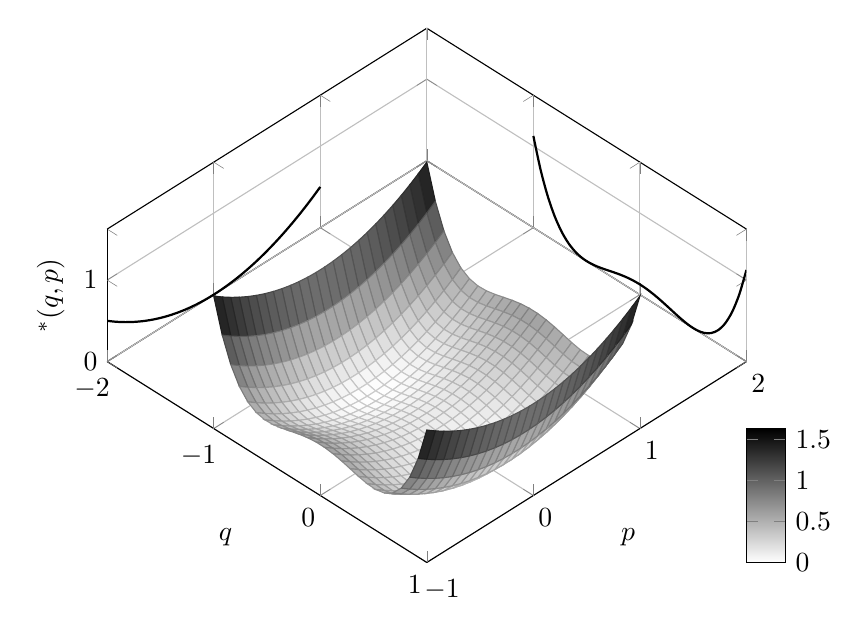
\begin{tikzpicture}[
  declare function = {lambda=2;},
  declare function = {mu=1;},
  declare function = {kin=(x^2)/2;},
  declare function = {pot(\l,\m)=\l*x^4 - \m*x^2 + (\m^2)/(4*\l);},
  declare function = {H(\l,\m)=\l*x^4 - \m*x^2  + (\m^2)/(4*\l)+ (y^2)/2;}]
  \begin{axis}[
    colormap  = {whiteblack}{color(0cm)  = (white);color(1cm) = (black)},
    width          = 0.8\linewidth,
    view           = {45}{65},
    enlargelimits  = false,
    grid           = major,
    domain         = -1:1,
    y domain       = -1:1,
    samples        = 26,
    xlabel         = $q$,
    ylabel         = $p$,
    zlabel         = {$\Ha^*(q,p)$},
    colorbar,
    colorbar style = {
      at     = {(1,0)},
      anchor = south west,
      height = 0.25*\pgfkeysvalueof{/pgfplots/parent axis height},
     % title  = {$P(x_1,x_2)$}
    }
  ]
    \addplot3 [surf] {H(lambda,mu)};
    \addplot3 [domain=-1:1,samples=31, samples y=0, thick, smooth]
     (x,2,{pot(lambda,mu)});
    \addplot3 [domain=-1:1,samples=31, samples y=0, thick, smooth]
      (-2,x,{kin});

    %\draw [black!50] (axis cs:-1,0,0) -- (axis cs:4,0,0);
    %\draw [black!50] (axis cs:0,-1,0) -- (axis cs:0,4,0);

    %\node at (axis cs:-1,1,0.18) [pin=165:$P(x_1)$] {};
    %\node at (axis cs:1.5,4,0.32) [pin=-15:$P(x_2)$] {};
  \end{axis}
\end{tikzpicture}
    \caption[Desired shaped energy function]{Desired shaped energy function $\Ha^*(q,p) = \lambda q^4-\mu q^2 + \frac{1}{2}p^2 + \frac{\mu^2}{4\lambda}$}
    \label{fig:shaped_en}
\end{figure}
%
Thus, 
%
\begin{align}
    \Ha_a & = \Ha^* - \Ha \\
          & = \lambda q^4-(\mu+\frac{1}{2}\kappa)q^2 + \frac{1}{2}p^2 + \frac{\mu^2}{4\lambda}
\end{align}
%
and, therefore
\[\bm\nabla\Ha_a = (4\lambda q^3-(2\mu + k)q,p).\]
It is easy to proof that the matching conditions (\ref{eq:match_lin}) of the EB--PBC are satisfied for $\Ha_a$. The energy shaping control law becomes
%
\begin{align}\label{eq:ex_ctrl}
    \beta(q) &= -\begin{bmatrix}0&1\end{bmatrix}\begin{bmatrix}0&-1\\1&-b\end{bmatrix}\begin{bmatrix}4\lambda q^3-(2\mu + k)q\\p\end{bmatrix}\nonumber\\
             &= -4\lambda q^3+(2\mu + k)q.
\end{align}
%
A numerical simulation of the proposed control scheme has been performed with $k = 1$, $b = 0.5$. The parameters $\lambda$ and $\mu$ have been set to $2$ and $1$ respectively, placing the minima of $\Ha^*$ in $[\pm0.5,0]^\top$. No damping injection actions has been added as the asymptotic stability is already guaranteed by the natural dissipation of the autonomous linear system. Starting in the initial position $\xb_0 \triangleq (-0.9,0)$ the system has been simulated for both the  autonomous and the multistable EB--PBC controlled system for $40s$. The resulting phase--space portraits are reported in Fig. \ref{fig:ctrl_ps}.
%
\begin{figure}[h]
    \centering
    %\definecolor{ocean}{rgb}{0.00000,0.44700,0.74100}

\begin{tikzpicture}
\begin{axis}[
width=5cm,
height=5cm,
at={(1in,0.331in)},
view={0}{90},
%colorbar,
%point meta max=1,
%point meta min=0,
colorbar horizontal,
%colorbar style={
%	width=8cm,
	%xtick={0,0.5,...,30},
%	ylabel style={},
%	xticklabel pos=lower
%},
colormap = {whiteblack}{color(0cm)  = (white);color(1cm) = (black)},
colorbar style = {at = {(0,-0.25)}},
xmin=-1,
xmax=1,
xlabel style={font=\color{white!15!black},at = {(0.75in,-0.1in)}},
xlabel={$q(t)~[m]$},
ymin=-1,
ymax=1,
ylabel style={font=\color{white!15!black},at = {(-0.1in,0.75in)}},
ylabel={$p(t)~[ms^{-1}]$},
title = {uncontrolled},
axis background/.style={fill=white},
]
\addplot3[contour filled={number = 25,labels={false}},mesh/rows=50,mesh/cols=50,mesh/check=false,forget plot
] table {H.dat};
%
\addplot [color=ocean, line width=1.5pt]
table[row sep=crcr]{%
	-0.9	0\\
	-0.899985991795746	0.00501674269174762\\
	-0.899944019691303	0.0100193471557007\\
	-0.899874162931692	0.0150076971406221\\
	-0.89977650140532	0.0199816771641279\\
	-0.898873958295022	0.0446320420072224\\
	-0.897288646861763	0.0689062780415569\\
	-0.8950312582937	0.0927908195727069\\
	-0.892112845290034	0.116272595485913\\
	-0.868002952216995	0.227228035383425\\
	-0.829223766085857	0.326435243373571\\
	-0.777500187200184	0.412807338237014\\
	-0.714659008971771	0.485603292982159\\
	-0.600340602727355	0.570331414933827\\
	-0.471488130080395	0.621495133714803\\
	-0.335347897263502	0.640176352681101\\
	-0.198445114013884	0.628945422916099\\
	-0.0746437735806325	0.594456994280607\\
	0.0401381420897199	0.540383416283467\\
	0.142232199262124	0.470719359197013\\
	0.229035654600393	0.389586456149254\\
	0.290490142676407	0.313265041426897\\
	0.338339729122556	0.23421079930552\\
	0.372303052526759	0.154991891744638\\
	0.392571550535566	0.0778835525828194\\
	0.399731808807902	-0.00306277450207788\\
	0.391870981971099	-0.0763851640723532\\
	0.370660517667212	-0.14009523114136\\
	0.338087981923116	-0.192856605316552\\
	0.298136191440485	-0.232477962681855\\
	0.25184670416552	-0.260834031598041\\
	0.201350587767438	-0.277964416164619\\
	0.148664452554781	-0.284317405805023\\
	0.0907667653016975	-0.27983068280962\\
	0.0349146831770288	-0.264713991318473\\
	-0.0168257578844223	-0.240602883573134\\
	-0.0628664499768871	-0.20930778888674\\
	-0.0980374609679892	-0.17699717235111\\
	-0.127063690395628	-0.141926700215142\\
	-0.149546840710965	-0.105459101422993\\
	-0.165363769927057	-0.0688391130058303\\
	-0.17517242929207	-0.0298002370528735\\
	-0.177436179549933	0.00664995096132089\\
	-0.172778407588365	0.0393477927721653\\
	-0.162032775025325	0.0674497666527798\\
	-0.147454933577949	0.0889207675276733\\
	-0.129347064906398	0.10558047092737\\
	-0.108623814628922	0.117297644237556\\
	-0.086179982857339	0.124136300367046\\
	-0.0599942658276899	0.126273096752299\\
	-0.03394383333752	0.123024483749271\\
	-0.00911017489546286	0.115053707894857\\
	0.0136390018342169	0.103150490035125\\
	0.0323115311721372	0.0893174145892377\\
	0.0481096403624088	0.0735852869681779\\
	0.0607228554124504	0.0566997231192924\\
	0.0700087283561835	0.0393538111534125\\
	0.0761616883827873	0.0213703319404493\\
	0.0787495703594155	0.00429179247670834\\
	0.0780099609822195	-0.0112862674191978\\
	0.0742949609073913	-0.0249184536659205\\
	0.0676235361779361	-0.0368399446136417\\
	0.0587030242407405	-0.0459531423309749\\
	0.0481558122411435	-0.0521341873494105\\
	0.0365928902454288	-0.0554253293582465\\
	0.0240750228983752	-0.0559548535184\\
	0.0117514398745198	-0.0537959330321324\\
	0.00019941613886286	-0.0493329003279672\\
	-0.0101378207178845	-0.0430176266200058\\
	-0.019073150754024	-0.0351836299097121\\
	-0.0261146445062195	-0.0264793026690255\\
	-0.0311080878005064	-0.0174345850654783\\
	-0.0340432057031742	-0.00851368245135384\\
	-0.0350111008169466	0.000208271867982888\\
	-0.034025886560588	0.00794187081482636\\
	-0.0313546321013023	0.014373201383412\\
	-0.0273270827992865	0.0193247845816726\\
	-0.021776682313328	0.0229649845032737\\
	-0.0155344254822122	0.0247149856554559\\
	-0.00909170615632734	0.0246816915211178\\
	-0.00286371969873624	0.0230947709063524\\
	0.00280725028199055	0.0202496734322155\\
	0.00760795718689828	0.016477401614915\\
	0.0113249300742123	0.0121348606754593\\
	0.0138716616756584	0.00755763965809117\\
	0.0153115070918749	0.00268446415992479\\
	0.0154380718037925	-0.00174353700984352\\
	0.0144046855261442	-0.0054393994641403\\
	0.0124469315254243	-0.00824628912471304\\
	0.00973633834811147	-0.0101436953203082\\
	0.00663307131848225	-0.0109904365212177\\
	0.00344345203354436	-0.010849788231025\\
	0.000418598885933671	-0.00987679726686231\\
	-0.00236889674029977	-0.00817147420768934\\
	-0.00455610701932897	-0.00600636910422985\\
	-0.0060212570956228	-0.00363960519553869\\
	-0.00675662344583174	-0.00129708301418448\\
	-0.00679915540873005	0.000997090639439771\\
	-0.00615806076904666	0.0028415988465903\\
	-0.00499448977320246	0.00409954744618751\\
	-0.00350966028254127	0.0047525483255705\\
	-0.00178742736195878	0.00483753431425414\\
	-0.000142544164199142	0.00436296059647222\\
	0.001233863384226	0.00346409628606365\\
	0.00224352413019931	0.0023187867470898\\
	0.00286423019005585	0.001064908755426\\
	0.00304301781878184	-0.000107287213496858\\
	0.00281783500493549	-0.0010575880234264\\
	0.0022937627777237	-0.00172125518888289\\
	0.00153324548129663	-0.00210115118921709\\
	0.000699028537681449	-0.00212944532957787\\
	-7.39090484163769e-05	-0.00185022451593175\\
	-0.000696860580362937	-0.0013673867011887\\
	-0.00115698870029392	-0.000733929244931739\\
	-0.00134549775988726	-0.000103223462323883\\
	-0.00126431291907824	0.000412349861050412\\
	-0.000993032124110712	0.000759026310963054\\
	-0.000596744297566764	0.000936587972301828\\
	-0.0001714552068425	0.000909680277066964\\
	0.000192405808728558	0.000708505171052146\\
	0.000443835290730197	0.000417655115078066\\
	0.000582041712668234	8.20914139281743e-05\\
	0.000563673850896241	-0.000200244790181628\\
	0.000407680747611572	-0.000363593139831435\\
	0.000193602312173417	-0.000405181279185971\\
	-2.30281468151146e-05	-0.000352938747129361\\
	-0.000186564607289939	-0.000224639431191565\\
	-0.000253723590669539	-6.14216529346211e-05\\
	-0.000236476036563678	7.85096220374468e-05\\
	-0.000162705457701936	0.000174617140937539\\
	-5.64067851445571e-05	0.000196804176492543\\
	4.62570015027289e-05	0.000136732345109551\\
	0.000106953605066236	4.5051528543188e-05\\
	0.00012515523979931	-5.30186446630676e-05\\
	8.69067523052607e-05	-0.000109998447934223\\
	-2.80092519366811e-06	-9.06136603478964e-05\\
	-7.20860461539662e-05	-2.64132971781262e-05\\
	-7.64796094496801e-05	2.09540211186838e-05\\
	-5.84460433855426e-05	5.1911771294405e-05\\
	-2.42154646050572e-05	5.68361010025379e-05\\
	8.96341400149207e-06	4.27250166876023e-05\\
}
[postaction={decorate, decoration={markings,
		mark=between positions 0.4 and 1 step 1 with {\arrow[black,line width=1.5pt]{latex};}
}}]
;
\addplot [color=black, line width=1.0pt, draw=none, mark=*, mark options={solid, fill=red}]
table[row sep=crcr]{%
	0	0\\
};
\end{axis}
%
%
%%%%%%%%%%%%%%%%%%%%%%%%%%%%%%%%%%%%%%%%%%%%%%%%%%%%%%%%%%%%%%%%%%%%%%%%%%%%%%%%%%%%
%%%%%%%%%%%%%%%%%%%%%%%%%%%%%%%%%%%%%%%%%%%%%%%%%%%%%%%%%%%%%%%%%%%%%%%%%%%%%%%%%%%%
%%%%%%%%%%%%%%%%%%%%%%%%%%%%%%%%%%%%%%%%%%%%%%%%%%%%%%%%%%%%%%%%%%%%%%%%%%%%%%%%%%%%
%%%%%%%%%%%%%%%%%%%%%%%%%%%%%%%%%%%%%%%%%%%%%%%%%%%%%%%%%%%%%%%%%%%%%%%%%%%%%%%%%%%%
%%%%%%%%%%%%%%%%%%%%%%%%%%%%%%%%%%%%%%%%%%%%%%%%%%%%%%%%%%%%%%%%%%%%%%%%%%%%%%%%%%%%
%%%%%%%%%%%%%%%%%%%%%%%%%%%%%%%%%%%%%%%%%%%%%%%%%%%%%%%%%%%%%%%%%%%%%%%%%%%%%%%%%%%%
%%%%%%%%%%%%%%%%%%%%%%%%%%%%%%%%%%%%%%%%%%%%%%%%%%%%%%%%%%%%%%%%%%%%%%%%%%%%%%%%%%%%
%%%%%%%%%%%%%%%%%%%%%%%%%%%%%%%%%%%%%%%%%%%%%%%%%%%%%%%%%%%%%%%%%%%%%%%%%%%%%%%%%%%%
%%%%%%%%%%%%%%%%%%%%%%%%%%%%%%%%%%%%%%%%%%%%%%%%%%%%%%%%%%%%%%%%%%%%%%%%%%%%%%%%%%%%
%%%%%%%%%%%%%%%%%%%%%%%%%%%%%%%%%%%%%%%%%%%%%%%%%%%%%%%%%%%%%%%%%%%%%%%%%%%%%%%%%%%%
%
%
\begin{axis}[
width=5cm,
height=5cm,
at={(2.7in,0.331in)},
view={0}{90},
%point meta max=1,
%point meta min=0,
colorbar horizontal,
colorbar style = {at = {(0,-0.25)}},
colormap = {whiteblack}{color(0cm)  = (white);color(1cm) = (black)},
xmin=-1,
xmax=1,
xlabel style={font=\color{white!15!black},at = {(.75in,-0.1in)}},
xlabel={$q(t)~[m]$},
ymin=-1,
ymax=1,
ylabel style={font=\color{white!15!black},at = {(-0.1in,0.75in)}},
ylabel={$p(t)~[ms^{-1}]$},
title = {controlled},
axis background/.style={fill=white},
]
\addplot3[contour filled={number = 25,labels={false}},mesh/rows=50,mesh/cols=50,mesh/check=false,forget plot
] table {Hs.dat};
%
\addplot [color=ocean, line width=1.5pt]
table[row sep=crcr]{%
	-0.9	0\\
	-0.899996870908082	0.00502218565295018\\
	-0.899987486315726	0.0100411075881561\\
	-0.899971850372859	0.0150566320023799\\
	-0.899949967395858	0.0200686252832798\\
	-0.899747009487171	0.0450709682895715\\
	-0.899388618721859	0.0699651105069001\\
	-0.89887552042962	0.0947346192697363\\
	-0.898208541398208	0.119363260804648\\
	-0.892600993178684	0.239855894760487\\
	-0.88332728745733	0.354537716060326\\
	-0.870592934007952	0.461743628934238\\
	-0.854651946572982	0.560123643331168\\
	-0.825891178273728	0.68711204984624\\
	-0.791834879838772	0.790728220714818\\
	-0.75356399451932	0.87046177063195\\
	-0.712150640733304	0.927273760461966\\
	-0.66000922437946	0.968001515286153\\
	-0.606351153134016	0.983388496835424\\
	-0.552432399595694	0.978299357428808\\
	-0.499237594212773	0.957805896693751\\
	-0.436098851806087	0.918592641428244\\
	-0.375928948650855	0.870055120877677\\
	-0.319171887540915	0.817588446523111\\
	-0.26597133453238	0.765195191249004\\
	-0.196570877379877	0.696260098511377\\
	-0.133274544560941	0.636807908746945\\
	-0.0751015687653325	0.588831113446346\\
	-0.0209415964564726	0.552814026443317\\
	0.0380018803480918	0.525261548417011\\
	0.09469268769861	0.511231627016708\\
	0.150490028552446	0.50859735000948\\
	0.206491987962548	0.514646517739119\\
	0.263463923517447	0.526124860361028\\
	0.321830340221447	0.538917422041697\\
	0.381469829233457	0.547811078624538\\
	0.441577812926544	0.546564799353567\\
	0.508403847681104	0.524450169126519\\
	0.570473851807155	0.470897518910003\\
	0.623435900817305	0.38076344947073\\
	0.663102610575053	0.25559082405171\\
	0.678302233601095	0.1716016140185\\
	0.687358679603882	0.0830343580824768\\
	0.690057404154059	-0.0061563914658132\\
	0.686524352204035	-0.0920210132729015\\
	0.677159602479465	-0.17078525047383\\
	0.662571377606639	-0.239273019570815\\
	0.643550911614393	-0.295308941997076\\
	0.621019713450437	-0.337882018563323\\
	0.596693663207578	-0.366351138046259\\
	0.570833228097558	-0.382732072077481\\
	0.544233342766672	-0.388145409799201\\
	0.51759169236887	-0.384125181745222\\
	0.486239353795321	-0.369147564138261\\
	0.456501988415763	-0.345590468953559\\
	0.428993677675456	-0.315905947976102\\
	0.404133879978305	-0.282249154373989\\
	0.374973517724411	-0.233046789052566\\
	0.351466108524863	-0.182442447262903\\
	0.333664394576861	-0.132360703391403\\
	0.321453908231802	-0.0839374118527956\\
	0.312973603910283	-0.011921561839968\\
	0.316880430268802	0.0542583374859615\\
	0.332048531823487	0.114156778557127\\
	0.35724898945573	0.166391177582508\\
	0.390551439317867	0.20821286331742\\
	0.430037954813706	0.23573955388851\\
	0.472645672033786	0.243581013484698\\
	0.514529160660574	0.22674602198758\\
	0.536961635024244	0.203869304233178\\
	0.556519841618899	0.171777393936242\\
	0.57227356607027	0.131715097983101\\
	0.583548661291591	0.0856499230661991\\
	0.588660261399382	0.0499970798263594\\
	0.591067043796994	0.0139325769543233\\
	0.590778287019473	-0.0212719592529122\\
	0.587909612896141	-0.054437952782987\\
	0.582662116929988	-0.0845091654449368\\
	0.575301356749247	-0.110599533937668\\
	0.566148074574292	-0.132076851694419\\
	0.555561238935455	-0.148604004678177\\
	0.542727363495747	-0.160963577098416\\
	0.529122643361111	-0.167389582112847\\
	0.515223845930749	-0.168261600752074\\
	0.501460255529128	-0.164182597505957\\
	0.485459184718837	-0.153607782543439\\
	0.470781727499624	-0.138029112333493\\
	0.457876588001754	-0.118677429918171\\
	0.447055487685268	-0.0967359360501288\\
	0.437750202462486	-0.0707004439545602\\
	0.431386741252715	-0.0438544372397111\\
	0.42800939659567	-0.0171672159885568\\
	0.427550667839335	0.00856308856880236\\
	0.429856483241429	0.0326759363757232\\
	0.434717427706793	0.0545303878640252\\
	0.441850842628459	0.0735290409265509\\
	0.450909672023688	0.0891317624569311\\
	0.462836674329704	0.101957161215865\\
	0.476009320526056	0.109219750949453\\
	0.489696458337837	0.110435129918282\\
	0.503151333204252	0.105416956461234\\
	0.515019779810078	0.095024686876189\\
	0.525358354731631	0.0797100705833284\\
	0.533614900870741	0.0603869473648223\\
	0.539419905552243	0.0382594909132976\\
	0.542562025129876	0.014787701208899\\
	0.54294846455292	-0.00831716740492562\\
	0.54068641355371	-0.0294935781181016\\
	0.536098923460489	-0.0474963526010204\\
	0.530956259767132	-0.0591732071470334\\
	0.524841684656134	-0.0677801518344928\\
	0.518056730633023	-0.0731676285577933\\
	0.510905294408393	-0.075388849364275\\
	0.502993469071269	-0.0744283299121389\\
	0.495357358384163	-0.0702620285699195\\
	0.488315299129287	-0.0633548100691062\\
	0.482119232463464	-0.0542635129531932\\
	0.476202571553501	-0.041645145451146\\
	0.471927928938389	-0.0276802614081685\\
	0.469423255586312	-0.0131963227104877\\
	0.46869388106308	0.0010535865854046\\
	0.469654044686674	0.0144165262888192\\
	0.47216787179427	0.0262855311149465\\
	0.476025187735923	0.0361366148834856\\
	0.480951328271342	0.0435849276075637\\
	0.486688525777316	0.0483895901410702\\
	0.492835917741696	0.050256421243311\\
	0.499021244133837	0.0491421430332563\\
	0.50489283191071	0.0451965046164959\\
	0.511495556389668	0.0364617764383878\\
	0.516433201933496	0.0246750217794874\\
	0.5192715070456	0.0112163249849652\\
	0.519919534284879	-0.00245654830435253\\
	0.518865257072046	-0.0130791849559421\\
	0.516492805358045	-0.0219935791230009\\
	0.513057621127676	-0.0286080414697376\\
	0.508896858782351	-0.0326384758704046\\
	0.504921559764719	-0.0340140370830793\\
	0.500904672954963	-0.0334067949557782\\
	0.497074634328902	-0.0309922701874025\\
	0.493623081079446	-0.0270581187025049\\
	0.489695005894198	-0.0196566671679421\\
	0.487127221100895	-0.0108900508947703\\
	0.486105059728068	-0.0017316322583785\\
	0.486574088439371	0.00685446669200195\\
	0.488038305638497	0.0132420015624049\\
	0.490322971009597	0.0181942070340653\\
	0.49320491981277	0.0213962116930026\\
	0.496419577640723	0.0227278197419268\\
	0.499606839935091	0.0222508852572002\\
	0.502605382335153	0.020128098231039\\
	0.505191909728477	0.0165927562257983\\
	0.507203573375784	0.0119977453361008\\
	0.508570407414329	0.00656210642742873\\
	0.509125903842199	0.000953293386108705\\
	0.50886593306216	-0.00432891904143036\\
	0.507881846287006	-0.00887046683221743\\
	0.50632088227945	-0.0123602182259025\\
	0.504346759779108	-0.014561017527977\\
	0.502151670509713	-0.0153658246666499\\
	0.499933819445742	-0.0148433019832304\\
	0.497810963376916	-0.0131035149576992\\
	0.49603077804738	-0.0103689351788658\\
	0.49472970754404	-0.00694185473360482\\
	0.493974255339596	-0.00317964820510094\\
	0.493777155710845	0.000674916255547264\\
	0.49415233496808	0.00418167410046676\\
	0.495033347632413	0.00704185983405202\\
	0.496297197301268	0.00906244795975967\\
	0.49779707628873	0.0101433518689256\\
	0.49938420139213	0.0102301598989902\\
	0.500906207933653	0.00936357826989489\\
	0.502232075492357	0.0076988655989565\\
	0.503459988008728	0.00487289975083279\\
	0.504098787382893	0.0016274430961605\\
	0.504084878850324	-0.00155179804524677\\
	0.503501223258307	-0.00422748500218759\\
	0.502576674792561	-0.00600016698786394\\
	0.501416793948805	-0.00688393874992451\\
	0.500179347125908	-0.0068167790803002\\
	0.499025423479739	-0.00592106070586954\\
	0.498098300367774	-0.00444301600834487\\
	0.497471127067439	-0.00257262825390797\\
	0.497203150072829	-0.000553688507107395\\
	0.497286146602341	0.00135936404988428\\
	0.497748482151337	0.0031846201013095\\
	0.498515012404264	0.00434588955665634\\
	0.49945284482695	0.00468356992260722\\
	0.500387351232607	0.00425061686996816\\
	0.501096376952997	0.00334924411116571\\
	0.501604039713047	0.00210049585964706\\
	0.501853900209779	0.000685192300734486\\
	0.501843764920484	-0.00069611883662297\\
	0.501520909428211	-0.00216199060026829\\
	0.500924774621535	-0.00303881336585789\\
	0.500179139865576	-0.00315788068393117\\
	0.499473955185514	-0.00260820481990068\\
	0.499034161875787	-0.00180629798636776\\
	0.498771843947808	-0.000821708406309548\\
	0.498717288854108	0.00019478437333335\\
	0.498852267133584	0.00108973178760345\\
	0.499201686787063	0.00187571346471635\\
	0.499680012144524	0.00219142062624092\\
	0.500187226526845	0.00197396252564304\\
	0.500600584775413	0.00135452239798497\\
	0.500823128603035	0.000623077831361884\\
	0.50088126747437	-0.000143613630490948\\
	0.500769733967566	-0.000809192560811333\\
	0.50053334017428	-0.00126543698401065\\
	0.500199475863577	-0.00147854519940249\\
	0.499858278290114	-0.00135467012813077\\
	0.499582046290141	-0.000921038392843261\\
	0.499427331959661	-0.000331021833538781\\
	0.499408752613925	0.000274225090242636\\
	0.499528471648617	0.000751896997551173\\
	0.499760969015216	0.000992120046342246\\
	0.500026199046028	0.000966904068969492\\
	0.50024428477368	0.000735625678594537\\
	0.500384966463704	0.000365742726126805\\
	0.50041706074676	-6.14606882469497e-05\\
	0.500349267319465	-0.00042887605319836\\
	0.500211891046477	-0.000663331994049548\\
	0.500039148910993	-0.000716004902349041\\
	0.499870454534924	-0.000571870286033578\\
	0.499752046398847	-0.000301650448253914\\
	0.499706671952549	-1.25850887606945e-06\\
	0.499735322241737	0.000267408945444464\\
	0.499832580606591	0.000441805752959287\\
	0.499960844816268	0.00048800100258279\\
	0.500097700605659	0.00040750633498734\\
	0.500190626229716	0.000211616022071412\\
	0.500210076325697	-5.45402232100384e-05\\
	0.50015779031305	-0.000275729639607801\\
	0.500063297000641	-0.0003802938243217\\
	0.499958512676221	-0.000354553459092898\\
	0.499872193957112	-0.000193009529218423\\
	0.499838674451653	1.94299393468682e-05\\
	0.499862716694351	0.000192828627862818\\
	0.499927458094128	0.000287974503273678\\
	0.500018504392869	0.00027014968054408\\
	0.50009416410398	0.000160514931820332\\
	0.500130804216567	7.50332254610063e-06\\
	0.500118312081449	-0.000133734199216639\\
	0.50005345438149	-0.00021907855656711\\
	0.499973123468112	-0.000210631882879923\\
	0.499901430102954	-0.000123417785712298\\
	0.499876682611882	1.53804353494455e-05\\
	0.499920923193596	0.000178096715164343\\
	0.500007295829889	0.000240355921040274\\
	0.500087011639498	0.000169691058559411\\
	0.50012524738499	3.22663512008806e-05\\
	0.500099528285922	-0.000145251295293692\\
	0.500025157032281	-0.000242175244369207\\
	0.499941989242554	-0.000215534860408795\\
	0.499888225963651	-9.93392139943571e-05\\
	0.499888436350962	9.32685096879741e-05\\
	0.499945076519787	0.000230645044714538\\
	0.49996873075281	0.000236250827185643\\
	0.499992452973781	0.000232230793866627\\
	0.500015287760057	0.000219190889408761\\
	0.500036393945116	0.000198108040130646\\
}
[postaction={decorate, decoration={markings,
		mark=between positions 0.3 and 1 step 1 with {\arrow[black,line width=1.5pt]{latex};}
}}]
;
\addplot [color=black, line width=1.0pt, draw=none, mark=*, mark options={solid, fill=red}]
table[row sep=crcr]{%
	0	0\\
	-0.5 0\\
	0.5 0\\
};
\end{axis}
\end{tikzpicture}
    %
    %\vspace{-7mm}
    \caption[Phase--space portraits of the autonomous and the multistable EB--PBC controlled system]{Comparison of the phase--space portraits of the autonomous and the multistable EB--PBC controlled system with $k = 1$, $b = 0.5$, $\lambda = 2$, $\mu = 1$. The phase--space portraits are represents over contour plots of the corresponding energy functions, i.e., $\Ha = \frac{1}{2}(kq + p)$ and  $\Ha^* =  2q^4 - q^2 + \frac{1}{2}p + \frac{1}{8}$. The red dots indicates the critical points of $\Ha$ and $\Ha^*$.}
    \label{fig:ctrl_ps}
\end{figure}
%
\iffalse
Note that the damping injection control action $v = -ky$ does not change the location of the fixed points of the system. 
%{\color{red}
\begin{prop}\label{prop:db_lin}
Let $u = v$ ($\beta(x) = \mathbb{0}_m$), it holds:
%
\[\mymathbb{0}_n = Ax - k BB^\top Px = \left(A-kBB^\top P\right)x\]
if and only if $x = \mymathbb{0}_n$.
%
\end{prop}
%
%
\begin{proof}
Necessary and sufficient condition to have 
\[\mymathbb{0}_n = \left(A-kBB^\top P\right)x~\Leftrightarrow~x = \mathbb{0}_n\]
is the matrix $A-kBB^\top P$ to be full--rank. 
Let $S = kBB^\top P$ which is positive semi--definite for $k>0$ since $P>0$. In particular, $\rank(S) = m$ because $P$ is full--rank and $\rank(B) = m$. Since $A$ is full--rank, it holds:
\[\rank(A-S) + \dim[\Null(A-S)] = \rank(A)\]
Furthermore, 
\[\Null(A-S) = \Null(I_n - A^{-1}S)\]
Thus, $A-S$ is full--rank if and only if 
\[\det(I_n - A^{-1}S)\neq 0\]
Indeed, $A^{-1}S$ is negative semi--definite since $A<0$ and $S\geq 0$. Let $p(s)$ be characteristic polynomial of $A^{-1}S$, i,e,
\[p(s) = \det(A^{-1}S - sI_n) = \prod_{i = 1}^n(\alpha_i-s) = (-1)^n\prod_{i = 1}^n(s-\alpha_i)\]
where $\alpha_i$ ($i = 1,\dots,n$) are the eigenvalues of $A^{-1}S$.
Hence, by setting $s = 1$, yields
\[\det(I-A^{-1}S) = (-1)^n(-1)^n\prod_{i = 1}^n(1-\alpha_i) = \prod_{i = 1}^n(1-\alpha_i)\]
Since $\alpha_i\leq 0~\forall i = 1,\dots,n$, the product is strictly positive and this proves $\det(I_n - A^{-1}S)\neq 0$. Therefore, $\dim[\Null(A-S)] = 0$ and, eventually,
\[\rank(A-kBB^\top P) = \rank(A) = n\]
which proves the proposition.\\
$\blacksquare$
\end{proof}
%
A similar proposition can be proved in the case of the energy--shaping controlled linear system, i.e. $\beta(x) = B^+(J-R)\partial\Ha_a$, using the port--Hamiltonian form of the model.
\begin{prop}
Let the energy--shaping controlled system be:
\begin{align*}
    &\dot{x}=(J-R)\partial\Ha^* + Bv\\
    &y = B^\top\partial\Ha^* 
\end{align*}
The control law $v = -ky$ does not modify the fixed points of the system i.e.
\[\mathbb{0}_n=(J-R)\partial\Ha^*-kBB^\top\partial\Ha^*=\left[(J-R)-kBB^\top\right]\partial\Ha^*\]
if and only if $\partial\Ha^*=0$.
\end{prop}
\begin{proof}
As in Proposition \ref{prop:db_lin}, the necessary and sufficient condition so that the previous statement holds is equivalent to asking if the matrix $(J-R)-kBB^\top$ is full--rank.
Recalling that $J-R=AP^{-1}$, it holds:
\begin{align*}
    \rank(J-R-kBB^\top) &= \rank[(J-R-kBB^\top)P]\\
    &=\rank(A-kBB^\top P)\\
    &=\rank(A)=n
\end{align*}
thanks to Proposition \ref{prop:db_lin}.\\
$\blacksquare$
\end{proof}
\fi
%
\subsection{Choice of the Dissipation Rate: Shaping the basins of attraction}
%
In this section it is shown how, by tuning the dissipation rate $\mathbf{K_d}$, it is possible to shape the basins of attraction of the designed stable fixed points of the closed--loop system.
%
\begin{defn}
The \textit{basin of attraction} $\B$ of a fixed point $\xb^*$ of a system (\ref{eq:nlaffine}) is the set of all initial conditions $\xb_0$ leading to long--time behavior that approaches that fixed point, i.e.
%
\begin{equation*}
    \B \triangleq \left\{\xb_0\in\X|\lim \limits_{t\rightarrow\infty}\Phi(t,\xb_0,\ub)=\xb^*\right\}.
\end{equation*}
%
\end{defn}
%
The designed feedback control law (\ref{eq:ex_ctrl}) allows to fix multiple stable points for the closed--loop system. The damping injection component of the overall control action can be used to ``shape'' their basins of attraction. This property allows to have interesting control actions which will be qualitatively shown.
%
Consider the system of Example \ref{ex:msd_MES} controlled by the energy shaping control law (\ref{eq:ex_ctrl}). The closed--loop system in the form (\ref{eq:nlaffine}) can be expressed as
%
\begin{equation*}
	\left\{
    \begin{matrix*}[l]
    \dot{\xb} = \begin{bmatrix}p\\-4\lambda q^3+2\mu q-bp\end{bmatrix} + \Bb v\\
    y = \Bb^\top \Pb\xb
    \end{matrix*}
    \right. .
\end{equation*}
%
If $v= 0$ the system has two asymptotically stable fixed points in $[\pm\sqrt{\mu/2\lambda},0]^\top$.Let $\mathbf{K}_d \triangleq k_d$. The output feedback controller $v = -k_d y = -k_dp$ does not change the location of the fixed points. In facts, it only changes the overall dissipation of the system from $bp$ to $(b+k_d)p$.
%
Besides, the respective basins of attraction strongly depend on the choice of the controller, i.e., on the value of $k_d$. In Fig. \ref{fig:basin} the basins of attraction of the two fixed points are shown for different values of $k_d$ in the region $[-1,1]\times [-1,1]$ of the state space with $b = 0$, $\lambda = 2$, $\mu = 1$. It is evident that the higher the dissipation rate is, the lower is the number of transitions between basins of attraction.
%
\begin{figure*}[h]
	\centering
	%\includegraphics[width=\textwidth]{Figures/basin33.eps}
	%\includegraphics[scale=0.5]{basin4}
	\caption{Basins of attraction of the fixed points of the system for different values of $k_d$ in the region $[-1,1]\times [-1,1]$. The basin of attraction of the minima [blue points] are represented in dark gray ($[-0.5,0]^\top$) and light hatched gray ($[0.5,0]^\top$).}
	\label{fig:basin}
\end{figure*}
%
%\fi
\iffalse
{\color{red}
Therefore, given an initial condition $x_0$, and a desired set point $x_i^*$, corresponding to one of the minima of $\Ha^*$, we would be interested in choosing a dissipation rate $\kappa$ such that $x_0$ 
belongs to the basin of attraction $\mathcal{B}_i$ of $x_i^*$ ($\mathcal{B}_i = \mathcal{B}_i(\kappa)$). 
%{\color{red}
%From now on, we will consider the topology on $\R^n$ to be the \textit{standard} one, i.e. the one induced by the euclidian metric. Furthermore, given an open set $\mathcal{S}\subset\R^n$, let us denote its closure with $\bar{\mathcal{S}}$.
%%
%\begin{thm}(Necessity)
%Let $c$ be the initial energy, $c = \Ha^*(x_0)$. Let $\Lambda_c$ be the $c$--level set of $\Ha^*$, $\Lambda_c = \{x|\Ha^*(x)=c\}\subset\R^n$. If there exists a $k\geq 0$ such that $x_0\in\mathcal{B}_i$, then one of the following is necessarily satisfied:
%\begin{itemize}
%    \item[$1.$] $\Lambda_c$ is connected and 
%    \[\exists \Gamma:\partial \Gamma = \Lambda_c ~\land~ x_i^*\in \bar{\Gamma}\]
%    \item[$2.$] $\Lambda_c$ is not connected but it is the union of $p$ connected sets $\Lambda^1_c,\dots,\Lambda^p_c$ and
%    \[\exists {\Gamma}_j:\partial \Gamma_j = \Lambda_c^j ~\land~ x_0,x_i^*\in \Bar{\Gamma}_j\]
%\end{itemize}
%\end{thm}
%\pf
%Due to dissipativity of the controlled system, i.e.
%\[\frac{d\Ha^*}{dt}\leq 0\quad\forall k\geq 0\]
%the any trajectory with initial condition will lie inside the closure of the set $\Gamma$ defined as 
%\[\partial \Gamma \triangleq {L}_c\Ha^*\]
%regardless on the choice of $k$, i.e.,
%\[\Phi(t,x_0,u)\in \bar{\Gamma}\quad\forall t,~\forall k\geq 0\]
%Therefore, if $x_i^*$ does not belong to $\bar{\Gamma}$, it is impossible to reach it, i.e., there is no positive $k$ such that $x_0$ belongs to the basin of attraction of $x_i^*$. If ${L}_c\Ha^*$ is connected also $\bar{\Gamma}$ is connected and $x_0\in\partial \Gamma\subset \bar{\Gamma}$, then the necessary condition for the existence of a $k\geq 0$ such that $x_0\in\mathcal{B}_i$ is simply: $x_i^*\in \bar{\Gamma}$. On the other hand if ${L}_c\Ha_a$ is not connected but it is the union of connected sets, the trajectory will never leave the set $\bar{\Gamma}_j$ defined by 
%\[\partial \Gamma_j \triangleq {L}_c^j\Ha^*\]
%where
%\[{L}_c\Ha^* = \bigcup_{k = 1}^m{L}_c^k\Ha^* \text{ and }x_0\in{L}_c^j\Ha^* \] 
%Thus, the necessary condition is that also $x_i^*$ belongs to $\bar{\Gamma}_j$.\\ 
%$\blacksquare$
%\endpf
%A graphical representation of this necessary condition is given in Fig. \ref{fig:nec}.
%\begin{figure}
%    \centering
%    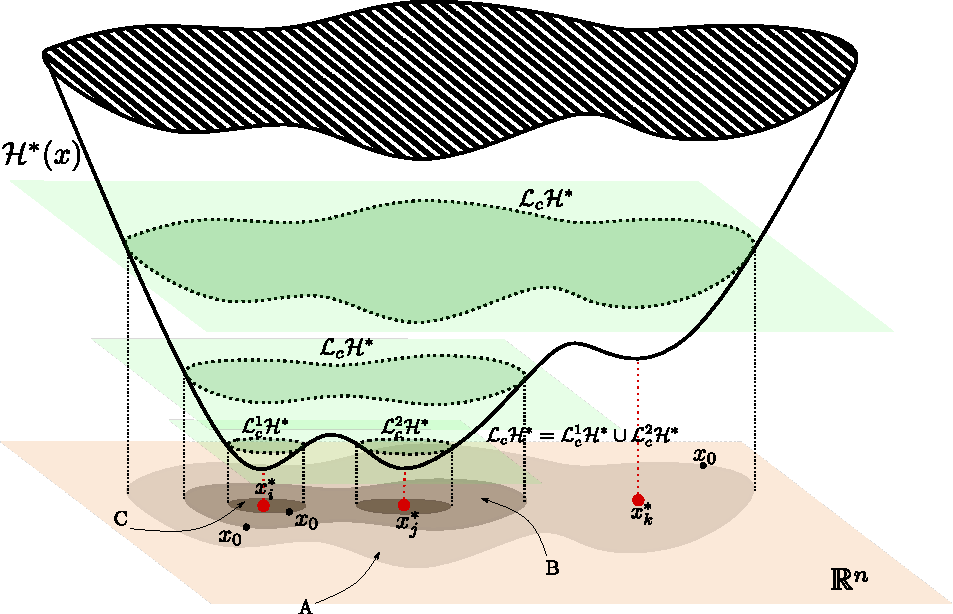
\includegraphics[scale = 0.5]{draw3.pdf}
%    \caption{\footnotesize Graphical representation of the necessary condition given by Theorem 5. Case (A): the condition is satisfied for all the stable fixed points $x_i^*,~x_j^*$ and $x_k^*$. Case (B): the condition is satisfied for $x_i^*,~x_j^*$ but not for $x_k^*$. Case (C): the condition is satisfied only for $x_i^*$.}
%    \label{fig:nec}
%\end{figure}
%}
In order to choose among the possibly infinite values of $\kappa$ such that  $x_0\in\mathcal{B}_i$, one could minimise the damping injection control effort needed to bring $x(t)$ from $x_0$ to $x_i^*$, i.e.,
\[\min_\kappa\int_0^\infty \kappa^2x^\top(s)PBB^\top Px(s)ds\]
This optimisation problem can be simply solved by minimising $\kappa$ such that $x_0\in\mathcal{B}_i(\kappa)$  
\begin{equation*}
\begin{aligned}
& \underset{\kappa}{\text{minimize}}
& & \kappa \\
& \text{subject to}
& &\lim\limits_{t\rightarrow\infty}\Phi(t,x_0,\beta(x)-\kappa B^\top Px)=x^*_i
\end{aligned}
\end{equation*}
This strategy indeed minimises the damping injection control effort but, however, inevitably leads to long transient behaviours depending on the natural dissipation of the system $x^\top PA x$.

Instead, it would be possible to choose on optimal value of $\kappa$ which instead minimises the approaching time to the desired fixed point, i.e., by solving the constrained optimisation problem:
%
\begin{equation*}
\begin{aligned}
& \underset{\kappa}{\text{minimize}}
& & t_a \\
& \text{subject to}
& & \left\{
\begin{matrix*}
\lim\limits_{t\rightarrow\infty}\Phi(t,x_0,\beta(x)-\kappa PBx)=x^*_i\\
\Phi(t_a,x_0,\beta(x)-\kappa PBx)\in\delta_\rho x_i^*
\end{matrix*}
\right.
\end{aligned}
\end{equation*}
%
where $\delta_\rho x^*_i$ is an open neighborhood of $x_i^*$ of radius $\rho$.

Note that the two optimisation problems mentioned above can be easily solved with any numerical algorithm by approximating the constraints as
\begin{align*}
    \lim\limits_{t\rightarrow\infty}&\Phi(t,x_0,\beta(x)-\kappa PBx)=x^*_i\\    
    &\Rightarrow \|\hat{\Phi}(T,x_0,\beta(x)-\kappa PBx)-x^*_i\|_2\leq\varepsilon
\end{align*}
%
where $\hat{\Phi}$ is the numerically integrated trajectory of the system, $T\gg 1$ is the integration time and $\varepsilon \ll 1$ is a chosen threshold.
Similarly,
\begin{align*}
    \Phi(t_a,&x_0,\beta(x)-kPBx)\in\delta_\rho x_i^*\\    
    &\Rightarrow \|\hat{\Phi}(t_a,x_0,\beta(x)-kPBx)-x^*_i\|_2\leq\rho
\end{align*}
}
\fi
%
%
\section{Hybrid Mode Selector}
%
Once the feedback law and the damping injection are designed to produce the desired working modes and to shape their basins of attraction, the proposed strategy aims to switch from a working mode to another.
In particular, considering the system to be in one of the working modes $\xb_i^*$, a control action which moves the system to another desired mode, $\xb_j^*$, is designed.
The strategy reckons on the following actions:
\begin{itemize}
    \item [1.] Switch-off the energy shaping controller (the system turns back linear);
    \item [2.] Give an impulse to the system to bring the state inside the basin of attraction of $\xb_j^*$;
    \item [3.] Switch on again the energy shaping controller.
\end{itemize}
%
\subsection{Impulse generation}
When the nonlinear controller $\ub=\bm\beta(\xb)+\vb$ is switched off, i.e. $\ub=\mymathbb{0}_m$, the system turns back in the LTI form (\ref{eq:lsys}).
Without loss of generality, let $t = 0$ and let the LTI system be controllable. The response of the system to a weighted impulse input 
%
\begin{equation}
\ub(t) = \bm\nu\delta(t)
\end{equation}
%
where $\bm\nu\in\R^m$ distributes the Dirac delta function $\delta(t)$ among the $m$ inputs,
is
%
\begin{align}\label{eq:impresp}
    \xb(t) &= e^{t\Ab}\xb_0 + \int_0^te^{(t-s)\Ab}\Bb \ub(s)ds =\nonumber\\
    &= e^{t\Ab}\xb_0 + \int_0^te^{(t-s)\Ab}\Bb\bm\nu\delta(s)ds \nonumber\\
    &= e^{t\Ab}\xb_0 + e^{t\Ab}\Bb\bm\nu\\
    &= e^{t\Ab}\left(\xb_0 + \Bb\bm\nu\right) .
\end{align}
%
Since the control objective is to move the system from $\xb_i^*$ to $\xb_j^*$ in a time $t^*$, it is tempting to impose the desired behaviour in (\ref{eq:impresp}) by requiring:
%
\begin{equation}\label{eq:cond}
    \xb_j^* \triangleq \xb(t^*) = e^{t^*\Ab}\left(\xb_i^* + \Bb\bm\nu\right).
\end{equation}
%
Therefore, $\bm\nu$ might be obtained as
\begin{align}
    \bm\nu = \left(\Bb^\top\Bb\right)^{-1}\Bb^\top(e^{-t^*\Ab}\xb_j^*-\xb_i^*).
\end{align}
%
However, unless $m = n$, (\ref{eq:cond}) is overdetermined, i.e. $n$ (scalar) equations with only $m$ unknowns (the components of $\bm\nu$). 
To overcome this issue, the design of the impulse controller is achieved by solving the following optimisation problem: 
find $t^*$, $\bm\nu$ such that 
%
\begin{equation}\label{eq:opti}
\begin{aligned}
& [t^*,\bm\nu] = \argmin\limits_{t^*,\bm\nu}\gamma\left\|\bm\nu \right\|^2_2+\rho\left\|\xb_j^* - e^{t^*\Ab}\left(\xb_i^*+\Bb\bm\nu\right)\right\|^2_2\\
& \text{subject to} ~~\bm\varphi\left(t^*,\xb_i^*,\bm\nu\delta(t)\right)\in\B_j
\end{aligned}
\end{equation}
where $\gamma,~\rho\in \R^+$ are two arbitrary weights and  $\B_j$ is the basin of attraction of $\xb_j^*$. 
The term $\gamma\|\bm\nu\|_2^2$ has been introduce for regularization since, in some cases, it might be convenient to simultaneously minimise also the squared norm of the impulse weights.
%

The solution of (\ref{eq:opti}), provides an impulsive input  $\ub = \bm\nu\delta$ which guarantee that the system will arrive in $\B_j$ in a time $t^*$.  
For the sake of a latter numerical implementation, the constraint was defined as
\begin{align}
    \left\|\hat{\bm\varphi}\left(t_{\infty},e^{t^*\Ab}\left(\xb_i^*+\Bb\bm\nu\right),\bm\beta(\xb)-\mathbf{K}_d\Bb^\top \Pb\xb\right)-\xb^*_j\right\|_2\leq\varepsilon
\end{align}
%
where $\hat{\bm\varphi}$ is the numerically integrated trajectory of the system, $t_\infty\gg 1$ is the integration time and $0\leq\varepsilon \ll 1$ is a chosen threshold.
%
\begin{rem}
	Assuming that the switch is performed only at steady--state, the optimisation of $\bm\nu$ and $t^*$ for each pair of fixed points $\xb_i$, $\xb_j$ can be performed off--line.
\end{rem}
%
%%%%%%%%%%%%%%%%%%%%%%%%%%%%%%%%%
\subsection{Overall Hybrid System}
%
If an impulse is applied to the system at time $t$  in order to reach the desired destination $\xb_j^*$, in the instant of time in which the impulse is applied, the state undergoes to a discontinuous jump
%
\begin{equation}\label{eq:jump}
    \xb^+ = \xb(t) + \Bb\bm\nu.
\end{equation}
%
Therefore, the controlled system can be described as an \textit{hybrid automata}, with two logic states $\Sa_1$ and $\Sa_2$. In $\Sa_1$ the system is controlled with the multistable EB--PBC and in $\Sa_2$ the system is completely uncontrolled. Thus, by introducing a timer $\tau$ and an external asynchronous signal $r$ (initialised to $0$), the transition from $\Sa_1$ to $\Sa_2$ will happen when $r$ changes from $0$ to the index of the desired fixed point, i.e., $r\in\{0,1,\dots,p\}$, with a state jump described by (\ref{eq:jump}) and resetting the timer $\tau$ to $0$. Then the system will remain uncontrolled (and thus linear) for a time $t^*$, i.e. $\tau = t^*$ after which the logic state will switch back from $\Sa_2$ to $\Sa_1$  and the timer and the external signal $r$ will be reset. A graphical representation of the designed hybrid automata is given in Fig. \ref{fig:automata}. 
%
\begin{figure}[h]
	\centering
	%\scalebox{0.9}{
\begin{tikzpicture}
	\footnotesize
	%
	% 
	\fill[gray!20, draw = black,thick] (-1.95,0) ellipse (1.5cm and 1cm);
	\fill[gray!20, draw = black,thick] (1.95,0) ellipse (1.5cm and 1cm);
	%	
	\draw (-1.95,0) node[align = center](flow)  {$\begin{bmatrix}
\dot{x}\\\dot{\tau}\end{bmatrix} = \begin{bmatrix}Ax+Bu\\0\end{bmatrix}$\\$u = \beta(x)-\kappa B^\top Px$};
	\draw (1.95,0) node[align = center](flow)  {$\begin{bmatrix}
\dot{x}\\\dot{\tau}\end{bmatrix} = \begin{bmatrix}Ax\\1\end{bmatrix}$};
	%
	\draw [thick,-latex] plot [smooth, tension=1.2] coordinates { (-1,0.76) (0,1) (1,0.76)};
	\draw [thick,-latex] plot [smooth, tension=1.2] coordinates { (1,-0.76) (0,-1) (-1,-0.76)};
	%
	\draw (1.9,1.4) node {$\begin{bmatrix}x^+\\\tau^+\end{bmatrix} = \begin{bmatrix}x+B\nu\\0\end{bmatrix}$};
	\draw (1.6,-1.2) node {$\tau = t^*\land x\in\mathcal{B}_r$};
	%
	%
	%\draw (-1.9,-1.1) node {$\omega^+ = \nu_{w}(x,\omega)$};
	\draw (-1.1,1.1) node {$r \neq 0$};
	\draw (-1.1,-1.2) node {$r = 0$};
	\draw (-3.7,0) node {$\mathcal{S}_1$};
	\draw (3.7,0) node {$\mathcal{S}_2$};
	%
	\end{tikzpicture}}
	\caption{Hybrid automata representing the overall controlled system with the hybrid mode selector.}
	\label{fig:automata}
\end{figure}
%
\clearpage
%%%%%%%%%%%%%%%%%%%%%%%%%%%%%%%%%%%%%%%%%%%%%%%%%%%%%%%%%%%%%%%%%%%%%%%%%%%%%%%%%%%%%%%%%%%%%%%%
\section{Hybrid Port--Hamiltonian Model and Stability}
%
From the hybrid automata representation of Fig. \ref{fig:automata} the extended hybrid port--Hamiltonian model can be obtained. First, the system has two PH flows: one when the system is controlled via multistable EB-PBC
%
\begin{equation}
    \dot{\xb} = \Ab\Pb^{-1}\bm\nabla\Ha_1(\xb) + \Bb\vb
\end{equation}
%
and one when the controller is switched-off
%
\begin{equation}
    \dot{\xb} = \Ab\Pb^{-1}\bm\nabla\Ha_2(\xb)
\end{equation}
%
By introducing a dummy variable $s$, representing the logic state of the system, i.e. $s = i$ in $\Sa_i$, and performing a state extension:
%
\begin{equation}
    \zb \triangleq \left(\xb, \tau,r,s\right)
\end{equation}
%
the flow set can be defined as the union of two subsets $\C_1$ and $\C_2$ corresponding to the logic states of the system, i.e.
%
\begin{equation}
    \C \triangleq \C_1\cup\C_2
\end{equation}
%
where
%
\begin{equation}
    \C_i\triangleq \{\zb: s = i\}.
\end{equation}
%
The port--Hamiltonian set--valued mapping $\F_{\tt PH}$ can be then defined as
%
\begin{equation}
48
\end{equation}
%
\clearpage
%%%%%%%%%%%%%%%%%%%%%%%%%%%%%%%%%%%%%%%%%%%%%%%%%%%%%%%%%%%%%%%%%%%%%%%%%%%%%%%%%%%%%%%%%%%%%%%%
\section{Numerical Simulation}
%
A numerical simulation of the overall controlled system has been performed to validate the proposed control scheme. The whole procedure has been implemented in the \textsc{Matlab}\textsuperscript{\textregistered}%\footnote{The source code is available at \url{https://github.com/massastrello/MultistableControl}.} 
environment. The system introduced in Example \ref{ex:msd_sys} has been controlled with the multistable energy shaping (\ref{eq:ex_ctrl}) and the damping injection $v = -\kappa\dot{\xi}$. The system parameters has been chosen as $k = 5$, $b = 0.5$ and, as in the example in Section \ref{sec:multistable}, the minima of $\Ha^*$ have been positioned in $[\pm 0.5,0]^\top$ by setting $\lambda = 2$ and $\mu = 1$.
{%\color{red}
To implement the asynchronous external control signal $r$, the two fixed points have been denoted with $\xb_1^* = [-0.5,0]^\top$ and $\xb_2^* = [0.5,0]^\top$.}
The dissipation rate $k_d$ has been set to $4.5$. 
The \textit{fmincon} solver of the \textit{global optimization toolbox} of \textsc{Matlab}\textsuperscript{\textregistered} has been employed to solve the optimisation problem (\ref{eq:opti}). The optimisation parameters have been chosen as $t_\infty=10^3$, $\varepsilon=10^{-5}$, considering an absolute tolerance of $10^{-6}$ for the numerical integration (ODE45).
Starting from the initial state $\xb_0 \triangleq [-0.8,0]^\top$, the system, controlled with the nonlinear state feedback and the damping injection, has been integrated until secured convergence to $\xb_1^*$ ($5s$). Then, $r$ has been set to 2 in order to trigger the change of working mode, i.e. to bring the state to $\xb_2^*$. After the jump, the system has been let flowing uncontrolled for a time $t^*$ and then the nonlinear controller has been turned on again. After other $5s$ the procedure has been repeated, by setting $r$ to 1 and bring the state back in $\xb_1^*$.
This simulation has been performed twice, with different values of $\gamma$ for the impulse design process (performed off--line); $\rho$ has been set to 1 in both cases. 

First, $\gamma$ has been set to $10^{-3}$ to emphasise the minimisation of the norm of the error 
%
\begin{equation}
    \|\mathbf{e}\|_2^2=\left\|\xb_j^* - e^{t^*\Ab}\left(\xb_i^*+\Bb\bm\nu\right)\right\|^2_2.
\end{equation}
%
Then, $\gamma$ has been set to 2, accentuating the minimisation of the squared norm $\|\bm\nu\|_2^2$ of the impulse weights vector (in this case $\nu\in\R$). The numerical results of the optimisation are reported in Table \ref{tab:opti} while the system trajectories are shown in Figs. \ref{fig:exp1} and \ref{fig:exp2}. In the first case ($\gamma = 10^{-3}$), the transient from $\xb_1^*$ to $\xb_2^*$ (and vice versa) is very fast and without any oscillation in the displacement, due to the high dissipation rate and the minimised error norm: when the EB--PBC controller is switched--on again the state is very close to the desired energy minimum. However, the price of this performance is the impulse, i.e. state jump, that has to be generated. On the other hand, when $\gamma = 2$, no state discontinuity is needed to change working mode, but at the cost of a slower transient.
%
\begin{table}[h]
    \caption{Hybrid controller optimisation results.}
	\centering
	\subtable[$1^{\text{st}}$ impulse ($x_1^*\rightarrow \B_2$)]{
		\begin{tabular}{|c|c|c|c|}\hline
			\rowcolor{gray!50} $\gamma$ & $\|e\|_2^2$ &$\nu$  & $t^*$  \\\hline
            $10^{-3}$  & 0.00 & 1.05 & 1.04 \\\hline
			$2$      & 0.15 & 0.00      & 1.41 \\\hline
		\end{tabular}
	}
	\subtable[$2^{\text{nd}}$ impulse ($x_2^*\rightarrow \B_1$)]{
		%\centering
		\begin{tabular}{|c|c|c|c|}\hline
			\rowcolor{gray!50} $\gamma$ & $\|e\|_2^2$ & $\nu$  & $t^*$   \\\hline
            $10^{-3}$ & 0.00 & 1.05 & -1.05 \\\hline
			$2$      & 0.15 & 0.00      & 1.42  \\\hline
		\end{tabular}
	} 
	\label{tab:opti}
\end{table}	
%
%
%
%{\color{red}
%performing a state extension $z = [x,\xi]^\top$, the behavior 
%Notice that the resulting hybrid system can be modeled as the following \textit{hybrid inclusion} (see \cite{4806347}) 
%%
%\begin{equation}
%    \left\{
%    \begin{matrix*}[l]
%        \begin{bmatrix}
%        \dot{x}\\\dot{\xi}
%        \end{bmatrix}\in F && \begin{bmatrix}
%        {x}\\\xi
%        \end{bmatrix}\in\C
%        \\\\
%        \begin{bmatrix}
%        {x}^+\\\xi^+
%        \end{bmatrix}\in G && \begin{bmatrix}
%        {x}\\\xi
%        \end{bmatrix}\in\D
%    \end{matrix*}
%    \right.
%\end{equation}
%%
%where 
%\begin{align*}
%    \C &\triangleq \C_1\cup\C_2 \\
%       & = \{x,\xi|x\in\X \land \xi = 0\land r = 0\}\\
%       &\quad\cup\{x,\xi|x\in\X\land0\leq \xi\leq t^* \land r \neq 0\}
%\end{align*}
%%
%%and 
%%
%\begin{align*}
%    \D &\triangleq \D_1\cup\D_2 \\
%       & = \{x,\xi|x\in \X \land \xi = 0\land r \neq 0\}\\
%       &\quad\cup\{x,\xi|x\in\X \land \xi =  t^*\}
%\end{align*}
%%
%\begin{align*}
%    F &\triangleq F_1\cup F_2 \\
%       & = \{[Ax + Bu,0]^\top \land[x,\xi]^\top\in \C_1\}\\
%       &\quad\cup\{[Ax,1]^\top \land [x,\xi]^\top\in\C_2\}
%\end{align*}
%%
%\begin{align*}
%    G &\triangleq G_1\cup G_2 \\
%       & = \{[x+B\nu,0]^\top \land[x,\xi]^\top\in \D_1\}\\
%       &\quad\cup\{[0,0]^\top \land [x,\xi]^\top\in\D_2\}
%\end{align*}
%}
%
%
%\begin{figure}
%    \centering
%    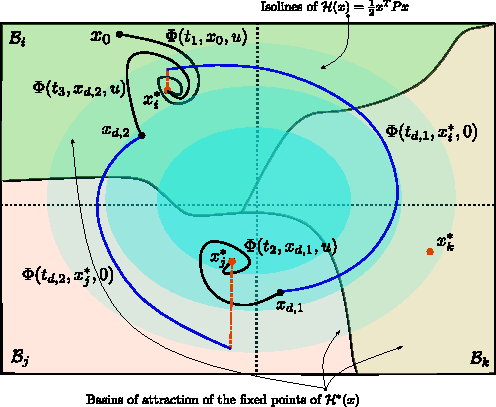
\includegraphics[scale = 1]{draw.pdf}
%    \caption{\footnotesize Graphical representation of a state-space trajectory of the controlled system.}
%    \label{fig:my_label}
%\end{figure}
%%%%
%\section{Case of Study}
%
\begin{figure}[h]
    \centering
    %\subfigure[{\footnotesize Time evolution of the states $x = [\xi,\dot{\xi}]^\top$.}]{%%
\definecolor{ocean}{rgb}{0.00000,0.44700,0.74100}
%
\begin{tikzpicture}

\begin{axis}[%
width=11cm,
height=2cm,
at={(0.758in,1.9in)},
scale only axis,
xmin=0,
xmax=17,
xlabel style={font=\color{white!15!black}},
xlabel={$t$ [$s$]},
ymin=-.8,
ymax=0.75,
ylabel style={font=\color{white!15!black}},
ylabel={$q(t)$ [m]},
axis background/.style={fill=white},
legend style={legend cell align=left, align=left, draw=white!15!black}
]
\addplot [color=ocean, dashed, line width=1.0pt,forget plot]
  table[row sep=crcr]{%
0	0.5\\
17.103	0.5\\
};
%\addlegendentry{data1}

\addplot [color=ocean, dashed, line width=1.0pt,forget plot]
  table[row sep=crcr]{%
0	-0.5\\
17.103	-0.5\\
};
%\addlegendentry{data2}

\addplot [color=black, line width=2pt]
  table[row sep=crcr]{%
0	-0.8\\
0.0201272951242755	-0.79951111951868\\
0.040254590248551	-0.79811008082095\\
0.0603818853728264	-0.795891468826249\\
0.0805091804971019	-0.792944776187467\\
0.141450272956506	-0.780417561508645\\
0.20239136541591	-0.764029602799776\\
0.263332457875313	-0.745456884813622\\
0.324273550334717	-0.725973531204578\\
0.406594062839508	-0.69990596289271\\
0.488914575344299	-0.675182591346937\\
0.571235087849089	-0.652469688739267\\
0.65355560035388	-0.632345559216368\\
0.723870856097015	-0.617338757000783\\
0.79418611184015	-0.604082781999283\\
0.864501367583285	-0.592424562970695\\
0.93481662332642	-0.582229375736837\\
1.0247788223884	-0.571064115086853\\
1.11474102145038	-0.561683876754374\\
1.20470322051236	-0.553799404485863\\
1.29466541957433	-0.547142777898694\\
1.41966541957433	-0.539436820468652\\
1.54466541957433	-0.533271711347302\\
1.66966541957433	-0.528402657479605\\
1.79466541957433	-0.524404342745406\\
1.91302238550665	-0.521127077977175\\
2.03137935143897	-0.518368646475493\\
2.14973631737129	-0.516056201969089\\
2.26809328330361	-0.514075304343261\\
2.39309328330361	-0.512245794028465\\
2.51809328330361	-0.510679923857475\\
2.64309328330361	-0.509344153381082\\
2.76809328330361	-0.508187986884424\\
2.89309328330361	-0.507171843510017\\
3.01809328330361	-0.506289351619222\\
3.14309328330361	-0.505524109227117\\
3.26809328330361	-0.504855709483334\\
3.39309328330361	-0.504267478547139\\
3.51809328330361	-0.503752835833422\\
3.64309328330361	-0.503302933885505\\
3.76809328330361	-0.502908156125825\\
3.89309328330361	-0.502560388348614\\
4.01809328330361	-0.502254970332233\\
4.14309328330361	-0.501986874345041\\
4.26809328330361	-0.501751052269233\\
4.39309328330361	-0.501543159535206\\
4.51809328330361	-0.501360211144487\\
4.64309328330361	-0.501199269031116\\
4.76809328330361	-0.501057509775478\\
4.82606996247771	-0.500997563859026\\
4.88404664165181	-0.500941038274212\\
4.9420233208259	-0.500887735750696\\
5	-0.500837469394745\\
};
%\addlegendentry{data3}

\addplot [color=gray, line width=2pt]
  table[row sep=crcr]{%
5	-0.500837469394745\\
5.001	-0.49979049724748\\
5.002	-0.498741550128628\\
5.003	-0.497690634268849\\
5.004	-0.496637755905533\\
5.005	-0.495582921282759\\
5.006	-0.494526136651266\\
5.007	-0.493467408268413\\
5.008	-0.492406742398151\\
5.009	-0.491344145310982\\
5.01	-0.490279623283929\\
5.011	-0.489213182600499\\
5.012	-0.488144829550648\\
5.013	-0.487074570430748\\
5.014	-0.486002411543552\\
5.015	-0.484928359198159\\
5.016	-0.483852419709978\\
5.017	-0.482774599400694\\
5.018	-0.481694904598237\\
5.019	-0.48061334163674\\
5.02	-0.47952991685651\\
5.021	-0.478444636603992\\
5.022	-0.477357507231732\\
5.023	-0.476268535098345\\
5.024	-0.475177726568479\\
5.025	-0.47408508801278\\
5.026	-0.472990625807857\\
5.027	-0.471894346336247\\
5.028	-0.470796255986381\\
5.029	-0.46969636115255\\
5.03	-0.468594668234867\\
5.031	-0.467491183639235\\
5.032	-0.46638591377731\\
5.033	-0.465278865066468\\
5.034	-0.464170043929769\\
5.035	-0.463059456795921\\
5.036	-0.461947110099249\\
5.037	-0.460833010279654\\
5.038	-0.459717163782583\\
5.039	-0.458599577058993\\
5.04	-0.457480256565313\\
5.041	-0.456359208763413\\
5.042	-0.455236440120568\\
5.043	-0.454111957109419\\
5.044	-0.452985766207944\\
5.045	-0.45185787389942\\
5.046	-0.450728286672388\\
5.047	-0.449597011020615\\
5.048	-0.448464053443067\\
5.049	-0.447329420443865\\
5.05	-0.446193118532255\\
5.051	-0.445055154222572\\
5.052	-0.443915534034204\\
5.053	-0.442774264491558\\
5.054	-0.441631352124023\\
5.055	-0.440486803465939\\
5.056	-0.439340625056556\\
5.057	-0.438192823440002\\
5.058	-0.437043405165252\\
5.059	-0.435892376786083\\
5.06	-0.434739744861047\\
5.061	-0.433585515953434\\
5.062	-0.432429696631236\\
5.063	-0.43127229346711\\
5.064	-0.430113313038346\\
5.065	-0.42895276192683\\
5.066	-0.427790646719011\\
5.067	-0.426626974005863\\
5.068	-0.42546175038285\\
5.069	-0.424294982449892\\
5.07	-0.423126676811331\\
5.071	-0.421956840075892\\
5.072	-0.420785478856653\\
5.073	-0.419612599771004\\
5.074	-0.418438209440616\\
5.075	-0.417262314491403\\
5.076	-0.416084921553491\\
5.077	-0.414906037261176\\
5.078	-0.413725668252895\\
5.079	-0.412543821171189\\
5.08	-0.411360502662664\\
5.081	-0.410175719377961\\
5.082	-0.40898947797172\\
5.083	-0.407801785102539\\
5.084	-0.406612647432948\\
5.085	-0.405422071629365\\
5.086	-0.404230064362065\\
5.087	-0.403036632305147\\
5.088	-0.401841782136493\\
5.089	-0.400645520537737\\
5.09	-0.399447854194227\\
5.091	-0.398248789794994\\
5.092	-0.39704833403271\\
5.093	-0.39584649360366\\
5.094	-0.394643275207702\\
5.095	-0.393438685548233\\
5.096	-0.392232731332152\\
5.097	-0.391025419269831\\
5.098	-0.389816756075069\\
5.099	-0.388606748465069\\
5.1	-0.387395403160393\\
5.101	-0.38618272688493\\
5.102	-0.384968726365864\\
5.103	-0.383753408333633\\
5.104	-0.382536779521899\\
5.105	-0.381318846667507\\
5.106	-0.380099616510457\\
5.107	-0.378879095793861\\
5.108	-0.377657291263914\\
5.109	-0.376434209669855\\
5.11	-0.375209857763933\\
5.111	-0.373984242301372\\
5.112	-0.372757370040337\\
5.113	-0.371529247741893\\
5.114	-0.370299882169979\\
5.115	-0.369069280091363\\
5.116	-0.367837448275615\\
5.117	-0.366604393495067\\
5.118	-0.365370122524777\\
5.119	-0.3641346421425\\
5.12	-0.362897959128645\\
5.121	-0.361660080266244\\
5.122	-0.360421012340917\\
5.123	-0.359180762140835\\
5.124	-0.357939336456686\\
5.125	-0.35669674208164\\
5.126	-0.355452985811312\\
5.127	-0.354208074443729\\
5.128	-0.352962014779294\\
5.129	-0.35171481362075\\
5.13	-0.350466477773145\\
5.131	-0.3492170140438\\
5.132	-0.347966429242268\\
5.133	-0.346714730180303\\
5.134	-0.345461923671826\\
5.135	-0.344208016532885\\
5.136	-0.342953015581624\\
5.137	-0.341696927638246\\
5.138	-0.340439759524977\\
5.139	-0.339181518066036\\
5.14	-0.337922210087593\\
5.141	-0.336661842417738\\
5.142	-0.335400421886444\\
5.143	-0.334137955325534\\
5.144	-0.332874449568645\\
5.145	-0.331609911451192\\
5.146	-0.330344347810333\\
5.147	-0.329077765484936\\
5.148	-0.327810171315542\\
5.149	-0.32654157214433\\
5.15	-0.325271974815084\\
5.151	-0.324001386173155\\
5.152	-0.322729813065428\\
5.153	-0.321457262340287\\
5.154	-0.320183740847578\\
5.155	-0.318909255438578\\
5.156	-0.317633812965955\\
5.157	-0.316357420283737\\
5.158	-0.315080084247277\\
5.159	-0.313801811713214\\
5.16	-0.312522609539442\\
5.161	-0.311242484585075\\
5.162	-0.30996144371041\\
5.163	-0.308679493776893\\
5.164	-0.307396641647085\\
5.165	-0.306112894184626\\
5.166	-0.3048282582542\\
5.167	-0.303542740721503\\
5.168	-0.302256348453202\\
5.169	-0.300969088316908\\
5.17	-0.299680967181136\\
5.171	-0.29839199191527\\
5.172	-0.297102169389532\\
5.173	-0.295811506474943\\
5.174	-0.294520010043293\\
5.175	-0.293227686967099\\
5.176	-0.29193454411958\\
5.177	-0.290640588374614\\
5.178	-0.289345826606706\\
5.179	-0.288050265690955\\
5.18	-0.286753912503019\\
5.181	-0.285456773919077\\
5.182	-0.284158856815798\\
5.183	-0.282860168070305\\
5.184	-0.281560714560141\\
5.185	-0.280260503163233\\
5.186	-0.27895954075786\\
5.187	-0.277657834222614\\
5.188	-0.276355390436372\\
5.189	-0.275052216278254\\
5.19	-0.273748318627596\\
5.191	-0.272443704363908\\
5.192	-0.271138380366845\\
5.193	-0.269832353516173\\
5.194	-0.268525630691728\\
5.195	-0.26721821877339\\
5.196	-0.265910124641041\\
5.197	-0.264601355174536\\
5.198	-0.263291917253668\\
5.199	-0.26198181775813\\
5.2	-0.260671063567484\\
5.201	-0.259359661561126\\
5.202	-0.258047618618251\\
5.203	-0.25673494161782\\
5.204	-0.255421637438523\\
5.205	-0.25410771295875\\
5.206	-0.252793175056549\\
5.207	-0.251478030609599\\
5.208	-0.250162286495173\\
5.209	-0.248845949590103\\
5.21	-0.247529026770747\\
5.211	-0.246211524912954\\
5.212	-0.244893450892031\\
5.213	-0.243574811582708\\
5.214	-0.242255613859104\\
5.215	-0.240935864594694\\
5.216	-0.239615570662274\\
5.217	-0.238294738933926\\
5.218	-0.236973376280986\\
5.219	-0.23565148957401\\
5.22	-0.234329085682737\\
5.221	-0.233006171476058\\
5.222	-0.231682753821984\\
5.223	-0.230358839587605\\
5.224	-0.229034435639065\\
5.225	-0.22770954884152\\
5.226	-0.22638418605911\\
5.227	-0.225058354154922\\
5.228	-0.22373205999096\\
5.229	-0.222405310428105\\
5.23	-0.221078112326087\\
5.231	-0.219750472543448\\
5.232	-0.21842239793751\\
5.233	-0.217093895364341\\
5.234	-0.215764971678721\\
5.235	-0.214435633734109\\
5.236	-0.213105888382607\\
5.237	-0.21177574247493\\
5.238	-0.210445202860371\\
5.239	-0.209114276386766\\
5.24	-0.207782969900463\\
5.241	-0.206451290246286\\
5.242	-0.205119244267504\\
5.243	-0.203786838805796\\
5.244	-0.202454080701216\\
5.245	-0.201120976792166\\
5.246	-0.199787533915354\\
5.247	-0.198453758905768\\
5.248	-0.197119658596637\\
5.249	-0.195785239819401\\
5.25	-0.19445050940368\\
5.251	-0.193115474177233\\
5.252	-0.191780140965933\\
5.253	-0.19044451659373\\
5.254	-0.189108607882618\\
5.255	-0.187772421652601\\
5.256	-0.186435964721663\\
5.257	-0.185099243905732\\
5.258	-0.183762266018648\\
5.259	-0.182425037872131\\
5.26	-0.181087566275745\\
5.261	-0.179749858036868\\
5.262	-0.17841191996066\\
5.263	-0.177073758850025\\
5.264	-0.175735381505582\\
5.265	-0.174396794725634\\
5.266	-0.17305800530613\\
5.267	-0.171719020040634\\
5.268	-0.170379845720297\\
5.269	-0.169040489133817\\
5.27	-0.16770095706741\\
5.271	-0.166361256304778\\
5.272	-0.165021393627074\\
5.273	-0.163681375812872\\
5.274	-0.162341209638133\\
5.275	-0.16100090187617\\
5.276	-0.159660459297622\\
5.277	-0.158319888670414\\
5.278	-0.156979196759729\\
5.279	-0.155638390327976\\
5.28	-0.154297476134753\\
5.281	-0.152956460936822\\
5.282	-0.151615351488068\\
5.283	-0.150274154539473\\
5.284	-0.148932876839083\\
5.285	-0.147591525131972\\
5.286	-0.146250106160215\\
5.287	-0.144908626662849\\
5.288	-0.14356709337585\\
5.289	-0.142225513032091\\
5.29	-0.140883892361318\\
5.291	-0.139542238090113\\
5.292	-0.138200556941864\\
5.293	-0.136858855636731\\
5.294	-0.135517140891619\\
5.295	-0.134175419420138\\
5.296	-0.13283369793258\\
5.297	-0.13149198313588\\
5.298	-0.130150281733587\\
5.299	-0.128808600425834\\
5.3	-0.127466945909303\\
5.301	-0.126125324877194\\
5.302	-0.124783744019195\\
5.303	-0.123442210021449\\
5.304	-0.122100729566522\\
5.305	-0.120759309333373\\
5.306	-0.119417955997319\\
5.307	-0.118076676230009\\
5.308	-0.116735476699386\\
5.309	-0.115394364069661\\
5.31	-0.114053345001279\\
5.311	-0.112712426150887\\
5.312	-0.111371614171304\\
5.313	-0.11003091571149\\
5.314	-0.108690337416512\\
5.315	-0.107349885927518\\
5.316	-0.106009567881698\\
5.317	-0.104669389912261\\
5.318	-0.103329358648398\\
5.319	-0.101989480715252\\
5.32	-0.100649762733891\\
5.321	-0.0993102113212709\\
5.322	-0.0979708330902083\\
5.323	-0.0966316346493487\\
5.324	-0.095292622603135\\
5.325	-0.0939538035517772\\
5.326	-0.0926151840912212\\
5.327	-0.091276770813118\\
5.328	-0.089938570304793\\
5.329	-0.0886005891492154\\
5.33	-0.0872628339249669\\
5.331	-0.0859253112062114\\
5.332	-0.0845880275626645\\
5.333	-0.0832509895595626\\
5.334	-0.0819142037576322\\
5.335	-0.0805776767130602\\
5.336	-0.0792414149774617\\
5.337	-0.0779054250978517\\
5.338	-0.0765697136166129\\
5.339	-0.075234287071466\\
5.34	-0.07389915199544\\
5.341	-0.0725643149168403\\
5.342	-0.07122978235922\\
5.343	-0.0698955608413485\\
5.344	-0.0685616568771824\\
5.345	-0.0672280769758344\\
5.346	-0.0658948276415436\\
5.347	-0.0645619153736455\\
5.348	-0.0632293466665414\\
5.349	-0.0618971280096696\\
5.35	-0.060565265887474\\
5.351	-0.0592337667793751\\
5.352	-0.05790263715974\\
5.353	-0.0565718834978522\\
5.354	-0.0552415122578822\\
5.355	-0.0539115298988578\\
5.356	-0.0525819428746338\\
5.357	-0.0512527576338628\\
5.358	-0.0499239806199655\\
5.359	-0.0485956182711013\\
5.36	-0.047267677020138\\
5.361	-0.0459401632946234\\
5.362	-0.0446130835167548\\
5.363	-0.0432864441033503\\
5.364	-0.0419602514658187\\
5.365	-0.0406345120101312\\
5.366	-0.039309232136791\\
5.367	-0.0379844182408046\\
5.368	-0.0366600767116525\\
5.369	-0.0353362139332602\\
5.37	-0.0340128362839687\\
5.371	-0.0326899501365054\\
5.372	-0.0313675618579557\\
5.373	-0.0300456778097334\\
5.374	-0.0287243043475516\\
5.375	-0.0274034478213942\\
5.376	-0.0260831145754869\\
5.377	-0.0247633109482682\\
5.378	-0.0234440432723611\\
5.379	-0.0221253178745435\\
5.38	-0.0208071410757205\\
5.381	-0.0194895191908947\\
5.382	-0.0181724585291384\\
5.383	-0.016855965393565\\
5.384	-0.0155400460812999\\
5.385	-0.0142247068834518\\
5.386	-0.0129099540850861\\
5.387	-0.0115957939651936\\
5.388	-0.0102822327966659\\
5.389	-0.00896927684626214\\
5.39	-0.00765693237458575\\
5.391	-0.0063452056360531\\
5.392	-0.00503410287886636\\
5.393	-0.00372363034498555\\
5.394	-0.00241379427009969\\
5.395	-0.0011046008835993\\
5.396	0.000203943591451302\\
5.397	0.0015118329383424\\
5.398	0.00281906094674719\\
5.399	0.00412562141274814\\
5.4	0.00543150813886684\\
5.401	0.00673671493408997\\
5.402	0.00804123561389757\\
5.403	0.00934506400029216\\
5.404	0.0106481939218239\\
5.405	0.0119506192136194\\
5.406	0.0132523337174095\\
5.407	0.0145533312815565\\
5.408	0.0158536057610819\\
5.409	0.0171531510176924\\
5.41	0.0184519609198095\\
5.411	0.0197500293425944\\
5.412	0.0210473501679772\\
5.413	0.0223439172846833\\
5.414	0.0236397245882604\\
5.415	0.0249347659811057\\
5.416	0.0262290353724928\\
5.417	0.0275225266785995\\
5.418	0.0288152338225342\\
5.419	0.0301071507343621\\
5.42	0.0313982713511336\\
5.421	0.0326885896169101\\
5.422	0.0339780994827902\\
5.423	0.0352667949069385\\
5.424	0.0365546698546095\\
5.425	0.0378417182981771\\
5.426	0.0391279342171583\\
5.427	0.0404133115982428\\
5.428	0.0416978444353165\\
5.429	0.0429815267294897\\
5.43	0.0442643524891232\\
5.431	0.0455463157298544\\
5.432	0.0468274104746235\\
5.433	0.0481076307537001\\
5.434	0.049386970604709\\
5.435	0.0506654240726563\\
5.436	0.0519429852099562\\
5.437	0.0532196480764561\\
5.438	0.0544954067394627\\
5.439	0.055770255273769\\
5.44	0.0570441877616786\\
5.441	0.0583171982930327\\
5.442	0.0595892809652352\\
5.443	0.0608604298832792\\
5.444	0.0621306391597711\\
5.445	0.0633999029149586\\
5.446	0.064668215276754\\
5.447	0.0659355703807614\\
5.448	0.0672019623703011\\
5.449	0.0684673853964348\\
5.45	0.0697318336179926\\
5.451	0.0709953012015971\\
5.452	0.0722577823216878\\
5.453	0.0735192711605486\\
5.454	0.0747797619083308\\
5.455	0.0760392487630796\\
5.456	0.0772977259307582\\
5.457	0.078555187625274\\
5.458	0.0798116280685019\\
5.459	0.0810670414903111\\
5.46	0.0823214221285883\\
5.461	0.0835747642292631\\
5.462	0.0848270620463332\\
5.463	0.0860783098418888\\
5.464	0.087328501886136\\
5.465	0.0885776324574246\\
5.466	0.0898256958422682\\
5.467	0.0910726863353727\\
5.468	0.0923185982396584\\
5.469	0.093563425866285\\
5.47	0.0948071635346761\\
5.471	0.0960498055725434\\
5.472	0.0972913463159107\\
5.473	0.0985317801091379\\
5.474	0.0997711013049459\\
5.475	0.10100930426444\\
5.476	0.102246383357133\\
5.477	0.103482332960971\\
5.478	0.104717147462358\\
5.479	0.105950821256176\\
5.48	0.107183348745811\\
5.481	0.108414724343178\\
5.482	0.109644942468743\\
5.483	0.110873997551545\\
5.484	0.112101884029226\\
5.485	0.113328596348044\\
5.486	0.114554128962909\\
5.487	0.115778476337395\\
5.488	0.11700163294377\\
5.489	0.118223593263017\\
5.49	0.119444351784859\\
5.491	0.12066390300778\\
5.492	0.121882241439049\\
5.493	0.123099361594743\\
5.494	0.124315257999771\\
5.495	0.125529925187896\\
5.496	0.126743357701756\\
5.497	0.127955550092892\\
5.498	0.129166496921764\\
5.499	0.13037619275778\\
5.5	0.131584632179317\\
5.501	0.132791809773739\\
5.502	0.133997720137426\\
5.503	0.135202357875792\\
5.504	0.13640571760331\\
5.505	0.137607793943535\\
5.506	0.138808581529122\\
5.507	0.140008075001852\\
5.508	0.141206269012656\\
5.509	0.142403158221631\\
5.51	0.143598737298068\\
5.511	0.14479300092047\\
5.512	0.145985943776576\\
5.513	0.147177560563385\\
5.514	0.148367845987173\\
5.515	0.149556794763518\\
5.516	0.150744401617321\\
5.517	0.151930661282828\\
5.518	0.153115568503652\\
5.519	0.154299118032793\\
5.52	0.155481304632662\\
5.521	0.156662123075099\\
5.522	0.157841568141399\\
5.523	0.159019634622329\\
5.524	0.160196317318151\\
5.525	0.161371611038646\\
5.526	0.162545510603129\\
5.527	0.163718010840477\\
5.528	0.164889106589144\\
5.529	0.166058792697187\\
5.53	0.167227064022284\\
5.531	0.168393915431755\\
5.532	0.169559341802584\\
5.533	0.17072333802144\\
5.534	0.171885898984696\\
5.535	0.17304701959845\\
5.536	0.174206694778549\\
5.537	0.175364919450605\\
5.538	0.176521688550015\\
5.539	0.177676997021988\\
5.54	0.17883083982156\\
5.541	0.179983211913612\\
5.542	0.181134108272897\\
5.543	0.182283523884057\\
5.544	0.18343145374164\\
5.545	0.184577892850127\\
5.546	0.185722836223945\\
5.547	0.18686627888749\\
5.548	0.188008215875149\\
5.549	0.189148642231316\\
5.55	0.190287553010413\\
5.551	0.191424943276912\\
5.552	0.192560808105351\\
5.553	0.193695142580358\\
5.554	0.194827941796663\\
5.555	0.195959200859129\\
5.556	0.197088914882758\\
5.557	0.198217078992723\\
5.558	0.199343688324378\\
5.559	0.200468738023281\\
5.56	0.201592223245215\\
5.561	0.202714139156201\\
5.562	0.203834480932525\\
5.563	0.204953243760751\\
5.564	0.206070422837742\\
5.565	0.207186013370678\\
5.566	0.208300010577077\\
5.567	0.209412409684812\\
5.568	0.21052320593213\\
5.569	0.21163239456767\\
5.57	0.212739970850481\\
5.571	0.213845930050045\\
5.572	0.214950267446289\\
5.573	0.216052978329608\\
5.574	0.217154058000879\\
5.575	0.218253501771488\\
5.576	0.219351304963335\\
5.577	0.220447462908865\\
5.578	0.221541970951076\\
5.579	0.222634824443546\\
5.58	0.223726018750442\\
5.581	0.224815549246543\\
5.582	0.225903411317261\\
5.583	0.226989600358649\\
5.584	0.228074111777428\\
5.585	0.229156940991\\
5.586	0.230238083427467\\
5.587	0.231317534525649\\
5.588	0.232395289735098\\
5.589	0.23347134451612\\
5.59	0.234545694339791\\
5.591	0.235618334687971\\
5.592	0.236689261053326\\
5.593	0.237758468939342\\
5.594	0.238825953860342\\
5.595	0.239891711341507\\
5.596	0.240955736918885\\
5.597	0.242018026139418\\
5.598	0.24307857456095\\
5.599	0.244137377752249\\
5.6	0.245194431293021\\
5.601	0.246249730773929\\
5.602	0.247303271796606\\
5.603	0.248355049973677\\
5.604	0.249405060928769\\
5.605	0.250453300296532\\
5.606	0.251499763722653\\
5.607	0.252544446863876\\
5.608	0.253587345388011\\
5.609	0.254628454973957\\
5.61	0.255667771311715\\
5.611	0.256705290102405\\
5.612	0.25774100705828\\
5.613	0.258774917902744\\
5.614	0.259807018370367\\
5.615	0.260837304206902\\
5.616	0.261865771169297\\
5.617	0.262892415025715\\
5.618	0.263917231555547\\
5.619	0.264940216549428\\
5.62	0.265961365809254\\
5.621	0.266980675148193\\
5.622	0.267998140390705\\
5.623	0.269013757372557\\
5.624	0.270027521940833\\
5.625	0.271039429953955\\
5.626	0.272049477281696\\
5.627	0.273057659805193\\
5.628	0.274063973416965\\
5.629	0.275068414020926\\
5.63	0.2760709775324\\
5.631	0.277071659878137\\
5.632	0.278070456996324\\
5.633	0.279067364836606\\
5.634	0.280062379360093\\
5.635	0.281055496539382\\
5.636	0.282046712358562\\
5.637	0.28303602281324\\
5.638	0.284023423910545\\
5.639	0.285008911669149\\
5.64	0.285992482119275\\
5.641	0.286974131302718\\
5.642	0.287953855272855\\
5.643	0.288931650094657\\
5.644	0.289907511844708\\
5.645	0.290881436611215\\
5.646	0.291853420494023\\
5.647	0.292823459604628\\
5.648	0.293791550066194\\
5.649	0.294757688013559\\
5.65	0.295721869593257\\
5.651	0.296684090963527\\
5.652	0.297644348294326\\
5.653	0.298602637767343\\
5.654	0.299558955576015\\
5.655	0.300513297925534\\
5.656	0.301465661032867\\
5.657	0.302416041126763\\
5.658	0.303364434447772\\
5.659	0.304310837248251\\
5.66	0.305255245792384\\
5.661	0.306197656356188\\
5.662	0.307138065227531\\
5.663	0.308076468706143\\
5.664	0.309012863103625\\
5.665	0.309947244743469\\
5.666	0.310879609961062\\
5.667	0.311809955103704\\
5.668	0.312738276530621\\
5.669	0.313664570612971\\
5.67	0.314588833733864\\
5.671	0.315511062288367\\
5.672	0.31643125268352\\
5.673	0.31734940133835\\
5.674	0.318265504683876\\
5.675	0.319179559163128\\
5.676	0.320091561231156\\
5.677	0.321001507355039\\
5.678	0.321909394013901\\
5.679	0.322815217698921\\
5.68	0.323718974913344\\
5.681	0.32462066217249\\
5.682	0.325520276003773\\
5.683	0.326417812946704\\
5.684	0.327313269552906\\
5.685	0.328206642386125\\
5.686	0.329097928022243\\
5.687	0.329987123049284\\
5.688	0.330874224067429\\
5.689	0.331759227689028\\
5.69	0.332642130538605\\
5.691	0.333522929252875\\
5.692	0.334401620480752\\
5.693	0.335278200883359\\
5.694	0.336152667134042\\
5.695	0.337025015918374\\
5.696	0.337895243934174\\
5.697	0.338763347891508\\
5.698	0.339629324512709\\
5.699	0.340493170532378\\
5.7	0.341354882697402\\
5.701	0.34221445776696\\
5.702	0.343071892512534\\
5.703	0.343927183717916\\
5.704	0.344780328179224\\
5.705	0.345631322704907\\
5.706	0.346480164115758\\
5.707	0.34732684924492\\
5.708	0.348171374937899\\
5.709	0.349013738052571\\
5.71	0.349853935459196\\
5.711	0.35069196404042\\
5.712	0.351527820691292\\
5.713	0.352361502319268\\
5.714	0.353193005844223\\
5.715	0.354022328198461\\
5.716	0.354849466326721\\
5.717	0.355674417186187\\
5.718	0.356497177746498\\
5.719	0.357317744989758\\
5.72	0.358136115910543\\
5.721	0.358952287515908\\
5.722	0.359766256825401\\
5.723	0.360578020871066\\
5.724	0.361387576697456\\
5.725	0.362194921361639\\
5.726	0.363000051933207\\
5.727	0.363802965494285\\
5.728	0.364603659139537\\
5.729	0.36540212997618\\
5.73	0.366198375123984\\
5.731	0.366992391715286\\
5.732	0.367784176894999\\
5.733	0.368573727820614\\
5.734	0.369361041662212\\
5.735	0.370146115602472\\
5.736	0.370928946836679\\
5.737	0.371709532572729\\
5.738	0.372487870031138\\
5.739	0.373263956445052\\
5.74	0.374037789060251\\
5.741	0.374809365135159\\
5.742	0.375578681940848\\
5.743	0.376345736761051\\
5.744	0.377110526892164\\
5.745	0.377873049643254\\
5.746	0.37863330233607\\
5.747	0.379391282305045\\
5.748	0.380146986897306\\
5.749	0.38090041347268\\
5.75	0.381651559403701\\
5.751	0.382400422075617\\
5.752	0.383146998886396\\
5.753	0.383891287246733\\
5.754	0.384633284580059\\
5.755	0.385372988322542\\
5.756	0.386110395923098\\
5.757	0.386845504843397\\
5.758	0.387578312557867\\
5.759	0.388308816553701\\
5.76	0.389037014330867\\
5.761	0.389762903402108\\
5.762	0.390486481292951\\
5.763	0.391207745541714\\
5.764	0.391926693699512\\
5.765	0.392643323330258\\
5.766	0.393357632010677\\
5.767	0.394069617330303\\
5.768	0.394779276891492\\
5.769	0.395486608309423\\
5.77	0.396191609212105\\
5.771	0.396894277240381\\
5.772	0.397594610047939\\
5.773	0.398292605301307\\
5.774	0.398988260679869\\
5.775	0.399681573875865\\
5.776	0.400372542594394\\
5.777	0.401061164553424\\
5.778	0.401747437483793\\
5.779	0.402431359129217\\
5.78	0.403112927246292\\
5.781	0.4037921396045\\
5.782	0.404468993986216\\
5.783	0.405143488186709\\
5.784	0.405815620014147\\
5.785	0.406485387289603\\
5.786	0.407152787847061\\
5.787	0.407817819533417\\
5.788	0.408480480208483\\
5.789	0.409140767744997\\
5.79	0.409798680028617\\
5.791	0.410454214957939\\
5.792	0.411107370444486\\
5.793	0.411758144412723\\
5.794	0.412406534800056\\
5.795	0.413052539556839\\
5.796	0.413696156646372\\
5.797	0.414337384044912\\
5.798	0.414976219741671\\
5.799	0.415612661738822\\
5.8	0.416246708051503\\
5.801	0.416878356707818\\
5.802	0.417507605748843\\
5.803	0.41813445322863\\
5.804	0.418758897214206\\
5.805	0.419380935785579\\
5.806	0.420000567035741\\
5.807	0.420617789070672\\
5.808	0.42123260000934\\
5.809	0.421844997983709\\
5.81	0.422454981138734\\
5.811	0.423062547632372\\
5.812	0.423667695635579\\
5.813	0.424270423332316\\
5.814	0.424870728919549\\
5.815	0.425468610607256\\
5.816	0.426064066618421\\
5.817	0.426657095189046\\
5.818	0.427247694568147\\
5.819	0.427835863017759\\
5.82	0.428421598812936\\
5.821	0.429004900241757\\
5.822	0.429585765605322\\
5.823	0.430164193217762\\
5.824	0.430740181406232\\
5.825	0.43131372851092\\
5.826	0.431884832885046\\
5.827	0.432453492894861\\
5.828	0.433019706919656\\
5.829	0.433583473351754\\
5.83	0.434144790596522\\
5.831	0.434703657072361\\
5.832	0.435260071210718\\
5.833	0.435814031456081\\
5.834	0.436365536265983\\
5.835	0.436914584110999\\
5.836	0.437461173474754\\
5.837	0.438005302853919\\
5.838	0.438546970758212\\
5.839	0.439086175710403\\
5.84	0.439622916246309\\
5.841	0.440157190914799\\
5.842	0.440688998277796\\
5.843	0.441218336910272\\
5.844	0.441745205400254\\
5.845	0.44226960234882\\
5.846	0.442791526370106\\
5.847	0.443310976091298\\
5.848	0.443827950152639\\
5.849	0.444342447207426\\
5.85	0.444854465922012\\
5.851	0.445364004975806\\
5.852	0.445871063061268\\
5.853	0.44637563888392\\
5.854	0.446877731162333\\
5.855	0.447377338628137\\
5.856	0.447874460026016\\
5.857	0.448369094113709\\
5.858	0.448861239662007\\
5.859	0.449350895454759\\
5.86	0.449838060288865\\
5.861	0.450322732974279\\
5.862	0.450804912334007\\
5.863	0.451284597204107\\
5.864	0.451761786433688\\
5.865	0.45223647888491\\
5.866	0.452708673432982\\
5.867	0.453178368966162\\
5.868	0.453645564385755\\
5.869	0.454110258606113\\
5.87	0.454572450554634\\
5.871	0.45503213917176\\
5.872	0.455489323410976\\
5.873	0.455944002238809\\
5.874	0.456396174634828\\
5.875	0.456845839591638\\
5.876	0.457292996114884\\
5.877	0.457737643223247\\
5.878	0.458179779948441\\
5.879	0.458619405335215\\
5.88	0.459056518441345\\
5.881	0.459491118337643\\
5.882	0.459923204107941\\
5.883	0.460352774849102\\
5.884	0.460779829671009\\
5.885	0.461204367696568\\
5.886	0.461626388061704\\
5.887	0.46204588991536\\
5.888	0.462462872419491\\
5.889	0.462877334749068\\
5.89	0.46328927609207\\
5.891	0.463698695649484\\
5.892	0.464105592635303\\
5.893	0.464509966276521\\
5.894	0.464911815813134\\
5.895	0.465311140498133\\
5.896	0.465707939597506\\
5.897	0.46610221239023\\
5.898	0.466493958168274\\
5.899	0.46688317623659\\
5.9	0.467269865913114\\
5.901	0.467654026528761\\
5.902	0.468035657427424\\
5.903	0.468414757965968\\
5.904	0.46879132751423\\
5.905	0.469165365455011\\
5.906	0.469536871184078\\
5.907	0.469905844110155\\
5.908	0.470272283654926\\
5.909	0.470636189253026\\
5.91	0.470997560352039\\
5.911	0.471356396412494\\
5.912	0.471712696907862\\
5.913	0.472066461324554\\
5.914	0.472417689161912\\
5.915	0.472766379932209\\
5.916	0.473112533160645\\
5.917	0.47345614838534\\
5.918	0.473797225157333\\
5.919	0.474135763040577\\
5.92	0.474471761611933\\
5.921	0.474805220461166\\
5.922	0.475136139190945\\
5.923	0.475464517416832\\
5.924	0.475790354767281\\
5.925	0.476113650883633\\
5.926	0.476434405420113\\
5.927	0.476752618043821\\
5.928	0.477068288434732\\
5.929	0.477381416285687\\
5.93	0.47769200130239\\
5.931	0.478000043203407\\
5.932	0.478305541720151\\
5.933	0.478608496596888\\
5.934	0.478908907590725\\
5.935	0.479206774471605\\
5.936	0.479502097022307\\
5.937	0.479794875038434\\
5.938	0.480085108328412\\
5.939	0.480372796713482\\
5.94	0.480657940027698\\
5.941	0.480940538117917\\
5.942	0.481220590843797\\
5.943	0.481498098077788\\
5.944	0.481773059705129\\
5.945	0.482045475623841\\
5.946	0.482315345744724\\
5.947	0.482582669991343\\
5.948	0.482847448300032\\
5.949	0.483109680619882\\
5.95	0.483369366912735\\
5.951	0.48362650715318\\
5.952	0.483881101328545\\
5.953	0.484133149438894\\
5.954	0.484382651497015\\
5.955	0.484629607528419\\
5.956	0.484874017571329\\
5.957	0.485115881676677\\
5.958	0.485355199908096\\
5.959	0.485591972341914\\
5.96	0.485826199067145\\
5.961	0.486057880185485\\
5.962	0.486287015811303\\
5.963	0.486513606071637\\
5.964	0.486737651106184\\
5.965	0.486959151067293\\
5.966	0.487178106119961\\
5.967	0.487394516441822\\
5.968	0.487608382223145\\
5.969	0.487819703666818\\
5.97	0.488028480988351\\
5.971	0.488234714415862\\
5.972	0.48843840419007\\
5.973	0.488639550564291\\
5.974	0.488838153804427\\
5.975	0.489034214188958\\
5.976	0.48922773200894\\
5.977	0.489418707567988\\
5.978	0.489607141182279\\
5.979	0.489793033180533\\
5.98	0.489976383904014\\
5.981	0.490157193706518\\
5.982	0.490335462954364\\
5.983	0.490511192026391\\
5.984	0.490684381313942\\
5.985	0.490855031220863\\
5.986	0.491023142163492\\
5.987	0.491188714570647\\
5.988	0.491351748883626\\
5.989	0.491512245556191\\
5.99	0.491670205054563\\
5.991	0.49182562785741\\
5.992	0.491978514455846\\
5.993	0.492128865353413\\
5.994	0.492276681066079\\
5.995	0.492421962122226\\
5.996	0.492564709062641\\
5.997	0.492704922440511\\
5.998	0.492842602821408\\
5.999	0.492977750783285\\
6	0.493110366916464\\
6.001	0.493240451823628\\
6.002	0.493368006119813\\
6.003	0.493493030432395\\
6.004	0.493615525401086\\
6.005	0.493735491677919\\
6.006	0.493852929927244\\
6.007	0.493967840825714\\
6.008	0.494080225062277\\
6.009	0.494190083338169\\
6.01	0.494297416366901\\
6.011	0.494402224874248\\
6.012	0.494504509598247\\
6.013	0.494604271289176\\
6.014	0.494701510709554\\
6.015	0.494796228634126\\
6.016	0.494888425849852\\
6.017	0.494978103155902\\
6.018	0.495065261363642\\
6.019	0.495149901296623\\
6.02	0.495232023790576\\
6.021	0.495311629693394\\
6.022	0.49538871986513\\
6.023	0.49546329517798\\
6.024	0.495535356516275\\
6.025	0.495604904776473\\
6.026	0.495671940867145\\
6.027	0.495736465708963\\
6.028	0.495798480234697\\
6.029	0.495857985389194\\
6.03	0.495914982129376\\
6.031	0.495969471424225\\
6.032	0.49602145425477\\
6.033	0.496070931614082\\
6.034	0.496117904507258\\
6.035	0.496162373951413\\
6.036	0.496204340975667\\
6.037	0.496243806621135\\
6.038	0.496280771940915\\
6.039	0.496315238000075\\
6.04	0.496347205875648\\
6.041	0.496376676656614\\
6.042	0.496403651443891\\
6.043	0.496428131350323\\
6.044	0.49645011750067\\
6.045	0.496469611031596\\
6.046	0.496486613091655\\
6.047	0.496501124841282\\
6.048	0.496513147452781\\
6.049	0.496522682110312\\
6.05	0.496529730009879\\
6.051	0.49653429235932\\
};
%\addlegendentry{data4}

\addplot [color=black, line width=2pt]
  table[row sep=crcr]{%
6.051	0.49653429235932\\
6.176	0.496926194960609\\
6.301	0.497276850121281\\
6.426	0.497591075529191\\
6.551	0.497870227769207\\
6.676	0.498116271932668\\
6.801	0.498334587715316\\
6.926	0.498528372737258\\
7.051	0.498699911226424\\
7.176	0.498851373307831\\
7.301	0.498985372191164\\
7.426	0.499103923187673\\
7.551	0.499208710275864\\
7.676	0.499301255013317\\
7.801	0.499383029974462\\
7.926	0.499455280979485\\
8.051	0.499519098936501\\
8.176	0.499575456191341\\
8.301	0.499625225814305\\
8.426	0.49966917132255\\
8.551	0.499707973175075\\
8.676	0.499742234944969\\
8.801	0.499772482372023\\
8.926	0.499799181334092\\
9.051	0.499822750325593\\
9.176	0.499843559781005\\
9.301	0.499861927783756\\
9.426	0.499878137907887\\
9.551	0.499892445919136\\
9.676	0.49990507797607\\
9.801	0.499916226816221\\
9.926	0.499926064803327\\
10.051	0.49993474774883\\
10.176	0.499942413349355\\
10.301	0.499949178453657\\
10.426	0.499955147740769\\
10.551	0.499960415961223\\
10.676	0.499965066822313\\
10.801	0.499969171180145\\
10.926	0.499972792575672\\
11.051	0.499975988567965\\
};

%\addlegendentry{data5}

\addplot [color=gray, line width=2pt]
  table[row sep=crcr]{%
11.051	0.499975988567965\\
11.052	0.498930526268579\\
11.053	0.497883092541648\\
11.054	0.496833693608498\\
11.055	0.495782335697166\\
11.056	0.494729025042372\\
11.057	0.493673767885476\\
11.058	0.492616570474452\\
11.059	0.491557439063847\\
11.06	0.490496379914751\\
11.061	0.48943339929476\\
11.062	0.488368503477941\\
11.063	0.487301698744799\\
11.064	0.486232991382243\\
11.065	0.485162387683547\\
11.066	0.484089893948321\\
11.067	0.483015516482474\\
11.068	0.481939261598178\\
11.069	0.480861135613833\\
11.07	0.479781144854037\\
11.071	0.478699295649546\\
11.072	0.477615594337242\\
11.073	0.476530047260098\\
11.074	0.47544266076714\\
11.075	0.474353441213419\\
11.076	0.47326239495997\\
11.077	0.47216952837378\\
11.078	0.471074847827753\\
11.079	0.469978359700674\\
11.08	0.468880070377175\\
11.081	0.467779986247703\\
11.082	0.466678113708478\\
11.083	0.465574459161465\\
11.084	0.464469029014337\\
11.085	0.463361829680439\\
11.086	0.462252867578753\\
11.087	0.461142149133866\\
11.088	0.46002968077593\\
11.089	0.458915468940634\\
11.09	0.457799520069163\\
11.091	0.456681840608164\\
11.092	0.455562437009714\\
11.093	0.454441315731283\\
11.094	0.453318483235699\\
11.095	0.452193945991114\\
11.096	0.451067710470968\\
11.097	0.449939783153953\\
11.098	0.448810170523982\\
11.099	0.44767887907015\\
11.1	0.446545915286699\\
11.101	0.445411285672986\\
11.102	0.444274996733445\\
11.103	0.443137054977554\\
11.104	0.4419974669198\\
11.105	0.44085623907964\\
11.106	0.439713377981472\\
11.107	0.438568890154595\\
11.108	0.437422782133177\\
11.109	0.436275060456218\\
11.11	0.435125731667516\\
11.111	0.43397480231563\\
11.112	0.432822278953848\\
11.113	0.43166816814015\\
11.114	0.430512476437173\\
11.115	0.429355210412175\\
11.116	0.428196376637003\\
11.117	0.427035981688053\\
11.118	0.425874032146239\\
11.119	0.424710534596957\\
11.12	0.423545495630048\\
11.121	0.422378921839764\\
11.122	0.421210819824734\\
11.123	0.420041196187927\\
11.124	0.418870057536618\\
11.125	0.417697410482352\\
11.126	0.416523261640909\\
11.127	0.415347617632269\\
11.128	0.414170485080577\\
11.129	0.412991870614108\\
11.13	0.411811780865231\\
11.131	0.410630222470374\\
11.132	0.40944720206999\\
11.133	0.408262726308519\\
11.134	0.407076801834356\\
11.135	0.405889435299814\\
11.136	0.404700633361089\\
11.137	0.403510402678226\\
11.138	0.402318749915082\\
11.139	0.40112568173929\\
11.14	0.399931204822228\\
11.141	0.398735325838979\\
11.142	0.397538051468299\\
11.143	0.396339388392581\\
11.144	0.395139343297817\\
11.145	0.393937922873569\\
11.146	0.392735133812927\\
11.147	0.391530982812478\\
11.148	0.390325476572268\\
11.149	0.389118621795772\\
11.15	0.38791042518985\\
11.151	0.386700893464722\\
11.152	0.385490033333923\\
11.153	0.384277851514276\\
11.154	0.383064354725851\\
11.155	0.381849549691934\\
11.156	0.380633443138987\\
11.157	0.379416041796619\\
11.158	0.378197352397544\\
11.159	0.376977381677551\\
11.16	0.375756136375468\\
11.161	0.374533623233123\\
11.162	0.373309848995313\\
11.163	0.372084820409769\\
11.164	0.370858544227115\\
11.165	0.369631027200841\\
11.166	0.368402276087262\\
11.167	0.367172297645484\\
11.168	0.365941098637371\\
11.169	0.364708685827507\\
11.17	0.363475065983162\\
11.171	0.362240245874258\\
11.172	0.361004232273331\\
11.173	0.3597670319555\\
11.174	0.358528651698426\\
11.175	0.357289098282284\\
11.176	0.356048378489721\\
11.177	0.354806499105826\\
11.178	0.353563466918091\\
11.179	0.35231928871638\\
11.18	0.351073971292889\\
11.181	0.349827521442115\\
11.182	0.348579945960819\\
11.183	0.347331251647992\\
11.184	0.346081445304817\\
11.185	0.344830533734638\\
11.186	0.343578523742922\\
11.187	0.342325422137225\\
11.188	0.341071235727157\\
11.189	0.339815971324347\\
11.19	0.338559635742406\\
11.191	0.337302235796896\\
11.192	0.336043778305292\\
11.193	0.334784270086945\\
11.194	0.333523717963052\\
11.195	0.332262128756619\\
11.196	0.330999509292423\\
11.197	0.329735866396982\\
11.198	0.328471206898515\\
11.199	0.327205537626912\\
11.2	0.325938865413694\\
11.201	0.324671197091983\\
11.202	0.323402539496463\\
11.203	0.322132899463346\\
11.204	0.32086228383034\\
11.205	0.319590699436611\\
11.206	0.318318153122747\\
11.207	0.317044651730726\\
11.208	0.315770202103883\\
11.209	0.314494811086867\\
11.21	0.313218485525615\\
11.211	0.311941232267312\\
11.212	0.310663058160358\\
11.213	0.309383970054332\\
11.214	0.30810397479996\\
11.215	0.306823079249076\\
11.216	0.30554129025459\\
11.217	0.304258614670452\\
11.218	0.302975059351619\\
11.219	0.301690631154018\\
11.22	0.300405336934511\\
11.221	0.299119183550865\\
11.222	0.29783217786171\\
11.223	0.29654432672651\\
11.224	0.295255637005525\\
11.225	0.29396611555978\\
11.226	0.292675769251025\\
11.227	0.291384604941705\\
11.228	0.290092629494923\\
11.229	0.288799849774407\\
11.23	0.287506272644473\\
11.231	0.286211904969992\\
11.232	0.284916753616356\\
11.233	0.283620825449441\\
11.234	0.282324127335577\\
11.235	0.281026666141507\\
11.236	0.279728448734358\\
11.237	0.278429481981603\\
11.238	0.27712977275103\\
11.239	0.275829327910704\\
11.24	0.274528154328933\\
11.241	0.273226258874237\\
11.242	0.271923648415309\\
11.243	0.270620329820983\\
11.244	0.269316309960201\\
11.245	0.268011595701974\\
11.246	0.266706193915352\\
11.247	0.265400111469389\\
11.248	0.264093355233106\\
11.249	0.262785932075459\\
11.25	0.261477848865306\\
11.251	0.260169112471367\\
11.252	0.258859729762197\\
11.253	0.257549707606147\\
11.254	0.256239052871332\\
11.255	0.254927772425594\\
11.256	0.253615873136472\\
11.257	0.252303361871164\\
11.258	0.250990245496495\\
11.259	0.249676530878881\\
11.26	0.248362224884299\\
11.261	0.247047334378248\\
11.262	0.245731866225715\\
11.263	0.244415827291147\\
11.264	0.243099224438411\\
11.265	0.24178206453076\\
11.266	0.240464354430804\\
11.267	0.239146101000471\\
11.268	0.237827311100974\\
11.269	0.236507991592781\\
11.27	0.235188149335574\\
11.271	0.233867791188223\\
11.272	0.232546924008745\\
11.273	0.231225554654275\\
11.274	0.229903689981031\\
11.275	0.228581336844279\\
11.276	0.2272585020983\\
11.277	0.225935192596355\\
11.278	0.224611415190655\\
11.279	0.223287176732323\\
11.28	0.221962484071361\\
11.281	0.22063734405662\\
11.282	0.219311763535761\\
11.283	0.217985749355225\\
11.284	0.2166593083602\\
11.285	0.215332447394583\\
11.286	0.214005173300952\\
11.287	0.212677492920526\\
11.288	0.21134941309314\\
11.289	0.210020940657202\\
11.29	0.208692082449667\\
11.291	0.207362845306001\\
11.292	0.206033236060145\\
11.293	0.204703261544487\\
11.294	0.203372928589821\\
11.295	0.202042244025324\\
11.296	0.200711214678513\\
11.297	0.199379847375216\\
11.298	0.198048148939539\\
11.299	0.196716126193832\\
11.3	0.195383785958656\\
11.301	0.194051135052749\\
11.302	0.192718180292993\\
11.303	0.191384928494383\\
11.304	0.190051386469992\\
11.305	0.188717561030936\\
11.306	0.187383458986344\\
11.307	0.186049087143325\\
11.308	0.184714452306934\\
11.309	0.183379561280137\\
11.31	0.182044420863782\\
11.311	0.180709037856562\\
11.312	0.179373419054987\\
11.313	0.178037571253346\\
11.314	0.176701501243677\\
11.315	0.175365215815734\\
11.316	0.174028721756953\\
11.317	0.172692025852421\\
11.318	0.171355134884841\\
11.319	0.170018055634502\\
11.32	0.168680794879245\\
11.321	0.167343359394428\\
11.322	0.166005755952898\\
11.323	0.164667991324955\\
11.324	0.163330072278321\\
11.325	0.161992005578104\\
11.326	0.160653797986774\\
11.327	0.159315456264119\\
11.328	0.157976987167222\\
11.329	0.156638397450425\\
11.33	0.155299693865294\\
11.331	0.153960883160593\\
11.332	0.152621972082244\\
11.333	0.151282967373302\\
11.334	0.149943875773917\\
11.335	0.148604704021305\\
11.336	0.147265458849715\\
11.337	0.145926146990396\\
11.338	0.144586775171568\\
11.339	0.143247350118384\\
11.34	0.141907878552904\\
11.341	0.140568367194058\\
11.342	0.139228822757619\\
11.343	0.137889251956166\\
11.344	0.136549661499055\\
11.345	0.135210058092388\\
11.346	0.133870448438977\\
11.347	0.132530839238317\\
11.348	0.131191237186549\\
11.349	0.129851648976433\\
11.35	0.128512081297316\\
11.351	0.127172540835094\\
11.352	0.125833034272189\\
11.353	0.12449356828751\\
11.354	0.123154149556427\\
11.355	0.121814784750737\\
11.356	0.120475480538629\\
11.357	0.11913624358466\\
11.358	0.117797080549717\\
11.359	0.116457998090988\\
11.36	0.115119002861931\\
11.361	0.113780101512243\\
11.362	0.112441300687826\\
11.363	0.111102607030758\\
11.364	0.10976402717926\\
11.365	0.108425567767669\\
11.366	0.1070872354264\\
11.367	0.105749036781921\\
11.368	0.104410978456718\\
11.369	0.103073067069265\\
11.37	0.101735309233995\\
11.371	0.100397711561263\\
11.372	0.0990602806573236\\
11.373	0.097723023124293\\
11.374	0.0963859455601209\\
11.375	0.0950490545585592\\
11.376	0.0937123567091315\\
11.377	0.0923758585971018\\
11.378	0.0910395668034435\\
11.379	0.0897034879048096\\
11.38	0.0883676284735009\\
11.381	0.0870319950774362\\
11.382	0.0856965942801209\\
11.383	0.0843614326406168\\
11.384	0.0830265167135121\\
11.385	0.0816918530488891\\
11.386	0.0803574481922963\\
11.387	0.0790233086847152\\
11.388	0.0776894410625322\\
11.389	0.0763558518575067\\
11.39	0.0750225475967414\\
11.391	0.0736895348026523\\
11.392	0.0723568199929373\\
11.393	0.0710244096805474\\
11.394	0.0696923103736552\\
11.395	0.0683605285756261\\
11.396	0.0670290707849868\\
11.397	0.0656979434953965\\
11.398	0.064367153195616\\
11.399	0.0630367063694778\\
11.4	0.0617066094958568\\
11.401	0.0603768690486396\\
11.402	0.0590474914966953\\
11.403	0.057718483303845\\
11.404	0.0563898509288323\\
11.405	0.0550616008252943\\
11.406	0.0537337394417307\\
11.407	0.0524062732214745\\
11.408	0.0510792086026627\\
11.409	0.0497525520182066\\
11.41	0.0484263098957622\\
11.411	0.0471004886577005\\
11.412	0.0457750947210784\\
11.413	0.0444501344976091\\
11.414	0.0431256143936327\\
11.415	0.0418015408100865\\
11.416	0.040477920142477\\
11.417	0.0391547587808487\\
11.418	0.0378320631097566\\
11.419	0.0365098395082359\\
11.42	0.0351880943497739\\
11.421	0.0338668340022799\\
11.422	0.0325460648280565\\
11.423	0.031225793183771\\
11.424	0.0299060254204262\\
11.425	0.028586767883331\\
11.426	0.0272680269120723\\
11.427	0.0259498088404858\\
11.428	0.0246321199966268\\
11.429	0.0233149667027425\\
11.43	0.0219983552752423\\
11.431	0.0206822920246696\\
11.432	0.0193667832556733\\
11.433	0.0180518352669787\\
11.434	0.0167374543513597\\
11.435	0.0154236467956098\\
11.436	0.0141104188805134\\
11.437	0.0127977768808187\\
11.438	0.0114857270652075\\
11.439	0.0101742756962692\\
11.44	0.0088634290304692\\
11.441	0.00755319331812439\\
11.442	0.00624357480337264\\
11.443	0.00493457972414529\\
11.444	0.00362621431213956\\
11.445	0.00231848479278933\\
11.446	0.00101139738523823\\
11.447	-0.000295041697688596\\
11.448	-0.00160082624951236\\
11.449	-0.0029059500701291\\
11.45	-0.00421040696583613\\
11.451	-0.00551419074936152\\
11.452	-0.00681729523989023\\
11.453	-0.00811971426309244\\
11.454	-0.00942144165115218\\
11.455	-0.0107224712427931\\
11.456	-0.0120227968833066\\
11.457	-0.0133224124245798\\
11.458	-0.0146213117251232\\
11.459	-0.0159194886500974\\
11.46	-0.0172169370713399\\
11.461	-0.018513650867394\\
11.462	-0.0198096239235347\\
11.463	-0.0211048501317963\\
11.464	-0.0223993233910002\\
11.465	-0.0236930376067809\\
11.466	-0.0249859866916139\\
11.467	-0.0262781645648418\\
11.468	-0.0275695651527024\\
11.469	-0.0288601823883554\\
11.47	-0.030150010211908\\
11.471	-0.0314390425704433\\
11.472	-0.032727273418047\\
11.473	-0.0340146967158317\\
11.474	-0.0353013064319676\\
11.475	-0.0365870965417052\\
11.476	-0.0378720610274047\\
11.477	-0.0391561938785609\\
11.478	-0.040439489091831\\
11.479	-0.0417219406710592\\
11.48	-0.0430035426273047\\
11.481	-0.0442842889788676\\
11.482	-0.0455641737513148\\
11.483	-0.0468431909775064\\
11.484	-0.0481213346976227\\
11.485	-0.0493985989591885\\
11.486	-0.0506749778171008\\
11.487	-0.0519504653336547\\
11.488	-0.0532250555785686\\
11.489	-0.0544987426290101\\
11.49	-0.0557715205696234\\
11.491	-0.0570433834925533\\
11.492	-0.0583143254974718\\
11.493	-0.0595843406916038\\
11.494	-0.0608534231897532\\
11.495	-0.0621215671143267\\
11.496	-0.0633887665953626\\
11.497	-0.0646550157705532\\
11.498	-0.0659203087852722\\
11.499	-0.0671846397925993\\
11.5	-0.0684480029533451\\
11.501	-0.0697103924360782\\
11.502	-0.0709718024171492\\
11.503	-0.0722322270807152\\
11.504	-0.0734916606187665\\
11.505	-0.0747500972311509\\
11.506	-0.0760075311255992\\
11.507	-0.0772639565177493\\
11.508	-0.0785193676311728\\
11.509	-0.0797737586973979\\
11.51	-0.0810271239559359\\
11.511	-0.0822794576543054\\
11.512	-0.0835307540480564\\
11.513	-0.0847810074007963\\
11.514	-0.0860302119842139\\
11.515	-0.0872783620781029\\
11.516	-0.0885254519703896\\
11.517	-0.0897714759571529\\
11.518	-0.0910164283426527\\
11.519	-0.0922603034393523\\
11.52	-0.0935030955679432\\
11.521	-0.0947447990573691\\
11.522	-0.0959854082448508\\
11.523	-0.0972249174759096\\
11.524	-0.0984633211043916\\
11.525	-0.0997006134924923\\
11.526	-0.10093678901078\\
11.527	-0.10217184203822\\
11.528	-0.103405766962198\\
11.529	-0.104638558178545\\
11.53	-0.105870210091561\\
11.531	-0.107100717114037\\
11.532	-0.10833007366728\\
11.533	-0.109558274181138\\
11.534	-0.110785313094021\\
11.535	-0.112011184852926\\
11.536	-0.113235883913459\\
11.537	-0.114459404739861\\
11.538	-0.11568174180503\\
11.539	-0.116902889590543\\
11.54	-0.118122842586681\\
11.541	-0.119341595292452\\
11.542	-0.120559142215613\\
11.543	-0.121775477872694\\
11.544	-0.122990596789021\\
11.545	-0.12420449349874\\
11.546	-0.125417162544837\\
11.547	-0.126628598479163\\
11.548	-0.127838795862456\\
11.549	-0.129047749264366\\
11.55	-0.130255453263474\\
11.551	-0.131461902447319\\
11.552	-0.132667091412413\\
11.553	-0.133871014764274\\
11.554	-0.13507366711744\\
11.555	-0.136275043095497\\
11.556	-0.137475137331094\\
11.557	-0.138673944465976\\
11.558	-0.139871459150996\\
11.559	-0.141067676046144\\
11.56	-0.142262589820565\\
11.561	-0.143456195152584\\
11.562	-0.144648486729726\\
11.563	-0.14583945924874\\
11.564	-0.147029107415617\\
11.565	-0.148217425945617\\
11.566	-0.149404409563287\\
11.567	-0.150590053002484\\
11.568	-0.151774351006396\\
11.569	-0.152957298327567\\
11.57	-0.154138889727913\\
11.571	-0.155319119978747\\
11.572	-0.1564979838608\\
11.573	-0.157675476164242\\
11.574	-0.158851591688703\\
11.575	-0.160026325243296\\
11.576	-0.161199671646635\\
11.577	-0.16237162572686\\
11.578	-0.163542182321655\\
11.579	-0.164711336278271\\
11.58	-0.165879082453544\\
11.581	-0.167045415713921\\
11.582	-0.168210330935477\\
11.583	-0.169373823003936\\
11.584	-0.170535886814692\\
11.585	-0.171696517272833\\
11.586	-0.172855709293155\\
11.587	-0.174013457800189\\
11.588	-0.175169757728218\\
11.589	-0.176324604021298\\
11.59	-0.17747799163328\\
11.591	-0.178629915527827\\
11.592	-0.179780370678438\\
11.593	-0.180929352068465\\
11.594	-0.182076854691137\\
11.595	-0.183222873549575\\
11.596	-0.184367403656818\\
11.597	-0.185510440035835\\
11.598	-0.186651977719554\\
11.599	-0.187792011750876\\
11.6	-0.188930537182696\\
11.601	-0.190067549077923\\
11.602	-0.191203042509501\\
11.603	-0.192337012560426\\
11.604	-0.193469454323767\\
11.605	-0.194600362902686\\
11.606	-0.195729733410456\\
11.607	-0.196857560970482\\
11.608	-0.197983840716319\\
11.609	-0.199108567791692\\
11.61	-0.200231737350515\\
11.611	-0.20135334455691\\
11.612	-0.202473384585225\\
11.613	-0.203591852620056\\
11.614	-0.204708743856263\\
11.615	-0.205824053498991\\
11.616	-0.206937776763686\\
11.617	-0.208049908876117\\
11.618	-0.209160445072393\\
11.619	-0.210269380598982\\
11.62	-0.21137671071273\\
11.621	-0.212482430680878\\
11.622	-0.213586535781081\\
11.623	-0.214689021301429\\
11.624	-0.215789882540462\\
11.625	-0.21688911480719\\
11.626	-0.217986713421108\\
11.627	-0.219082673712223\\
11.628	-0.220176991021058\\
11.629	-0.221269660698686\\
11.63	-0.222360678106733\\
11.631	-0.223450038617409\\
11.632	-0.224537737613514\\
11.633	-0.225623770488467\\
11.634	-0.226708132646313\\
11.635	-0.22779081950175\\
11.636	-0.228871826480141\\
11.637	-0.229951149017532\\
11.638	-0.231028782560673\\
11.639	-0.23210472256703\\
11.64	-0.233178964504806\\
11.641	-0.23425150385296\\
11.642	-0.23532233610122\\
11.643	-0.236391456750101\\
11.644	-0.237458861310923\\
11.645	-0.238524545305831\\
11.646	-0.239588504267805\\
11.647	-0.240650733740685\\
11.648	-0.241711229279181\\
11.649	-0.242769986448893\\
11.65	-0.243827000826328\\
11.651	-0.244882267998916\\
11.652	-0.245935783565026\\
11.653	-0.246987543133983\\
11.654	-0.248037542326085\\
11.655	-0.24908577677262\\
11.656	-0.250132242115879\\
11.657	-0.251176934009177\\
11.658	-0.252219848116864\\
11.659	-0.253260980114348\\
11.66	-0.254300325688102\\
11.661	-0.25533788053569\\
11.662	-0.256373640365776\\
11.663	-0.25740760089814\\
11.664	-0.2584397578637\\
11.665	-0.259470107004519\\
11.666	-0.26049864407383\\
11.667	-0.261525364836042\\
11.668	-0.262550265066765\\
11.669	-0.263573340552819\\
11.67	-0.26459458709225\\
11.671	-0.26561400049435\\
11.672	-0.266631576579667\\
11.673	-0.267647311180024\\
11.674	-0.268661200138532\\
11.675	-0.269673239309604\\
11.676	-0.270683424558975\\
11.677	-0.271691751763713\\
11.678	-0.272698216812233\\
11.679	-0.273702815604316\\
11.68	-0.274705544051121\\
11.681	-0.275706398075199\\
11.682	-0.27670537361051\\
11.683	-0.277702466602437\\
11.684	-0.278697673007799\\
11.685	-0.279690988794869\\
11.686	-0.280682409943382\\
11.687	-0.281671932444558\\
11.688	-0.282659552301109\\
11.689	-0.283645265527256\\
11.69	-0.284629068148744\\
11.691	-0.285610956202855\\
11.692	-0.286590925738423\\
11.693	-0.287568972815847\\
11.694	-0.288545093507103\\
11.695	-0.289519283895763\\
11.696	-0.290491540077005\\
11.697	-0.291461858157626\\
11.698	-0.292430234256059\\
11.699	-0.293396664502385\\
11.7	-0.294361145038344\\
11.701	-0.295323672017353\\
11.702	-0.296284241604517\\
11.703	-0.297242849976641\\
11.704	-0.298199493322246\\
11.705	-0.299154167841581\\
11.706	-0.300106869746635\\
11.707	-0.301057595261151\\
11.708	-0.30200634062064\\
11.709	-0.302953102072395\\
11.71	-0.303897875875498\\
11.711	-0.304840658300839\\
11.712	-0.305781445631126\\
11.713	-0.306720234160899\\
11.714	-0.307657020196541\\
11.715	-0.30859180005629\\
11.716	-0.309524570070256\\
11.717	-0.310455326580426\\
11.718	-0.311384065940685\\
11.719	-0.312310784516821\\
11.72	-0.313235478686541\\
11.721	-0.314158144839482\\
11.722	-0.315078779377222\\
11.723	-0.315997378713296\\
11.724	-0.316913939273204\\
11.725	-0.317828457494422\\
11.726	-0.318740929826419\\
11.727	-0.319651352730665\\
11.728	-0.320559722680643\\
11.729	-0.321466036161859\\
11.73	-0.32237028967186\\
11.731	-0.323272479720238\\
11.732	-0.324172602828644\\
11.733	-0.325070655530802\\
11.734	-0.325966634372517\\
11.735	-0.326860535911688\\
11.736	-0.327752356718316\\
11.737	-0.328642093374521\\
11.738	-0.329529742474549\\
11.739	-0.330415300624781\\
11.74	-0.331298764443751\\
11.741	-0.332180130562148\\
11.742	-0.333059395622832\\
11.743	-0.333936556280847\\
11.744	-0.334811609203425\\
11.745	-0.335684551070001\\
11.746	-0.336555378572223\\
11.747	-0.337424088413962\\
11.748	-0.33829067731132\\
11.749	-0.339155141992647\\
11.75	-0.340017479198542\\
11.751	-0.340877685681872\\
11.752	-0.341735758207776\\
11.753	-0.342591693553678\\
11.754	-0.343445488509294\\
11.755	-0.344297139876648\\
11.756	-0.345146644470074\\
11.757	-0.345993999116231\\
11.758	-0.346839200654113\\
11.759	-0.347682245935054\\
11.76	-0.348523131822742\\
11.761	-0.349361855193228\\
11.762	-0.350198412934934\\
11.763	-0.35103280194866\\
11.764	-0.3518650191476\\
11.765	-0.352695061457345\\
11.766	-0.353522925815896\\
11.767	-0.354348609173671\\
11.768	-0.355172108493515\\
11.769	-0.355993420750707\\
11.77	-0.356812542932973\\
11.771	-0.357629472040491\\
11.772	-0.358444205085901\\
11.773	-0.359256739094315\\
11.774	-0.360067071103323\\
11.775	-0.360875198163005\\
11.776	-0.361681117335935\\
11.777	-0.362484825697195\\
11.778	-0.363286320334378\\
11.779	-0.3640855983476\\
11.78	-0.364882656849506\\
11.781	-0.36567749296528\\
11.782	-0.366470103832652\\
11.783	-0.367260486601905\\
11.784	-0.368048638435886\\
11.785	-0.368834556510011\\
11.786	-0.369618238012274\\
11.787	-0.370399680143256\\
11.788	-0.371178880116129\\
11.789	-0.371955835156668\\
11.79	-0.372730542503257\\
11.791	-0.373502999406894\\
11.792	-0.374273203131202\\
11.793	-0.375041150952435\\
11.794	-0.375806840159484\\
11.795	-0.376570268053887\\
11.796	-0.377331431949834\\
11.797	-0.378090329174174\\
11.798	-0.378846957066425\\
11.799	-0.379601312978775\\
11.8	-0.380353394276097\\
11.801	-0.381103198335947\\
11.802	-0.38185072254858\\
11.803	-0.382595964316947\\
11.804	-0.38333892105671\\
11.805	-0.384079590196245\\
11.806	-0.384817969176647\\
11.807	-0.385554055451738\\
11.808	-0.386287846488075\\
11.809	-0.387019339764954\\
11.81	-0.387748532774417\\
11.811	-0.388475423021258\\
11.812	-0.389200008023028\\
11.813	-0.389922285310046\\
11.814	-0.390642252425396\\
11.815	-0.391359906924943\\
11.816	-0.392075246377331\\
11.817	-0.392788268363992\\
11.818	-0.393498970479153\\
11.819	-0.394207350329838\\
11.82	-0.394913405535877\\
11.821	-0.395617133729909\\
11.822	-0.39631853255739\\
11.823	-0.397017599676596\\
11.824	-0.397714332758629\\
11.825	-0.398408729487422\\
11.826	-0.399100787559747\\
11.827	-0.399790504685215\\
11.828	-0.400477878586284\\
11.829	-0.401162906998265\\
11.83	-0.401845587669325\\
11.831	-0.402525918360493\\
11.832	-0.403203896845662\\
11.833	-0.403879520911598\\
11.834	-0.404552788357942\\
11.835	-0.405223696997215\\
11.836	-0.405892244654822\\
11.837	-0.406558429169058\\
11.838	-0.40722224839111\\
11.839	-0.407883700185064\\
11.84	-0.408542782427907\\
11.841	-0.409199493009531\\
11.842	-0.409853829832742\\
11.843	-0.410505790813256\\
11.844	-0.411155373879709\\
11.845	-0.411802576973659\\
11.846	-0.412447398049588\\
11.847	-0.413089835074912\\
11.848	-0.413729886029975\\
11.849	-0.414367548908061\\
11.85	-0.415002821715395\\
11.851	-0.415635702471143\\
11.852	-0.416266189207422\\
11.853	-0.416894279969297\\
11.854	-0.41751997281479\\
11.855	-0.418143265814876\\
11.856	-0.418764157053495\\
11.857	-0.419382644627548\\
11.858	-0.419998726646904\\
11.859	-0.4206124012344\\
11.86	-0.421223666525846\\
11.861	-0.421832520670028\\
11.862	-0.422438961828711\\
11.863	-0.423042988176638\\
11.864	-0.423644597901538\\
11.865	-0.424243789204124\\
11.866	-0.424840560298099\\
11.867	-0.425434909410157\\
11.868	-0.426026834779985\\
11.869	-0.426616334660263\\
11.87	-0.427203407316674\\
11.871	-0.427788051027897\\
11.872	-0.428370264085614\\
11.873	-0.428950044794513\\
11.874	-0.429527391472285\\
11.875	-0.430102302449632\\
11.876	-0.430674776070263\\
11.877	-0.431244810690902\\
11.878	-0.431812404681285\\
11.879	-0.43237755642416\\
11.88	-0.432940264315297\\
11.881	-0.433500526763481\\
11.882	-0.434058342190516\\
11.883	-0.434613709031228\\
11.884	-0.435166625733466\\
11.885	-0.435717090758101\\
11.886	-0.43626510257903\\
11.887	-0.436810659683175\\
11.888	-0.437353760570484\\
11.889	-0.437894403753936\\
11.89	-0.438432587759535\\
11.891	-0.438968311126317\\
11.892	-0.439501572406347\\
11.893	-0.440032370164722\\
11.894	-0.440560702979572\\
11.895	-0.441086569442056\\
11.896	-0.44160996815637\\
11.897	-0.442130897739739\\
11.898	-0.442649356822426\\
11.899	-0.443165344047726\\
11.9	-0.443678858071968\\
11.901	-0.444189897564516\\
11.902	-0.444698461207769\\
11.903	-0.445204547697161\\
11.904	-0.445708155741161\\
11.905	-0.446209284061271\\
11.906	-0.446707931392029\\
11.907	-0.447204096481008\\
11.908	-0.447697778088813\\
11.909	-0.448188974989086\\
11.91	-0.448677685968499\\
11.911	-0.449163909826759\\
11.912	-0.449647645376606\\
11.913	-0.450128891443811\\
11.914	-0.450607646867175\\
11.915	-0.451083910498532\\
11.916	-0.451557681202744\\
11.917	-0.452028957857703\\
11.918	-0.452497739354328\\
11.919	-0.452964024596567\\
11.92	-0.453427812501392\\
11.921	-0.4538891019988\\
11.922	-0.454347892031814\\
11.923	-0.454804181556476\\
11.924	-0.455257969541853\\
11.925	-0.455709254970029\\
11.926	-0.456158036836109\\
11.927	-0.456604314148212\\
11.928	-0.457048085927475\\
11.929	-0.457489351208048\\
11.93	-0.457928109037093\\
11.931	-0.458364358474782\\
11.932	-0.458798098594297\\
11.933	-0.459229328481825\\
11.934	-0.459658047236559\\
11.935	-0.460084253970695\\
11.936	-0.460507947809428\\
11.937	-0.460929127890955\\
11.938	-0.461347793366465\\
11.939	-0.461763943400144\\
11.94	-0.462177577169171\\
11.941	-0.462588693863711\\
11.942	-0.462997292686918\\
11.943	-0.463403372854931\\
11.944	-0.46380693359687\\
11.945	-0.464207974154835\\
11.946	-0.464606493783903\\
11.947	-0.465002491752122\\
11.948	-0.465395967340515\\
11.949	-0.46578691984307\\
11.95	-0.466175348566743\\
11.951	-0.466561252831449\\
11.952	-0.466944631970066\\
11.953	-0.467325485328423\\
11.954	-0.467703812265306\\
11.955	-0.468079612152449\\
11.956	-0.468452884374532\\
11.957	-0.468823628329177\\
11.958	-0.469191843426947\\
11.959	-0.46955752909134\\
11.96	-0.469920684758785\\
11.961	-0.470281309878641\\
11.962	-0.470639403913191\\
11.963	-0.470994966337641\\
11.964	-0.471347996640111\\
11.965	-0.471698494321637\\
11.966	-0.472046458896162\\
11.967	-0.472391889890537\\
11.968	-0.472734786844512\\
11.969	-0.473075149310736\\
11.97	-0.473412976854749\\
11.971	-0.473748269054981\\
11.972	-0.474081025502745\\
11.973	-0.474411245802236\\
11.974	-0.474738929570522\\
11.975	-0.475064076437543\\
11.976	-0.475386686046105\\
11.977	-0.475706758051877\\
11.978	-0.476024292123383\\
11.979	-0.476339287942001\\
11.98	-0.476651745201954\\
11.981	-0.476961663610311\\
11.982	-0.477269042886975\\
11.983	-0.477573882764682\\
11.984	-0.477876182988999\\
11.985	-0.47817594331831\\
11.986	-0.478473163523821\\
11.987	-0.478767843389545\\
11.988	-0.479059982712306\\
11.989	-0.479349581301727\\
11.99	-0.479636638980225\\
11.991	-0.479921155583011\\
11.992	-0.480203130958076\\
11.993	-0.480482564966195\\
11.994	-0.480759457480912\\
11.995	-0.481033808388541\\
11.996	-0.481305617588155\\
11.997	-0.481574884991587\\
11.998	-0.481841610523417\\
11.999	-0.482105794120968\\
12	-0.482367435734303\\
12.001	-0.482626535326216\\
12.002	-0.482883092872226\\
12.003	-0.483137108360573\\
12.004	-0.483388581792207\\
12.005	-0.483637513180787\\
12.006	-0.483883902552672\\
12.007	-0.484127749946913\\
12.008	-0.48436905541525\\
12.009	-0.484607819022104\\
12.01	-0.484844040844568\\
12.011	-0.485077720972403\\
12.012	-0.485308859508031\\
12.013	-0.485537456566527\\
12.014	-0.485763512275613\\
12.015	-0.485987026775649\\
12.016	-0.486208000219632\\
12.017	-0.48642643277318\\
12.018	-0.486642324614531\\
12.019	-0.486855675934536\\
12.02	-0.487066486936648\\
12.021	-0.487274757836917\\
12.022	-0.487480488863983\\
12.023	-0.487683680259068\\
12.024	-0.487884332275968\\
12.025	-0.488082445181045\\
12.026	-0.488278019253222\\
12.027	-0.488471054783971\\
12.028	-0.488661552077311\\
12.029	-0.488849511449796\\
12.03	-0.489034933230506\\
12.031	-0.489217817761043\\
12.032	-0.489398165395523\\
12.033	-0.489575976500564\\
12.034	-0.489751251455279\\
12.035	-0.489923990651273\\
12.036	-0.490094194492628\\
12.037	-0.490261863395898\\
12.038	-0.490426997790101\\
12.039	-0.490589598116709\\
12.04	-0.490749664829641\\
12.041	-0.490907198395255\\
12.042	-0.491062199292337\\
12.043	-0.491214668012094\\
12.044	-0.491364605058146\\
12.045	-0.491512010946515\\
12.046	-0.491656886205619\\
12.047	-0.491799231376261\\
12.048	-0.491939047011623\\
12.049	-0.492076333677252\\
12.05	-0.492211091951055\\
12.051	-0.492343322423291\\
12.052	-0.492473025696556\\
12.053	-0.49260020238578\\
12.054	-0.492724853118217\\
12.055	-0.492846978533429\\
12.056	-0.492966579283287\\
12.057	-0.493083656031954\\
12.058	-0.493198209455877\\
12.059	-0.49331024024378\\
12.06	-0.493419749096652\\
12.061	-0.493526736727738\\
12.062	-0.49363120386253\\
12.063	-0.493733151238755\\
12.064	-0.49383257960637\\
12.065	-0.493929489727545\\
12.066	-0.494023882376661\\
12.067	-0.494115758340293\\
12.068	-0.494205118417205\\
12.069	-0.494291963418337\\
12.07	-0.494376294166798\\
12.071	-0.49445811149785\\
12.072	-0.494537416258903\\
12.073	-0.494614209309506\\
12.074	-0.494688491521328\\
12.075	-0.494760263778159\\
12.076	-0.494829526975891\\
12.077	-0.494896282022509\\
12.078	-0.494960529838086\\
12.079	-0.495022271354763\\
12.08	-0.495081507516747\\
12.081	-0.495138239280296\\
12.082	-0.495192467613708\\
12.083	-0.495244193497312\\
12.084	-0.495293417923454\\
12.085	-0.495340141896491\\
12.086	-0.495384366432775\\
12.087	-0.495426092560645\\
12.088	-0.495465321320415\\
12.089	-0.495502053764361\\
12.09	-0.495536290956714\\
12.091	-0.495568033973644\\
12.092	-0.495597283903251\\
12.093	-0.495624041845556\\
12.094	-0.495648308912484\\
12.095	-0.495670086227856\\
12.096	-0.495689374927377\\
12.097	-0.495706176158626\\
12.098	-0.49572049108104\\
12.099	-0.495732320865906\\
12.1	-0.495741666696349\\
12.101	-0.495748529767317\\
12.102	-0.495752911285574\\
12.103	-0.495754812469683\\
};
%\addlegendentry{data6}

\addplot [color=black, line width=2pt]
  table[row sep=crcr]{%
12.103	-0.495754812469683\\
12.228	-0.495876798825259\\
12.353	-0.496133340417449\\
12.478	-0.496516870614274\\
12.603	-0.496897855804481\\
12.728	-0.497193729480488\\
12.853	-0.497481252818714\\
12.978	-0.497762557747735\\
13.103	-0.498018641860495\\
13.228	-0.498238194320698\\
13.353	-0.498436825500197\\
13.478	-0.49861712961363\\
13.603	-0.498777788290545\\
13.728	-0.498918594720072\\
13.853	-0.499043814864715\\
13.978	-0.499155278340653\\
14.103	-0.499253979117911\\
14.228	-0.499340967103786\\
14.353	-0.499417941177493\\
14.478	-0.499486065210479\\
14.603	-0.499546267311737\\
14.728	-0.499599399504965\\
14.853	-0.499646338945916\\
14.978	-0.499687804407143\\
15.103	-0.499724421044279\\
15.228	-0.499756747523867\\
15.353	-0.499785289147282\\
15.478	-0.499810485365133\\
15.603	-0.499832728368592\\
15.728	-0.499852365999246\\
15.853	-0.499869700000029\\
15.978	-0.499884997983073\\
16.103	-0.499898500911873\\
16.228	-0.499910421966844\\
16.353	-0.499920943297965\\
16.478	-0.499930227578214\\
16.603	-0.499938421802724\\
16.728	-0.499945655892829\\
16.853	-0.499952040160635\\
16.978	-0.499957673398042\\
17.103	-0.499962645022279\\
};
%\addlegendentry{data7}

\addplot [color=black, dashed, line width=1pt, mark size=2pt, mark=*, mark options={solid, fill=gray, black}]
  table[row sep=crcr]{%
11.051	0.499975988567965\\
};
%\addlegendentry{data8}

\addplot [color=black, dashed, line width=1pt, mark size=2pt, mark=*, mark options={solid, fill=gray, black}]
  table[row sep=crcr]{%
5	-0.500837469394745\\
};
%\addlegendentry{data9}

\end{axis}

\begin{axis}[%
width=11cm,
height=2cm,
at={(0.758in,0.887in)},
scale only axis,
xmin=0,
xmax=17,
xlabel style={font=\color{white!15!black}},
xlabel={$t$ [s]},
ymin=-1.5,
ymax=1.5,
ylabel style={font=\color{white!15!black}},
ylabel={$p(t)$ [Kg $\cdot$ m/s]},
axis background/.style={fill=white},
legend style={legend cell align=left, align=left, draw=white!15!black,font = \tiny}
]
\addplot [color=ocean, dashed, line width=1.0pt,forget plot]
  table[row sep=crcr]{%
0	0\\
17.103	0\\
};
%\addlegendentry{data1}

\addplot [color=black, line width=2pt]
  table[row sep=crcr]{%
0	0\\
0.0201272951242755	0.0477490023739828\\
0.040254590248551	0.0906814049403223\\
0.0603818853728264	0.129040235018852\\
0.0805091804971019	0.163070850946301\\
0.141450272956506	0.242320881333726\\
0.20239136541591	0.290882105288283\\
0.263332457875313	0.315219542465047\\
0.324273550334717	0.321858831515851\\
0.406594062839508	0.312541815223776\\
0.488914575344299	0.289301395597582\\
0.571235087849089	0.258686651178381\\
0.65355560035388	0.226662424348638\\
0.723870856097015	0.200908238622252\\
0.79418611184015	0.176797406770428\\
0.864501367583285	0.154785703881097\\
0.93481662332642	0.135162597784723\\
1.0247788223884	0.113534463212202\\
1.11474102145038	0.0954300404251315\\
1.20470322051236	0.0804441932255335\\
1.29466541957433	0.0681027880249668\\
1.41966541957433	0.0541734856262629\\
1.54466541957433	0.0435890995557684\\
1.66966541957433	0.0359245809429889\\
1.79466541957433	0.0299987837902473\\
1.91302238550665	0.0251439597718699\\
2.03137935143897	0.0212655963980143\\
2.14973631737129	0.0182366052355743\\
2.26809328330361	0.0157461737601636\\
2.39309328330361	0.0134405137147038\\
2.51809328330361	0.0115401758477533\\
2.64309328330361	0.0100005938890359\\
2.76809328330361	0.00869948182526219\\
2.89309328330361	0.00754503027254173\\
3.01809328330361	0.00656359218253137\\
3.14309328330361	0.00573605303184072\\
3.26809328330361	0.00502225535552957\\
3.39309328330361	0.00439105697914647\\
3.51809328330361	0.00384510307868501\\
3.64309328330361	0.00337482506795194\\
3.76809328330361	0.00296490777307626\\
3.89309328330361	0.00260300126311856\\
4.01809328330361	0.00228713018351576\\
4.14309328330361	0.00201205792150197\\
4.26809328330361	0.00177098338070987\\
4.39309328330361	0.00155823940281332\\
4.51809328330361	0.00137166878841184\\
4.64309328330361	0.00120826818052683\\
4.76809328330361	0.00106464244044825\\
4.82606996247771	0.00100387390811712\\
4.88404664165181	0.000946624036878844\\
4.9420233208259	0.000892684078473881\\
5	0.000841855322192339\\
};
\addlegendentry{$u = \beta(x)+v$}
\addplot [color=gray, line width=2pt]
  table[row sep=crcr]{%
5	1.04598258627294\\
5.001	1.04796067094012\\
5.002	1.04993252832074\\
5.003	1.05189815167085\\
5.004	1.05385753428104\\
5.005	1.05581066947643\\
5.006	1.05775755061672\\
5.007	1.05969817109618\\
5.008	1.0616325243437\\
5.009	1.06356060382275\\
5.01	1.06548240303147\\
5.011	1.06739791550259\\
5.012	1.06930713480355\\
5.013	1.07121005453644\\
5.014	1.07310666833803\\
5.015	1.07499696987982\\
5.016	1.07688095286799\\
5.017	1.07875861104348\\
5.018	1.08062993818197\\
5.019	1.08249492809389\\
5.02	1.08435357462444\\
5.021	1.08620587165362\\
5.022	1.08805181309623\\
5.023	1.08989139290185\\
5.024	1.09172460505492\\
5.025	1.09355144357471\\
5.026	1.09537190251532\\
5.027	1.09718597596574\\
5.028	1.09899365804982\\
5.029	1.10079494292628\\
5.03	1.10258982478878\\
5.031	1.10437829786584\\
5.032	1.10616035642095\\
5.033	1.10793599475249\\
5.034	1.1097052071938\\
5.035	1.11146798811318\\
5.036	1.11322433191389\\
5.037	1.11497423303417\\
5.038	1.11671768594723\\
5.039	1.11845468516129\\
5.04	1.12018522521956\\
5.041	1.1219093007003\\
5.042	1.12362690621676\\
5.043	1.12533803641723\\
5.044	1.12704268598506\\
5.045	1.12874084963863\\
5.046	1.13043252213141\\
5.047	1.13211769825191\\
5.048	1.13379637282374\\
5.049	1.1354685407056\\
5.05	1.13713419679126\\
5.051	1.13879333600961\\
5.052	1.14044595332466\\
5.053	1.14209204373552\\
5.054	1.14373160227644\\
5.055	1.1453646240168\\
5.056	1.14699110406111\\
5.057	1.14861103754905\\
5.058	1.15022441965543\\
5.059	1.15183124559024\\
5.06	1.15343151059861\\
5.061	1.15502520996088\\
5.062	1.15661233899255\\
5.063	1.1581928930443\\
5.064	1.159766867502\\
5.065	1.16133425778674\\
5.066	1.16289505935478\\
5.067	1.1644492676976\\
5.068	1.1659968783419\\
5.069	1.16753788684959\\
5.07	1.1690722888178\\
5.071	1.17060007987888\\
5.072	1.17212125570041\\
5.073	1.17363581198522\\
5.074	1.17514374447136\\
5.075	1.17664504893213\\
5.076	1.17813972117607\\
5.077	1.17962775704696\\
5.078	1.18110915242385\\
5.079	1.18258390322104\\
5.08	1.18405200538807\\
5.081	1.18551345490976\\
5.082	1.18696824780618\\
5.083	1.18841638013266\\
5.084	1.18985784797982\\
5.085	1.19129264747351\\
5.086	1.19272077477489\\
5.087	1.19414222608038\\
5.088	1.19555699762164\\
5.089	1.19696508566565\\
5.09	1.19836648651464\\
5.091	1.19976119650613\\
5.092	1.2011492120129\\
5.093	1.20253052944301\\
5.094	1.20390514523982\\
5.095	1.20527305588193\\
5.096	1.20663425788326\\
5.097	1.20798874779298\\
5.098	1.20933652219553\\
5.099	1.21067757771066\\
5.1	1.21201191099335\\
5.101	1.21333951873391\\
5.102	1.21466039765787\\
5.103	1.21597454452606\\
5.104	1.21728195613459\\
5.105	1.21858262931481\\
5.106	1.21987656093337\\
5.107	1.22116374789216\\
5.108	1.22244418712835\\
5.109	1.22371787561436\\
5.11	1.22498481035787\\
5.111	1.22624498840183\\
5.112	1.22749840682442\\
5.113	1.22874506273909\\
5.114	1.22998495329454\\
5.115	1.23121807567468\\
5.116	1.23244442709871\\
5.117	1.23366400482102\\
5.118	1.23487680613126\\
5.119	1.23608282835429\\
5.12	1.23728206885023\\
5.121	1.23847452501437\\
5.122	1.23966019427726\\
5.123	1.24083907410462\\
5.124	1.24201116199741\\
5.125	1.24317645549177\\
5.126	1.24433495215905\\
5.127	1.24548664960577\\
5.128	1.24663154547365\\
5.129	1.24776963743958\\
5.13	1.24890092321563\\
5.131	1.25002540054903\\
5.132	1.25114306722218\\
5.133	1.25225392105261\\
5.134	1.25335795989301\\
5.135	1.25445518163123\\
5.136	1.25554558419022\\
5.137	1.25662916552807\\
5.138	1.257705923638\\
5.139	1.25877585654831\\
5.14	1.25983896232243\\
5.141	1.26089523905888\\
5.142	1.26194468489127\\
5.143	1.26298729798826\\
5.144	1.26402307655363\\
5.145	1.26505201882618\\
5.146	1.26607412307978\\
5.147	1.26708938762334\\
5.148	1.26809781080083\\
5.149	1.26909939099119\\
5.15	1.27009412660844\\
5.151	1.27108201610157\\
5.152	1.27206305795457\\
5.153	1.27303725068643\\
5.154	1.2740045928511\\
5.155	1.27496508303752\\
5.156	1.27591871986957\\
5.157	1.27686550200608\\
5.158	1.27780542814081\\
5.159	1.27873849700246\\
5.16	1.27966470735463\\
5.161	1.28058405799582\\
5.162	1.28149654775943\\
5.163	1.28240217551373\\
5.164	1.28330094016187\\
5.165	1.28419284064185\\
5.166	1.2850778759265\\
5.167	1.28595604502349\\
5.168	1.28682734697532\\
5.169	1.28769178085928\\
5.17	1.28854934578746\\
5.171	1.28940004090672\\
5.172	1.29024386539871\\
5.173	1.29108081847981\\
5.174	1.29191089940114\\
5.175	1.29273410744857\\
5.176	1.29355044194267\\
5.177	1.2943599022387\\
5.178	1.29516248772661\\
5.179	1.29595819783102\\
5.18	1.29674703201122\\
5.181	1.29752898976112\\
5.182	1.29830407060927\\
5.183	1.29907227411882\\
5.184	1.29983359988754\\
5.185	1.30058804754774\\
5.186	1.30133561676635\\
5.187	1.3020763072448\\
5.188	1.30281011871908\\
5.189	1.30353705095969\\
5.19	1.30425710377165\\
5.191	1.30497027699444\\
5.192	1.30567657050203\\
5.193	1.30637598420282\\
5.194	1.30706851803967\\
5.195	1.30775417198986\\
5.196	1.30843294606504\\
5.197	1.30910484031128\\
5.198	1.30976985480901\\
5.199	1.31042798967299\\
5.2	1.31107924505234\\
5.201	1.31172362113047\\
5.202	1.31236111812511\\
5.203	1.31299173628824\\
5.204	1.31361547590612\\
5.205	1.31423233729925\\
5.206	1.31484232082235\\
5.207	1.31544542686434\\
5.208	1.31604165584831\\
5.209	1.31663100823156\\
5.21	1.31721348450548\\
5.211	1.31778908519562\\
5.212	1.31835781086164\\
5.213	1.31891966209727\\
5.214	1.31947463953032\\
5.215	1.32002274382262\\
5.216	1.32056397567007\\
5.217	1.32109833580254\\
5.218	1.32162582498389\\
5.219	1.32214644401197\\
5.22	1.32266019371853\\
5.221	1.32316707496929\\
5.222	1.32366708866384\\
5.223	1.32416023573565\\
5.224	1.32464651715206\\
5.225	1.32512593391425\\
5.226	1.32559848705719\\
5.227	1.32606417764967\\
5.228	1.32652300679424\\
5.229	1.32697497562718\\
5.23	1.32742008531851\\
5.231	1.32785833707197\\
5.232	1.32828973212496\\
5.233	1.32871427174852\\
5.234	1.32913195724735\\
5.235	1.32954278995976\\
5.236	1.32994677125762\\
5.237	1.3303439025464\\
5.238	1.33073418526508\\
5.239	1.33111762088616\\
5.24	1.33149421091564\\
5.241	1.33186395689297\\
5.242	1.33222686039108\\
5.243	1.33258292301627\\
5.244	1.33293214640825\\
5.245	1.33327453224012\\
5.246	1.3336100822183\\
5.247	1.33393879808252\\
5.248	1.33426068160583\\
5.249	1.33457573459453\\
5.25	1.33488395888815\\
5.251	1.33518535635946\\
5.252	1.33547992891441\\
5.253	1.3357676784921\\
5.254	1.33604860706479\\
5.255	1.33632271663783\\
5.256	1.33659000924967\\
5.257	1.3368504869718\\
5.258	1.33710415190877\\
5.259	1.33735100619809\\
5.26	1.33759105201029\\
5.261	1.33782429154881\\
5.262	1.33805072705005\\
5.263	1.33827036078327\\
5.264	1.33848319505062\\
5.265	1.33868923218708\\
5.266	1.33888847456042\\
5.267	1.33908092457123\\
5.268	1.33926658465282\\
5.269	1.33944545727125\\
5.27	1.33961754492525\\
5.271	1.33978285014624\\
5.272	1.33994137549827\\
5.273	1.340093123578\\
5.274	1.34023809701466\\
5.275	1.34037629847005\\
5.276	1.34050773063847\\
5.277	1.34063239624673\\
5.278	1.34075029805409\\
5.279	1.34086143885224\\
5.28	1.34096582146528\\
5.281	1.34106344874967\\
5.282	1.34115432359422\\
5.283	1.34123844892005\\
5.284	1.34131582768054\\
5.285	1.34138646286134\\
5.286	1.34145035748032\\
5.287	1.34150751458751\\
5.288	1.34155793726511\\
5.289	1.34160162862746\\
5.29	1.34163859182096\\
5.291	1.34166883002408\\
5.292	1.34169234644733\\
5.293	1.34170914433321\\
5.294	1.34171922695618\\
5.295	1.34172259762262\\
5.296	1.34171925967084\\
5.297	1.34170921647097\\
5.298	1.34169247142502\\
5.299	1.34166902796678\\
5.3	1.34163888956179\\
5.301	1.34160205970736\\
5.302	1.34155854193247\\
5.303	1.34150833979778\\
5.304	1.34145145689558\\
5.305	1.34138789684977\\
5.306	1.34131766331581\\
5.307	1.34124075998068\\
5.308	1.34115719056287\\
5.309	1.34106695881233\\
5.31	1.34097006851045\\
5.311	1.34086652346999\\
5.312	1.34075632753509\\
5.313	1.3406394845812\\
5.314	1.34051599851508\\
5.315	1.34038587327473\\
5.316	1.34024911282936\\
5.317	1.34010572117938\\
5.318	1.33995570235634\\
5.319	1.33979906042291\\
5.32	1.33963579947282\\
5.321	1.33946592363087\\
5.322	1.33928943705283\\
5.323	1.33910634392546\\
5.324	1.33891664846645\\
5.325	1.33872035492437\\
5.326	1.33851746757866\\
5.327	1.33830799073959\\
5.328	1.33809192874819\\
5.329	1.33786928597627\\
5.33	1.33764006682632\\
5.331	1.33740427573153\\
5.332	1.33716191715569\\
5.333	1.33691299559323\\
5.334	1.33665751556911\\
5.335	1.33639548163882\\
5.336	1.33612689838834\\
5.337	1.33585177043408\\
5.338	1.33557010242289\\
5.339	1.33528189903195\\
5.34	1.3349871649688\\
5.341	1.33468590497125\\
5.342	1.33437812380739\\
5.343	1.3340638262755\\
5.344	1.33374301720404\\
5.345	1.33341570145162\\
5.346	1.33308188390693\\
5.347	1.33274156948872\\
5.348	1.33239476314576\\
5.349	1.33204146985681\\
5.35	1.33168169463055\\
5.351	1.33131544250557\\
5.352	1.33094271855029\\
5.353	1.330563527863\\
5.354	1.33017787557171\\
5.355	1.32978576683421\\
5.356	1.32938720683797\\
5.357	1.3289822008001\\
5.358	1.32857075396735\\
5.359	1.32815287161603\\
5.36	1.32772855905198\\
5.361	1.32729782161054\\
5.362	1.32686066465648\\
5.363	1.32641709358401\\
5.364	1.32596711381667\\
5.365	1.32551073080736\\
5.366	1.32504795003823\\
5.367	1.32457877702069\\
5.368	1.32410321729535\\
5.369	1.32362127643196\\
5.37	1.32313296002939\\
5.371	1.32263827371559\\
5.372	1.32213722314753\\
5.373	1.32162981401117\\
5.374	1.3211160520214\\
5.375	1.32059594292203\\
5.376	1.32006949248572\\
5.377	1.31953670651392\\
5.378	1.31899759083689\\
5.379	1.31845215131358\\
5.38	1.31790039383165\\
5.381	1.31734232430737\\
5.382	1.31677794868564\\
5.383	1.31620727293987\\
5.384	1.31563030307202\\
5.385	1.31504704511249\\
5.386	1.31445750512009\\
5.387	1.31386168918201\\
5.388	1.31325960341378\\
5.389	1.31265125395921\\
5.39	1.31203664699033\\
5.391	1.3114157887074\\
5.392	1.3107886853388\\
5.393	1.31015534314103\\
5.394	1.30951576839864\\
5.395	1.30886996742419\\
5.396	1.30821794655822\\
5.397	1.30755971216918\\
5.398	1.30689527065342\\
5.399	1.30622462843508\\
5.4	1.30554779196613\\
5.401	1.30486476772624\\
5.402	1.3041755622228\\
5.403	1.30348018199082\\
5.404	1.30277863359294\\
5.405	1.30207092361932\\
5.406	1.30135705868766\\
5.407	1.30063704544308\\
5.408	1.29991089055815\\
5.409	1.29917860073278\\
5.41	1.2984401826942\\
5.411	1.29769564319693\\
5.412	1.29694498902268\\
5.413	1.29618822698038\\
5.414	1.29542536390605\\
5.415	1.29465640666281\\
5.416	1.29388136214079\\
5.417	1.29310023725714\\
5.418	1.29231303895592\\
5.419	1.29151977420809\\
5.42	1.29072045001144\\
5.421	1.28991507339056\\
5.422	1.28910365139678\\
5.423	1.28828619110812\\
5.424	1.28746269962926\\
5.425	1.28663318409146\\
5.426	1.28579765165254\\
5.427	1.28495610949682\\
5.428	1.28410856483506\\
5.429	1.28325502490442\\
5.43	1.28239549696842\\
5.431	1.28152998831687\\
5.432	1.28065850626586\\
5.433	1.27978105815765\\
5.434	1.27889765136066\\
5.435	1.27800829326943\\
5.436	1.27711299130453\\
5.437	1.27621175291255\\
5.438	1.27530458556602\\
5.439	1.27439149676338\\
5.44	1.27347249402892\\
5.441	1.27254758491272\\
5.442	1.27161677699064\\
5.443	1.27068007786421\\
5.444	1.26973749516061\\
5.445	1.26878903653264\\
5.446	1.26783470965862\\
5.447	1.2668745222424\\
5.448	1.26590848201323\\
5.449	1.2649365967258\\
5.45	1.2639588741601\\
5.451	1.26297532212143\\
5.452	1.26198594844034\\
5.453	1.26099076097254\\
5.454	1.2599897675989\\
5.455	1.25898297622535\\
5.456	1.25797039478287\\
5.457	1.2569520312274\\
5.458	1.25592789353983\\
5.459	1.2548979897259\\
5.46	1.25386232781619\\
5.461	1.25282091586604\\
5.462	1.2517737619555\\
5.463	1.2507208741893\\
5.464	1.24966226069676\\
5.465	1.24859792963179\\
5.466	1.24752788917277\\
5.467	1.24645214752255\\
5.468	1.24537071290837\\
5.469	1.24428359358182\\
5.47	1.24319079781879\\
5.471	1.2420923339194\\
5.472	1.24098821020794\\
5.473	1.23987843503286\\
5.474	1.23876301676666\\
5.475	1.23764196380589\\
5.476	1.23651528457104\\
5.477	1.23538298750653\\
5.478	1.23424508108065\\
5.479	1.23310157378548\\
5.48	1.23195247413687\\
5.481	1.23079779067435\\
5.482	1.22963753196109\\
5.483	1.22847170658388\\
5.484	1.22730032315301\\
5.485	1.22612339030227\\
5.486	1.22494091668886\\
5.487	1.22375291099337\\
5.488	1.22255938191967\\
5.489	1.22136033819493\\
5.49	1.22015578856949\\
5.491	1.21894574181687\\
5.492	1.21773020673364\\
5.493	1.21650919213945\\
5.494	1.21528270687692\\
5.495	1.21405075981158\\
5.496	1.21281335983184\\
5.497	1.21157051584893\\
5.498	1.21032223679684\\
5.499	1.20906853163226\\
5.5	1.20780940933451\\
5.501	1.20654487890553\\
5.502	1.20527494936977\\
5.503	1.20399962977417\\
5.504	1.20271892918809\\
5.505	1.20143285670325\\
5.506	1.20014142143367\\
5.507	1.19884463251565\\
5.508	1.19754249910766\\
5.509	1.19623503039031\\
5.51	1.19492223556629\\
5.511	1.19360412386033\\
5.512	1.19228070451911\\
5.513	1.19095198681122\\
5.514	1.18961798002712\\
5.515	1.18827869347903\\
5.516	1.18693413650095\\
5.517	1.18558431844852\\
5.518	1.18422924869903\\
5.519	1.18286893665132\\
5.52	1.18150339172574\\
5.521	1.1801326233641\\
5.522	1.17875664102959\\
5.523	1.17737545420672\\
5.524	1.1759890724013\\
5.525	1.17459750514034\\
5.526	1.17320076197201\\
5.527	1.1717988524656\\
5.528	1.17039178621142\\
5.529	1.16897957282076\\
5.53	1.16756222192585\\
5.531	1.16613974317978\\
5.532	1.16471214625644\\
5.533	1.1632794408505\\
5.534	1.16184163667727\\
5.535	1.16039874347273\\
5.536	1.15895077099341\\
5.537	1.15749772901638\\
5.538	1.15603962733913\\
5.539	1.15457647577957\\
5.54	1.15310828417592\\
5.541	1.15163506238672\\
5.542	1.15015682029067\\
5.543	1.14867356778668\\
5.544	1.14718531479372\\
5.545	1.14569207125081\\
5.546	1.14419384711696\\
5.547	1.14269065237107\\
5.548	1.14118249701194\\
5.549	1.13966939105813\\
5.55	1.13815134454796\\
5.551	1.13662836753942\\
5.552	1.13510047011012\\
5.553	1.13356766235723\\
5.554	1.13202995439742\\
5.555	1.1304873563668\\
5.556	1.12893987842085\\
5.557	1.12738753073437\\
5.558	1.12583032350141\\
5.559	1.12426826693523\\
5.56	1.12270137126822\\
5.561	1.12112964675184\\
5.562	1.11955310365656\\
5.563	1.11797175227182\\
5.564	1.11638560290593\\
5.565	1.11479466588605\\
5.566	1.1131989515581\\
5.567	1.11159847028671\\
5.568	1.10999323245516\\
5.569	1.10838324846532\\
5.57	1.10676852873756\\
5.571	1.10514908371076\\
5.572	1.10352492384217\\
5.573	1.10189605960737\\
5.574	1.10026250150026\\
5.575	1.09862426003293\\
5.576	1.09698134573562\\
5.577	1.09533376915668\\
5.578	1.0936815408625\\
5.579	1.09202467143741\\
5.58	1.09036317148369\\
5.581	1.08869705162143\\
5.582	1.08702632248853\\
5.583	1.08535099474059\\
5.584	1.08367107905089\\
5.585	1.08198658611031\\
5.586	1.08029752662726\\
5.587	1.07860391132761\\
5.588	1.07690575095467\\
5.589	1.07520305626907\\
5.59	1.07349583804876\\
5.591	1.07178410708888\\
5.592	1.07006787420175\\
5.593	1.06834715021679\\
5.594	1.06662194598046\\
5.595	1.06489227235617\\
5.596	1.06315814022428\\
5.597	1.06141956048196\\
5.598	1.05967654404318\\
5.599	1.05792910183865\\
5.6	1.05617724481571\\
5.601	1.05442098393831\\
5.602	1.05266033018694\\
5.603	1.05089529455855\\
5.604	1.04912588806649\\
5.605	1.04735212174048\\
5.606	1.04557400662649\\
5.607	1.04379155378672\\
5.608	1.04200477429953\\
5.609	1.04021367925937\\
5.61	1.03841827977669\\
5.611	1.03661858697794\\
5.612	1.03481461200544\\
5.613	1.03300636601737\\
5.614	1.03119386018767\\
5.615	1.02937710570598\\
5.616	1.02755611377759\\
5.617	1.02573089562339\\
5.618	1.02390146247975\\
5.619	1.02206782559854\\
5.62	1.02022999624696\\
5.621	1.0183879857076\\
5.622	1.01654180527825\\
5.623	1.01469146627194\\
5.624	1.01283698001682\\
5.625	1.01097835785609\\
5.626	1.00911561114799\\
5.627	1.00724875126567\\
5.628	1.00537778959716\\
5.629	1.00350273754531\\
5.63	1.00162360652772\\
5.631	0.999740407976657\\
5.632	0.997853153339021\\
5.633	0.995961854076256\\
5.634	0.994066521664299\\
5.635	0.992167167593508\\
5.636	0.990263803368605\\
5.637	0.988356440508602\\
5.638	0.986445090546744\\
5.639	0.98452976503044\\
5.64	0.982610475521202\\
5.641	0.980687233594575\\
5.642	0.978760050840075\\
5.643	0.976828938861125\\
5.644	0.974893909274988\\
5.645	0.972954973712705\\
5.646	0.971012143819026\\
5.647	0.969065431252346\\
5.648	0.967114847684643\\
5.649	0.96516040480141\\
5.65	0.963202114301589\\
5.651	0.961239987897509\\
5.652	0.959274037314819\\
5.653	0.957304274292422\\
5.654	0.955330710582409\\
5.655	0.953353357949998\\
5.656	0.951372228173465\\
5.657	0.949387333044079\\
5.658	0.947398684366034\\
5.659	0.945406293956392\\
5.66	0.943410173645006\\
5.661	0.941410335274467\\
5.662	0.939406790700026\\
5.663	0.937399551789536\\
5.664	0.935388630423387\\
5.665	0.933374038494434\\
5.666	0.931355787907938\\
5.667	0.929333890581498\\
5.668	0.927308358444982\\
5.669	0.925279203440467\\
5.67	0.923246437522167\\
5.671	0.921210072656375\\
5.672	0.919170120821388\\
5.673	0.917126594007449\\
5.674	0.915079504216676\\
5.675	0.913028863462999\\
5.676	0.910974683772091\\
5.677	0.908916977181306\\
5.678	0.906855755739611\\
5.679	0.904791031507517\\
5.68	0.902722816557018\\
5.681	0.900651122971525\\
5.682	0.898575962845792\\
5.683	0.896497348285861\\
5.684	0.894415291408988\\
5.685	0.892329804343577\\
5.686	0.89024089922912\\
5.687	0.888148588216125\\
5.688	0.88605288346605\\
5.689	0.88395379715124\\
5.69	0.881851341454859\\
5.691	0.879745528570823\\
5.692	0.877636370703735\\
5.693	0.875523880068816\\
5.694	0.873408068891843\\
5.695	0.87128894940908\\
5.696	0.869166533867209\\
5.697	0.867040834523269\\
5.698	0.864911863644587\\
5.699	0.86277963350871\\
5.7	0.860644156403342\\
5.701	0.858505444626272\\
5.702	0.856363510485313\\
5.703	0.854218366298236\\
5.704	0.852070024392697\\
5.705	0.849918497106175\\
5.706	0.847763796785906\\
5.707	0.845605935788814\\
5.708	0.843444926481447\\
5.709	0.841280781239908\\
5.71	0.839113512449787\\
5.711	0.836943132506101\\
5.712	0.834769653813219\\
5.713	0.832593088784804\\
5.714	0.830413449843734\\
5.715	0.82823074942205\\
5.716	0.826044999960877\\
5.717	0.823856213910368\\
5.718	0.821664403729626\\
5.719	0.819469581886647\\
5.72	0.817271760858244\\
5.721	0.815070953129992\\
5.722	0.81286717119615\\
5.723	0.8106604275596\\
5.724	0.808450734731778\\
5.725	0.80623810523261\\
5.726	0.804022551590441\\
5.727	0.801804086341974\\
5.728	0.799582722032194\\
5.729	0.797358471214312\\
5.73	0.795131346449691\\
5.731	0.792901360307781\\
5.732	0.79066852536605\\
5.733	0.788432854209924\\
5.734	0.786194359432711\\
5.735	0.783953053635543\\
5.736	0.781708949427298\\
5.737	0.779462059424545\\
5.738	0.777212396251471\\
5.739	0.774959972539814\\
5.74	0.772704800928795\\
5.741	0.770446894065059\\
5.742	0.768186264602595\\
5.743	0.765922925202681\\
5.744	0.763656888533809\\
5.745	0.761388167271625\\
5.746	0.759116774098854\\
5.747	0.756842721705243\\
5.748	0.754566022787481\\
5.749	0.752286690049148\\
5.75	0.750004736200632\\
5.751	0.747720173959075\\
5.752	0.745433016048298\\
5.753	0.743143275198737\\
5.754	0.740850964147378\\
5.755	0.738556095637684\\
5.756	0.736258682419536\\
5.757	0.733958737249161\\
5.758	0.731656272889062\\
5.759	0.729351302107961\\
5.76	0.727043837680723\\
5.761	0.724733892388294\\
5.762	0.722421479017629\\
5.763	0.720106610361632\\
5.764	0.717789299219083\\
5.765	0.715469558394577\\
5.766	0.713147400698449\\
5.767	0.710822838946716\\
5.768	0.708495885961004\\
5.769	0.706166554568481\\
5.77	0.703834857601796\\
5.771	0.701500807899006\\
5.772	0.699164418303511\\
5.773	0.696825701663988\\
5.774	0.694484670834324\\
5.775	0.692141338673548\\
5.776	0.689795718045766\\
5.777	0.687447821820091\\
5.778	0.685097662870581\\
5.779	0.682745254076166\\
5.78	0.680390608320587\\
5.781	0.678033738492327\\
5.782	0.675674657484542\\
5.783	0.673313378194996\\
5.784	0.670949913525999\\
5.785	0.668584276384328\\
5.786	0.666216479681176\\
5.787	0.66384653633207\\
5.788	0.661474459256817\\
5.789	0.659100261379427\\
5.79	0.656723955628056\\
5.791	0.654345554934928\\
5.792	0.651965072236281\\
5.793	0.649582520472289\\
5.794	0.647197912587004\\
5.795	0.644811261528282\\
5.796	0.642422580247723\\
5.797	0.640031881700601\\
5.798	0.637639178845795\\
5.799	0.635244484645729\\
5.8	0.632847812066299\\
5.801	0.63044917407681\\
5.802	0.62804858364991\\
5.803	0.625646053761519\\
5.804	0.623241597390768\\
5.805	0.620835227519927\\
5.806	0.618426957134346\\
5.807	0.616016799222383\\
5.808	0.613604766775334\\
5.809	0.611190872787379\\
5.81	0.6087751302555\\
5.811	0.606357552179429\\
5.812	0.603938151561572\\
5.813	0.601516941406946\\
5.814	0.599093934723114\\
5.815	0.596669144520114\\
5.816	0.594242583810401\\
5.817	0.59181426560877\\
5.818	0.5893842029323\\
5.819	0.586952408800282\\
5.82	0.584518896234153\\
5.821	0.582083678257431\\
5.822	0.579646767895652\\
5.823	0.577208178176295\\
5.824	0.574767922128726\\
5.825	0.572326012784127\\
5.826	0.569882463175429\\
5.827	0.567437286337248\\
5.828	0.564990495305817\\
5.829	0.562542103118926\\
5.83	0.560092122815847\\
5.831	0.557640567437273\\
5.832	0.555187450025255\\
5.833	0.552732783623128\\
5.834	0.550276581275454\\
5.835	0.547818856027952\\
5.836	0.545359620927429\\
5.837	0.54289888902172\\
5.838	0.540436673359619\\
5.839	0.537972986990816\\
5.84	0.535507842965828\\
5.841	0.533041254335934\\
5.842	0.530573234153113\\
5.843	0.528103795469972\\
5.844	0.525632951339686\\
5.845	0.523160714815931\\
5.846	0.520687098952818\\
5.847	0.518212116804826\\
5.848	0.515735781426739\\
5.849	0.513258105873581\\
5.85	0.510779103200546\\
5.851	0.508298786462939\\
5.852	0.505817168716108\\
5.853	0.503334263015375\\
5.854	0.500850082415978\\
5.855	0.498364639972998\\
5.856	0.495877948741302\\
5.857	0.49339002177547\\
5.858	0.490900872129736\\
5.859	0.488410512857918\\
5.86	0.485918957013357\\
5.861	0.483426217648851\\
5.862	0.480932307816587\\
5.863	0.47843724056808\\
5.864	0.475941028954107\\
5.865	0.473443686024639\\
5.866	0.470945224828784\\
5.867	0.46844565841471\\
5.868	0.465944999829592\\
5.869	0.463443262119543\\
5.87	0.460940458329546\\
5.871	0.458436601503392\\
5.872	0.455931704683621\\
5.873	0.453425780911444\\
5.874	0.450918843226694\\
5.875	0.448410904667748\\
5.876	0.445901978271472\\
5.877	0.443392077073154\\
5.878	0.440881214106434\\
5.879	0.43836940240325\\
5.88	0.435856654993765\\
5.881	0.433342984906306\\
5.882	0.430828405167302\\
5.883	0.428312928801214\\
5.884	0.425796568830476\\
5.885	0.423279338275432\\
5.886	0.420761250154264\\
5.887	0.418242317482938\\
5.888	0.415722553275134\\
5.889	0.413201970542181\\
5.89	0.410680582292999\\
5.891	0.408158401534029\\
5.892	0.405635441269174\\
5.893	0.403111714499733\\
5.894	0.400587234224335\\
5.895	0.398062013438882\\
5.896	0.395536065136478\\
5.897	0.39300940230737\\
5.898	0.390482037938883\\
5.899	0.387953985015358\\
5.9	0.385425256518085\\
5.901	0.382895865425243\\
5.902	0.380365824711838\\
5.903	0.377835147349633\\
5.904	0.375303846307093\\
5.905	0.372771934549316\\
5.906	0.370239425037973\\
5.907	0.367706330731242\\
5.908	0.365172664583749\\
5.909	0.362638439546502\\
5.91	0.360103668566829\\
5.911	0.357568364588313\\
5.912	0.355032540550735\\
5.913	0.352496209390003\\
5.914	0.349959384038097\\
5.915	0.347422077423002\\
5.916	0.344884302468646\\
5.917	0.342346072094837\\
5.918	0.339807399217203\\
5.919	0.337268296747127\\
5.92	0.334728777591685\\
5.921	0.332188854653585\\
5.922	0.329648540831101\\
5.923	0.327107849018016\\
5.924	0.324566792103558\\
5.925	0.322025382972333\\
5.926	0.319483634504272\\
5.927	0.31694155957456\\
5.928	0.31439917105358\\
5.929	0.311856481806848\\
5.93	0.309313504694952\\
5.931	0.306770252573491\\
5.932	0.304226738293012\\
5.933	0.301682974698949\\
5.934	0.299138974631561\\
5.935	0.296594750925872\\
5.936	0.294050316411605\\
5.937	0.291505683913127\\
5.938	0.28896086624938\\
5.939	0.286415876233827\\
5.94	0.283870726674387\\
5.941	0.281325430373373\\
5.942	0.278780000127433\\
5.943	0.276234448727487\\
5.944	0.273688788958668\\
5.945	0.271143033600257\\
5.946	0.268597195425629\\
5.947	0.266051287202184\\
5.948	0.263505321691292\\
5.949	0.26095931164823\\
5.95	0.258413269822121\\
5.951	0.255867208955875\\
5.952	0.253321141786126\\
5.953	0.250775081043175\\
5.954	0.248229039450923\\
5.955	0.245683029726821\\
5.956	0.243137064581798\\
5.957	0.240591156720208\\
5.958	0.238045318839771\\
5.959	0.235499563631506\\
5.96	0.232953903779676\\
5.961	0.230408351961727\\
5.962	0.22786292084823\\
5.963	0.225317623102815\\
5.964	0.222772471382117\\
5.965	0.220227478335715\\
5.966	0.21768265660607\\
5.967	0.215138018828469\\
5.968	0.212593577630962\\
5.969	0.210049345634303\\
5.97	0.207505335451894\\
5.971	0.204961559689722\\
5.972	0.202418030946299\\
5.973	0.199874761812607\\
5.974	0.197331764872035\\
5.975	0.194789052700323\\
5.976	0.192246637865497\\
5.977	0.189704532927821\\
5.978	0.187162750439724\\
5.979	0.184621302945753\\
5.98	0.182080202982509\\
5.981	0.179539463078589\\
5.982	0.176999095754528\\
5.983	0.174459113522737\\
5.984	0.171919528887449\\
5.985	0.169380354344663\\
5.986	0.166841602382074\\
5.987	0.164303285479029\\
5.988	0.161765416106458\\
5.989	0.159228006726822\\
5.99	0.156691069794052\\
5.991	0.154154617753493\\
5.992	0.151618663041845\\
5.993	0.149083218087102\\
5.994	0.146548295308502\\
5.995	0.144013907116464\\
5.996	0.141480065912526\\
5.997	0.138946784089299\\
5.998	0.1364140740304\\
5.999	0.133881948110398\\
6	0.131350418694755\\
6.001	0.128819498139772\\
6.002	0.126289198792529\\
6.003	0.12375953299083\\
6.004	0.121230513063143\\
6.005	0.118702151328545\\
6.006	0.116174460096664\\
6.007	0.113647451667627\\
6.008	0.111121138331994\\
6.009	0.108595532370711\\
6.01	0.106070646055047\\
6.011	0.103546491646539\\
6.012	0.101023081396938\\
6.013	0.0985004275481485\\
6.014	0.095978542332177\\
6.015	0.0934574379710722\\
6.016	0.0909371266768686\\
6.017	0.0884176206515356\\
6.018	0.0858989320869127\\
6.019	0.0833810731646634\\
6.02	0.0808640560562117\\
6.021	0.0783478929226915\\
6.022	0.0758325959148862\\
6.023	0.0733181771731799\\
6.024	0.0708046488274919\\
6.025	0.0682920229972342\\
6.026	0.0657803117912433\\
6.027	0.0632695273077332\\
6.028	0.0607596816342378\\
6.029	0.0582507868475567\\
6.03	0.0557428550136974\\
6.031	0.0532358981878242\\
6.032	0.0507299284141997\\
6.033	0.0482249577261345\\
6.034	0.0457209981459258\\
6.035	0.0432180616848116\\
6.036	0.0407161603429072\\
6.037	0.0382153061091593\\
6.038	0.0357155109612825\\
6.039	0.033216786865715\\
6.04	0.0307191457775546\\
6.041	0.0282225996405136\\
6.042	0.0257271603868576\\
6.043	0.023232839937356\\
6.044	0.0207396502012252\\
6.045	0.0182476030760793\\
6.046	0.0157567104478693\\
6.047	0.0132669841908374\\
6.048	0.0107784361674573\\
6.049	0.00829107822838578\\
6.05	0.00580492221240261\\
6.051	0.00331997994636712\\
6.176	0.00297637104480823\\
};
%\addlegendentry{data3}

\addplot [color=black, line width=2pt]
  table[row sep=crcr]{%
6.051	0.00331997994636712\\
6.176	0.00297637104480823\\
6.301	0.00265708101182749\\
6.426	0.00235851013636633\\
6.551	0.00208962060223864\\
6.676	0.00185537593129807\\
6.801	0.00164512130853547\\
6.926	0.00145590902102439\\
7.051	0.00128758627237102\\
7.176	0.00113945736306746\\
7.301	0.00100783702111851\\
7.426	0.00089076756275261\\
7.551	0.000787069016136506\\
7.676	0.000695581352427817\\
7.801	0.00061458309242066\\
7.926	0.000542843759904091\\
8.051	0.00047941072828559\\
8.176	0.000423414227666002\\
8.301	0.000373914056743844\\
8.426	0.000330151356585962\\
8.551	0.000291488638324595\\
8.676	0.000257354971717913\\
8.801	0.000227204018583191\\
8.926	0.000200571450972852\\
9.051	0.000177053267982627\\
9.176	0.000156290198662609\\
9.301	0.000137957265104239\\
9.426	0.000121771436770194\\
9.551	0.000107482063819723\\
9.676	9.48669561805917e-05\\
9.801	8.37309527500666e-05\\
9.926	7.39018855032258e-05\\
10.051	6.52257902006763e-05\\
10.176	5.75664079651411e-05\\
10.301	5.08060167776922e-05\\
10.426	4.48400089569092e-05\\
10.551	3.9574308063109e-05\\
10.676	3.49257322753996e-05\\
10.801	3.08231071356105e-05\\
10.926	2.72029178481376e-05\\
11.051	2.40078525089691e-05\\
};
\addlegendentry{$u = 0$}
%\addlegendentry{data4}

\addplot [color=gray, line width=2pt]
  table[row sep=crcr]{%
11.051	-1.04447451352478\\
11.052	-1.0464490494849\\
11.053	-1.04841736748859\\
11.054	-1.05037946080493\\
11.055	-1.05233532273747\\
11.056	-1.05428494662427\\
11.057	-1.05622832583788\\
11.058	-1.05816545378541\\
11.059	-1.06009632390848\\
11.06	-1.0620209296833\\
11.061	-1.06393926462063\\
11.062	-1.06585132226584\\
11.063	-1.0677570961989\\
11.064	-1.06965658003439\\
11.065	-1.07154976742154\\
11.066	-1.07343665204421\\
11.067	-1.07531722762093\\
11.068	-1.07719148790493\\
11.069	-1.07905942668409\\
11.07	-1.08092103778104\\
11.071	-1.08277631505308\\
11.072	-1.08462525239229\\
11.073	-1.08646784372546\\
11.074	-1.08830408301415\\
11.075	-1.09013396425469\\
11.076	-1.09195748147819\\
11.077	-1.09377462875058\\
11.078	-1.09558540017256\\
11.079	-1.09738978987967\\
11.08	-1.09918779204228\\
11.081	-1.10097940086561\\
11.082	-1.10276461058973\\
11.083	-1.10454341548956\\
11.084	-1.10631580987494\\
11.085	-1.10808178809055\\
11.086	-1.109841344516\\
11.087	-1.11159447356581\\
11.088	-1.11334116968941\\
11.089	-1.11508142737116\\
11.09	-1.11681524113037\\
11.091	-1.1185426055213\\
11.092	-1.12026351513316\\
11.093	-1.12197796459015\\
11.094	-1.12368594855144\\
11.095	-1.12538746171118\\
11.096	-1.12708249879853\\
11.097	-1.12877105457765\\
11.098	-1.13045312384772\\
11.099	-1.13212870144294\\
11.1	-1.13379778223256\\
11.101	-1.13546036112084\\
11.102	-1.13711643304712\\
11.103	-1.13876599298577\\
11.104	-1.14040903594624\\
11.105	-1.14204555697304\\
11.106	-1.14367555114577\\
11.107	-1.14529901357912\\
11.108	-1.14691593942285\\
11.109	-1.14852632386183\\
11.11	-1.15013016211606\\
11.111	-1.15172744944061\\
11.112	-1.1533181811257\\
11.113	-1.15490235249665\\
11.114	-1.15647995891395\\
11.115	-1.15805099577317\\
11.116	-1.15961545850506\\
11.117	-1.16117334257552\\
11.118	-1.16272464348558\\
11.119	-1.16426935677142\\
11.12	-1.16580747800442\\
11.121	-1.16733900279109\\
11.122	-1.16886392677312\\
11.123	-1.17038224562738\\
11.124	-1.17189395506592\\
11.125	-1.17339905083595\\
11.126	-1.17489752871991\\
11.127	-1.17638938453538\\
11.128	-1.17787461413516\\
11.129	-1.17935321340724\\
11.13	-1.18082517827482\\
11.131	-1.18229050469628\\
11.132	-1.18374918866523\\
11.133	-1.18520122621045\\
11.134	-1.18664661339597\\
11.135	-1.18808534632101\\
11.136	-1.18951742112\\
11.137	-1.19094283396259\\
11.138	-1.19236158105364\\
11.139	-1.19377365863325\\
11.14	-1.19517906297671\\
11.141	-1.19657779039454\\
11.142	-1.19796983723249\\
11.143	-1.19935519987151\\
11.144	-1.20073387472781\\
11.145	-1.20210585825277\\
11.146	-1.20347114693304\\
11.147	-1.20482973729045\\
11.148	-1.2061816258821\\
11.149	-1.20752680930026\\
11.15	-1.20886528417246\\
11.151	-1.21019704716144\\
11.152	-1.21152209496514\\
11.153	-1.21284042431674\\
11.154	-1.21415203198463\\
11.155	-1.21545691477242\\
11.156	-1.21675506951892\\
11.157	-1.21804649309817\\
11.158	-1.2193311824194\\
11.159	-1.22060913442707\\
11.16	-1.22188034610084\\
11.161	-1.22314481445555\\
11.162	-1.22440253654126\\
11.163	-1.22565350944324\\
11.164	-1.22689773028193\\
11.165	-1.22813519621298\\
11.166	-1.2293659044272\\
11.167	-1.23058985215062\\
11.168	-1.23180703664444\\
11.169	-1.23301745520501\\
11.17	-1.23422110516388\\
11.171	-1.23541798388777\\
11.172	-1.23660808877856\\
11.173	-1.23779141727327\\
11.174	-1.23896796684409\\
11.175	-1.24013773499838\\
11.176	-1.2413007192786\\
11.177	-1.24245691726239\\
11.178	-1.24360632656251\\
11.179	-1.24474894482683\\
11.18	-1.24588476973837\\
11.181	-1.24701379901524\\
11.182	-1.2481360304107\\
11.183	-1.24925146171307\\
11.184	-1.2503600907458\\
11.185	-1.2514619153674\\
11.186	-1.25255693347149\\
11.187	-1.25364514298676\\
11.188	-1.25472654187697\\
11.189	-1.25580112814094\\
11.19	-1.25686889981254\\
11.191	-1.2579298549607\\
11.192	-1.25898399168938\\
11.193	-1.26003130813757\\
11.194	-1.26107180247928\\
11.195	-1.26210547292356\\
11.196	-1.26313231771444\\
11.197	-1.26415233513095\\
11.198	-1.26516552348712\\
11.199	-1.26617188113195\\
11.2	-1.26717140644941\\
11.201	-1.26816409785844\\
11.202	-1.26914995381292\\
11.203	-1.27012897280169\\
11.204	-1.27110115334849\\
11.205	-1.27206649401202\\
11.206	-1.27302499338586\\
11.207	-1.27397665009851\\
11.208	-1.27492146281335\\
11.209	-1.27585943022864\\
11.21	-1.27679055107751\\
11.211	-1.27771482412795\\
11.212	-1.2786322481828\\
11.213	-1.27954282207973\\
11.214	-1.28044654469123\\
11.215	-1.28134341492461\\
11.216	-1.28223343172197\\
11.217	-1.2831165940602\\
11.218	-1.28399290095096\\
11.219	-1.2848623514407\\
11.22	-1.28572494461058\\
11.221	-1.28658067957653\\
11.222	-1.28742955548918\\
11.223	-1.28827157153389\\
11.224	-1.28910672693071\\
11.225	-1.28993502093437\\
11.226	-1.29075645283428\\
11.227	-1.29157102195451\\
11.228	-1.29237872765375\\
11.229	-1.29317956932535\\
11.23	-1.29397354639726\\
11.231	-1.29476065833202\\
11.232	-1.29554090462677\\
11.233	-1.29631428481321\\
11.234	-1.29708079845763\\
11.235	-1.2978404451608\\
11.236	-1.29859322455808\\
11.237	-1.29933913631929\\
11.238	-1.30007818014877\\
11.239	-1.30081035578533\\
11.24	-1.30153566300225\\
11.241	-1.30225410160726\\
11.242	-1.30296567144251\\
11.243	-1.30367037238456\\
11.244	-1.30436820434439\\
11.245	-1.30505916726733\\
11.246	-1.3057432611331\\
11.247	-1.30642048595576\\
11.248	-1.30709084178369\\
11.249	-1.30775432869959\\
11.25	-1.30841094682046\\
11.251	-1.30906069629756\\
11.252	-1.30970357731643\\
11.253	-1.31033959009683\\
11.254	-1.31096873489276\\
11.255	-1.31159101199241\\
11.256	-1.31220642171818\\
11.257	-1.3128149644266\\
11.258	-1.31341664050838\\
11.259	-1.31401145038835\\
11.26	-1.31459939452545\\
11.261	-1.31518047341269\\
11.262	-1.31575468757719\\
11.263	-1.3163220375801\\
11.264	-1.31688252401659\\
11.265	-1.31743614751586\\
11.266	-1.31798290874111\\
11.267	-1.31852280838948\\
11.268	-1.31905584719208\\
11.269	-1.31958202591396\\
11.27	-1.32010134535406\\
11.271	-1.32061380634522\\
11.272	-1.32111940975414\\
11.273	-1.32161815648137\\
11.274	-1.3221100474613\\
11.275	-1.32259508366208\\
11.276	-1.32307326608569\\
11.277	-1.32354459576784\\
11.278	-1.32400907377799\\
11.279	-1.32446670121931\\
11.28	-1.32491747922866\\
11.281	-1.32536140897658\\
11.282	-1.32579849166725\\
11.283	-1.32622872853848\\
11.284	-1.32665212086167\\
11.285	-1.32706866994181\\
11.286	-1.32747837711744\\
11.287	-1.32788124376065\\
11.288	-1.328277271277\\
11.289	-1.32866646110557\\
11.29	-1.32904881471888\\
11.291	-1.3294243336229\\
11.292	-1.32979301935701\\
11.293	-1.33015487349396\\
11.294	-1.33050989763989\\
11.295	-1.33085809343427\\
11.296	-1.33119946254986\\
11.297	-1.33153400669274\\
11.298	-1.33186172760223\\
11.299	-1.33218262705092\\
11.3	-1.33249670684458\\
11.301	-1.33280396882218\\
11.302	-1.33310441485586\\
11.303	-1.33339804685087\\
11.304	-1.33368486674559\\
11.305	-1.33396487651148\\
11.306	-1.33423807815307\\
11.307	-1.33450447370788\\
11.308	-1.33476406524647\\
11.309	-1.33501685487237\\
11.31	-1.33526284472205\\
11.311	-1.3355020369649\\
11.312	-1.33573443380323\\
11.313	-1.33596003747218\\
11.314	-1.33617885023976\\
11.315	-1.33639087440678\\
11.316	-1.33659611230683\\
11.317	-1.33679456630628\\
11.318	-1.3369862388042\\
11.319	-1.33717113223237\\
11.32	-1.33734924905524\\
11.321	-1.33752059176991\\
11.322	-1.33768516290608\\
11.323	-1.33784296502605\\
11.324	-1.33799400072468\\
11.325	-1.33813827262932\\
11.326	-1.33827578339987\\
11.327	-1.33840653572865\\
11.328	-1.33853053234044\\
11.329	-1.33864777599244\\
11.33	-1.3387582694742\\
11.331	-1.33886201560764\\
11.332	-1.33895901724699\\
11.333	-1.33904927727877\\
11.334	-1.33913279862174\\
11.335	-1.33920958422692\\
11.336	-1.33927963707749\\
11.337	-1.33934296018882\\
11.338	-1.33939955660839\\
11.339	-1.3394494294158\\
11.34	-1.33949258172272\\
11.341	-1.33952901667285\\
11.342	-1.33955873744189\\
11.343	-1.33958174723754\\
11.344	-1.33959804929941\\
11.345	-1.33960764689905\\
11.346	-1.33961054333988\\
11.347	-1.33960674195716\\
11.348	-1.33959624611797\\
11.349	-1.33957905922116\\
11.35	-1.33955518469733\\
11.351	-1.33952462600882\\
11.352	-1.33948738664962\\
11.353	-1.33944347014538\\
11.354	-1.33939288005337\\
11.355	-1.33933561996244\\
11.356	-1.33927169349297\\
11.357	-1.33920110429688\\
11.358	-1.33912385605756\\
11.359	-1.33903995248984\\
11.36	-1.33894939733996\\
11.361	-1.33885219438555\\
11.362	-1.33874834743557\\
11.363	-1.3386378603303\\
11.364	-1.33852073694127\\
11.365	-1.33839698117128\\
11.366	-1.3382665969543\\
11.367	-1.3381295882555\\
11.368	-1.33798595907115\\
11.369	-1.33783571342863\\
11.37	-1.3376788553864\\
11.371	-1.33751538903391\\
11.372	-1.33734531849162\\
11.373	-1.33716864791095\\
11.374	-1.33698538147421\\
11.375	-1.33679552339462\\
11.376	-1.33659907791622\\
11.377	-1.33639604931388\\
11.378	-1.33618644189322\\
11.379	-1.33597025999059\\
11.38	-1.33574750797307\\
11.381	-1.33551819023837\\
11.382	-1.33528231121482\\
11.383	-1.33503987536136\\
11.384	-1.33479088716744\\
11.385	-1.33453535115306\\
11.386	-1.33427327186867\\
11.387	-1.33400465389515\\
11.388	-1.33372950184378\\
11.389	-1.3334478203562\\
11.39	-1.33315961410437\\
11.391	-1.33286488779052\\
11.392	-1.33256364614713\\
11.393	-1.33225589393689\\
11.394	-1.33194163595264\\
11.395	-1.33162087701735\\
11.396	-1.33129362198407\\
11.397	-1.33095987573592\\
11.398	-1.33061964318599\\
11.399	-1.33027292927737\\
11.4	-1.32991973898306\\
11.401	-1.32956007730596\\
11.402	-1.32919394927879\\
11.403	-1.32882135996412\\
11.404	-1.32844231445426\\
11.405	-1.32805681787126\\
11.406	-1.32766487536683\\
11.407	-1.32726649212237\\
11.408	-1.32686167334885\\
11.409	-1.32645042428682\\
11.41	-1.32603275020635\\
11.411	-1.325608656407\\
11.412	-1.32517814821776\\
11.413	-1.32474123099702\\
11.414	-1.32429791013254\\
11.415	-1.32384819104139\\
11.416	-1.32339207916992\\
11.417	-1.32292957999371\\
11.418	-1.32246069901752\\
11.419	-1.32198544177528\\
11.42	-1.32150381383002\\
11.421	-1.32101582077382\\
11.422	-1.32052146822781\\
11.423	-1.32002076184207\\
11.424	-1.31951370729563\\
11.425	-1.31900031029643\\
11.426	-1.31848057658123\\
11.427	-1.31795451191563\\
11.428	-1.31742212209396\\
11.429	-1.3168834129393\\
11.43	-1.31633839030341\\
11.431	-1.31578706006665\\
11.432	-1.315229428138\\
11.433	-1.31466550045499\\
11.434	-1.31409528298364\\
11.435	-1.31351878171842\\
11.436	-1.31293600268224\\
11.437	-1.31234695192636\\
11.438	-1.31175163553037\\
11.439	-1.31115005960215\\
11.44	-1.3105422302778\\
11.441	-1.30992815372164\\
11.442	-1.3093078361261\\
11.443	-1.30868128371174\\
11.444	-1.30804850272717\\
11.445	-1.307409499449\\
11.446	-1.30676428018183\\
11.447	-1.30611285125816\\
11.448	-1.30545521903837\\
11.449	-1.30479138991066\\
11.45	-1.30412137029104\\
11.451	-1.30344516662324\\
11.452	-1.30276278537868\\
11.453	-1.30207423305642\\
11.454	-1.30137951618314\\
11.455	-1.30067864131306\\
11.456	-1.29997161502789\\
11.457	-1.29925844393683\\
11.458	-1.29853913467647\\
11.459	-1.29781369391078\\
11.46	-1.29708212833104\\
11.461	-1.29634444465579\\
11.462	-1.29560064963083\\
11.463	-1.2948507500291\\
11.464	-1.2940947526507\\
11.465	-1.29333266432277\\
11.466	-1.29256449189954\\
11.467	-1.29179024226218\\
11.468	-1.29100992231882\\
11.469	-1.29022353900448\\
11.47	-1.28943109928102\\
11.471	-1.2886326101371\\
11.472	-1.2878280785881\\
11.473	-1.28701751167614\\
11.474	-1.28620091646995\\
11.475	-1.28537830006489\\
11.476	-1.28454966958286\\
11.477	-1.28371503217225\\
11.478	-1.28287439500792\\
11.479	-1.28202776529114\\
11.48	-1.28117515024951\\
11.481	-1.28031655713697\\
11.482	-1.27945199323369\\
11.483	-1.27858146584605\\
11.484	-1.2777049823066\\
11.485	-1.276822549974\\
11.486	-1.27593417623294\\
11.487	-1.27503986849416\\
11.488	-1.27413963419433\\
11.489	-1.27323348079602\\
11.49	-1.27232141578769\\
11.491	-1.27140344668358\\
11.492	-1.27047958102371\\
11.493	-1.26954982637377\\
11.494	-1.26861419032514\\
11.495	-1.2676726804948\\
11.496	-1.26672530452527\\
11.497	-1.26577207008458\\
11.498	-1.26481298486621\\
11.499	-1.26384805658905\\
11.5	-1.26287729299732\\
11.501	-1.26190070186057\\
11.502	-1.26091829097356\\
11.503	-1.25993006815628\\
11.504	-1.25893604125382\\
11.505	-1.25793621813641\\
11.506	-1.25693060669929\\
11.507	-1.2559192148627\\
11.508	-1.25490205057179\\
11.509	-1.25387912179664\\
11.51	-1.25285043653212\\
11.511	-1.25181600279789\\
11.512	-1.25077582863836\\
11.513	-1.24972992212257\\
11.514	-1.24867829134422\\
11.515	-1.24762094442156\\
11.516	-1.24655788949735\\
11.517	-1.24548913473884\\
11.518	-1.24441468833765\\
11.519	-1.24333455850979\\
11.52	-1.24224875349556\\
11.521	-1.24115728155951\\
11.522	-1.24006015099037\\
11.523	-1.23895737010105\\
11.524	-1.23784894722851\\
11.525	-1.23673489073378\\
11.526	-1.23561520900184\\
11.527	-1.23448991044163\\
11.528	-1.23335900348593\\
11.529	-1.23222249659136\\
11.53	-1.2310803982383\\
11.531	-1.22993271693085\\
11.532	-1.22877946119675\\
11.533	-1.22762063958736\\
11.534	-1.22645626067757\\
11.535	-1.22528633306578\\
11.536	-1.22411086537382\\
11.537	-1.2229298662469\\
11.538	-1.22174334435357\\
11.539	-1.22055130838564\\
11.54	-1.21935376705815\\
11.541	-1.21815072910931\\
11.542	-1.2169422033004\\
11.543	-1.21572819841581\\
11.544	-1.21450872326287\\
11.545	-1.2132837866719\\
11.546	-1.21205339749608\\
11.547	-1.21081756461143\\
11.548	-1.20957629691673\\
11.549	-1.20832960333351\\
11.55	-1.20707749280592\\
11.551	-1.20581997430076\\
11.552	-1.20455705680734\\
11.553	-1.20328874933751\\
11.554	-1.20201506092552\\
11.555	-1.20073600062802\\
11.556	-1.19945157752397\\
11.557	-1.19816180071463\\
11.558	-1.19686667932345\\
11.559	-1.19556622249602\\
11.56	-1.19426043940007\\
11.561	-1.19294933922534\\
11.562	-1.19163293118356\\
11.563	-1.19031122450839\\
11.564	-1.18898422845538\\
11.565	-1.18765195230186\\
11.566	-1.18631440534694\\
11.567	-1.18497159691142\\
11.568	-1.18362353633775\\
11.569	-1.18227023298996\\
11.57	-1.18091169625359\\
11.571	-1.17954793553567\\
11.572	-1.17817896026464\\
11.573	-1.17680477989028\\
11.574	-1.17542540388368\\
11.575	-1.17404084173715\\
11.576	-1.1726511029642\\
11.577	-1.17125619709944\\
11.578	-1.16985613369856\\
11.579	-1.16845092233825\\
11.58	-1.16704057261614\\
11.581	-1.16562509415075\\
11.582	-1.16420449658143\\
11.583	-1.16277878956831\\
11.584	-1.16134798279221\\
11.585	-1.15991208595463\\
11.586	-1.15847110877765\\
11.587	-1.15702506100388\\
11.588	-1.15557395239642\\
11.589	-1.15411779273877\\
11.59	-1.15265659183481\\
11.591	-1.1511903595087\\
11.592	-1.14971910560486\\
11.593	-1.14824283998787\\
11.594	-1.14676157254244\\
11.595	-1.14527531317334\\
11.596	-1.14378407180535\\
11.597	-1.14228785838319\\
11.598	-1.14078668287145\\
11.599	-1.13928055525456\\
11.6	-1.13776948553671\\
11.601	-1.13625348374177\\
11.602	-1.1347325599133\\
11.603	-1.13320672411439\\
11.604	-1.13167598642771\\
11.605	-1.13014035695533\\
11.606	-1.12859984581879\\
11.607	-1.12705446315891\\
11.608	-1.12550421913584\\
11.609	-1.12394912392893\\
11.61	-1.12238918773669\\
11.611	-1.12082442077674\\
11.612	-1.11925483328573\\
11.613	-1.1176804355193\\
11.614	-1.11610123775201\\
11.615	-1.11451725027726\\
11.616	-1.11292848340727\\
11.617	-1.11133494747298\\
11.618	-1.10973665282402\\
11.619	-1.10813360982861\\
11.62	-1.10652582887355\\
11.621	-1.10491332036411\\
11.622	-1.10329609472401\\
11.623	-1.10167416239532\\
11.624	-1.10004753383844\\
11.625	-1.09841621953199\\
11.626	-1.0967802299728\\
11.627	-1.0951395756758\\
11.628	-1.09349426717401\\
11.629	-1.09184431501841\\
11.63	-1.09018972977797\\
11.631	-1.08853052203948\\
11.632	-1.08686670240759\\
11.633	-1.08519828150469\\
11.634	-1.08352526997084\\
11.635	-1.08184767846375\\
11.636	-1.0801655176587\\
11.637	-1.07847879824846\\
11.638	-1.07678753094325\\
11.639	-1.07509172647067\\
11.64	-1.07339139557563\\
11.641	-1.07168654902031\\
11.642	-1.06997719758406\\
11.643	-1.06826335206339\\
11.644	-1.06654502327186\\
11.645	-1.06482222204003\\
11.646	-1.06309495921541\\
11.647	-1.0613632456624\\
11.648	-1.05962709226221\\
11.649	-1.05788650991279\\
11.65	-1.0561415095288\\
11.651	-1.05439210204152\\
11.652	-1.05263829839881\\
11.653	-1.050880109565\\
11.654	-1.0491175465209\\
11.655	-1.04735062026367\\
11.656	-1.04557934180678\\
11.657	-1.04380372217998\\
11.658	-1.04202377242917\\
11.659	-1.04023950361641\\
11.66	-1.03845092681979\\
11.661	-1.0366580531334\\
11.662	-1.03486089366729\\
11.663	-1.03305945954735\\
11.664	-1.03125376191529\\
11.665	-1.02944381192856\\
11.666	-1.0276296207603\\
11.667	-1.02581119959924\\
11.668	-1.02398855964969\\
11.669	-1.02216171213143\\
11.67	-1.02033066827967\\
11.671	-1.01849543934497\\
11.672	-1.01665603659321\\
11.673	-1.01481247130548\\
11.674	-1.01296475477805\\
11.675	-1.01111289832228\\
11.676	-1.0092569132646\\
11.677	-1.00739681094638\\
11.678	-1.00553260272393\\
11.679	-1.00366429996839\\
11.68	-1.00179191406568\\
11.681	-0.999915456416472\\
11.682	-0.998034938436053\\
11.683	-0.99615037155432\\
11.684	-0.994261767215695\\
11.685	-0.992369136879058\\
11.686	-0.990472492017686\\
11.687	-0.988571844119192\\
11.688	-0.986667204685453\\
11.689	-0.98475858523255\\
11.69	-0.982845997290704\\
11.691	-0.980929452404209\\
11.692	-0.979008962131368\\
11.693	-0.977084538044426\\
11.694	-0.975156191729513\\
11.695	-0.973223934786569\\
11.696	-0.971287778829285\\
11.697	-0.969347735485036\\
11.698	-0.967403816394819\\
11.699	-0.965456033213183\\
11.7	-0.96350439760817\\
11.701	-0.961548921261245\\
11.702	-0.959589615867231\\
11.703	-0.957626493134248\\
11.704	-0.955659564783644\\
11.705	-0.953688842549933\\
11.706	-0.951714338180725\\
11.707	-0.949736063436667\\
11.708	-0.94775403009137\\
11.709	-0.945768249931352\\
11.71	-0.943778734755966\\
11.711	-0.941785496377338\\
11.712	-0.939788546620302\\
11.713	-0.937787897322332\\
11.714	-0.935783560333477\\
11.715	-0.933775547516298\\
11.716	-0.9317638707458\\
11.717	-0.929748541909368\\
11.718	-0.927729572906698\\
11.719	-0.925706975649738\\
11.72	-0.923680762062614\\
11.721	-0.92165094408157\\
11.722	-0.919617533654904\\
11.723	-0.917580542742895\\
11.724	-0.915539983317741\\
11.725	-0.913495867363498\\
11.726	-0.911448206876005\\
11.727	-0.909397013862826\\
11.728	-0.907342300343178\\
11.729	-0.905284078347872\\
11.73	-0.903222359919237\\
11.731	-0.901157157111067\\
11.732	-0.899088481988543\\
11.733	-0.897016346628176\\
11.734	-0.894940763117733\\
11.735	-0.892861743556179\\
11.736	-0.890779300053606\\
11.737	-0.888693444731164\\
11.738	-0.886604189721005\\
11.739	-0.884511547166206\\
11.74	-0.882415529220709\\
11.741	-0.880316148049253\\
11.742	-0.87821341582731\\
11.743	-0.876107344741014\\
11.744	-0.873997946987099\\
11.745	-0.871885234772829\\
11.746	-0.869769220315941\\
11.747	-0.867649915844562\\
11.748	-0.86552733359716\\
11.749	-0.863401485822467\\
11.75	-0.861272384779416\\
11.751	-0.859140042737074\\
11.752	-0.857004471974576\\
11.753	-0.854865684781061\\
11.754	-0.852723693455599\\
11.755	-0.850578510307131\\
11.756	-0.848430147654399\\
11.757	-0.846278617825885\\
11.758	-0.844123933159732\\
11.759	-0.841966106003694\\
11.76	-0.839805148715057\\
11.761	-0.837641073660576\\
11.762	-0.835473893216411\\
11.763	-0.833303619768057\\
11.764	-0.831130265710283\\
11.765	-0.828953843447055\\
11.766	-0.826774365391481\\
11.767	-0.824591843965735\\
11.768	-0.822406291600998\\
11.769	-0.820217720737387\\
11.77	-0.818026143823888\\
11.771	-0.815831573318291\\
11.772	-0.813634021687123\\
11.773	-0.811433501405582\\
11.774	-0.809230024957469\\
11.775	-0.80702360483512\\
11.776	-0.804814253539344\\
11.777	-0.802601983579352\\
11.778	-0.800386807472692\\
11.779	-0.79816873774518\\
11.78	-0.795947786930838\\
11.781	-0.793723967571823\\
11.782	-0.791497292218361\\
11.783	-0.789267773428681\\
11.784	-0.78703542376895\\
11.785	-0.784800255813203\\
11.786	-0.782562282143277\\
11.787	-0.780321515348744\\
11.788	-0.778077968026848\\
11.789	-0.775831652782432\\
11.79	-0.773582582227874\\
11.791	-0.771330768983025\\
11.792	-0.769076225675132\\
11.793	-0.766818964938782\\
11.794	-0.764558999415824\\
11.795	-0.762296341755315\\
11.796	-0.760031004613442\\
11.797	-0.75776300065346\\
11.798	-0.755492342545625\\
11.799	-0.753219042967129\\
11.8	-0.750943114602028\\
11.801	-0.748664570141179\\
11.802	-0.746383422282173\\
11.803	-0.744099683729268\\
11.804	-0.74181336719332\\
11.805	-0.73952448539172\\
11.806	-0.737233051048322\\
11.807	-0.734939076893383\\
11.808	-0.732642575663489\\
11.809	-0.730343560101494\\
11.81	-0.728042042956448\\
11.811	-0.725738036983536\\
11.812	-0.723431554944006\\
11.813	-0.721122609605104\\
11.814	-0.718811213740008\\
11.815	-0.716497380127762\\
11.816	-0.714181121553204\\
11.817	-0.711862450806907\\
11.818	-0.709541380685107\\
11.819	-0.707217923989635\\
11.82	-0.704892093527855\\
11.821	-0.702563902112594\\
11.822	-0.700233362562077\\
11.823	-0.697900487699858\\
11.824	-0.695565290354755\\
11.825	-0.693227783360782\\
11.826	-0.690887979557083\\
11.827	-0.688545891787867\\
11.828	-0.686201532902337\\
11.829	-0.683854915754628\\
11.83	-0.681506053203736\\
11.831	-0.679154958113454\\
11.832	-0.676801643352307\\
11.833	-0.674446121793478\\
11.834	-0.67208840631475\\
11.835	-0.669728509798436\\
11.836	-0.667366445131308\\
11.837	-0.665002225204539\\
11.838	-0.662635862913628\\
11.839	-0.660267371158339\\
11.84	-0.657896762842632\\
11.841	-0.655524050874597\\
11.842	-0.653149248166383\\
11.843	-0.650772367634145\\
11.844	-0.648393422197958\\
11.845	-0.646012424781768\\
11.846	-0.643629388313313\\
11.847	-0.641244325724064\\
11.848	-0.638857249949155\\
11.849	-0.636468173927318\\
11.85	-0.634077110600816\\
11.851	-0.631684072915377\\
11.852	-0.629289073820125\\
11.853	-0.626892126267517\\
11.854	-0.624493243213276\\
11.855	-0.622092437616323\\
11.856	-0.619689722438711\\
11.857	-0.61728511064556\\
11.858	-0.614878615204989\\
11.859	-0.612470249088052\\
11.86	-0.610060025268669\\
11.861	-0.607647956723559\\
11.862	-0.605234056432179\\
11.863	-0.602818337376652\\
11.864	-0.600400812541705\\
11.865	-0.597981494914598\\
11.866	-0.595560397485065\\
11.867	-0.593137533245239\\
11.868	-0.590712915189592\\
11.869	-0.588286556314869\\
11.87	-0.585858469620018\\
11.871	-0.583428668106128\\
11.872	-0.580997164776359\\
11.873	-0.578563972635879\\
11.874	-0.576129104691798\\
11.875	-0.573692573953098\\
11.876	-0.571254393430574\\
11.877	-0.568814576136761\\
11.878	-0.566373135085872\\
11.879	-0.563930083293732\\
11.88	-0.561485433777711\\
11.881	-0.559039199556658\\
11.882	-0.556591393650837\\
11.883	-0.554142029081857\\
11.884	-0.551691118872614\\
11.885	-0.549238676047216\\
11.886	-0.546784713630924\\
11.887	-0.544329244650084\\
11.888	-0.541872282132061\\
11.889	-0.539413839105173\\
11.89	-0.536953928598626\\
11.891	-0.534492563642452\\
11.892	-0.532029757267437\\
11.893	-0.529565522505056\\
11.894	-0.527099872387417\\
11.895	-0.524632819947182\\
11.896	-0.522164378217511\\
11.897	-0.519694560231995\\
11.898	-0.517223379024588\\
11.899	-0.514750847629541\\
11.9	-0.512276979081342\\
11.901	-0.509801786414646\\
11.902	-0.507325282664213\\
11.903	-0.504847480864837\\
11.904	-0.502368394051288\\
11.905	-0.499888035258244\\
11.906	-0.497406417520224\\
11.907	-0.494923553871525\\
11.908	-0.492439457346158\\
11.909	-0.489954140977779\\
11.91	-0.487467617799627\\
11.911	-0.48497990084446\\
11.912	-0.482491003144487\\
11.913	-0.480000937731307\\
11.914	-0.477509717635838\\
11.915	-0.475017355888261\\
11.916	-0.472523865517948\\
11.917	-0.470029259553398\\
11.918	-0.467533551022177\\
11.919	-0.465036752950847\\
11.92	-0.462538878364909\\
11.921	-0.46003994028873\\
11.922	-0.457539951745484\\
11.923	-0.455038925757088\\
11.924	-0.452536875344133\\
11.925	-0.450033813525822\\
11.926	-0.447529753319909\\
11.927	-0.445024707742627\\
11.928	-0.442518689808633\\
11.929	-0.440011712530933\\
11.93	-0.43750378892083\\
11.931	-0.434994931987848\\
11.932	-0.432485154739678\\
11.933	-0.429974470182105\\
11.934	-0.42746289131895\\
11.935	-0.424950431152006\\
11.936	-0.422437102680969\\
11.937	-0.419922918903378\\
11.938	-0.417407892814551\\
11.939	-0.414892037407522\\
11.94	-0.412375365672972\\
11.941	-0.409857890599172\\
11.942	-0.407339625171914\\
11.943	-0.404820582374452\\
11.944	-0.402300775187433\\
11.945	-0.399780216588838\\
11.946	-0.397258919553918\\
11.947	-0.394736897055125\\
11.948	-0.392214162062057\\
11.949	-0.389690727541389\\
11.95	-0.387166606456811\\
11.951	-0.384641811768965\\
11.952	-0.38211635643538\\
11.953	-0.379590253410412\\
11.954	-0.377063515645178\\
11.955	-0.374536156087495\\
11.956	-0.372008187681817\\
11.957	-0.369479623369166\\
11.958	-0.366950476087079\\
11.959	-0.364420758769538\\
11.96	-0.36189048434691\\
11.961	-0.35935966574588\\
11.962	-0.356828315889396\\
11.963	-0.354296447696599\\
11.964	-0.351764074082764\\
11.965	-0.349231207959236\\
11.966	-0.346697862233368\\
11.967	-0.344164049808458\\
11.968	-0.341629783583689\\
11.969	-0.33909507645406\\
11.97	-0.336559941310334\\
11.971	-0.334024391038964\\
11.972	-0.331488438522041\\
11.973	-0.328952096637224\\
11.974	-0.326415378257683\\
11.975	-0.323878296252035\\
11.976	-0.321340863484281\\
11.977	-0.318803092813745\\
11.978	-0.316264997095014\\
11.979	-0.313726589177872\\
11.98	-0.31118788190724\\
11.981	-0.308648888123117\\
11.982	-0.306109620660514\\
11.983	-0.303570092349394\\
11.984	-0.301030316014611\\
11.985	-0.298490304475849\\
11.986	-0.295950070547558\\
11.987	-0.293409627038894\\
11.988	-0.290868986753658\\
11.989	-0.288328162490236\\
11.99	-0.285787167041534\\
11.991	-0.283246013194919\\
11.992	-0.280704713732158\\
11.993	-0.278163281429358\\
11.994	-0.275621729056902\\
11.995	-0.273080069379389\\
11.996	-0.270538315155575\\
11.997	-0.267996479138312\\
11.998	-0.265454574074482\\
11.999	-0.262912612704945\\
12	-0.260370607764471\\
12.001	-0.257828571981681\\
12.002	-0.25528651807899\\
12.003	-0.252744458772543\\
12.004	-0.250202406772156\\
12.005	-0.247660374781254\\
12.006	-0.245118375496811\\
12.007	-0.242576421609294\\
12.008	-0.240034525802597\\
12.009	-0.237492700753982\\
12.01	-0.234950959134025\\
12.011	-0.232409313606546\\
12.012	-0.229867776828557\\
12.013	-0.227326361450199\\
12.014	-0.224785080114684\\
12.015	-0.222243945458231\\
12.016	-0.219702970110012\\
12.017	-0.217162166692088\\
12.018	-0.214621547819351\\
12.019	-0.212081126099467\\
12.02	-0.209540914132811\\
12.021	-0.207000924512414\\
12.022	-0.204461169823897\\
12.023	-0.20192166264542\\
12.024	-0.199382415547612\\
12.025	-0.196843441093525\\
12.026	-0.194304751838564\\
12.027	-0.191766360330433\\
12.028	-0.189228279109076\\
12.029	-0.186690520706616\\
12.03	-0.184153097647301\\
12.031	-0.181616022447438\\
12.032	-0.179079307615342\\
12.033	-0.176542965651273\\
12.034	-0.174007009047376\\
12.035	-0.171471450287631\\
12.036	-0.168936301847781\\
12.037	-0.166401576195289\\
12.038	-0.163867285789268\\
12.039	-0.16133344308043\\
12.04	-0.158800060511021\\
12.041	-0.156267150514773\\
12.042	-0.153734725516836\\
12.043	-0.151202797933726\\
12.044	-0.148671380173267\\
12.045	-0.146140484634531\\
12.046	-0.143610123707782\\
12.047	-0.141080309774417\\
12.048	-0.13855105520691\\
12.049	-0.136022372368755\\
12.05	-0.133494273614408\\
12.051	-0.130966771289229\\
12.052	-0.128439877729424\\
12.053	-0.125913605261993\\
12.054	-0.123387966204664\\
12.055	-0.120862972865849\\
12.056	-0.118338637544571\\
12.057	-0.115814972530423\\
12.058	-0.113291990103498\\
12.059	-0.110769702534344\\
12.06	-0.108248122083899\\
12.061	-0.105727261003436\\
12.062	-0.10320713153451\\
12.063	-0.100687745908901\\
12.064	-0.0981691163485515\\
12.065	-0.0956512550655203\\
12.066	-0.093134174261918\\
12.067	-0.0906178861298561\\
12.068	-0.0881024028513877\\
12.069	-0.0855877365984556\\
12.07	-0.0830738995328301\\
12.071	-0.0805609038060611\\
12.072	-0.0780487615594159\\
12.073	-0.0755374849238284\\
12.074	-0.0730270860198405\\
12.075	-0.0705175769575472\\
12.076	-0.0680089698365433\\
12.077	-0.0655012767458668\\
12.078	-0.06299450976394\\
12.079	-0.060488680958524\\
12.08	-0.0579838023866533\\
12.081	-0.0554798860945881\\
12.082	-0.0529769441177543\\
12.083	-0.0504749884806935\\
12.084	-0.0479740311970047\\
12.085	-0.045474084269292\\
12.086	-0.0429751596891079\\
12.087	-0.0404772694369016\\
12.088	-0.0379804254819622\\
12.089	-0.0354846397823666\\
12.09	-0.0329899242849222\\
12.091	-0.0304962909251178\\
12.092	-0.0280037516270632\\
12.093	-0.0255123183034419\\
12.094	-0.0230220028554514\\
12.095	-0.0205328171727536\\
12.096	-0.0180447731334197\\
12.097	-0.0155578826038761\\
12.098	-0.0130721574388508\\
12.099	-0.010587609481322\\
12.1	-0.00810425056246142\\
12.101	-0.00562209250158619\\
12.102	-0.00314114710609787\\
12.103	-0.000661426171438679\\
12.228	-0.00206772838125354\\
};
%\addlegendentry{data5}

\addplot [color=black, line width=2pt]
  table[row sep=crcr]{%
12.103	-0.000661426171438679\\
12.228	-0.00206772838125354\\
12.353	-0.00271641344930529\\
12.478	-0.00266297298309084\\
12.603	-0.00244834457327891\\
12.728	-0.00242324213854921\\
12.853	-0.00229768433765324\\
12.978	-0.00207822445068468\\
13.103	-0.00185484788032171\\
13.228	-0.00168514197020087\\
13.353	-0.0015168710390112\\
13.478	-0.00134899996313632\\
13.603	-0.00119534684454421\\
13.728	-0.00106431566786171\\
13.853	-0.000945228873675274\\
13.978	-0.000836541566689464\\
14.103	-0.000739534717753991\\
14.228	-0.000654666987658434\\
14.353	-0.000579080433317845\\
14.478	-0.000511665482830951\\
14.603	-0.000451932515565738\\
14.728	-0.000399325872735999\\
14.853	-0.000352747018653433\\
14.978	-0.000311488392406643\\
15.103	-0.000275017648579977\\
15.228	-0.000242840663299241\\
15.353	-0.000214405871014588\\
15.478	-0.000189276428069362\\
15.603	-0.000167082494341122\\
15.728	-0.000147492313153047\\
15.853	-0.000130193170743099\\
15.978	-0.000114918151939486\\
16.103	-0.000101432485474168\\
16.228	-8.95275896244551e-05\\
16.353	-7.90183194439604e-05\\
16.478	-6.97422132027308e-05\\
16.603	-6.1554204431913e-05\\
16.728	-5.43258367327843e-05\\
16.853	-4.79458753268981e-05\\
16.978	-4.23155982736887e-05\\
17.103	-3.73462378353196e-05\\
};
%
\addplot [color=red, dotted, line width=1pt]
  table[row sep=crcr]{%
5	0.000841855322192339\\
5	1.04598258627294\\
};
%
\addplot [line width=1pt, draw = none, mark size=2pt, mark=*, mark options={solid, fill=gray, black}]
  table[row sep=crcr]{%
5	0.000841855322192339\\
5	1.04598258627294\\
};
%
\addplot [color=red, dotted, line width=1pt]
  table[row sep=crcr]{%
11.051	2.40078525089691e-05\\
11.051	-1.04447451352478\\
};
%
\addplot [line width=1pt, draw = none, mark size=2pt, mark=*, mark options={solid, fill=gray, black}]
  table[row sep=crcr]
    %\subfigure[\footnotesize  Phase--space portrait.]{%% This file was created by matlab2tikz.
%
%The latest updates can be retrieved from
%  http://www.mathworks.com/matlabcentral/fileexchange/22022-matlab2tikz-matlab2tikz
%where you can also make suggestions and rate matlab2tikz.
%
\begin{tikzpicture}

\begin{axis}[%
width=11cm,
height=5cm,
at={(0.858in,0.481in)},
scale only axis,
xmin=-0.8,
xmax=0.7,
xlabel style={font=\color{white!15!black}},
xlabel={$q(t)$ [m]},
ymin=-1.5,
ymax=1.5,
ylabel style={font=\color{white!15!black}},
ylabel={$p(t)$ [Kg$\cdot$m/s]},
axis background/.style={fill=white},
legend style={legend cell align=left, align=left, draw=white!15!black,font = \tiny}
]
\addplot [color=black, line width=2.0pt]
  table[row sep=crcr,]{%
-0.8	0\\
-0.79951111951868	0.0477490023739828\\
-0.79811008082095	0.0906814049403223\\
-0.795891468826249	0.129040235018852\\
-0.792944776187467	0.163070850946301\\
-0.780417561508645	0.242320881333726\\
-0.764029602799776	0.290882105288283\\
-0.745456884813622	0.315219542465047\\
-0.725973531204578	0.321858831515851\\
-0.69990596289271	0.312541815223776\\
-0.675182591346937	0.289301395597582\\
-0.652469688739267	0.258686651178381\\
-0.632345559216368	0.226662424348638\\
-0.617338757000783	0.200908238622252\\
-0.604082781999283	0.176797406770428\\
-0.592424562970695	0.154785703881097\\
-0.582229375736837	0.135162597784723\\
-0.571064115086853	0.113534463212202\\
-0.561683876754374	0.0954300404251315\\
-0.553799404485863	0.0804441932255335\\
-0.547142777898694	0.0681027880249668\\
-0.539436820468652	0.0541734856262629\\
-0.533271711347302	0.0435890995557684\\
-0.528402657479605	0.0359245809429889\\
-0.524404342745406	0.0299987837902473\\
-0.521127077977175	0.0251439597718699\\
-0.518368646475493	0.0212655963980143\\
-0.516056201969089	0.0182366052355743\\
-0.514075304343261	0.0157461737601636\\
-0.512245794028465	0.0134405137147038\\
-0.510679923857475	0.0115401758477533\\
-0.509344153381082	0.0100005938890359\\
-0.508187986884424	0.00869948182526219\\
-0.507171843510017	0.00754503027254173\\
-0.506289351619222	0.00656359218253137\\
-0.505524109227117	0.00573605303184072\\
-0.504855709483334	0.00502225535552957\\
-0.504267478547139	0.00439105697914647\\
-0.503752835833422	0.00384510307868501\\
-0.503302933885505	0.00337482506795194\\
-0.502908156125825	0.00296490777307626\\
-0.502560388348614	0.00260300126311856\\
-0.502254970332233	0.00228713018351576\\
-0.501986874345041	0.00201205792150197\\
-0.501751052269233	0.00177098338070987\\
-0.501543159535206	0.00155823940281332\\
-0.501360211144487	0.00137166878841184\\
-0.501199269031116	0.00120826818052683\\
-0.501057509775478	0.00106464244044825\\
-0.500997563859026	0.00100387390811712\\
-0.500941038274212	0.000946624036878844\\
-0.500887735750696	0.000892684078473881\\
-0.500837469394745	0.000841855322192339\\
}
[postaction={decorate, decoration={markings,
        mark=between positions 0.6 and 1 step 1 with {\arrow[black,line width=1.5pt]{latex};}
      }}];
\addlegendentry{$u = \beta(x)+v$}

\addplot [color=red, dotted, line width=2.0pt,forget plot]
  table[row sep=crcr]{%
-0.500837469394745	0.000841855322192339\\
-0.500837469394745	1.04598258627294\\
}
[postaction={decorate, decoration={markings,
        mark=between positions 0.6 and 1 step 1 with {\arrow[red,line width=1.5pt]{latex};}
      }}]
;

\addplot [color=gray, line width=2.0pt]
  table[row sep=crcr]{%
-0.500837469394745	1.04598258627294\\
-0.49979049724748	1.04796067094012\\
-0.498741550128628	1.04993252832074\\
-0.497690634268849	1.05189815167085\\
-0.496637755905533	1.05385753428104\\
-0.495582921282759	1.05581066947643\\
-0.494526136651266	1.05775755061672\\
-0.493467408268413	1.05969817109618\\
-0.492406742398151	1.0616325243437\\
-0.491344145310982	1.06356060382275\\
-0.490279623283929	1.06548240303147\\
-0.489213182600499	1.06739791550259\\
-0.488144829550648	1.06930713480355\\
-0.487074570430748	1.07121005453644\\
-0.486002411543552	1.07310666833803\\
-0.484928359198159	1.07499696987982\\
-0.483852419709978	1.07688095286799\\
-0.482774599400694	1.07875861104348\\
-0.481694904598237	1.08062993818197\\
-0.48061334163674	1.08249492809389\\
-0.47952991685651	1.08435357462444\\
-0.478444636603992	1.08620587165362\\
-0.477357507231732	1.08805181309623\\
-0.476268535098345	1.08989139290185\\
-0.475177726568479	1.09172460505492\\
-0.47408508801278	1.09355144357471\\
-0.472990625807857	1.09537190251532\\
-0.471894346336247	1.09718597596574\\
-0.470796255986381	1.09899365804982\\
-0.46969636115255	1.10079494292628\\
-0.468594668234867	1.10258982478878\\
-0.467491183639235	1.10437829786584\\
-0.46638591377731	1.10616035642095\\
-0.465278865066468	1.10793599475249\\
-0.464170043929769	1.1097052071938\\
-0.463059456795921	1.11146798811318\\
-0.461947110099249	1.11322433191389\\
-0.460833010279654	1.11497423303417\\
-0.459717163782583	1.11671768594723\\
-0.458599577058993	1.11845468516129\\
-0.457480256565313	1.12018522521956\\
-0.456359208763413	1.1219093007003\\
-0.455236440120568	1.12362690621676\\
-0.454111957109419	1.12533803641723\\
-0.452985766207944	1.12704268598506\\
-0.45185787389942	1.12874084963863\\
-0.450728286672388	1.13043252213141\\
-0.449597011020615	1.13211769825191\\
-0.448464053443067	1.13379637282374\\
-0.447329420443865	1.1354685407056\\
-0.446193118532255	1.13713419679126\\
-0.445055154222572	1.13879333600961\\
-0.443915534034204	1.14044595332466\\
-0.442774264491558	1.14209204373552\\
-0.441631352124023	1.14373160227644\\
-0.440486803465939	1.1453646240168\\
-0.439340625056556	1.14699110406111\\
-0.438192823440002	1.14861103754905\\
-0.437043405165252	1.15022441965543\\
-0.435892376786083	1.15183124559024\\
-0.434739744861047	1.15343151059861\\
-0.433585515953434	1.15502520996088\\
-0.432429696631236	1.15661233899255\\
-0.43127229346711	1.1581928930443\\
-0.430113313038346	1.159766867502\\
-0.42895276192683	1.16133425778674\\
-0.427790646719011	1.16289505935478\\
-0.426626974005863	1.1644492676976\\
-0.42546175038285	1.1659968783419\\
-0.424294982449892	1.16753788684959\\
-0.423126676811331	1.1690722888178\\
-0.421956840075892	1.17060007987888\\
-0.420785478856653	1.17212125570041\\
-0.419612599771004	1.17363581198522\\
-0.418438209440616	1.17514374447136\\
-0.417262314491403	1.17664504893213\\
-0.416084921553491	1.17813972117607\\
-0.414906037261176	1.17962775704696\\
-0.413725668252895	1.18110915242385\\
-0.412543821171189	1.18258390322104\\
-0.411360502662664	1.18405200538807\\
-0.410175719377961	1.18551345490976\\
-0.40898947797172	1.18696824780618\\
-0.407801785102539	1.18841638013266\\
-0.406612647432948	1.18985784797982\\
-0.405422071629365	1.19129264747351\\
-0.404230064362065	1.19272077477489\\
-0.403036632305147	1.19414222608038\\
-0.401841782136493	1.19555699762164\\
-0.400645520537737	1.19696508566565\\
-0.399447854194227	1.19836648651464\\
-0.398248789794994	1.19976119650613\\
-0.39704833403271	1.2011492120129\\
-0.39584649360366	1.20253052944301\\
-0.394643275207702	1.20390514523982\\
-0.393438685548233	1.20527305588193\\
-0.392232731332152	1.20663425788326\\
-0.391025419269831	1.20798874779298\\
-0.389816756075069	1.20933652219553\\
-0.388606748465069	1.21067757771066\\
-0.387395403160393	1.21201191099335\\
-0.38618272688493	1.21333951873391\\
-0.384968726365864	1.21466039765787\\
-0.383753408333633	1.21597454452606\\
-0.382536779521899	1.21728195613459\\
-0.381318846667507	1.21858262931481\\
-0.380099616510457	1.21987656093337\\
-0.378879095793861	1.22116374789216\\
-0.377657291263914	1.22244418712835\\
-0.376434209669855	1.22371787561436\\
-0.375209857763933	1.22498481035787\\
-0.373984242301372	1.22624498840183\\
-0.372757370040337	1.22749840682442\\
-0.371529247741893	1.22874506273909\\
-0.370299882169979	1.22998495329454\\
-0.369069280091363	1.23121807567468\\
-0.367837448275615	1.23244442709871\\
-0.366604393495067	1.23366400482102\\
-0.365370122524777	1.23487680613126\\
-0.3641346421425	1.23608282835429\\
-0.362897959128645	1.23728206885023\\
-0.361660080266244	1.23847452501437\\
-0.360421012340917	1.23966019427726\\
-0.359180762140835	1.24083907410462\\
-0.357939336456686	1.24201116199741\\
-0.35669674208164	1.24317645549177\\
-0.355452985811312	1.24433495215905\\
-0.354208074443729	1.24548664960577\\
-0.352962014779294	1.24663154547365\\
-0.35171481362075	1.24776963743958\\
-0.350466477773145	1.24890092321563\\
-0.3492170140438	1.25002540054903\\
-0.347966429242268	1.25114306722218\\
-0.346714730180303	1.25225392105261\\
-0.345461923671826	1.25335795989301\\
-0.344208016532885	1.25445518163123\\
-0.342953015581624	1.25554558419022\\
-0.341696927638246	1.25662916552807\\
-0.340439759524977	1.257705923638\\
-0.339181518066036	1.25877585654831\\
-0.337922210087593	1.25983896232243\\
-0.336661842417738	1.26089523905888\\
-0.335400421886444	1.26194468489127\\
-0.334137955325534	1.26298729798826\\
-0.332874449568645	1.26402307655363\\
-0.331609911451192	1.26505201882618\\
-0.330344347810333	1.26607412307978\\
-0.329077765484936	1.26708938762334\\
-0.327810171315542	1.26809781080083\\
-0.32654157214433	1.26909939099119\\
-0.325271974815084	1.27009412660844\\
-0.324001386173155	1.27108201610157\\
-0.322729813065428	1.27206305795457\\
-0.321457262340287	1.27303725068643\\
-0.320183740847578	1.2740045928511\\
-0.318909255438578	1.27496508303752\\
-0.317633812965955	1.27591871986957\\
-0.316357420283737	1.27686550200608\\
-0.315080084247277	1.27780542814081\\
-0.313801811713214	1.27873849700246\\
-0.312522609539442	1.27966470735463\\
-0.311242484585075	1.28058405799582\\
-0.30996144371041	1.28149654775943\\
-0.308679493776893	1.28240217551373\\
-0.307396641647085	1.28330094016187\\
-0.306112894184626	1.28419284064185\\
-0.3048282582542	1.2850778759265\\
-0.303542740721503	1.28595604502349\\
-0.302256348453202	1.28682734697532\\
-0.300969088316908	1.28769178085928\\
-0.299680967181136	1.28854934578746\\
-0.29839199191527	1.28940004090672\\
-0.297102169389532	1.29024386539871\\
-0.295811506474943	1.29108081847981\\
-0.294520010043293	1.29191089940114\\
-0.293227686967099	1.29273410744857\\
-0.29193454411958	1.29355044194267\\
-0.290640588374614	1.2943599022387\\
-0.289345826606706	1.29516248772661\\
-0.288050265690955	1.29595819783102\\
-0.286753912503019	1.29674703201122\\
-0.285456773919077	1.29752898976112\\
-0.284158856815798	1.29830407060927\\
-0.282860168070305	1.29907227411882\\
-0.281560714560141	1.29983359988754\\
-0.280260503163233	1.30058804754774\\
-0.27895954075786	1.30133561676635\\
-0.277657834222614	1.3020763072448\\
-0.276355390436372	1.30281011871908\\
-0.275052216278254	1.30353705095969\\
-0.273748318627596	1.30425710377165\\
-0.272443704363908	1.30497027699444\\
-0.271138380366845	1.30567657050203\\
-0.269832353516173	1.30637598420282\\
-0.268525630691728	1.30706851803967\\
-0.26721821877339	1.30775417198986\\
-0.265910124641041	1.30843294606504\\
-0.264601355174536	1.30910484031128\\
-0.263291917253668	1.30976985480901\\
-0.26198181775813	1.31042798967299\\
-0.260671063567484	1.31107924505234\\
-0.259359661561126	1.31172362113047\\
-0.258047618618251	1.31236111812511\\
-0.25673494161782	1.31299173628824\\
-0.255421637438523	1.31361547590612\\
-0.25410771295875	1.31423233729925\\
-0.252793175056549	1.31484232082235\\
-0.251478030609599	1.31544542686434\\
-0.250162286495173	1.31604165584831\\
-0.248845949590103	1.31663100823156\\
-0.247529026770747	1.31721348450548\\
-0.246211524912954	1.31778908519562\\
-0.244893450892031	1.31835781086164\\
-0.243574811582708	1.31891966209727\\
-0.242255613859104	1.31947463953032\\
-0.240935864594694	1.32002274382262\\
-0.239615570662274	1.32056397567007\\
-0.238294738933926	1.32109833580254\\
-0.236973376280986	1.32162582498389\\
-0.23565148957401	1.32214644401197\\
-0.234329085682737	1.32266019371853\\
-0.233006171476058	1.32316707496929\\
-0.231682753821984	1.32366708866384\\
-0.230358839587605	1.32416023573565\\
-0.229034435639065	1.32464651715206\\
-0.22770954884152	1.32512593391425\\
-0.22638418605911	1.32559848705719\\
-0.225058354154922	1.32606417764967\\
-0.22373205999096	1.32652300679424\\
-0.222405310428105	1.32697497562718\\
-0.221078112326087	1.32742008531851\\
-0.219750472543448	1.32785833707197\\
-0.21842239793751	1.32828973212496\\
-0.217093895364341	1.32871427174852\\
-0.215764971678721	1.32913195724735\\
-0.214435633734109	1.32954278995976\\
-0.213105888382607	1.32994677125762\\
-0.21177574247493	1.3303439025464\\
-0.210445202860371	1.33073418526508\\
-0.209114276386766	1.33111762088616\\
-0.207782969900463	1.33149421091564\\
-0.206451290246286	1.33186395689297\\
-0.205119244267504	1.33222686039108\\
-0.203786838805796	1.33258292301627\\
-0.202454080701216	1.33293214640825\\
-0.201120976792166	1.33327453224012\\
-0.199787533915354	1.3336100822183\\
-0.198453758905768	1.33393879808252\\
-0.197119658596637	1.33426068160583\\
-0.195785239819401	1.33457573459453\\
-0.19445050940368	1.33488395888815\\
-0.193115474177233	1.33518535635946\\
-0.191780140965933	1.33547992891441\\
-0.19044451659373	1.3357676784921\\
-0.189108607882618	1.33604860706479\\
-0.187772421652601	1.33632271663783\\
-0.186435964721663	1.33659000924967\\
-0.185099243905732	1.3368504869718\\
-0.183762266018648	1.33710415190877\\
-0.182425037872131	1.33735100619809\\
-0.181087566275745	1.33759105201029\\
-0.179749858036868	1.33782429154881\\
-0.17841191996066	1.33805072705005\\
-0.177073758850025	1.33827036078327\\
-0.175735381505582	1.33848319505062\\
-0.174396794725634	1.33868923218708\\
-0.17305800530613	1.33888847456042\\
-0.171719020040634	1.33908092457123\\
-0.170379845720297	1.33926658465282\\
-0.169040489133817	1.33944545727125\\
-0.16770095706741	1.33961754492525\\
-0.166361256304778	1.33978285014624\\
-0.165021393627074	1.33994137549827\\
-0.163681375812872	1.340093123578\\
-0.162341209638133	1.34023809701466\\
-0.16100090187617	1.34037629847005\\
-0.159660459297622	1.34050773063847\\
-0.158319888670414	1.34063239624673\\
-0.156979196759729	1.34075029805409\\
-0.155638390327976	1.34086143885224\\
-0.154297476134753	1.34096582146528\\
-0.152956460936822	1.34106344874967\\
-0.151615351488068	1.34115432359422\\
-0.150274154539473	1.34123844892005\\
-0.148932876839083	1.34131582768054\\
-0.147591525131972	1.34138646286134\\
-0.146250106160215	1.34145035748032\\
-0.144908626662849	1.34150751458751\\
-0.14356709337585	1.34155793726511\\
-0.142225513032091	1.34160162862746\\
-0.140883892361318	1.34163859182096\\
-0.139542238090113	1.34166883002408\\
-0.138200556941864	1.34169234644733\\
-0.136858855636731	1.34170914433321\\
-0.135517140891619	1.34171922695618\\
-0.134175419420138	1.34172259762262\\
-0.13283369793258	1.34171925967084\\
-0.13149198313588	1.34170921647097\\
-0.130150281733587	1.34169247142502\\
-0.128808600425834	1.34166902796678\\
-0.127466945909303	1.34163888956179\\
-0.126125324877194	1.34160205970736\\
-0.124783744019195	1.34155854193247\\
-0.123442210021449	1.34150833979778\\
-0.122100729566522	1.34145145689558\\
-0.120759309333373	1.34138789684977\\
-0.119417955997319	1.34131766331581\\
-0.118076676230009	1.34124075998068\\
-0.116735476699386	1.34115719056287\\
-0.115394364069661	1.34106695881233\\
-0.114053345001279	1.34097006851045\\
-0.112712426150887	1.34086652346999\\
-0.111371614171304	1.34075632753509\\
-0.11003091571149	1.3406394845812\\
-0.108690337416512	1.34051599851508\\
-0.107349885927518	1.34038587327473\\
-0.106009567881698	1.34024911282936\\
-0.104669389912261	1.34010572117938\\
-0.103329358648398	1.33995570235634\\
-0.101989480715252	1.33979906042291\\
-0.100649762733891	1.33963579947282\\
-0.0993102113212709	1.33946592363087\\
-0.0979708330902083	1.33928943705283\\
-0.0966316346493487	1.33910634392546\\
-0.095292622603135	1.33891664846645\\
-0.0939538035517772	1.33872035492437\\
-0.0926151840912212	1.33851746757866\\
-0.091276770813118	1.33830799073959\\
-0.089938570304793	1.33809192874819\\
-0.0886005891492154	1.33786928597627\\
-0.0872628339249669	1.33764006682632\\
-0.0859253112062114	1.33740427573153\\
-0.0845880275626645	1.33716191715569\\
-0.0832509895595626	1.33691299559323\\
-0.0819142037576322	1.33665751556911\\
-0.0805776767130602	1.33639548163882\\
-0.0792414149774617	1.33612689838834\\
-0.0779054250978517	1.33585177043408\\
-0.0765697136166129	1.33557010242289\\
-0.075234287071466	1.33528189903195\\
-0.07389915199544	1.3349871649688\\
-0.0725643149168403	1.33468590497125\\
-0.07122978235922	1.33437812380739\\
-0.0698955608413485	1.3340638262755\\
-0.0685616568771824	1.33374301720404\\
-0.0672280769758344	1.33341570145162\\
-0.0658948276415436	1.33308188390693\\
-0.0645619153736455	1.33274156948872\\
-0.0632293466665414	1.33239476314576\\
-0.0618971280096696	1.33204146985681\\
-0.060565265887474	1.33168169463055\\
-0.0592337667793751	1.33131544250557\\
-0.05790263715974	1.33094271855029\\
-0.0565718834978522	1.330563527863\\
-0.0552415122578822	1.33017787557171\\
-0.0539115298988578	1.32978576683421\\
-0.0525819428746338	1.32938720683797\\
-0.0512527576338628	1.3289822008001\\
-0.0499239806199655	1.32857075396735\\
-0.0485956182711013	1.32815287161603\\
-0.047267677020138	1.32772855905198\\
-0.0459401632946234	1.32729782161054\\
-0.0446130835167548	1.32686066465648\\
-0.0432864441033503	1.32641709358401\\
-0.0419602514658187	1.32596711381667\\
-0.0406345120101312	1.32551073080736\\
-0.039309232136791	1.32504795003823\\
-0.0379844182408046	1.32457877702069\\
-0.0366600767116525	1.32410321729535\\
-0.0353362139332602	1.32362127643196\\
-0.0340128362839687	1.32313296002939\\
-0.0326899501365054	1.32263827371559\\
-0.0313675618579557	1.32213722314753\\
-0.0300456778097334	1.32162981401117\\
-0.0287243043475516	1.3211160520214\\
-0.0274034478213942	1.32059594292203\\
-0.0260831145754869	1.32006949248572\\
-0.0247633109482682	1.31953670651392\\
-0.0234440432723611	1.31899759083689\\
-0.0221253178745435	1.31845215131358\\
-0.0208071410757205	1.31790039383165\\
-0.0194895191908947	1.31734232430737\\
-0.0181724585291384	1.31677794868564\\
-0.016855965393565	1.31620727293987\\
-0.0155400460812999	1.31563030307202\\
-0.0142247068834518	1.31504704511249\\
-0.0129099540850861	1.31445750512009\\
-0.0115957939651936	1.31386168918201\\
-0.0102822327966659	1.31325960341378\\
-0.00896927684626214	1.31265125395921\\
-0.00765693237458575	1.31203664699033\\
-0.0063452056360531	1.3114157887074\\
-0.00503410287886636	1.3107886853388\\
-0.00372363034498555	1.31015534314103\\
-0.00241379427009969	1.30951576839864\\
-0.0011046008835993	1.30886996742419\\
0.000203943591451302	1.30821794655822\\
0.0015118329383424	1.30755971216918\\
0.00281906094674719	1.30689527065342\\
0.00412562141274814	1.30622462843508\\
0.00543150813886684	1.30554779196613\\
0.00673671493408997	1.30486476772624\\
0.00804123561389757	1.3041755622228\\
0.00934506400029216	1.30348018199082\\
0.0106481939218239	1.30277863359294\\
0.0119506192136194	1.30207092361932\\
0.0132523337174095	1.30135705868766\\
0.0145533312815565	1.30063704544308\\
0.0158536057610819	1.29991089055815\\
0.0171531510176924	1.29917860073278\\
0.0184519609198095	1.2984401826942\\
0.0197500293425944	1.29769564319693\\
0.0210473501679772	1.29694498902268\\
0.0223439172846833	1.29618822698038\\
0.0236397245882604	1.29542536390605\\
0.0249347659811057	1.29465640666281\\
0.0262290353724928	1.29388136214079\\
0.0275225266785995	1.29310023725714\\
0.0288152338225342	1.29231303895592\\
0.0301071507343621	1.29151977420809\\
0.0313982713511336	1.29072045001144\\
0.0326885896169101	1.28991507339056\\
0.0339780994827902	1.28910365139678\\
0.0352667949069385	1.28828619110812\\
0.0365546698546095	1.28746269962926\\
0.0378417182981771	1.28663318409146\\
0.0391279342171583	1.28579765165254\\
0.0404133115982428	1.28495610949682\\
0.0416978444353165	1.28410856483506\\
0.0429815267294897	1.28325502490442\\
0.0442643524891232	1.28239549696842\\
0.0455463157298544	1.28152998831687\\
0.0468274104746235	1.28065850626586\\
0.0481076307537001	1.27978105815765\\
0.049386970604709	1.27889765136066\\
0.0506654240726563	1.27800829326943\\
0.0519429852099562	1.27711299130453\\
0.0532196480764561	1.27621175291255\\
0.0544954067394627	1.27530458556602\\
0.055770255273769	1.27439149676338\\
0.0570441877616786	1.27347249402892\\
0.0583171982930327	1.27254758491272\\
0.0595892809652352	1.27161677699064\\
0.0608604298832792	1.27068007786421\\
0.0621306391597711	1.26973749516061\\
0.0633999029149586	1.26878903653264\\
0.064668215276754	1.26783470965862\\
0.0659355703807614	1.2668745222424\\
0.0672019623703011	1.26590848201323\\
0.0684673853964348	1.2649365967258\\
0.0697318336179926	1.2639588741601\\
0.0709953012015971	1.26297532212143\\
0.0722577823216878	1.26198594844034\\
0.0735192711605486	1.26099076097254\\
0.0747797619083308	1.2599897675989\\
0.0760392487630796	1.25898297622535\\
0.0772977259307582	1.25797039478287\\
0.078555187625274	1.2569520312274\\
0.0798116280685019	1.25592789353983\\
0.0810670414903111	1.2548979897259\\
0.0823214221285883	1.25386232781619\\
0.0835747642292631	1.25282091586604\\
0.0848270620463332	1.2517737619555\\
0.0860783098418888	1.2507208741893\\
0.087328501886136	1.24966226069676\\
0.0885776324574246	1.24859792963179\\
0.0898256958422682	1.24752788917277\\
0.0910726863353727	1.24645214752255\\
0.0923185982396584	1.24537071290837\\
0.093563425866285	1.24428359358182\\
0.0948071635346761	1.24319079781879\\
0.0960498055725434	1.2420923339194\\
0.0972913463159107	1.24098821020794\\
0.0985317801091379	1.23987843503286\\
0.0997711013049459	1.23876301676666\\
0.10100930426444	1.23764196380589\\
0.102246383357133	1.23651528457104\\
0.103482332960971	1.23538298750653\\
0.104717147462358	1.23424508108065\\
0.105950821256176	1.23310157378548\\
0.107183348745811	1.23195247413687\\
0.108414724343178	1.23079779067435\\
0.109644942468743	1.22963753196109\\
0.110873997551545	1.22847170658388\\
0.112101884029226	1.22730032315301\\
0.113328596348044	1.22612339030227\\
0.114554128962909	1.22494091668886\\
0.115778476337395	1.22375291099337\\
0.11700163294377	1.22255938191967\\
0.118223593263017	1.22136033819493\\
0.119444351784859	1.22015578856949\\
0.12066390300778	1.21894574181687\\
0.121882241439049	1.21773020673364\\
0.123099361594743	1.21650919213945\\
0.124315257999771	1.21528270687692\\
0.125529925187896	1.21405075981158\\
0.126743357701756	1.21281335983184\\
0.127955550092892	1.21157051584893\\
0.129166496921764	1.21032223679684\\
0.13037619275778	1.20906853163226\\
0.131584632179317	1.20780940933451\\
0.132791809773739	1.20654487890553\\
0.133997720137426	1.20527494936977\\
0.135202357875792	1.20399962977417\\
0.13640571760331	1.20271892918809\\
0.137607793943535	1.20143285670325\\
0.138808581529122	1.20014142143367\\
0.140008075001852	1.19884463251565\\
0.141206269012656	1.19754249910766\\
0.142403158221631	1.19623503039031\\
0.143598737298068	1.19492223556629\\
0.14479300092047	1.19360412386033\\
0.145985943776576	1.19228070451911\\
0.147177560563385	1.19095198681122\\
0.148367845987173	1.18961798002712\\
0.149556794763518	1.18827869347903\\
0.150744401617321	1.18693413650095\\
0.151930661282828	1.18558431844852\\
0.153115568503652	1.18422924869903\\
0.154299118032793	1.18286893665132\\
0.155481304632662	1.18150339172574\\
0.156662123075099	1.1801326233641\\
0.157841568141399	1.17875664102959\\
0.159019634622329	1.17737545420672\\
0.160196317318151	1.1759890724013\\
0.161371611038646	1.17459750514034\\
0.162545510603129	1.17320076197201\\
0.163718010840477	1.1717988524656\\
0.164889106589144	1.17039178621142\\
0.166058792697187	1.16897957282076\\
0.167227064022284	1.16756222192585\\
0.168393915431755	1.16613974317978\\
0.169559341802584	1.16471214625644\\
0.17072333802144	1.1632794408505\\
0.171885898984696	1.16184163667727\\
0.17304701959845	1.16039874347273\\
0.174206694778549	1.15895077099341\\
0.175364919450605	1.15749772901638\\
0.176521688550015	1.15603962733913\\
0.177676997021988	1.15457647577957\\
0.17883083982156	1.15310828417592\\
0.179983211913612	1.15163506238672\\
0.181134108272897	1.15015682029067\\
0.182283523884057	1.14867356778668\\
0.18343145374164	1.14718531479372\\
0.184577892850127	1.14569207125081\\
0.185722836223945	1.14419384711696\\
0.18686627888749	1.14269065237107\\
0.188008215875149	1.14118249701194\\
0.189148642231316	1.13966939105813\\
0.190287553010413	1.13815134454796\\
0.191424943276912	1.13662836753942\\
0.192560808105351	1.13510047011012\\
0.193695142580358	1.13356766235723\\
0.194827941796663	1.13202995439742\\
0.195959200859129	1.1304873563668\\
0.197088914882758	1.12893987842085\\
0.198217078992723	1.12738753073437\\
0.199343688324378	1.12583032350141\\
0.200468738023281	1.12426826693523\\
0.201592223245215	1.12270137126822\\
0.202714139156201	1.12112964675184\\
0.203834480932525	1.11955310365656\\
0.204953243760751	1.11797175227182\\
0.206070422837742	1.11638560290593\\
0.207186013370678	1.11479466588605\\
0.208300010577077	1.1131989515581\\
0.209412409684812	1.11159847028671\\
0.21052320593213	1.10999323245516\\
0.21163239456767	1.10838324846532\\
0.212739970850481	1.10676852873756\\
0.213845930050045	1.10514908371076\\
0.214950267446289	1.10352492384217\\
0.216052978329608	1.10189605960737\\
0.217154058000879	1.10026250150026\\
0.218253501771488	1.09862426003293\\
0.219351304963335	1.09698134573562\\
0.220447462908865	1.09533376915668\\
0.221541970951076	1.0936815408625\\
0.222634824443546	1.09202467143741\\
0.223726018750442	1.09036317148369\\
0.224815549246543	1.08869705162143\\
0.225903411317261	1.08702632248853\\
0.226989600358649	1.08535099474059\\
0.228074111777428	1.08367107905089\\
0.229156940991	1.08198658611031\\
0.230238083427467	1.08029752662726\\
0.231317534525649	1.07860391132761\\
0.232395289735098	1.07690575095467\\
0.23347134451612	1.07520305626907\\
0.234545694339791	1.07349583804876\\
0.235618334687971	1.07178410708888\\
0.236689261053326	1.07006787420175\\
0.237758468939342	1.06834715021679\\
0.238825953860342	1.06662194598046\\
0.239891711341507	1.06489227235617\\
0.240955736918885	1.06315814022428\\
0.242018026139418	1.06141956048196\\
0.24307857456095	1.05967654404318\\
0.244137377752249	1.05792910183865\\
0.245194431293021	1.05617724481571\\
0.246249730773929	1.05442098393831\\
0.247303271796606	1.05266033018694\\
0.248355049973677	1.05089529455855\\
0.249405060928769	1.04912588806649\\
0.250453300296532	1.04735212174048\\
0.251499763722653	1.04557400662649\\
0.252544446863876	1.04379155378672\\
0.253587345388011	1.04200477429953\\
0.254628454973957	1.04021367925937\\
0.255667771311715	1.03841827977669\\
0.256705290102405	1.03661858697794\\
0.25774100705828	1.03481461200544\\
0.258774917902744	1.03300636601737\\
0.259807018370367	1.03119386018767\\
0.260837304206902	1.02937710570598\\
0.261865771169297	1.02755611377759\\
0.262892415025715	1.02573089562339\\
0.263917231555547	1.02390146247975\\
0.264940216549428	1.02206782559854\\
0.265961365809254	1.02022999624696\\
0.266980675148193	1.0183879857076\\
0.267998140390705	1.01654180527825\\
0.269013757372557	1.01469146627194\\
0.270027521940833	1.01283698001682\\
0.271039429953955	1.01097835785609\\
0.272049477281696	1.00911561114799\\
0.273057659805193	1.00724875126567\\
0.274063973416965	1.00537778959716\\
0.275068414020926	1.00350273754531\\
0.2760709775324	1.00162360652772\\
0.277071659878137	0.999740407976657\\
0.278070456996324	0.997853153339021\\
0.279067364836606	0.995961854076256\\
0.280062379360093	0.994066521664299\\
0.281055496539382	0.992167167593508\\
0.282046712358562	0.990263803368605\\
0.28303602281324	0.988356440508602\\
0.284023423910545	0.986445090546744\\
0.285008911669149	0.98452976503044\\
0.285992482119275	0.982610475521202\\
0.286974131302718	0.980687233594575\\
0.287953855272855	0.978760050840075\\
0.288931650094657	0.976828938861125\\
0.289907511844708	0.974893909274988\\
0.290881436611215	0.972954973712705\\
0.291853420494023	0.971012143819026\\
0.292823459604628	0.969065431252346\\
0.293791550066194	0.967114847684643\\
0.294757688013559	0.96516040480141\\
0.295721869593257	0.963202114301589\\
0.296684090963527	0.961239987897509\\
0.297644348294326	0.959274037314819\\
0.298602637767343	0.957304274292422\\
0.299558955576015	0.955330710582409\\
0.300513297925534	0.953353357949998\\
0.301465661032867	0.951372228173465\\
0.302416041126763	0.949387333044079\\
0.303364434447772	0.947398684366034\\
0.304310837248251	0.945406293956392\\
0.305255245792384	0.943410173645006\\
0.306197656356188	0.941410335274467\\
0.307138065227531	0.939406790700026\\
0.308076468706143	0.937399551789536\\
0.309012863103625	0.935388630423387\\
0.309947244743469	0.933374038494434\\
0.310879609961062	0.931355787907938\\
0.311809955103704	0.929333890581498\\
0.312738276530621	0.927308358444982\\
0.313664570612971	0.925279203440467\\
0.314588833733864	0.923246437522167\\
0.315511062288367	0.921210072656375\\
0.31643125268352	0.919170120821388\\
0.31734940133835	0.917126594007449\\
0.318265504683876	0.915079504216676\\
0.319179559163128	0.913028863462999\\
0.320091561231156	0.910974683772091\\
0.321001507355039	0.908916977181306\\
0.321909394013901	0.906855755739611\\
0.322815217698921	0.904791031507517\\
0.323718974913344	0.902722816557018\\
0.32462066217249	0.900651122971525\\
0.325520276003773	0.898575962845792\\
0.326417812946704	0.896497348285861\\
0.327313269552906	0.894415291408988\\
0.328206642386125	0.892329804343577\\
0.329097928022243	0.89024089922912\\
0.329987123049284	0.888148588216125\\
0.330874224067429	0.88605288346605\\
0.331759227689028	0.88395379715124\\
0.332642130538605	0.881851341454859\\
0.333522929252875	0.879745528570823\\
0.334401620480752	0.877636370703735\\
0.335278200883359	0.875523880068816\\
0.336152667134042	0.873408068891843\\
0.337025015918374	0.87128894940908\\
0.337895243934174	0.869166533867209\\
0.338763347891508	0.867040834523269\\
0.339629324512709	0.864911863644587\\
0.340493170532378	0.86277963350871\\
0.341354882697402	0.860644156403342\\
0.34221445776696	0.858505444626272\\
0.343071892512534	0.856363510485313\\
0.343927183717916	0.854218366298236\\
0.344780328179224	0.852070024392697\\
0.345631322704907	0.849918497106175\\
0.346480164115758	0.847763796785906\\
0.34732684924492	0.845605935788814\\
0.348171374937899	0.843444926481447\\
0.349013738052571	0.841280781239908\\
0.349853935459196	0.839113512449787\\
0.35069196404042	0.836943132506101\\
0.351527820691292	0.834769653813219\\
0.352361502319268	0.832593088784804\\
0.353193005844223	0.830413449843734\\
0.354022328198461	0.82823074942205\\
0.354849466326721	0.826044999960877\\
0.355674417186187	0.823856213910368\\
0.356497177746498	0.821664403729626\\
0.357317744989758	0.819469581886647\\
0.358136115910543	0.817271760858244\\
0.358952287515908	0.815070953129992\\
0.359766256825401	0.81286717119615\\
0.360578020871066	0.8106604275596\\
0.361387576697456	0.808450734731778\\
0.362194921361639	0.80623810523261\\
0.363000051933207	0.804022551590441\\
0.363802965494285	0.801804086341974\\
0.364603659139537	0.799582722032194\\
0.36540212997618	0.797358471214312\\
0.366198375123984	0.795131346449691\\
0.366992391715286	0.792901360307781\\
0.367784176894999	0.79066852536605\\
0.368573727820614	0.788432854209924\\
0.369361041662212	0.786194359432711\\
0.370146115602472	0.783953053635543\\
0.370928946836679	0.781708949427298\\
0.371709532572729	0.779462059424545\\
0.372487870031138	0.777212396251471\\
0.373263956445052	0.774959972539814\\
0.374037789060251	0.772704800928795\\
0.374809365135159	0.770446894065059\\
0.375578681940848	0.768186264602595\\
0.376345736761051	0.765922925202681\\
0.377110526892164	0.763656888533809\\
0.377873049643254	0.761388167271625\\
0.37863330233607	0.759116774098854\\
0.379391282305045	0.756842721705243\\
0.380146986897306	0.754566022787481\\
0.38090041347268	0.752286690049148\\
0.381651559403701	0.750004736200632\\
0.382400422075617	0.747720173959075\\
0.383146998886396	0.745433016048298\\
0.383891287246733	0.743143275198737\\
0.384633284580059	0.740850964147378\\
0.385372988322542	0.738556095637684\\
0.386110395923098	0.736258682419536\\
0.386845504843397	0.733958737249161\\
0.387578312557867	0.731656272889062\\
0.388308816553701	0.729351302107961\\
0.389037014330867	0.727043837680723\\
0.389762903402108	0.724733892388294\\
0.390486481292951	0.722421479017629\\
0.391207745541714	0.720106610361632\\
0.391926693699512	0.717789299219083\\
0.392643323330258	0.715469558394577\\
0.393357632010677	0.713147400698449\\
0.394069617330303	0.710822838946716\\
0.394779276891492	0.708495885961004\\
0.395486608309423	0.706166554568481\\
0.396191609212105	0.703834857601796\\
0.396894277240381	0.701500807899006\\
0.397594610047939	0.699164418303511\\
0.398292605301307	0.696825701663988\\
0.398988260679869	0.694484670834324\\
0.399681573875865	0.692141338673548\\
0.400372542594394	0.689795718045766\\
0.401061164553424	0.687447821820091\\
0.401747437483793	0.685097662870581\\
0.402431359129217	0.682745254076166\\
0.403112927246292	0.680390608320587\\
0.4037921396045	0.678033738492327\\
0.404468993986216	0.675674657484542\\
0.405143488186709	0.673313378194996\\
0.405815620014147	0.670949913525999\\
0.406485387289603	0.668584276384328\\
0.407152787847061	0.666216479681176\\
0.407817819533417	0.66384653633207\\
0.408480480208483	0.661474459256817\\
0.409140767744997	0.659100261379427\\
0.409798680028617	0.656723955628056\\
0.410454214957939	0.654345554934928\\
0.411107370444486	0.651965072236281\\
0.411758144412723	0.649582520472289\\
0.412406534800056	0.647197912587004\\
0.413052539556839	0.644811261528282\\
0.413696156646372	0.642422580247723\\
0.414337384044912	0.640031881700601\\
0.414976219741671	0.637639178845795\\
0.415612661738822	0.635244484645729\\
0.416246708051503	0.632847812066299\\
0.416878356707818	0.63044917407681\\
0.417507605748843	0.62804858364991\\
0.41813445322863	0.625646053761519\\
0.418758897214206	0.623241597390768\\
0.419380935785579	0.620835227519927\\
0.420000567035741	0.618426957134346\\
0.420617789070672	0.616016799222383\\
0.42123260000934	0.613604766775334\\
0.421844997983709	0.611190872787379\\
0.422454981138734	0.6087751302555\\
0.423062547632372	0.606357552179429\\
0.423667695635579	0.603938151561572\\
0.424270423332316	0.601516941406946\\
0.424870728919549	0.599093934723114\\
0.425468610607256	0.596669144520114\\
0.426064066618421	0.594242583810401\\
0.426657095189046	0.59181426560877\\
0.427247694568147	0.5893842029323\\
0.427835863017759	0.586952408800282\\
0.428421598812936	0.584518896234153\\
0.429004900241757	0.582083678257431\\
0.429585765605322	0.579646767895652\\
0.430164193217762	0.577208178176295\\
0.430740181406232	0.574767922128726\\
0.43131372851092	0.572326012784127\\
0.431884832885046	0.569882463175429\\
0.432453492894861	0.567437286337248\\
0.433019706919656	0.564990495305817\\
0.433583473351754	0.562542103118926\\
0.434144790596522	0.560092122815847\\
0.434703657072361	0.557640567437273\\
0.435260071210718	0.555187450025255\\
0.435814031456081	0.552732783623128\\
0.436365536265983	0.550276581275454\\
0.436914584110999	0.547818856027952\\
0.437461173474754	0.545359620927429\\
0.438005302853919	0.54289888902172\\
0.438546970758212	0.540436673359619\\
0.439086175710403	0.537972986990816\\
0.439622916246309	0.535507842965828\\
0.440157190914799	0.533041254335934\\
0.440688998277796	0.530573234153113\\
0.441218336910272	0.528103795469972\\
0.441745205400254	0.525632951339686\\
0.44226960234882	0.523160714815931\\
0.442791526370106	0.520687098952818\\
0.443310976091298	0.518212116804826\\
0.443827950152639	0.515735781426739\\
0.444342447207426	0.513258105873581\\
0.444854465922012	0.510779103200546\\
0.445364004975806	0.508298786462939\\
0.445871063061268	0.505817168716108\\
0.44637563888392	0.503334263015375\\
0.446877731162333	0.500850082415978\\
0.447377338628137	0.498364639972998\\
0.447874460026016	0.495877948741302\\
0.448369094113709	0.49339002177547\\
0.448861239662007	0.490900872129736\\
0.449350895454759	0.488410512857918\\
0.449838060288865	0.485918957013357\\
0.450322732974279	0.483426217648851\\
0.450804912334007	0.480932307816587\\
0.451284597204107	0.47843724056808\\
0.451761786433688	0.475941028954107\\
0.45223647888491	0.473443686024639\\
0.452708673432982	0.470945224828784\\
0.453178368966162	0.46844565841471\\
0.453645564385755	0.465944999829592\\
0.454110258606113	0.463443262119543\\
0.454572450554634	0.460940458329546\\
0.45503213917176	0.458436601503392\\
0.455489323410976	0.455931704683621\\
0.455944002238809	0.453425780911444\\
0.456396174634828	0.450918843226694\\
0.456845839591638	0.448410904667748\\
0.457292996114884	0.445901978271472\\
0.457737643223247	0.443392077073154\\
0.458179779948441	0.440881214106434\\
0.458619405335215	0.43836940240325\\
0.459056518441345	0.435856654993765\\
0.459491118337643	0.433342984906306\\
0.459923204107941	0.430828405167302\\
0.460352774849102	0.428312928801214\\
0.460779829671009	0.425796568830476\\
0.461204367696568	0.423279338275432\\
0.461626388061704	0.420761250154264\\
0.46204588991536	0.418242317482938\\
0.462462872419491	0.415722553275134\\
0.462877334749068	0.413201970542181\\
0.46328927609207	0.410680582292999\\
0.463698695649484	0.408158401534029\\
0.464105592635303	0.405635441269174\\
0.464509966276521	0.403111714499733\\
0.464911815813134	0.400587234224335\\
0.465311140498133	0.398062013438882\\
0.465707939597506	0.395536065136478\\
0.46610221239023	0.39300940230737\\
0.466493958168274	0.390482037938883\\
0.46688317623659	0.387953985015358\\
0.467269865913114	0.385425256518085\\
0.467654026528761	0.382895865425243\\
0.468035657427424	0.380365824711838\\
0.468414757965968	0.377835147349633\\
0.46879132751423	0.375303846307093\\
0.469165365455011	0.372771934549316\\
0.469536871184078	0.370239425037973\\
0.469905844110155	0.367706330731242\\
0.470272283654926	0.365172664583749\\
0.470636189253026	0.362638439546502\\
0.470997560352039	0.360103668566829\\
0.471356396412494	0.357568364588313\\
0.471712696907862	0.355032540550735\\
0.472066461324554	0.352496209390003\\
0.472417689161912	0.349959384038097\\
0.472766379932209	0.347422077423002\\
0.473112533160645	0.344884302468646\\
0.47345614838534	0.342346072094837\\
0.473797225157333	0.339807399217203\\
0.474135763040577	0.337268296747127\\
0.474471761611933	0.334728777591685\\
0.474805220461166	0.332188854653585\\
0.475136139190945	0.329648540831101\\
0.475464517416832	0.327107849018016\\
0.475790354767281	0.324566792103558\\
0.476113650883633	0.322025382972333\\
0.476434405420113	0.319483634504272\\
0.476752618043821	0.31694155957456\\
0.477068288434732	0.31439917105358\\
0.477381416285687	0.311856481806848\\
0.47769200130239	0.309313504694952\\
0.478000043203407	0.306770252573491\\
0.478305541720151	0.304226738293012\\
0.478608496596888	0.301682974698949\\
0.478908907590725	0.299138974631561\\
0.479206774471605	0.296594750925872\\
0.479502097022307	0.294050316411605\\
0.479794875038434	0.291505683913127\\
0.480085108328412	0.28896086624938\\
0.480372796713482	0.286415876233827\\
0.480657940027698	0.283870726674387\\
0.480940538117917	0.281325430373373\\
0.481220590843797	0.278780000127433\\
0.481498098077788	0.276234448727487\\
0.481773059705129	0.273688788958668\\
0.482045475623841	0.271143033600257\\
0.482315345744724	0.268597195425629\\
0.482582669991343	0.266051287202184\\
0.482847448300032	0.263505321691292\\
0.483109680619882	0.26095931164823\\
0.483369366912735	0.258413269822121\\
0.48362650715318	0.255867208955875\\
0.483881101328545	0.253321141786126\\
0.484133149438894	0.250775081043175\\
0.484382651497015	0.248229039450923\\
0.484629607528419	0.245683029726821\\
0.484874017571329	0.243137064581798\\
0.485115881676677	0.240591156720208\\
0.485355199908096	0.238045318839771\\
0.485591972341914	0.235499563631506\\
0.485826199067145	0.232953903779676\\
0.486057880185485	0.230408351961727\\
0.486287015811303	0.22786292084823\\
0.486513606071637	0.225317623102815\\
0.486737651106184	0.222772471382117\\
0.486959151067293	0.220227478335715\\
0.487178106119961	0.21768265660607\\
0.487394516441822	0.215138018828469\\
0.487608382223145	0.212593577630962\\
0.487819703666818	0.210049345634303\\
0.488028480988351	0.207505335451894\\
0.488234714415862	0.204961559689722\\
0.48843840419007	0.202418030946299\\
0.488639550564291	0.199874761812607\\
0.488838153804427	0.197331764872035\\
0.489034214188958	0.194789052700323\\
0.48922773200894	0.192246637865497\\
0.489418707567988	0.189704532927821\\
0.489607141182279	0.187162750439724\\
0.489793033180533	0.184621302945753\\
0.489976383904014	0.182080202982509\\
0.490157193706518	0.179539463078589\\
0.490335462954364	0.176999095754528\\
0.490511192026391	0.174459113522737\\
0.490684381313942	0.171919528887449\\
0.490855031220863	0.169380354344663\\
0.491023142163492	0.166841602382074\\
0.491188714570647	0.164303285479029\\
0.491351748883626	0.161765416106458\\
0.491512245556191	0.159228006726822\\
0.491670205054563	0.156691069794052\\
0.49182562785741	0.154154617753493\\
0.491978514455846	0.151618663041845\\
0.492128865353413	0.149083218087102\\
0.492276681066079	0.146548295308502\\
0.492421962122226	0.144013907116464\\
0.492564709062641	0.141480065912526\\
0.492704922440511	0.138946784089299\\
0.492842602821408	0.1364140740304\\
0.492977750783285	0.133881948110398\\
0.493110366916464	0.131350418694755\\
0.493240451823628	0.128819498139772\\
0.493368006119813	0.126289198792529\\
0.493493030432395	0.12375953299083\\
0.493615525401086	0.121230513063143\\
0.493735491677919	0.118702151328545\\
0.493852929927244	0.116174460096664\\
0.493967840825714	0.113647451667627\\
0.494080225062277	0.111121138331994\\
0.494190083338169	0.108595532370711\\
0.494297416366901	0.106070646055047\\
0.494402224874248	0.103546491646539\\
0.494504509598247	0.101023081396938\\
0.494604271289176	0.0985004275481485\\
0.494701510709554	0.095978542332177\\
0.494796228634126	0.0934574379710722\\
0.494888425849852	0.0909371266768686\\
0.494978103155902	0.0884176206515356\\
0.495065261363642	0.0858989320869127\\
0.495149901296623	0.0833810731646634\\
0.495232023790576	0.0808640560562117\\
0.495311629693394	0.0783478929226915\\
0.49538871986513	0.0758325959148862\\
0.49546329517798	0.0733181771731799\\
0.495535356516275	0.0708046488274919\\
0.495604904776473	0.0682920229972342\\
0.495671940867145	0.0657803117912433\\
0.495736465708963	0.0632695273077332\\
0.495798480234697	0.0607596816342378\\
0.495857985389194	0.0582507868475567\\
0.495914982129376	0.0557428550136974\\
0.495969471424225	0.0532358981878242\\
0.49602145425477	0.0507299284141997\\
0.496070931614082	0.0482249577261345\\
0.496117904507258	0.0457209981459258\\
0.496162373951413	0.0432180616848116\\
0.496204340975667	0.0407161603429072\\
0.496243806621135	0.0382153061091593\\
0.496280771940915	0.0357155109612825\\
0.496315238000075	0.033216786865715\\
0.496347205875648	0.0307191457775546\\
0.496376676656614	0.0282225996405136\\
0.496403651443891	0.0257271603868576\\
0.496428131350323	0.023232839937356\\
0.49645011750067	0.0207396502012252\\
0.496469611031596	0.0182476030760793\\
0.496486613091655	0.0157567104478693\\
0.496501124841282	0.0132669841908374\\
0.496513147452781	0.0107784361674573\\
0.496522682110312	0.00829107822838578\\
0.496529730009879	0.00580492221240261\\
0.49653429235932	0.00331997994636712\\
}
[postaction={decorate, decoration={markings,
        mark=between positions 0.4 and 1 step 1 with {\arrow[gray,line width=1.5pt]{latex};}
      }}]
;
\addlegendentry{$u = 0$}
%\addlegendentry{data3}

\addplot [color=red, dotted, line width=1.5pt]
  table[row sep=crcr]{%
0.49653429235932	0.00331997994636712\\
0.49653429235932	0.00331997994636712\\
}
[postaction={decorate, decoration={markings,
        mark=between positions 0.4 and 1 step 1 with {\arrow[red,line width=1.5pt]{>};}
      }}]
;
%\addlegendentry{data4}

\addplot [color=black, line width=2.0pt]
  table[row sep=crcr]{%
0.49653429235932	0.00331997994636712\\
0.496926194960609	0.00297637104480823\\
0.497276850121281	0.00265708101182749\\
0.497591075529191	0.00235851013636633\\
0.497870227769207	0.00208962060223864\\
0.498116271932668	0.00185537593129807\\
0.498334587715316	0.00164512130853547\\
0.498528372737258	0.00145590902102439\\
0.498699911226424	0.00128758627237102\\
0.498851373307831	0.00113945736306746\\
0.498985372191164	0.00100783702111851\\
0.499103923187673	0.00089076756275261\\
0.499208710275864	0.000787069016136506\\
0.499301255013317	0.000695581352427817\\
0.499383029974462	0.00061458309242066\\
0.499455280979485	0.000542843759904091\\
0.499519098936501	0.00047941072828559\\
0.499575456191341	0.000423414227666002\\
0.499625225814305	0.000373914056743844\\
0.49966917132255	0.000330151356585962\\
0.499707973175075	0.000291488638324595\\
0.499742234944969	0.000257354971717913\\
0.499772482372023	0.000227204018583191\\
0.499799181334092	0.000200571450972852\\
0.499822750325593	0.000177053267982627\\
0.499843559781005	0.000156290198662609\\
0.499861927783756	0.000137957265104239\\
0.499878137907887	0.000121771436770194\\
0.499892445919136	0.000107482063819723\\
0.49990507797607	9.48669561805917e-05\\
0.499916226816221	8.37309527500666e-05\\
0.499926064803327	7.39018855032258e-05\\
0.49993474774883	6.52257902006763e-05\\
0.499942413349355	5.75664079651411e-05\\
0.499949178453657	5.08060167776922e-05\\
0.499955147740769	4.48400089569092e-05\\
0.499960415961223	3.9574308063109e-05\\
0.499965066822313	3.49257322753996e-05\\
0.499969171180145	3.08231071356105e-05\\
0.499972792575672	2.72029178481376e-05\\
0.499975988567965	2.40078525089691e-05\\
}
;
%\addlegendentry{$u = 0$}

\addplot [color=red, dotted, line width=2.0pt]
  table[row sep=crcr]{%
0.499975988567965	2.40078525089691e-05\\
0.499975988567965	-1.04447451352478\\
}
[postaction={decorate, decoration={markings,
        mark=between positions 0.6 and 1 step 1 with {\arrow[red,line width=1.5pt]{latex};}
      }}]
;
%\addlegendentry{data6}

\addplot [color=gray, line width=2.0pt]
  table[row sep=crcr]{%
0.499975988567965	-1.04447451352478\\
0.498930526268579	-1.0464490494849\\
0.497883092541648	-1.04841736748859\\
0.496833693608498	-1.05037946080493\\
0.495782335697166	-1.05233532273747\\
0.494729025042372	-1.05428494662427\\
0.493673767885476	-1.05622832583788\\
0.492616570474452	-1.05816545378541\\
0.491557439063847	-1.06009632390848\\
0.490496379914751	-1.0620209296833\\
0.48943339929476	-1.06393926462063\\
0.488368503477941	-1.06585132226584\\
0.487301698744799	-1.0677570961989\\
0.486232991382243	-1.06965658003439\\
0.485162387683547	-1.07154976742154\\
0.484089893948321	-1.07343665204421\\
0.483015516482474	-1.07531722762093\\
0.481939261598178	-1.07719148790493\\
0.480861135613833	-1.07905942668409\\
0.479781144854037	-1.08092103778104\\
0.478699295649546	-1.08277631505308\\
0.477615594337242	-1.08462525239229\\
0.476530047260098	-1.08646784372546\\
0.47544266076714	-1.08830408301415\\
0.474353441213419	-1.09013396425469\\
0.47326239495997	-1.09195748147819\\
0.47216952837378	-1.09377462875058\\
0.471074847827753	-1.09558540017256\\
0.469978359700674	-1.09738978987967\\
0.468880070377175	-1.09918779204228\\
0.467779986247703	-1.10097940086561\\
0.466678113708478	-1.10276461058973\\
0.465574459161465	-1.10454341548956\\
0.464469029014337	-1.10631580987494\\
0.463361829680439	-1.10808178809055\\
0.462252867578753	-1.109841344516\\
0.461142149133866	-1.11159447356581\\
0.46002968077593	-1.11334116968941\\
0.458915468940634	-1.11508142737116\\
0.457799520069163	-1.11681524113037\\
0.456681840608164	-1.1185426055213\\
0.455562437009714	-1.12026351513316\\
0.454441315731283	-1.12197796459015\\
0.453318483235699	-1.12368594855144\\
0.452193945991114	-1.12538746171118\\
0.451067710470968	-1.12708249879853\\
0.449939783153953	-1.12877105457765\\
0.448810170523982	-1.13045312384772\\
0.44767887907015	-1.13212870144294\\
0.446545915286699	-1.13379778223256\\
0.445411285672986	-1.13546036112084\\
0.444274996733445	-1.13711643304712\\
0.443137054977554	-1.13876599298577\\
0.4419974669198	-1.14040903594624\\
0.44085623907964	-1.14204555697304\\
0.439713377981472	-1.14367555114577\\
0.438568890154595	-1.14529901357912\\
0.437422782133177	-1.14691593942285\\
0.436275060456218	-1.14852632386183\\
0.435125731667516	-1.15013016211606\\
0.43397480231563	-1.15172744944061\\
0.432822278953848	-1.1533181811257\\
0.43166816814015	-1.15490235249665\\
0.430512476437173	-1.15647995891395\\
0.429355210412175	-1.15805099577317\\
0.428196376637003	-1.15961545850506\\
0.427035981688053	-1.16117334257552\\
0.425874032146239	-1.16272464348558\\
0.424710534596957	-1.16426935677142\\
0.423545495630048	-1.16580747800442\\
0.422378921839764	-1.16733900279109\\
0.421210819824734	-1.16886392677312\\
0.420041196187927	-1.17038224562738\\
0.418870057536618	-1.17189395506592\\
0.417697410482352	-1.17339905083595\\
0.416523261640909	-1.17489752871991\\
0.415347617632269	-1.17638938453538\\
0.414170485080577	-1.17787461413516\\
0.412991870614108	-1.17935321340724\\
0.411811780865231	-1.18082517827482\\
0.410630222470374	-1.18229050469628\\
0.40944720206999	-1.18374918866523\\
0.408262726308519	-1.18520122621045\\
0.407076801834356	-1.18664661339597\\
0.405889435299814	-1.18808534632101\\
0.404700633361089	-1.18951742112\\
0.403510402678226	-1.19094283396259\\
0.402318749915082	-1.19236158105364\\
0.40112568173929	-1.19377365863325\\
0.399931204822228	-1.19517906297671\\
0.398735325838979	-1.19657779039454\\
0.397538051468299	-1.19796983723249\\
0.396339388392581	-1.19935519987151\\
0.395139343297817	-1.20073387472781\\
0.393937922873569	-1.20210585825277\\
0.392735133812927	-1.20347114693304\\
0.391530982812478	-1.20482973729045\\
0.390325476572268	-1.2061816258821\\
0.389118621795772	-1.20752680930026\\
0.38791042518985	-1.20886528417246\\
0.386700893464722	-1.21019704716144\\
0.385490033333923	-1.21152209496514\\
0.384277851514276	-1.21284042431674\\
0.383064354725851	-1.21415203198463\\
0.381849549691934	-1.21545691477242\\
0.380633443138987	-1.21675506951892\\
0.379416041796619	-1.21804649309817\\
0.378197352397544	-1.2193311824194\\
0.376977381677551	-1.22060913442707\\
0.375756136375468	-1.22188034610084\\
0.374533623233123	-1.22314481445555\\
0.373309848995313	-1.22440253654126\\
0.372084820409769	-1.22565350944324\\
0.370858544227115	-1.22689773028193\\
0.369631027200841	-1.22813519621298\\
0.368402276087262	-1.2293659044272\\
0.367172297645484	-1.23058985215062\\
0.365941098637371	-1.23180703664444\\
0.364708685827507	-1.23301745520501\\
0.363475065983162	-1.23422110516388\\
0.362240245874258	-1.23541798388777\\
0.361004232273331	-1.23660808877856\\
0.3597670319555	-1.23779141727327\\
0.358528651698426	-1.23896796684409\\
0.357289098282284	-1.24013773499838\\
0.356048378489721	-1.2413007192786\\
0.354806499105826	-1.24245691726239\\
0.353563466918091	-1.24360632656251\\
0.35231928871638	-1.24474894482683\\
0.351073971292889	-1.24588476973837\\
0.349827521442115	-1.24701379901524\\
0.348579945960819	-1.2481360304107\\
0.347331251647992	-1.24925146171307\\
0.346081445304817	-1.2503600907458\\
0.344830533734638	-1.2514619153674\\
0.343578523742922	-1.25255693347149\\
0.342325422137225	-1.25364514298676\\
0.341071235727157	-1.25472654187697\\
0.339815971324347	-1.25580112814094\\
0.338559635742406	-1.25686889981254\\
0.337302235796896	-1.2579298549607\\
0.336043778305292	-1.25898399168938\\
0.334784270086945	-1.26003130813757\\
0.333523717963052	-1.26107180247928\\
0.332262128756619	-1.26210547292356\\
0.330999509292423	-1.26313231771444\\
0.329735866396982	-1.26415233513095\\
0.328471206898515	-1.26516552348712\\
0.327205537626912	-1.26617188113195\\
0.325938865413694	-1.26717140644941\\
0.324671197091983	-1.26816409785844\\
0.323402539496463	-1.26914995381292\\
0.322132899463346	-1.27012897280169\\
0.32086228383034	-1.27110115334849\\
0.319590699436611	-1.27206649401202\\
0.318318153122747	-1.27302499338586\\
0.317044651730726	-1.27397665009851\\
0.315770202103883	-1.27492146281335\\
0.314494811086867	-1.27585943022864\\
0.313218485525615	-1.27679055107751\\
0.311941232267312	-1.27771482412795\\
0.310663058160358	-1.2786322481828\\
0.309383970054332	-1.27954282207973\\
0.30810397479996	-1.28044654469123\\
0.306823079249076	-1.28134341492461\\
0.30554129025459	-1.28223343172197\\
0.304258614670452	-1.2831165940602\\
0.302975059351619	-1.28399290095096\\
0.301690631154018	-1.2848623514407\\
0.300405336934511	-1.28572494461058\\
0.299119183550865	-1.28658067957653\\
0.29783217786171	-1.28742955548918\\
0.29654432672651	-1.28827157153389\\
0.295255637005525	-1.28910672693071\\
0.29396611555978	-1.28993502093437\\
0.292675769251025	-1.29075645283428\\
0.291384604941705	-1.29157102195451\\
0.290092629494923	-1.29237872765375\\
0.288799849774407	-1.29317956932535\\
0.287506272644473	-1.29397354639726\\
0.286211904969992	-1.29476065833202\\
0.284916753616356	-1.29554090462677\\
0.283620825449441	-1.29631428481321\\
0.282324127335577	-1.29708079845763\\
0.281026666141507	-1.2978404451608\\
0.279728448734358	-1.29859322455808\\
0.278429481981603	-1.29933913631929\\
0.27712977275103	-1.30007818014877\\
0.275829327910704	-1.30081035578533\\
0.274528154328933	-1.30153566300225\\
0.273226258874237	-1.30225410160726\\
0.271923648415309	-1.30296567144251\\
0.270620329820983	-1.30367037238456\\
0.269316309960201	-1.30436820434439\\
0.268011595701974	-1.30505916726733\\
0.266706193915352	-1.3057432611331\\
0.265400111469389	-1.30642048595576\\
0.264093355233106	-1.30709084178369\\
0.262785932075459	-1.30775432869959\\
0.261477848865306	-1.30841094682046\\
0.260169112471367	-1.30906069629756\\
0.258859729762197	-1.30970357731643\\
0.257549707606147	-1.31033959009683\\
0.256239052871332	-1.31096873489276\\
0.254927772425594	-1.31159101199241\\
0.253615873136472	-1.31220642171818\\
0.252303361871164	-1.3128149644266\\
0.250990245496495	-1.31341664050838\\
0.249676530878881	-1.31401145038835\\
0.248362224884299	-1.31459939452545\\
0.247047334378248	-1.31518047341269\\
0.245731866225715	-1.31575468757719\\
0.244415827291147	-1.3163220375801\\
0.243099224438411	-1.31688252401659\\
0.24178206453076	-1.31743614751586\\
0.240464354430804	-1.31798290874111\\
0.239146101000471	-1.31852280838948\\
0.237827311100974	-1.31905584719208\\
0.236507991592781	-1.31958202591396\\
0.235188149335574	-1.32010134535406\\
0.233867791188223	-1.32061380634522\\
0.232546924008745	-1.32111940975414\\
0.231225554654275	-1.32161815648137\\
0.229903689981031	-1.3221100474613\\
0.228581336844279	-1.32259508366208\\
0.2272585020983	-1.32307326608569\\
0.225935192596355	-1.32354459576784\\
0.224611415190655	-1.32400907377799\\
0.223287176732323	-1.32446670121931\\
0.221962484071361	-1.32491747922866\\
0.22063734405662	-1.32536140897658\\
0.219311763535761	-1.32579849166725\\
0.217985749355225	-1.32622872853848\\
0.2166593083602	-1.32665212086167\\
0.215332447394583	-1.32706866994181\\
0.214005173300952	-1.32747837711744\\
0.212677492920526	-1.32788124376065\\
0.21134941309314	-1.328277271277\\
0.210020940657202	-1.32866646110557\\
0.208692082449667	-1.32904881471888\\
0.207362845306001	-1.3294243336229\\
0.206033236060145	-1.32979301935701\\
0.204703261544487	-1.33015487349396\\
0.203372928589821	-1.33050989763989\\
0.202042244025324	-1.33085809343427\\
0.200711214678513	-1.33119946254986\\
0.199379847375216	-1.33153400669274\\
0.198048148939539	-1.33186172760223\\
0.196716126193832	-1.33218262705092\\
0.195383785958656	-1.33249670684458\\
0.194051135052749	-1.33280396882218\\
0.192718180292993	-1.33310441485586\\
0.191384928494383	-1.33339804685087\\
0.190051386469992	-1.33368486674559\\
0.188717561030936	-1.33396487651148\\
0.187383458986344	-1.33423807815307\\
0.186049087143325	-1.33450447370788\\
0.184714452306934	-1.33476406524647\\
0.183379561280137	-1.33501685487237\\
0.182044420863782	-1.33526284472205\\
0.180709037856562	-1.3355020369649\\
0.179373419054987	-1.33573443380323\\
0.178037571253346	-1.33596003747218\\
0.176701501243677	-1.33617885023976\\
0.175365215815734	-1.33639087440678\\
0.174028721756953	-1.33659611230683\\
0.172692025852421	-1.33679456630628\\
0.171355134884841	-1.3369862388042\\
0.170018055634502	-1.33717113223237\\
0.168680794879245	-1.33734924905524\\
0.167343359394428	-1.33752059176991\\
0.166005755952898	-1.33768516290608\\
0.164667991324955	-1.33784296502605\\
0.163330072278321	-1.33799400072468\\
0.161992005578104	-1.33813827262932\\
0.160653797986774	-1.33827578339987\\
0.159315456264119	-1.33840653572865\\
0.157976987167222	-1.33853053234044\\
0.156638397450425	-1.33864777599244\\
0.155299693865294	-1.3387582694742\\
0.153960883160593	-1.33886201560764\\
0.152621972082244	-1.33895901724699\\
0.151282967373302	-1.33904927727877\\
0.149943875773917	-1.33913279862174\\
0.148604704021305	-1.33920958422692\\
0.147265458849715	-1.33927963707749\\
0.145926146990396	-1.33934296018882\\
0.144586775171568	-1.33939955660839\\
0.143247350118384	-1.3394494294158\\
0.141907878552904	-1.33949258172272\\
0.140568367194058	-1.33952901667285\\
0.139228822757619	-1.33955873744189\\
0.137889251956166	-1.33958174723754\\
0.136549661499055	-1.33959804929941\\
0.135210058092388	-1.33960764689905\\
0.133870448438977	-1.33961054333988\\
0.132530839238317	-1.33960674195716\\
0.131191237186549	-1.33959624611797\\
0.129851648976433	-1.33957905922116\\
0.128512081297316	-1.33955518469733\\
0.127172540835094	-1.33952462600882\\
0.125833034272189	-1.33948738664962\\
0.12449356828751	-1.33944347014538\\
0.123154149556427	-1.33939288005337\\
0.121814784750737	-1.33933561996244\\
0.120475480538629	-1.33927169349297\\
0.11913624358466	-1.33920110429688\\
0.117797080549717	-1.33912385605756\\
0.116457998090988	-1.33903995248984\\
0.115119002861931	-1.33894939733996\\
0.113780101512243	-1.33885219438555\\
0.112441300687826	-1.33874834743557\\
0.111102607030758	-1.3386378603303\\
0.10976402717926	-1.33852073694127\\
0.108425567767669	-1.33839698117128\\
0.1070872354264	-1.3382665969543\\
0.105749036781921	-1.3381295882555\\
0.104410978456718	-1.33798595907115\\
0.103073067069265	-1.33783571342863\\
0.101735309233995	-1.3376788553864\\
0.100397711561263	-1.33751538903391\\
0.0990602806573236	-1.33734531849162\\
0.097723023124293	-1.33716864791095\\
0.0963859455601209	-1.33698538147421\\
0.0950490545585592	-1.33679552339462\\
0.0937123567091315	-1.33659907791622\\
0.0923758585971018	-1.33639604931388\\
0.0910395668034435	-1.33618644189322\\
0.0897034879048096	-1.33597025999059\\
0.0883676284735009	-1.33574750797307\\
0.0870319950774362	-1.33551819023837\\
0.0856965942801209	-1.33528231121482\\
0.0843614326406168	-1.33503987536136\\
0.0830265167135121	-1.33479088716744\\
0.0816918530488891	-1.33453535115306\\
0.0803574481922963	-1.33427327186867\\
0.0790233086847152	-1.33400465389515\\
0.0776894410625322	-1.33372950184378\\
0.0763558518575067	-1.3334478203562\\
0.0750225475967414	-1.33315961410437\\
0.0736895348026523	-1.33286488779052\\
0.0723568199929373	-1.33256364614713\\
0.0710244096805474	-1.33225589393689\\
0.0696923103736552	-1.33194163595264\\
0.0683605285756261	-1.33162087701735\\
0.0670290707849868	-1.33129362198407\\
0.0656979434953965	-1.33095987573592\\
0.064367153195616	-1.33061964318599\\
0.0630367063694778	-1.33027292927737\\
0.0617066094958568	-1.32991973898306\\
0.0603768690486396	-1.32956007730596\\
0.0590474914966953	-1.32919394927879\\
0.057718483303845	-1.32882135996412\\
0.0563898509288323	-1.32844231445426\\
0.0550616008252943	-1.32805681787126\\
0.0537337394417307	-1.32766487536683\\
0.0524062732214745	-1.32726649212237\\
0.0510792086026627	-1.32686167334885\\
0.0497525520182066	-1.32645042428682\\
0.0484263098957622	-1.32603275020635\\
0.0471004886577005	-1.325608656407\\
0.0457750947210784	-1.32517814821776\\
0.0444501344976091	-1.32474123099702\\
0.0431256143936327	-1.32429791013254\\
0.0418015408100865	-1.32384819104139\\
0.040477920142477	-1.32339207916992\\
0.0391547587808487	-1.32292957999371\\
0.0378320631097566	-1.32246069901752\\
0.0365098395082359	-1.32198544177528\\
0.0351880943497739	-1.32150381383002\\
0.0338668340022799	-1.32101582077382\\
0.0325460648280565	-1.32052146822781\\
0.031225793183771	-1.32002076184207\\
0.0299060254204262	-1.31951370729563\\
0.028586767883331	-1.31900031029643\\
0.0272680269120723	-1.31848057658123\\
0.0259498088404858	-1.31795451191563\\
0.0246321199966268	-1.31742212209396\\
0.0233149667027425	-1.3168834129393\\
0.0219983552752423	-1.31633839030341\\
0.0206822920246696	-1.31578706006665\\
0.0193667832556733	-1.315229428138\\
0.0180518352669787	-1.31466550045499\\
0.0167374543513597	-1.31409528298364\\
0.0154236467956098	-1.31351878171842\\
0.0141104188805134	-1.31293600268224\\
0.0127977768808187	-1.31234695192636\\
0.0114857270652075	-1.31175163553037\\
0.0101742756962692	-1.31115005960215\\
0.0088634290304692	-1.3105422302778\\
0.00755319331812439	-1.30992815372164\\
0.00624357480337264	-1.3093078361261\\
0.00493457972414529	-1.30868128371174\\
0.00362621431213956	-1.30804850272717\\
0.00231848479278933	-1.307409499449\\
0.00101139738523823	-1.30676428018183\\
-0.000295041697688596	-1.30611285125816\\
-0.00160082624951236	-1.30545521903837\\
-0.0029059500701291	-1.30479138991066\\
-0.00421040696583613	-1.30412137029104\\
-0.00551419074936152	-1.30344516662324\\
-0.00681729523989023	-1.30276278537868\\
-0.00811971426309244	-1.30207423305642\\
-0.00942144165115218	-1.30137951618314\\
-0.0107224712427931	-1.30067864131306\\
-0.0120227968833066	-1.29997161502789\\
-0.0133224124245798	-1.29925844393683\\
-0.0146213117251232	-1.29853913467647\\
-0.0159194886500974	-1.29781369391078\\
-0.0172169370713399	-1.29708212833104\\
-0.018513650867394	-1.29634444465579\\
-0.0198096239235347	-1.29560064963083\\
-0.0211048501317963	-1.2948507500291\\
-0.0223993233910002	-1.2940947526507\\
-0.0236930376067809	-1.29333266432277\\
-0.0249859866916139	-1.29256449189954\\
-0.0262781645648418	-1.29179024226218\\
-0.0275695651527024	-1.29100992231882\\
-0.0288601823883554	-1.29022353900448\\
-0.030150010211908	-1.28943109928102\\
-0.0314390425704433	-1.2886326101371\\
-0.032727273418047	-1.2878280785881\\
-0.0340146967158317	-1.28701751167614\\
-0.0353013064319676	-1.28620091646995\\
-0.0365870965417052	-1.28537830006489\\
-0.0378720610274047	-1.28454966958286\\
-0.0391561938785609	-1.28371503217225\\
-0.040439489091831	-1.28287439500792\\
-0.0417219406710592	-1.28202776529114\\
-0.0430035426273047	-1.28117515024951\\
-0.0442842889788676	-1.28031655713697\\
-0.0455641737513148	-1.27945199323369\\
-0.0468431909775064	-1.27858146584605\\
-0.0481213346976227	-1.2777049823066\\
-0.0493985989591885	-1.276822549974\\
-0.0506749778171008	-1.27593417623294\\
-0.0519504653336547	-1.27503986849416\\
-0.0532250555785686	-1.27413963419433\\
-0.0544987426290101	-1.27323348079602\\
-0.0557715205696234	-1.27232141578769\\
-0.0570433834925533	-1.27140344668358\\
-0.0583143254974718	-1.27047958102371\\
-0.0595843406916038	-1.26954982637377\\
-0.0608534231897532	-1.26861419032514\\
-0.0621215671143267	-1.2676726804948\\
-0.0633887665953626	-1.26672530452527\\
-0.0646550157705532	-1.26577207008458\\
-0.0659203087852722	-1.26481298486621\\
-0.0671846397925993	-1.26384805658905\\
-0.0684480029533451	-1.26287729299732\\
-0.0697103924360782	-1.26190070186057\\
-0.0709718024171492	-1.26091829097356\\
-0.0722322270807152	-1.25993006815628\\
-0.0734916606187665	-1.25893604125382\\
-0.0747500972311509	-1.25793621813641\\
-0.0760075311255992	-1.25693060669929\\
-0.0772639565177493	-1.2559192148627\\
-0.0785193676311728	-1.25490205057179\\
-0.0797737586973979	-1.25387912179664\\
-0.0810271239559359	-1.25285043653212\\
-0.0822794576543054	-1.25181600279789\\
-0.0835307540480564	-1.25077582863836\\
-0.0847810074007963	-1.24972992212257\\
-0.0860302119842139	-1.24867829134422\\
-0.0872783620781029	-1.24762094442156\\
-0.0885254519703896	-1.24655788949735\\
-0.0897714759571529	-1.24548913473884\\
-0.0910164283426527	-1.24441468833765\\
-0.0922603034393523	-1.24333455850979\\
-0.0935030955679432	-1.24224875349556\\
-0.0947447990573691	-1.24115728155951\\
-0.0959854082448508	-1.24006015099037\\
-0.0972249174759096	-1.23895737010105\\
-0.0984633211043916	-1.23784894722851\\
-0.0997006134924923	-1.23673489073378\\
-0.10093678901078	-1.23561520900184\\
-0.10217184203822	-1.23448991044163\\
-0.103405766962198	-1.23335900348593\\
-0.104638558178545	-1.23222249659136\\
-0.105870210091561	-1.2310803982383\\
-0.107100717114037	-1.22993271693085\\
-0.10833007366728	-1.22877946119675\\
-0.109558274181138	-1.22762063958736\\
-0.110785313094021	-1.22645626067757\\
-0.112011184852926	-1.22528633306578\\
-0.113235883913459	-1.22411086537382\\
-0.114459404739861	-1.2229298662469\\
-0.11568174180503	-1.22174334435357\\
-0.116902889590543	-1.22055130838564\\
-0.118122842586681	-1.21935376705815\\
-0.119341595292452	-1.21815072910931\\
-0.120559142215613	-1.2169422033004\\
-0.121775477872694	-1.21572819841581\\
-0.122990596789021	-1.21450872326287\\
-0.12420449349874	-1.2132837866719\\
-0.125417162544837	-1.21205339749608\\
-0.126628598479163	-1.21081756461143\\
-0.127838795862456	-1.20957629691673\\
-0.129047749264366	-1.20832960333351\\
-0.130255453263474	-1.20707749280592\\
-0.131461902447319	-1.20581997430076\\
-0.132667091412413	-1.20455705680734\\
-0.133871014764274	-1.20328874933751\\
-0.13507366711744	-1.20201506092552\\
-0.136275043095497	-1.20073600062802\\
-0.137475137331094	-1.19945157752397\\
-0.138673944465976	-1.19816180071463\\
-0.139871459150996	-1.19686667932345\\
-0.141067676046144	-1.19556622249602\\
-0.142262589820565	-1.19426043940007\\
-0.143456195152584	-1.19294933922534\\
-0.144648486729726	-1.19163293118356\\
-0.14583945924874	-1.19031122450839\\
-0.147029107415617	-1.18898422845538\\
-0.148217425945617	-1.18765195230186\\
-0.149404409563287	-1.18631440534694\\
-0.150590053002484	-1.18497159691142\\
-0.151774351006396	-1.18362353633775\\
-0.152957298327567	-1.18227023298996\\
-0.154138889727913	-1.18091169625359\\
-0.155319119978747	-1.17954793553567\\
-0.1564979838608	-1.17817896026464\\
-0.157675476164242	-1.17680477989028\\
-0.158851591688703	-1.17542540388368\\
-0.160026325243296	-1.17404084173715\\
-0.161199671646635	-1.1726511029642\\
-0.16237162572686	-1.17125619709944\\
-0.163542182321655	-1.16985613369856\\
-0.164711336278271	-1.16845092233825\\
-0.165879082453544	-1.16704057261614\\
-0.167045415713921	-1.16562509415075\\
-0.168210330935477	-1.16420449658143\\
-0.169373823003936	-1.16277878956831\\
-0.170535886814692	-1.16134798279221\\
-0.171696517272833	-1.15991208595463\\
-0.172855709293155	-1.15847110877765\\
-0.174013457800189	-1.15702506100388\\
-0.175169757728218	-1.15557395239642\\
-0.176324604021298	-1.15411779273877\\
-0.17747799163328	-1.15265659183481\\
-0.178629915527827	-1.1511903595087\\
-0.179780370678438	-1.14971910560486\\
-0.180929352068465	-1.14824283998787\\
-0.182076854691137	-1.14676157254244\\
-0.183222873549575	-1.14527531317334\\
-0.184367403656818	-1.14378407180535\\
-0.185510440035835	-1.14228785838319\\
-0.186651977719554	-1.14078668287145\\
-0.187792011750876	-1.13928055525456\\
-0.188930537182696	-1.13776948553671\\
-0.190067549077923	-1.13625348374177\\
-0.191203042509501	-1.1347325599133\\
-0.192337012560426	-1.13320672411439\\
-0.193469454323767	-1.13167598642771\\
-0.194600362902686	-1.13014035695533\\
-0.195729733410456	-1.12859984581879\\
-0.196857560970482	-1.12705446315891\\
-0.197983840716319	-1.12550421913584\\
-0.199108567791692	-1.12394912392893\\
-0.200231737350515	-1.12238918773669\\
-0.20135334455691	-1.12082442077674\\
-0.202473384585225	-1.11925483328573\\
-0.203591852620056	-1.1176804355193\\
-0.204708743856263	-1.11610123775201\\
-0.205824053498991	-1.11451725027726\\
-0.206937776763686	-1.11292848340727\\
-0.208049908876117	-1.11133494747298\\
-0.209160445072393	-1.10973665282402\\
-0.210269380598982	-1.10813360982861\\
-0.21137671071273	-1.10652582887355\\
-0.212482430680878	-1.10491332036411\\
-0.213586535781081	-1.10329609472401\\
-0.214689021301429	-1.10167416239532\\
-0.215789882540462	-1.10004753383844\\
-0.21688911480719	-1.09841621953199\\
-0.217986713421108	-1.0967802299728\\
-0.219082673712223	-1.0951395756758\\
-0.220176991021058	-1.09349426717401\\
-0.221269660698686	-1.09184431501841\\
-0.222360678106733	-1.09018972977797\\
-0.223450038617409	-1.08853052203948\\
-0.224537737613514	-1.08686670240759\\
-0.225623770488467	-1.08519828150469\\
-0.226708132646313	-1.08352526997084\\
-0.22779081950175	-1.08184767846375\\
-0.228871826480141	-1.0801655176587\\
-0.229951149017532	-1.07847879824846\\
-0.231028782560673	-1.07678753094325\\
-0.23210472256703	-1.07509172647067\\
-0.233178964504806	-1.07339139557563\\
-0.23425150385296	-1.07168654902031\\
-0.23532233610122	-1.06997719758406\\
-0.236391456750101	-1.06826335206339\\
-0.237458861310923	-1.06654502327186\\
-0.238524545305831	-1.06482222204003\\
-0.239588504267805	-1.06309495921541\\
-0.240650733740685	-1.0613632456624\\
-0.241711229279181	-1.05962709226221\\
-0.242769986448893	-1.05788650991279\\
-0.243827000826328	-1.0561415095288\\
-0.244882267998916	-1.05439210204152\\
-0.245935783565026	-1.05263829839881\\
-0.246987543133983	-1.050880109565\\
-0.248037542326085	-1.0491175465209\\
-0.24908577677262	-1.04735062026367\\
-0.250132242115879	-1.04557934180678\\
-0.251176934009177	-1.04380372217998\\
-0.252219848116864	-1.04202377242917\\
-0.253260980114348	-1.04023950361641\\
-0.254300325688102	-1.03845092681979\\
-0.25533788053569	-1.0366580531334\\
-0.256373640365776	-1.03486089366729\\
-0.25740760089814	-1.03305945954735\\
-0.2584397578637	-1.03125376191529\\
-0.259470107004519	-1.02944381192856\\
-0.26049864407383	-1.0276296207603\\
-0.261525364836042	-1.02581119959924\\
-0.262550265066765	-1.02398855964969\\
-0.263573340552819	-1.02216171213143\\
-0.26459458709225	-1.02033066827967\\
-0.26561400049435	-1.01849543934497\\
-0.266631576579667	-1.01665603659321\\
-0.267647311180024	-1.01481247130548\\
-0.268661200138532	-1.01296475477805\\
-0.269673239309604	-1.01111289832228\\
-0.270683424558975	-1.0092569132646\\
-0.271691751763713	-1.00739681094638\\
-0.272698216812233	-1.00553260272393\\
-0.273702815604316	-1.00366429996839\\
-0.274705544051121	-1.00179191406568\\
-0.275706398075199	-0.999915456416472\\
-0.27670537361051	-0.998034938436053\\
-0.277702466602437	-0.99615037155432\\
-0.278697673007799	-0.994261767215695\\
-0.279690988794869	-0.992369136879058\\
-0.280682409943382	-0.990472492017686\\
-0.281671932444558	-0.988571844119192\\
-0.282659552301109	-0.986667204685453\\
-0.283645265527256	-0.98475858523255\\
-0.284629068148744	-0.982845997290704\\
-0.285610956202855	-0.980929452404209\\
-0.286590925738423	-0.979008962131368\\
-0.287568972815847	-0.977084538044426\\
-0.288545093507103	-0.975156191729513\\
-0.289519283895763	-0.973223934786569\\
-0.290491540077005	-0.971287778829285\\
-0.291461858157626	-0.969347735485036\\
-0.292430234256059	-0.967403816394819\\
-0.293396664502385	-0.965456033213183\\
-0.294361145038344	-0.96350439760817\\
-0.295323672017353	-0.961548921261245\\
-0.296284241604517	-0.959589615867231\\
-0.297242849976641	-0.957626493134248\\
-0.298199493322246	-0.955659564783644\\
-0.299154167841581	-0.953688842549933\\
-0.300106869746635	-0.951714338180725\\
-0.301057595261151	-0.949736063436667\\
-0.30200634062064	-0.94775403009137\\
-0.302953102072395	-0.945768249931352\\
-0.303897875875498	-0.943778734755966\\
-0.304840658300839	-0.941785496377338\\
-0.305781445631126	-0.939788546620302\\
-0.306720234160899	-0.937787897322332\\
-0.307657020196541	-0.935783560333477\\
-0.30859180005629	-0.933775547516298\\
-0.309524570070256	-0.9317638707458\\
-0.310455326580426	-0.929748541909368\\
-0.311384065940685	-0.927729572906698\\
-0.312310784516821	-0.925706975649738\\
-0.313235478686541	-0.923680762062614\\
-0.314158144839482	-0.92165094408157\\
-0.315078779377222	-0.919617533654904\\
-0.315997378713296	-0.917580542742895\\
-0.316913939273204	-0.915539983317741\\
-0.317828457494422	-0.913495867363498\\
-0.318740929826419	-0.911448206876005\\
-0.319651352730665	-0.909397013862826\\
-0.320559722680643	-0.907342300343178\\
-0.321466036161859	-0.905284078347872\\
-0.32237028967186	-0.903222359919237\\
-0.323272479720238	-0.901157157111067\\
-0.324172602828644	-0.899088481988543\\
-0.325070655530802	-0.897016346628176\\
-0.325966634372517	-0.894940763117733\\
-0.326860535911688	-0.892861743556179\\
-0.327752356718316	-0.890779300053606\\
-0.328642093374521	-0.888693444731164\\
-0.329529742474549	-0.886604189721005\\
-0.330415300624781	-0.884511547166206\\
-0.331298764443751	-0.882415529220709\\
-0.332180130562148	-0.880316148049253\\
-0.333059395622832	-0.87821341582731\\
-0.333936556280847	-0.876107344741014\\
-0.334811609203425	-0.873997946987099\\
-0.335684551070001	-0.871885234772829\\
-0.336555378572223	-0.869769220315941\\
-0.337424088413962	-0.867649915844562\\
-0.33829067731132	-0.86552733359716\\
-0.339155141992647	-0.863401485822467\\
-0.340017479198542	-0.861272384779416\\
-0.340877685681872	-0.859140042737074\\
-0.341735758207776	-0.857004471974576\\
-0.342591693553678	-0.854865684781061\\
-0.343445488509294	-0.852723693455599\\
-0.344297139876648	-0.850578510307131\\
-0.345146644470074	-0.848430147654399\\
-0.345993999116231	-0.846278617825885\\
-0.346839200654113	-0.844123933159732\\
-0.347682245935054	-0.841966106003694\\
-0.348523131822742	-0.839805148715057\\
-0.349361855193228	-0.837641073660576\\
-0.350198412934934	-0.835473893216411\\
-0.35103280194866	-0.833303619768057\\
-0.3518650191476	-0.831130265710283\\
-0.352695061457345	-0.828953843447055\\
-0.353522925815896	-0.826774365391481\\
-0.354348609173671	-0.824591843965735\\
-0.355172108493515	-0.822406291600998\\
-0.355993420750707	-0.820217720737387\\
-0.356812542932973	-0.818026143823888\\
-0.357629472040491	-0.815831573318291\\
-0.358444205085901	-0.813634021687123\\
-0.359256739094315	-0.811433501405582\\
-0.360067071103323	-0.809230024957469\\
-0.360875198163005	-0.80702360483512\\
-0.361681117335935	-0.804814253539344\\
-0.362484825697195	-0.802601983579352\\
-0.363286320334378	-0.800386807472692\\
-0.3640855983476	-0.79816873774518\\
-0.364882656849506	-0.795947786930838\\
-0.36567749296528	-0.793723967571823\\
-0.366470103832652	-0.791497292218361\\
-0.367260486601905	-0.789267773428681\\
-0.368048638435886	-0.78703542376895\\
-0.368834556510011	-0.784800255813203\\
-0.369618238012274	-0.782562282143277\\
-0.370399680143256	-0.780321515348744\\
-0.371178880116129	-0.778077968026848\\
-0.371955835156668	-0.775831652782432\\
-0.372730542503257	-0.773582582227874\\
-0.373502999406894	-0.771330768983025\\
-0.374273203131202	-0.769076225675132\\
-0.375041150952435	-0.766818964938782\\
-0.375806840159484	-0.764558999415824\\
-0.376570268053887	-0.762296341755315\\
-0.377331431949834	-0.760031004613442\\
-0.378090329174174	-0.75776300065346\\
-0.378846957066425	-0.755492342545625\\
-0.379601312978775	-0.753219042967129\\
-0.380353394276097	-0.750943114602028\\
-0.381103198335947	-0.748664570141179\\
-0.38185072254858	-0.746383422282173\\
-0.382595964316947	-0.744099683729268\\
-0.38333892105671	-0.74181336719332\\
-0.384079590196245	-0.73952448539172\\
-0.384817969176647	-0.737233051048322\\
-0.385554055451738	-0.734939076893383\\
-0.386287846488075	-0.732642575663489\\
-0.387019339764954	-0.730343560101494\\
-0.387748532774417	-0.728042042956448\\
-0.388475423021258	-0.725738036983536\\
-0.389200008023028	-0.723431554944006\\
-0.389922285310046	-0.721122609605104\\
-0.390642252425396	-0.718811213740008\\
-0.391359906924943	-0.716497380127762\\
-0.392075246377331	-0.714181121553204\\
-0.392788268363992	-0.711862450806907\\
-0.393498970479153	-0.709541380685107\\
-0.394207350329838	-0.707217923989635\\
-0.394913405535877	-0.704892093527855\\
-0.395617133729909	-0.702563902112594\\
-0.39631853255739	-0.700233362562077\\
-0.397017599676596	-0.697900487699858\\
-0.397714332758629	-0.695565290354755\\
-0.398408729487422	-0.693227783360782\\
-0.399100787559747	-0.690887979557083\\
-0.399790504685215	-0.688545891787867\\
-0.400477878586284	-0.686201532902337\\
-0.401162906998265	-0.683854915754628\\
-0.401845587669325	-0.681506053203736\\
-0.402525918360493	-0.679154958113454\\
-0.403203896845662	-0.676801643352307\\
-0.403879520911598	-0.674446121793478\\
-0.404552788357942	-0.67208840631475\\
-0.405223696997215	-0.669728509798436\\
-0.405892244654822	-0.667366445131308\\
-0.406558429169058	-0.665002225204539\\
-0.40722224839111	-0.662635862913628\\
-0.407883700185064	-0.660267371158339\\
-0.408542782427907	-0.657896762842632\\
-0.409199493009531	-0.655524050874597\\
-0.409853829832742	-0.653149248166383\\
-0.410505790813256	-0.650772367634145\\
-0.411155373879709	-0.648393422197958\\
-0.411802576973659	-0.646012424781768\\
-0.412447398049588	-0.643629388313313\\
-0.413089835074912	-0.641244325724064\\
-0.413729886029975	-0.638857249949155\\
-0.414367548908061	-0.636468173927318\\
-0.415002821715395	-0.634077110600816\\
-0.415635702471143	-0.631684072915377\\
-0.416266189207422	-0.629289073820125\\
-0.416894279969297	-0.626892126267517\\
-0.41751997281479	-0.624493243213276\\
-0.418143265814876	-0.622092437616323\\
-0.418764157053495	-0.619689722438711\\
-0.419382644627548	-0.61728511064556\\
-0.419998726646904	-0.614878615204989\\
-0.4206124012344	-0.612470249088052\\
-0.421223666525846	-0.610060025268669\\
-0.421832520670028	-0.607647956723559\\
-0.422438961828711	-0.605234056432179\\
-0.423042988176638	-0.602818337376652\\
-0.423644597901538	-0.600400812541705\\
-0.424243789204124	-0.597981494914598\\
-0.424840560298099	-0.595560397485065\\
-0.425434909410157	-0.593137533245239\\
-0.426026834779985	-0.590712915189592\\
-0.426616334660263	-0.588286556314869\\
-0.427203407316674	-0.585858469620018\\
-0.427788051027897	-0.583428668106128\\
-0.428370264085614	-0.580997164776359\\
-0.428950044794513	-0.578563972635879\\
-0.429527391472285	-0.576129104691798\\
-0.430102302449632	-0.573692573953098\\
-0.430674776070263	-0.571254393430574\\
-0.431244810690902	-0.568814576136761\\
-0.431812404681285	-0.566373135085872\\
-0.43237755642416	-0.563930083293732\\
-0.432940264315297	-0.561485433777711\\
-0.433500526763481	-0.559039199556658\\
-0.434058342190516	-0.556591393650837\\
-0.434613709031228	-0.554142029081857\\
-0.435166625733466	-0.551691118872614\\
-0.435717090758101	-0.549238676047216\\
-0.43626510257903	-0.546784713630924\\
-0.436810659683175	-0.544329244650084\\
-0.437353760570484	-0.541872282132061\\
-0.437894403753936	-0.539413839105173\\
-0.438432587759535	-0.536953928598626\\
-0.438968311126317	-0.534492563642452\\
-0.439501572406347	-0.532029757267437\\
-0.440032370164722	-0.529565522505056\\
-0.440560702979572	-0.527099872387417\\
-0.441086569442056	-0.524632819947182\\
-0.44160996815637	-0.522164378217511\\
-0.442130897739739	-0.519694560231995\\
-0.442649356822426	-0.517223379024588\\
-0.443165344047726	-0.514750847629541\\
-0.443678858071968	-0.512276979081342\\
-0.444189897564516	-0.509801786414646\\
-0.444698461207769	-0.507325282664213\\
-0.445204547697161	-0.504847480864837\\
-0.445708155741161	-0.502368394051288\\
-0.446209284061271	-0.499888035258244\\
-0.446707931392029	-0.497406417520224\\
-0.447204096481008	-0.494923553871525\\
-0.447697778088813	-0.492439457346158\\
-0.448188974989086	-0.489954140977779\\
-0.448677685968499	-0.487467617799627\\
-0.449163909826759	-0.48497990084446\\
-0.449647645376606	-0.482491003144487\\
-0.450128891443811	-0.480000937731307\\
-0.450607646867175	-0.477509717635838\\
-0.451083910498532	-0.475017355888261\\
-0.451557681202744	-0.472523865517948\\
-0.452028957857703	-0.470029259553398\\
-0.452497739354328	-0.467533551022177\\
-0.452964024596567	-0.465036752950847\\
-0.453427812501392	-0.462538878364909\\
-0.4538891019988	-0.46003994028873\\
-0.454347892031814	-0.457539951745484\\
-0.454804181556476	-0.455038925757088\\
-0.455257969541853	-0.452536875344133\\
-0.455709254970029	-0.450033813525822\\
-0.456158036836109	-0.447529753319909\\
-0.456604314148212	-0.445024707742627\\
-0.457048085927475	-0.442518689808633\\
-0.457489351208048	-0.440011712530933\\
-0.457928109037093	-0.43750378892083\\
-0.458364358474782	-0.434994931987848\\
-0.458798098594297	-0.432485154739678\\
-0.459229328481825	-0.429974470182105\\
-0.459658047236559	-0.42746289131895\\
-0.460084253970695	-0.424950431152006\\
-0.460507947809428	-0.422437102680969\\
-0.460929127890955	-0.419922918903378\\
-0.461347793366465	-0.417407892814551\\
-0.461763943400144	-0.414892037407522\\
-0.462177577169171	-0.412375365672972\\
-0.462588693863711	-0.409857890599172\\
-0.462997292686918	-0.407339625171914\\
-0.463403372854931	-0.404820582374452\\
-0.46380693359687	-0.402300775187433\\
-0.464207974154835	-0.399780216588838\\
-0.464606493783903	-0.397258919553918\\
-0.465002491752122	-0.394736897055125\\
-0.465395967340515	-0.392214162062057\\
-0.46578691984307	-0.389690727541389\\
-0.466175348566743	-0.387166606456811\\
-0.466561252831449	-0.384641811768965\\
-0.466944631970066	-0.38211635643538\\
-0.467325485328423	-0.379590253410412\\
-0.467703812265306	-0.377063515645178\\
-0.468079612152449	-0.374536156087495\\
-0.468452884374532	-0.372008187681817\\
-0.468823628329177	-0.369479623369166\\
-0.469191843426947	-0.366950476087079\\
-0.46955752909134	-0.364420758769538\\
-0.469920684758785	-0.36189048434691\\
-0.470281309878641	-0.35935966574588\\
-0.470639403913191	-0.356828315889396\\
-0.470994966337641	-0.354296447696599\\
-0.471347996640111	-0.351764074082764\\
-0.471698494321637	-0.349231207959236\\
-0.472046458896162	-0.346697862233368\\
-0.472391889890537	-0.344164049808458\\
-0.472734786844512	-0.341629783583689\\
-0.473075149310736	-0.33909507645406\\
-0.473412976854749	-0.336559941310334\\
-0.473748269054981	-0.334024391038964\\
-0.474081025502745	-0.331488438522041\\
-0.474411245802236	-0.328952096637224\\
-0.474738929570522	-0.326415378257683\\
-0.475064076437543	-0.323878296252035\\
-0.475386686046105	-0.321340863484281\\
-0.475706758051877	-0.318803092813745\\
-0.476024292123383	-0.316264997095014\\
-0.476339287942001	-0.313726589177872\\
-0.476651745201954	-0.31118788190724\\
-0.476961663610311	-0.308648888123117\\
-0.477269042886975	-0.306109620660514\\
-0.477573882764682	-0.303570092349394\\
-0.477876182988999	-0.301030316014611\\
-0.47817594331831	-0.298490304475849\\
-0.478473163523821	-0.295950070547558\\
-0.478767843389545	-0.293409627038894\\
-0.479059982712306	-0.290868986753658\\
-0.479349581301727	-0.288328162490236\\
-0.479636638980225	-0.285787167041534\\
-0.479921155583011	-0.283246013194919\\
-0.480203130958076	-0.280704713732158\\
-0.480482564966195	-0.278163281429358\\
-0.480759457480912	-0.275621729056902\\
-0.481033808388541	-0.273080069379389\\
-0.481305617588155	-0.270538315155575\\
-0.481574884991587	-0.267996479138312\\
-0.481841610523417	-0.265454574074482\\
-0.482105794120968	-0.262912612704945\\
-0.482367435734303	-0.260370607764471\\
-0.482626535326216	-0.257828571981681\\
-0.482883092872226	-0.25528651807899\\
-0.483137108360573	-0.252744458772543\\
-0.483388581792207	-0.250202406772156\\
-0.483637513180787	-0.247660374781254\\
-0.483883902552672	-0.245118375496811\\
-0.484127749946913	-0.242576421609294\\
-0.48436905541525	-0.240034525802597\\
-0.484607819022104	-0.237492700753982\\
-0.484844040844568	-0.234950959134025\\
-0.485077720972403	-0.232409313606546\\
-0.485308859508031	-0.229867776828557\\
-0.485537456566527	-0.227326361450199\\
-0.485763512275613	-0.224785080114684\\
-0.485987026775649	-0.222243945458231\\
-0.486208000219632	-0.219702970110012\\
-0.48642643277318	-0.217162166692088\\
-0.486642324614531	-0.214621547819351\\
-0.486855675934536	-0.212081126099467\\
-0.487066486936648	-0.209540914132811\\
-0.487274757836917	-0.207000924512414\\
-0.487480488863983	-0.204461169823897\\
-0.487683680259068	-0.20192166264542\\
-0.487884332275968	-0.199382415547612\\
-0.488082445181045	-0.196843441093525\\
-0.488278019253222	-0.194304751838564\\
-0.488471054783971	-0.191766360330433\\
-0.488661552077311	-0.189228279109076\\
-0.488849511449796	-0.186690520706616\\
-0.489034933230506	-0.184153097647301\\
-0.489217817761043	-0.181616022447438\\
-0.489398165395523	-0.179079307615342\\
-0.489575976500564	-0.176542965651273\\
-0.489751251455279	-0.174007009047376\\
-0.489923990651273	-0.171471450287631\\
-0.490094194492628	-0.168936301847781\\
-0.490261863395898	-0.166401576195289\\
-0.490426997790101	-0.163867285789268\\
-0.490589598116709	-0.16133344308043\\
-0.490749664829641	-0.158800060511021\\
-0.490907198395255	-0.156267150514773\\
-0.491062199292337	-0.153734725516836\\
-0.491214668012094	-0.151202797933726\\
-0.491364605058146	-0.148671380173267\\
-0.491512010946515	-0.146140484634531\\
-0.491656886205619	-0.143610123707782\\
-0.491799231376261	-0.141080309774417\\
-0.491939047011623	-0.13855105520691\\
-0.492076333677252	-0.136022372368755\\
-0.492211091951055	-0.133494273614408\\
-0.492343322423291	-0.130966771289229\\
-0.492473025696556	-0.128439877729424\\
-0.49260020238578	-0.125913605261993\\
-0.492724853118217	-0.123387966204664\\
-0.492846978533429	-0.120862972865849\\
-0.492966579283287	-0.118338637544571\\
-0.493083656031954	-0.115814972530423\\
-0.493198209455877	-0.113291990103498\\
-0.49331024024378	-0.110769702534344\\
-0.493419749096652	-0.108248122083899\\
-0.493526736727738	-0.105727261003436\\
-0.49363120386253	-0.10320713153451\\
-0.493733151238755	-0.100687745908901\\
-0.49383257960637	-0.0981691163485515\\
-0.493929489727545	-0.0956512550655203\\
-0.494023882376661	-0.093134174261918\\
-0.494115758340293	-0.0906178861298561\\
-0.494205118417205	-0.0881024028513877\\
-0.494291963418337	-0.0855877365984556\\
-0.494376294166798	-0.0830738995328301\\
-0.49445811149785	-0.0805609038060611\\
-0.494537416258903	-0.0780487615594159\\
-0.494614209309506	-0.0755374849238284\\
-0.494688491521328	-0.0730270860198405\\
-0.494760263778159	-0.0705175769575472\\
-0.494829526975891	-0.0680089698365433\\
-0.494896282022509	-0.0655012767458668\\
-0.494960529838086	-0.06299450976394\\
-0.495022271354763	-0.060488680958524\\
-0.495081507516747	-0.0579838023866533\\
-0.495138239280296	-0.0554798860945881\\
-0.495192467613708	-0.0529769441177543\\
-0.495244193497312	-0.0504749884806935\\
-0.495293417923454	-0.0479740311970047\\
-0.495340141896491	-0.045474084269292\\
-0.495384366432775	-0.0429751596891079\\
-0.495426092560645	-0.0404772694369016\\
-0.495465321320415	-0.0379804254819622\\
-0.495502053764361	-0.0354846397823666\\
-0.495536290956714	-0.0329899242849222\\
-0.495568033973644	-0.0304962909251178\\
-0.495597283903251	-0.0280037516270632\\
-0.495624041845556	-0.0255123183034419\\
-0.495648308912484	-0.0230220028554514\\
-0.495670086227856	-0.0205328171727536\\
-0.495689374927377	-0.0180447731334197\\
-0.495706176158626	-0.0155578826038761\\
-0.49572049108104	-0.0130721574388508\\
-0.495732320865906	-0.010587609481322\\
-0.495741666696349	-0.00810425056246142\\
-0.495748529767317	-0.00562209250158619\\
-0.495752911285574	-0.00314114710609787\\
-0.495754812469683	-0.000661426171438679\\
}
[postaction={decorate, decoration={markings,
        mark=between positions 0.4 and 1 step 1 with {\arrow[gray,line width=1.5pt]{latex};}
      }}]
;
%\addlegendentry{data7}

\addplot [color=blue, dotted, line width=2.0pt]
  table[row sep=crcr]{%
-0.495754812469683	-0.000661426171438679\\
-0.495754812469683	-0.000661426171438679\\
};
%\addlegendentry{data8}

\addplot [color=black, line width=2.0pt]
  table[row sep=crcr]{%
-0.495754812469683	-0.000661426171438679\\
-0.495876798825259	-0.00206772838125354\\
-0.496133340417449	-0.00271641344930529\\
-0.496516870614274	-0.00266297298309084\\
-0.496897855804481	-0.00244834457327891\\
-0.497193729480488	-0.00242324213854921\\
-0.497481252818714	-0.00229768433765324\\
-0.497762557747735	-0.00207822445068468\\
-0.498018641860495	-0.00185484788032171\\
-0.498238194320698	-0.00168514197020087\\
-0.498436825500197	-0.0015168710390112\\
-0.49861712961363	-0.00134899996313632\\
-0.498777788290545	-0.00119534684454421\\
-0.498918594720072	-0.00106431566786171\\
-0.499043814864715	-0.000945228873675274\\
-0.499155278340653	-0.000836541566689464\\
-0.499253979117911	-0.000739534717753991\\
-0.499340967103786	-0.000654666987658434\\
-0.499417941177493	-0.000579080433317845\\
-0.499486065210479	-0.000511665482830951\\
-0.499546267311737	-0.000451932515565738\\
-0.499599399504965	-0.000399325872735999\\
-0.499646338945916	-0.000352747018653433\\
-0.499687804407143	-0.000311488392406643\\
-0.499724421044279	-0.000275017648579977\\
-0.499756747523867	-0.000242840663299241\\
-0.499785289147282	-0.000214405871014588\\
-0.499810485365133	-0.000189276428069362\\
-0.499832728368592	-0.000167082494341122\\
-0.499852365999246	-0.000147492313153047\\
-0.499869700000029	-0.000130193170743099\\
-0.499884997983073	-0.000114918151939486\\
-0.499898500911873	-0.000101432485474168\\
-0.499910421966844	-8.95275896244551e-05\\
-0.499920943297965	-7.90183194439604e-05\\
-0.499930227578214	-6.97422132027308e-05\\
-0.499938421802724	-6.1554204431913e-05\\
-0.499945655892829	-5.43258367327843e-05\\
-0.499952040160635	-4.79458753268981e-05\\
-0.499957673398042	-4.23155982736887e-05\\
-0.499962645022279	-3.73462378353196e-05\\
};
%\addlegendentry{data9}

\addplot [color=black, line width=1.0pt, draw=none, mark=*, mark options={solid, fill=gray, black}]
  table[row sep=crcr]{%
-0.500837469394745	0.000841855322192339\\
-0.500837469394745	1.04598258627294\\
};
%\addlegendentry{data10}

\addplot [color=black, line width=1.0pt, draw=none, mark=*, mark options={solid, fill=gray, black}]
  table[row sep=crcr]{%
0.499975988567965	2.40078525089691e-05\\
0.499975988567965	-1.04447451352478\\
};
%\addlegendentry{data11}

\end{axis}
\end{tikzpicture}%}
    %
    \caption{Simulation experiment of the overall hybrid system carried out by settling $\gamma = 10^{-3}$. The system parameters where $k = 5$, $b = 0.5$, $\lambda = 2$, $\mu = 1$, $\kappa = 4.5$ and $x_0 = [-0.8,0]^\top$. 
    Two switching signals have been given to the system in order to trigger the change of fixed point at $t = 5s$ and $t = 11.03s$. Black solid lines are parts of the system's trajectory with the nonlinear controller, red dashed lines indicates state discontinuities and the blue solid lines denote that the system was flowing uncontrolled. The dashed green lines are the the fixed points.
    }
    \label{fig:exp1}
\end{figure}
% %%
% \begin{figure}[t]
% 	\centering
% 	\subfigure[{\footnotesize Time evolution of the states $x = [\xi,\dot{\xi}]^\top$.}]{%% This file was created by matlab2tikz.
%
%The latest updates can be retrieved from
%  http://www.mathworks.com/matlabcentral/fileexchange/22022-matlab2tikz-matlab2tikz
%where you can also make suggestions and rate matlab2tikz.
%
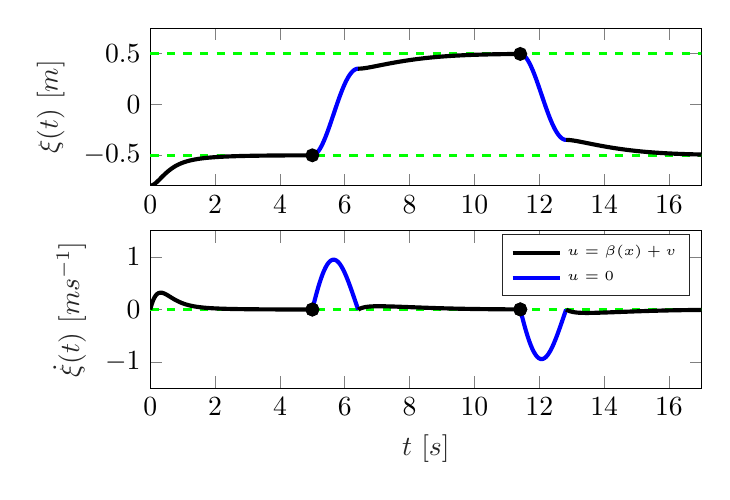
\begin{tikzpicture}

\begin{axis}[%
width=7cm,
height=2cm,
at={(0.758in,1.9in)},
scale only axis,
xmin=0,
xmax=17,
xlabel style={font=\color{white!15!black}},
xlabel={$t$ [$s$]},
ymin=-0.8,
ymax=0.75,
ylabel style={font=\color{white!15!black}},
ylabel={$\xi(t)~[m]$},
axis background/.style={fill=white},
legend style={legend cell align=left, align=left, draw=white!15!black}
]
\addplot [color=green, dashed, line width=1.0pt]
  table[row sep=crcr]{%
0	0.5\\
17.828	0.5\\
};
%\addlegendentry{data1}

\addplot [color=green, dashed, line width=1.0pt]
  table[row sep=crcr]{%
0	-0.5\\
17.828	-0.5\\
};
%\addlegendentry{data2}

\addplot [color=black, line width=1.5pt]
  table[row sep=crcr]{%
0	-0.8\\
0.00201272951242755	-0.799994961191618\\
0.00402545902485509	-0.799979912367723\\
0.00603818853728264	-0.799954954570979\\
0.00805091804971019	-0.799920188365097\\
0.0181145656118479	-0.799602716042907\\
0.0281782131739857	-0.799054842548506\\
0.0382418607361234	-0.798288597012259\\
0.0483055082982611	-0.797315700639723\\
0.0872883339796663	-0.79180232817447\\
0.126271159661072	-0.783973965721385\\
0.165253985342477	-0.774381288683226\\
0.204236811023882	-0.763501882011192\\
0.258325242573133	-0.747042020860754\\
0.312413674122383	-0.72976988716146\\
0.366502105671634	-0.712355838953056\\
0.420590537220884	-0.69531812887462\\
0.481968041514646	-0.676898302324055\\
0.543345545808408	-0.659689888119161\\
0.60472305010217	-0.643832734591055\\
0.666100554395931	-0.629420387260955\\
0.724027870722878	-0.61714861623052\\
0.781955187049825	-0.606081387447396\\
0.839882503376772	-0.596135540852008\\
0.897809819703719	-0.587228440080926\\
0.966381939079961	-0.577900541883002\\
1.0349540584562	-0.569737335894573\\
1.10352617783245	-0.562593329727953\\
1.17209829720869	-0.556334145892474\\
1.24444068335681	-0.550553176429767\\
1.31678306950493	-0.54550217235343\\
1.38912545565305	-0.541079788374854\\
1.46146784180118	-0.537189412277445\\
1.5338102279493	-0.533747712761737\\
1.60615261409742	-0.530698125658422\\
1.67849500024554	-0.527988925895292\\
1.75083738639366	-0.525569970593653\\
1.83596904357362	-0.52303674293993\\
1.92110070075358	-0.520801579050654\\
2.00623235793354	-0.518824975490308\\
2.0913640151135	-0.517065812797719\\
2.18740015096789	-0.515299213028131\\
2.28343628682228	-0.513739062989125\\
2.37947242267667	-0.512359606745628\\
2.47550855853105	-0.511132507072772\\
2.58940334197328	-0.509841944435238\\
2.7032981254155	-0.508712751315759\\
2.81719290885772	-0.507725193949768\\
2.93108769229994	-0.506855883378508\\
3.05608769229994	-0.506014933876777\\
3.18108769229994	-0.505281771732899\\
3.30608769229994	-0.504643252864409\\
3.43108769229994	-0.504084307800779\\
3.55608769229994	-0.503592377814803\\
3.68108769229994	-0.503161214961675\\
3.80608769229994	-0.502783544826694\\
3.93108769229994	-0.502451790226188\\
4.05608769229994	-0.502159488130832\\
4.18108769229994	-0.501902551685047\\
4.30608769229994	-0.501676794421557\\
4.43108769229994	-0.501478101249754\\
4.55608769229994	-0.501302911111012\\
4.68108769229994	-0.501148668049079\\
4.80608769229994	-0.501012909399428\\
4.93108769229994	-0.500893294150882\\
4.94831576922496	-0.500877951450443\\
4.96554384614997	-0.500862873825328\\
4.98277192307499	-0.500848056637506\\
5	-0.50083349533071\\
};
%\addlegendentry{data3}

\addplot [color=blue, line width=1.5pt]
  table[row sep=crcr]{%
5	-0.50083349533071\\
5.001	-0.50083138815981\\
5.002	-0.500826778512268\\
5.003	-0.500819667662055\\
5.004	-0.500810056895002\\
5.005	-0.500797947508799\\
5.006	-0.500783340812974\\
5.007	-0.500766238128885\\
5.008	-0.500746640789707\\
5.009	-0.500724550140417\\
5.01	-0.500699967537785\\
5.011	-0.500672894350357\\
5.012	-0.500643331958447\\
5.013	-0.500611281754122\\
5.014	-0.500576745141187\\
5.015	-0.500539723535175\\
5.016	-0.500500218363335\\
5.017	-0.500458231064615\\
5.018	-0.500413763089652\\
5.019	-0.500366815900759\\
5.02	-0.50031739097191\\
5.021	-0.500265489788728\\
5.022	-0.500211113848472\\
5.023	-0.500154264660022\\
5.024	-0.500094943743869\\
5.025	-0.500033152632097\\
5.026	-0.499968892868374\\
5.027	-0.499902166007936\\
5.028	-0.499832973617573\\
5.029	-0.499761317275618\\
5.03	-0.499687198571931\\
5.031	-0.499610619107885\\
5.032	-0.499531580496354\\
5.033	-0.499450084361699\\
5.034	-0.499366132339754\\
5.035	-0.499279726077809\\
5.036	-0.499190867234601\\
5.037	-0.499099557480297\\
5.038	-0.499005798496481\\
5.039	-0.49890959197614\\
5.04	-0.498810939623647\\
5.041	-0.498709843154752\\
5.042	-0.498606304296562\\
5.043	-0.498500324787532\\
5.044	-0.498391906377448\\
5.045	-0.49828105082741\\
5.046	-0.498167759909825\\
5.047	-0.498052035408383\\
5.048	-0.49793387911805\\
5.049	-0.497813292845051\\
5.05	-0.497690278406852\\
5.051	-0.497564837632153\\
5.052	-0.497436972360863\\
5.053	-0.497306684444096\\
5.054	-0.497173975744148\\
5.055	-0.497038848134484\\
5.056	-0.496901303499726\\
5.057	-0.496761343735636\\
5.058	-0.4966189707491\\
5.059	-0.496474186458115\\
5.06	-0.496326992791771\\
5.061	-0.49617739169024\\
5.062	-0.496025385104756\\
5.063	-0.495870974997602\\
5.064	-0.495714163342098\\
5.065	-0.495554952122578\\
5.066	-0.495393343334382\\
5.067	-0.495229338983836\\
5.068	-0.495062941088238\\
5.069	-0.494894151675843\\
5.07	-0.494722972785846\\
5.071	-0.494549406468367\\
5.072	-0.494373454784437\\
5.073	-0.494195119805977\\
5.074	-0.49401440361579\\
5.075	-0.493831308307538\\
5.076	-0.493645835985731\\
5.077	-0.493457988765707\\
5.078	-0.493267768773619\\
5.079	-0.49307517814642\\
5.08	-0.492880219031842\\
5.081	-0.492682893588384\\
5.082	-0.492483203985296\\
5.083	-0.492281152402559\\
5.084	-0.492076741030874\\
5.085	-0.491869972071641\\
5.086	-0.491660847736945\\
5.087	-0.491449370249538\\
5.088	-0.491235541842827\\
5.089	-0.491019364760851\\
5.09	-0.49080084125827\\
5.091	-0.490579973600343\\
5.092	-0.490356764062918\\
5.093	-0.490131214932411\\
5.094	-0.489903328505787\\
5.095	-0.489673107090551\\
5.096	-0.489440553004723\\
5.097	-0.489205668576827\\
5.098	-0.488968456145871\\
5.099	-0.48872891806133\\
5.1	-0.48848705668313\\
5.101	-0.488242874381633\\
5.102	-0.487996373537617\\
5.103	-0.487747556542257\\
5.104	-0.487496425797114\\
5.105	-0.487242983714113\\
5.106	-0.486987232715527\\
5.107	-0.48672917523396\\
5.108	-0.486468813712329\\
5.109	-0.486206150603849\\
5.11	-0.485941188372012\\
5.111	-0.485673929490572\\
5.112	-0.485404376443526\\
5.113	-0.485132531725098\\
5.114	-0.48485839783972\\
5.115	-0.484581977302018\\
5.116	-0.484303272636786\\
5.117	-0.484022286378978\\
5.118	-0.483739021073686\\
5.119	-0.483453479276118\\
5.12	-0.48316566355159\\
5.121	-0.482875576475498\\
5.122	-0.482583220633306\\
5.123	-0.482288598620527\\
5.124	-0.481991713042705\\
5.125	-0.481692566515396\\
5.126	-0.481391161664148\\
5.127	-0.481087501124491\\
5.128	-0.480781587541907\\
5.129	-0.480473423571822\\
5.13	-0.480163011879583\\
5.131	-0.479850355140439\\
5.132	-0.479535456039526\\
5.133	-0.479218317271846\\
5.134	-0.478898941542249\\
5.135	-0.478577331565415\\
5.136	-0.478253490065835\\
5.137	-0.477927419777795\\
5.138	-0.477599123445353\\
5.139	-0.477268603822325\\
5.14	-0.476935863672261\\
5.141	-0.476600905768431\\
5.142	-0.476263732893807\\
5.143	-0.475924347841039\\
5.144	-0.475582753412439\\
5.145	-0.475238952419964\\
5.146	-0.474892947685194\\
5.147	-0.474544742039317\\
5.148	-0.474194338323105\\
5.149	-0.473841739386897\\
5.15	-0.473486948090584\\
5.151	-0.473129967303583\\
5.152	-0.472770799904823\\
5.153	-0.472409448782724\\
5.154	-0.472045916835179\\
5.155	-0.471680206969531\\
5.156	-0.47131232210256\\
5.157	-0.470942265160457\\
5.158	-0.470570039078811\\
5.159	-0.470195646802585\\
5.16	-0.469819091286097\\
5.161	-0.469440375493005\\
5.162	-0.46905950239628\\
5.163	-0.468676474978194\\
5.164	-0.468291296230295\\
5.165	-0.467903969153392\\
5.166	-0.467514496757531\\
5.167	-0.467122882061978\\
5.168	-0.466729128095198\\
5.169	-0.466333237894836\\
5.17	-0.465935214507697\\
5.171	-0.465535060989727\\
5.172	-0.465132780405992\\
5.173	-0.464728375830658\\
5.174	-0.464321850346972\\
5.175	-0.463913207047241\\
5.176	-0.463502449032814\\
5.177	-0.46308957941406\\
5.178	-0.462674601310348\\
5.179	-0.462257517850029\\
5.18	-0.461838332170411\\
5.181	-0.461417047417748\\
5.182	-0.460993666747207\\
5.183	-0.460568193322861\\
5.184	-0.460140630317659\\
5.185	-0.459710980913409\\
5.186	-0.45927924830076\\
5.187	-0.458845435679179\\
5.188	-0.458409546256929\\
5.189	-0.457971583251053\\
5.19	-0.45753154988735\\
5.191	-0.457089449400357\\
5.192	-0.456645285033326\\
5.193	-0.456199060038205\\
5.194	-0.455750777675616\\
5.195	-0.455300441214836\\
5.196	-0.454848053933778\\
5.197	-0.454393619118963\\
5.198	-0.45393714006551\\
5.199	-0.453478620077105\\
5.2	-0.453018062465987\\
5.201	-0.452555470552923\\
5.202	-0.452090847667192\\
5.203	-0.451624197146558\\
5.204	-0.451155522337254\\
5.205	-0.450684826593958\\
5.206	-0.450212113279774\\
5.207	-0.449737385766211\\
5.208	-0.44926064743316\\
5.209	-0.448781901668874\\
5.21	-0.448301151869947\\
5.211	-0.447818401441293\\
5.212	-0.447333653796124\\
5.213	-0.446846912355932\\
5.214	-0.446358180550462\\
5.215	-0.445867461817695\\
5.216	-0.445374759603825\\
5.217	-0.444880077363241\\
5.218	-0.444383418558498\\
5.219	-0.443884786660306\\
5.22	-0.443384185147499\\
5.221	-0.442881617507019\\
5.222	-0.442377087233894\\
5.223	-0.441870597831214\\
5.224	-0.441362152810112\\
5.225	-0.440851755689741\\
5.226	-0.440339409997254\\
5.227	-0.439825119267781\\
5.228	-0.439308887044406\\
5.229	-0.438790716878149\\
5.23	-0.438270612327941\\
5.231	-0.437748576960605\\
5.232	-0.437224614350829\\
5.233	-0.436698728081153\\
5.234	-0.436170921741939\\
5.235	-0.435641198931352\\
5.236	-0.435109563255339\\
5.237	-0.434576018327607\\
5.238	-0.4340405677696\\
5.239	-0.433503215210478\\
5.24	-0.432963964287092\\
5.241	-0.432422818643969\\
5.242	-0.43187978193328\\
5.243	-0.431334857814829\\
5.244	-0.430788049956021\\
5.245	-0.430239362031845\\
5.246	-0.429688797724852\\
5.247	-0.429136360725132\\
5.248	-0.428582054730289\\
5.249	-0.428025883445425\\
5.25	-0.42746785058311\\
5.251	-0.426907959863368\\
5.252	-0.426346215013646\\
5.253	-0.4257826197688\\
5.254	-0.425217177871066\\
5.255	-0.424649893070042\\
5.256	-0.424080769122663\\
5.257	-0.423509809793179\\
5.258	-0.422937018853133\\
5.259	-0.422362400081341\\
5.26	-0.421785957263863\\
5.261	-0.421207694193988\\
5.262	-0.420627614672205\\
5.263	-0.420045722506185\\
5.264	-0.419462021510755\\
5.265	-0.418876515507879\\
5.266	-0.418289208326631\\
5.267	-0.417700103803177\\
5.268	-0.417109205780748\\
5.269	-0.41651651810962\\
5.27	-0.415922044647089\\
5.271	-0.415325789257452\\
5.272	-0.414727755811979\\
5.273	-0.414127948188896\\
5.274	-0.413526370273356\\
5.275	-0.412923025957421\\
5.276	-0.412317919140037\\
5.277	-0.41171105372701\\
5.278	-0.411102433630985\\
5.279	-0.410492062771425\\
5.28	-0.409879945074581\\
5.281	-0.409266084473477\\
5.282	-0.408650484907881\\
5.283	-0.408033150324285\\
5.284	-0.407414084675882\\
5.285	-0.40679329192254\\
5.286	-0.406170776030784\\
5.287	-0.405546540973766\\
5.288	-0.404920590731249\\
5.289	-0.404292929289579\\
5.29	-0.403663560641663\\
5.291	-0.403032488786945\\
5.292	-0.402399717731387\\
5.293	-0.401765251487438\\
5.294	-0.401129094074018\\
5.295	-0.400491249516491\\
5.296	-0.399851721846643\\
5.297	-0.399210515102658\\
5.298	-0.398567633329092\\
5.299	-0.397923080576857\\
5.3	-0.397276860903189\\
5.301	-0.39662897837163\\
5.302	-0.395979437052004\\
5.303	-0.395328241020388\\
5.304	-0.394675394359099\\
5.305	-0.394020901156661\\
5.306	-0.393364765507785\\
5.307	-0.392706991513346\\
5.308	-0.392047583280358\\
5.309	-0.391386544921953\\
5.31	-0.390723880557353\\
5.311	-0.39005959431185\\
5.312	-0.389393690316782\\
5.313	-0.388726172709509\\
5.314	-0.388057045633385\\
5.315	-0.387386313237744\\
5.316	-0.386713979677866\\
5.317	-0.386040049114958\\
5.318	-0.385364525716134\\
5.319	-0.384687413654381\\
5.32	-0.384008717108547\\
5.321	-0.383328440263308\\
5.322	-0.382646587309149\\
5.323	-0.381963162442338\\
5.324	-0.381278169864905\\
5.325	-0.380591613784614\\
5.326	-0.379903498414941\\
5.327	-0.379213827975053\\
5.328	-0.378522606689779\\
5.329	-0.377829838789588\\
5.33	-0.377135528510568\\
5.331	-0.376439680094396\\
5.332	-0.375742297788321\\
5.333	-0.375043385845134\\
5.334	-0.374342948523147\\
5.335	-0.373640990086169\\
5.336	-0.37293751480348\\
5.337	-0.37223252694981\\
5.338	-0.371526030805311\\
5.339	-0.370818030655537\\
5.34	-0.370108530791418\\
5.341	-0.369397535509233\\
5.342	-0.368685049110591\\
5.343	-0.367971075902405\\
5.344	-0.367255620196865\\
5.345	-0.366538686311418\\
5.346	-0.36582027856874\\
5.347	-0.365100401296717\\
5.348	-0.364379058828412\\
5.349	-0.363656255502052\\
5.35	-0.362931995660995\\
5.351	-0.362206283653707\\
5.352	-0.361479123833743\\
5.353	-0.360750520559716\\
5.354	-0.360020478195278\\
5.355	-0.359289001109091\\
5.356	-0.358556093674807\\
5.357	-0.357821760271041\\
5.358	-0.357086005281347\\
5.359	-0.356348833094194\\
5.36	-0.355610248102942\\
5.361	-0.354870254705817\\
5.362	-0.354128857305887\\
5.363	-0.353386060311035\\
5.364	-0.35264186813394\\
5.365	-0.351896285192048\\
5.366	-0.351149315907548\\
5.367	-0.350400964707351\\
5.368	-0.349651236023059\\
5.369	-0.348900134290949\\
5.37	-0.348147663951941\\
5.371	-0.347393829451576\\
5.372	-0.346638635239994\\
5.373	-0.345882085771906\\
5.374	-0.345124185506572\\
5.375	-0.344364938907772\\
5.376	-0.34360435044379\\
5.377	-0.342842424587379\\
5.378	-0.342079165815744\\
5.379	-0.341314578610515\\
5.38	-0.340548667457721\\
5.381	-0.339781436847767\\
5.382	-0.33901289127541\\
5.383	-0.338243035239732\\
5.384	-0.337471873244117\\
5.385	-0.336699409796227\\
5.386	-0.335925649407976\\
5.387	-0.335150596595505\\
5.388	-0.334374255879158\\
5.389	-0.333596631783458\\
5.39	-0.332817728837081\\
5.391	-0.332037551572833\\
5.392	-0.331256104527622\\
5.393	-0.330473392242438\\
5.394	-0.329689419262324\\
5.395	-0.328904190136352\\
5.396	-0.328117709417603\\
5.397	-0.327329981663135\\
5.398	-0.326541011433961\\
5.399	-0.325750803295029\\
5.4	-0.32495936181519\\
5.401	-0.324166691567175\\
5.402	-0.323372797127576\\
5.403	-0.322577683076813\\
5.404	-0.321781353999114\\
5.405	-0.320983814482489\\
5.406	-0.320185069118705\\
5.407	-0.319385122503263\\
5.408	-0.31858397923537\\
5.409	-0.317781643917915\\
5.41	-0.316978121157447\\
5.411	-0.316173415564147\\
5.412	-0.315367531751803\\
5.413	-0.314560474337789\\
5.414	-0.313752247943034\\
5.415	-0.312942857192005\\
5.416	-0.312132306712673\\
5.417	-0.311320601136496\\
5.418	-0.310507745098389\\
5.419	-0.309693743236703\\
5.42	-0.308878600193196\\
5.421	-0.308062320613011\\
5.422	-0.30724490914465\\
5.423	-0.30642637043995\\
5.424	-0.305606709154058\\
5.425	-0.304785929945403\\
5.426	-0.303964037475677\\
5.427	-0.303141036409803\\
5.428	-0.302316931415917\\
5.429	-0.301491727165337\\
5.43	-0.300665428332544\\
5.431	-0.29983803959515\\
5.432	-0.299009565633881\\
5.433	-0.298180011132544\\
5.434	-0.297349380778009\\
5.435	-0.296517679260181\\
5.436	-0.295684911271972\\
5.437	-0.294851081509283\\
5.438	-0.294016194670973\\
5.439	-0.293180255458837\\
5.44	-0.292343268577579\\
5.441	-0.29150523873479\\
5.442	-0.290666170640921\\
5.443	-0.289826069009256\\
5.444	-0.288984938555894\\
5.445	-0.288142783999714\\
5.446	-0.287299610062359\\
5.447	-0.286455421468207\\
5.448	-0.285610222944344\\
5.449	-0.284764019220545\\
5.45	-0.283916815029243\\
5.451	-0.283068615105506\\
5.452	-0.282219424187015\\
5.453	-0.281369247014034\\
5.454	-0.280518088329389\\
5.455	-0.279665952878441\\
5.456	-0.278812845409061\\
5.457	-0.277958770671608\\
5.458	-0.277103733418898\\
5.459	-0.276247738406184\\
5.46	-0.27539079039113\\
5.461	-0.274532894133786\\
5.462	-0.273674054396562\\
5.463	-0.272814275944203\\
5.464	-0.271953563543765\\
5.465	-0.27109192196459\\
5.466	-0.270229355978281\\
5.467	-0.269365870358675\\
5.468	-0.268501469881822\\
5.469	-0.267636159325956\\
5.47	-0.266769943471473\\
5.471	-0.265902827100903\\
5.472	-0.265034814998888\\
5.473	-0.264165911952157\\
5.474	-0.263296122749496\\
5.475	-0.262425452181731\\
5.476	-0.261553905041698\\
5.477	-0.260681486124216\\
5.478	-0.259808200226069\\
5.479	-0.258934052145975\\
5.48	-0.258059046684562\\
5.481	-0.257183188644348\\
5.482	-0.256306482829707\\
5.483	-0.255428934046852\\
5.484	-0.254550547103809\\
5.485	-0.253671326810387\\
5.486	-0.252791277978158\\
5.487	-0.25191040542043\\
5.488	-0.251028713952223\\
5.489	-0.250146208390245\\
5.49	-0.249262893552862\\
5.491	-0.24837877426008\\
5.492	-0.247493855333516\\
5.493	-0.246608141596373\\
5.494	-0.245721637873417\\
5.495	-0.244834348990952\\
5.496	-0.243946279776792\\
5.497	-0.24305743506024\\
5.498	-0.242167819672062\\
5.499	-0.24127743844446\\
5.5	-0.240386296211049\\
5.501	-0.239494397806833\\
5.502	-0.238601748068179\\
5.503	-0.23770835183279\\
5.504	-0.236814213939685\\
5.505	-0.23591933922917\\
5.506	-0.235023732542814\\
5.507	-0.234127398723427\\
5.508	-0.233230342615032\\
5.509	-0.232332569062839\\
5.51	-0.231434082913225\\
5.511	-0.230534889013706\\
5.512	-0.229634992212912\\
5.513	-0.228734397360563\\
5.514	-0.227833109307444\\
5.515	-0.226931132905382\\
5.516	-0.226028473007217\\
5.517	-0.225125134466782\\
5.518	-0.224221122138875\\
5.519	-0.223316440879235\\
5.52	-0.222411095544518\\
5.521	-0.221505090992272\\
5.522	-0.220598432080913\\
5.523	-0.219691123669696\\
5.524	-0.218783170618698\\
5.525	-0.217874577788787\\
5.526	-0.216965350041597\\
5.527	-0.21605549223951\\
5.528	-0.215145009245624\\
5.529	-0.214233905923732\\
5.53	-0.213322187138296\\
5.531	-0.212409857754424\\
5.532	-0.211496922637844\\
5.533	-0.210583386654878\\
5.534	-0.209669254672422\\
5.535	-0.208754531557915\\
5.536	-0.207839222179321\\
5.537	-0.2069233314051\\
5.538	-0.206006864104183\\
5.539	-0.205089825145952\\
5.54	-0.20417221940021\\
5.541	-0.20325405173716\\
5.542	-0.20233532702738\\
5.543	-0.201416050141797\\
5.544	-0.200496225951662\\
5.545	-0.199575859328531\\
5.546	-0.198654955144232\\
5.547	-0.197733518270846\\
5.548	-0.196811553580683\\
5.549	-0.195889065946254\\
5.55	-0.194966060240249\\
5.551	-0.194042541335512\\
5.552	-0.193118514105018\\
5.553	-0.192193983421844\\
5.554	-0.191268954159151\\
5.555	-0.190343431190153\\
5.556	-0.189417419388099\\
5.557	-0.188490923626243\\
5.558	-0.187563948777825\\
5.559	-0.186636499716041\\
5.56	-0.185708581314023\\
5.561	-0.184780198444813\\
5.562	-0.183851355981338\\
5.563	-0.182922058796388\\
5.564	-0.181992311762589\\
5.565	-0.181062119752381\\
5.566	-0.180131487637991\\
5.567	-0.179200420291413\\
5.568	-0.178268922584379\\
5.569	-0.177336999388339\\
5.57	-0.176404655574431\\
5.571	-0.175471896013466\\
5.572	-0.174538725575895\\
5.573	-0.173605149131788\\
5.574	-0.172671171550812\\
5.575	-0.171736797702204\\
5.576	-0.170802032454747\\
5.577	-0.169866880676748\\
5.578	-0.168931347236012\\
5.579	-0.167995436999819\\
5.58	-0.167059154834899\\
5.581	-0.166122505607409\\
5.582	-0.165185494182907\\
5.583	-0.164248125426331\\
5.584	-0.163310404201973\\
5.585	-0.162372335373455\\
5.586	-0.161433923803704\\
5.587	-0.160495174354933\\
5.588	-0.15955609188861\\
5.589	-0.158616681265439\\
5.59	-0.157676947345334\\
5.591	-0.156736894987398\\
5.592	-0.155796529049894\\
5.593	-0.154855854390224\\
5.594	-0.153914875864908\\
5.595	-0.152973598329555\\
5.596	-0.152032026638841\\
5.597	-0.151090165646488\\
5.598	-0.150148020205235\\
5.599	-0.14920559516682\\
5.6	-0.148262895381952\\
5.601	-0.147319925700288\\
5.602	-0.146376690970411\\
5.603	-0.145433196039804\\
5.604	-0.144489445754829\\
5.605	-0.143545444960702\\
5.606	-0.142601198501467\\
5.607	-0.141656711219977\\
5.608	-0.140711987957867\\
5.609	-0.139767033555531\\
5.61	-0.1388218528521\\
5.611	-0.137876450685416\\
5.612	-0.13693083189201\\
5.613	-0.135985001307079\\
5.614	-0.135038963764461\\
5.615	-0.134092724096612\\
5.616	-0.133146287134584\\
5.617	-0.132199657707998\\
5.618	-0.131252840645026\\
5.619	-0.130305840772362\\
5.62	-0.129358662915201\\
5.621	-0.128411311897218\\
5.622	-0.12746379254054\\
5.623	-0.126516109665726\\
5.624	-0.125568268091743\\
5.625	-0.124620272635942\\
5.626	-0.123672128114034\\
5.627	-0.122723839340071\\
5.628	-0.121775411126417\\
5.629	-0.120826848283727\\
5.63	-0.119878155620927\\
5.631	-0.118929337945185\\
5.632	-0.117980400061894\\
5.633	-0.117031346774644\\
5.634	-0.1160821828852\\
5.635	-0.115132913193481\\
5.636	-0.114183542497535\\
5.637	-0.113234075593516\\
5.638	-0.112284517275662\\
5.639	-0.111334872336272\\
5.64	-0.110385145565682\\
5.641	-0.109435341752242\\
5.642	-0.108485465682292\\
5.643	-0.107535522140145\\
5.644	-0.106585515908056\\
5.645	-0.105635451766205\\
5.646	-0.104685334492669\\
5.647	-0.103735168863406\\
5.648	-0.102784959652226\\
5.649	-0.101834711630771\\
5.65	-0.100884429568491\\
5.651	-0.0999341182326237\\
5.652	-0.098983782388169\\
5.653	-0.0980334267978677\\
5.654	-0.0970830562221785\\
5.655	-0.0961326754192551\\
5.656	-0.0951822891449244\\
5.657	-0.0942319021526632\\
5.658	-0.0932815191935751\\
5.659	-0.0923311450163692\\
5.66	-0.0913807843673368\\
5.661	-0.0904304419903294\\
5.662	-0.0894801226267348\\
5.663	-0.0885298310154567\\
5.664	-0.0875795718928907\\
5.665	-0.0866293499929027\\
5.666	-0.0856791700468059\\
5.667	-0.0847290367833387\\
5.668	-0.0837789549286425\\
5.669	-0.0828289292062394\\
5.67	-0.0818789643370093\\
5.671	-0.0809290650391687\\
5.672	-0.0799792360282472\\
5.673	-0.0790294820170659\\
5.674	-0.078079807715716\\
5.675	-0.0771302178315346\\
5.676	-0.0761807170690847\\
5.677	-0.0752313101301312\\
5.678	-0.074282001713621\\
5.679	-0.0733327965156584\\
5.68	-0.0723836992294845\\
5.681	-0.0714347145454556\\
5.682	-0.0704858471510201\\
5.683	-0.0695371017306966\\
5.684	-0.068588482966053\\
5.685	-0.0676399955356836\\
5.686	-0.0666916441151873\\
5.687	-0.0657434333771459\\
5.688	-0.0647953679911028\\
5.689	-0.0638474526235399\\
5.69	-0.0628996919378569\\
5.691	-0.0619520905943494\\
5.692	-0.0610046532501862\\
5.693	-0.0600573845593895\\
5.694	-0.0591102891728104\\
5.695	-0.0581633717381106\\
5.696	-0.0572166368997377\\
5.697	-0.0562700892989052\\
5.698	-0.0553237335735711\\
5.699	-0.0543775743584153\\
5.7	-0.0534316162848192\\
5.701	-0.0524858639808429\\
5.702	-0.0515403220712049\\
5.703	-0.0505949951772607\\
5.704	-0.04964988791698\\
5.705	-0.0487050049049264\\
5.706	-0.0477603507522364\\
5.707	-0.0468159300665964\\
5.708	-0.045871747452224\\
5.709	-0.044927807509844\\
5.71	-0.0439841148366686\\
5.711	-0.0430406740263765\\
5.712	-0.0420974896690902\\
5.713	-0.0411545663513569\\
5.714	-0.0402119086561252\\
5.715	-0.0392695211627254\\
5.716	-0.0383274084468481\\
5.717	-0.0373855750805235\\
5.718	-0.0364440256320989\\
5.719	-0.0355027646662197\\
5.72	-0.034561796743807\\
5.721	-0.0336211264220374\\
5.722	-0.0326807582543221\\
5.723	-0.031740696790285\\
5.724	-0.0308009465757431\\
5.725	-0.0298615121526855\\
5.726	-0.0289223980592517\\
5.727	-0.0279836088297118\\
5.728	-0.0270451489944456\\
5.729	-0.026107023079921\\
5.73	-0.025169235608675\\
5.731	-0.0242317910992912\\
5.732	-0.023294694066381\\
5.733	-0.022357949020561\\
5.734	-0.0214215604684348\\
5.735	-0.0204855329125704\\
5.736	-0.0195498708514806\\
5.737	-0.0186145787796028\\
5.738	-0.0176796611872781\\
5.739	-0.0167451225607312\\
5.74	-0.0158109673820496\\
5.741	-0.014877200129164\\
5.742	-0.0139438252758269\\
5.743	-0.0130108472915937\\
5.744	-0.0120782706418014\\
5.745	-0.0111460997875486\\
5.746	-0.0102143391856755\\
5.747	-0.00928299328874372\\
5.748	-0.00835206654501644\\
5.749	-0.00742156339843743\\
5.75	-0.00649148828861231\\
5.751	-0.00556184565078693\\
5.752	-0.00463263991582918\\
5.753	-0.00370387551020739\\
5.754	-0.00277555685597122\\
5.755	-0.00184768837073223\\
5.756	-0.000920274467642927\\
5.757	6.68044462262888e-06\\
5.758	0.000933171961888126\\
5.759	0.00185919568449575\\
5.76	0.00278474721732472\\
5.761	0.00370982216981178\\
5.762	0.00463441615597144\\
5.763	0.0055585247944138\\
5.764	0.00648214370836574\\
5.765	0.00740526852569016\\
5.766	0.00832789487890546\\
5.767	0.00925001840520382\\
5.768	0.0101716347464734\\
5.769	0.0110927395493152\\
5.77	0.0120133284650631\\
5.771	0.0129333971498045\\
5.772	0.0138529412643983\\
5.773	0.0147719564744945\\
5.774	0.0156904384505535\\
5.775	0.016608382867866\\
5.776	0.0175257854065708\\
5.777	0.0184426417516757\\
5.778	0.0193589475930751\\
5.779	0.0202746986255699\\
5.78	0.0211898905488866\\
5.781	0.0221045190676959\\
5.782	0.0230185798916319\\
5.783	0.0239320687353115\\
5.784	0.0248449813183527\\
5.785	0.0257573133653935\\
5.786	0.0266690606061114\\
5.787	0.0275802187752418\\
5.788	0.0284907836125964\\
5.789	0.0294007508630828\\
5.79	0.0303101162767225\\
5.791	0.0312188756086704\\
5.792	0.0321270246192321\\
5.793	0.0330345590738844\\
5.794	0.0339414747432919\\
5.795	0.034847767403327\\
5.796	0.0357534328350879\\
5.797	0.0366584668249169\\
5.798	0.0375628651644191\\
5.799	0.0384666236504805\\
5.8	0.0393697380852871\\
5.801	0.0402722042763421\\
5.802	0.0411740180364855\\
5.803	0.0420751751839116\\
5.804	0.0429756715421865\\
5.805	0.0438755029402681\\
5.806	0.0447746652125227\\
5.807	0.0456731541987439\\
5.808	0.0465709657441705\\
5.809	0.0474680956995043\\
5.81	0.0483645399209289\\
5.811	0.0492602942701261\\
5.812	0.0501553546142957\\
5.813	0.0510497168261723\\
5.814	0.0519433767840434\\
5.815	0.0528363303717672\\
5.816	0.0537285734787899\\
5.817	0.0546201020001652\\
5.818	0.0555109118365698\\
5.819	0.0564009988943225\\
5.82	0.0572903590854011\\
5.821	0.0581789883274605\\
5.822	0.0590668825438503\\
5.823	0.0599540376636316\\
5.824	0.0608404496215958\\
5.825	0.0617261143582802\\
5.826	0.0626110278199877\\
5.827	0.063495185958802\\
5.828	0.0643785847326066\\
5.829	0.065261220105101\\
5.83	0.0661430880458184\\
5.831	0.0670241845301432\\
5.832	0.0679045055393278\\
5.833	0.0687840470605097\\
5.834	0.0696628050867292\\
5.835	0.0705407756169459\\
5.836	0.0714179546560553\\
5.837	0.0722943382149071\\
5.838	0.073169922310322\\
5.839	0.0740447029651068\\
5.84	0.0749186762080734\\
5.841	0.0757918380740547\\
5.842	0.0766641846039215\\
5.843	0.0775357118445994\\
5.844	0.0784064158490856\\
5.845	0.0792762926764652\\
5.846	0.0801453383919281\\
5.847	0.081013549066786\\
5.848	0.0818809207784881\\
5.849	0.0827474496106383\\
5.85	0.083613131653012\\
5.851	0.0844779630015715\\
5.852	0.0853419397584835\\
5.853	0.0862050580321349\\
5.854	0.0870673139371488\\
5.855	0.0879287035944021\\
5.856	0.0887892231310399\\
5.857	0.0896488686804942\\
5.858	0.0905076363824969\\
5.859	0.091365522383099\\
5.86	0.0922225228346851\\
5.861	0.0930786338959894\\
5.862	0.0939338517321123\\
5.863	0.0947881725145364\\
5.864	0.0956415924211421\\
5.865	0.0964941076362229\\
5.866	0.0973457143505036\\
5.867	0.0981964087611527\\
5.868	0.0990461870718016\\
5.869	0.0998950454925577\\
5.87	0.100742980240022\\
5.871	0.101589987537303\\
5.872	0.102436063614033\\
5.873	0.103281204706386\\
5.874	0.10412540705709\\
5.875	0.104968666915443\\
5.876	0.105810980537329\\
5.877	0.106652344185236\\
5.878	0.107492754128266\\
5.879	0.108332206642155\\
5.88	0.109170698009286\\
5.881	0.110008224518705\\
5.882	0.110844782466137\\
5.883	0.111680368153999\\
5.884	0.112514977891418\\
5.885	0.113348607994241\\
5.886	0.114181254785057\\
5.887	0.115012914593209\\
5.888	0.115843583754805\\
5.889	0.116673258612739\\
5.89	0.117501935516704\\
5.891	0.118329610823205\\
5.892	0.119156280895574\\
5.893	0.119981942103987\\
5.894	0.120806590825479\\
5.895	0.121630223443954\\
5.896	0.122452836350206\\
5.897	0.123274425941928\\
5.898	0.12409498862373\\
5.899	0.124914520807152\\
5.9	0.125733018910681\\
5.901	0.12655047935976\\
5.902	0.127366898586809\\
5.903	0.128182273031234\\
5.904	0.128996599139445\\
5.905	0.129809873364867\\
5.906	0.130622092167958\\
5.907	0.131433252016219\\
5.908	0.132243349384212\\
5.909	0.133052380753572\\
5.91	0.13386034261302\\
5.911	0.13466723145838\\
5.912	0.135473043792591\\
5.913	0.136277776125721\\
5.914	0.137081424974981\\
5.915	0.137883986864739\\
5.916	0.138685458326536\\
5.917	0.139485835899093\\
5.918	0.140285116128335\\
5.919	0.141083295567394\\
5.92	0.14188037077663\\
5.921	0.142676338323641\\
5.922	0.14347119478328\\
5.923	0.144264936737663\\
5.924	0.145057560776189\\
5.925	0.145849063495546\\
5.926	0.146639441499733\\
5.927	0.147428691400064\\
5.928	0.148216809815191\\
5.929	0.149003793371109\\
5.93	0.149789638701172\\
5.931	0.150574342446108\\
5.932	0.151357901254032\\
5.933	0.152140311780455\\
5.934	0.152921570688302\\
5.935	0.153701674647921\\
5.936	0.154480620337099\\
5.937	0.155258404441073\\
5.938	0.156035023652543\\
5.939	0.156810474671687\\
5.94	0.157584754206171\\
5.941	0.158357858971161\\
5.942	0.15912978568934\\
5.943	0.159900531090917\\
5.944	0.16067009191364\\
5.945	0.16143846490281\\
5.946	0.162205646811292\\
5.947	0.162971634399529\\
5.948	0.163736424435553\\
5.949	0.164500013694996\\
5.95	0.165262398961107\\
5.951	0.166023577024761\\
5.952	0.166783544684469\\
5.953	0.167542298746397\\
5.954	0.16829983602437\\
5.955	0.169056153339891\\
5.956	0.169811247522148\\
5.957	0.17056511540803\\
5.958	0.171317753842136\\
5.959	0.172069159676788\\
5.96	0.172819329772043\\
5.961	0.173568260995706\\
5.962	0.174315950223339\\
5.963	0.175062394338273\\
5.964	0.175807590231625\\
5.965	0.176551534802302\\
5.966	0.177294224957017\\
5.967	0.178035657610302\\
5.968	0.178775829684513\\
5.969	0.17951473810985\\
5.97	0.180252379824361\\
5.971	0.18098875177396\\
5.972	0.181723850912432\\
5.973	0.182457674201447\\
5.974	0.183190218610573\\
5.975	0.183921481117286\\
5.976	0.184651458706978\\
5.977	0.185380148372975\\
5.978	0.186107547116541\\
5.979	0.186833651946892\\
5.98	0.187558459881209\\
5.981	0.188281967944645\\
5.982	0.189004173170338\\
5.983	0.189725072599423\\
5.984	0.190444663281039\\
5.985	0.191162942272345\\
5.986	0.191879906638525\\
5.987	0.192595553452805\\
5.988	0.193309879796457\\
5.989	0.194022882758813\\
5.99	0.194734559437277\\
5.991	0.195444906937333\\
5.992	0.196153922372556\\
5.993	0.196861602864621\\
5.994	0.197567945543317\\
5.995	0.198272947546554\\
5.996	0.198976606020376\\
5.997	0.199678918118967\\
5.998	0.200379881004665\\
5.999	0.201079491847972\\
6	0.20177774782756\\
6.001	0.202474646130288\\
6.002	0.203170183951204\\
6.003	0.203864358493562\\
6.004	0.204557166968826\\
6.005	0.205248606596683\\
6.006	0.205938674605055\\
6.007	0.206627368230103\\
6.008	0.207314684716242\\
6.009	0.208000621316146\\
6.01	0.208685175290762\\
6.011	0.209368343909317\\
6.012	0.210050124449328\\
6.013	0.210730514196611\\
6.014	0.211409510445292\\
6.015	0.212087110497816\\
6.016	0.212763311664952\\
6.017	0.213438111265811\\
6.018	0.214111506627847\\
6.019	0.21478349508687\\
6.02	0.215454073987054\\
6.021	0.216123240680949\\
6.022	0.216790992529484\\
6.023	0.217457326901982\\
6.024	0.218122241176167\\
6.025	0.218785732738171\\
6.026	0.219447798982545\\
6.027	0.220108437312267\\
6.028	0.220767645138752\\
6.029	0.22142541988186\\
6.03	0.222081758969901\\
6.031	0.22273665983965\\
6.032	0.223390119936353\\
6.033	0.224042136713732\\
6.034	0.224692707634001\\
6.035	0.225341830167867\\
6.036	0.225989501794541\\
6.037	0.226635720001748\\
6.038	0.227280482285736\\
6.039	0.227923786151278\\
6.04	0.228565629111689\\
6.041	0.229206008688826\\
6.042	0.229844922413102\\
6.043	0.230482367823493\\
6.044	0.231118342467541\\
6.045	0.231752843901369\\
6.046	0.232385869689687\\
6.047	0.233017417405794\\
6.048	0.233647484631595\\
6.049	0.234276068957603\\
6.05	0.234903167982947\\
6.051	0.235528779315383\\
6.052	0.236152900571296\\
6.053	0.236775529375714\\
6.054	0.237396663362313\\
6.055	0.238016300173421\\
6.056	0.23863443746003\\
6.057	0.239251072881804\\
6.058	0.239866204107081\\
6.059	0.240479828812886\\
6.06	0.241091944684935\\
6.061	0.241702549417643\\
6.062	0.242311640714132\\
6.063	0.242919216286237\\
6.064	0.243525273854512\\
6.065	0.244129811148242\\
6.066	0.244732825905444\\
6.067	0.245334315872876\\
6.068	0.245934278806048\\
6.069	0.24653271246922\\
6.07	0.247129614635418\\
6.071	0.247724983086435\\
6.072	0.248318815612841\\
6.073	0.248911110013986\\
6.074	0.24950186409801\\
6.075	0.250091075681849\\
6.076	0.250678742591239\\
6.077	0.251264862660727\\
6.078	0.251849433733671\\
6.079	0.252432453662252\\
6.08	0.253013920307481\\
6.081	0.253593831539198\\
6.082	0.254172185236086\\
6.083	0.254748979285673\\
6.084	0.25532421158434\\
6.085	0.255897880037326\\
6.086	0.256469982558734\\
6.087	0.257040517071537\\
6.088	0.257609481507586\\
6.089	0.258176873807613\\
6.09	0.258742691921238\\
6.091	0.259306933806976\\
6.092	0.259869597432239\\
6.093	0.260430680773349\\
6.094	0.260990181815534\\
6.095	0.261548098552942\\
6.096	0.262104428988642\\
6.097	0.262659171134631\\
6.098	0.263212323011838\\
6.099	0.263763882650133\\
6.1	0.264313848088329\\
6.101	0.264862217374186\\
6.102	0.265408988564424\\
6.103	0.265954159724717\\
6.104	0.266497728929707\\
6.105	0.267039694263007\\
6.106	0.267580053817203\\
6.107	0.268118805693864\\
6.108	0.268655948003542\\
6.109	0.269191478865779\\
6.11	0.269725396409116\\
6.111	0.27025769877109\\
6.112	0.270788384098244\\
6.113	0.271317450546132\\
6.114	0.271844896279321\\
6.115	0.272370719471398\\
6.116	0.272894918304972\\
6.117	0.273417490971681\\
6.118	0.273938435672198\\
6.119	0.27445775061623\\
6.12	0.274975434022527\\
6.121	0.275491484118885\\
6.122	0.276005899142151\\
6.123	0.276518677338225\\
6.124	0.277029816962067\\
6.125	0.277539316277701\\
6.126	0.278047173558218\\
6.127	0.278553387085778\\
6.128	0.279057955151619\\
6.129	0.279560876056057\\
6.13	0.280062148108492\\
6.131	0.280561769627412\\
6.132	0.281059738940395\\
6.133	0.281556054384114\\
6.134	0.282050714304341\\
6.135	0.28254371705595\\
6.136	0.283035061002923\\
6.137	0.28352474451835\\
6.138	0.284012765984434\\
6.139	0.284499123792496\\
6.14	0.284983816342976\\
6.141	0.28546684204544\\
6.142	0.28594819931858\\
6.143	0.286427886590217\\
6.144	0.286905902297308\\
6.145	0.287382244885946\\
6.146	0.287856912811365\\
6.147	0.288329904537941\\
6.148	0.288801218539199\\
6.149	0.28927085329781\\
6.15	0.289738807305601\\
6.151	0.290205079063553\\
6.152	0.290669667081805\\
6.153	0.291132569879658\\
6.154	0.291593785985578\\
6.155	0.292053313937196\\
6.156	0.292511152281314\\
6.157	0.292967299573906\\
6.158	0.293421754380121\\
6.159	0.293874515274285\\
6.16	0.294325580839906\\
6.161	0.294774949669673\\
6.162	0.295222620365458\\
6.163	0.295668591538326\\
6.164	0.296112861808527\\
6.165	0.296555429805504\\
6.166	0.296996294167895\\
6.167	0.297435453543535\\
6.168	0.297872906589458\\
6.169	0.298308651971897\\
6.17	0.298742688366288\\
6.171	0.299175014457275\\
6.172	0.299605628938705\\
6.173	0.300034530513636\\
6.174	0.300461717894336\\
6.175	0.300887189802287\\
6.176	0.301310944968182\\
6.177	0.301732982131934\\
6.178	0.302153300042671\\
6.179	0.302571897458741\\
6.18	0.302988773147714\\
6.181	0.303403925886382\\
6.182	0.30381735446076\\
6.183	0.30422905766609\\
6.184	0.304639034306839\\
6.185	0.305047283196705\\
6.186	0.305453803158613\\
6.187	0.305858593024722\\
6.188	0.306261651636419\\
6.189	0.306662977844327\\
6.19	0.307062570508302\\
6.191	0.307460428497438\\
6.192	0.307856550690063\\
6.193	0.308250935973742\\
6.194	0.308643583245281\\
6.195	0.309034491410724\\
6.196	0.309423659385356\\
6.197	0.3098110860937\\
6.198	0.310196770469524\\
6.199	0.310580711455838\\
6.2	0.310962908004895\\
6.201	0.31134335907819\\
6.202	0.311722063646464\\
6.203	0.312099020689704\\
6.204	0.312474229197138\\
6.205	0.312847688167245\\
6.206	0.313219396607746\\
6.207	0.313589353535611\\
6.208	0.313957557977056\\
6.209	0.314324008967544\\
6.21	0.314688705551785\\
6.211	0.315051646783736\\
6.212	0.315412831726602\\
6.213	0.315772259452836\\
6.214	0.316129929044138\\
6.215	0.316485839591455\\
6.216	0.316839990194983\\
6.217	0.317192379964164\\
6.218	0.317543008017686\\
6.219	0.317891873483487\\
6.22	0.318238975498749\\
6.221	0.318584313209901\\
6.222	0.31892788577262\\
6.223	0.319269692351826\\
6.224	0.319609732121684\\
6.225	0.319948004265606\\
6.226	0.320284507976247\\
6.227	0.320619242455504\\
6.228	0.320952206914519\\
6.229	0.321283400573676\\
6.23	0.321612822662599\\
6.231	0.321940472420154\\
6.232	0.322266349094447\\
6.233	0.322590451942822\\
6.234	0.322912780231862\\
6.235	0.323233333237386\\
6.236	0.323552110244452\\
6.237	0.32386911054735\\
6.238	0.324184333449606\\
6.239	0.324497778263978\\
6.24	0.324809444312456\\
6.241	0.325119330926261\\
6.242	0.325427437445842\\
6.243	0.325733763220877\\
6.244	0.326038307610271\\
6.245	0.326341069982153\\
6.246	0.326642049713876\\
6.247	0.326941246192016\\
6.248	0.327238658812368\\
6.249	0.327534286979948\\
6.25	0.327828130108989\\
6.251	0.328120187622938\\
6.252	0.328410458954459\\
6.253	0.328698943545426\\
6.254	0.328985640846924\\
6.255	0.329270550319247\\
6.256	0.329553671431896\\
6.257	0.329835003663575\\
6.258	0.330114546502192\\
6.259	0.330392299444857\\
6.26	0.330668261997876\\
6.261	0.330942433676754\\
6.262	0.331214814006188\\
6.263	0.331485402520068\\
6.264	0.331754198761475\\
6.265	0.332021202282675\\
6.266	0.332286412645123\\
6.267	0.332549829419453\\
6.268	0.332811452185481\\
6.269	0.3330712805322\\
6.27	0.33332931405778\\
6.271	0.333585552369562\\
6.272	0.333839995084058\\
6.273	0.334092641826948\\
6.274	0.334343492233074\\
6.275	0.334592545946443\\
6.276	0.334839802620221\\
6.277	0.335085261916727\\
6.278	0.335328923507438\\
6.279	0.335570787072978\\
6.28	0.335810852303121\\
6.281	0.336049118896783\\
6.282	0.336285586562024\\
6.283	0.336520255016039\\
6.284	0.336753123985163\\
6.285	0.336984193204859\\
6.286	0.33721346241972\\
6.287	0.337440931383463\\
6.288	0.337666599858931\\
6.289	0.337890467618081\\
6.29	0.33811253444199\\
6.291	0.338332800120842\\
6.292	0.338551264453933\\
6.293	0.338767927249663\\
6.294	0.338982788325531\\
6.295	0.339195847508137\\
6.296	0.339407104633173\\
6.297	0.339616559545421\\
6.298	0.33982421209875\\
6.299	0.340030062156111\\
6.3	0.340234109589535\\
6.301	0.340436354280126\\
6.302	0.340636796118061\\
6.303	0.340835435002581\\
6.304	0.341032270841993\\
6.305	0.341227303553661\\
6.306	0.341420533064005\\
6.307	0.341611959308493\\
6.308	0.341801582231642\\
6.309	0.34198940178701\\
6.31	0.342175417937193\\
6.311	0.342359630653819\\
6.312	0.342542039917548\\
6.313	0.342722645718063\\
6.314	0.342901448054067\\
6.315	0.343078446933278\\
6.316	0.343253642372428\\
6.317	0.343427034397252\\
6.318	0.34359862304249\\
6.319	0.343768408351877\\
6.32	0.343936390378143\\
6.321	0.344102569183003\\
6.322	0.344266944837156\\
6.323	0.344429517420281\\
6.324	0.344590287021028\\
6.325	0.344749253737016\\
6.326	0.344906417674828\\
6.327	0.345061778950004\\
6.328	0.345215337687039\\
6.329	0.345367094019376\\
6.33	0.345517048089398\\
6.331	0.345665200048429\\
6.332	0.345811550056727\\
6.333	0.345956098283474\\
6.334	0.346098844906775\\
6.335	0.346239790113652\\
6.336	0.346378934100039\\
6.337	0.346516277070776\\
6.338	0.346651819239602\\
6.339	0.346785560829151\\
6.34	0.346917502070949\\
6.341	0.347047643205403\\
6.342	0.347175984481798\\
6.343	0.347302526158294\\
6.344	0.347427268501914\\
6.345	0.347550211788546\\
6.346	0.347671356302931\\
6.347	0.347790702338658\\
6.348	0.347908250198161\\
6.349	0.348024000192712\\
6.35	0.348137952642414\\
6.351	0.348250107876194\\
6.352	0.348360466231801\\
6.353	0.348469028055795\\
6.354	0.348575793703544\\
6.355	0.348680763539217\\
6.356	0.348783937935778\\
6.357	0.34888531727498\\
6.358	0.348984901947357\\
6.359	0.349082692352218\\
6.36	0.349178688897646\\
6.361	0.349272892000481\\
6.362	0.349365302086325\\
6.363	0.349455919589525\\
6.364	0.349544744953177\\
6.365	0.34963177862911\\
6.366	0.349717021077883\\
6.367	0.349800472768783\\
6.368	0.349882134179809\\
6.369	0.349962005797674\\
6.37	0.350040088117791\\
6.371	0.350116381644272\\
6.372	0.350190886889919\\
6.373	0.350263604376215\\
6.374	0.35033453463332\\
6.375	0.350403678200064\\
6.376	0.350471035623936\\
6.377	0.350536607461082\\
6.378	0.350600394276295\\
6.379	0.350662396643008\\
6.38	0.35072261514329\\
6.381	0.350781050367832\\
6.382	0.350837702915948\\
6.383	0.350892573395559\\
6.384	0.350945662423196\\
6.385	0.350996970623981\\
6.386	0.351046498631629\\
6.387	0.351094247088437\\
6.388	0.351140216645274\\
6.389	0.351184407961578\\
6.39	0.351226821705346\\
6.391	0.351267458553126\\
6.392	0.351306319190011\\
6.393	0.351343404309631\\
6.394	0.351378714614141\\
6.395	0.351412250814221\\
6.396	0.351444013629063\\
6.397	0.351474003786362\\
6.398	0.351502222022313\\
6.399	0.3515286690816\\
6.4	0.351553345717386\\
6.401	0.351576252691311\\
6.402	0.351597390773478\\
6.403	0.351616760742447\\
6.404	0.351634363385229\\
6.405	0.351650199497275\\
6.406	0.351664269882468\\
6.407	0.351676575353118\\
6.408	0.351687116729948\\
6.409	0.351695894842092\\
6.41	0.351702910527081\\
6.411	0.351708164630841\\
6.412	0.351711658007676\\
6.413	0.351713391520268\\
};
%\addlegendentry{data4}

\addplot [color=black, line width=1.5pt]
  table[row sep=crcr]{%
6.413	0.351713391520268\\
6.42730885570975	0.351760697498142\\
6.44161771141949	0.351874948920672\\
6.45592656712924	0.35205151148703\\
6.47023542283898	0.352286033233259\\
6.51517744734551	0.353352231029928\\
6.56011947185204	0.354844795624168\\
6.60506149635856	0.356679595459083\\
6.65000352086509	0.358779242816386\\
6.69559714700642	0.361115524620325\\
6.74119077314774	0.36361815819057\\
6.78678439928907	0.366249865866127\\
6.8323780254304	0.368976195027982\\
6.88670805540013	0.372309315443092\\
6.94103808536987	0.375707260239703\\
6.99536811533961	0.379145014876719\\
7.04969814530934	0.382597978542932\\
7.11365261721454	0.386655218055554\\
7.17760708911974	0.390690015250083\\
7.24156156102494	0.394687928850088\\
7.30551603293014	0.398632829898123\\
7.38197671782709	0.403261064860015\\
7.45843740272405	0.407787376500753\\
7.53489808762101	0.412204232956827\\
7.61135877251796	0.416500047784615\\
7.70134213864231	0.421386858232834\\
7.79132550476665	0.426092939370141\\
7.881308870891	0.430617075996755\\
7.97129223701534	0.434950727526958\\
8.0720438339047	0.439567298973511\\
8.17279543079405	0.443945678062565\\
8.2735470276834	0.448092057512114\\
8.37429862457276	0.452002046961233\\
8.48225357766335	0.455925119791662\\
8.59020853075395	0.459591874214692\\
8.69816348384455	0.463015251702851\\
8.80611843693515	0.466196415876149\\
8.92128733479583	0.469325240039577\\
9.03645623265651	0.472206089720713\\
9.15162513051719	0.474856997838893\\
9.26679402837787	0.477284029545739\\
9.39145950708824	0.479666345284601\\
9.5161249857986	0.481823747637567\\
9.64079046450896	0.483777682415405\\
9.76545594321933	0.485537515852561\\
9.89045594321933	0.487117102950747\\
10.0154559432193	0.488535669702019\\
10.1404559432193	0.489809853041184\\
10.2654559432193	0.490949473347034\\
10.3904559432193	0.491964156984808\\
10.5154559432193	0.492870010536195\\
10.6404559432193	0.493678811754626\\
10.7654559432193	0.49439880434949\\
10.8904559432193	0.495037743420087\\
11.0154559432193	0.495605808645072\\
11.1404559432193	0.496110890244435\\
11.2654559432193	0.496559092004293\\
11.3023419574145	0.496681253027227\\
11.3392279716097	0.496799162261047\\
11.3761139858048	0.49691296158403\\
11.413	0.497022788413045\\
};
%\addlegendentry{data5}

\addplot [color=blue, line width=1.5pt]
  table[row sep=crcr]{%
11.413	0.497022788413045\\
11.414	0.497024533833223\\
11.415	0.497023793880453\\
11.416	0.497020569800809\\
11.417	0.49701486285216\\
11.418	0.497006674304158\\
11.419	0.496996005438225\\
11.42	0.496982857547541\\
11.421	0.496967231937032\\
11.422	0.496949129923356\\
11.423	0.496928552834893\\
11.424	0.49690550201173\\
11.425	0.496879978805651\\
11.426	0.496851984580123\\
11.427	0.496821520710282\\
11.428	0.496788588582924\\
11.429	0.496753189596487\\
11.43	0.496715325161045\\
11.431	0.496674996698287\\
11.432	0.496632205641511\\
11.433	0.496586953435609\\
11.434	0.496539241537052\\
11.435	0.496489071413878\\
11.436	0.49643644454568\\
11.437	0.496381362423593\\
11.438	0.496323826550277\\
11.439	0.49626383843991\\
11.44	0.496201399618169\\
11.441	0.496136511622219\\
11.442	0.496069176000699\\
11.443	0.495999394313711\\
11.444	0.495927168132803\\
11.445	0.495852499040957\\
11.446	0.495775388632574\\
11.447	0.495695838513463\\
11.448	0.495613850300827\\
11.449	0.495529425623244\\
11.45	0.495442566120662\\
11.451	0.495353273444377\\
11.452	0.495261549257023\\
11.453	0.495167395232558\\
11.454	0.49507081305625\\
11.455	0.49497180442466\\
11.456	0.494870371045632\\
11.457	0.494766514638277\\
11.458	0.494660236932958\\
11.459	0.494551539671277\\
11.46	0.494440424606061\\
11.461	0.494326893501344\\
11.462	0.494210948132358\\
11.463	0.494092590285516\\
11.464	0.493971821758395\\
11.465	0.493848644359726\\
11.466	0.493723059909376\\
11.467	0.493595070238336\\
11.468	0.493464677188704\\
11.469	0.493331882613669\\
11.47	0.493196688377503\\
11.471	0.493059096355536\\
11.472	0.49291910843415\\
11.473	0.492776726510761\\
11.474	0.4926319524938\\
11.475	0.492484788302705\\
11.476	0.4923352358679\\
11.477	0.492183297130785\\
11.478	0.492028974043715\\
11.479	0.49187226856999\\
11.48	0.491713182683836\\
11.481	0.491551718370393\\
11.482	0.491387877625696\\
11.483	0.491221662456662\\
11.484	0.491053074881075\\
11.485	0.490882116927569\\
11.486	0.490708790635611\\
11.487	0.49053309805549\\
11.488	0.490355041248296\\
11.489	0.490174622285909\\
11.49	0.489991843250981\\
11.491	0.489806706236918\\
11.492	0.48961921334787\\
11.493	0.489429366698708\\
11.494	0.489237168415015\\
11.495	0.489042620633064\\
11.496	0.488845725499807\\
11.497	0.488646485172855\\
11.498	0.488444901820463\\
11.499	0.488240977621516\\
11.5	0.488034714765511\\
11.501	0.48782611545254\\
11.502	0.487615181893275\\
11.503	0.48740191630895\\
11.504	0.487186320931348\\
11.505	0.486968398002782\\
11.506	0.486748149776077\\
11.507	0.486525578514559\\
11.508	0.48630068649203\\
11.509	0.486073475992761\\
11.51	0.485843949311468\\
11.511	0.485612108753298\\
11.512	0.485377956633814\\
11.513	0.485141495278975\\
11.514	0.484902727025121\\
11.515	0.484661654218954\\
11.516	0.484418279217526\\
11.517	0.484172604388217\\
11.518	0.483924632108719\\
11.519	0.483674364767023\\
11.52	0.483421804761394\\
11.521	0.483166954500364\\
11.522	0.482909816402704\\
11.523	0.482650392897418\\
11.524	0.482388686423714\\
11.525	0.482124699430998\\
11.526	0.481858434378847\\
11.527	0.481589893737\\
11.528	0.481319079985332\\
11.529	0.481045995613846\\
11.53	0.480770643122647\\
11.531	0.480493025021928\\
11.532	0.480213143831956\\
11.533	0.479931002083047\\
11.534	0.479646602315553\\
11.535	0.479359947079845\\
11.536	0.479071038936291\\
11.537	0.478779880455244\\
11.538	0.47848647421702\\
11.539	0.478190822811878\\
11.54	0.477892928840009\\
11.541	0.477592794911514\\
11.542	0.477290423646384\\
11.543	0.476985817674486\\
11.544	0.476678979635543\\
11.545	0.476369912179115\\
11.546	0.476058617964582\\
11.547	0.475745099661127\\
11.548	0.475429359947716\\
11.549	0.475111401513079\\
11.55	0.474791227055693\\
11.551	0.474468839283764\\
11.552	0.474144240915208\\
11.553	0.473817434677634\\
11.554	0.47348842330832\\
11.555	0.473157209554204\\
11.556	0.472823796171855\\
11.557	0.472488185927463\\
11.558	0.472150381596815\\
11.559	0.471810385965279\\
11.56	0.471468201827784\\
11.561	0.471123831988801\\
11.562	0.470777279262327\\
11.563	0.470428546471863\\
11.564	0.470077636450394\\
11.565	0.469724552040375\\
11.566	0.469369296093709\\
11.567	0.469011871471728\\
11.568	0.468652281045175\\
11.569	0.468290527694181\\
11.57	0.467926614308254\\
11.571	0.467560543786252\\
11.572	0.467192319036368\\
11.573	0.46682194297611\\
11.574	0.46644941853228\\
11.575	0.466074748640958\\
11.576	0.465697936247479\\
11.577	0.465318984306417\\
11.578	0.464937895781565\\
11.579	0.464554673645912\\
11.58	0.464169320881627\\
11.581	0.463781840480041\\
11.582	0.463392235441623\\
11.583	0.463000508775964\\
11.584	0.462606663501754\\
11.585	0.462210702646767\\
11.586	0.461812629247837\\
11.587	0.461412446350841\\
11.588	0.461010157010678\\
11.589	0.460605764291248\\
11.59	0.460199271265437\\
11.591	0.459790681015092\\
11.592	0.459379996631001\\
11.593	0.458967221212878\\
11.594	0.458552357869339\\
11.595	0.458135409717883\\
11.596	0.457716379884873\\
11.597	0.457295271505513\\
11.598	0.456872087723832\\
11.599	0.456446831692661\\
11.6	0.456019506573612\\
11.601	0.455590115537063\\
11.602	0.455158661762131\\
11.603	0.454725148436657\\
11.604	0.454289578757181\\
11.605	0.453851955928928\\
11.606	0.453412283165782\\
11.607	0.452970563690266\\
11.608	0.452526800733527\\
11.609	0.452080997535308\\
11.61	0.451633157343932\\
11.611	0.451183283416284\\
11.612	0.450731379017781\\
11.613	0.450277447422364\\
11.614	0.449821491912466\\
11.615	0.449363515778998\\
11.616	0.448903522321328\\
11.617	0.448441514847256\\
11.618	0.447977496672998\\
11.619	0.447511471123163\\
11.62	0.447043441530731\\
11.621	0.446573411237037\\
11.622	0.446101383591743\\
11.623	0.445627361952824\\
11.624	0.44515134968654\\
11.625	0.444673350167424\\
11.626	0.444193366778251\\
11.627	0.443711402910025\\
11.628	0.443227461961955\\
11.629	0.442741547341432\\
11.63	0.442253662464009\\
11.631	0.441763810753384\\
11.632	0.441271995641372\\
11.633	0.440778220567888\\
11.634	0.440282488980925\\
11.635	0.439784804336533\\
11.636	0.439285170098797\\
11.637	0.438783589739816\\
11.638	0.43828006673968\\
11.639	0.437774604586452\\
11.64	0.437267206776145\\
11.641	0.436757876812698\\
11.642	0.436246618207959\\
11.643	0.435733434481661\\
11.644	0.4352183291614\\
11.645	0.434701305782615\\
11.646	0.434182367888565\\
11.647	0.433661519030307\\
11.648	0.433138762766678\\
11.649	0.432614102664269\\
11.65	0.432087542297404\\
11.651	0.431559085248122\\
11.652	0.43102873510615\\
11.653	0.430496495468885\\
11.654	0.429962369941369\\
11.655	0.429426362136272\\
11.656	0.428888475673865\\
11.657	0.428348714182001\\
11.658	0.427807081296092\\
11.659	0.427263580659087\\
11.66	0.426718215921451\\
11.661	0.426170990741143\\
11.662	0.425621908783593\\
11.663	0.425070973721678\\
11.664	0.424518189235706\\
11.665	0.423963559013388\\
11.666	0.423407086749818\\
11.667	0.422848776147451\\
11.668	0.422288630916081\\
11.669	0.421726654772818\\
11.67	0.421162851442066\\
11.671	0.420597224655501\\
11.672	0.420029778152051\\
11.673	0.419460515677866\\
11.674	0.418889440986306\\
11.675	0.418316557837912\\
11.676	0.417741870000384\\
11.677	0.417165381248561\\
11.678	0.416587095364398\\
11.679	0.416007016136941\\
11.68	0.415425147362307\\
11.681	0.414841492843663\\
11.682	0.414256056391199\\
11.683	0.413668841822108\\
11.684	0.413079852960565\\
11.685	0.4124890936377\\
11.686	0.411896567691581\\
11.687	0.411302278967185\\
11.688	0.410706231316382\\
11.689	0.410108428597907\\
11.69	0.40950887467734\\
11.691	0.408907573427081\\
11.692	0.408304528726332\\
11.693	0.407699744461067\\
11.694	0.407093224524016\\
11.695	0.406484972814638\\
11.696	0.4058749932391\\
11.697	0.405263289710253\\
11.698	0.404649866147611\\
11.699	0.404034726477326\\
11.7	0.403417874632164\\
11.701	0.402799314551486\\
11.702	0.402179050181223\\
11.703	0.401557085473852\\
11.704	0.400933424388374\\
11.705	0.40030807089029\\
11.706	0.39968102895158\\
11.707	0.399052302550678\\
11.708	0.398421895672449\\
11.709	0.397789812308168\\
11.71	0.397156056455492\\
11.711	0.396520632118445\\
11.712	0.395883543307384\\
11.713	0.395244794038986\\
11.714	0.394604388336218\\
11.715	0.393962330228319\\
11.716	0.393318623750769\\
11.717	0.392673272945275\\
11.718	0.392026281859741\\
11.719	0.391377654548248\\
11.72	0.390727395071029\\
11.721	0.390075507494446\\
11.722	0.389421995890967\\
11.723	0.388766864339142\\
11.724	0.388110116923582\\
11.725	0.387451757734929\\
11.726	0.386791790869843\\
11.727	0.386130220430966\\
11.728	0.385467050526912\\
11.729	0.38480228527223\\
11.73	0.384135928787393\\
11.731	0.383467985198762\\
11.732	0.382798458638575\\
11.733	0.382127353244914\\
11.734	0.381454673161684\\
11.735	0.380780422538593\\
11.736	0.380104605531122\\
11.737	0.379427226300508\\
11.738	0.378748289013715\\
11.739	0.378067797843412\\
11.74	0.377385756967951\\
11.741	0.376702170571342\\
11.742	0.376017042843229\\
11.743	0.375330377978864\\
11.744	0.37464218017909\\
11.745	0.373952453650309\\
11.746	0.373261202604464\\
11.747	0.372568431259013\\
11.748	0.371874143836906\\
11.749	0.371178344566559\\
11.75	0.370481037681833\\
11.751	0.369782227422007\\
11.752	0.369081918031759\\
11.753	0.368380113761135\\
11.754	0.367676818865533\\
11.755	0.366972037605673\\
11.756	0.366265774247574\\
11.757	0.365558033062534\\
11.758	0.3648488183271\\
11.759	0.364138134323051\\
11.76	0.363425985337367\\
11.761	0.362712375662208\\
11.762	0.361997309594893\\
11.763	0.361280791437871\\
11.764	0.360562825498698\\
11.765	0.359843416090016\\
11.766	0.359122567529526\\
11.767	0.358400284139963\\
11.768	0.357676570249076\\
11.769	0.356951430189601\\
11.77	0.356224868299235\\
11.771	0.355496888920617\\
11.772	0.354767496401298\\
11.773	0.354036695093723\\
11.774	0.353304489355201\\
11.775	0.352570883547883\\
11.776	0.351835882038741\\
11.777	0.351099489199537\\
11.778	0.350361709406806\\
11.779	0.349622547041826\\
11.78	0.348882006490597\\
11.781	0.348140092143815\\
11.782	0.34739680839685\\
11.783	0.346652159649718\\
11.784	0.345906150307062\\
11.785	0.34515878477812\\
11.786	0.34441006747671\\
11.787	0.343660002821197\\
11.788	0.342908595234474\\
11.789	0.342155849143937\\
11.79	0.341401768981458\\
11.791	0.340646359183363\\
11.792	0.339889624190407\\
11.793	0.33913156844775\\
11.794	0.338372196404931\\
11.795	0.337611512515845\\
11.796	0.336849521238719\\
11.797	0.336086227036085\\
11.798	0.335321634374759\\
11.799	0.334555747725815\\
11.8	0.333788571564558\\
11.801	0.333020110370505\\
11.802	0.332250368627354\\
11.803	0.331479350822967\\
11.804	0.330707061449336\\
11.805	0.329933505002569\\
11.806	0.329158685982857\\
11.807	0.328382608894454\\
11.808	0.327605278245651\\
11.809	0.326826698548752\\
11.81	0.326046874320048\\
11.811	0.325265810079795\\
11.812	0.324483510352187\\
11.813	0.323699979665332\\
11.814	0.32291522255123\\
11.815	0.322129243545742\\
11.816	0.321342047188574\\
11.817	0.320553638023246\\
11.818	0.319764020597068\\
11.819	0.318973199461119\\
11.82	0.318181179170219\\
11.821	0.317387964282905\\
11.822	0.316593559361409\\
11.823	0.315797968971627\\
11.824	0.315001197683103\\
11.825	0.314203250068997\\
11.826	0.313404130706063\\
11.827	0.312603844174627\\
11.828	0.311802395058558\\
11.829	0.310999787945244\\
11.83	0.310196027425571\\
11.831	0.309391118093893\\
11.832	0.308585064548013\\
11.833	0.307777871389153\\
11.834	0.306969543221932\\
11.835	0.306160084654342\\
11.836	0.305349500297722\\
11.837	0.304537794766731\\
11.838	0.303724972679328\\
11.839	0.302911038656746\\
11.84	0.302095997323463\\
11.841	0.301279853307183\\
11.842	0.300462611238809\\
11.843	0.299644275752416\\
11.844	0.298824851485229\\
11.845	0.298004343077599\\
11.846	0.297182755172975\\
11.847	0.296360092417881\\
11.848	0.295536359461893\\
11.849	0.294711560957611\\
11.85	0.293885701560635\\
11.851	0.293058785929543\\
11.852	0.292230818725862\\
11.853	0.291401804614047\\
11.854	0.290571748261453\\
11.855	0.289740654338315\\
11.856	0.288908527517715\\
11.857	0.288075372475568\\
11.858	0.287241193890586\\
11.859	0.286405996444262\\
11.86	0.285569784820841\\
11.861	0.284732563707296\\
11.862	0.283894337793304\\
11.863	0.283055111771219\\
11.864	0.28221489033605\\
11.865	0.281373678185434\\
11.866	0.280531480019613\\
11.867	0.279688300541408\\
11.868	0.278844144456194\\
11.869	0.277999016471877\\
11.87	0.277152921298865\\
11.871	0.276305863650051\\
11.872	0.275457848240778\\
11.873	0.274608879788822\\
11.874	0.273758963014367\\
11.875	0.272908102639973\\
11.876	0.272056303390561\\
11.877	0.271203569993379\\
11.878	0.270349907177985\\
11.879	0.269495319676216\\
11.88	0.268639812222169\\
11.881	0.267783389552171\\
11.882	0.266926056404756\\
11.883	0.266067817520642\\
11.884	0.265208677642704\\
11.885	0.264348641515949\\
11.886	0.263487713887496\\
11.887	0.262625899506543\\
11.888	0.261763203124348\\
11.889	0.260899629494205\\
11.89	0.260035183371414\\
11.891	0.259169869513261\\
11.892	0.258303692678992\\
11.893	0.257436657629786\\
11.894	0.256568769128734\\
11.895	0.255700031940811\\
11.896	0.254830450832852\\
11.897	0.253960030573529\\
11.898	0.253088775933325\\
11.899	0.252216691684508\\
11.9	0.251343782601108\\
11.901	0.250470053458892\\
11.902	0.249595509035339\\
11.903	0.248720154109615\\
11.904	0.247843993462549\\
11.905	0.246967031876606\\
11.906	0.246089274135868\\
11.907	0.245210725026\\
11.908	0.244331389334235\\
11.909	0.243451271849342\\
11.91	0.242570377361607\\
11.911	0.241688710662803\\
11.912	0.240806276546169\\
11.913	0.239923079806384\\
11.914	0.239039125239543\\
11.915	0.23815441764313\\
11.916	0.237268961815996\\
11.917	0.236382762558334\\
11.918	0.235495824671653\\
11.919	0.234608152958754\\
11.92	0.233719752223707\\
11.921	0.232830627271823\\
11.922	0.23194078290963\\
11.923	0.231050223944853\\
11.924	0.230158955186383\\
11.925	0.229266981444256\\
11.926	0.228374307529629\\
11.927	0.227480938254752\\
11.928	0.226586878432946\\
11.929	0.225692132878578\\
11.93	0.224796706407036\\
11.931	0.223900603834706\\
11.932	0.223003829978945\\
11.933	0.222106389658055\\
11.934	0.221208287691267\\
11.935	0.220309528898704\\
11.936	0.219410118101366\\
11.937	0.218510060121103\\
11.938	0.217609359780588\\
11.939	0.216708021903296\\
11.94	0.215806051313475\\
11.941	0.214903452836127\\
11.942	0.21400023129698\\
11.943	0.213096391522463\\
11.944	0.212191938339685\\
11.945	0.211286876576407\\
11.946	0.210381211061018\\
11.947	0.209474946622513\\
11.948	0.208568088090466\\
11.949	0.207660640295008\\
11.95	0.206752608066799\\
11.951	0.205843996237007\\
11.952	0.204934809637281\\
11.953	0.204025053099731\\
11.954	0.203114731456897\\
11.955	0.20220384954173\\
11.956	0.201292412187566\\
11.957	0.2003804242281\\
11.958	0.199467890497364\\
11.959	0.198554815829702\\
11.96	0.197641205059745\\
11.961	0.196727063022388\\
11.962	0.195812394552763\\
11.963	0.194897204486218\\
11.964	0.193981497658291\\
11.965	0.193065278904686\\
11.966	0.192148553061248\\
11.967	0.191231324963941\\
11.968	0.190313599448821\\
11.969	0.189395381352014\\
11.97	0.18847667550969\\
11.971	0.187557486758039\\
11.972	0.186637819933249\\
11.973	0.18571767987148\\
11.974	0.184797071408839\\
11.975	0.183875999381358\\
11.976	0.182954468624969\\
11.977	0.182032483975479\\
11.978	0.181110050268547\\
11.979	0.180187172339659\\
11.98	0.179263855024105\\
11.981	0.178340103156954\\
11.982	0.17741592157303\\
11.983	0.17649131510689\\
11.984	0.175566288592795\\
11.985	0.174640846864693\\
11.986	0.173714994756187\\
11.987	0.17278873710052\\
11.988	0.171862078730542\\
11.989	0.170935024478691\\
11.99	0.170007579176971\\
11.991	0.169079747656923\\
11.992	0.168151534749604\\
11.993	0.167222945285561\\
11.994	0.166293984094813\\
11.995	0.165364656006817\\
11.996	0.164434965850455\\
11.997	0.163504918454001\\
11.998	0.162574518645105\\
11.999	0.161643771250762\\
12	0.160712681097294\\
12.001	0.159781253010322\\
12.002	0.158849491814745\\
12.003	0.157917402334717\\
12.004	0.156984989393617\\
12.005	0.156052257814035\\
12.006	0.155119212417738\\
12.007	0.154185858025657\\
12.008	0.153252199457853\\
12.009	0.1523182415335\\
12.01	0.15138398907086\\
12.011	0.150449446887257\\
12.012	0.149514619799058\\
12.013	0.148579512621643\\
12.014	0.147644130169387\\
12.015	0.146708477255636\\
12.016	0.145772558692678\\
12.017	0.144836379291728\\
12.018	0.143899943862895\\
12.019	0.142963257215167\\
12.02	0.142026324156383\\
12.021	0.141089149493209\\
12.022	0.140151738031118\\
12.023	0.139214094574364\\
12.024	0.138276223925957\\
12.025	0.137338130887645\\
12.026	0.136399820259886\\
12.027	0.135461296841826\\
12.028	0.134522565431275\\
12.029	0.133583630824686\\
12.03	0.132644497817129\\
12.031	0.131705171202269\\
12.032	0.130765655772342\\
12.033	0.129825956318134\\
12.034	0.128886077628954\\
12.035	0.127946024492614\\
12.036	0.127005801695405\\
12.037	0.126065414022074\\
12.038	0.125124866255798\\
12.039	0.124184163178166\\
12.04	0.123243309569152\\
12.041	0.122302310207093\\
12.042	0.121361169868665\\
12.043	0.120419893328863\\
12.044	0.119478485360975\\
12.045	0.118536950736559\\
12.046	0.117595294225424\\
12.047	0.1166535205956\\
12.048	0.115711634613321\\
12.049	0.114769641043001\\
12.05	0.113827544647208\\
12.051	0.112885350186646\\
12.052	0.111943062420126\\
12.053	0.11100068610455\\
12.054	0.110058225994883\\
12.055	0.109115686844131\\
12.056	0.108173073403323\\
12.057	0.107230390421479\\
12.058	0.106287642645598\\
12.059	0.105344834820627\\
12.06	0.104401971689441\\
12.061	0.103459057992821\\
12.062	0.102516098469434\\
12.063	0.101573097855803\\
12.064	0.100630060886291\\
12.065	0.0996869922930753\\
12.066	0.0987438968061265\\
12.067	0.0978007791531848\\
12.068	0.0968576440597379\\
12.069	0.0959144962489988\\
12.07	0.0949713404418833\\
12.071	0.0940281813569862\\
12.072	0.0930850237105611\\
12.073	0.0921418722164962\\
12.074	0.0911987315862934\\
12.075	0.0902556065290438\\
12.076	0.089312501751408\\
12.077	0.0883694219575919\\
12.078	0.087426371849325\\
12.079	0.0864833561258384\\
12.08	0.0855403794838417\\
12.081	0.084597446617502\\
12.082	0.0836545622184209\\
12.083	0.0827117309756121\\
12.084	0.0817689575754804\\
12.085	0.0808262467017985\\
12.086	0.0798836030356846\\
12.087	0.0789410312555825\\
12.088	0.0779985360372364\\
12.089	0.0770561220536714\\
12.09	0.0761137939751702\\
12.091	0.0751715564692522\\
12.092	0.0742294142006501\\
12.093	0.0732873718312888\\
12.094	0.0723454340202641\\
12.095	0.0714036054238196\\
12.096	0.0704618906953255\\
12.097	0.0695202944852569\\
12.098	0.0685788214411719\\
12.099	0.0676374762076892\\
12.1	0.0666962634264672\\
12.101	0.0657551877361821\\
12.102	0.0648142537725059\\
12.103	0.0638734661680846\\
12.104	0.0629328295525177\\
12.105	0.0619923485523345\\
12.106	0.0610520277909752\\
12.107	0.0601118718887661\\
12.108	0.0591718854629016\\
12.109	0.0582320731274198\\
12.11	0.0572924394931822\\
12.111	0.0563529891678527\\
12.112	0.055413726755875\\
12.113	0.0544746568584525\\
12.114	0.0535357840735255\\
12.115	0.0525971129957511\\
12.116	0.0516586482164814\\
12.117	0.050720394323742\\
12.118	0.0497823559022105\\
12.119	0.0488445375331966\\
12.12	0.0479069437946185\\
12.121	0.0469695792609848\\
12.122	0.0460324485033706\\
12.123	0.0450955560893975\\
12.124	0.044158906583213\\
12.125	0.0432225045454684\\
12.126	0.0422863545332986\\
12.127	0.0413504611003\\
12.128	0.0404148287965107\\
12.129	0.0394794621683889\\
12.13	0.0385443657587928\\
12.131	0.0376095441069574\\
12.132	0.0366750017484768\\
12.133	0.0357407432152807\\
12.134	0.0348067730356153\\
12.135	0.0338730957340216\\
12.136	0.0329397158313145\\
12.137	0.0320066378445629\\
12.138	0.0310738662870685\\
12.139	0.0301414056683449\\
12.14	0.0292092604940976\\
12.141	0.0282774352662026\\
12.142	0.027345934482686\\
12.143	0.0264147626377044\\
12.144	0.0254839242215228\\
12.145	0.0245534237204959\\
12.146	0.023623265617045\\
12.147	0.0226934543896411\\
12.148	0.0217639945127812\\
12.149	0.0208348904569697\\
12.15	0.0199061466886979\\
12.151	0.0189777676704231\\
12.152	0.018049757860549\\
12.153	0.0171221217134045\\
12.154	0.0161948636792247\\
12.155	0.0152679882041294\\
12.156	0.0143414997301042\\
12.157	0.0134154026949794\\
12.158	0.0124897015324103\\
12.159	0.0115644006718569\\
12.16	0.0106395045385642\\
12.161	0.00971501755354217\\
12.162	0.00879094413354512\\
12.163	0.00786728869105287\\
12.164	0.00694405563424933\\
12.165	0.00602124936700441\\
12.166	0.0050988742888525\\
12.167	0.00417693479497348\\
12.168	0.00325543527617338\\
12.169	0.00233438011886353\\
12.17	0.00141377370504127\\
12.171	0.000493620412270762\\
12.172	-0.000426075386337674\\
12.173	-0.00134530932214601\\
12.174	-0.00226407703100885\\
12.175	-0.00318237415329365\\
12.176	-0.00410019633389833\\
12.177	-0.00501753922227249\\
12.178	-0.00593439847243649\\
12.179	-0.00685076974300079\\
12.18	-0.00776664869718424\\
12.181	-0.00868203100283605\\
12.182	-0.00959691233245272\\
12.183	-0.0105112883631977\\
12.184	-0.0114251547769225\\
12.185	-0.0123385072601837\\
12.186	-0.0132513415042633\\
12.187	-0.0141636532051874\\
12.188	-0.0150754380637463\\
12.189	-0.0159866917855122\\
12.19	-0.0168974100808593\\
12.191	-0.0178075886649827\\
12.192	-0.0187172232579169\\
12.193	-0.0196263095845554\\
12.194	-0.0205348433746691\\
12.195	-0.0214428203629257\\
12.196	-0.0223502362889083\\
12.197	-0.0232570868971344\\
12.198	-0.0241633679370741\\
12.199	-0.0250690751631698\\
12.2	-0.0259742043348549\\
12.201	-0.0268787512165709\\
12.202	-0.0277827115777884\\
12.203	-0.028686081193024\\
12.204	-0.0295888558418599\\
12.205	-0.0304910313089615\\
12.206	-0.0313926033840973\\
12.207	-0.0322935678621559\\
12.208	-0.0331939205431654\\
12.209	-0.0340936572323117\\
12.21	-0.0349927737399566\\
12.211	-0.0358912658816564\\
12.212	-0.0367891294781801\\
12.213	-0.0376863603555277\\
12.214	-0.0385829543449485\\
12.215	-0.0394789072829594\\
12.216	-0.0403742150113634\\
12.217	-0.0412688733772661\\
12.218	-0.0421628782330962\\
12.219	-0.0430562254366217\\
12.22	-0.0439489108509691\\
12.221	-0.0448409303446407\\
12.222	-0.0457322797915327\\
12.223	-0.0466229550709537\\
12.224	-0.0475129520676415\\
12.225	-0.0484022666717818\\
12.226	-0.0492908947790261\\
12.227	-0.050178832290509\\
12.228	-0.0510660751128661\\
12.229	-0.0519526191582513\\
12.23	-0.0528384603443559\\
12.231	-0.0537235945944245\\
12.232	-0.0546080178372737\\
12.233	-0.0554917260073093\\
12.234	-0.0563747150445434\\
12.235	-0.0572569808946131\\
12.236	-0.0581385195087966\\
12.237	-0.0590193268440317\\
12.238	-0.0598993988629321\\
12.239	-0.0607787315338061\\
12.24	-0.0616573208306725\\
12.241	-0.062535162733279\\
12.242	-0.0634122532271187\\
12.243	-0.0642885883034474\\
12.244	-0.0651641639593014\\
12.245	-0.0660389761975137\\
12.246	-0.0669130210267317\\
12.247	-0.0677862944614341\\
12.248	-0.068658792521948\\
12.249	-0.069530511234465\\
12.25	-0.0704014466310597\\
12.251	-0.0712715947497056\\
12.252	-0.072140951634292\\
12.253	-0.0730095133346407\\
12.254	-0.0738772759065235\\
12.255	-0.0747442354116781\\
12.256	-0.0756103879178252\\
12.257	-0.0764757294986857\\
12.258	-0.0773402562339959\\
12.259	-0.0782039642095253\\
12.26	-0.0790668495170931\\
12.261	-0.0799289082545839\\
12.262	-0.0807901365259649\\
12.263	-0.0816505304413025\\
12.264	-0.0825100861167775\\
12.265	-0.0833687996747031\\
12.266	-0.0842266672435402\\
12.267	-0.0850836849579132\\
12.268	-0.0859398489586278\\
12.269	-0.0867951553926856\\
12.27	-0.0876496004133018\\
12.271	-0.0885031801799196\\
12.272	-0.0893558908582277\\
12.273	-0.090207728620176\\
12.274	-0.0910586896439908\\
12.275	-0.0919087701141919\\
12.276	-0.0927579662216081\\
12.277	-0.0936062741633927\\
12.278	-0.0944536901430394\\
12.279	-0.0953002103703994\\
12.28	-0.0961458310616948\\
12.281	-0.096990548439537\\
12.282	-0.09783435873294\\
12.283	-0.0986772581773378\\
12.284	-0.0995192430145991\\
12.285	-0.100360309493042\\
12.286	-0.101200453867454\\
12.287	-0.102039672399099\\
12.288	-0.102877961355742\\
12.289	-0.10371531701166\\
12.29	-0.104551735647654\\
12.291	-0.105387213551073\\
12.292	-0.106221747015822\\
12.293	-0.107055332342379\\
12.294	-0.107887965837811\\
12.295	-0.10871964381579\\
12.296	-0.109550362596608\\
12.297	-0.110380118507187\\
12.298	-0.111208907881103\\
12.299	-0.112036727058594\\
12.3	-0.112863572386577\\
12.301	-0.113689440218663\\
12.302	-0.114514326915173\\
12.303	-0.115338228843152\\
12.304	-0.116161142376382\\
12.305	-0.1169830638954\\
12.306	-0.11780398978751\\
12.307	-0.118623916446799\\
12.308	-0.119442840274153\\
12.309	-0.120260757677267\\
12.31	-0.121077665070666\\
12.311	-0.121893558875712\\
12.312	-0.122708435520627\\
12.313	-0.123522291440501\\
12.314	-0.124335123077306\\
12.315	-0.125146926879917\\
12.316	-0.125957699304119\\
12.317	-0.126767436812625\\
12.318	-0.12757613587509\\
12.319	-0.128383792968124\\
12.32	-0.129190404575308\\
12.321	-0.129995967187205\\
12.322	-0.130800477301377\\
12.323	-0.131603931422398\\
12.324	-0.132406326061869\\
12.325	-0.133207657738428\\
12.326	-0.13400792297777\\
12.327	-0.134807118312654\\
12.328	-0.135605240282923\\
12.329	-0.136402285435516\\
12.33	-0.137198250324477\\
12.331	-0.137993131510977\\
12.332	-0.138786925563319\\
12.333	-0.139579629056959\\
12.334	-0.140371238574514\\
12.335	-0.14116175070578\\
12.336	-0.141951162047741\\
12.337	-0.142739469204585\\
12.338	-0.143526668787719\\
12.339	-0.144312757415779\\
12.34	-0.145097731714643\\
12.341	-0.145881588317449\\
12.342	-0.146664323864604\\
12.343	-0.147445935003796\\
12.344	-0.148226418390013\\
12.345	-0.149005770685549\\
12.346	-0.149783988560024\\
12.347	-0.15056106869039\\
12.348	-0.151337007760951\\
12.349	-0.152111802463368\\
12.35	-0.15288544949668\\
12.351	-0.153657945567311\\
12.352	-0.154429287389085\\
12.353	-0.155199471683239\\
12.354	-0.155968495178435\\
12.355	-0.156736354610772\\
12.356	-0.157503046723801\\
12.357	-0.158268568268534\\
12.358	-0.15903291600346\\
12.359	-0.159796086694555\\
12.36	-0.160558077115297\\
12.361	-0.161318884046674\\
12.362	-0.162078504277201\\
12.363	-0.16283693460293\\
12.364	-0.163594171827463\\
12.365	-0.164350212761962\\
12.366	-0.165105054225166\\
12.367	-0.165858693043397\\
12.368	-0.166611126050577\\
12.369	-0.167362350088238\\
12.37	-0.168112362005534\\
12.371	-0.168861158659252\\
12.372	-0.169608736913828\\
12.373	-0.170355093641352\\
12.374	-0.171100225721587\\
12.375	-0.171844130041974\\
12.376	-0.172586803497651\\
12.377	-0.173328242991459\\
12.378	-0.174068445433954\\
12.379	-0.174807407743423\\
12.38	-0.17554512684589\\
12.381	-0.176281599675131\\
12.382	-0.177016823172686\\
12.383	-0.177750794287866\\
12.384	-0.178483509977771\\
12.385	-0.179214967207293\\
12.386	-0.179945162949137\\
12.387	-0.180674094183823\\
12.388	-0.181401757899703\\
12.389	-0.18212815109297\\
12.39	-0.182853270767671\\
12.391	-0.183577113935716\\
12.392	-0.184299677616887\\
12.393	-0.185020958838855\\
12.394	-0.185740954637186\\
12.395	-0.186459662055353\\
12.396	-0.187177078144749\\
12.397	-0.187893199964694\\
12.398	-0.188608024582448\\
12.399	-0.189321549073221\\
12.4	-0.190033770520187\\
12.401	-0.190744686014487\\
12.402	-0.191454292655249\\
12.403	-0.19216258754959\\
12.404	-0.192869567812631\\
12.405	-0.193575230567508\\
12.406	-0.19427957294538\\
12.407	-0.19498259208544\\
12.408	-0.195684285134926\\
12.409	-0.196384649249131\\
12.41	-0.197083681591412\\
12.411	-0.197781379333203\\
12.412	-0.198477739654021\\
12.413	-0.19917275974148\\
12.414	-0.199866436791299\\
12.415	-0.200558768007312\\
12.416	-0.201249750601479\\
12.417	-0.201939381793893\\
12.418	-0.202627658812795\\
12.419	-0.203314578894578\\
12.42	-0.2040001392838\\
12.421	-0.204684337233194\\
12.422	-0.205367170003678\\
12.423	-0.20604863486436\\
12.424	-0.206728729092553\\
12.425	-0.207407449973782\\
12.426	-0.208084794801795\\
12.427	-0.208760760878571\\
12.428	-0.209435345514328\\
12.429	-0.210108546027534\\
12.43	-0.21078035974492\\
12.431	-0.211450784001481\\
12.432	-0.212119816140493\\
12.433	-0.212787453513518\\
12.434	-0.213453693480412\\
12.435	-0.214118533409339\\
12.436	-0.214781970676775\\
12.437	-0.215444002667519\\
12.438	-0.216104626774704\\
12.439	-0.216763840399802\\
12.44	-0.217421640952634\\
12.441	-0.218078025851381\\
12.442	-0.21873299252259\\
12.443	-0.219386538401185\\
12.444	-0.220038660930472\\
12.445	-0.220689357562152\\
12.446	-0.221338625756328\\
12.447	-0.221986462981511\\
12.448	-0.222632866714632\\
12.449	-0.223277834441048\\
12.45	-0.223921363654552\\
12.451	-0.22456345185738\\
12.452	-0.225204096560221\\
12.453	-0.225843295282221\\
12.454	-0.226481045550999\\
12.455	-0.227117344902645\\
12.456	-0.227752190881738\\
12.457	-0.228385581041346\\
12.458	-0.22901751294304\\
12.459	-0.229647984156898\\
12.46	-0.230276992261515\\
12.461	-0.230904534844009\\
12.462	-0.23153060950003\\
12.463	-0.23215521383377\\
12.464	-0.232778345457965\\
12.465	-0.233400001993908\\
12.466	-0.234020181071456\\
12.467	-0.234638880329032\\
12.468	-0.235256097413642\\
12.469	-0.235871829980872\\
12.47	-0.236486075694904\\
12.471	-0.237098832228519\\
12.472	-0.237710097263107\\
12.473	-0.238319868488669\\
12.474	-0.238928143603831\\
12.475	-0.239534920315848\\
12.476	-0.240140196340609\\
12.477	-0.240743969402649\\
12.478	-0.24134623723515\\
12.479	-0.241946997579955\\
12.48	-0.24254624818757\\
12.481	-0.243143986817172\\
12.482	-0.243740211236615\\
12.483	-0.24433491922244\\
12.484	-0.244928108559878\\
12.485	-0.245519777042861\\
12.486	-0.246109922474023\\
12.487	-0.246698542664712\\
12.488	-0.247285635434994\\
12.489	-0.247871198613657\\
12.49	-0.248455230038225\\
12.491	-0.249037727554958\\
12.492	-0.249618689018858\\
12.493	-0.25019811229368\\
12.494	-0.250775995251936\\
12.495	-0.251352335774901\\
12.496	-0.251927131752616\\
12.497	-0.252500381083903\\
12.498	-0.253072081676362\\
12.499	-0.253642231446381\\
12.5	-0.254210828319144\\
12.501	-0.254777870228631\\
12.502	-0.255343355117631\\
12.503	-0.255907280937742\\
12.504	-0.256469645649381\\
12.505	-0.257030447221788\\
12.506	-0.25758968363303\\
12.507	-0.258147352870012\\
12.508	-0.258703452928476\\
12.509	-0.259257981813012\\
12.51	-0.259810937537059\\
12.511	-0.260362318122916\\
12.512	-0.26091212160174\\
12.513	-0.26146034601356\\
12.514	-0.262006989407277\\
12.515	-0.262552049840669\\
12.516	-0.263095525380398\\
12.517	-0.263637414102016\\
12.518	-0.264177714089969\\
12.519	-0.2647164234376\\
12.52	-0.26525354024716\\
12.521	-0.265789062629807\\
12.522	-0.266322988705612\\
12.523	-0.266855316603569\\
12.524	-0.267386044461593\\
12.525	-0.26791517042653\\
12.526	-0.268442692654157\\
12.527	-0.268968609309194\\
12.528	-0.2694929185653\\
12.529	-0.270015618605084\\
12.53	-0.270536707620108\\
12.531	-0.271056183810889\\
12.532	-0.271574045386908\\
12.533	-0.27209029056661\\
12.534	-0.272604917577412\\
12.535	-0.273117924655707\\
12.536	-0.273629310046863\\
12.537	-0.274139072005235\\
12.538	-0.274647208794166\\
12.539	-0.275153718685988\\
12.54	-0.275658599962032\\
12.541	-0.276161850912629\\
12.542	-0.27666346983711\\
12.543	-0.277163455043821\\
12.544	-0.277661804850114\\
12.545	-0.278158517582361\\
12.546	-0.278653591575953\\
12.547	-0.279147025175303\\
12.548	-0.279638816733853\\
12.549	-0.280128964614077\\
12.55	-0.280617467187483\\
12.551	-0.281104322834616\\
12.552	-0.281589529945065\\
12.553	-0.282073086917466\\
12.554	-0.2825549921595\\
12.555	-0.283035244087903\\
12.556	-0.283513841128468\\
12.557	-0.283990781716046\\
12.558	-0.28446606429455\\
12.559	-0.284939687316959\\
12.56	-0.285411649245322\\
12.561	-0.28588194855076\\
12.562	-0.286350583713468\\
12.563	-0.286817553222721\\
12.564	-0.287282855576875\\
12.565	-0.287746489283368\\
12.566	-0.288208452858729\\
12.567	-0.288668744828574\\
12.568	-0.289127363727615\\
12.569	-0.289584308099656\\
12.57	-0.290039576497602\\
12.571	-0.29049316748346\\
12.572	-0.290945079628337\\
12.573	-0.29139531151245\\
12.574	-0.291843861725123\\
12.575	-0.292290728864793\\
12.576	-0.292735911539009\\
12.577	-0.293179408364437\\
12.578	-0.293621217966863\\
12.579	-0.294061338981191\\
12.58	-0.294499770051451\\
12.581	-0.294936509830798\\
12.582	-0.295371556981512\\
12.583	-0.295804910175006\\
12.584	-0.296236568091823\\
12.585	-0.296666529421641\\
12.586	-0.297094792863272\\
12.587	-0.297521357124667\\
12.588	-0.297946220922917\\
12.589	-0.298369382984254\\
12.59	-0.298790842044052\\
12.591	-0.299210596846833\\
12.592	-0.299628646146263\\
12.593	-0.300044988705157\\
12.594	-0.300459623295481\\
12.595	-0.300872548698352\\
12.596	-0.301283763704039\\
12.597	-0.301693267111968\\
12.598	-0.302101057730719\\
12.599	-0.30250713437803\\
12.6	-0.302911495880798\\
12.601	-0.303314141075079\\
12.602	-0.30371506880609\\
12.603	-0.304114277928213\\
12.604	-0.304511767304991\\
12.605	-0.304907535809133\\
12.606	-0.305301582322512\\
12.607	-0.305693905736169\\
12.608	-0.306084504950314\\
12.609	-0.306473378874323\\
12.61	-0.306860526426743\\
12.611	-0.307245946535291\\
12.612	-0.307629638136855\\
12.613	-0.308011600177495\\
12.614	-0.308391831612443\\
12.615	-0.308770331406103\\
12.616	-0.309147098532057\\
12.617	-0.309522131973056\\
12.618	-0.309895430721029\\
12.619	-0.310266993777079\\
12.62	-0.310636820151485\\
12.621	-0.311004908863703\\
12.622	-0.311371258942362\\
12.623	-0.311735869425271\\
12.624	-0.312098739359414\\
12.625	-0.312459867800954\\
12.626	-0.312819253815227\\
12.627	-0.313176896476751\\
12.628	-0.313532794869217\\
12.629	-0.313886948085496\\
12.63	-0.314239355227636\\
12.631	-0.314590015406861\\
12.632	-0.314938927743571\\
12.633	-0.315286091367345\\
12.634	-0.315631505416937\\
12.635	-0.315975169040277\\
12.636	-0.316317081394473\\
12.637	-0.316657241645806\\
12.638	-0.316995648969733\\
12.639	-0.317332302550886\\
12.64	-0.317667201583071\\
12.641	-0.318000345269266\\
12.642	-0.318331732821625\\
12.643	-0.318661363461471\\
12.644	-0.318989236419301\\
12.645	-0.319315350934781\\
12.646	-0.31963970625675\\
12.647	-0.319962301643213\\
12.648	-0.320283136361344\\
12.649	-0.320602209687487\\
12.65	-0.320919520907149\\
12.651	-0.321235069315006\\
12.652	-0.321548854214894\\
12.653	-0.321860874919818\\
12.654	-0.322171130751939\\
12.655	-0.322479621042584\\
12.656	-0.322786345132238\\
12.657	-0.323091302370543\\
12.658	-0.3233944921163\\
12.659	-0.323695913737466\\
12.66	-0.32399556661115\\
12.661	-0.324293450123616\\
12.662	-0.32458956367028\\
12.663	-0.324883906655705\\
12.664	-0.325176478493605\\
12.665	-0.325467278606839\\
12.666	-0.325756306427412\\
12.667	-0.326043561396471\\
12.668	-0.326329042964304\\
12.669	-0.326612750590341\\
12.67	-0.326894683743148\\
12.671	-0.327174841900427\\
12.672	-0.327453224549013\\
12.673	-0.327729831184875\\
12.674	-0.328004661313109\\
12.675	-0.328277714447942\\
12.676	-0.328548990112723\\
12.677	-0.328818487839928\\
12.678	-0.32908620717115\\
12.679	-0.329352147657105\\
12.68	-0.329616308857624\\
12.681	-0.32987869034165\\
12.682	-0.330139291687242\\
12.683	-0.330398112481566\\
12.684	-0.330655152320894\\
12.685	-0.330910410810604\\
12.686	-0.331163887565175\\
12.687	-0.331415582208187\\
12.688	-0.331665494372313\\
12.689	-0.331913623699322\\
12.69	-0.332159969840075\\
12.691	-0.332404532454519\\
12.692	-0.332647311211688\\
12.693	-0.332888305789696\\
12.694	-0.333127515875741\\
12.695	-0.333364941166093\\
12.696	-0.333600581366098\\
12.697	-0.333834436190173\\
12.698	-0.334066505361801\\
12.699	-0.334296788613529\\
12.7	-0.334525285686967\\
12.701	-0.33475199633278\\
12.702	-0.33497692031069\\
12.703	-0.33520005738947\\
12.704	-0.33542140734694\\
12.705	-0.335640969969963\\
12.706	-0.335858745054447\\
12.707	-0.336074732405332\\
12.708	-0.336288931836598\\
12.709	-0.336501343171252\\
12.71	-0.336711966241326\\
12.711	-0.336920800887879\\
12.712	-0.337127846960986\\
12.713	-0.337333104319741\\
12.714	-0.337536572832246\\
12.715	-0.337738252375613\\
12.716	-0.337938142835959\\
12.717	-0.338136244108398\\
12.718	-0.338332556097044\\
12.719	-0.338527078714999\\
12.72	-0.338719811884357\\
12.721	-0.338910755536192\\
12.722	-0.339099909610562\\
12.723	-0.339287274056498\\
12.724	-0.339472848832002\\
12.725	-0.339656633904044\\
12.726	-0.339838629248558\\
12.727	-0.340018834850434\\
12.728	-0.340197250703518\\
12.729	-0.340373876810604\\
12.73	-0.340548713183432\\
12.731	-0.340721759842684\\
12.732	-0.340893016817975\\
12.733	-0.341062484147852\\
12.734	-0.341230161879792\\
12.735	-0.34139605007019\\
12.736	-0.341560148784359\\
12.737	-0.341722458096527\\
12.738	-0.341882978089828\\
12.739	-0.342041708856297\\
12.74	-0.34219865049687\\
12.741	-0.342353803121375\\
12.742	-0.342507166848527\\
12.743	-0.342658741805924\\
12.744	-0.342808528130043\\
12.745	-0.342956525966233\\
12.746	-0.34310273546871\\
12.747	-0.343247156800553\\
12.748	-0.343389790133698\\
12.749	-0.343530635648933\\
12.75	-0.343669693535892\\
12.751	-0.343806963993051\\
12.752	-0.34394244722772\\
12.753	-0.344076143456041\\
12.754	-0.34420805290298\\
12.755	-0.344338175802323\\
12.756	-0.344466512396667\\
12.757	-0.34459306293742\\
12.758	-0.344717827684792\\
12.759	-0.344840806907789\\
12.76	-0.344962000884206\\
12.761	-0.345081409900627\\
12.762	-0.345199034252412\\
12.763	-0.345314874243697\\
12.764	-0.345428930187383\\
12.765	-0.345541202405134\\
12.766	-0.345651691227371\\
12.767	-0.345760396993262\\
12.768	-0.34586732005072\\
12.769	-0.345972460756394\\
12.77	-0.346075819475666\\
12.771	-0.346177396582642\\
12.772	-0.346277192460147\\
12.773	-0.34637520749972\\
12.774	-0.346471442101603\\
12.775	-0.346565896674741\\
12.776	-0.34665857163677\\
12.777	-0.346749467414016\\
12.778	-0.346838584441484\\
12.779	-0.346925923162851\\
12.78	-0.347011484030465\\
12.781	-0.347095267505334\\
12.782	-0.347177274057118\\
12.783	-0.347257504164128\\
12.784	-0.347335958313313\\
12.785	-0.347412637000258\\
12.786	-0.347487540729175\\
12.787	-0.347560670012897\\
12.788	-0.347632025372868\\
12.789	-0.347701607339142\\
12.79	-0.347769416450371\\
12.791	-0.3478354532538\\
12.792	-0.347899718305262\\
12.793	-0.347962212169165\\
12.794	-0.34802293541849\\
12.795	-0.348081888634784\\
12.796	-0.348139072408149\\
12.797	-0.348194487337238\\
12.798	-0.348248134029248\\
12.799	-0.348300013099909\\
12.8	-0.348350125173482\\
12.801	-0.348398470882745\\
12.802	-0.348445050868993\\
12.803	-0.348489865782024\\
12.804	-0.348532916280136\\
12.805	-0.348574203030117\\
12.806	-0.34861372670724\\
12.807	-0.348651487995251\\
12.808	-0.348687487586365\\
12.809	-0.348721726181258\\
12.81	-0.348754204489057\\
12.811	-0.348784923227336\\
12.812	-0.348813883122103\\
12.813	-0.348841084907799\\
12.814	-0.348866529327281\\
12.815	-0.348890217131825\\
12.816	-0.348912149081107\\
12.817	-0.348932325943206\\
12.818	-0.348950748494584\\
12.819	-0.348967417520089\\
12.82	-0.348982333812941\\
12.821	-0.348995498174723\\
12.822	-0.349006911415377\\
12.823	-0.349016574353194\\
12.824	-0.349024487814802\\
12.825	-0.349030652635164\\
12.826	-0.349035069657566\\
12.827	-0.349037739733609\\
12.828	-0.3490386637232\\
};
%\addlegendentry{data6}

\addplot [color=black, line width=1.5pt]
  table[row sep=crcr]{%
12.828	-0.3490386637232\\
12.842047021386	-0.349073845291885\\
12.8560940427719	-0.349174834839881\\
12.8701410641579	-0.349337160237551\\
12.8841880855439	-0.349556618031017\\
12.9289290829934	-0.350589098065917\\
12.9736700804429	-0.352054991307645\\
13.0184110778924	-0.353869301471628\\
13.0631520753419	-0.355953880196747\\
13.1084892291656	-0.358276960488466\\
13.1538263829893	-0.360770421997525\\
13.199163536813	-0.363396637027162\\
13.2445006906367	-0.366120854121684\\
13.2985059417722	-0.369454315353968\\
13.3525111929078	-0.372856596864769\\
13.4065164440434	-0.376302373825639\\
13.460521695179	-0.3797667873332\\
13.5240695570875	-0.383840042592252\\
13.5876174189961	-0.38789497543965\\
13.6511652809046	-0.391916865064456\\
13.7147131428131	-0.395889351787384\\
13.7906838958888	-0.400554785011872\\
13.8666546489646	-0.405122774133902\\
13.9426254020403	-0.409585426815109\\
14.0185961551161	-0.413930853742804\\
14.1080563635861	-0.418883440040233\\
14.1975165720561	-0.42365936077026\\
14.2869767805262	-0.428256838266265\\
14.3764369889962	-0.432666831850687\\
14.4766543807337	-0.43737416413842\\
14.5768717724713	-0.441845404340102\\
14.6770891642088	-0.446086043860177\\
14.7773065559463	-0.450091004318601\\
14.8845892810493	-0.454112231467813\\
14.9918720061523	-0.457876954565063\\
15.0991547312552	-0.461397461200061\\
15.2064374563582	-0.464674249676417\\
15.320673400412	-0.46789688354838\\
15.4349093444657	-0.47086955986795\\
15.5491452885194	-0.473609803532583\\
15.6633812325732	-0.476123174455512\\
15.7867630527359	-0.478589846718732\\
15.9101448728985	-0.480828290630336\\
16.0335266930612	-0.482859639977225\\
16.1569085132239	-0.484692963317551\\
16.2819085132239	-0.486358199893207\\
16.4069085132239	-0.487854972913385\\
16.5319085132239	-0.489200557820782\\
16.6569085132239	-0.49040488606825\\
16.7819085132239	-0.491477752432714\\
16.9069085132239	-0.49243614251785\\
17.0319085132239	-0.493292388615766\\
17.1569085132239	-0.494054986473921\\
17.2819085132239	-0.494731958781627\\
17.4069085132239	-0.495334093124502\\
17.5319085132239	-0.495869697896324\\
17.6569085132239	-0.496345138437993\\
17.6996813849179	-0.496495003667647\\
17.7424542566119	-0.496638850141129\\
17.785227128306	-0.496776909292576\\
17.828	-0.496909404014354\\
};
%\addlegendentry{data7}

\addplot [color=blue, dashed, line width=1pt, mark size=2pt, mark=*, mark options={solid, fill=gray, black}]
  table[row sep=crcr]{%
11.413	0.497022788413045\\
};
%\addlegendentry{data8}

\addplot [color=blue, dashed, line width=1pt, mark size=2pt, mark=*, mark options={solid, fill=gray, black}]
  table[row sep=crcr]{%
5	-0.50083349533071\\
};
%\addlegendentry{data9}

\end{axis}

\begin{axis}[%
width=7cm,
height=2cm,
at={(0.758in,0.887in)},
scale only axis,
xmin=0,
xmax=17,
xlabel style={font=\color{white!15!black}},
xlabel={$t$ [$s$]},
ymin=-1.5,
ymax=1.5,
ylabel style={font=\color{white!15!black}},
ylabel={$\dot{\xi}(t)~[ms^{-1}]$},
axis background/.style={fill=white},
legend style={legend cell align=left, align=left, draw=white!15!black,font = \tiny}
]
\addplot [color=green, dashed, line width=1.0pt, forget plot]
  table[row sep=crcr]{%
0	0\\
17.828	0\\
};
%\addlegendentry{data1}

\addplot [color=black, line width=1.5pt]
  table[row sep=crcr]{%
0	0\\
0.00201272951242755	0.00499853361591898\\
0.00402545902485509	0.00994674685365824\\
0.00603818853728264	0.0148448771513189\\
0.00805091804971019	0.0196931622990959\\
0.0181145656118479	0.0431952443102433\\
0.0281782131739857	0.0654870877283772\\
0.0382418607361234	0.0865988632583716\\
0.0483055082982611	0.106560935957078\\
0.0872883339796663	0.173596516830792\\
0.126271159661072	0.225640841163263\\
0.165253985342477	0.26450204812555\\
0.204236811023882	0.29197085945353\\
0.258325242573133	0.314445976033828\\
0.312413674122383	0.322423058231452\\
0.366502105671634	0.319534738310389\\
0.420590537220884	0.309027568468253\\
0.481968041514646	0.291223211390291\\
0.543345545808408	0.269623647126743\\
0.60472305010217	0.246254610654186\\
0.666100554395931	0.222725544977198\\
0.724027870722878	0.201327892845499\\
0.781955187049825	0.18112125032357\\
0.839882503376772	0.162380668134624\\
0.897809819703719	0.145270710313497\\
0.966381939079961	0.127163976844156\\
1.0349540584562	0.111269008881543\\
1.10352617783245	0.0974262311004138\\
1.17209829720869	0.085439774879882\\
1.24444068335681	0.074552391514471\\
1.31678306950493	0.0652463828839695\\
1.38912545565305	0.0573124646460237\\
1.46146784180118	0.0505290626374134\\
1.5338102279493	0.0446944621100585\\
1.60615261409742	0.0396842661615476\\
1.67849500024554	0.0353797776615186\\
1.75083738639366	0.0316571229862823\\
1.83596904357362	0.0278748340815651\\
1.92110070075358	0.0246558651069949\\
2.00623235793354	0.0219151714733589\\
2.0913640151135	0.0195526882398447\\
2.18740015096789	0.0172373224513247\\
2.28343628682228	0.0152555534744614\\
2.37947242267667	0.013560631089518\\
2.47550855853105	0.0120893290976102\\
2.58940334197328	0.0105624552239169\\
2.7032981254155	0.00925831671409115\\
2.81719290885772	0.00814990412776904\\
2.93108769229994	0.00718994555571561\\
3.05608769229994	0.00626254189604836\\
3.18108769229994	0.00546634770725144\\
3.30608769229994	0.00478673008429337\\
3.43108769229994	0.004197301320466\\
3.55608769229994	0.00367704606621696\\
3.68108769229994	0.00322497824440551\\
3.80608769229994	0.00283339184190297\\
3.93108769229994	0.00249118602720659\\
4.05608769229994	0.00218923830571836\\
4.18108769229994	0.00192511492921198\\
4.30608769229994	0.00169449593215741\\
4.43108769229994	0.00149211982928544\\
4.55608769229994	0.00131355149543915\\
4.68108769229994	0.0011567747013899\\
4.80608769229994	0.00101928313453798\\
4.93108769229994	0.000898347773725529\\
4.94831576922496	0.000882825290388843\\
4.96554384614997	0.000867574515221678\\
4.98277192307499	0.000852590551720547\\
5	0.000837868594377482\\
};
\addlegendentry{$u = \beta(x)+v$}

\addplot [color=blue, line width=1.5pt]
  table[row sep=crcr]{%
5	0.000855510893233957\\
5.001	0.0033586205594724\\
5.002	0.00586046219481607\\
5.003	0.00836102392704575\\
5.004	0.0108602938962747\\
5.005	0.0133582602550021\\
5.006	0.0158549111681654\\
5.007	0.018350234813194\\
5.008	0.0208442193800617\\
5.009	0.0233368530713395\\
5.01	0.0258281241022484\\
5.011	0.0283180207007119\\
5.012	0.0308065311074085\\
5.013	0.0332936435758241\\
5.014	0.0357793463723043\\
5.015	0.0382636277761067\\
5.016	0.0407464760794531\\
5.017	0.0432278795875811\\
5.018	0.0457078266187968\\
5.019	0.0481863055045259\\
5.02	0.0506633045893662\\
5.021	0.0531388122311384\\
5.022	0.0556128168009386\\
5.023	0.0580853066831892\\
5.024	0.0605562702756905\\
5.025	0.063025695989672\\
5.026	0.0654935722498436\\
5.027	0.0679598874944468\\
5.028	0.0704246301753054\\
5.029	0.072887788757877\\
5.03	0.0753493517213034\\
5.031	0.0778093075584616\\
5.032	0.0802676447760141\\
5.033	0.0827243518944599\\
5.034	0.0851794174481847\\
5.035	0.0876328299855114\\
5.036	0.0900845780687503\\
5.037	0.0925346502742492\\
5.038	0.0949830351924438\\
5.039	0.0974297214279073\\
5.04	0.0998746975994005\\
5.041	0.102317952339922\\
5.042	0.104759474296756\\
5.043	0.107199252131526\\
5.044	0.109637274520238\\
5.045	0.112073530153339\\
5.046	0.114508007735755\\
5.047	0.116940695986949\\
5.048	0.119371583640969\\
5.049	0.121800659446492\\
5.05	0.124227912166878\\
5.051	0.126653330580217\\
5.052	0.129076903479377\\
5.053	0.131498619672054\\
5.054	0.13391846798082\\
5.055	0.136336437243172\\
5.056	0.138752516311579\\
5.057	0.14116669405353\\
5.058	0.143578959351584\\
5.059	0.145989301103419\\
5.06	0.148397708221875\\
5.061	0.150804169635006\\
5.062	0.153208674286129\\
5.063	0.155611211133865\\
5.064	0.158011769152195\\
5.065	0.1604103373305\\
5.066	0.162806904673614\\
5.067	0.165201460201868\\
5.068	0.167593992951138\\
5.069	0.169984491972892\\
5.07	0.172372946334237\\
5.071	0.174759345117966\\
5.072	0.177143677422605\\
5.073	0.179525932362458\\
5.074	0.181906099067655\\
5.075	0.184284166684199\\
5.076	0.18666012437401\\
5.077	0.189033961314976\\
5.078	0.191405666700991\\
5.079	0.19377522974201\\
5.08	0.196142639664087\\
5.081	0.198507885709428\\
5.082	0.200870957136431\\
5.083	0.203231843219735\\
5.084	0.205590533250264\\
5.085	0.207947016535272\\
5.086	0.210301282398389\\
5.087	0.212653320179668\\
5.088	0.215003119235626\\
5.089	0.217350668939293\\
5.09	0.219695958680254\\
5.091	0.222038977864696\\
5.092	0.224379715915449\\
5.093	0.226718162272036\\
5.094	0.229054306390714\\
5.095	0.231388137744516\\
5.096	0.233719645823302\\
5.097	0.236048820133797\\
5.098	0.238375650199639\\
5.099	0.240700125561417\\
5.1	0.243022235776725\\
5.101	0.245341970420195\\
5.102	0.247659319083546\\
5.103	0.24997427137563\\
5.104	0.252286816922467\\
5.105	0.254596945367299\\
5.106	0.256904646370622\\
5.107	0.259209909610238\\
5.108	0.261512724781295\\
5.109	0.263813081596328\\
5.11	0.266110969785302\\
5.111	0.268406379095659\\
5.112	0.270699299292355\\
5.113	0.272989720157905\\
5.114	0.275277631492424\\
5.115	0.277563023113674\\
5.116	0.279845884857097\\
5.117	0.282126206575867\\
5.118	0.284403978140924\\
5.119	0.28667918944102\\
5.12	0.288951830382759\\
5.121	0.291221890890639\\
5.122	0.293489360907094\\
5.123	0.295754230392535\\
5.124	0.29801648932539\\
5.125	0.300276127702147\\
5.126	0.302533135537392\\
5.127	0.304787502863854\\
5.128	0.307039219732444\\
5.129	0.309288276212293\\
5.13	0.311534662390796\\
5.131	0.313778368373652\\
5.132	0.316019384284902\\
5.133	0.318257700266972\\
5.134	0.320493306480711\\
5.135	0.322726193105433\\
5.136	0.324956350338953\\
5.137	0.327183768397634\\
5.138	0.329408437516416\\
5.139	0.331630347948867\\
5.14	0.333849489967214\\
5.141	0.336065853862386\\
5.142	0.338279429944053\\
5.143	0.340490208540664\\
5.144	0.342698179999486\\
5.145	0.344903334686644\\
5.146	0.347105662987159\\
5.147	0.349305155304987\\
5.148	0.351501802063056\\
5.149	0.353695593703307\\
5.15	0.35588652068673\\
5.151	0.358074573493404\\
5.152	0.360259742622532\\
5.153	0.362442018592484\\
5.154	0.364621391940828\\
5.155	0.366797853224375\\
5.156	0.368971393019211\\
5.157	0.371142001920738\\
5.158	0.373309670543708\\
5.159	0.375474389522265\\
5.16	0.377636149509976\\
5.161	0.379794941179874\\
5.162	0.381950755224491\\
5.163	0.384103582355895\\
5.164	0.38625341330573\\
5.165	0.388400238825249\\
5.166	0.39054404968535\\
5.167	0.392684836676617\\
5.168	0.394822590609351\\
5.169	0.396957302313608\\
5.17	0.399088962639237\\
5.171	0.401217562455912\\
5.172	0.403343092653171\\
5.173	0.405465544140451\\
5.174	0.40758490784712\\
5.175	0.409701174722518\\
5.176	0.411814335735989\\
5.177	0.413924381876915\\
5.178	0.416031304154754\\
5.179	0.418135093599074\\
5.18	0.420235741259587\\
5.181	0.422333238206182\\
5.182	0.424427575528965\\
5.183	0.426518744338288\\
5.184	0.428606735764784\\
5.185	0.430691540959406\\
5.186	0.432773151093455\\
5.187	0.434851557358616\\
5.188	0.436926750966996\\
5.189	0.43899872315115\\
5.19	0.44106746516412\\
5.191	0.443132968279469\\
5.192	0.445195223791311\\
5.193	0.447254223014346\\
5.194	0.449309957283892\\
5.195	0.45136241795592\\
5.196	0.453411596407087\\
5.197	0.455457484034765\\
5.198	0.457500072257078\\
5.199	0.459539352512932\\
5.2	0.461575316262049\\
5.201	0.463607954984997\\
5.202	0.465637260183226\\
5.203	0.467663223379095\\
5.204	0.469685836115907\\
5.205	0.471705089957943\\
5.206	0.473720976490489\\
5.207	0.475733487319869\\
5.208	0.477742614073478\\
5.209	0.479748348399812\\
5.21	0.481750681968501\\
5.211	0.483749606470338\\
5.212	0.485745113617309\\
5.213	0.487737195142626\\
5.214	0.48972584280076\\
5.215	0.491711048367466\\
5.216	0.493692803639817\\
5.217	0.495671100436232\\
5.218	0.497645930596512\\
5.219	0.499617285981861\\
5.22	0.501585158474924\\
5.221	0.503549539979812\\
5.222	0.505510422422136\\
5.223	0.507467797749032\\
5.224	0.509421657929193\\
5.225	0.511371994952898\\
5.226	0.513318800832041\\
5.227	0.515262067600162\\
5.228	0.517201787312471\\
5.229	0.519137952045884\\
5.23	0.521070553899047\\
5.231	0.522999584992363\\
5.232	0.524925037468026\\
5.233	0.526846903490045\\
5.234	0.528765175244275\\
5.235	0.530679844938444\\
5.236	0.532590904802179\\
5.237	0.534498347087039\\
5.238	0.536402164066535\\
5.239	0.538302348036167\\
5.24	0.540198891313445\\
5.241	0.542091786237917\\
5.242	0.543981025171199\\
5.243	0.545866600497\\
5.244	0.54774850462115\\
5.245	0.549626729971626\\
5.246	0.551501268998579\\
5.247	0.553372114174363\\
5.248	0.555239257993557\\
5.249	0.557102692972995\\
5.25	0.558962411651792\\
5.251	0.560818406591368\\
5.252	0.562670670375477\\
5.253	0.564519195610229\\
5.254	0.566363974924119\\
5.255	0.568205000968054\\
5.256	0.570042266415374\\
5.257	0.571875763961879\\
5.258	0.573705486325856\\
5.259	0.575531426248104\\
5.26	0.577353576491958\\
5.261	0.579171929843312\\
5.262	0.580986479110648\\
5.263	0.582797217125058\\
5.264	0.584604136740269\\
5.265	0.586407230832667\\
5.266	0.588206492301322\\
5.267	0.590001914068012\\
5.268	0.591793489077247\\
5.269	0.593581210296292\\
5.27	0.595365070715194\\
5.271	0.5971450633468\\
5.272	0.598921181226787\\
5.273	0.600693417413679\\
5.274	0.602461764988876\\
5.275	0.604226217056674\\
5.276	0.605986766744288\\
5.277	0.607743407201876\\
5.278	0.609496131602561\\
5.279	0.611244933142454\\
5.28	0.612989805040677\\
5.281	0.614730740539384\\
5.282	0.616467732903787\\
5.283	0.61820077542217\\
5.284	0.619929861405922\\
5.285	0.621654984189548\\
5.286	0.623376137130701\\
5.287	0.625093313610193\\
5.288	0.626806507032028\\
5.289	0.628515710823413\\
5.29	0.630220918434786\\
5.291	0.631922123339834\\
5.292	0.633619319035516\\
5.293	0.63531249904208\\
5.294	0.63700165690309\\
5.295	0.63868678618544\\
5.296	0.64036788047938\\
5.297	0.642044933398532\\
5.298	0.643717938579915\\
5.299	0.645386889683958\\
5.3	0.647051780394529\\
5.301	0.648712604418947\\
5.302	0.650369355488005\\
5.303	0.652022027355992\\
5.304	0.653670613800708\\
5.305	0.655315108623484\\
5.306	0.656955505649206\\
5.307	0.658591798726328\\
5.308	0.660223981726894\\
5.309	0.661852048546559\\
5.31	0.6634759931046\\
5.311	0.665095809343946\\
5.312	0.666711491231184\\
5.313	0.668323032756589\\
5.314	0.669930427934133\\
5.315	0.671533670801508\\
5.316	0.673132755420143\\
5.317	0.674727675875221\\
5.318	0.676318426275699\\
5.319	0.677905000754322\\
5.32	0.679487393467643\\
5.321	0.681065598596038\\
5.322	0.682639610343728\\
5.323	0.68420942293879\\
5.324	0.685775030633178\\
5.325	0.687336427702739\\
5.326	0.688893608447227\\
5.327	0.690446567190324\\
5.328	0.691995298279653\\
5.329	0.693539796086797\\
5.33	0.695080055007312\\
5.331	0.696616069460745\\
5.332	0.698147833890649\\
5.333	0.699675342764601\\
5.334	0.701198590574215\\
5.335	0.702717571835158\\
5.336	0.704232281087167\\
5.337	0.705742712894062\\
5.338	0.707248861843762\\
5.339	0.708750722548303\\
5.34	0.710248289643847\\
5.341	0.711741557790701\\
5.342	0.713230521673331\\
5.343	0.714715176000377\\
5.344	0.716195515504663\\
5.345	0.717671534943218\\
5.346	0.719143229097286\\
5.347	0.720610592772339\\
5.348	0.722073620798095\\
5.349	0.723532308028528\\
5.35	0.724986649341882\\
5.351	0.726436639640688\\
5.352	0.727882273851771\\
5.353	0.729323546926273\\
5.354	0.730760453839652\\
5.355	0.732192989591709\\
5.356	0.733621149206594\\
5.357	0.735044927732816\\
5.358	0.736464320243264\\
5.359	0.737879321835211\\
5.36	0.73928992763033\\
5.361	0.740696132774708\\
5.362	0.742097932438855\\
5.363	0.743495321817717\\
5.364	0.744888296130688\\
5.365	0.746276850621621\\
5.366	0.747660980558842\\
5.367	0.749040681235155\\
5.368	0.750415947967863\\
5.369	0.751786776098772\\
5.37	0.753153160994202\\
5.371	0.754515098045002\\
5.372	0.755872582666559\\
5.373	0.757225610298806\\
5.374	0.758574176406238\\
5.375	0.759918276477916\\
5.376	0.761257906027483\\
5.377	0.762593060593169\\
5.378	0.763923735737808\\
5.379	0.765249927048838\\
5.38	0.766571630138322\\
5.381	0.767888840642946\\
5.382	0.769201554224039\\
5.383	0.770509766567577\\
5.384	0.77181347338419\\
5.385	0.773112670409178\\
5.386	0.774407353402515\\
5.387	0.775697518148856\\
5.388	0.776983160457554\\
5.389	0.778264276162659\\
5.39	0.779540861122932\\
5.391	0.780812911221853\\
5.392	0.782080422367629\\
5.393	0.783343390493199\\
5.394	0.784601811556246\\
5.395	0.785855681539203\\
5.396	0.787104996449261\\
5.397	0.788349752318377\\
5.398	0.78958994520328\\
5.399	0.79082557118548\\
5.4	0.792056626371276\\
5.401	0.793283106891758\\
5.402	0.794505008902821\\
5.403	0.795722328585167\\
5.404	0.796935062144313\\
5.405	0.798143205810598\\
5.406	0.799346755839188\\
5.407	0.800545708510086\\
5.408	0.801740060128132\\
5.409	0.802929807023016\\
5.41	0.804114945549278\\
5.411	0.805295472086318\\
5.412	0.806471383038399\\
5.413	0.807642674834654\\
5.414	0.808809343929091\\
5.415	0.809971386800599\\
5.416	0.81112879995295\\
5.417	0.812281579914809\\
5.418	0.813429723239736\\
5.419	0.81457322650619\\
5.42	0.815712086317537\\
5.421	0.816846299302048\\
5.422	0.817975862112913\\
5.423	0.819100771428237\\
5.424	0.820221023951048\\
5.425	0.821336616409299\\
5.426	0.822447545555876\\
5.427	0.823553808168596\\
5.428	0.824655401050214\\
5.429	0.825752321028427\\
5.43	0.826844564955877\\
5.431	0.827932129710152\\
5.432	0.82901501219379\\
5.433	0.830093209334287\\
5.434	0.831166718084091\\
5.435	0.832235535420613\\
5.436	0.833299658346223\\
5.437	0.834359083888259\\
5.438	0.835413809099024\\
5.439	0.836463831055789\\
5.44	0.8375091468608\\
5.441	0.838549753641272\\
5.442	0.8395856485494\\
5.443	0.840616828762352\\
5.444	0.841643291482276\\
5.445	0.842665033936301\\
5.446	0.843682053376538\\
5.447	0.844694347080077\\
5.448	0.845701912348996\\
5.449	0.846704746510356\\
5.45	0.847702846916204\\
5.451	0.848696210943574\\
5.452	0.849684835994487\\
5.453	0.850668719495951\\
5.454	0.851647858899962\\
5.455	0.852622251683504\\
5.456	0.853591895348552\\
5.457	0.854556787422065\\
5.458	0.855516925455994\\
5.459	0.856472307027275\\
5.46	0.857422929737834\\
5.461	0.858368791214584\\
5.462	0.859309889109422\\
5.463	0.860246221099232\\
5.464	0.861177784885885\\
5.465	0.862104578196232\\
5.466	0.86302659878211\\
5.467	0.863943844420335\\
5.468	0.864856312912705\\
5.469	0.865764002085996\\
5.47	0.866666909791959\\
5.471	0.867565033907323\\
5.472	0.86845837233379\\
5.473	0.869346922998031\\
5.474	0.870230683851689\\
5.475	0.871109652871371\\
5.476	0.871983828058653\\
5.477	0.872853207440068\\
5.478	0.873717789067113\\
5.479	0.874577571016238\\
5.48	0.87543255138885\\
5.481	0.876282728311305\\
5.482	0.877128099934908\\
5.483	0.877968664435908\\
5.484	0.878804420015494\\
5.485	0.879635364899796\\
5.486	0.880461497339875\\
5.487	0.881282815611723\\
5.488	0.882099318016261\\
5.489	0.882911002879329\\
5.49	0.88371786855169\\
5.491	0.884519913409017\\
5.492	0.885317135851895\\
5.493	0.886109534305814\\
5.494	0.886897107221166\\
5.495	0.887679853073238\\
5.496	0.88845777036221\\
5.497	0.889230857613146\\
5.498	0.889999113375995\\
5.499	0.890762536225578\\
5.5	0.89152112476159\\
5.501	0.89227487760859\\
5.502	0.893023793415999\\
5.503	0.893767870858089\\
5.504	0.894507108633983\\
5.505	0.895241505467646\\
5.506	0.89597106010788\\
5.507	0.896695771328315\\
5.508	0.897415637927408\\
5.509	0.898130658728431\\
5.51	0.89884083257947\\
5.511	0.899546158353414\\
5.512	0.900246634947949\\
5.513	0.900942261285552\\
5.514	0.901633036313486\\
5.515	0.902318959003788\\
5.516	0.903000028353266\\
5.517	0.90367624338349\\
5.518	0.904347603140783\\
5.519	0.905014106696219\\
5.52	0.905675753145605\\
5.521	0.906332541609487\\
5.522	0.906984471233127\\
5.523	0.907631541186508\\
5.524	0.908273750664317\\
5.525	0.908911098885942\\
5.526	0.909543585095459\\
5.527	0.910171208561628\\
5.528	0.910793968577881\\
5.529	0.911411864462315\\
5.53	0.912024895557682\\
5.531	0.91263306123138\\
5.532	0.913236360875445\\
5.533	0.913834793906541\\
5.534	0.91442835976595\\
5.535	0.915017057919564\\
5.536	0.915600887857873\\
5.537	0.916179849095957\\
5.538	0.916753941173477\\
5.539	0.917323163654663\\
5.54	0.917887516128304\\
5.541	0.91844699820774\\
5.542	0.919001609530849\\
5.543	0.919551349760039\\
5.544	0.920096218582234\\
5.545	0.920636215708868\\
5.546	0.921171340875869\\
5.547	0.921701593843652\\
5.548	0.922226974397108\\
5.549	0.922747482345589\\
5.55	0.923263117522901\\
5.551	0.92377387978729\\
5.552	0.924279769021431\\
5.553	0.924780785132418\\
5.554	0.92527692805175\\
5.555	0.92576819773532\\
5.556	0.926254594163404\\
5.557	0.926736117340647\\
5.558	0.927212767296052\\
5.559	0.927684544082968\\
5.56	0.928151447779078\\
5.561	0.928613478486382\\
5.562	0.929070636331193\\
5.563	0.929522921464114\\
5.564	0.929970334060034\\
5.565	0.930412874318109\\
5.566	0.930850542461752\\
5.567	0.931283338738618\\
5.568	0.931711263420593\\
5.569	0.932134316803776\\
5.57	0.932552499208473\\
5.571	0.932965810979173\\
5.572	0.933374252484545\\
5.573	0.933777824117415\\
5.574	0.93417652629476\\
5.575	0.934570359457685\\
5.576	0.934959324071418\\
5.577	0.935343420625287\\
5.578	0.935722649632713\\
5.579	0.936097011631191\\
5.58	0.936466507182274\\
5.581	0.936831136871563\\
5.582	0.93719090130869\\
5.583	0.9375458011273\\
5.584	0.93789583698504\\
5.585	0.938241009563542\\
5.586	0.938581319568405\\
5.587	0.938916767729186\\
5.588	0.939247354799378\\
5.589	0.939573081556397\\
5.59	0.939893948801566\\
5.591	0.9402099573601\\
5.592	0.940521108081087\\
5.593	0.940827401837475\\
5.594	0.941128839526054\\
5.595	0.94142542206744\\
5.596	0.941717150406057\\
5.597	0.942004025510126\\
5.598	0.942286048371638\\
5.599	0.942563220006349\\
5.6	0.942835541453754\\
5.601	0.943103013777074\\
5.602	0.943365638063239\\
5.603	0.943623415422869\\
5.604	0.943876346990255\\
5.605	0.94412443392335\\
5.606	0.944367677403739\\
5.607	0.944606078636632\\
5.608	0.944839638850839\\
5.609	0.945068359298754\\
5.61	0.945292241256342\\
5.611	0.945511286023112\\
5.612	0.945725494922107\\
5.613	0.945934869299878\\
5.614	0.946139410526473\\
5.615	0.946339119995414\\
5.616	0.946533999123677\\
5.617	0.946724049351679\\
5.618	0.946909272143251\\
5.619	0.947089668985628\\
5.62	0.947265241389422\\
5.621	0.947435990888607\\
5.622	0.947601919040499\\
5.623	0.947763027425736\\
5.624	0.947919317648259\\
5.625	0.948070791335292\\
5.626	0.948217450137321\\
5.627	0.948359295728077\\
5.628	0.948496329804513\\
5.629	0.948628554086787\\
5.63	0.948755970318239\\
5.631	0.948878580265371\\
5.632	0.948996385717829\\
5.633	0.949109388488379\\
5.634	0.949217590412891\\
5.635	0.949320993350313\\
5.636	0.949419599182653\\
5.637	0.949513409814959\\
5.638	0.949602427175296\\
5.639	0.949686653214725\\
5.64	0.949766089907283\\
5.641	0.949840739249962\\
5.642	0.949910603262683\\
5.643	0.949975683988283\\
5.644	0.950035983492484\\
5.645	0.950091503863877\\
5.646	0.9501422472139\\
5.647	0.950188215676812\\
5.648	0.950229411409676\\
5.649	0.950265836592332\\
5.65	0.950297493427381\\
5.651	0.950324384140155\\
5.652	0.950346510978699\\
5.653	0.950363876213749\\
5.654	0.950376482138707\\
5.655	0.950384331069619\\
5.656	0.950387425345154\\
5.657	0.950385767326576\\
5.658	0.950379359397727\\
5.659	0.950368203965001\\
5.66	0.950352303457319\\
5.661	0.950331660326108\\
5.662	0.950306277045277\\
5.663	0.950276156111193\\
5.664	0.950241300042658\\
5.665	0.950201711380883\\
5.666	0.950157392689467\\
5.667	0.950108346554373\\
5.668	0.950054575583901\\
5.669	0.949996082408664\\
5.67	0.949932869681568\\
5.671	0.949864940077785\\
5.672	0.949792296294725\\
5.673	0.949714941052016\\
5.674	0.949632877091479\\
5.675	0.949546107177103\\
5.676	0.949454634095015\\
5.677	0.949358460653464\\
5.678	0.949257589682789\\
5.679	0.949152024035395\\
5.68	0.949041766585731\\
5.681	0.948926820230259\\
5.682	0.948807187887436\\
5.683	0.94868287249768\\
5.684	0.948553877023352\\
5.685	0.948420204448725\\
5.686	0.948281857779959\\
5.687	0.948138840045079\\
5.688	0.947991154293942\\
5.689	0.947838803598218\\
5.69	0.947681791051358\\
5.691	0.947520119768571\\
5.692	0.947353792886799\\
5.693	0.947182813564683\\
5.694	0.947007184982545\\
5.695	0.946826910342358\\
5.696	0.946641992867717\\
5.697	0.946452435803815\\
5.698	0.946258242417415\\
5.699	0.946059415996823\\
5.7	0.94585595985186\\
5.701	0.945647877313835\\
5.702	0.945435171735518\\
5.703	0.945217846491115\\
5.704	0.944995904976235\\
5.705	0.944769350607865\\
5.706	0.944538186824345\\
5.707	0.944302417085334\\
5.708	0.94406204487179\\
5.709	0.943817073685934\\
5.71	0.943567507051227\\
5.711	0.943313348512339\\
5.712	0.943054601635123\\
5.713	0.942791270006586\\
5.714	0.942523357234859\\
5.715	0.942250866949168\\
5.716	0.94197380279981\\
5.717	0.941692168458118\\
5.718	0.941405967616437\\
5.719	0.941115203988092\\
5.72	0.940819881307359\\
5.721	0.94052000332944\\
5.722	0.940215573830428\\
5.723	0.93990659660728\\
5.724	0.93959307547779\\
5.725	0.939275014280557\\
5.726	0.938952416874954\\
5.727	0.938625287141103\\
5.728	0.938293628979839\\
5.729	0.937957446312687\\
5.73	0.937616743081826\\
5.731	0.937271523250062\\
5.732	0.936921790800799\\
5.733	0.936567549738006\\
5.734	0.936208804086188\\
5.735	0.935845557890355\\
5.736	0.935477815215995\\
5.737	0.935105580149035\\
5.738	0.934728856795823\\
5.739	0.934347649283082\\
5.74	0.933961961757895\\
5.741	0.933571798387662\\
5.742	0.933177163360075\\
5.743	0.932778060883084\\
5.744	0.932374495184869\\
5.745	0.931966470513806\\
5.746	0.931553991138436\\
5.747	0.931137061347435\\
5.748	0.930715685449583\\
5.749	0.930289867773728\\
5.75	0.92985961266876\\
5.751	0.929424924503576\\
5.752	0.928985807667048\\
5.753	0.928542266567993\\
5.754	0.92809430563514\\
5.755	0.927641929317097\\
5.756	0.927185142082321\\
5.757	0.926723948419081\\
5.758	0.926258352835434\\
5.759	0.925788359859184\\
5.76	0.925313974037854\\
5.761	0.924835199938654\\
5.762	0.924352042148443\\
5.763	0.923864505273706\\
5.764	0.92337259394051\\
5.765	0.922876312794479\\
5.766	0.922375666500757\\
5.767	0.921870659743978\\
5.768	0.92136129722823\\
5.769	0.920847583677022\\
5.77	0.920329523833254\\
5.771	0.919807122459179\\
5.772	0.919280384336372\\
5.773	0.918749314265698\\
5.774	0.918213917067273\\
5.775	0.917674197580438\\
5.776	0.917130160663717\\
5.777	0.91658181119479\\
5.778	0.916029154070455\\
5.779	0.915472194206594\\
5.78	0.914910936538142\\
5.781	0.91434538601905\\
5.782	0.913775547622251\\
5.783	0.913201426339626\\
5.784	0.912623027181972\\
5.785	0.912040355178962\\
5.786	0.911453415379116\\
5.787	0.910862212849763\\
5.788	0.910266752677008\\
5.789	0.909667039965695\\
5.79	0.909063079839376\\
5.791	0.90845487744027\\
5.792	0.907842437929236\\
5.793	0.907225766485731\\
5.794	0.906604868307777\\
5.795	0.905979748611926\\
5.796	0.905350412633227\\
5.797	0.904716865625184\\
5.798	0.904079112859729\\
5.799	0.903437159627181\\
5.8	0.902791011236209\\
5.801	0.902140673013803\\
5.802	0.901486150305232\\
5.803	0.900827448474009\\
5.804	0.900164572901858\\
5.805	0.899497528988676\\
5.806	0.898826322152497\\
5.807	0.898150957829456\\
5.808	0.897471441473754\\
5.809	0.896787778557619\\
5.81	0.89609997457127\\
5.811	0.895408035022886\\
5.812	0.89471196543856\\
5.813	0.894011771362273\\
5.814	0.893307458355849\\
5.815	0.89259903199892\\
5.816	0.891886497888893\\
5.817	0.891169861640909\\
5.818	0.89044912888781\\
5.819	0.889724305280096\\
5.82	0.888995396485896\\
5.821	0.888262408190922\\
5.822	0.887525346098439\\
5.823	0.886784215929226\\
5.824	0.886039023421534\\
5.825	0.885289774331055\\
5.826	0.88453647443088\\
5.827	0.883779129511466\\
5.828	0.883017745380591\\
5.829	0.882252327863326\\
5.83	0.881482882801988\\
5.831	0.880709416056108\\
5.832	0.879931933502391\\
5.833	0.879150441034678\\
5.834	0.87836494456391\\
5.835	0.877575450018086\\
5.836	0.87678196334223\\
5.837	0.875984490498346\\
5.838	0.875183037465387\\
5.839	0.874377610239211\\
5.84	0.873568214832547\\
5.841	0.872754857274952\\
5.842	0.871937543612776\\
5.843	0.871116279909123\\
5.844	0.870291072243809\\
5.845	0.869461926713327\\
5.846	0.868628849430809\\
5.847	0.867791846525982\\
5.848	0.866950924145134\\
5.849	0.866106088451071\\
5.85	0.865257345623082\\
5.851	0.864404701856898\\
5.852	0.863548163364651\\
5.853	0.862687736374837\\
5.854	0.861823427132278\\
5.855	0.860955241898078\\
5.856	0.86008318694959\\
5.857	0.859207268580368\\
5.858	0.858327493100136\\
5.859	0.857443866834743\\
5.86	0.856556396126126\\
5.861	0.855665087332268\\
5.862	0.854769946827162\\
5.863	0.853870981000764\\
5.864	0.852968196258961\\
5.865	0.852061599023528\\
5.866	0.851151195732087\\
5.867	0.850236992838065\\
5.868	0.84931899681066\\
5.869	0.848397214134795\\
5.87	0.84747165131108\\
5.871	0.846542314855773\\
5.872	0.845609211300736\\
5.873	0.844672347193398\\
5.874	0.843731729096713\\
5.875	0.84278736358912\\
5.876	0.841839257264501\\
5.877	0.840887416732141\\
5.878	0.839931848616688\\
5.879	0.838972559558114\\
5.88	0.838009556211668\\
5.881	0.837042845247842\\
5.882	0.836072433352326\\
5.883	0.835098327225967\\
5.884	0.83412053358473\\
5.885	0.833139059159657\\
5.886	0.832153910696822\\
5.887	0.831165094957294\\
5.888	0.830172618717094\\
5.889	0.829176488767153\\
5.89	0.828176711913274\\
5.891	0.827173294976083\\
5.892	0.826166244790997\\
5.893	0.825155568208176\\
5.894	0.824141272092483\\
5.895	0.823123363323444\\
5.896	0.822101848795201\\
5.897	0.82107673541648\\
5.898	0.820048030110537\\
5.899	0.819015739815128\\
5.9	0.817979871482457\\
5.901	0.816940432079142\\
5.902	0.815897428586166\\
5.903	0.814850867998841\\
5.904	0.813800757326763\\
5.905	0.812747103593768\\
5.906	0.811689913837895\\
5.907	0.810629195111338\\
5.908	0.809564954480407\\
5.909	0.808497199025484\\
5.91	0.807425935840984\\
5.911	0.806351172035307\\
5.912	0.805272914730801\\
5.913	0.804191171063713\\
5.914	0.803105948184155\\
5.915	0.802017253256054\\
5.916	0.800925093457111\\
5.917	0.79982947597876\\
5.918	0.798730408026126\\
5.919	0.797627896817978\\
5.92	0.796521949586688\\
5.921	0.795412573578192\\
5.922	0.794299776051939\\
5.923	0.793183564280857\\
5.924	0.792063945551302\\
5.925	0.790940927163019\\
5.926	0.7898145164291\\
5.927	0.788684720675936\\
5.928	0.787551547243179\\
5.929	0.786415003483695\\
5.93	0.785275096763521\\
5.931	0.784131834461826\\
5.932	0.782985223970859\\
5.933	0.781835272695915\\
5.934	0.780681988055284\\
5.935	0.779525377480213\\
5.936	0.778365448414858\\
5.937	0.777202208316242\\
5.938	0.776035664654213\\
5.939	0.774865824911397\\
5.94	0.773692696583157\\
5.941	0.772516287177548\\
5.942	0.771336604215272\\
5.943	0.770153655229638\\
5.944	0.768967447766512\\
5.945	0.767777989384278\\
5.946	0.766585287653792\\
5.947	0.765389350158339\\
5.948	0.764190184493588\\
5.949	0.762987798267545\\
5.95	0.761782199100516\\
5.951	0.760573394625056\\
5.952	0.759361392485928\\
5.953	0.758146200340057\\
5.954	0.756927825856487\\
5.955	0.755706276716337\\
5.956	0.754481560612756\\
5.957	0.753253685250874\\
5.958	0.752022658347768\\
5.959	0.750788487632406\\
5.96	0.749551180845612\\
5.961	0.748310745740013\\
5.962	0.747067190080002\\
5.963	0.745820521641685\\
5.964	0.744570748212845\\
5.965	0.743317877592893\\
5.966	0.74206191759282\\
5.967	0.740802876035159\\
5.968	0.739540760753935\\
5.969	0.738275579594621\\
5.97	0.737007340414097\\
5.971	0.735736051080598\\
5.972	0.734461719473674\\
5.973	0.733184353484146\\
5.974	0.731903961014056\\
5.975	0.730620549976626\\
5.976	0.729334128296209\\
5.977	0.728044703908251\\
5.978	0.726752284759237\\
5.979	0.725456878806649\\
5.98	0.724158494018927\\
5.981	0.722857138375413\\
5.982	0.721552819866313\\
5.983	0.720245546492649\\
5.984	0.718935326266214\\
5.985	0.717622167209529\\
5.986	0.71630607735579\\
5.987	0.714987064748833\\
5.988	0.713665137443081\\
5.989	0.7123403035035\\
5.99	0.711012571005556\\
5.991	0.709681948035165\\
5.992	0.708348442688652\\
5.993	0.707012063072702\\
5.994	0.705672817304315\\
5.995	0.704330713510762\\
5.996	0.702985759829536\\
5.997	0.701637964408311\\
5.998	0.700287335404891\\
5.999	0.698933880987166\\
6	0.69757760933307\\
6.001	0.696218528630528\\
6.002	0.694856647077415\\
6.003	0.69349197288151\\
6.004	0.692124514260448\\
6.005	0.690754279441674\\
6.006	0.689381276662399\\
6.007	0.688005514169552\\
6.008	0.686627000219736\\
6.009	0.68524574307918\\
6.01	0.683861751023691\\
6.011	0.682475032338614\\
6.012	0.68108559531878\\
6.013	0.679693448268462\\
6.014	0.67829859950133\\
6.015	0.676901057340401\\
6.016	0.675500830117997\\
6.017	0.674097926175698\\
6.018	0.67269235386429\\
6.019	0.671284121543729\\
6.02	0.669873237583083\\
6.021	0.668459710360496\\
6.022	0.667043548263135\\
6.023	0.665624759687145\\
6.024	0.664203353037605\\
6.025	0.662779336728477\\
6.026	0.661352719182564\\
6.027	0.659923508831461\\
6.028	0.65849171411551\\
6.029	0.65705734348375\\
6.03	0.655620405393876\\
6.031	0.654180908312187\\
6.032	0.652738860713542\\
6.033	0.651294271081315\\
6.034	0.649847147907343\\
6.035	0.648397499691886\\
6.036	0.646945334943574\\
6.037	0.645490662179366\\
6.038	0.644033489924498\\
6.039	0.642573826712441\\
6.04	0.641111681084851\\
6.041	0.639647061591524\\
6.042	0.638179976790345\\
6.043	0.636710435247249\\
6.044	0.635238445536168\\
6.045	0.633764016238986\\
6.046	0.632287155945491\\
6.047	0.630807873253331\\
6.048	0.629326176767963\\
6.049	0.627842075102611\\
6.05	0.626355576878213\\
6.051	0.62486669072338\\
6.052	0.623375425274346\\
6.053	0.621881789174921\\
6.054	0.620385791076444\\
6.055	0.618887439637737\\
6.056	0.617386743525059\\
6.057	0.615883711412054\\
6.058	0.61437835197971\\
6.059	0.612870673916308\\
6.06	0.611360685917378\\
6.061	0.609848396685647\\
6.062	0.608333814930997\\
6.063	0.606816949370417\\
6.064	0.605297808727952\\
6.065	0.60377640173466\\
6.066	0.602252737128565\\
6.067	0.600726823654605\\
6.068	0.599198670064592\\
6.069	0.597668285117157\\
6.07	0.59613567757771\\
6.071	0.594600856218388\\
6.072	0.593063829818009\\
6.073	0.591524607162026\\
6.074	0.58998319704248\\
6.075	0.588439608257949\\
6.076	0.586893849613504\\
6.077	0.585345929920665\\
6.078	0.583795857997343\\
6.079	0.582243642667806\\
6.08	0.580689292762622\\
6.081	0.579132817118615\\
6.082	0.577574224578819\\
6.083	0.576013523992429\\
6.084	0.574450724214754\\
6.085	0.572885834107169\\
6.086	0.57131886253707\\
6.087	0.569749818377824\\
6.088	0.568178710508724\\
6.089	0.566605547814938\\
6.09	0.565030339187466\\
6.091	0.563453093523091\\
6.092	0.56187381972433\\
6.093	0.56029252669939\\
6.094	0.558709223362115\\
6.095	0.557123918631946\\
6.096	0.555536621433868\\
6.097	0.553947340698366\\
6.098	0.552356085361372\\
6.099	0.550762864364228\\
6.1	0.549167686653626\\
6.101	0.547570561181572\\
6.102	0.54597149690533\\
6.103	0.54437050278738\\
6.104	0.542767587795367\\
6.105	0.541162760902058\\
6.106	0.539556031085288\\
6.107	0.53794740732792\\
6.108	0.536336898617793\\
6.109	0.534724513947674\\
6.11	0.533110262315213\\
6.111	0.531494152722896\\
6.112	0.529876194177996\\
6.113	0.528256395692525\\
6.114	0.526634766283188\\
6.115	0.525011314971335\\
6.116	0.523386050782914\\
6.117	0.521758982748422\\
6.118	0.520130119902861\\
6.119	0.518499471285687\\
6.12	0.516867045940764\\
6.121	0.515232852916318\\
6.122	0.513596901264886\\
6.123	0.511959200043273\\
6.124	0.5103197583125\\
6.125	0.508678585137761\\
6.126	0.507035689588374\\
6.127	0.505391080737729\\
6.128	0.503744767663252\\
6.129	0.502096759446343\\
6.13	0.500447065172342\\
6.131	0.49879569393047\\
6.132	0.497142654813793\\
6.133	0.495487956919165\\
6.134	0.493831609347186\\
6.135	0.492173621202151\\
6.136	0.490514001592009\\
6.137	0.488852759628309\\
6.138	0.487189904426154\\
6.139	0.485525445104156\\
6.14	0.483859390784387\\
6.141	0.482191750592334\\
6.142	0.480522533656847\\
6.143	0.478851749110096\\
6.144	0.477179406087522\\
6.145	0.47550551372779\\
6.146	0.47383008117274\\
6.147	0.472153117567344\\
6.148	0.470474632059653\\
6.149	0.468794633800756\\
6.15	0.467113131944726\\
6.151	0.465430135648578\\
6.152	0.463745654072222\\
6.153	0.462059696378409\\
6.154	0.460372271732692\\
6.155	0.458683389303375\\
6.156	0.456993058261465\\
6.157	0.455301287780627\\
6.158	0.453608087037134\\
6.159	0.451913465209823\\
6.16	0.450217431480046\\
6.161	0.448519995031624\\
6.162	0.446821165050798\\
6.163	0.445120950726182\\
6.164	0.443419361248718\\
6.165	0.44171640581163\\
6.166	0.440012093610371\\
6.167	0.43830643384258\\
6.168	0.436599435708037\\
6.169	0.434891108408611\\
6.17	0.433181461148217\\
6.171	0.431470503132766\\
6.172	0.429758243570119\\
6.173	0.428044691670043\\
6.174	0.426329856644158\\
6.175	0.424613747705896\\
6.176	0.422896374070449\\
6.177	0.421177744954728\\
6.178	0.419457869577308\\
6.179	0.417736757158389\\
6.18	0.416014416919745\\
6.181	0.414290858084676\\
6.182	0.412566089877966\\
6.183	0.41084012152583\\
6.184	0.409112962255873\\
6.185	0.407384621297039\\
6.186	0.405655107879566\\
6.187	0.403924431234938\\
6.188	0.402192600595841\\
6.189	0.400459625196112\\
6.19	0.398725514270696\\
6.191	0.396990277055598\\
6.192	0.395253922787837\\
6.193	0.393516460705394\\
6.194	0.391777900047177\\
6.195	0.390038250052961\\
6.196	0.388297519963351\\
6.197	0.386555719019731\\
6.198	0.384812856464218\\
6.199	0.383068941539616\\
6.2	0.38132398348937\\
6.201	0.379577991557518\\
6.202	0.377830974988646\\
6.203	0.376082943027839\\
6.204	0.374333904920639\\
6.205	0.372583869912993\\
6.206	0.370832847251212\\
6.207	0.369080846181921\\
6.208	0.367327875952012\\
6.209	0.365573945808602\\
6.21	0.363819064998983\\
6.211	0.362063242770576\\
6.212	0.360306488370886\\
6.213	0.358548811047455\\
6.214	0.356790220047815\\
6.215	0.355030724619444\\
6.216	0.353270334009718\\
6.217	0.351509057465865\\
6.218	0.349746904234919\\
6.219	0.347983883563673\\
6.22	0.346220004698637\\
6.221	0.344455276885986\\
6.222	0.342689709371517\\
6.223	0.340923311400604\\
6.224	0.339156092218149\\
6.225	0.33738806106854\\
6.226	0.335619227195601\\
6.227	0.333849599842548\\
6.228	0.332079188251944\\
6.229	0.330308001665651\\
6.23	0.328536049324785\\
6.231	0.326763340469672\\
6.232	0.324989884339799\\
6.233	0.323215690173771\\
6.234	0.321440767209263\\
6.235	0.319665124682976\\
6.236	0.317888771830592\\
6.237	0.316111717886724\\
6.238	0.314333972084876\\
6.239	0.312555543657394\\
6.24	0.310776441835422\\
6.241	0.308996675848853\\
6.242	0.30721625492629\\
6.243	0.305435188294994\\
6.244	0.303653485180844\\
6.245	0.301871154808284\\
6.246	0.300088206400287\\
6.247	0.298304649178303\\
6.248	0.296520492362218\\
6.249	0.294735745170302\\
6.25	0.292950416819173\\
6.251	0.291164516523743\\
6.252	0.289378053497179\\
6.253	0.287591036950855\\
6.254	0.285803476094309\\
6.255	0.284015380135192\\
6.256	0.282226758279231\\
6.257	0.280437619730178\\
6.258	0.278647973689769\\
6.259	0.276857829357675\\
6.26	0.275067195931462\\
6.261	0.273276082606539\\
6.262	0.271484498576121\\
6.263	0.269692453031179\\
6.264	0.267899955160398\\
6.265	0.266107014150129\\
6.266	0.264313639184346\\
6.267	0.262519839444602\\
6.268	0.260725624109987\\
6.269	0.258931002357073\\
6.27	0.257135983359884\\
6.271	0.255340576289838\\
6.272	0.253544790315712\\
6.273	0.251748634603591\\
6.274	0.24995211831683\\
6.275	0.248155250616001\\
6.276	0.246358040658859\\
6.277	0.244560497600286\\
6.278	0.242762630592259\\
6.279	0.240964448783796\\
6.28	0.239165961320914\\
6.281	0.23736717734659\\
6.282	0.23556810600071\\
6.283	0.233768756420028\\
6.284	0.231969137738122\\
6.285	0.230169259085349\\
6.286	0.228369129588804\\
6.287	0.226568758372269\\
6.288	0.224768154556177\\
6.289	0.222967327257565\\
6.29	0.221166285590026\\
6.291	0.219365038663674\\
6.292	0.21756359558509\\
6.293	0.215761965457287\\
6.294	0.213960157379661\\
6.295	0.21215818044795\\
6.296	0.210356043754188\\
6.297	0.208553756386665\\
6.298	0.206751327429878\\
6.299	0.204948765964493\\
6.3	0.203146081067298\\
6.301	0.201343281811162\\
6.302	0.199540377264989\\
6.303	0.197737376493677\\
6.304	0.195934288558072\\
6.305	0.19413112251493\\
6.306	0.192327887416866\\
6.307	0.190524592312317\\
6.308	0.188721246245499\\
6.309	0.186917858256356\\
6.31	0.185114437380529\\
6.311	0.183310992649303\\
6.312	0.181507533089568\\
6.313	0.179704067723778\\
6.314	0.177900605569903\\
6.315	0.176097155641392\\
6.316	0.174293726947124\\
6.317	0.172490328491371\\
6.318	0.170686969273753\\
6.319	0.168883658289194\\
6.32	0.16708040452788\\
6.321	0.16527721697522\\
6.322	0.163474104611795\\
6.323	0.161671076413327\\
6.324	0.159868141350628\\
6.325	0.158065308389558\\
6.326	0.156262586490988\\
6.327	0.154459984610754\\
6.328	0.152657511699613\\
6.329	0.150855176703207\\
6.33	0.149052988562011\\
6.331	0.147250956211304\\
6.332	0.145449088581114\\
6.333	0.143647394596184\\
6.334	0.141845883175929\\
6.335	0.140044563234389\\
6.336	0.138243443680194\\
6.337	0.13644253341652\\
6.338	0.134641841341042\\
6.339	0.132841376345902\\
6.34	0.131041147317657\\
6.341	0.129241163137246\\
6.342	0.127441432679942\\
6.343	0.125641964815316\\
6.344	0.12384276840719\\
6.345	0.1220438523136\\
6.346	0.120245225386751\\
6.347	0.11844689647298\\
6.348	0.11664887441271\\
6.349	0.114851168040413\\
6.35	0.113053786184565\\
6.351	0.111256737667608\\
6.352	0.109460031305907\\
6.353	0.10766367590971\\
6.354	0.105867680283105\\
6.355	0.104072053223984\\
6.356	0.102276803523995\\
6.357	0.100481939968507\\
6.358	0.0986874713365675\\
6.359	0.0968934064008607\\
6.36	0.0950997539276669\\
6.361	0.0933065226768244\\
6.362	0.0915137214016848\\
6.363	0.0897213588490771\\
6.364	0.087929443759263\\
6.365	0.0861379848659\\
6.366	0.084346990895998\\
6.367	0.0825564705698813\\
6.368	0.0807664326011475\\
6.369	0.0789768856966275\\
6.37	0.0771878385563434\\
6.371	0.0753992998734731\\
6.372	0.073611278334305\\
6.373	0.0718237826182019\\
6.374	0.0700368213975579\\
6.375	0.068250403337762\\
6.376	0.0664645370971548\\
6.377	0.0646792313269924\\
6.378	0.0628944946714015\\
6.379	0.0611103357673469\\
6.38	0.0593267632445851\\
6.381	0.0575437857256288\\
6.382	0.055761411825706\\
6.383	0.0539796501527205\\
6.384	0.0521985093072134\\
6.385	0.0504179978823231\\
6.386	0.0486381244637457\\
6.387	0.0468588976296975\\
6.388	0.0450803259508731\\
6.389	0.0433024179904087\\
6.39	0.0415251823038423\\
6.391	0.039748627439075\\
6.392	0.0379727619363303\\
6.393	0.0361975943281189\\
6.394	0.034423133139195\\
6.395	0.0326493868865233\\
6.396	0.0308763640792344\\
6.397	0.0291040732185917\\
6.398	0.0273325227979482\\
6.399	0.0255617213027113\\
6.4	0.0237916772103021\\
6.401	0.0220223989901188\\
6.402	0.0202538951034966\\
6.403	0.0184861740036718\\
6.404	0.0167192441357406\\
6.405	0.014953113936624\\
6.406	0.0131877918350269\\
6.407	0.0114232862514024\\
6.408	0.00965960559791228\\
6.409	0.00789675827839119\\
6.41	0.00613475268830383\\
6.411	0.00437359721471521\\
6.412	0.00261330023624368\\
6.413	0.000853870123031927\\
};
\addlegendentry{$u = 0$}

\addplot [color=black, line width=1.5pt]
  table[row sep=crcr]{%
6.413	0.000853870123031927\\
6.42730885570975	0.00570195204196583\\
6.44161771141949	0.0102141816599909\\
6.45592656712924	0.0144128319411243\\
6.47023542283898	0.0183188139602165\\
6.51517744734551	0.0289105527720193\\
6.56011947185204	0.0373132589722205\\
6.60506149635856	0.0439300232776984\\
6.65000352086509	0.0491290990181305\\
6.69559714700642	0.0532600910935098\\
6.74119077314774	0.0564346264812784\\
6.78678439928907	0.0588271657635912\\
6.8323780254304	0.0605975482317459\\
6.88670805540013	0.062074534715418\\
6.94103808536987	0.0629847672846849\\
6.99536811533961	0.0634392649252497\\
7.04969814530934	0.063546280847004\\
7.11365261721454	0.0633430298312276\\
7.17760708911974	0.0628411265951341\\
7.24156156102494	0.0620976926370327\\
7.30551603293014	0.0611778413001183\\
7.38197671782709	0.0599197939364063\\
7.45843740272405	0.0585056681141061\\
7.53489808762101	0.0569601164342316\\
7.61135877251796	0.0553280189216882\\
7.70134213864231	0.0533510763597701\\
7.79132550476665	0.051302348432883\\
7.881308870891	0.0491879003542718\\
7.97129223701534	0.0470501488881581\\
8.0720438339047	0.0446820392009227\\
8.17279543079405	0.0423110421686926\\
8.2735470276834	0.0399330546598628\\
8.37429862457276	0.0375942947057486\\
8.48225357766335	0.0351851214125975\\
8.59020853075395	0.0328345271505856\\
8.69816348384455	0.0305325567989189\\
8.80611843693515	0.0283220068977278\\
8.92128733479583	0.0261114968139639\\
9.03645623265651	0.0240050952771054\\
9.15162513051719	0.0219874428989193\\
9.26679402837787	0.0200933005303077\\
9.39145950708824	0.0182195135169922\\
9.5161249857986	0.0164752103814626\\
9.64079046450896	0.0148394531263104\\
9.76545594321933	0.0133387764446514\\
9.89045594321933	0.0119908722254656\\
10.0154559432193	0.0107566737040124\\
10.1404559432193	0.00962043950254697\\
10.2654559432193	0.00859126487830733\\
10.3904559432193	0.00767528224655973\\
10.5154559432193	0.00684683526338842\\
10.6404559432193	0.00609476004475129\\
10.7654559432193	0.0054196214016131\\
10.8904559432193	0.00482085354797967\\
11.0154559432193	0.00428396191554535\\
11.1404559432193	0.00380137441308626\\
11.2654559432193	0.00337079861607639\\
11.3023419574145	0.00325356961059423\\
11.3392279716097	0.00314024230454304\\
11.3761139858048	0.00303069973476688\\
11.413	0.00292482868251474\\
};
%\addlegendentry{data4}

\addplot [color=blue, line width=1.5pt]
  table[row sep=crcr]{%
11.413	0.002988519060116\\
11.414	0.000502527008580935\\
11.415	-0.00198222486963153\\
11.416	-0.00446572477380426\\
11.417	-0.00694796091537732\\
11.418	-0.0094289215180008\\
11.419	-0.0119085948175876\\
11.42	-0.0143869690623661\\
11.421	-0.0168640325129327\\
11.422	-0.0193397734423045\\
11.423	-0.0218141801359714\\
11.424	-0.0242872408919486\\
11.425	-0.0267589440208291\\
11.426	-0.0292292778458353\\
11.427	-0.0316982307028714\\
11.428	-0.0341657909405754\\
11.429	-0.0366319469203707\\
11.43	-0.0390966870165182\\
11.431	-0.041559999616168\\
11.432	-0.0440218731194104\\
11.433	-0.0464822959393284\\
11.434	-0.0489412565020484\\
11.435	-0.0513987432467916\\
11.436	-0.0538547446259257\\
11.437	-0.0563092491050155\\
11.438	-0.0587622451628742\\
11.439	-0.0612137212916146\\
11.44	-0.0636636659966994\\
11.441	-0.0661120677969928\\
11.442	-0.0685589152248102\\
11.443	-0.0710041968259697\\
11.444	-0.0734479011598421\\
11.445	-0.0758900167994015\\
11.446	-0.0783305323312755\\
11.447	-0.0807694363557954\\
11.448	-0.0832067174870467\\
11.449	-0.0856423643529187\\
11.45	-0.0880763655951547\\
11.451	-0.0905087098694015\\
11.452	-0.0929393858452598\\
11.453	-0.0953683822063332\\
11.454	-0.0977956876502782\\
11.455	-0.100221290888854\\
11.456	-0.10264518064797\\
11.457	-0.105067345667737\\
11.458	-0.107487774702518\\
11.459	-0.109906456520973\\
11.46	-0.112323379906109\\
11.461	-0.114738533655333\\
11.462	-0.117151906580497\\
11.463	-0.119563487507946\\
11.464	-0.121973265278569\\
11.465	-0.124381228747848\\
11.466	-0.126787366785904\\
11.467	-0.129191668277546\\
11.468	-0.131594122122319\\
11.469	-0.133994717234556\\
11.47	-0.13639344254342\\
11.471	-0.138790286992954\\
11.472	-0.141185239542133\\
11.473	-0.143578289164904\\
11.474	-0.145969424850242\\
11.475	-0.14835863560219\\
11.476	-0.150745910439912\\
11.477	-0.153131238397738\\
11.478	-0.15551460852521\\
11.479	-0.157896009887133\\
11.48	-0.160275431563616\\
11.481	-0.162652862650126\\
11.482	-0.165028292257531\\
11.483	-0.167401709512144\\
11.484	-0.169773103555775\\
11.485	-0.172142463545777\\
11.486	-0.174509778655087\\
11.487	-0.176875038072279\\
11.488	-0.179238231001606\\
11.489	-0.181599346663046\\
11.49	-0.183958374292352\\
11.491	-0.186315303141095\\
11.492	-0.188670122476707\\
11.493	-0.191022821582534\\
11.494	-0.193373389757875\\
11.495	-0.195721816318031\\
11.496	-0.198068090594349\\
11.497	-0.200412201934268\\
11.498	-0.202754139701363\\
11.499	-0.205093893275392\\
11.5	-0.20743145205234\\
11.501	-0.209766805444463\\
11.502	-0.212099942880336\\
11.503	-0.214430853804892\\
11.504	-0.216759527679473\\
11.505	-0.219085953981869\\
11.506	-0.221410122206368\\
11.507	-0.223732021863793\\
11.508	-0.226051642481554\\
11.509	-0.228368973603686\\
11.51	-0.230684004790896\\
11.511	-0.232996725620608\\
11.512	-0.235307125687\\
11.513	-0.237615194601058\\
11.514	-0.239920921990611\\
11.515	-0.242224297500377\\
11.516	-0.24452531079201\\
11.517	-0.246823951544137\\
11.518	-0.249120209452405\\
11.519	-0.251414074229523\\
11.52	-0.253705535605305\\
11.521	-0.255994583326714\\
11.522	-0.258281207157903\\
11.523	-0.260565396880255\\
11.524	-0.262847142292434\\
11.525	-0.265126433210417\\
11.526	-0.267403259467544\\
11.527	-0.269677610914556\\
11.528	-0.271949477419639\\
11.529	-0.274218848868466\\
11.53	-0.276485715164235\\
11.531	-0.278750066227717\\
11.532	-0.281011891997293\\
11.533	-0.283271182428997\\
11.534	-0.285527927496557\\
11.535	-0.287782117191437\\
11.536	-0.290033741522878\\
11.537	-0.292282790517937\\
11.538	-0.294529254221532\\
11.539	-0.296773122696478\\
11.54	-0.299014386023534\\
11.541	-0.301253034301435\\
11.542	-0.303489057646941\\
11.543	-0.305722446194873\\
11.544	-0.307953190098153\\
11.545	-0.310181279527846\\
11.546	-0.3124067046732\\
11.547	-0.314629455741683\\
11.548	-0.316849522959028\\
11.549	-0.319066896569267\\
11.55	-0.321281566834775\\
11.551	-0.323493524036308\\
11.552	-0.325702758473042\\
11.553	-0.327909260462613\\
11.554	-0.330113020341155\\
11.555	-0.332314028463339\\
11.556	-0.334512275202416\\
11.557	-0.33670775095025\\
11.558	-0.33890044611736\\
11.559	-0.341090351132958\\
11.56	-0.343277456444987\\
11.561	-0.34546175252016\\
11.562	-0.347643229844\\
11.563	-0.349821878920874\\
11.564	-0.351997690274033\\
11.565	-0.354170654445653\\
11.566	-0.356340761996866\\
11.567	-0.358508003507807\\
11.568	-0.360672369577641\\
11.569	-0.36283385082461\\
11.57	-0.364992437886064\\
11.571	-0.367148121418501\\
11.572	-0.369300892097603\\
11.573	-0.371450740618276\\
11.574	-0.373597657694681\\
11.575	-0.375741634060276\\
11.576	-0.377882660467852\\
11.577	-0.380020727689568\\
11.578	-0.382155826516986\\
11.579	-0.384287947761112\\
11.58	-0.386417082252428\\
11.581	-0.38854322084093\\
11.582	-0.390666354396165\\
11.583	-0.392786473807262\\
11.584	-0.394903569982975\\
11.585	-0.397017633851713\\
11.586	-0.399128656361577\\
11.587	-0.401236628480397\\
11.588	-0.403341541195767\\
11.589	-0.405443385515075\\
11.59	-0.407542152465548\\
11.591	-0.409637833094276\\
11.592	-0.411730418468257\\
11.593	-0.413819899674422\\
11.594	-0.415906267819679\\
11.595	-0.417989514030938\\
11.596	-0.420069629455155\\
11.597	-0.422146605259357\\
11.598	-0.424220432630685\\
11.599	-0.42629110277642\\
11.6	-0.428358606924021\\
11.601	-0.430422936321161\\
11.602	-0.432484082235754\\
11.603	-0.434542035955994\\
11.604	-0.436596788790388\\
11.605	-0.438648332067787\\
11.606	-0.440696657137419\\
11.607	-0.442741755368926\\
11.608	-0.444783618152392\\
11.609	-0.446822236898379\\
11.61	-0.448857603037959\\
11.611	-0.450889708022745\\
11.612	-0.452918543324927\\
11.613	-0.454944100437301\\
11.614	-0.456966370873302\\
11.615	-0.458985346167036\\
11.616	-0.461001017873315\\
11.617	-0.463013377567684\\
11.618	-0.465022416846456\\
11.619	-0.467028127326741\\
11.62	-0.469030500646483\\
11.621	-0.471029528464483\\
11.622	-0.473025202460439\\
11.623	-0.475017514334971\\
11.624	-0.477006455809653\\
11.625	-0.478992018627048\\
11.626	-0.480974194550732\\
11.627	-0.482952975365332\\
11.628	-0.484928352876551\\
11.629	-0.4869003189112\\
11.63	-0.48886886531723\\
11.631	-0.49083398396376\\
11.632	-0.492795666741109\\
11.633	-0.494753905560823\\
11.634	-0.496708692355709\\
11.635	-0.498660019079859\\
11.636	-0.500607877708688\\
11.637	-0.502552260238953\\
11.638	-0.504493158688791\\
11.639	-0.506430565097745\\
11.64	-0.508364471526792\\
11.641	-0.510294870058374\\
11.642	-0.512221752796424\\
11.643	-0.514145111866399\\
11.644	-0.516064939415304\\
11.645	-0.517981227611725\\
11.646	-0.519893968645853\\
11.647	-0.521803154729516\\
11.648	-0.523708778096204\\
11.649	-0.525610831001099\\
11.65	-0.527509305721102\\
11.651	-0.529404194554862\\
11.652	-0.531295489822801\\
11.653	-0.533183183867145\\
11.654	-0.535067269051949\\
11.655	-0.536947737763123\\
11.656	-0.538824582408463\\
11.657	-0.540697795417676\\
11.658	-0.542567369242406\\
11.659	-0.544433296356261\\
11.66	-0.546295569254842\\
11.661	-0.548154180455766\\
11.662	-0.550009122498695\\
11.663	-0.551860387945361\\
11.664	-0.553707969379594\\
11.665	-0.555551859407346\\
11.666	-0.557392050656715\\
11.667	-0.559228535777977\\
11.668	-0.561061307443606\\
11.669	-0.562890358348301\\
11.67	-0.564715681209013\\
11.671	-0.56653726876497\\
11.672	-0.568355113777699\\
11.673	-0.570169209031055\\
11.674	-0.571979547331243\\
11.675	-0.573786121506845\\
11.676	-0.575588924408845\\
11.677	-0.57738794891065\\
11.678	-0.579183187908117\\
11.679	-0.580974634319577\\
11.68	-0.582762281085862\\
11.681	-0.584546121170322\\
11.682	-0.586326147558854\\
11.683	-0.588102353259928\\
11.684	-0.589874731304604\\
11.685	-0.591643274746561\\
11.686	-0.593407976662116\\
11.687	-0.595168830150254\\
11.688	-0.596925828332644\\
11.689	-0.598678964353666\\
11.69	-0.600428231380432\\
11.691	-0.60217362260281\\
11.692	-0.603915131233448\\
11.693	-0.605652750507792\\
11.694	-0.607386473684113\\
11.695	-0.60911629404353\\
11.696	-0.610842204890024\\
11.697	-0.612564199550472\\
11.698	-0.61428227137466\\
11.699	-0.615996413735305\\
11.7	-0.617706620028084\\
11.701	-0.619412883671647\\
11.702	-0.621115198107645\\
11.703	-0.622813556800747\\
11.704	-0.624507953238662\\
11.705	-0.626198380932161\\
11.706	-0.6278848334151\\
11.707	-0.629567304244434\\
11.708	-0.631245787000245\\
11.709	-0.632920275285759\\
11.71	-0.634590762727367\\
11.711	-0.636257242974645\\
11.712	-0.637919709700374\\
11.713	-0.639578156600561\\
11.714	-0.641232577394457\\
11.715	-0.64288296582458\\
11.716	-0.644529315656732\\
11.717	-0.646171620680019\\
11.718	-0.647809874706871\\
11.719	-0.64944407157306\\
11.72	-0.651074205137721\\
11.721	-0.652700269283369\\
11.722	-0.654322257915922\\
11.723	-0.655940164964713\\
11.724	-0.657553984382514\\
11.725	-0.659163710145554\\
11.726	-0.660769336253533\\
11.727	-0.662370856729647\\
11.728	-0.663968265620602\\
11.729	-0.66556155699663\\
11.73	-0.667150724951513\\
11.731	-0.668735763602597\\
11.732	-0.670316667090807\\
11.733	-0.671893429580669\\
11.734	-0.673466045260327\\
11.735	-0.675034508341558\\
11.736	-0.676598813059791\\
11.737	-0.678158953674122\\
11.738	-0.679714924467332\\
11.739	-0.681266719745905\\
11.74	-0.682814333840042\\
11.741	-0.684357761103681\\
11.742	-0.685896995914508\\
11.743	-0.68743203267398\\
11.744	-0.688962865807335\\
11.745	-0.690489489763611\\
11.746	-0.692011899015663\\
11.747	-0.693530088060175\\
11.748	-0.695044051417679\\
11.749	-0.696553783632569\\
11.75	-0.698059279273117\\
11.751	-0.699560532931486\\
11.752	-0.701057539223749\\
11.753	-0.7025502927899\\
11.754	-0.704038788293873\\
11.755	-0.70552302042355\\
11.756	-0.707002983890785\\
11.757	-0.708478673431411\\
11.758	-0.709950083805257\\
11.759	-0.71141720979616\\
11.76	-0.712880046211984\\
11.761	-0.714338587884629\\
11.762	-0.715792829670049\\
11.763	-0.71724276644826\\
11.764	-0.71868839312336\\
11.765	-0.720129704623536\\
11.766	-0.721566695901087\\
11.767	-0.722999361932423\\
11.768	-0.724427697718092\\
11.769	-0.725851698282785\\
11.77	-0.727271358675349\\
11.771	-0.728686673968804\\
11.772	-0.730097639260352\\
11.773	-0.73150424967139\\
11.774	-0.732906500347522\\
11.775	-0.734304386458574\\
11.776	-0.735697903198601\\
11.777	-0.737087045785904\\
11.778	-0.73847180946304\\
11.779	-0.73985218949683\\
11.78	-0.741228181178376\\
11.781	-0.74259977982307\\
11.782	-0.743966980770607\\
11.783	-0.74532977938499\\
11.784	-0.74668817105455\\
11.785	-0.748042151191951\\
11.786	-0.749391715234202\\
11.787	-0.750736858642666\\
11.788	-0.752077576903077\\
11.789	-0.753413865525541\\
11.79	-0.754745720044554\\
11.791	-0.756073136019009\\
11.792	-0.757396109032204\\
11.793	-0.758714634691857\\
11.794	-0.76002870863011\\
11.795	-0.761338326503543\\
11.796	-0.762643483993182\\
11.797	-0.763944176804507\\
11.798	-0.765240400667465\\
11.799	-0.766532151336474\\
11.8	-0.767819424590435\\
11.801	-0.769102216232743\\
11.802	-0.770380522091289\\
11.803	-0.771654338018478\\
11.804	-0.772923659891227\\
11.805	-0.774188483610983\\
11.806	-0.775448805103725\\
11.807	-0.776704620319973\\
11.808	-0.777955925234799\\
11.809	-0.779202715847832\\
11.81	-0.780444988183265\\
11.811	-0.781682738289868\\
11.812	-0.782915962240987\\
11.813	-0.784144656134559\\
11.814	-0.785368816093116\\
11.815	-0.786588438263791\\
11.816	-0.787803518818326\\
11.817	-0.789014053953081\\
11.818	-0.790220039889037\\
11.819	-0.791421472871805\\
11.82	-0.792618349171632\\
11.821	-0.793810665083406\\
11.822	-0.794998416926665\\
11.823	-0.796181601045601\\
11.824	-0.797360213809064\\
11.825	-0.798534251610574\\
11.826	-0.799703710868319\\
11.827	-0.800868588025169\\
11.828	-0.802028879548672\\
11.829	-0.803184581931067\\
11.83	-0.804335691689286\\
11.831	-0.80548220536496\\
11.832	-0.806624119524422\\
11.833	-0.807761430758715\\
11.834	-0.808894135683593\\
11.835	-0.810022230939528\\
11.836	-0.811145713191715\\
11.837	-0.812264579130076\\
11.838	-0.813378825469259\\
11.839	-0.814488448948651\\
11.84	-0.815593446332376\\
11.841	-0.816693814409299\\
11.842	-0.817789549993034\\
11.843	-0.81888064992194\\
11.844	-0.819967111059133\\
11.845	-0.821048930292483\\
11.846	-0.82212610453462\\
11.847	-0.823198630722936\\
11.848	-0.82426650581959\\
11.849	-0.825329726811506\\
11.85	-0.826388290710382\\
11.851	-0.827442194552688\\
11.852	-0.828491435399669\\
11.853	-0.829536010337351\\
11.854	-0.830575916476537\\
11.855	-0.831611150952815\\
11.856	-0.832641710926556\\
11.857	-0.833667593582916\\
11.858	-0.834688796131842\\
11.859	-0.835705315808067\\
11.86	-0.836717149871117\\
11.861	-0.837724295605309\\
11.862	-0.838726750319754\\
11.863	-0.839724511348356\\
11.864	-0.840717576049817\\
11.865	-0.841705941807632\\
11.866	-0.842689606030094\\
11.867	-0.843668566150294\\
11.868	-0.84464281962612\\
11.869	-0.845612363940259\\
11.87	-0.846577196600193\\
11.871	-0.847537315138208\\
11.872	-0.848492717111382\\
11.873	-0.849443400101597\\
11.874	-0.850389361715528\\
11.875	-0.851330599584649\\
11.876	-0.852267111365232\\
11.877	-0.853198894738345\\
11.878	-0.854125947409848\\
11.879	-0.855048267110399\\
11.88	-0.855965851595448\\
11.881	-0.856878698645238\\
11.882	-0.857786806064801\\
11.883	-0.858690171683959\\
11.884	-0.859588793357324\\
11.885	-0.860482668964292\\
11.886	-0.861371796409044\\
11.887	-0.862256173620543\\
11.888	-0.863135798552533\\
11.889	-0.864010669183538\\
11.89	-0.864880783516854\\
11.891	-0.865746139580554\\
11.892	-0.866606735427482\\
11.893	-0.867462569135248\\
11.894	-0.868313638806231\\
11.895	-0.86915994256757\\
11.896	-0.870001478571165\\
11.897	-0.870838244993672\\
11.898	-0.871670240036501\\
11.899	-0.872497461925813\\
11.9	-0.873319908912513\\
11.901	-0.874137579272251\\
11.902	-0.874950471305415\\
11.903	-0.875758583337129\\
11.904	-0.876561913717248\\
11.905	-0.877360460820352\\
11.906	-0.878154223045748\\
11.907	-0.878943198817459\\
11.908	-0.879727386584222\\
11.909	-0.880506784819484\\
11.91	-0.881281392021396\\
11.911	-0.882051206712812\\
11.912	-0.882816227441276\\
11.913	-0.883576452779026\\
11.914	-0.884331881322982\\
11.915	-0.885082511694744\\
11.916	-0.885828342540588\\
11.917	-0.886569372531455\\
11.918	-0.887305600362951\\
11.919	-0.888037024755338\\
11.92	-0.888763644453529\\
11.921	-0.889485458227081\\
11.922	-0.890202464870192\\
11.923	-0.890914663201688\\
11.924	-0.891622052065027\\
11.925	-0.892324630328281\\
11.926	-0.893022396884139\\
11.927	-0.893715350649891\\
11.928	-0.894403490567433\\
11.929	-0.895086815603246\\
11.93	-0.895765324748402\\
11.931	-0.896439017018546\\
11.932	-0.897107891453897\\
11.933	-0.897771947119235\\
11.934	-0.898431183103896\\
11.935	-0.899085598521762\\
11.936	-0.899735192511257\\
11.937	-0.900379964235337\\
11.938	-0.901019912881479\\
11.939	-0.901655037661678\\
11.94	-0.902285337812435\\
11.941	-0.902910812594749\\
11.942	-0.903531461294112\\
11.943	-0.904147283220495\\
11.944	-0.904758277708342\\
11.945	-0.905364444116563\\
11.946	-0.905965781828519\\
11.947	-0.906562290252021\\
11.948	-0.907153968819313\\
11.949	-0.907740816987067\\
11.95	-0.908322834236374\\
11.951	-0.908900020072732\\
11.952	-0.909472374026036\\
11.953	-0.91003989565057\\
11.954	-0.910602584524999\\
11.955	-0.911160440252352\\
11.956	-0.911713462460019\\
11.957	-0.912261650799737\\
11.958	-0.91280500494758\\
11.959	-0.91334352460395\\
11.96	-0.913877209493564\\
11.961	-0.914406059365444\\
11.962	-0.914930073992909\\
11.963	-0.915449253173559\\
11.964	-0.915963596729267\\
11.965	-0.916473104506166\\
11.966	-0.916977776374642\\
11.967	-0.917477612229317\\
11.968	-0.917972611989039\\
11.969	-0.918462775596872\\
11.97	-0.918948103020084\\
11.971	-0.919428594250132\\
11.972	-0.919904249302655\\
11.973	-0.920375068217457\\
11.974	-0.920841051058497\\
11.975	-0.921302197913877\\
11.976	-0.921758508895827\\
11.977	-0.922209984140698\\
11.978	-0.922656623808942\\
11.979	-0.923098428085103\\
11.98	-0.923535397177806\\
11.981	-0.923967531319739\\
11.982	-0.924394830767644\\
11.983	-0.924817295802301\\
11.984	-0.925234926728515\\
11.985	-0.925647723875107\\
11.986	-0.926055687594891\\
11.987	-0.92645881826467\\
11.988	-0.926857116285216\\
11.989	-0.927250582081258\\
11.99	-0.927639216101468\\
11.991	-0.928023018818447\\
11.992	-0.928401990728708\\
11.993	-0.928776132352667\\
11.994	-0.929145444234624\\
11.995	-0.929509926942748\\
11.996	-0.929869581069065\\
11.997	-0.930224407229444\\
11.998	-0.930574406063577\\
11.999	-0.930919578234967\\
12	-0.931259924430914\\
12.001	-0.931595445362497\\
12.002	-0.931926141764562\\
12.003	-0.932252014395701\\
12.004	-0.932573064038243\\
12.005	-0.932889291498233\\
12.006	-0.933200697605416\\
12.007	-0.933507283213228\\
12.008	-0.933809049198771\\
12.009	-0.934105996462801\\
12.01	-0.934398125929712\\
12.011	-0.93468543854752\\
12.012	-0.934967935287843\\
12.013	-0.935245617145888\\
12.014	-0.935518485140433\\
12.015	-0.935786540313809\\
12.016	-0.936049783731886\\
12.017	-0.936308216484052\\
12.018	-0.936561839683198\\
12.019	-0.936810654465702\\
12.02	-0.937054661991409\\
12.021	-0.937293863443613\\
12.022	-0.937528260029044\\
12.023	-0.937757852977844\\
12.024	-0.937982643543554\\
12.025	-0.938202633003095\\
12.026	-0.938417822656746\\
12.027	-0.938628213828133\\
12.028	-0.938833807864205\\
12.029	-0.939034606135216\\
12.03	-0.939230610034711\\
12.031	-0.9394218209795\\
12.032	-0.939608240409648\\
12.033	-0.939789869788449\\
12.034	-0.93996671060241\\
12.035	-0.940138764361234\\
12.036	-0.940306032597794\\
12.037	-0.940468516868124\\
12.038	-0.94062621875139\\
12.039	-0.940779139849876\\
12.04	-0.940927281788963\\
12.041	-0.941070646217109\\
12.042	-0.94120923480583\\
12.043	-0.941343049249678\\
12.044	-0.941472091266226\\
12.045	-0.941596362596042\\
12.046	-0.941715865002672\\
12.047	-0.941830600272619\\
12.048	-0.941940570215323\\
12.049	-0.94204577666314\\
12.05	-0.942146221471321\\
12.051	-0.942241906517993\\
12.052	-0.942332833704137\\
12.053	-0.942419004953565\\
12.054	-0.942500422212904\\
12.055	-0.942577087451569\\
12.056	-0.942649002661748\\
12.057	-0.942716169858375\\
12.058	-0.942778591079111\\
12.059	-0.942836268384323\\
12.06	-0.942889203857061\\
12.061	-0.942937399603039\\
12.062	-0.942980857750608\\
12.063	-0.943019580450741\\
12.064	-0.943053569877002\\
12.065	-0.943082828225534\\
12.066	-0.943107357715028\\
12.067	-0.943127160586706\\
12.068	-0.943142239104298\\
12.069	-0.943152595554016\\
12.07	-0.943158232244534\\
12.071	-0.943159151506965\\
12.072	-0.94315535569484\\
12.073	-0.94314684718408\\
12.074	-0.943133628372977\\
12.075	-0.943115701682172\\
12.076	-0.943093069554625\\
12.077	-0.943065734455599\\
12.078	-0.943033698872635\\
12.079	-0.942996965315524\\
12.08	-0.942955536316288\\
12.081	-0.942909414429154\\
12.082	-0.942858602230531\\
12.083	-0.942803102318987\\
12.084	-0.942742917315222\\
12.085	-0.942678049862046\\
12.086	-0.942608502624355\\
12.087	-0.942534278289105\\
12.088	-0.942455379565289\\
12.089	-0.942371809183913\\
12.09	-0.942283569897968\\
12.091	-0.94219066448241\\
12.092	-0.94209309573413\\
12.093	-0.941990866471933\\
12.094	-0.941883979536514\\
12.095	-0.941772437790426\\
12.096	-0.941656244118063\\
12.097	-0.941535401425629\\
12.098	-0.941409912641116\\
12.099	-0.941279780714275\\
12.1	-0.941145008616594\\
12.101	-0.941005599341271\\
12.102	-0.940861555903186\\
12.103	-0.940712881338879\\
12.104	-0.940559578706521\\
12.105	-0.940401651085889\\
12.106	-0.940239101578338\\
12.107	-0.94007193330678\\
12.108	-0.93990014941565\\
12.109	-0.939723753070886\\
12.11	-0.9395427474599\\
12.111	-0.939357135791549\\
12.112	-0.939166921296113\\
12.113	-0.938972107225266\\
12.114	-0.938772696852045\\
12.115	-0.938568693470829\\
12.116	-0.938360100397311\\
12.117	-0.938146920968467\\
12.118	-0.937929158542532\\
12.119	-0.937706816498971\\
12.12	-0.937479898238452\\
12.121	-0.93724840718282\\
12.122	-0.937012346775065\\
12.123	-0.936771720479299\\
12.124	-0.936526531780727\\
12.125	-0.936276784185614\\
12.126	-0.936022481221267\\
12.127	-0.935763626435996\\
12.128	-0.935500223399091\\
12.129	-0.935232275700798\\
12.13	-0.934959786952281\\
12.131	-0.9346827607856\\
12.132	-0.934401200853682\\
12.133	-0.934115110830289\\
12.134	-0.933824494409993\\
12.135	-0.933529355308146\\
12.136	-0.933229697260848\\
12.137	-0.932925524024923\\
12.138	-0.932616839377886\\
12.139	-0.932303647117916\\
12.14	-0.931985951063825\\
12.141	-0.93166375505503\\
12.142	-0.931337062951522\\
12.143	-0.931005878633839\\
12.144	-0.930670206003033\\
12.145	-0.930330048980642\\
12.146	-0.929985411508661\\
12.147	-0.929636297549512\\
12.148	-0.92928271108601\\
12.149	-0.928924656121339\\
12.15	-0.928562136679018\\
12.151	-0.92819515680287\\
12.152	-0.927823720556995\\
12.153	-0.927447832025738\\
12.154	-0.927067495313656\\
12.155	-0.926682714545491\\
12.156	-0.926293493866139\\
12.157	-0.925899837440615\\
12.158	-0.92550174945403\\
12.159	-0.925099234111548\\
12.16	-0.924692295638371\\
12.161	-0.924280938279691\\
12.162	-0.923865166300672\\
12.163	-0.923444983986411\\
12.164	-0.923020395641911\\
12.165	-0.922591405592045\\
12.166	-0.922158018181531\\
12.167	-0.921720237774893\\
12.168	-0.921278068756433\\
12.169	-0.920831515530202\\
12.17	-0.920380582519962\\
12.171	-0.919925274169158\\
12.172	-0.919465594940886\\
12.173	-0.919001549317858\\
12.174	-0.918533141802374\\
12.175	-0.918060376916285\\
12.176	-0.917583259200966\\
12.177	-0.917101793217277\\
12.178	-0.916615983545538\\
12.179	-0.916125834785489\\
12.18	-0.915631351556262\\
12.181	-0.915132538496347\\
12.182	-0.91462940026356\\
12.183	-0.914121941535007\\
12.184	-0.913610167007055\\
12.185	-0.913094081395295\\
12.186	-0.912573689434515\\
12.187	-0.912048995878657\\
12.188	-0.911520005500792\\
12.189	-0.910986723093085\\
12.19	-0.910449153466758\\
12.191	-0.90990730145206\\
12.192	-0.909361171898232\\
12.193	-0.908810769673472\\
12.194	-0.908256099664905\\
12.195	-0.907697166778544\\
12.196	-0.90713397593926\\
12.197	-0.906566532090747\\
12.198	-0.905994840195486\\
12.199	-0.905418905234715\\
12.2	-0.904838732208388\\
12.201	-0.904254326135149\\
12.202	-0.90366569205229\\
12.203	-0.903072835015722\\
12.204	-0.902475760099935\\
12.205	-0.901874472397971\\
12.206	-0.901268977021381\\
12.207	-0.900659279100195\\
12.208	-0.900045383782887\\
12.209	-0.899427296236339\\
12.21	-0.898805021645804\\
12.211	-0.898178565214877\\
12.212	-0.897547932165452\\
12.213	-0.896913127737692\\
12.214	-0.896274157189992\\
12.215	-0.895631025798946\\
12.216	-0.894983738859305\\
12.217	-0.89433230168395\\
12.218	-0.89367671960385\\
12.219	-0.893016997968028\\
12.22	-0.892353142143529\\
12.221	-0.891685157515378\\
12.222	-0.891013049486546\\
12.223	-0.890336823477918\\
12.224	-0.889656484928254\\
12.225	-0.888972039294149\\
12.226	-0.888283492050005\\
12.227	-0.887590848687988\\
12.228	-0.886894114717996\\
12.229	-0.886193295667618\\
12.23	-0.885488397082101\\
12.231	-0.884779424524314\\
12.232	-0.88406638357471\\
12.233	-0.883349279831288\\
12.234	-0.882628118909557\\
12.235	-0.881902906442502\\
12.236	-0.881173648080544\\
12.237	-0.880440349491504\\
12.238	-0.879703016360564\\
12.239	-0.878961654390234\\
12.24	-0.878216269300313\\
12.241	-0.877466866827848\\
12.242	-0.876713452727105\\
12.243	-0.875956032769522\\
12.244	-0.87519461274368\\
12.245	-0.874429198455259\\
12.246	-0.873659795727005\\
12.247	-0.87288641039869\\
12.248	-0.872109048327073\\
12.249	-0.871327715385868\\
12.25	-0.8705424174657\\
12.251	-0.869753160474068\\
12.252	-0.86895995033531\\
12.253	-0.868162792990565\\
12.254	-0.867361694397729\\
12.255	-0.866556660531426\\
12.256	-0.865747697382961\\
12.257	-0.864934810960286\\
12.258	-0.864118007287964\\
12.259	-0.863297292407126\\
12.26	-0.862472672375434\\
12.261	-0.861644153267043\\
12.262	-0.860811741172563\\
12.263	-0.859975442199018\\
12.264	-0.85913526246981\\
12.265	-0.85829120812468\\
12.266	-0.857443285319664\\
12.267	-0.856591500227064\\
12.268	-0.855735859035398\\
12.269	-0.854876367949369\\
12.27	-0.854013033189823\\
12.271	-0.85314586099371\\
12.272	-0.852274857614042\\
12.273	-0.85140002931986\\
12.274	-0.850521382396189\\
12.275	-0.849638923144002\\
12.276	-0.848752657880177\\
12.277	-0.847862592937462\\
12.278	-0.846968734664431\\
12.279	-0.846071089425449\\
12.28	-0.845169663600627\\
12.281	-0.844264463585786\\
12.282	-0.843355495792416\\
12.283	-0.842442766647638\\
12.284	-0.841526282594159\\
12.285	-0.840606050090238\\
12.286	-0.839682075609642\\
12.287	-0.838754365641607\\
12.288	-0.837822926690798\\
12.289	-0.836887765277271\\
12.29	-0.835948887936426\\
12.291	-0.835006301218975\\
12.292	-0.834060011690896\\
12.293	-0.833110025933395\\
12.294	-0.832156350542864\\
12.295	-0.831198992130841\\
12.296	-0.83023795732397\\
12.297	-0.82927325276396\\
12.298	-0.828304885107545\\
12.299	-0.82733286102644\\
12.3	-0.826357187207305\\
12.301	-0.8253778703517\\
12.302	-0.824394917176047\\
12.303	-0.823408334411585\\
12.304	-0.822418128804336\\
12.305	-0.821424307115055\\
12.306	-0.820426876119196\\
12.307	-0.819425842606868\\
12.308	-0.818421213382794\\
12.309	-0.817412995266267\\
12.31	-0.816401195091115\\
12.311	-0.815385819705652\\
12.312	-0.814366875972644\\
12.313	-0.81334437076926\\
12.314	-0.812318310987039\\
12.315	-0.811288703531837\\
12.316	-0.810255555323797\\
12.317	-0.809218873297301\\
12.318	-0.808178664400929\\
12.319	-0.807134935597417\\
12.32	-0.806087693863616\\
12.321	-0.80503694619045\\
12.322	-0.803982699582872\\
12.323	-0.802924961059828\\
12.324	-0.801863737654205\\
12.325	-0.8007990364128\\
12.326	-0.799730864396267\\
12.327	-0.798659228679084\\
12.328	-0.797584136349505\\
12.329	-0.79650559450952\\
12.33	-0.795423610274812\\
12.331	-0.794338190774716\\
12.332	-0.793249343152172\\
12.333	-0.79215707456369\\
12.334	-0.791061392179299\\
12.335	-0.789962303182512\\
12.336	-0.788859814770277\\
12.337	-0.78775393415294\\
12.338	-0.786644668554199\\
12.339	-0.785532025211059\\
12.34	-0.784416011373795\\
12.341	-0.783296634305904\\
12.342	-0.782173901284066\\
12.343	-0.781047819598098\\
12.344	-0.779918396550913\\
12.345	-0.778785639458473\\
12.346	-0.777649555649754\\
12.347	-0.776510152466693\\
12.348	-0.775367437264153\\
12.349	-0.774221417409875\\
12.35	-0.773072100284437\\
12.351	-0.771919493281209\\
12.352	-0.77076360380631\\
12.353	-0.769604439278567\\
12.354	-0.768442007129468\\
12.355	-0.767276314803121\\
12.356	-0.76610736975621\\
12.357	-0.76493517945795\\
12.358	-0.763759751390045\\
12.359	-0.762581093046645\\
12.36	-0.761399211934299\\
12.361	-0.760214115571915\\
12.362	-0.759025811490715\\
12.363	-0.75783430723419\\
12.364	-0.756639610358057\\
12.365	-0.755441728430217\\
12.366	-0.754240669030705\\
12.367	-0.753036439751656\\
12.368	-0.751829048197251\\
12.369	-0.75061850198368\\
12.37	-0.749404808739091\\
12.371	-0.748187976103557\\
12.372	-0.746968011729018\\
12.373	-0.745744923279247\\
12.374	-0.744518718429804\\
12.375	-0.743289404867988\\
12.376	-0.742056990292794\\
12.377	-0.740821482414872\\
12.378	-0.73958288895648\\
12.379	-0.738341217651439\\
12.38	-0.73709647624509\\
12.381	-0.735848672494249\\
12.382	-0.734597814167161\\
12.383	-0.733343909043458\\
12.384	-0.732086964914116\\
12.385	-0.730826989581402\\
12.386	-0.729563990858839\\
12.387	-0.728297976571158\\
12.388	-0.72702895455425\\
12.389	-0.725756932655125\\
12.39	-0.724481918731867\\
12.391	-0.723203920653588\\
12.392	-0.721922946300381\\
12.393	-0.720639003563282\\
12.394	-0.719352100344216\\
12.395	-0.718062244555961\\
12.396	-0.716769444122096\\
12.397	-0.71547370697696\\
12.398	-0.714175041065604\\
12.399	-0.71287345434375\\
12.4	-0.711568954777742\\
12.401	-0.710261550344503\\
12.402	-0.708951249031489\\
12.403	-0.707638058836644\\
12.404	-0.706321987768355\\
12.405	-0.705003043845406\\
12.406	-0.703681235096934\\
12.407	-0.702356569562383\\
12.408	-0.701029055291458\\
12.409	-0.699698700344081\\
12.41	-0.698365512790344\\
12.411	-0.697029500710466\\
12.412	-0.695690672194743\\
12.413	-0.69434903534351\\
12.414	-0.693004598267086\\
12.415	-0.691657369085737\\
12.416	-0.690307355929626\\
12.417	-0.688954566938769\\
12.418	-0.687599010262986\\
12.419	-0.686240694061861\\
12.42	-0.684879626504692\\
12.421	-0.683515815770448\\
12.422	-0.68214927004772\\
12.423	-0.680779997534679\\
12.424	-0.679408006439027\\
12.425	-0.678033304977954\\
12.426	-0.67665590137809\\
12.427	-0.675275803875461\\
12.428	-0.67389302071544\\
12.429	-0.672507560152707\\
12.43	-0.671119430451196\\
12.431	-0.669728639884053\\
12.432	-0.668335196733591\\
12.433	-0.666939109291241\\
12.434	-0.665540385857507\\
12.435	-0.664139034741923\\
12.436	-0.662735064263002\\
12.437	-0.661328482748193\\
12.438	-0.659919298533835\\
12.439	-0.658507519965109\\
12.44	-0.657093155395993\\
12.441	-0.655676213189217\\
12.442	-0.654256701716214\\
12.443	-0.652834629357077\\
12.444	-0.65141000450051\\
12.445	-0.649982835543785\\
12.446	-0.648553130892691\\
12.447	-0.647120898961491\\
12.448	-0.645686148172878\\
12.449	-0.644248886957921\\
12.45	-0.642809123756029\\
12.451	-0.641366867014895\\
12.452	-0.639922125190454\\
12.453	-0.63847490674684\\
12.454	-0.637025220156333\\
12.455	-0.635573073899314\\
12.456	-0.634118476464225\\
12.457	-0.632661436347512\\
12.458	-0.63120196205359\\
12.459	-0.629740062094786\\
12.46	-0.6282757449913\\
12.461	-0.626809019271153\\
12.462	-0.625339893470147\\
12.463	-0.62386837613181\\
12.464	-0.622394475807358\\
12.465	-0.620918201055642\\
12.466	-0.619439560443105\\
12.467	-0.617958562543733\\
12.468	-0.61647521593901\\
12.469	-0.614989529217873\\
12.47	-0.61350151097666\\
12.471	-0.612011169819067\\
12.472	-0.610518514356105\\
12.473	-0.609023553206044\\
12.474	-0.607526294994374\\
12.475	-0.606026748353755\\
12.476	-0.604524921923972\\
12.477	-0.603020824351887\\
12.478	-0.601514464291392\\
12.479	-0.600005850403362\\
12.48	-0.598494991355612\\
12.481	-0.596981895822842\\
12.482	-0.595466572486601\\
12.483	-0.593949030035232\\
12.484	-0.592429277163826\\
12.485	-0.59090732257418\\
12.486	-0.589383174974745\\
12.487	-0.587856843080582\\
12.488	-0.586328335613314\\
12.489	-0.584797661301079\\
12.49	-0.583264828878486\\
12.491	-0.581729847086561\\
12.492	-0.580192724672709\\
12.493	-0.57865347039066\\
12.494	-0.577112093000427\\
12.495	-0.575568601268256\\
12.496	-0.574023003966581\\
12.497	-0.572475309873974\\
12.498	-0.570925527775101\\
12.499	-0.569373666460675\\
12.5	-0.567819734727409\\
12.501	-0.566263741377965\\
12.502	-0.564705695220914\\
12.503	-0.563145605070682\\
12.504	-0.561583479747509\\
12.505	-0.560019328077398\\
12.506	-0.558453158892069\\
12.507	-0.556884981028912\\
12.508	-0.555314803330944\\
12.509	-0.553742634646752\\
12.51	-0.552168483830457\\
12.511	-0.55059235974166\\
12.512	-0.549014271245399\\
12.513	-0.547434227212099\\
12.514	-0.545852236517526\\
12.515	-0.54426830804274\\
12.516	-0.542682450674049\\
12.517	-0.541094673302959\\
12.518	-0.539504984826133\\
12.519	-0.537913394145336\\
12.52	-0.536319910167392\\
12.521	-0.53472454180414\\
12.522	-0.53312729797238\\
12.523	-0.531528187593833\\
12.524	-0.529927219595088\\
12.525	-0.528324402907558\\
12.526	-0.526719746467436\\
12.527	-0.52511325921564\\
12.528	-0.523504950097772\\
12.529	-0.521894828064069\\
12.53	-0.520282902069359\\
12.531	-0.518669181073007\\
12.532	-0.517053674038875\\
12.533	-0.515436389935271\\
12.534	-0.513817337734905\\
12.535	-0.512196526414837\\
12.536	-0.510573964956435\\
12.537	-0.508949662345326\\
12.538	-0.507323627571348\\
12.539	-0.505695869628503\\
12.54	-0.504066397514914\\
12.541	-0.502435220232773\\
12.542	-0.500802346788293\\
12.543	-0.499167786191669\\
12.544	-0.497531547457021\\
12.545	-0.495893639602354\\
12.546	-0.49425407164951\\
12.547	-0.492612852624115\\
12.548	-0.490969991555541\\
12.549	-0.489325497476854\\
12.55	-0.487679379424764\\
12.551	-0.486031646439587\\
12.552	-0.484382307565189\\
12.553	-0.482731371848942\\
12.554	-0.481078848341681\\
12.555	-0.479424746097652\\
12.556	-0.477769074174465\\
12.557	-0.476111841633051\\
12.558	-0.474453057537613\\
12.559	-0.472792730955577\\
12.56	-0.471130870957548\\
12.561	-0.469467486617261\\
12.562	-0.467802587011539\\
12.563	-0.466136181220236\\
12.564	-0.464468278326201\\
12.565	-0.462798887415224\\
12.566	-0.461128017575992\\
12.567	-0.459455677900043\\
12.568	-0.457781877481715\\
12.569	-0.456106625418105\\
12.57	-0.454429930809016\\
12.571	-0.452751802756914\\
12.572	-0.451072250366883\\
12.573	-0.44939128274657\\
12.574	-0.447708909006151\\
12.575	-0.44602513825827\\
12.576	-0.444339979618003\\
12.577	-0.442653442202806\\
12.578	-0.440965535132471\\
12.579	-0.439276267529075\\
12.58	-0.437585648516938\\
12.581	-0.435893687222576\\
12.582	-0.434200392774648\\
12.583	-0.432505774303919\\
12.584	-0.430809840943204\\
12.585	-0.429112601827329\\
12.586	-0.427414066093078\\
12.587	-0.425714242879151\\
12.588	-0.424013141326114\\
12.589	-0.422310770576357\\
12.59	-0.420607139774041\\
12.591	-0.418902258065056\\
12.592	-0.417196134596973\\
12.593	-0.415488778518999\\
12.594	-0.413780198981927\\
12.595	-0.412070405138093\\
12.596	-0.410359406141327\\
12.597	-0.408647211146908\\
12.598	-0.406933829311516\\
12.599	-0.405219269793189\\
12.6	-0.403503541751272\\
12.601	-0.401786654346372\\
12.602	-0.400068616740314\\
12.603	-0.398349438096092\\
12.604	-0.396629127577824\\
12.605	-0.394907694350704\\
12.606	-0.393185147580958\\
12.607	-0.391461496435794\\
12.608	-0.389736750083361\\
12.609	-0.388010917692698\\
12.61	-0.38628400843369\\
12.611	-0.38455603147702\\
12.612	-0.382826995994126\\
12.613	-0.381096911157152\\
12.614	-0.379365786138901\\
12.615	-0.377633630112793\\
12.616	-0.375900452252813\\
12.617	-0.374166261733471\\
12.618	-0.372431067729752\\
12.619	-0.37069487941707\\
12.62	-0.368957705971223\\
12.621	-0.367219556568347\\
12.622	-0.365480440384871\\
12.623	-0.363740366597466\\
12.624	-0.361999344383007\\
12.625	-0.360257382918519\\
12.626	-0.358514491381137\\
12.627	-0.356770678948056\\
12.628	-0.35502595479649\\
12.629	-0.353280328103619\\
12.63	-0.351533808046549\\
12.631	-0.349786403802266\\
12.632	-0.348038124547585\\
12.633	-0.34628897945911\\
12.634	-0.344538977713186\\
12.635	-0.342788128485852\\
12.636	-0.341036440952798\\
12.637	-0.339283924289315\\
12.638	-0.337530587670255\\
12.639	-0.335776440269983\\
12.64	-0.334021491262327\\
12.641	-0.332265749820539\\
12.642	-0.330509225117248\\
12.643	-0.328751926324409\\
12.644	-0.326993862613265\\
12.645	-0.325235043154298\\
12.646	-0.323475477117182\\
12.647	-0.321715173670741\\
12.648	-0.319954141982901\\
12.649	-0.318192391220645\\
12.65	-0.316429930549968\\
12.651	-0.314666769135834\\
12.652	-0.312902916142126\\
12.653	-0.311138380731604\\
12.654	-0.30937317206586\\
12.655	-0.307607299305271\\
12.656	-0.305840771608954\\
12.657	-0.304073598134723\\
12.658	-0.302305788039039\\
12.659	-0.300537350476973\\
12.66	-0.298768294602152\\
12.661	-0.296998629566722\\
12.662	-0.295228364521295\\
12.663	-0.293457508614911\\
12.664	-0.291686070994988\\
12.665	-0.289914060807282\\
12.666	-0.288141487195838\\
12.667	-0.286368359302946\\
12.668	-0.284594686269096\\
12.669	-0.282820477232937\\
12.67	-0.281045741331227\\
12.671	-0.279270487698789\\
12.672	-0.277494725468472\\
12.673	-0.275718463771097\\
12.674	-0.273941711735421\\
12.675	-0.272164478488089\\
12.676	-0.270386773153586\\
12.677	-0.268608604854199\\
12.678	-0.266829982709967\\
12.679	-0.265050915838641\\
12.68	-0.263271413355635\\
12.681	-0.261491484373987\\
12.682	-0.259711138004307\\
12.683	-0.257930383354743\\
12.684	-0.256149229530925\\
12.685	-0.254367685635931\\
12.686	-0.252585760770237\\
12.687	-0.250803464031674\\
12.688	-0.249020804515385\\
12.689	-0.247237791313779\\
12.69	-0.245454433516488\\
12.691	-0.243670740210324\\
12.692	-0.241886720479233\\
12.693	-0.240102383404251\\
12.694	-0.238317738063463\\
12.695	-0.236532793531955\\
12.696	-0.234747558881775\\
12.697	-0.232962043181881\\
12.698	-0.231176255498109\\
12.699	-0.229390204893119\\
12.7	-0.227603900426356\\
12.701	-0.225817351154004\\
12.702	-0.224030566128946\\
12.703	-0.222243554400718\\
12.704	-0.220456325015463\\
12.705	-0.218668887015893\\
12.706	-0.216881249441241\\
12.707	-0.21509342132722\\
12.708	-0.213305411705979\\
12.709	-0.211517229606056\\
12.71	-0.209728884052344\\
12.711	-0.207940384066036\\
12.712	-0.206151738664591\\
12.713	-0.204362956861686\\
12.714	-0.202574047667175\\
12.715	-0.200785020087043\\
12.716	-0.198995883123368\\
12.717	-0.197206645774271\\
12.718	-0.195417317033881\\
12.719	-0.193627905892285\\
12.72	-0.19183842133549\\
12.721	-0.190048872345375\\
12.722	-0.188259267899655\\
12.723	-0.186469616971831\\
12.724	-0.184679928531155\\
12.725	-0.182890211542577\\
12.726	-0.181100474966716\\
12.727	-0.179310727759802\\
12.728	-0.177520978873647\\
12.729	-0.175731237255592\\
12.73	-0.173941511848474\\
12.731	-0.172151811590575\\
12.732	-0.170362145415583\\
12.733	-0.168572522252553\\
12.734	-0.16678295102586\\
12.735	-0.164993440655156\\
12.736	-0.163204000055335\\
12.737	-0.161414638136481\\
12.738	-0.159625363803834\\
12.739	-0.157836185957743\\
12.74	-0.156047113493627\\
12.741	-0.154258155301929\\
12.742	-0.152469320268081\\
12.743	-0.150680617272453\\
12.744	-0.14889205519032\\
12.745	-0.147103642891812\\
12.746	-0.14531538924188\\
12.747	-0.14352730310025\\
12.748	-0.141739393321379\\
12.749	-0.13995166875442\\
12.75	-0.138164138243174\\
12.751	-0.136376810626052\\
12.752	-0.134589694736034\\
12.753	-0.132802799400624\\
12.754	-0.131016133441813\\
12.755	-0.129229705676033\\
12.756	-0.127443524914122\\
12.757	-0.125657599961274\\
12.758	-0.123871939617008\\
12.759	-0.122086552675117\\
12.76	-0.120301447923634\\
12.761	-0.118516634144789\\
12.762	-0.116732120114967\\
12.763	-0.114947914604665\\
12.764	-0.113164026378458\\
12.765	-0.111380464194949\\
12.766	-0.109597236806738\\
12.767	-0.107814352960373\\
12.768	-0.106031821396313\\
12.769	-0.104249650848887\\
12.77	-0.102467850046253\\
12.771	-0.10068642771036\\
12.772	-0.0989053925569027\\
12.773	-0.0971247532952835\\
12.774	-0.0953445186285744\\
12.775	-0.093564697253472\\
12.776	-0.091785297860262\\
12.777	-0.0900063291327747\\
12.778	-0.0882277997483486\\
12.779	-0.0864497183777868\\
12.78	-0.0846720936853192\\
12.781	-0.0828949343285623\\
12.782	-0.0811182489584789\\
12.783	-0.0793420462193359\\
12.784	-0.07756633474867\\
12.785	-0.0757911231772416\\
12.786	-0.0740164201290002\\
12.787	-0.07224223422104\\
12.788	-0.0704685740635651\\
12.789	-0.0686954482598454\\
12.79	-0.0669228654061813\\
12.791	-0.065150834091859\\
12.792	-0.0633793628991177\\
12.793	-0.0616084604031042\\
12.794	-0.059838135171837\\
12.795	-0.0580683957661655\\
12.796	-0.0562992507397318\\
12.797	-0.0545307086389309\\
12.798	-0.0527627780028719\\
12.799	-0.0509954673633386\\
12.8	-0.0492287852447517\\
12.801	-0.0474627401641273\\
12.802	-0.0456973406310409\\
12.803	-0.0439325951475869\\
12.804	-0.0421685122083411\\
12.805	-0.0404051003003194\\
12.806	-0.0386423679029432\\
12.807	-0.036880323487996\\
12.808	-0.0351189755195901\\
12.809	-0.0333583324541229\\
12.81	-0.0315984027402435\\
12.811	-0.0298391948188097\\
12.812	-0.0280807171228534\\
12.813	-0.0263229780775397\\
12.814	-0.0245659861001308\\
12.815	-0.0228097495999458\\
12.816	-0.0210542769783253\\
12.817	-0.0192995766285902\\
12.818	-0.0175456569360069\\
12.819	-0.0157925262777463\\
12.82	-0.0140401930228489\\
12.821	-0.0122886655321851\\
12.822	-0.0105379521584193\\
12.823	-0.00878806124596787\\
12.824	-0.0070390011309693\\
12.825	-0.00529078014123736\\
12.826	-0.00354340659623242\\
12.827	-0.00179688880701721\\
12.828	-5.12350762239489e-05\\
};
%\addlegendentry{data5}

\addplot [color=black, line width=1.5pt]
  table[row sep=crcr]{%
12.828	-5.12350762239489e-05\\
12.842047021386	-0.0049025415292583\\
12.8560940427719	-0.00942392008489726\\
12.8701410641579	-0.0136369045939839\\
12.8841880855439	-0.0175617308633371\\
12.9289290829934	-0.0283693086439765\\
12.9736700804429	-0.0369568414065178\\
13.0184110778924	-0.0437323703444827\\
13.0631520753419	-0.0490685424552535\\
13.1084892291656	-0.0533159170008453\\
13.1538263829893	-0.0565933138036604\\
13.199163536813	-0.0590771979020226\\
13.2445006906367	-0.0609291306509354\\
13.2985059417722	-0.0624920767918119\\
13.3525111929078	-0.0634788134679982\\
13.4065164440434	-0.0640018964571114\\
13.460521695179	-0.0641708331722673\\
13.5240695570875	-0.064033388171067\\
13.5876174189961	-0.0635909162128133\\
13.6511652809046	-0.0629014529014435\\
13.7147131428131	-0.062030762484929\\
13.7906838958888	-0.0608258624484678\\
13.8666546489646	-0.0594593478628749\\
13.9426254020403	-0.0579563238661469\\
14.0185961551161	-0.0563618436012937\\
14.1080563635861	-0.0544217977991724\\
14.1975165720561	-0.0524035452504142\\
14.2869767805262	-0.0503133741971886\\
14.3764369889962	-0.0481937432344772\\
14.4766543807337	-0.0458375824651464\\
14.5768717724713	-0.043471307759932\\
14.6770891642088	-0.0410910821275353\\
14.7773065559463	-0.0387436314277592\\
14.8845892810493	-0.0363209986176885\\
14.9918720061523	-0.0339505776791108\\
15.0991547312552	-0.0316228970163229\\
15.2064374563582	-0.029381693778642\\
15.320673400412	-0.0271383732372085\\
15.4349093444657	-0.0249948092781448\\
15.5491452885194	-0.0229362897973825\\
15.6633812325732	-0.0209986150182565\\
15.7867630527359	-0.0190800882282073\\
15.9101448728985	-0.0172891376986153\\
16.0335266930612	-0.0156054605384096\\
16.1569085132239	-0.0140565026540394\\
16.2819085132239	-0.0126473754471209\\
16.4069085132239	-0.0113548970347892\\
16.5319085132239	-0.0101626884743704\\
16.6569085132239	-0.00908139523460288\\
16.7819085132239	-0.00811843330301848\\
16.9069085132239	-0.00724637835553415\\
17.0319085132239	-0.00645355298160592\\
17.1569085132239	-0.00574117214346382\\
17.2819085132239	-0.00510915756213757\\
17.4069085132239	-0.00454195160644937\\
17.5319085132239	-0.00403159370053602\\
17.6569085132239	-0.00357595554938436\\
17.6996813849179	-0.00343247619491019\\
17.7424542566119	-0.00329449464936615\\
17.785227128306	-0.00316182152339189\\
17.828	-0.00303427532018085\\
};
%\addlegendentry{data6}

\addplot [color=red, dotted, line width=1pt, mark size=2pt, mark=*, mark options={solid, fill=gray, black}]
  table[row sep=crcr]{%
5	0.000837868594377482\\
5	0.000855510893233957\\
};
%\addlegendentry{data7}

\addplot [color=red, dotted, line width=1pt, mark size=2pt, mark=*, mark options={solid, fill=gray, black}]
  table[row sep=crcr]{%
11.413	0.00292482868251474\\
11.413	0.002988519060116\\
};
%\addlegendentry{data8}

\end{axis}
\end{tikzpicture}%}
% 	%
% 	\subfigure[\vspace{-20mm} \footnotesize  Phase--space portrait.]{%% This file was created by matlab2tikz.
%
%The latest updates can be retrieved from
%  http://www.mathworks.com/matlabcentral/fileexchange/22022-matlab2tikz-matlab2tikz
%where you can also make suggestions and rate matlab2tikz.
%
\begin{tikzpicture}

\begin{axis}[%
width=7cm,
height=3cm,
at={(0.858in,0.781in)},
scale only axis,
xmin=-0.8,
xmax=0.8,
xlabel style={font=\color{white!15!black}},
xlabel={$\xi(t)~[m]$},
ymin=-1,
ymax=1,
ylabel style={font=\color{white!15!black}},
ylabel={$\dot{\xi}(t)~[ms^{-1}]$},
axis background/.style={fill=white},
view={0}{90},
legend style={legend cell align=left, align=left, draw=white!15!black,font = \tiny}
]
\addplot3[contour filled={number = 25,labels={false}},mesh/rows=50,mesh/cols=50,mesh/check=false,forget plot
] table {Hs.dat};
\addplot [color=black, line width=2.0pt]
  table[row sep=crcr]{%
-0.8	0\\
-0.799994961191618	0.00499853361591898\\
-0.799979912367723	0.00994674685365824\\
-0.799954954570979	0.0148448771513189\\
-0.799920188365097	0.0196931622990959\\
-0.799602716042907	0.0431952443102433\\
-0.799054842548506	0.0654870877283772\\
-0.798288597012259	0.0865988632583716\\
-0.797315700639723	0.106560935957078\\
-0.79180232817447	0.173596516830792\\
-0.783973965721385	0.225640841163263\\
-0.774381288683226	0.26450204812555\\
-0.763501882011192	0.29197085945353\\
-0.747042020860754	0.314445976033828\\
-0.72976988716146	0.322423058231452\\
-0.712355838953056	0.319534738310389\\
-0.69531812887462	0.309027568468253\\
-0.676898302324055	0.291223211390291\\
-0.659689888119161	0.269623647126743\\
-0.643832734591055	0.246254610654186\\
-0.629420387260955	0.222725544977198\\
-0.61714861623052	0.201327892845499\\
-0.606081387447396	0.18112125032357\\
-0.596135540852008	0.162380668134624\\
-0.587228440080926	0.145270710313497\\
-0.577900541883002	0.127163976844156\\
-0.569737335894573	0.111269008881543\\
-0.562593329727953	0.0974262311004138\\
-0.556334145892474	0.085439774879882\\
-0.550553176429767	0.074552391514471\\
-0.54550217235343	0.0652463828839695\\
-0.541079788374854	0.0573124646460237\\
-0.537189412277445	0.0505290626374134\\
-0.533747712761737	0.0446944621100585\\
-0.530698125658422	0.0396842661615476\\
-0.527988925895292	0.0353797776615186\\
-0.525569970593653	0.0316571229862823\\
-0.52303674293993	0.0278748340815651\\
-0.520801579050654	0.0246558651069949\\
-0.518824975490308	0.0219151714733589\\
-0.517065812797719	0.0195526882398447\\
-0.515299213028131	0.0172373224513247\\
-0.513739062989125	0.0152555534744614\\
-0.512359606745628	0.013560631089518\\
-0.511132507072772	0.0120893290976102\\
-0.509841944435238	0.0105624552239169\\
-0.508712751315759	0.00925831671409115\\
-0.507725193949768	0.00814990412776904\\
-0.506855883378508	0.00718994555571561\\
-0.506014933876777	0.00626254189604836\\
-0.505281771732899	0.00546634770725144\\
-0.504643252864409	0.00478673008429337\\
-0.504084307800779	0.004197301320466\\
-0.503592377814803	0.00367704606621696\\
-0.503161214961675	0.00322497824440551\\
-0.502783544826694	0.00283339184190297\\
-0.502451790226188	0.00249118602720659\\
-0.502159488130832	0.00218923830571836\\
-0.501902551685047	0.00192511492921198\\
-0.501676794421557	0.00169449593215741\\
-0.501478101249754	0.00149211982928544\\
-0.501302911111012	0.00131355149543915\\
-0.501148668049079	0.0011567747013899\\
-0.501012909399428	0.00101928313453798\\
-0.500893294150882	0.000898347773725529\\
-0.500877951450443	0.000882825290388843\\
-0.500862873825328	0.000867574515221678\\
-0.500848056637506	0.000852590551720547\\
-0.50083349533071	0.000837868594377482\\
}
 [postaction={decorate, decoration={markings,
         mark=between positions 0.7 and 1 step 1 with {\arrow[black,line width=1.5pt]{latex};}
       }}]
;
\addlegendentry{$u = \beta(x)+v$}

\addplot [color=blue, dotted, line width=2.0pt, forget plot]
  table[row sep=crcr]{%
-0.50083349533071	0.000837868594377482\\
-0.50083349533071	0.000855510893233957\\
};
%\addlegendentry{data2}

\addplot [color=blue, line width=2.0pt]
  table[row sep=crcr]{%
-0.50083349533071	0.000855510893233957\\
-0.50083138815981	0.0033586205594724\\
-0.500826778512268	0.00586046219481607\\
-0.500819667662055	0.00836102392704575\\
-0.500810056895002	0.0108602938962747\\
-0.500797947508799	0.0133582602550021\\
-0.500783340812974	0.0158549111681654\\
-0.500766238128885	0.018350234813194\\
-0.500746640789707	0.0208442193800617\\
-0.500724550140417	0.0233368530713395\\
-0.500699967537785	0.0258281241022484\\
-0.500672894350357	0.0283180207007119\\
-0.500643331958447	0.0308065311074085\\
-0.500611281754122	0.0332936435758241\\
-0.500576745141187	0.0357793463723043\\
-0.500539723535175	0.0382636277761067\\
-0.500500218363335	0.0407464760794531\\
-0.500458231064615	0.0432278795875811\\
-0.500413763089652	0.0457078266187968\\
-0.500366815900759	0.0481863055045259\\
-0.50031739097191	0.0506633045893662\\
-0.500265489788728	0.0531388122311384\\
-0.500211113848472	0.0556128168009386\\
-0.500154264660022	0.0580853066831892\\
-0.500094943743869	0.0605562702756905\\
-0.500033152632097	0.063025695989672\\
-0.499968892868374	0.0654935722498436\\
-0.499902166007936	0.0679598874944468\\
-0.499832973617573	0.0704246301753054\\
-0.499761317275618	0.072887788757877\\
-0.499687198571931	0.0753493517213034\\
-0.499610619107885	0.0778093075584616\\
-0.499531580496354	0.0802676447760141\\
-0.499450084361699	0.0827243518944599\\
-0.499366132339754	0.0851794174481847\\
-0.499279726077809	0.0876328299855114\\
-0.499190867234601	0.0900845780687503\\
-0.499099557480297	0.0925346502742492\\
-0.499005798496481	0.0949830351924438\\
-0.49890959197614	0.0974297214279073\\
-0.498810939623647	0.0998746975994005\\
-0.498709843154752	0.102317952339922\\
-0.498606304296562	0.104759474296756\\
-0.498500324787532	0.107199252131526\\
-0.498391906377448	0.109637274520238\\
-0.49828105082741	0.112073530153339\\
-0.498167759909825	0.114508007735755\\
-0.498052035408383	0.116940695986949\\
-0.49793387911805	0.119371583640969\\
-0.497813292845051	0.121800659446492\\
-0.497690278406852	0.124227912166878\\
-0.497564837632153	0.126653330580217\\
-0.497436972360863	0.129076903479377\\
-0.497306684444096	0.131498619672054\\
-0.497173975744148	0.13391846798082\\
-0.497038848134484	0.136336437243172\\
-0.496901303499726	0.138752516311579\\
-0.496761343735636	0.14116669405353\\
-0.4966189707491	0.143578959351584\\
-0.496474186458115	0.145989301103419\\
-0.496326992791771	0.148397708221875\\
-0.49617739169024	0.150804169635006\\
-0.496025385104756	0.153208674286129\\
-0.495870974997602	0.155611211133865\\
-0.495714163342098	0.158011769152195\\
-0.495554952122578	0.1604103373305\\
-0.495393343334382	0.162806904673614\\
-0.495229338983836	0.165201460201868\\
-0.495062941088238	0.167593992951138\\
-0.494894151675843	0.169984491972892\\
-0.494722972785846	0.172372946334237\\
-0.494549406468367	0.174759345117966\\
-0.494373454784437	0.177143677422605\\
-0.494195119805977	0.179525932362458\\
-0.49401440361579	0.181906099067655\\
-0.493831308307538	0.184284166684199\\
-0.493645835985731	0.18666012437401\\
-0.493457988765707	0.189033961314976\\
-0.493267768773619	0.191405666700991\\
-0.49307517814642	0.19377522974201\\
-0.492880219031842	0.196142639664087\\
-0.492682893588384	0.198507885709428\\
-0.492483203985296	0.200870957136431\\
-0.492281152402559	0.203231843219735\\
-0.492076741030874	0.205590533250264\\
-0.491869972071641	0.207947016535272\\
-0.491660847736945	0.210301282398389\\
-0.491449370249538	0.212653320179668\\
-0.491235541842827	0.215003119235626\\
-0.491019364760851	0.217350668939293\\
-0.49080084125827	0.219695958680254\\
-0.490579973600343	0.222038977864696\\
-0.490356764062918	0.224379715915449\\
-0.490131214932411	0.226718162272036\\
-0.489903328505787	0.229054306390714\\
-0.489673107090551	0.231388137744516\\
-0.489440553004723	0.233719645823302\\
-0.489205668576827	0.236048820133797\\
-0.488968456145871	0.238375650199639\\
-0.48872891806133	0.240700125561417\\
-0.48848705668313	0.243022235776725\\
-0.488242874381633	0.245341970420195\\
-0.487996373537617	0.247659319083546\\
-0.487747556542257	0.24997427137563\\
-0.487496425797114	0.252286816922467\\
-0.487242983714113	0.254596945367299\\
-0.486987232715527	0.256904646370622\\
-0.48672917523396	0.259209909610238\\
-0.486468813712329	0.261512724781295\\
-0.486206150603849	0.263813081596328\\
-0.485941188372012	0.266110969785302\\
-0.485673929490572	0.268406379095659\\
-0.485404376443526	0.270699299292355\\
-0.485132531725098	0.272989720157905\\
-0.48485839783972	0.275277631492424\\
-0.484581977302018	0.277563023113674\\
-0.484303272636786	0.279845884857097\\
-0.484022286378978	0.282126206575867\\
-0.483739021073686	0.284403978140924\\
-0.483453479276118	0.28667918944102\\
-0.48316566355159	0.288951830382759\\
-0.482875576475498	0.291221890890639\\
-0.482583220633306	0.293489360907094\\
-0.482288598620527	0.295754230392535\\
-0.481991713042705	0.29801648932539\\
-0.481692566515396	0.300276127702147\\
-0.481391161664148	0.302533135537392\\
-0.481087501124491	0.304787502863854\\
-0.480781587541907	0.307039219732444\\
-0.480473423571822	0.309288276212293\\
-0.480163011879583	0.311534662390796\\
-0.479850355140439	0.313778368373652\\
-0.479535456039526	0.316019384284902\\
-0.479218317271846	0.318257700266972\\
-0.478898941542249	0.320493306480711\\
-0.478577331565415	0.322726193105433\\
-0.478253490065835	0.324956350338953\\
-0.477927419777795	0.327183768397634\\
-0.477599123445353	0.329408437516416\\
-0.477268603822325	0.331630347948867\\
-0.476935863672261	0.333849489967214\\
-0.476600905768431	0.336065853862386\\
-0.476263732893807	0.338279429944053\\
-0.475924347841039	0.340490208540664\\
-0.475582753412439	0.342698179999486\\
-0.475238952419964	0.344903334686644\\
-0.474892947685194	0.347105662987159\\
-0.474544742039317	0.349305155304987\\
-0.474194338323105	0.351501802063056\\
-0.473841739386897	0.353695593703307\\
-0.473486948090584	0.35588652068673\\
-0.473129967303583	0.358074573493404\\
-0.472770799904823	0.360259742622532\\
-0.472409448782724	0.362442018592484\\
-0.472045916835179	0.364621391940828\\
-0.471680206969531	0.366797853224375\\
-0.47131232210256	0.368971393019211\\
-0.470942265160457	0.371142001920738\\
-0.470570039078811	0.373309670543708\\
-0.470195646802585	0.375474389522265\\
-0.469819091286097	0.377636149509976\\
-0.469440375493005	0.379794941179874\\
-0.46905950239628	0.381950755224491\\
-0.468676474978194	0.384103582355895\\
-0.468291296230295	0.38625341330573\\
-0.467903969153392	0.388400238825249\\
-0.467514496757531	0.39054404968535\\
-0.467122882061978	0.392684836676617\\
-0.466729128095198	0.394822590609351\\
-0.466333237894836	0.396957302313608\\
-0.465935214507697	0.399088962639237\\
-0.465535060989727	0.401217562455912\\
-0.465132780405992	0.403343092653171\\
-0.464728375830658	0.405465544140451\\
-0.464321850346972	0.40758490784712\\
-0.463913207047241	0.409701174722518\\
-0.463502449032814	0.411814335735989\\
-0.46308957941406	0.413924381876915\\
-0.462674601310348	0.416031304154754\\
-0.462257517850029	0.418135093599074\\
-0.461838332170411	0.420235741259587\\
-0.461417047417748	0.422333238206182\\
-0.460993666747207	0.424427575528965\\
-0.460568193322861	0.426518744338288\\
-0.460140630317659	0.428606735764784\\
-0.459710980913409	0.430691540959406\\
-0.45927924830076	0.432773151093455\\
-0.458845435679179	0.434851557358616\\
-0.458409546256929	0.436926750966996\\
-0.457971583251053	0.43899872315115\\
-0.45753154988735	0.44106746516412\\
-0.457089449400357	0.443132968279469\\
-0.456645285033326	0.445195223791311\\
-0.456199060038205	0.447254223014346\\
-0.455750777675616	0.449309957283892\\
-0.455300441214836	0.45136241795592\\
-0.454848053933778	0.453411596407087\\
-0.454393619118963	0.455457484034765\\
-0.45393714006551	0.457500072257078\\
-0.453478620077105	0.459539352512932\\
-0.453018062465987	0.461575316262049\\
-0.452555470552923	0.463607954984997\\
-0.452090847667192	0.465637260183226\\
-0.451624197146558	0.467663223379095\\
-0.451155522337254	0.469685836115907\\
-0.450684826593958	0.471705089957943\\
-0.450212113279774	0.473720976490489\\
-0.449737385766211	0.475733487319869\\
-0.44926064743316	0.477742614073478\\
-0.448781901668874	0.479748348399812\\
-0.448301151869947	0.481750681968501\\
-0.447818401441293	0.483749606470338\\
-0.447333653796124	0.485745113617309\\
-0.446846912355932	0.487737195142626\\
-0.446358180550462	0.48972584280076\\
-0.445867461817695	0.491711048367466\\
-0.445374759603825	0.493692803639817\\
-0.444880077363241	0.495671100436232\\
-0.444383418558498	0.497645930596512\\
-0.443884786660306	0.499617285981861\\
-0.443384185147499	0.501585158474924\\
-0.442881617507019	0.503549539979812\\
-0.442377087233894	0.505510422422136\\
-0.441870597831214	0.507467797749032\\
-0.441362152810112	0.509421657929193\\
-0.440851755689741	0.511371994952898\\
-0.440339409997254	0.513318800832041\\
-0.439825119267781	0.515262067600162\\
-0.439308887044406	0.517201787312471\\
-0.438790716878149	0.519137952045884\\
-0.438270612327941	0.521070553899047\\
-0.437748576960605	0.522999584992363\\
-0.437224614350829	0.524925037468026\\
-0.436698728081153	0.526846903490045\\
-0.436170921741939	0.528765175244275\\
-0.435641198931352	0.530679844938444\\
-0.435109563255339	0.532590904802179\\
-0.434576018327607	0.534498347087039\\
-0.4340405677696	0.536402164066535\\
-0.433503215210478	0.538302348036167\\
-0.432963964287092	0.540198891313445\\
-0.432422818643969	0.542091786237917\\
-0.43187978193328	0.543981025171199\\
-0.431334857814829	0.545866600497\\
-0.430788049956021	0.54774850462115\\
-0.430239362031845	0.549626729971626\\
-0.429688797724852	0.551501268998579\\
-0.429136360725132	0.553372114174363\\
-0.428582054730289	0.555239257993557\\
-0.428025883445425	0.557102692972995\\
-0.42746785058311	0.558962411651792\\
-0.426907959863368	0.560818406591368\\
-0.426346215013646	0.562670670375477\\
-0.4257826197688	0.564519195610229\\
-0.425217177871066	0.566363974924119\\
-0.424649893070042	0.568205000968054\\
-0.424080769122663	0.570042266415374\\
-0.423509809793179	0.571875763961879\\
-0.422937018853133	0.573705486325856\\
-0.422362400081341	0.575531426248104\\
-0.421785957263863	0.577353576491958\\
-0.421207694193988	0.579171929843312\\
-0.420627614672205	0.580986479110648\\
-0.420045722506185	0.582797217125058\\
-0.419462021510755	0.584604136740269\\
-0.418876515507879	0.586407230832667\\
-0.418289208326631	0.588206492301322\\
-0.417700103803177	0.590001914068012\\
-0.417109205780748	0.591793489077247\\
-0.41651651810962	0.593581210296292\\
-0.415922044647089	0.595365070715194\\
-0.415325789257452	0.5971450633468\\
-0.414727755811979	0.598921181226787\\
-0.414127948188896	0.600693417413679\\
-0.413526370273356	0.602461764988876\\
-0.412923025957421	0.604226217056674\\
-0.412317919140037	0.605986766744288\\
-0.41171105372701	0.607743407201876\\
-0.411102433630985	0.609496131602561\\
-0.410492062771425	0.611244933142454\\
-0.409879945074581	0.612989805040677\\
-0.409266084473477	0.614730740539384\\
-0.408650484907881	0.616467732903787\\
-0.408033150324285	0.61820077542217\\
-0.407414084675882	0.619929861405922\\
-0.40679329192254	0.621654984189548\\
-0.406170776030784	0.623376137130701\\
-0.405546540973766	0.625093313610193\\
-0.404920590731249	0.626806507032028\\
-0.404292929289579	0.628515710823413\\
-0.403663560641663	0.630220918434786\\
-0.403032488786945	0.631922123339834\\
-0.402399717731387	0.633619319035516\\
-0.401765251487438	0.63531249904208\\
-0.401129094074018	0.63700165690309\\
-0.400491249516491	0.63868678618544\\
-0.399851721846643	0.64036788047938\\
-0.399210515102658	0.642044933398532\\
-0.398567633329092	0.643717938579915\\
-0.397923080576857	0.645386889683958\\
-0.397276860903189	0.647051780394529\\
-0.39662897837163	0.648712604418947\\
-0.395979437052004	0.650369355488005\\
-0.395328241020388	0.652022027355992\\
-0.394675394359099	0.653670613800708\\
-0.394020901156661	0.655315108623484\\
-0.393364765507785	0.656955505649206\\
-0.392706991513346	0.658591798726328\\
-0.392047583280358	0.660223981726894\\
-0.391386544921953	0.661852048546559\\
-0.390723880557353	0.6634759931046\\
-0.39005959431185	0.665095809343946\\
-0.389393690316782	0.666711491231184\\
-0.388726172709509	0.668323032756589\\
-0.388057045633385	0.669930427934133\\
-0.387386313237744	0.671533670801508\\
-0.386713979677866	0.673132755420143\\
-0.386040049114958	0.674727675875221\\
-0.385364525716134	0.676318426275699\\
-0.384687413654381	0.677905000754322\\
-0.384008717108547	0.679487393467643\\
-0.383328440263308	0.681065598596038\\
-0.382646587309149	0.682639610343728\\
-0.381963162442338	0.68420942293879\\
-0.381278169864905	0.685775030633178\\
-0.380591613784614	0.687336427702739\\
-0.379903498414941	0.688893608447227\\
-0.379213827975053	0.690446567190324\\
-0.378522606689779	0.691995298279653\\
-0.377829838789588	0.693539796086797\\
-0.377135528510568	0.695080055007312\\
-0.376439680094396	0.696616069460745\\
-0.375742297788321	0.698147833890649\\
-0.375043385845134	0.699675342764601\\
-0.374342948523147	0.701198590574215\\
-0.373640990086169	0.702717571835158\\
-0.37293751480348	0.704232281087167\\
-0.37223252694981	0.705742712894062\\
-0.371526030805311	0.707248861843762\\
-0.370818030655537	0.708750722548303\\
-0.370108530791418	0.710248289643847\\
-0.369397535509233	0.711741557790701\\
-0.368685049110591	0.713230521673331\\
-0.367971075902405	0.714715176000377\\
-0.367255620196865	0.716195515504663\\
-0.366538686311418	0.717671534943218\\
-0.36582027856874	0.719143229097286\\
-0.365100401296717	0.720610592772339\\
-0.364379058828412	0.722073620798095\\
-0.363656255502052	0.723532308028528\\
-0.362931995660995	0.724986649341882\\
-0.362206283653707	0.726436639640688\\
-0.361479123833743	0.727882273851771\\
-0.360750520559716	0.729323546926273\\
-0.360020478195278	0.730760453839652\\
-0.359289001109091	0.732192989591709\\
-0.358556093674807	0.733621149206594\\
-0.357821760271041	0.735044927732816\\
-0.357086005281347	0.736464320243264\\
-0.356348833094194	0.737879321835211\\
-0.355610248102942	0.73928992763033\\
-0.354870254705817	0.740696132774708\\
-0.354128857305887	0.742097932438855\\
-0.353386060311035	0.743495321817717\\
-0.35264186813394	0.744888296130688\\
-0.351896285192048	0.746276850621621\\
-0.351149315907548	0.747660980558842\\
-0.350400964707351	0.749040681235155\\
-0.349651236023059	0.750415947967863\\
-0.348900134290949	0.751786776098772\\
-0.348147663951941	0.753153160994202\\
-0.347393829451576	0.754515098045002\\
-0.346638635239994	0.755872582666559\\
-0.345882085771906	0.757225610298806\\
-0.345124185506572	0.758574176406238\\
-0.344364938907772	0.759918276477916\\
-0.34360435044379	0.761257906027483\\
-0.342842424587379	0.762593060593169\\
-0.342079165815744	0.763923735737808\\
-0.341314578610515	0.765249927048838\\
-0.340548667457721	0.766571630138322\\
-0.339781436847767	0.767888840642946\\
-0.33901289127541	0.769201554224039\\
-0.338243035239732	0.770509766567577\\
-0.337471873244117	0.77181347338419\\
-0.336699409796227	0.773112670409178\\
-0.335925649407976	0.774407353402515\\
-0.335150596595505	0.775697518148856\\
-0.334374255879158	0.776983160457554\\
-0.333596631783458	0.778264276162659\\
-0.332817728837081	0.779540861122932\\
-0.332037551572833	0.780812911221853\\
-0.331256104527622	0.782080422367629\\
-0.330473392242438	0.783343390493199\\
-0.329689419262324	0.784601811556246\\
-0.328904190136352	0.785855681539203\\
-0.328117709417603	0.787104996449261\\
-0.327329981663135	0.788349752318377\\
-0.326541011433961	0.78958994520328\\
-0.325750803295029	0.79082557118548\\
-0.32495936181519	0.792056626371276\\
-0.324166691567175	0.793283106891758\\
-0.323372797127576	0.794505008902821\\
-0.322577683076813	0.795722328585167\\
-0.321781353999114	0.796935062144313\\
-0.320983814482489	0.798143205810598\\
-0.320185069118705	0.799346755839188\\
-0.319385122503263	0.800545708510086\\
-0.31858397923537	0.801740060128132\\
-0.317781643917915	0.802929807023016\\
-0.316978121157447	0.804114945549278\\
-0.316173415564147	0.805295472086318\\
-0.315367531751803	0.806471383038399\\
-0.314560474337789	0.807642674834654\\
-0.313752247943034	0.808809343929091\\
-0.312942857192005	0.809971386800599\\
-0.312132306712673	0.81112879995295\\
-0.311320601136496	0.812281579914809\\
-0.310507745098389	0.813429723239736\\
-0.309693743236703	0.81457322650619\\
-0.308878600193196	0.815712086317537\\
-0.308062320613011	0.816846299302048\\
-0.30724490914465	0.817975862112913\\
-0.30642637043995	0.819100771428237\\
-0.305606709154058	0.820221023951048\\
-0.304785929945403	0.821336616409299\\
-0.303964037475677	0.822447545555876\\
-0.303141036409803	0.823553808168596\\
-0.302316931415917	0.824655401050214\\
-0.301491727165337	0.825752321028427\\
-0.300665428332544	0.826844564955877\\
-0.29983803959515	0.827932129710152\\
-0.299009565633881	0.82901501219379\\
-0.298180011132544	0.830093209334287\\
-0.297349380778009	0.831166718084091\\
-0.296517679260181	0.832235535420613\\
-0.295684911271972	0.833299658346223\\
-0.294851081509283	0.834359083888259\\
-0.294016194670973	0.835413809099024\\
-0.293180255458837	0.836463831055789\\
-0.292343268577579	0.8375091468608\\
-0.29150523873479	0.838549753641272\\
-0.290666170640921	0.8395856485494\\
-0.289826069009256	0.840616828762352\\
-0.288984938555894	0.841643291482276\\
-0.288142783999714	0.842665033936301\\
-0.287299610062359	0.843682053376538\\
-0.286455421468207	0.844694347080077\\
-0.285610222944344	0.845701912348996\\
-0.284764019220545	0.846704746510356\\
-0.283916815029243	0.847702846916204\\
-0.283068615105506	0.848696210943574\\
-0.282219424187015	0.849684835994487\\
-0.281369247014034	0.850668719495951\\
-0.280518088329389	0.851647858899962\\
-0.279665952878441	0.852622251683504\\
-0.278812845409061	0.853591895348552\\
-0.277958770671608	0.854556787422065\\
-0.277103733418898	0.855516925455994\\
-0.276247738406184	0.856472307027275\\
-0.27539079039113	0.857422929737834\\
-0.274532894133786	0.858368791214584\\
-0.273674054396562	0.859309889109422\\
-0.272814275944203	0.860246221099232\\
-0.271953563543765	0.861177784885885\\
-0.27109192196459	0.862104578196232\\
-0.270229355978281	0.86302659878211\\
-0.269365870358675	0.863943844420335\\
-0.268501469881822	0.864856312912705\\
-0.267636159325956	0.865764002085996\\
-0.266769943471473	0.866666909791959\\
-0.265902827100903	0.867565033907323\\
-0.265034814998888	0.86845837233379\\
-0.264165911952157	0.869346922998031\\
-0.263296122749496	0.870230683851689\\
-0.262425452181731	0.871109652871371\\
-0.261553905041698	0.871983828058653\\
-0.260681486124216	0.872853207440068\\
-0.259808200226069	0.873717789067113\\
-0.258934052145975	0.874577571016238\\
-0.258059046684562	0.87543255138885\\
-0.257183188644348	0.876282728311305\\
-0.256306482829707	0.877128099934908\\
-0.255428934046852	0.877968664435908\\
-0.254550547103809	0.878804420015494\\
-0.253671326810387	0.879635364899796\\
-0.252791277978158	0.880461497339875\\
-0.25191040542043	0.881282815611723\\
-0.251028713952223	0.882099318016261\\
-0.250146208390245	0.882911002879329\\
-0.249262893552862	0.88371786855169\\
-0.24837877426008	0.884519913409017\\
-0.247493855333516	0.885317135851895\\
-0.246608141596373	0.886109534305814\\
-0.245721637873417	0.886897107221166\\
-0.244834348990952	0.887679853073238\\
-0.243946279776792	0.88845777036221\\
-0.24305743506024	0.889230857613146\\
-0.242167819672062	0.889999113375995\\
-0.24127743844446	0.890762536225578\\
-0.240386296211049	0.89152112476159\\
-0.239494397806833	0.89227487760859\\
-0.238601748068179	0.893023793415999\\
-0.23770835183279	0.893767870858089\\
-0.236814213939685	0.894507108633983\\
-0.23591933922917	0.895241505467646\\
-0.235023732542814	0.89597106010788\\
-0.234127398723427	0.896695771328315\\
-0.233230342615032	0.897415637927408\\
-0.232332569062839	0.898130658728431\\
-0.231434082913225	0.89884083257947\\
-0.230534889013706	0.899546158353414\\
-0.229634992212912	0.900246634947949\\
-0.228734397360563	0.900942261285552\\
-0.227833109307444	0.901633036313486\\
-0.226931132905382	0.902318959003788\\
-0.226028473007217	0.903000028353266\\
-0.225125134466782	0.90367624338349\\
-0.224221122138875	0.904347603140783\\
-0.223316440879235	0.905014106696219\\
-0.222411095544518	0.905675753145605\\
-0.221505090992272	0.906332541609487\\
-0.220598432080913	0.906984471233127\\
-0.219691123669696	0.907631541186508\\
-0.218783170618698	0.908273750664317\\
-0.217874577788787	0.908911098885942\\
-0.216965350041597	0.909543585095459\\
-0.21605549223951	0.910171208561628\\
-0.215145009245624	0.910793968577881\\
-0.214233905923732	0.911411864462315\\
-0.213322187138296	0.912024895557682\\
-0.212409857754424	0.91263306123138\\
-0.211496922637844	0.913236360875445\\
-0.210583386654878	0.913834793906541\\
-0.209669254672422	0.91442835976595\\
-0.208754531557915	0.915017057919564\\
-0.207839222179321	0.915600887857873\\
-0.2069233314051	0.916179849095957\\
-0.206006864104183	0.916753941173477\\
-0.205089825145952	0.917323163654663\\
-0.20417221940021	0.917887516128304\\
-0.20325405173716	0.91844699820774\\
-0.20233532702738	0.919001609530849\\
-0.201416050141797	0.919551349760039\\
-0.200496225951662	0.920096218582234\\
-0.199575859328531	0.920636215708868\\
-0.198654955144232	0.921171340875869\\
-0.197733518270846	0.921701593843652\\
-0.196811553580683	0.922226974397108\\
-0.195889065946254	0.922747482345589\\
-0.194966060240249	0.923263117522901\\
-0.194042541335512	0.92377387978729\\
-0.193118514105018	0.924279769021431\\
-0.192193983421844	0.924780785132418\\
-0.191268954159151	0.92527692805175\\
-0.190343431190153	0.92576819773532\\
-0.189417419388099	0.926254594163404\\
-0.188490923626243	0.926736117340647\\
-0.187563948777825	0.927212767296052\\
-0.186636499716041	0.927684544082968\\
-0.185708581314023	0.928151447779078\\
-0.184780198444813	0.928613478486382\\
-0.183851355981338	0.929070636331193\\
-0.182922058796388	0.929522921464114\\
-0.181992311762589	0.929970334060034\\
-0.181062119752381	0.930412874318109\\
-0.180131487637991	0.930850542461752\\
-0.179200420291413	0.931283338738618\\
-0.178268922584379	0.931711263420593\\
-0.177336999388339	0.932134316803776\\
-0.176404655574431	0.932552499208473\\
-0.175471896013466	0.932965810979173\\
-0.174538725575895	0.933374252484545\\
-0.173605149131788	0.933777824117415\\
-0.172671171550812	0.93417652629476\\
-0.171736797702204	0.934570359457685\\
-0.170802032454747	0.934959324071418\\
-0.169866880676748	0.935343420625287\\
-0.168931347236012	0.935722649632713\\
-0.167995436999819	0.936097011631191\\
-0.167059154834899	0.936466507182274\\
-0.166122505607409	0.936831136871563\\
-0.165185494182907	0.93719090130869\\
-0.164248125426331	0.9375458011273\\
-0.163310404201973	0.93789583698504\\
-0.162372335373455	0.938241009563542\\
-0.161433923803704	0.938581319568405\\
-0.160495174354933	0.938916767729186\\
-0.15955609188861	0.939247354799378\\
-0.158616681265439	0.939573081556397\\
-0.157676947345334	0.939893948801566\\
-0.156736894987398	0.9402099573601\\
-0.155796529049894	0.940521108081087\\
-0.154855854390224	0.940827401837475\\
-0.153914875864908	0.941128839526054\\
-0.152973598329555	0.94142542206744\\
-0.152032026638841	0.941717150406057\\
-0.151090165646488	0.942004025510126\\
-0.150148020205235	0.942286048371638\\
-0.14920559516682	0.942563220006349\\
-0.148262895381952	0.942835541453754\\
-0.147319925700288	0.943103013777074\\
-0.146376690970411	0.943365638063239\\
-0.145433196039804	0.943623415422869\\
-0.144489445754829	0.943876346990255\\
-0.143545444960702	0.94412443392335\\
-0.142601198501467	0.944367677403739\\
-0.141656711219977	0.944606078636632\\
-0.140711987957867	0.944839638850839\\
-0.139767033555531	0.945068359298754\\
-0.1388218528521	0.945292241256342\\
-0.137876450685416	0.945511286023112\\
-0.13693083189201	0.945725494922107\\
-0.135985001307079	0.945934869299878\\
-0.135038963764461	0.946139410526473\\
-0.134092724096612	0.946339119995414\\
-0.133146287134584	0.946533999123677\\
-0.132199657707998	0.946724049351679\\
-0.131252840645026	0.946909272143251\\
-0.130305840772362	0.947089668985628\\
-0.129358662915201	0.947265241389422\\
-0.128411311897218	0.947435990888607\\
-0.12746379254054	0.947601919040499\\
-0.126516109665726	0.947763027425736\\
-0.125568268091743	0.947919317648259\\
-0.124620272635942	0.948070791335292\\
-0.123672128114034	0.948217450137321\\
-0.122723839340071	0.948359295728077\\
-0.121775411126417	0.948496329804513\\
-0.120826848283727	0.948628554086787\\
-0.119878155620927	0.948755970318239\\
-0.118929337945185	0.948878580265371\\
-0.117980400061894	0.948996385717829\\
-0.117031346774644	0.949109388488379\\
-0.1160821828852	0.949217590412891\\
-0.115132913193481	0.949320993350313\\
-0.114183542497535	0.949419599182653\\
-0.113234075593516	0.949513409814959\\
-0.112284517275662	0.949602427175296\\
-0.111334872336272	0.949686653214725\\
-0.110385145565682	0.949766089907283\\
-0.109435341752242	0.949840739249962\\
-0.108485465682292	0.949910603262683\\
-0.107535522140145	0.949975683988283\\
-0.106585515908056	0.950035983492484\\
-0.105635451766205	0.950091503863877\\
-0.104685334492669	0.9501422472139\\
-0.103735168863406	0.950188215676812\\
-0.102784959652226	0.950229411409676\\
-0.101834711630771	0.950265836592332\\
-0.100884429568491	0.950297493427381\\
-0.0999341182326237	0.950324384140155\\
-0.098983782388169	0.950346510978699\\
-0.0980334267978677	0.950363876213749\\
-0.0970830562221785	0.950376482138707\\
-0.0961326754192551	0.950384331069619\\
-0.0951822891449244	0.950387425345154\\
-0.0942319021526632	0.950385767326576\\
-0.0932815191935751	0.950379359397727\\
-0.0923311450163692	0.950368203965001\\
-0.0913807843673368	0.950352303457319\\
-0.0904304419903294	0.950331660326108\\
-0.0894801226267348	0.950306277045277\\
-0.0885298310154567	0.950276156111193\\
-0.0875795718928907	0.950241300042658\\
-0.0866293499929027	0.950201711380883\\
-0.0856791700468059	0.950157392689467\\
-0.0847290367833387	0.950108346554373\\
-0.0837789549286425	0.950054575583901\\
-0.0828289292062394	0.949996082408664\\
-0.0818789643370093	0.949932869681568\\
-0.0809290650391687	0.949864940077785\\
-0.0799792360282472	0.949792296294725\\
-0.0790294820170659	0.949714941052016\\
-0.078079807715716	0.949632877091479\\
-0.0771302178315346	0.949546107177103\\
-0.0761807170690847	0.949454634095015\\
-0.0752313101301312	0.949358460653464\\
-0.074282001713621	0.949257589682789\\
-0.0733327965156584	0.949152024035395\\
-0.0723836992294845	0.949041766585731\\
-0.0714347145454556	0.948926820230259\\
-0.0704858471510201	0.948807187887436\\
-0.0695371017306966	0.94868287249768\\
-0.068588482966053	0.948553877023352\\
-0.0676399955356836	0.948420204448725\\
-0.0666916441151873	0.948281857779959\\
-0.0657434333771459	0.948138840045079\\
-0.0647953679911028	0.947991154293942\\
-0.0638474526235399	0.947838803598218\\
-0.0628996919378569	0.947681791051358\\
-0.0619520905943494	0.947520119768571\\
-0.0610046532501862	0.947353792886799\\
-0.0600573845593895	0.947182813564683\\
-0.0591102891728104	0.947007184982545\\
-0.0581633717381106	0.946826910342358\\
-0.0572166368997377	0.946641992867717\\
-0.0562700892989052	0.946452435803815\\
-0.0553237335735711	0.946258242417415\\
-0.0543775743584153	0.946059415996823\\
-0.0534316162848192	0.94585595985186\\
-0.0524858639808429	0.945647877313835\\
-0.0515403220712049	0.945435171735518\\
-0.0505949951772607	0.945217846491115\\
-0.04964988791698	0.944995904976235\\
-0.0487050049049264	0.944769350607865\\
-0.0477603507522364	0.944538186824345\\
-0.0468159300665964	0.944302417085334\\
-0.045871747452224	0.94406204487179\\
-0.044927807509844	0.943817073685934\\
-0.0439841148366686	0.943567507051227\\
-0.0430406740263765	0.943313348512339\\
-0.0420974896690902	0.943054601635123\\
-0.0411545663513569	0.942791270006586\\
-0.0402119086561252	0.942523357234859\\
-0.0392695211627254	0.942250866949168\\
-0.0383274084468481	0.94197380279981\\
-0.0373855750805235	0.941692168458118\\
-0.0364440256320989	0.941405967616437\\
-0.0355027646662197	0.941115203988092\\
-0.034561796743807	0.940819881307359\\
-0.0336211264220374	0.94052000332944\\
-0.0326807582543221	0.940215573830428\\
-0.031740696790285	0.93990659660728\\
-0.0308009465757431	0.93959307547779\\
-0.0298615121526855	0.939275014280557\\
-0.0289223980592517	0.938952416874954\\
-0.0279836088297118	0.938625287141103\\
-0.0270451489944456	0.938293628979839\\
-0.026107023079921	0.937957446312687\\
-0.025169235608675	0.937616743081826\\
-0.0242317910992912	0.937271523250062\\
-0.023294694066381	0.936921790800799\\
-0.022357949020561	0.936567549738006\\
-0.0214215604684348	0.936208804086188\\
-0.0204855329125704	0.935845557890355\\
-0.0195498708514806	0.935477815215995\\
-0.0186145787796028	0.935105580149035\\
-0.0176796611872781	0.934728856795823\\
-0.0167451225607312	0.934347649283082\\
-0.0158109673820496	0.933961961757895\\
-0.014877200129164	0.933571798387662\\
-0.0139438252758269	0.933177163360075\\
-0.0130108472915937	0.932778060883084\\
-0.0120782706418014	0.932374495184869\\
-0.0111460997875486	0.931966470513806\\
-0.0102143391856755	0.931553991138436\\
-0.00928299328874372	0.931137061347435\\
-0.00835206654501644	0.930715685449583\\
-0.00742156339843743	0.930289867773728\\
-0.00649148828861231	0.92985961266876\\
-0.00556184565078693	0.929424924503576\\
-0.00463263991582918	0.928985807667048\\
-0.00370387551020739	0.928542266567993\\
-0.00277555685597122	0.92809430563514\\
-0.00184768837073223	0.927641929317097\\
-0.000920274467642927	0.927185142082321\\
6.68044462262888e-06	0.926723948419081\\
0.000933171961888126	0.926258352835434\\
0.00185919568449575	0.925788359859184\\
0.00278474721732472	0.925313974037854\\
0.00370982216981178	0.924835199938654\\
0.00463441615597144	0.924352042148443\\
0.0055585247944138	0.923864505273706\\
0.00648214370836574	0.92337259394051\\
0.00740526852569016	0.922876312794479\\
0.00832789487890546	0.922375666500757\\
0.00925001840520382	0.921870659743978\\
0.0101716347464734	0.92136129722823\\
0.0110927395493152	0.920847583677022\\
0.0120133284650631	0.920329523833254\\
0.0129333971498045	0.919807122459179\\
0.0138529412643983	0.919280384336372\\
0.0147719564744945	0.918749314265698\\
0.0156904384505535	0.918213917067273\\
0.016608382867866	0.917674197580438\\
0.0175257854065708	0.917130160663717\\
0.0184426417516757	0.91658181119479\\
0.0193589475930751	0.916029154070455\\
0.0202746986255699	0.915472194206594\\
0.0211898905488866	0.914910936538142\\
0.0221045190676959	0.91434538601905\\
0.0230185798916319	0.913775547622251\\
0.0239320687353115	0.913201426339626\\
0.0248449813183527	0.912623027181972\\
0.0257573133653935	0.912040355178962\\
0.0266690606061114	0.911453415379116\\
0.0275802187752418	0.910862212849763\\
0.0284907836125964	0.910266752677008\\
0.0294007508630828	0.909667039965695\\
0.0303101162767225	0.909063079839376\\
0.0312188756086704	0.90845487744027\\
0.0321270246192321	0.907842437929236\\
0.0330345590738844	0.907225766485731\\
0.0339414747432919	0.906604868307777\\
0.034847767403327	0.905979748611926\\
0.0357534328350879	0.905350412633227\\
0.0366584668249169	0.904716865625184\\
0.0375628651644191	0.904079112859729\\
0.0384666236504805	0.903437159627181\\
0.0393697380852871	0.902791011236209\\
0.0402722042763421	0.902140673013803\\
0.0411740180364855	0.901486150305232\\
0.0420751751839116	0.900827448474009\\
0.0429756715421865	0.900164572901858\\
0.0438755029402681	0.899497528988676\\
0.0447746652125227	0.898826322152497\\
0.0456731541987439	0.898150957829456\\
0.0465709657441705	0.897471441473754\\
0.0474680956995043	0.896787778557619\\
0.0483645399209289	0.89609997457127\\
0.0492602942701261	0.895408035022886\\
0.0501553546142957	0.89471196543856\\
0.0510497168261723	0.894011771362273\\
0.0519433767840434	0.893307458355849\\
0.0528363303717672	0.89259903199892\\
0.0537285734787899	0.891886497888893\\
0.0546201020001652	0.891169861640909\\
0.0555109118365698	0.89044912888781\\
0.0564009988943225	0.889724305280096\\
0.0572903590854011	0.888995396485896\\
0.0581789883274605	0.888262408190922\\
0.0590668825438503	0.887525346098439\\
0.0599540376636316	0.886784215929226\\
0.0608404496215958	0.886039023421534\\
0.0617261143582802	0.885289774331055\\
0.0626110278199877	0.88453647443088\\
0.063495185958802	0.883779129511466\\
0.0643785847326066	0.883017745380591\\
0.065261220105101	0.882252327863326\\
0.0661430880458184	0.881482882801988\\
0.0670241845301432	0.880709416056108\\
0.0679045055393278	0.879931933502391\\
0.0687840470605097	0.879150441034678\\
0.0696628050867292	0.87836494456391\\
0.0705407756169459	0.877575450018086\\
0.0714179546560553	0.87678196334223\\
0.0722943382149071	0.875984490498346\\
0.073169922310322	0.875183037465387\\
0.0740447029651068	0.874377610239211\\
0.0749186762080734	0.873568214832547\\
0.0757918380740547	0.872754857274952\\
0.0766641846039215	0.871937543612776\\
0.0775357118445994	0.871116279909123\\
0.0784064158490856	0.870291072243809\\
0.0792762926764652	0.869461926713327\\
0.0801453383919281	0.868628849430809\\
0.081013549066786	0.867791846525982\\
0.0818809207784881	0.866950924145134\\
0.0827474496106383	0.866106088451071\\
0.083613131653012	0.865257345623082\\
0.0844779630015715	0.864404701856898\\
0.0853419397584835	0.863548163364651\\
0.0862050580321349	0.862687736374837\\
0.0870673139371488	0.861823427132278\\
0.0879287035944021	0.860955241898078\\
0.0887892231310399	0.86008318694959\\
0.0896488686804942	0.859207268580368\\
0.0905076363824969	0.858327493100136\\
0.091365522383099	0.857443866834743\\
0.0922225228346851	0.856556396126126\\
0.0930786338959894	0.855665087332268\\
0.0939338517321123	0.854769946827162\\
0.0947881725145364	0.853870981000764\\
0.0956415924211421	0.852968196258961\\
0.0964941076362229	0.852061599023528\\
0.0973457143505036	0.851151195732087\\
0.0981964087611527	0.850236992838065\\
0.0990461870718016	0.84931899681066\\
0.0998950454925577	0.848397214134795\\
0.100742980240022	0.84747165131108\\
0.101589987537303	0.846542314855773\\
0.102436063614033	0.845609211300736\\
0.103281204706386	0.844672347193398\\
0.10412540705709	0.843731729096713\\
0.104968666915443	0.84278736358912\\
0.105810980537329	0.841839257264501\\
0.106652344185236	0.840887416732141\\
0.107492754128266	0.839931848616688\\
0.108332206642155	0.838972559558114\\
0.109170698009286	0.838009556211668\\
0.110008224518705	0.837042845247842\\
0.110844782466137	0.836072433352326\\
0.111680368153999	0.835098327225967\\
0.112514977891418	0.83412053358473\\
0.113348607994241	0.833139059159657\\
0.114181254785057	0.832153910696822\\
0.115012914593209	0.831165094957294\\
0.115843583754805	0.830172618717094\\
0.116673258612739	0.829176488767153\\
0.117501935516704	0.828176711913274\\
0.118329610823205	0.827173294976083\\
0.119156280895574	0.826166244790997\\
0.119981942103987	0.825155568208176\\
0.120806590825479	0.824141272092483\\
0.121630223443954	0.823123363323444\\
0.122452836350206	0.822101848795201\\
0.123274425941928	0.82107673541648\\
0.12409498862373	0.820048030110537\\
0.124914520807152	0.819015739815128\\
0.125733018910681	0.817979871482457\\
0.12655047935976	0.816940432079142\\
0.127366898586809	0.815897428586166\\
0.128182273031234	0.814850867998841\\
0.128996599139445	0.813800757326763\\
0.129809873364867	0.812747103593768\\
0.130622092167958	0.811689913837895\\
0.131433252016219	0.810629195111338\\
0.132243349384212	0.809564954480407\\
0.133052380753572	0.808497199025484\\
0.13386034261302	0.807425935840984\\
0.13466723145838	0.806351172035307\\
0.135473043792591	0.805272914730801\\
0.136277776125721	0.804191171063713\\
0.137081424974981	0.803105948184155\\
0.137883986864739	0.802017253256054\\
0.138685458326536	0.800925093457111\\
0.139485835899093	0.79982947597876\\
0.140285116128335	0.798730408026126\\
0.141083295567394	0.797627896817978\\
0.14188037077663	0.796521949586688\\
0.142676338323641	0.795412573578192\\
0.14347119478328	0.794299776051939\\
0.144264936737663	0.793183564280857\\
0.145057560776189	0.792063945551302\\
0.145849063495546	0.790940927163019\\
0.146639441499733	0.7898145164291\\
0.147428691400064	0.788684720675936\\
0.148216809815191	0.787551547243179\\
0.149003793371109	0.786415003483695\\
0.149789638701172	0.785275096763521\\
0.150574342446108	0.784131834461826\\
0.151357901254032	0.782985223970859\\
0.152140311780455	0.781835272695915\\
0.152921570688302	0.780681988055284\\
0.153701674647921	0.779525377480213\\
0.154480620337099	0.778365448414858\\
0.155258404441073	0.777202208316242\\
0.156035023652543	0.776035664654213\\
0.156810474671687	0.774865824911397\\
0.157584754206171	0.773692696583157\\
0.158357858971161	0.772516287177548\\
0.15912978568934	0.771336604215272\\
0.159900531090917	0.770153655229638\\
0.16067009191364	0.768967447766512\\
0.16143846490281	0.767777989384278\\
0.162205646811292	0.766585287653792\\
0.162971634399529	0.765389350158339\\
0.163736424435553	0.764190184493588\\
0.164500013694996	0.762987798267545\\
0.165262398961107	0.761782199100516\\
0.166023577024761	0.760573394625056\\
0.166783544684469	0.759361392485928\\
0.167542298746397	0.758146200340057\\
0.16829983602437	0.756927825856487\\
0.169056153339891	0.755706276716337\\
0.169811247522148	0.754481560612756\\
0.17056511540803	0.753253685250874\\
0.171317753842136	0.752022658347768\\
0.172069159676788	0.750788487632406\\
0.172819329772043	0.749551180845612\\
0.173568260995706	0.748310745740013\\
0.174315950223339	0.747067190080002\\
0.175062394338273	0.745820521641685\\
0.175807590231625	0.744570748212845\\
0.176551534802302	0.743317877592893\\
0.177294224957017	0.74206191759282\\
0.178035657610302	0.740802876035159\\
0.178775829684513	0.739540760753935\\
0.17951473810985	0.738275579594621\\
0.180252379824361	0.737007340414097\\
0.18098875177396	0.735736051080598\\
0.181723850912432	0.734461719473674\\
0.182457674201447	0.733184353484146\\
0.183190218610573	0.731903961014056\\
0.183921481117286	0.730620549976626\\
0.184651458706978	0.729334128296209\\
0.185380148372975	0.728044703908251\\
0.186107547116541	0.726752284759237\\
0.186833651946892	0.725456878806649\\
0.187558459881209	0.724158494018927\\
0.188281967944645	0.722857138375413\\
0.189004173170338	0.721552819866313\\
0.189725072599423	0.720245546492649\\
0.190444663281039	0.718935326266214\\
0.191162942272345	0.717622167209529\\
0.191879906638525	0.71630607735579\\
0.192595553452805	0.714987064748833\\
0.193309879796457	0.713665137443081\\
0.194022882758813	0.7123403035035\\
0.194734559437277	0.711012571005556\\
0.195444906937333	0.709681948035165\\
0.196153922372556	0.708348442688652\\
0.196861602864621	0.707012063072702\\
0.197567945543317	0.705672817304315\\
0.198272947546554	0.704330713510762\\
0.198976606020376	0.702985759829536\\
0.199678918118967	0.701637964408311\\
0.200379881004665	0.700287335404891\\
0.201079491847972	0.698933880987166\\
0.20177774782756	0.69757760933307\\
0.202474646130288	0.696218528630528\\
0.203170183951204	0.694856647077415\\
0.203864358493562	0.69349197288151\\
0.204557166968826	0.692124514260448\\
0.205248606596683	0.690754279441674\\
0.205938674605055	0.689381276662399\\
0.206627368230103	0.688005514169552\\
0.207314684716242	0.686627000219736\\
0.208000621316146	0.68524574307918\\
0.208685175290762	0.683861751023691\\
0.209368343909317	0.682475032338614\\
0.210050124449328	0.68108559531878\\
0.210730514196611	0.679693448268462\\
0.211409510445292	0.67829859950133\\
0.212087110497816	0.676901057340401\\
0.212763311664952	0.675500830117997\\
0.213438111265811	0.674097926175698\\
0.214111506627847	0.67269235386429\\
0.21478349508687	0.671284121543729\\
0.215454073987054	0.669873237583083\\
0.216123240680949	0.668459710360496\\
0.216790992529484	0.667043548263135\\
0.217457326901982	0.665624759687145\\
0.218122241176167	0.664203353037605\\
0.218785732738171	0.662779336728477\\
0.219447798982545	0.661352719182564\\
0.220108437312267	0.659923508831461\\
0.220767645138752	0.65849171411551\\
0.22142541988186	0.65705734348375\\
0.222081758969901	0.655620405393876\\
0.22273665983965	0.654180908312187\\
0.223390119936353	0.652738860713542\\
0.224042136713732	0.651294271081315\\
0.224692707634001	0.649847147907343\\
0.225341830167867	0.648397499691886\\
0.225989501794541	0.646945334943574\\
0.226635720001748	0.645490662179366\\
0.227280482285736	0.644033489924498\\
0.227923786151278	0.642573826712441\\
0.228565629111689	0.641111681084851\\
0.229206008688826	0.639647061591524\\
0.229844922413102	0.638179976790345\\
0.230482367823493	0.636710435247249\\
0.231118342467541	0.635238445536168\\
0.231752843901369	0.633764016238986\\
0.232385869689687	0.632287155945491\\
0.233017417405794	0.630807873253331\\
0.233647484631595	0.629326176767963\\
0.234276068957603	0.627842075102611\\
0.234903167982947	0.626355576878213\\
0.235528779315383	0.62486669072338\\
0.236152900571296	0.623375425274346\\
0.236775529375714	0.621881789174921\\
0.237396663362313	0.620385791076444\\
0.238016300173421	0.618887439637737\\
0.23863443746003	0.617386743525059\\
0.239251072881804	0.615883711412054\\
0.239866204107081	0.61437835197971\\
0.240479828812886	0.612870673916308\\
0.241091944684935	0.611360685917378\\
0.241702549417643	0.609848396685647\\
0.242311640714132	0.608333814930997\\
0.242919216286237	0.606816949370417\\
0.243525273854512	0.605297808727952\\
0.244129811148242	0.60377640173466\\
0.244732825905444	0.602252737128565\\
0.245334315872876	0.600726823654605\\
0.245934278806048	0.599198670064592\\
0.24653271246922	0.597668285117157\\
0.247129614635418	0.59613567757771\\
0.247724983086435	0.594600856218388\\
0.248318815612841	0.593063829818009\\
0.248911110013986	0.591524607162026\\
0.24950186409801	0.58998319704248\\
0.250091075681849	0.588439608257949\\
0.250678742591239	0.586893849613504\\
0.251264862660727	0.585345929920665\\
0.251849433733671	0.583795857997343\\
0.252432453662252	0.582243642667806\\
0.253013920307481	0.580689292762622\\
0.253593831539198	0.579132817118615\\
0.254172185236086	0.577574224578819\\
0.254748979285673	0.576013523992429\\
0.25532421158434	0.574450724214754\\
0.255897880037326	0.572885834107169\\
0.256469982558734	0.57131886253707\\
0.257040517071537	0.569749818377824\\
0.257609481507586	0.568178710508724\\
0.258176873807613	0.566605547814938\\
0.258742691921238	0.565030339187466\\
0.259306933806976	0.563453093523091\\
0.259869597432239	0.56187381972433\\
0.260430680773349	0.56029252669939\\
0.260990181815534	0.558709223362115\\
0.261548098552942	0.557123918631946\\
0.262104428988642	0.555536621433868\\
0.262659171134631	0.553947340698366\\
0.263212323011838	0.552356085361372\\
0.263763882650133	0.550762864364228\\
0.264313848088329	0.549167686653626\\
0.264862217374186	0.547570561181572\\
0.265408988564424	0.54597149690533\\
0.265954159724717	0.54437050278738\\
0.266497728929707	0.542767587795367\\
0.267039694263007	0.541162760902058\\
0.267580053817203	0.539556031085288\\
0.268118805693864	0.53794740732792\\
0.268655948003542	0.536336898617793\\
0.269191478865779	0.534724513947674\\
0.269725396409116	0.533110262315213\\
0.27025769877109	0.531494152722896\\
0.270788384098244	0.529876194177996\\
0.271317450546132	0.528256395692525\\
0.271844896279321	0.526634766283188\\
0.272370719471398	0.525011314971335\\
0.272894918304972	0.523386050782914\\
0.273417490971681	0.521758982748422\\
0.273938435672198	0.520130119902861\\
0.27445775061623	0.518499471285687\\
0.274975434022527	0.516867045940764\\
0.275491484118885	0.515232852916318\\
0.276005899142151	0.513596901264886\\
0.276518677338225	0.511959200043273\\
0.277029816962067	0.5103197583125\\
0.277539316277701	0.508678585137761\\
0.278047173558218	0.507035689588374\\
0.278553387085778	0.505391080737729\\
0.279057955151619	0.503744767663252\\
0.279560876056057	0.502096759446343\\
0.280062148108492	0.500447065172342\\
0.280561769627412	0.49879569393047\\
0.281059738940395	0.497142654813793\\
0.281556054384114	0.495487956919165\\
0.282050714304341	0.493831609347186\\
0.28254371705595	0.492173621202151\\
0.283035061002923	0.490514001592009\\
0.28352474451835	0.488852759628309\\
0.284012765984434	0.487189904426154\\
0.284499123792496	0.485525445104156\\
0.284983816342976	0.483859390784387\\
0.28546684204544	0.482191750592334\\
0.28594819931858	0.480522533656847\\
0.286427886590217	0.478851749110096\\
0.286905902297308	0.477179406087522\\
0.287382244885946	0.47550551372779\\
0.287856912811365	0.47383008117274\\
0.288329904537941	0.472153117567344\\
0.288801218539199	0.470474632059653\\
0.28927085329781	0.468794633800756\\
0.289738807305601	0.467113131944726\\
0.290205079063553	0.465430135648578\\
0.290669667081805	0.463745654072222\\
0.291132569879658	0.462059696378409\\
0.291593785985578	0.460372271732692\\
0.292053313937196	0.458683389303375\\
0.292511152281314	0.456993058261465\\
0.292967299573906	0.455301287780627\\
0.293421754380121	0.453608087037134\\
0.293874515274285	0.451913465209823\\
0.294325580839906	0.450217431480046\\
0.294774949669673	0.448519995031624\\
0.295222620365458	0.446821165050798\\
0.295668591538326	0.445120950726182\\
0.296112861808527	0.443419361248718\\
0.296555429805504	0.44171640581163\\
0.296996294167895	0.440012093610371\\
0.297435453543535	0.43830643384258\\
0.297872906589458	0.436599435708037\\
0.298308651971897	0.434891108408611\\
0.298742688366288	0.433181461148217\\
0.299175014457275	0.431470503132766\\
0.299605628938705	0.429758243570119\\
0.300034530513636	0.428044691670043\\
0.300461717894336	0.426329856644158\\
0.300887189802287	0.424613747705896\\
0.301310944968182	0.422896374070449\\
0.301732982131934	0.421177744954728\\
0.302153300042671	0.419457869577308\\
0.302571897458741	0.417736757158389\\
0.302988773147714	0.416014416919745\\
0.303403925886382	0.414290858084676\\
0.30381735446076	0.412566089877966\\
0.30422905766609	0.41084012152583\\
0.304639034306839	0.409112962255873\\
0.305047283196705	0.407384621297039\\
0.305453803158613	0.405655107879566\\
0.305858593024722	0.403924431234938\\
0.306261651636419	0.402192600595841\\
0.306662977844327	0.400459625196112\\
0.307062570508302	0.398725514270696\\
0.307460428497438	0.396990277055598\\
0.307856550690063	0.395253922787837\\
0.308250935973742	0.393516460705394\\
0.308643583245281	0.391777900047177\\
0.309034491410724	0.390038250052961\\
0.309423659385356	0.388297519963351\\
0.3098110860937	0.386555719019731\\
0.310196770469524	0.384812856464218\\
0.310580711455838	0.383068941539616\\
0.310962908004895	0.38132398348937\\
0.31134335907819	0.379577991557518\\
0.311722063646464	0.377830974988646\\
0.312099020689704	0.376082943027839\\
0.312474229197138	0.374333904920639\\
0.312847688167245	0.372583869912993\\
0.313219396607746	0.370832847251212\\
0.313589353535611	0.369080846181921\\
0.313957557977056	0.367327875952012\\
0.314324008967544	0.365573945808602\\
0.314688705551785	0.363819064998983\\
0.315051646783736	0.362063242770576\\
0.315412831726602	0.360306488370886\\
0.315772259452836	0.358548811047455\\
0.316129929044138	0.356790220047815\\
0.316485839591455	0.355030724619444\\
0.316839990194983	0.353270334009718\\
0.317192379964164	0.351509057465865\\
0.317543008017686	0.349746904234919\\
0.317891873483487	0.347983883563673\\
0.318238975498749	0.346220004698637\\
0.318584313209901	0.344455276885986\\
0.31892788577262	0.342689709371517\\
0.319269692351826	0.340923311400604\\
0.319609732121684	0.339156092218149\\
0.319948004265606	0.33738806106854\\
0.320284507976247	0.335619227195601\\
0.320619242455504	0.333849599842548\\
0.320952206914519	0.332079188251944\\
0.321283400573676	0.330308001665651\\
0.321612822662599	0.328536049324785\\
0.321940472420154	0.326763340469672\\
0.322266349094447	0.324989884339799\\
0.322590451942822	0.323215690173771\\
0.322912780231862	0.321440767209263\\
0.323233333237386	0.319665124682976\\
0.323552110244452	0.317888771830592\\
0.32386911054735	0.316111717886724\\
0.324184333449606	0.314333972084876\\
0.324497778263978	0.312555543657394\\
0.324809444312456	0.310776441835422\\
0.325119330926261	0.308996675848853\\
0.325427437445842	0.30721625492629\\
0.325733763220877	0.305435188294994\\
0.326038307610271	0.303653485180844\\
0.326341069982153	0.301871154808284\\
0.326642049713876	0.300088206400287\\
0.326941246192016	0.298304649178303\\
0.327238658812368	0.296520492362218\\
0.327534286979948	0.294735745170302\\
0.327828130108989	0.292950416819173\\
0.328120187622938	0.291164516523743\\
0.328410458954459	0.289378053497179\\
0.328698943545426	0.287591036950855\\
0.328985640846924	0.285803476094309\\
0.329270550319247	0.284015380135192\\
0.329553671431896	0.282226758279231\\
0.329835003663575	0.280437619730178\\
0.330114546502192	0.278647973689769\\
0.330392299444857	0.276857829357675\\
0.330668261997876	0.275067195931462\\
0.330942433676754	0.273276082606539\\
0.331214814006188	0.271484498576121\\
0.331485402520068	0.269692453031179\\
0.331754198761475	0.267899955160398\\
0.332021202282675	0.266107014150129\\
0.332286412645123	0.264313639184346\\
0.332549829419453	0.262519839444602\\
0.332811452185481	0.260725624109987\\
0.3330712805322	0.258931002357073\\
0.33332931405778	0.257135983359884\\
0.333585552369562	0.255340576289838\\
0.333839995084058	0.253544790315712\\
0.334092641826948	0.251748634603591\\
0.334343492233074	0.24995211831683\\
0.334592545946443	0.248155250616001\\
0.334839802620221	0.246358040658859\\
0.335085261916727	0.244560497600286\\
0.335328923507438	0.242762630592259\\
0.335570787072978	0.240964448783796\\
0.335810852303121	0.239165961320914\\
0.336049118896783	0.23736717734659\\
0.336285586562024	0.23556810600071\\
0.336520255016039	0.233768756420028\\
0.336753123985163	0.231969137738122\\
0.336984193204859	0.230169259085349\\
0.33721346241972	0.228369129588804\\
0.337440931383463	0.226568758372269\\
0.337666599858931	0.224768154556177\\
0.337890467618081	0.222967327257565\\
0.33811253444199	0.221166285590026\\
0.338332800120842	0.219365038663674\\
0.338551264453933	0.21756359558509\\
0.338767927249663	0.215761965457287\\
0.338982788325531	0.213960157379661\\
0.339195847508137	0.21215818044795\\
0.339407104633173	0.210356043754188\\
0.339616559545421	0.208553756386665\\
0.33982421209875	0.206751327429878\\
0.340030062156111	0.204948765964493\\
0.340234109589535	0.203146081067298\\
0.340436354280126	0.201343281811162\\
0.340636796118061	0.199540377264989\\
0.340835435002581	0.197737376493677\\
0.341032270841993	0.195934288558072\\
0.341227303553661	0.19413112251493\\
0.341420533064005	0.192327887416866\\
0.341611959308493	0.190524592312317\\
0.341801582231642	0.188721246245499\\
0.34198940178701	0.186917858256356\\
0.342175417937193	0.185114437380529\\
0.342359630653819	0.183310992649303\\
0.342542039917548	0.181507533089568\\
0.342722645718063	0.179704067723778\\
0.342901448054067	0.177900605569903\\
0.343078446933278	0.176097155641392\\
0.343253642372428	0.174293726947124\\
0.343427034397252	0.172490328491371\\
0.34359862304249	0.170686969273753\\
0.343768408351877	0.168883658289194\\
0.343936390378143	0.16708040452788\\
0.344102569183003	0.16527721697522\\
0.344266944837156	0.163474104611795\\
0.344429517420281	0.161671076413327\\
0.344590287021028	0.159868141350628\\
0.344749253737016	0.158065308389558\\
0.344906417674828	0.156262586490988\\
0.345061778950004	0.154459984610754\\
0.345215337687039	0.152657511699613\\
0.345367094019376	0.150855176703207\\
0.345517048089398	0.149052988562011\\
0.345665200048429	0.147250956211304\\
0.345811550056727	0.145449088581114\\
0.345956098283474	0.143647394596184\\
0.346098844906775	0.141845883175929\\
0.346239790113652	0.140044563234389\\
0.346378934100039	0.138243443680194\\
0.346516277070776	0.13644253341652\\
0.346651819239602	0.134641841341042\\
0.346785560829151	0.132841376345902\\
0.346917502070949	0.131041147317657\\
0.347047643205403	0.129241163137246\\
0.347175984481798	0.127441432679942\\
0.347302526158294	0.125641964815316\\
0.347427268501914	0.12384276840719\\
0.347550211788546	0.1220438523136\\
0.347671356302931	0.120245225386751\\
0.347790702338658	0.11844689647298\\
0.347908250198161	0.11664887441271\\
0.348024000192712	0.114851168040413\\
0.348137952642414	0.113053786184565\\
0.348250107876194	0.111256737667608\\
0.348360466231801	0.109460031305907\\
0.348469028055795	0.10766367590971\\
0.348575793703544	0.105867680283105\\
0.348680763539217	0.104072053223984\\
0.348783937935778	0.102276803523995\\
0.34888531727498	0.100481939968507\\
0.348984901947357	0.0986874713365675\\
0.349082692352218	0.0968934064008607\\
0.349178688897646	0.0950997539276669\\
0.349272892000481	0.0933065226768244\\
0.349365302086325	0.0915137214016848\\
0.349455919589525	0.0897213588490771\\
0.349544744953177	0.087929443759263\\
0.34963177862911	0.0861379848659\\
0.349717021077883	0.084346990895998\\
0.349800472768783	0.0825564705698813\\
0.349882134179809	0.0807664326011475\\
0.349962005797674	0.0789768856966275\\
0.350040088117791	0.0771878385563434\\
0.350116381644272	0.0753992998734731\\
0.350190886889919	0.073611278334305\\
0.350263604376215	0.0718237826182019\\
0.35033453463332	0.0700368213975579\\
0.350403678200064	0.068250403337762\\
0.350471035623936	0.0664645370971548\\
0.350536607461082	0.0646792313269924\\
0.350600394276295	0.0628944946714015\\
0.350662396643008	0.0611103357673469\\
0.35072261514329	0.0593267632445851\\
0.350781050367832	0.0575437857256288\\
0.350837702915948	0.055761411825706\\
0.350892573395559	0.0539796501527205\\
0.350945662423196	0.0521985093072134\\
0.350996970623981	0.0504179978823231\\
0.351046498631629	0.0486381244637457\\
0.351094247088437	0.0468588976296975\\
0.351140216645274	0.0450803259508731\\
0.351184407961578	0.0433024179904087\\
0.351226821705346	0.0415251823038423\\
0.351267458553126	0.039748627439075\\
0.351306319190011	0.0379727619363303\\
0.351343404309631	0.0361975943281189\\
0.351378714614141	0.034423133139195\\
0.351412250814221	0.0326493868865233\\
0.351444013629063	0.0308763640792344\\
0.351474003786362	0.0291040732185917\\
0.351502222022313	0.0273325227979482\\
0.3515286690816	0.0255617213027113\\
0.351553345717386	0.0237916772103021\\
0.351576252691311	0.0220223989901188\\
0.351597390773478	0.0202538951034966\\
0.351616760742447	0.0184861740036718\\
0.351634363385229	0.0167192441357406\\
0.351650199497275	0.014953113936624\\
0.351664269882468	0.0131877918350269\\
0.351676575353118	0.0114232862514024\\
0.351687116729948	0.00965960559791228\\
0.351695894842092	0.00789675827839119\\
0.351702910527081	0.00613475268830383\\
0.351708164630841	0.00437359721471521\\
0.351711658007676	0.00261330023624368\\
0.351713391520268	0.000853870123031927\\
}
 [postaction={decorate, decoration={markings,
         mark=between positions 0.5 and 1 step 1 with {\arrow[blue,line width=1.5pt]{latex};}
       }}]
;
\addlegendentry{$u = 0$}

\addplot [color=blue, dotted, line width=2.0pt]
  table[row sep=crcr]{%
0.351713391520268	0.000853870123031927\\
0.351713391520268	0.000853870123031927\\
};
%\addlegendentry{data4}

\addplot [color=black, line width=2.0pt]
  table[row sep=crcr]{%
0.351713391520268	0.000853870123031927\\
0.351760697498142	0.00570195204196583\\
0.351874948920672	0.0102141816599909\\
0.35205151148703	0.0144128319411243\\
0.352286033233259	0.0183188139602165\\
0.353352231029928	0.0289105527720193\\
0.354844795624168	0.0373132589722205\\
0.356679595459083	0.0439300232776984\\
0.358779242816386	0.0491290990181305\\
0.361115524620325	0.0532600910935098\\
0.36361815819057	0.0564346264812784\\
0.366249865866127	0.0588271657635912\\
0.368976195027982	0.0605975482317459\\
0.372309315443092	0.062074534715418\\
0.375707260239703	0.0629847672846849\\
0.379145014876719	0.0634392649252497\\
0.382597978542932	0.063546280847004\\
0.386655218055554	0.0633430298312276\\
0.390690015250083	0.0628411265951341\\
0.394687928850088	0.0620976926370327\\
0.398632829898123	0.0611778413001183\\
0.403261064860015	0.0599197939364063\\
0.407787376500753	0.0585056681141061\\
0.412204232956827	0.0569601164342316\\
0.416500047784615	0.0553280189216882\\
0.421386858232834	0.0533510763597701\\
0.426092939370141	0.051302348432883\\
0.430617075996755	0.0491879003542718\\
0.434950727526958	0.0470501488881581\\
0.439567298973511	0.0446820392009227\\
0.443945678062565	0.0423110421686926\\
0.448092057512114	0.0399330546598628\\
0.452002046961233	0.0375942947057486\\
0.455925119791662	0.0351851214125975\\
0.459591874214692	0.0328345271505856\\
0.463015251702851	0.0305325567989189\\
0.466196415876149	0.0283220068977278\\
0.469325240039577	0.0261114968139639\\
0.472206089720713	0.0240050952771054\\
0.474856997838893	0.0219874428989193\\
0.477284029545739	0.0200933005303077\\
0.479666345284601	0.0182195135169922\\
0.481823747637567	0.0164752103814626\\
0.483777682415405	0.0148394531263104\\
0.485537515852561	0.0133387764446514\\
0.487117102950747	0.0119908722254656\\
0.488535669702019	0.0107566737040124\\
0.489809853041184	0.00962043950254697\\
0.490949473347034	0.00859126487830733\\
0.491964156984808	0.00767528224655973\\
0.492870010536195	0.00684683526338842\\
0.493678811754626	0.00609476004475129\\
0.49439880434949	0.0054196214016131\\
0.495037743420087	0.00482085354797967\\
0.495605808645072	0.00428396191554535\\
0.496110890244435	0.00380137441308626\\
0.496559092004293	0.00337079861607639\\
0.496681253027227	0.00325356961059423\\
0.496799162261047	0.00314024230454304\\
0.49691296158403	0.00303069973476688\\
0.497022788413045	0.00292482868251474\\
}
[postaction={decorate, decoration={markings,
        mark=between positions 0.7 and 1 step 1 with {\arrow[black,line width=1.5pt]{latex};}
      }}]
;
%\addlegendentry{data5}

\addplot [color=blue, dotted, line width=2.0pt]
  table[row sep=crcr]{%
0.497022788413045	0.00292482868251474\\
0.497022788413045	0.002988519060116\\
};
%\addlegendentry{data6}

\addplot [color=blue, line width=2.0pt]
  table[row sep=crcr]{%
0.497022788413045	0.002988519060116\\
0.497024533833223	0.000502527008580935\\
0.497023793880453	-0.00198222486963153\\
0.497020569800809	-0.00446572477380426\\
0.49701486285216	-0.00694796091537732\\
0.497006674304158	-0.0094289215180008\\
0.496996005438225	-0.0119085948175876\\
0.496982857547541	-0.0143869690623661\\
0.496967231937032	-0.0168640325129327\\
0.496949129923356	-0.0193397734423045\\
0.496928552834893	-0.0218141801359714\\
0.49690550201173	-0.0242872408919486\\
0.496879978805651	-0.0267589440208291\\
0.496851984580123	-0.0292292778458353\\
0.496821520710282	-0.0316982307028714\\
0.496788588582924	-0.0341657909405754\\
0.496753189596487	-0.0366319469203707\\
0.496715325161045	-0.0390966870165182\\
0.496674996698287	-0.041559999616168\\
0.496632205641511	-0.0440218731194104\\
0.496586953435609	-0.0464822959393284\\
0.496539241537052	-0.0489412565020484\\
0.496489071413878	-0.0513987432467916\\
0.49643644454568	-0.0538547446259257\\
0.496381362423593	-0.0563092491050155\\
0.496323826550277	-0.0587622451628742\\
0.49626383843991	-0.0612137212916146\\
0.496201399618169	-0.0636636659966994\\
0.496136511622219	-0.0661120677969928\\
0.496069176000699	-0.0685589152248102\\
0.495999394313711	-0.0710041968259697\\
0.495927168132803	-0.0734479011598421\\
0.495852499040957	-0.0758900167994015\\
0.495775388632574	-0.0783305323312755\\
0.495695838513463	-0.0807694363557954\\
0.495613850300827	-0.0832067174870467\\
0.495529425623244	-0.0856423643529187\\
0.495442566120662	-0.0880763655951547\\
0.495353273444377	-0.0905087098694015\\
0.495261549257023	-0.0929393858452598\\
0.495167395232558	-0.0953683822063332\\
0.49507081305625	-0.0977956876502782\\
0.49497180442466	-0.100221290888854\\
0.494870371045632	-0.10264518064797\\
0.494766514638277	-0.105067345667737\\
0.494660236932958	-0.107487774702518\\
0.494551539671277	-0.109906456520973\\
0.494440424606061	-0.112323379906109\\
0.494326893501344	-0.114738533655333\\
0.494210948132358	-0.117151906580497\\
0.494092590285516	-0.119563487507946\\
0.493971821758395	-0.121973265278569\\
0.493848644359726	-0.124381228747848\\
0.493723059909376	-0.126787366785904\\
0.493595070238336	-0.129191668277546\\
0.493464677188704	-0.131594122122319\\
0.493331882613669	-0.133994717234556\\
0.493196688377503	-0.13639344254342\\
0.493059096355536	-0.138790286992954\\
0.49291910843415	-0.141185239542133\\
0.492776726510761	-0.143578289164904\\
0.4926319524938	-0.145969424850242\\
0.492484788302705	-0.14835863560219\\
0.4923352358679	-0.150745910439912\\
0.492183297130785	-0.153131238397738\\
0.492028974043715	-0.15551460852521\\
0.49187226856999	-0.157896009887133\\
0.491713182683836	-0.160275431563616\\
0.491551718370393	-0.162652862650126\\
0.491387877625696	-0.165028292257531\\
0.491221662456662	-0.167401709512144\\
0.491053074881075	-0.169773103555775\\
0.490882116927569	-0.172142463545777\\
0.490708790635611	-0.174509778655087\\
0.49053309805549	-0.176875038072279\\
0.490355041248296	-0.179238231001606\\
0.490174622285909	-0.181599346663046\\
0.489991843250981	-0.183958374292352\\
0.489806706236918	-0.186315303141095\\
0.48961921334787	-0.188670122476707\\
0.489429366698708	-0.191022821582534\\
0.489237168415015	-0.193373389757875\\
0.489042620633064	-0.195721816318031\\
0.488845725499807	-0.198068090594349\\
0.488646485172855	-0.200412201934268\\
0.488444901820463	-0.202754139701363\\
0.488240977621516	-0.205093893275392\\
0.488034714765511	-0.20743145205234\\
0.48782611545254	-0.209766805444463\\
0.487615181893275	-0.212099942880336\\
0.48740191630895	-0.214430853804892\\
0.487186320931348	-0.216759527679473\\
0.486968398002782	-0.219085953981869\\
0.486748149776077	-0.221410122206368\\
0.486525578514559	-0.223732021863793\\
0.48630068649203	-0.226051642481554\\
0.486073475992761	-0.228368973603686\\
0.485843949311468	-0.230684004790896\\
0.485612108753298	-0.232996725620608\\
0.485377956633814	-0.235307125687\\
0.485141495278975	-0.237615194601058\\
0.484902727025121	-0.239920921990611\\
0.484661654218954	-0.242224297500377\\
0.484418279217526	-0.24452531079201\\
0.484172604388217	-0.246823951544137\\
0.483924632108719	-0.249120209452405\\
0.483674364767023	-0.251414074229523\\
0.483421804761394	-0.253705535605305\\
0.483166954500364	-0.255994583326714\\
0.482909816402704	-0.258281207157903\\
0.482650392897418	-0.260565396880255\\
0.482388686423714	-0.262847142292434\\
0.482124699430998	-0.265126433210417\\
0.481858434378847	-0.267403259467544\\
0.481589893737	-0.269677610914556\\
0.481319079985332	-0.271949477419639\\
0.481045995613846	-0.274218848868466\\
0.480770643122647	-0.276485715164235\\
0.480493025021928	-0.278750066227717\\
0.480213143831956	-0.281011891997293\\
0.479931002083047	-0.283271182428997\\
0.479646602315553	-0.285527927496557\\
0.479359947079845	-0.287782117191437\\
0.479071038936291	-0.290033741522878\\
0.478779880455244	-0.292282790517937\\
0.47848647421702	-0.294529254221532\\
0.478190822811878	-0.296773122696478\\
0.477892928840009	-0.299014386023534\\
0.477592794911514	-0.301253034301435\\
0.477290423646384	-0.303489057646941\\
0.476985817674486	-0.305722446194873\\
0.476678979635543	-0.307953190098153\\
0.476369912179115	-0.310181279527846\\
0.476058617964582	-0.3124067046732\\
0.475745099661127	-0.314629455741683\\
0.475429359947716	-0.316849522959028\\
0.475111401513079	-0.319066896569267\\
0.474791227055693	-0.321281566834775\\
0.474468839283764	-0.323493524036308\\
0.474144240915208	-0.325702758473042\\
0.473817434677634	-0.327909260462613\\
0.47348842330832	-0.330113020341155\\
0.473157209554204	-0.332314028463339\\
0.472823796171855	-0.334512275202416\\
0.472488185927463	-0.33670775095025\\
0.472150381596815	-0.33890044611736\\
0.471810385965279	-0.341090351132958\\
0.471468201827784	-0.343277456444987\\
0.471123831988801	-0.34546175252016\\
0.470777279262327	-0.347643229844\\
0.470428546471863	-0.349821878920874\\
0.470077636450394	-0.351997690274033\\
0.469724552040375	-0.354170654445653\\
0.469369296093709	-0.356340761996866\\
0.469011871471728	-0.358508003507807\\
0.468652281045175	-0.360672369577641\\
0.468290527694181	-0.36283385082461\\
0.467926614308254	-0.364992437886064\\
0.467560543786252	-0.367148121418501\\
0.467192319036368	-0.369300892097603\\
0.46682194297611	-0.371450740618276\\
0.46644941853228	-0.373597657694681\\
0.466074748640958	-0.375741634060276\\
0.465697936247479	-0.377882660467852\\
0.465318984306417	-0.380020727689568\\
0.464937895781565	-0.382155826516986\\
0.464554673645912	-0.384287947761112\\
0.464169320881627	-0.386417082252428\\
0.463781840480041	-0.38854322084093\\
0.463392235441623	-0.390666354396165\\
0.463000508775964	-0.392786473807262\\
0.462606663501754	-0.394903569982975\\
0.462210702646767	-0.397017633851713\\
0.461812629247837	-0.399128656361577\\
0.461412446350841	-0.401236628480397\\
0.461010157010678	-0.403341541195767\\
0.460605764291248	-0.405443385515075\\
0.460199271265437	-0.407542152465548\\
0.459790681015092	-0.409637833094276\\
0.459379996631001	-0.411730418468257\\
0.458967221212878	-0.413819899674422\\
0.458552357869339	-0.415906267819679\\
0.458135409717883	-0.417989514030938\\
0.457716379884873	-0.420069629455155\\
0.457295271505513	-0.422146605259357\\
0.456872087723832	-0.424220432630685\\
0.456446831692661	-0.42629110277642\\
0.456019506573612	-0.428358606924021\\
0.455590115537063	-0.430422936321161\\
0.455158661762131	-0.432484082235754\\
0.454725148436657	-0.434542035955994\\
0.454289578757181	-0.436596788790388\\
0.453851955928928	-0.438648332067787\\
0.453412283165782	-0.440696657137419\\
0.452970563690266	-0.442741755368926\\
0.452526800733527	-0.444783618152392\\
0.452080997535308	-0.446822236898379\\
0.451633157343932	-0.448857603037959\\
0.451183283416284	-0.450889708022745\\
0.450731379017781	-0.452918543324927\\
0.450277447422364	-0.454944100437301\\
0.449821491912466	-0.456966370873302\\
0.449363515778998	-0.458985346167036\\
0.448903522321328	-0.461001017873315\\
0.448441514847256	-0.463013377567684\\
0.447977496672998	-0.465022416846456\\
0.447511471123163	-0.467028127326741\\
0.447043441530731	-0.469030500646483\\
0.446573411237037	-0.471029528464483\\
0.446101383591743	-0.473025202460439\\
0.445627361952824	-0.475017514334971\\
0.44515134968654	-0.477006455809653\\
0.444673350167424	-0.478992018627048\\
0.444193366778251	-0.480974194550732\\
0.443711402910025	-0.482952975365332\\
0.443227461961955	-0.484928352876551\\
0.442741547341432	-0.4869003189112\\
0.442253662464009	-0.48886886531723\\
0.441763810753384	-0.49083398396376\\
0.441271995641372	-0.492795666741109\\
0.440778220567888	-0.494753905560823\\
0.440282488980925	-0.496708692355709\\
0.439784804336533	-0.498660019079859\\
0.439285170098797	-0.500607877708688\\
0.438783589739816	-0.502552260238953\\
0.43828006673968	-0.504493158688791\\
0.437774604586452	-0.506430565097745\\
0.437267206776145	-0.508364471526792\\
0.436757876812698	-0.510294870058374\\
0.436246618207959	-0.512221752796424\\
0.435733434481661	-0.514145111866399\\
0.4352183291614	-0.516064939415304\\
0.434701305782615	-0.517981227611725\\
0.434182367888565	-0.519893968645853\\
0.433661519030307	-0.521803154729516\\
0.433138762766678	-0.523708778096204\\
0.432614102664269	-0.525610831001099\\
0.432087542297404	-0.527509305721102\\
0.431559085248122	-0.529404194554862\\
0.43102873510615	-0.531295489822801\\
0.430496495468885	-0.533183183867145\\
0.429962369941369	-0.535067269051949\\
0.429426362136272	-0.536947737763123\\
0.428888475673865	-0.538824582408463\\
0.428348714182001	-0.540697795417676\\
0.427807081296092	-0.542567369242406\\
0.427263580659087	-0.544433296356261\\
0.426718215921451	-0.546295569254842\\
0.426170990741143	-0.548154180455766\\
0.425621908783593	-0.550009122498695\\
0.425070973721678	-0.551860387945361\\
0.424518189235706	-0.553707969379594\\
0.423963559013388	-0.555551859407346\\
0.423407086749818	-0.557392050656715\\
0.422848776147451	-0.559228535777977\\
0.422288630916081	-0.561061307443606\\
0.421726654772818	-0.562890358348301\\
0.421162851442066	-0.564715681209013\\
0.420597224655501	-0.56653726876497\\
0.420029778152051	-0.568355113777699\\
0.419460515677866	-0.570169209031055\\
0.418889440986306	-0.571979547331243\\
0.418316557837912	-0.573786121506845\\
0.417741870000384	-0.575588924408845\\
0.417165381248561	-0.57738794891065\\
0.416587095364398	-0.579183187908117\\
0.416007016136941	-0.580974634319577\\
0.415425147362307	-0.582762281085862\\
0.414841492843663	-0.584546121170322\\
0.414256056391199	-0.586326147558854\\
0.413668841822108	-0.588102353259928\\
0.413079852960565	-0.589874731304604\\
0.4124890936377	-0.591643274746561\\
0.411896567691581	-0.593407976662116\\
0.411302278967185	-0.595168830150254\\
0.410706231316382	-0.596925828332644\\
0.410108428597907	-0.598678964353666\\
0.40950887467734	-0.600428231380432\\
0.408907573427081	-0.60217362260281\\
0.408304528726332	-0.603915131233448\\
0.407699744461067	-0.605652750507792\\
0.407093224524016	-0.607386473684113\\
0.406484972814638	-0.60911629404353\\
0.4058749932391	-0.610842204890024\\
0.405263289710253	-0.612564199550472\\
0.404649866147611	-0.61428227137466\\
0.404034726477326	-0.615996413735305\\
0.403417874632164	-0.617706620028084\\
0.402799314551486	-0.619412883671647\\
0.402179050181223	-0.621115198107645\\
0.401557085473852	-0.622813556800747\\
0.400933424388374	-0.624507953238662\\
0.40030807089029	-0.626198380932161\\
0.39968102895158	-0.6278848334151\\
0.399052302550678	-0.629567304244434\\
0.398421895672449	-0.631245787000245\\
0.397789812308168	-0.632920275285759\\
0.397156056455492	-0.634590762727367\\
0.396520632118445	-0.636257242974645\\
0.395883543307384	-0.637919709700374\\
0.395244794038986	-0.639578156600561\\
0.394604388336218	-0.641232577394457\\
0.393962330228319	-0.64288296582458\\
0.393318623750769	-0.644529315656732\\
0.392673272945275	-0.646171620680019\\
0.392026281859741	-0.647809874706871\\
0.391377654548248	-0.64944407157306\\
0.390727395071029	-0.651074205137721\\
0.390075507494446	-0.652700269283369\\
0.389421995890967	-0.654322257915922\\
0.388766864339142	-0.655940164964713\\
0.388110116923582	-0.657553984382514\\
0.387451757734929	-0.659163710145554\\
0.386791790869843	-0.660769336253533\\
0.386130220430966	-0.662370856729647\\
0.385467050526912	-0.663968265620602\\
0.38480228527223	-0.66556155699663\\
0.384135928787393	-0.667150724951513\\
0.383467985198762	-0.668735763602597\\
0.382798458638575	-0.670316667090807\\
0.382127353244914	-0.671893429580669\\
0.381454673161684	-0.673466045260327\\
0.380780422538593	-0.675034508341558\\
0.380104605531122	-0.676598813059791\\
0.379427226300508	-0.678158953674122\\
0.378748289013715	-0.679714924467332\\
0.378067797843412	-0.681266719745905\\
0.377385756967951	-0.682814333840042\\
0.376702170571342	-0.684357761103681\\
0.376017042843229	-0.685896995914508\\
0.375330377978864	-0.68743203267398\\
0.37464218017909	-0.688962865807335\\
0.373952453650309	-0.690489489763611\\
0.373261202604464	-0.692011899015663\\
0.372568431259013	-0.693530088060175\\
0.371874143836906	-0.695044051417679\\
0.371178344566559	-0.696553783632569\\
0.370481037681833	-0.698059279273117\\
0.369782227422007	-0.699560532931486\\
0.369081918031759	-0.701057539223749\\
0.368380113761135	-0.7025502927899\\
0.367676818865533	-0.704038788293873\\
0.366972037605673	-0.70552302042355\\
0.366265774247574	-0.707002983890785\\
0.365558033062534	-0.708478673431411\\
0.3648488183271	-0.709950083805257\\
0.364138134323051	-0.71141720979616\\
0.363425985337367	-0.712880046211984\\
0.362712375662208	-0.714338587884629\\
0.361997309594893	-0.715792829670049\\
0.361280791437871	-0.71724276644826\\
0.360562825498698	-0.71868839312336\\
0.359843416090016	-0.720129704623536\\
0.359122567529526	-0.721566695901087\\
0.358400284139963	-0.722999361932423\\
0.357676570249076	-0.724427697718092\\
0.356951430189601	-0.725851698282785\\
0.356224868299235	-0.727271358675349\\
0.355496888920617	-0.728686673968804\\
0.354767496401298	-0.730097639260352\\
0.354036695093723	-0.73150424967139\\
0.353304489355201	-0.732906500347522\\
0.352570883547883	-0.734304386458574\\
0.351835882038741	-0.735697903198601\\
0.351099489199537	-0.737087045785904\\
0.350361709406806	-0.73847180946304\\
0.349622547041826	-0.73985218949683\\
0.348882006490597	-0.741228181178376\\
0.348140092143815	-0.74259977982307\\
0.34739680839685	-0.743966980770607\\
0.346652159649718	-0.74532977938499\\
0.345906150307062	-0.74668817105455\\
0.34515878477812	-0.748042151191951\\
0.34441006747671	-0.749391715234202\\
0.343660002821197	-0.750736858642666\\
0.342908595234474	-0.752077576903077\\
0.342155849143937	-0.753413865525541\\
0.341401768981458	-0.754745720044554\\
0.340646359183363	-0.756073136019009\\
0.339889624190407	-0.757396109032204\\
0.33913156844775	-0.758714634691857\\
0.338372196404931	-0.76002870863011\\
0.337611512515845	-0.761338326503543\\
0.336849521238719	-0.762643483993182\\
0.336086227036085	-0.763944176804507\\
0.335321634374759	-0.765240400667465\\
0.334555747725815	-0.766532151336474\\
0.333788571564558	-0.767819424590435\\
0.333020110370505	-0.769102216232743\\
0.332250368627354	-0.770380522091289\\
0.331479350822967	-0.771654338018478\\
0.330707061449336	-0.772923659891227\\
0.329933505002569	-0.774188483610983\\
0.329158685982857	-0.775448805103725\\
0.328382608894454	-0.776704620319973\\
0.327605278245651	-0.777955925234799\\
0.326826698548752	-0.779202715847832\\
0.326046874320048	-0.780444988183265\\
0.325265810079795	-0.781682738289868\\
0.324483510352187	-0.782915962240987\\
0.323699979665332	-0.784144656134559\\
0.32291522255123	-0.785368816093116\\
0.322129243545742	-0.786588438263791\\
0.321342047188574	-0.787803518818326\\
0.320553638023246	-0.789014053953081\\
0.319764020597068	-0.790220039889037\\
0.318973199461119	-0.791421472871805\\
0.318181179170219	-0.792618349171632\\
0.317387964282905	-0.793810665083406\\
0.316593559361409	-0.794998416926665\\
0.315797968971627	-0.796181601045601\\
0.315001197683103	-0.797360213809064\\
0.314203250068997	-0.798534251610574\\
0.313404130706063	-0.799703710868319\\
0.312603844174627	-0.800868588025169\\
0.311802395058558	-0.802028879548672\\
0.310999787945244	-0.803184581931067\\
0.310196027425571	-0.804335691689286\\
0.309391118093893	-0.80548220536496\\
0.308585064548013	-0.806624119524422\\
0.307777871389153	-0.807761430758715\\
0.306969543221932	-0.808894135683593\\
0.306160084654342	-0.810022230939528\\
0.305349500297722	-0.811145713191715\\
0.304537794766731	-0.812264579130076\\
0.303724972679328	-0.813378825469259\\
0.302911038656746	-0.814488448948651\\
0.302095997323463	-0.815593446332376\\
0.301279853307183	-0.816693814409299\\
0.300462611238809	-0.817789549993034\\
0.299644275752416	-0.81888064992194\\
0.298824851485229	-0.819967111059133\\
0.298004343077599	-0.821048930292483\\
0.297182755172975	-0.82212610453462\\
0.296360092417881	-0.823198630722936\\
0.295536359461893	-0.82426650581959\\
0.294711560957611	-0.825329726811506\\
0.293885701560635	-0.826388290710382\\
0.293058785929543	-0.827442194552688\\
0.292230818725862	-0.828491435399669\\
0.291401804614047	-0.829536010337351\\
0.290571748261453	-0.830575916476537\\
0.289740654338315	-0.831611150952815\\
0.288908527517715	-0.832641710926556\\
0.288075372475568	-0.833667593582916\\
0.287241193890586	-0.834688796131842\\
0.286405996444262	-0.835705315808067\\
0.285569784820841	-0.836717149871117\\
0.284732563707296	-0.837724295605309\\
0.283894337793304	-0.838726750319754\\
0.283055111771219	-0.839724511348356\\
0.28221489033605	-0.840717576049817\\
0.281373678185434	-0.841705941807632\\
0.280531480019613	-0.842689606030094\\
0.279688300541408	-0.843668566150294\\
0.278844144456194	-0.84464281962612\\
0.277999016471877	-0.845612363940259\\
0.277152921298865	-0.846577196600193\\
0.276305863650051	-0.847537315138208\\
0.275457848240778	-0.848492717111382\\
0.274608879788822	-0.849443400101597\\
0.273758963014367	-0.850389361715528\\
0.272908102639973	-0.851330599584649\\
0.272056303390561	-0.852267111365232\\
0.271203569993379	-0.853198894738345\\
0.270349907177985	-0.854125947409848\\
0.269495319676216	-0.855048267110399\\
0.268639812222169	-0.855965851595448\\
0.267783389552171	-0.856878698645238\\
0.266926056404756	-0.857786806064801\\
0.266067817520642	-0.858690171683959\\
0.265208677642704	-0.859588793357324\\
0.264348641515949	-0.860482668964292\\
0.263487713887496	-0.861371796409044\\
0.262625899506543	-0.862256173620543\\
0.261763203124348	-0.863135798552533\\
0.260899629494205	-0.864010669183538\\
0.260035183371414	-0.864880783516854\\
0.259169869513261	-0.865746139580554\\
0.258303692678992	-0.866606735427482\\
0.257436657629786	-0.867462569135248\\
0.256568769128734	-0.868313638806231\\
0.255700031940811	-0.86915994256757\\
0.254830450832852	-0.870001478571165\\
0.253960030573529	-0.870838244993672\\
0.253088775933325	-0.871670240036501\\
0.252216691684508	-0.872497461925813\\
0.251343782601108	-0.873319908912513\\
0.250470053458892	-0.874137579272251\\
0.249595509035339	-0.874950471305415\\
0.248720154109615	-0.875758583337129\\
0.247843993462549	-0.876561913717248\\
0.246967031876606	-0.877360460820352\\
0.246089274135868	-0.878154223045748\\
0.245210725026	-0.878943198817459\\
0.244331389334235	-0.879727386584222\\
0.243451271849342	-0.880506784819484\\
0.242570377361607	-0.881281392021396\\
0.241688710662803	-0.882051206712812\\
0.240806276546169	-0.882816227441276\\
0.239923079806384	-0.883576452779026\\
0.239039125239543	-0.884331881322982\\
0.23815441764313	-0.885082511694744\\
0.237268961815996	-0.885828342540588\\
0.236382762558334	-0.886569372531455\\
0.235495824671653	-0.887305600362951\\
0.234608152958754	-0.888037024755338\\
0.233719752223707	-0.888763644453529\\
0.232830627271823	-0.889485458227081\\
0.23194078290963	-0.890202464870192\\
0.231050223944853	-0.890914663201688\\
0.230158955186383	-0.891622052065027\\
0.229266981444256	-0.892324630328281\\
0.228374307529629	-0.893022396884139\\
0.227480938254752	-0.893715350649891\\
0.226586878432946	-0.894403490567433\\
0.225692132878578	-0.895086815603246\\
0.224796706407036	-0.895765324748402\\
0.223900603834706	-0.896439017018546\\
0.223003829978945	-0.897107891453897\\
0.222106389658055	-0.897771947119235\\
0.221208287691267	-0.898431183103896\\
0.220309528898704	-0.899085598521762\\
0.219410118101366	-0.899735192511257\\
0.218510060121103	-0.900379964235337\\
0.217609359780588	-0.901019912881479\\
0.216708021903296	-0.901655037661678\\
0.215806051313475	-0.902285337812435\\
0.214903452836127	-0.902910812594749\\
0.21400023129698	-0.903531461294112\\
0.213096391522463	-0.904147283220495\\
0.212191938339685	-0.904758277708342\\
0.211286876576407	-0.905364444116563\\
0.210381211061018	-0.905965781828519\\
0.209474946622513	-0.906562290252021\\
0.208568088090466	-0.907153968819313\\
0.207660640295008	-0.907740816987067\\
0.206752608066799	-0.908322834236374\\
0.205843996237007	-0.908900020072732\\
0.204934809637281	-0.909472374026036\\
0.204025053099731	-0.91003989565057\\
0.203114731456897	-0.910602584524999\\
0.20220384954173	-0.911160440252352\\
0.201292412187566	-0.911713462460019\\
0.2003804242281	-0.912261650799737\\
0.199467890497364	-0.91280500494758\\
0.198554815829702	-0.91334352460395\\
0.197641205059745	-0.913877209493564\\
0.196727063022388	-0.914406059365444\\
0.195812394552763	-0.914930073992909\\
0.194897204486218	-0.915449253173559\\
0.193981497658291	-0.915963596729267\\
0.193065278904686	-0.916473104506166\\
0.192148553061248	-0.916977776374642\\
0.191231324963941	-0.917477612229317\\
0.190313599448821	-0.917972611989039\\
0.189395381352014	-0.918462775596872\\
0.18847667550969	-0.918948103020084\\
0.187557486758039	-0.919428594250132\\
0.186637819933249	-0.919904249302655\\
0.18571767987148	-0.920375068217457\\
0.184797071408839	-0.920841051058497\\
0.183875999381358	-0.921302197913877\\
0.182954468624969	-0.921758508895827\\
0.182032483975479	-0.922209984140698\\
0.181110050268547	-0.922656623808942\\
0.180187172339659	-0.923098428085103\\
0.179263855024105	-0.923535397177806\\
0.178340103156954	-0.923967531319739\\
0.17741592157303	-0.924394830767644\\
0.17649131510689	-0.924817295802301\\
0.175566288592795	-0.925234926728515\\
0.174640846864693	-0.925647723875107\\
0.173714994756187	-0.926055687594891\\
0.17278873710052	-0.92645881826467\\
0.171862078730542	-0.926857116285216\\
0.170935024478691	-0.927250582081258\\
0.170007579176971	-0.927639216101468\\
0.169079747656923	-0.928023018818447\\
0.168151534749604	-0.928401990728708\\
0.167222945285561	-0.928776132352667\\
0.166293984094813	-0.929145444234624\\
0.165364656006817	-0.929509926942748\\
0.164434965850455	-0.929869581069065\\
0.163504918454001	-0.930224407229444\\
0.162574518645105	-0.930574406063577\\
0.161643771250762	-0.930919578234967\\
0.160712681097294	-0.931259924430914\\
0.159781253010322	-0.931595445362497\\
0.158849491814745	-0.931926141764562\\
0.157917402334717	-0.932252014395701\\
0.156984989393617	-0.932573064038243\\
0.156052257814035	-0.932889291498233\\
0.155119212417738	-0.933200697605416\\
0.154185858025657	-0.933507283213228\\
0.153252199457853	-0.933809049198771\\
0.1523182415335	-0.934105996462801\\
0.15138398907086	-0.934398125929712\\
0.150449446887257	-0.93468543854752\\
0.149514619799058	-0.934967935287843\\
0.148579512621643	-0.935245617145888\\
0.147644130169387	-0.935518485140433\\
0.146708477255636	-0.935786540313809\\
0.145772558692678	-0.936049783731886\\
0.144836379291728	-0.936308216484052\\
0.143899943862895	-0.936561839683198\\
0.142963257215167	-0.936810654465702\\
0.142026324156383	-0.937054661991409\\
0.141089149493209	-0.937293863443613\\
0.140151738031118	-0.937528260029044\\
0.139214094574364	-0.937757852977844\\
0.138276223925957	-0.937982643543554\\
0.137338130887645	-0.938202633003095\\
0.136399820259886	-0.938417822656746\\
0.135461296841826	-0.938628213828133\\
0.134522565431275	-0.938833807864205\\
0.133583630824686	-0.939034606135216\\
0.132644497817129	-0.939230610034711\\
0.131705171202269	-0.9394218209795\\
0.130765655772342	-0.939608240409648\\
0.129825956318134	-0.939789869788449\\
0.128886077628954	-0.93996671060241\\
0.127946024492614	-0.940138764361234\\
0.127005801695405	-0.940306032597794\\
0.126065414022074	-0.940468516868124\\
0.125124866255798	-0.94062621875139\\
0.124184163178166	-0.940779139849876\\
0.123243309569152	-0.940927281788963\\
0.122302310207093	-0.941070646217109\\
0.121361169868665	-0.94120923480583\\
0.120419893328863	-0.941343049249678\\
0.119478485360975	-0.941472091266226\\
0.118536950736559	-0.941596362596042\\
0.117595294225424	-0.941715865002672\\
0.1166535205956	-0.941830600272619\\
0.115711634613321	-0.941940570215323\\
0.114769641043001	-0.94204577666314\\
0.113827544647208	-0.942146221471321\\
0.112885350186646	-0.942241906517993\\
0.111943062420126	-0.942332833704137\\
0.11100068610455	-0.942419004953565\\
0.110058225994883	-0.942500422212904\\
0.109115686844131	-0.942577087451569\\
0.108173073403323	-0.942649002661748\\
0.107230390421479	-0.942716169858375\\
0.106287642645598	-0.942778591079111\\
0.105344834820627	-0.942836268384323\\
0.104401971689441	-0.942889203857061\\
0.103459057992821	-0.942937399603039\\
0.102516098469434	-0.942980857750608\\
0.101573097855803	-0.943019580450741\\
0.100630060886291	-0.943053569877002\\
0.0996869922930753	-0.943082828225534\\
0.0987438968061265	-0.943107357715028\\
0.0978007791531848	-0.943127160586706\\
0.0968576440597379	-0.943142239104298\\
0.0959144962489988	-0.943152595554016\\
0.0949713404418833	-0.943158232244534\\
0.0940281813569862	-0.943159151506965\\
0.0930850237105611	-0.94315535569484\\
0.0921418722164962	-0.94314684718408\\
0.0911987315862934	-0.943133628372977\\
0.0902556065290438	-0.943115701682172\\
0.089312501751408	-0.943093069554625\\
0.0883694219575919	-0.943065734455599\\
0.087426371849325	-0.943033698872635\\
0.0864833561258384	-0.942996965315524\\
0.0855403794838417	-0.942955536316288\\
0.084597446617502	-0.942909414429154\\
0.0836545622184209	-0.942858602230531\\
0.0827117309756121	-0.942803102318987\\
0.0817689575754804	-0.942742917315222\\
0.0808262467017985	-0.942678049862046\\
0.0798836030356846	-0.942608502624355\\
0.0789410312555825	-0.942534278289105\\
0.0779985360372364	-0.942455379565289\\
0.0770561220536714	-0.942371809183913\\
0.0761137939751702	-0.942283569897968\\
0.0751715564692522	-0.94219066448241\\
0.0742294142006501	-0.94209309573413\\
0.0732873718312888	-0.941990866471933\\
0.0723454340202641	-0.941883979536514\\
0.0714036054238196	-0.941772437790426\\
0.0704618906953255	-0.941656244118063\\
0.0695202944852569	-0.941535401425629\\
0.0685788214411719	-0.941409912641116\\
0.0676374762076892	-0.941279780714275\\
0.0666962634264672	-0.941145008616594\\
0.0657551877361821	-0.941005599341271\\
0.0648142537725059	-0.940861555903186\\
0.0638734661680846	-0.940712881338879\\
0.0629328295525177	-0.940559578706521\\
0.0619923485523345	-0.940401651085889\\
0.0610520277909752	-0.940239101578338\\
0.0601118718887661	-0.94007193330678\\
0.0591718854629016	-0.93990014941565\\
0.0582320731274198	-0.939723753070886\\
0.0572924394931822	-0.9395427474599\\
0.0563529891678527	-0.939357135791549\\
0.055413726755875	-0.939166921296113\\
0.0544746568584525	-0.938972107225266\\
0.0535357840735255	-0.938772696852045\\
0.0525971129957511	-0.938568693470829\\
0.0516586482164814	-0.938360100397311\\
0.050720394323742	-0.938146920968467\\
0.0497823559022105	-0.937929158542532\\
0.0488445375331966	-0.937706816498971\\
0.0479069437946185	-0.937479898238452\\
0.0469695792609848	-0.93724840718282\\
0.0460324485033706	-0.937012346775065\\
0.0450955560893975	-0.936771720479299\\
0.044158906583213	-0.936526531780727\\
0.0432225045454684	-0.936276784185614\\
0.0422863545332986	-0.936022481221267\\
0.0413504611003	-0.935763626435996\\
0.0404148287965107	-0.935500223399091\\
0.0394794621683889	-0.935232275700798\\
0.0385443657587928	-0.934959786952281\\
0.0376095441069574	-0.9346827607856\\
0.0366750017484768	-0.934401200853682\\
0.0357407432152807	-0.934115110830289\\
0.0348067730356153	-0.933824494409993\\
0.0338730957340216	-0.933529355308146\\
0.0329397158313145	-0.933229697260848\\
0.0320066378445629	-0.932925524024923\\
0.0310738662870685	-0.932616839377886\\
0.0301414056683449	-0.932303647117916\\
0.0292092604940976	-0.931985951063825\\
0.0282774352662026	-0.93166375505503\\
0.027345934482686	-0.931337062951522\\
0.0264147626377044	-0.931005878633839\\
0.0254839242215228	-0.930670206003033\\
0.0245534237204959	-0.930330048980642\\
0.023623265617045	-0.929985411508661\\
0.0226934543896411	-0.929636297549512\\
0.0217639945127812	-0.92928271108601\\
0.0208348904569697	-0.928924656121339\\
0.0199061466886979	-0.928562136679018\\
0.0189777676704231	-0.92819515680287\\
0.018049757860549	-0.927823720556995\\
0.0171221217134045	-0.927447832025738\\
0.0161948636792247	-0.927067495313656\\
0.0152679882041294	-0.926682714545491\\
0.0143414997301042	-0.926293493866139\\
0.0134154026949794	-0.925899837440615\\
0.0124897015324103	-0.92550174945403\\
0.0115644006718569	-0.925099234111548\\
0.0106395045385642	-0.924692295638371\\
0.00971501755354217	-0.924280938279691\\
0.00879094413354512	-0.923865166300672\\
0.00786728869105287	-0.923444983986411\\
0.00694405563424933	-0.923020395641911\\
0.00602124936700441	-0.922591405592045\\
0.0050988742888525	-0.922158018181531\\
0.00417693479497348	-0.921720237774893\\
0.00325543527617338	-0.921278068756433\\
0.00233438011886353	-0.920831515530202\\
0.00141377370504127	-0.920380582519962\\
0.000493620412270762	-0.919925274169158\\
-0.000426075386337674	-0.919465594940886\\
-0.00134530932214601	-0.919001549317858\\
-0.00226407703100885	-0.918533141802374\\
-0.00318237415329365	-0.918060376916285\\
-0.00410019633389833	-0.917583259200966\\
-0.00501753922227249	-0.917101793217277\\
-0.00593439847243649	-0.916615983545538\\
-0.00685076974300079	-0.916125834785489\\
-0.00776664869718424	-0.915631351556262\\
-0.00868203100283605	-0.915132538496347\\
-0.00959691233245272	-0.91462940026356\\
-0.0105112883631977	-0.914121941535007\\
-0.0114251547769225	-0.913610167007055\\
-0.0123385072601837	-0.913094081395295\\
-0.0132513415042633	-0.912573689434515\\
-0.0141636532051874	-0.912048995878657\\
-0.0150754380637463	-0.911520005500792\\
-0.0159866917855122	-0.910986723093085\\
-0.0168974100808593	-0.910449153466758\\
-0.0178075886649827	-0.90990730145206\\
-0.0187172232579169	-0.909361171898232\\
-0.0196263095845554	-0.908810769673472\\
-0.0205348433746691	-0.908256099664905\\
-0.0214428203629257	-0.907697166778544\\
-0.0223502362889083	-0.90713397593926\\
-0.0232570868971344	-0.906566532090747\\
-0.0241633679370741	-0.905994840195486\\
-0.0250690751631698	-0.905418905234715\\
-0.0259742043348549	-0.904838732208388\\
-0.0268787512165709	-0.904254326135149\\
-0.0277827115777884	-0.90366569205229\\
-0.028686081193024	-0.903072835015722\\
-0.0295888558418599	-0.902475760099935\\
-0.0304910313089615	-0.901874472397971\\
-0.0313926033840973	-0.901268977021381\\
-0.0322935678621559	-0.900659279100195\\
-0.0331939205431654	-0.900045383782887\\
-0.0340936572323117	-0.899427296236339\\
-0.0349927737399566	-0.898805021645804\\
-0.0358912658816564	-0.898178565214877\\
-0.0367891294781801	-0.897547932165452\\
-0.0376863603555277	-0.896913127737692\\
-0.0385829543449485	-0.896274157189992\\
-0.0394789072829594	-0.895631025798946\\
-0.0403742150113634	-0.894983738859305\\
-0.0412688733772661	-0.89433230168395\\
-0.0421628782330962	-0.89367671960385\\
-0.0430562254366217	-0.893016997968028\\
-0.0439489108509691	-0.892353142143529\\
-0.0448409303446407	-0.891685157515378\\
-0.0457322797915327	-0.891013049486546\\
-0.0466229550709537	-0.890336823477918\\
-0.0475129520676415	-0.889656484928254\\
-0.0484022666717818	-0.888972039294149\\
-0.0492908947790261	-0.888283492050005\\
-0.050178832290509	-0.887590848687988\\
-0.0510660751128661	-0.886894114717996\\
-0.0519526191582513	-0.886193295667618\\
-0.0528384603443559	-0.885488397082101\\
-0.0537235945944245	-0.884779424524314\\
-0.0546080178372737	-0.88406638357471\\
-0.0554917260073093	-0.883349279831288\\
-0.0563747150445434	-0.882628118909557\\
-0.0572569808946131	-0.881902906442502\\
-0.0581385195087966	-0.881173648080544\\
-0.0590193268440317	-0.880440349491504\\
-0.0598993988629321	-0.879703016360564\\
-0.0607787315338061	-0.878961654390234\\
-0.0616573208306725	-0.878216269300313\\
-0.062535162733279	-0.877466866827848\\
-0.0634122532271187	-0.876713452727105\\
-0.0642885883034474	-0.875956032769522\\
-0.0651641639593014	-0.87519461274368\\
-0.0660389761975137	-0.874429198455259\\
-0.0669130210267317	-0.873659795727005\\
-0.0677862944614341	-0.87288641039869\\
-0.068658792521948	-0.872109048327073\\
-0.069530511234465	-0.871327715385868\\
-0.0704014466310597	-0.8705424174657\\
-0.0712715947497056	-0.869753160474068\\
-0.072140951634292	-0.86895995033531\\
-0.0730095133346407	-0.868162792990565\\
-0.0738772759065235	-0.867361694397729\\
-0.0747442354116781	-0.866556660531426\\
-0.0756103879178252	-0.865747697382961\\
-0.0764757294986857	-0.864934810960286\\
-0.0773402562339959	-0.864118007287964\\
-0.0782039642095253	-0.863297292407126\\
-0.0790668495170931	-0.862472672375434\\
-0.0799289082545839	-0.861644153267043\\
-0.0807901365259649	-0.860811741172563\\
-0.0816505304413025	-0.859975442199018\\
-0.0825100861167775	-0.85913526246981\\
-0.0833687996747031	-0.85829120812468\\
-0.0842266672435402	-0.857443285319664\\
-0.0850836849579132	-0.856591500227064\\
-0.0859398489586278	-0.855735859035398\\
-0.0867951553926856	-0.854876367949369\\
-0.0876496004133018	-0.854013033189823\\
-0.0885031801799196	-0.85314586099371\\
-0.0893558908582277	-0.852274857614042\\
-0.090207728620176	-0.85140002931986\\
-0.0910586896439908	-0.850521382396189\\
-0.0919087701141919	-0.849638923144002\\
-0.0927579662216081	-0.848752657880177\\
-0.0936062741633927	-0.847862592937462\\
-0.0944536901430394	-0.846968734664431\\
-0.0953002103703994	-0.846071089425449\\
-0.0961458310616948	-0.845169663600627\\
-0.096990548439537	-0.844264463585786\\
-0.09783435873294	-0.843355495792416\\
-0.0986772581773378	-0.842442766647638\\
-0.0995192430145991	-0.841526282594159\\
-0.100360309493042	-0.840606050090238\\
-0.101200453867454	-0.839682075609642\\
-0.102039672399099	-0.838754365641607\\
-0.102877961355742	-0.837822926690798\\
-0.10371531701166	-0.836887765277271\\
-0.104551735647654	-0.835948887936426\\
-0.105387213551073	-0.835006301218975\\
-0.106221747015822	-0.834060011690896\\
-0.107055332342379	-0.833110025933395\\
-0.107887965837811	-0.832156350542864\\
-0.10871964381579	-0.831198992130841\\
-0.109550362596608	-0.83023795732397\\
-0.110380118507187	-0.82927325276396\\
-0.111208907881103	-0.828304885107545\\
-0.112036727058594	-0.82733286102644\\
-0.112863572386577	-0.826357187207305\\
-0.113689440218663	-0.8253778703517\\
-0.114514326915173	-0.824394917176047\\
-0.115338228843152	-0.823408334411585\\
-0.116161142376382	-0.822418128804336\\
-0.1169830638954	-0.821424307115055\\
-0.11780398978751	-0.820426876119196\\
-0.118623916446799	-0.819425842606868\\
-0.119442840274153	-0.818421213382794\\
-0.120260757677267	-0.817412995266267\\
-0.121077665070666	-0.816401195091115\\
-0.121893558875712	-0.815385819705652\\
-0.122708435520627	-0.814366875972644\\
-0.123522291440501	-0.81334437076926\\
-0.124335123077306	-0.812318310987039\\
-0.125146926879917	-0.811288703531837\\
-0.125957699304119	-0.810255555323797\\
-0.126767436812625	-0.809218873297301\\
-0.12757613587509	-0.808178664400929\\
-0.128383792968124	-0.807134935597417\\
-0.129190404575308	-0.806087693863616\\
-0.129995967187205	-0.80503694619045\\
-0.130800477301377	-0.803982699582872\\
-0.131603931422398	-0.802924961059828\\
-0.132406326061869	-0.801863737654205\\
-0.133207657738428	-0.8007990364128\\
-0.13400792297777	-0.799730864396267\\
-0.134807118312654	-0.798659228679084\\
-0.135605240282923	-0.797584136349505\\
-0.136402285435516	-0.79650559450952\\
-0.137198250324477	-0.795423610274812\\
-0.137993131510977	-0.794338190774716\\
-0.138786925563319	-0.793249343152172\\
-0.139579629056959	-0.79215707456369\\
-0.140371238574514	-0.791061392179299\\
-0.14116175070578	-0.789962303182512\\
-0.141951162047741	-0.788859814770277\\
-0.142739469204585	-0.78775393415294\\
-0.143526668787719	-0.786644668554199\\
-0.144312757415779	-0.785532025211059\\
-0.145097731714643	-0.784416011373795\\
-0.145881588317449	-0.783296634305904\\
-0.146664323864604	-0.782173901284066\\
-0.147445935003796	-0.781047819598098\\
-0.148226418390013	-0.779918396550913\\
-0.149005770685549	-0.778785639458473\\
-0.149783988560024	-0.777649555649754\\
-0.15056106869039	-0.776510152466693\\
-0.151337007760951	-0.775367437264153\\
-0.152111802463368	-0.774221417409875\\
-0.15288544949668	-0.773072100284437\\
-0.153657945567311	-0.771919493281209\\
-0.154429287389085	-0.77076360380631\\
-0.155199471683239	-0.769604439278567\\
-0.155968495178435	-0.768442007129468\\
-0.156736354610772	-0.767276314803121\\
-0.157503046723801	-0.76610736975621\\
-0.158268568268534	-0.76493517945795\\
-0.15903291600346	-0.763759751390045\\
-0.159796086694555	-0.762581093046645\\
-0.160558077115297	-0.761399211934299\\
-0.161318884046674	-0.760214115571915\\
-0.162078504277201	-0.759025811490715\\
-0.16283693460293	-0.75783430723419\\
-0.163594171827463	-0.756639610358057\\
-0.164350212761962	-0.755441728430217\\
-0.165105054225166	-0.754240669030705\\
-0.165858693043397	-0.753036439751656\\
-0.166611126050577	-0.751829048197251\\
-0.167362350088238	-0.75061850198368\\
-0.168112362005534	-0.749404808739091\\
-0.168861158659252	-0.748187976103557\\
-0.169608736913828	-0.746968011729018\\
-0.170355093641352	-0.745744923279247\\
-0.171100225721587	-0.744518718429804\\
-0.171844130041974	-0.743289404867988\\
-0.172586803497651	-0.742056990292794\\
-0.173328242991459	-0.740821482414872\\
-0.174068445433954	-0.73958288895648\\
-0.174807407743423	-0.738341217651439\\
-0.17554512684589	-0.73709647624509\\
-0.176281599675131	-0.735848672494249\\
-0.177016823172686	-0.734597814167161\\
-0.177750794287866	-0.733343909043458\\
-0.178483509977771	-0.732086964914116\\
-0.179214967207293	-0.730826989581402\\
-0.179945162949137	-0.729563990858839\\
-0.180674094183823	-0.728297976571158\\
-0.181401757899703	-0.72702895455425\\
-0.18212815109297	-0.725756932655125\\
-0.182853270767671	-0.724481918731867\\
-0.183577113935716	-0.723203920653588\\
-0.184299677616887	-0.721922946300381\\
-0.185020958838855	-0.720639003563282\\
-0.185740954637186	-0.719352100344216\\
-0.186459662055353	-0.718062244555961\\
-0.187177078144749	-0.716769444122096\\
-0.187893199964694	-0.71547370697696\\
-0.188608024582448	-0.714175041065604\\
-0.189321549073221	-0.71287345434375\\
-0.190033770520187	-0.711568954777742\\
-0.190744686014487	-0.710261550344503\\
-0.191454292655249	-0.708951249031489\\
-0.19216258754959	-0.707638058836644\\
-0.192869567812631	-0.706321987768355\\
-0.193575230567508	-0.705003043845406\\
-0.19427957294538	-0.703681235096934\\
-0.19498259208544	-0.702356569562383\\
-0.195684285134926	-0.701029055291458\\
-0.196384649249131	-0.699698700344081\\
-0.197083681591412	-0.698365512790344\\
-0.197781379333203	-0.697029500710466\\
-0.198477739654021	-0.695690672194743\\
-0.19917275974148	-0.69434903534351\\
-0.199866436791299	-0.693004598267086\\
-0.200558768007312	-0.691657369085737\\
-0.201249750601479	-0.690307355929626\\
-0.201939381793893	-0.688954566938769\\
-0.202627658812795	-0.687599010262986\\
-0.203314578894578	-0.686240694061861\\
-0.2040001392838	-0.684879626504692\\
-0.204684337233194	-0.683515815770448\\
-0.205367170003678	-0.68214927004772\\
-0.20604863486436	-0.680779997534679\\
-0.206728729092553	-0.679408006439027\\
-0.207407449973782	-0.678033304977954\\
-0.208084794801795	-0.67665590137809\\
-0.208760760878571	-0.675275803875461\\
-0.209435345514328	-0.67389302071544\\
-0.210108546027534	-0.672507560152707\\
-0.21078035974492	-0.671119430451196\\
-0.211450784001481	-0.669728639884053\\
-0.212119816140493	-0.668335196733591\\
-0.212787453513518	-0.666939109291241\\
-0.213453693480412	-0.665540385857507\\
-0.214118533409339	-0.664139034741923\\
-0.214781970676775	-0.662735064263002\\
-0.215444002667519	-0.661328482748193\\
-0.216104626774704	-0.659919298533835\\
-0.216763840399802	-0.658507519965109\\
-0.217421640952634	-0.657093155395993\\
-0.218078025851381	-0.655676213189217\\
-0.21873299252259	-0.654256701716214\\
-0.219386538401185	-0.652834629357077\\
-0.220038660930472	-0.65141000450051\\
-0.220689357562152	-0.649982835543785\\
-0.221338625756328	-0.648553130892691\\
-0.221986462981511	-0.647120898961491\\
-0.222632866714632	-0.645686148172878\\
-0.223277834441048	-0.644248886957921\\
-0.223921363654552	-0.642809123756029\\
-0.22456345185738	-0.641366867014895\\
-0.225204096560221	-0.639922125190454\\
-0.225843295282221	-0.63847490674684\\
-0.226481045550999	-0.637025220156333\\
-0.227117344902645	-0.635573073899314\\
-0.227752190881738	-0.634118476464225\\
-0.228385581041346	-0.632661436347512\\
-0.22901751294304	-0.63120196205359\\
-0.229647984156898	-0.629740062094786\\
-0.230276992261515	-0.6282757449913\\
-0.230904534844009	-0.626809019271153\\
-0.23153060950003	-0.625339893470147\\
-0.23215521383377	-0.62386837613181\\
-0.232778345457965	-0.622394475807358\\
-0.233400001993908	-0.620918201055642\\
-0.234020181071456	-0.619439560443105\\
-0.234638880329032	-0.617958562543733\\
-0.235256097413642	-0.61647521593901\\
-0.235871829980872	-0.614989529217873\\
-0.236486075694904	-0.61350151097666\\
-0.237098832228519	-0.612011169819067\\
-0.237710097263107	-0.610518514356105\\
-0.238319868488669	-0.609023553206044\\
-0.238928143603831	-0.607526294994374\\
-0.239534920315848	-0.606026748353755\\
-0.240140196340609	-0.604524921923972\\
-0.240743969402649	-0.603020824351887\\
-0.24134623723515	-0.601514464291392\\
-0.241946997579955	-0.600005850403362\\
-0.24254624818757	-0.598494991355612\\
-0.243143986817172	-0.596981895822842\\
-0.243740211236615	-0.595466572486601\\
-0.24433491922244	-0.593949030035232\\
-0.244928108559878	-0.592429277163826\\
-0.245519777042861	-0.59090732257418\\
-0.246109922474023	-0.589383174974745\\
-0.246698542664712	-0.587856843080582\\
-0.247285635434994	-0.586328335613314\\
-0.247871198613657	-0.584797661301079\\
-0.248455230038225	-0.583264828878486\\
-0.249037727554958	-0.581729847086561\\
-0.249618689018858	-0.580192724672709\\
-0.25019811229368	-0.57865347039066\\
-0.250775995251936	-0.577112093000427\\
-0.251352335774901	-0.575568601268256\\
-0.251927131752616	-0.574023003966581\\
-0.252500381083903	-0.572475309873974\\
-0.253072081676362	-0.570925527775101\\
-0.253642231446381	-0.569373666460675\\
-0.254210828319144	-0.567819734727409\\
-0.254777870228631	-0.566263741377965\\
-0.255343355117631	-0.564705695220914\\
-0.255907280937742	-0.563145605070682\\
-0.256469645649381	-0.561583479747509\\
-0.257030447221788	-0.560019328077398\\
-0.25758968363303	-0.558453158892069\\
-0.258147352870012	-0.556884981028912\\
-0.258703452928476	-0.555314803330944\\
-0.259257981813012	-0.553742634646752\\
-0.259810937537059	-0.552168483830457\\
-0.260362318122916	-0.55059235974166\\
-0.26091212160174	-0.549014271245399\\
-0.26146034601356	-0.547434227212099\\
-0.262006989407277	-0.545852236517526\\
-0.262552049840669	-0.54426830804274\\
-0.263095525380398	-0.542682450674049\\
-0.263637414102016	-0.541094673302959\\
-0.264177714089969	-0.539504984826133\\
-0.2647164234376	-0.537913394145336\\
-0.26525354024716	-0.536319910167392\\
-0.265789062629807	-0.53472454180414\\
-0.266322988705612	-0.53312729797238\\
-0.266855316603569	-0.531528187593833\\
-0.267386044461593	-0.529927219595088\\
-0.26791517042653	-0.528324402907558\\
-0.268442692654157	-0.526719746467436\\
-0.268968609309194	-0.52511325921564\\
-0.2694929185653	-0.523504950097772\\
-0.270015618605084	-0.521894828064069\\
-0.270536707620108	-0.520282902069359\\
-0.271056183810889	-0.518669181073007\\
-0.271574045386908	-0.517053674038875\\
-0.27209029056661	-0.515436389935271\\
-0.272604917577412	-0.513817337734905\\
-0.273117924655707	-0.512196526414837\\
-0.273629310046863	-0.510573964956435\\
-0.274139072005235	-0.508949662345326\\
-0.274647208794166	-0.507323627571348\\
-0.275153718685988	-0.505695869628503\\
-0.275658599962032	-0.504066397514914\\
-0.276161850912629	-0.502435220232773\\
-0.27666346983711	-0.500802346788293\\
-0.277163455043821	-0.499167786191669\\
-0.277661804850114	-0.497531547457021\\
-0.278158517582361	-0.495893639602354\\
-0.278653591575953	-0.49425407164951\\
-0.279147025175303	-0.492612852624115\\
-0.279638816733853	-0.490969991555541\\
-0.280128964614077	-0.489325497476854\\
-0.280617467187483	-0.487679379424764\\
-0.281104322834616	-0.486031646439587\\
-0.281589529945065	-0.484382307565189\\
-0.282073086917466	-0.482731371848942\\
-0.2825549921595	-0.481078848341681\\
-0.283035244087903	-0.479424746097652\\
-0.283513841128468	-0.477769074174465\\
-0.283990781716046	-0.476111841633051\\
-0.28446606429455	-0.474453057537613\\
-0.284939687316959	-0.472792730955577\\
-0.285411649245322	-0.471130870957548\\
-0.28588194855076	-0.469467486617261\\
-0.286350583713468	-0.467802587011539\\
-0.286817553222721	-0.466136181220236\\
-0.287282855576875	-0.464468278326201\\
-0.287746489283368	-0.462798887415224\\
-0.288208452858729	-0.461128017575992\\
-0.288668744828574	-0.459455677900043\\
-0.289127363727615	-0.457781877481715\\
-0.289584308099656	-0.456106625418105\\
-0.290039576497602	-0.454429930809016\\
-0.29049316748346	-0.452751802756914\\
-0.290945079628337	-0.451072250366883\\
-0.29139531151245	-0.44939128274657\\
-0.291843861725123	-0.447708909006151\\
-0.292290728864793	-0.44602513825827\\
-0.292735911539009	-0.444339979618003\\
-0.293179408364437	-0.442653442202806\\
-0.293621217966863	-0.440965535132471\\
-0.294061338981191	-0.439276267529075\\
-0.294499770051451	-0.437585648516938\\
-0.294936509830798	-0.435893687222576\\
-0.295371556981512	-0.434200392774648\\
-0.295804910175006	-0.432505774303919\\
-0.296236568091823	-0.430809840943204\\
-0.296666529421641	-0.429112601827329\\
-0.297094792863272	-0.427414066093078\\
-0.297521357124667	-0.425714242879151\\
-0.297946220922917	-0.424013141326114\\
-0.298369382984254	-0.422310770576357\\
-0.298790842044052	-0.420607139774041\\
-0.299210596846833	-0.418902258065056\\
-0.299628646146263	-0.417196134596973\\
-0.300044988705157	-0.415488778518999\\
-0.300459623295481	-0.413780198981927\\
-0.300872548698352	-0.412070405138093\\
-0.301283763704039	-0.410359406141327\\
-0.301693267111968	-0.408647211146908\\
-0.302101057730719	-0.406933829311516\\
-0.30250713437803	-0.405219269793189\\
-0.302911495880798	-0.403503541751272\\
-0.303314141075079	-0.401786654346372\\
-0.30371506880609	-0.400068616740314\\
-0.304114277928213	-0.398349438096092\\
-0.304511767304991	-0.396629127577824\\
-0.304907535809133	-0.394907694350704\\
-0.305301582322512	-0.393185147580958\\
-0.305693905736169	-0.391461496435794\\
-0.306084504950314	-0.389736750083361\\
-0.306473378874323	-0.388010917692698\\
-0.306860526426743	-0.38628400843369\\
-0.307245946535291	-0.38455603147702\\
-0.307629638136855	-0.382826995994126\\
-0.308011600177495	-0.381096911157152\\
-0.308391831612443	-0.379365786138901\\
-0.308770331406103	-0.377633630112793\\
-0.309147098532057	-0.375900452252813\\
-0.309522131973056	-0.374166261733471\\
-0.309895430721029	-0.372431067729752\\
-0.310266993777079	-0.37069487941707\\
-0.310636820151485	-0.368957705971223\\
-0.311004908863703	-0.367219556568347\\
-0.311371258942362	-0.365480440384871\\
-0.311735869425271	-0.363740366597466\\
-0.312098739359414	-0.361999344383007\\
-0.312459867800954	-0.360257382918519\\
-0.312819253815227	-0.358514491381137\\
-0.313176896476751	-0.356770678948056\\
-0.313532794869217	-0.35502595479649\\
-0.313886948085496	-0.353280328103619\\
-0.314239355227636	-0.351533808046549\\
-0.314590015406861	-0.349786403802266\\
-0.314938927743571	-0.348038124547585\\
-0.315286091367345	-0.34628897945911\\
-0.315631505416937	-0.344538977713186\\
-0.315975169040277	-0.342788128485852\\
-0.316317081394473	-0.341036440952798\\
-0.316657241645806	-0.339283924289315\\
-0.316995648969733	-0.337530587670255\\
-0.317332302550886	-0.335776440269983\\
-0.317667201583071	-0.334021491262327\\
-0.318000345269266	-0.332265749820539\\
-0.318331732821625	-0.330509225117248\\
-0.318661363461471	-0.328751926324409\\
-0.318989236419301	-0.326993862613265\\
-0.319315350934781	-0.325235043154298\\
-0.31963970625675	-0.323475477117182\\
-0.319962301643213	-0.321715173670741\\
-0.320283136361344	-0.319954141982901\\
-0.320602209687487	-0.318192391220645\\
-0.320919520907149	-0.316429930549968\\
-0.321235069315006	-0.314666769135834\\
-0.321548854214894	-0.312902916142126\\
-0.321860874919818	-0.311138380731604\\
-0.322171130751939	-0.30937317206586\\
-0.322479621042584	-0.307607299305271\\
-0.322786345132238	-0.305840771608954\\
-0.323091302370543	-0.304073598134723\\
-0.3233944921163	-0.302305788039039\\
-0.323695913737466	-0.300537350476973\\
-0.32399556661115	-0.298768294602152\\
-0.324293450123616	-0.296998629566722\\
-0.32458956367028	-0.295228364521295\\
-0.324883906655705	-0.293457508614911\\
-0.325176478493605	-0.291686070994988\\
-0.325467278606839	-0.289914060807282\\
-0.325756306427412	-0.288141487195838\\
-0.326043561396471	-0.286368359302946\\
-0.326329042964304	-0.284594686269096\\
-0.326612750590341	-0.282820477232937\\
-0.326894683743148	-0.281045741331227\\
-0.327174841900427	-0.279270487698789\\
-0.327453224549013	-0.277494725468472\\
-0.327729831184875	-0.275718463771097\\
-0.328004661313109	-0.273941711735421\\
-0.328277714447942	-0.272164478488089\\
-0.328548990112723	-0.270386773153586\\
-0.328818487839928	-0.268608604854199\\
-0.32908620717115	-0.266829982709967\\
-0.329352147657105	-0.265050915838641\\
-0.329616308857624	-0.263271413355635\\
-0.32987869034165	-0.261491484373987\\
-0.330139291687242	-0.259711138004307\\
-0.330398112481566	-0.257930383354743\\
-0.330655152320894	-0.256149229530925\\
-0.330910410810604	-0.254367685635931\\
-0.331163887565175	-0.252585760770237\\
-0.331415582208187	-0.250803464031674\\
-0.331665494372313	-0.249020804515385\\
-0.331913623699322	-0.247237791313779\\
-0.332159969840075	-0.245454433516488\\
-0.332404532454519	-0.243670740210324\\
-0.332647311211688	-0.241886720479233\\
-0.332888305789696	-0.240102383404251\\
-0.333127515875741	-0.238317738063463\\
-0.333364941166093	-0.236532793531955\\
-0.333600581366098	-0.234747558881775\\
-0.333834436190173	-0.232962043181881\\
-0.334066505361801	-0.231176255498109\\
-0.334296788613529	-0.229390204893119\\
-0.334525285686967	-0.227603900426356\\
-0.33475199633278	-0.225817351154004\\
-0.33497692031069	-0.224030566128946\\
-0.33520005738947	-0.222243554400718\\
-0.33542140734694	-0.220456325015463\\
-0.335640969969963	-0.218668887015893\\
-0.335858745054447	-0.216881249441241\\
-0.336074732405332	-0.21509342132722\\
-0.336288931836598	-0.213305411705979\\
-0.336501343171252	-0.211517229606056\\
-0.336711966241326	-0.209728884052344\\
-0.336920800887879	-0.207940384066036\\
-0.337127846960986	-0.206151738664591\\
-0.337333104319741	-0.204362956861686\\
-0.337536572832246	-0.202574047667175\\
-0.337738252375613	-0.200785020087043\\
-0.337938142835959	-0.198995883123368\\
-0.338136244108398	-0.197206645774271\\
-0.338332556097044	-0.195417317033881\\
-0.338527078714999	-0.193627905892285\\
-0.338719811884357	-0.19183842133549\\
-0.338910755536192	-0.190048872345375\\
-0.339099909610562	-0.188259267899655\\
-0.339287274056498	-0.186469616971831\\
-0.339472848832002	-0.184679928531155\\
-0.339656633904044	-0.182890211542577\\
-0.339838629248558	-0.181100474966716\\
-0.340018834850434	-0.179310727759802\\
-0.340197250703518	-0.177520978873647\\
-0.340373876810604	-0.175731237255592\\
-0.340548713183432	-0.173941511848474\\
-0.340721759842684	-0.172151811590575\\
-0.340893016817975	-0.170362145415583\\
-0.341062484147852	-0.168572522252553\\
-0.341230161879792	-0.16678295102586\\
-0.34139605007019	-0.164993440655156\\
-0.341560148784359	-0.163204000055335\\
-0.341722458096527	-0.161414638136481\\
-0.341882978089828	-0.159625363803834\\
-0.342041708856297	-0.157836185957743\\
-0.34219865049687	-0.156047113493627\\
-0.342353803121375	-0.154258155301929\\
-0.342507166848527	-0.152469320268081\\
-0.342658741805924	-0.150680617272453\\
-0.342808528130043	-0.14889205519032\\
-0.342956525966233	-0.147103642891812\\
-0.34310273546871	-0.14531538924188\\
-0.343247156800553	-0.14352730310025\\
-0.343389790133698	-0.141739393321379\\
-0.343530635648933	-0.13995166875442\\
-0.343669693535892	-0.138164138243174\\
-0.343806963993051	-0.136376810626052\\
-0.34394244722772	-0.134589694736034\\
-0.344076143456041	-0.132802799400624\\
-0.34420805290298	-0.131016133441813\\
-0.344338175802323	-0.129229705676033\\
-0.344466512396667	-0.127443524914122\\
-0.34459306293742	-0.125657599961274\\
-0.344717827684792	-0.123871939617008\\
-0.344840806907789	-0.122086552675117\\
-0.344962000884206	-0.120301447923634\\
-0.345081409900627	-0.118516634144789\\
-0.345199034252412	-0.116732120114967\\
-0.345314874243697	-0.114947914604665\\
-0.345428930187383	-0.113164026378458\\
-0.345541202405134	-0.111380464194949\\
-0.345651691227371	-0.109597236806738\\
-0.345760396993262	-0.107814352960373\\
-0.34586732005072	-0.106031821396313\\
-0.345972460756394	-0.104249650848887\\
-0.346075819475666	-0.102467850046253\\
-0.346177396582642	-0.10068642771036\\
-0.346277192460147	-0.0989053925569027\\
-0.34637520749972	-0.0971247532952835\\
-0.346471442101603	-0.0953445186285744\\
-0.346565896674741	-0.093564697253472\\
-0.34665857163677	-0.091785297860262\\
-0.346749467414016	-0.0900063291327747\\
-0.346838584441484	-0.0882277997483486\\
-0.346925923162851	-0.0864497183777868\\
-0.347011484030465	-0.0846720936853192\\
-0.347095267505334	-0.0828949343285623\\
-0.347177274057118	-0.0811182489584789\\
-0.347257504164128	-0.0793420462193359\\
-0.347335958313313	-0.07756633474867\\
-0.347412637000258	-0.0757911231772416\\
-0.347487540729175	-0.0740164201290002\\
-0.347560670012897	-0.07224223422104\\
-0.347632025372868	-0.0704685740635651\\
-0.347701607339142	-0.0686954482598454\\
-0.347769416450371	-0.0669228654061813\\
-0.3478354532538	-0.065150834091859\\
-0.347899718305262	-0.0633793628991177\\
-0.347962212169165	-0.0616084604031042\\
-0.34802293541849	-0.059838135171837\\
-0.348081888634784	-0.0580683957661655\\
-0.348139072408149	-0.0562992507397318\\
-0.348194487337238	-0.0545307086389309\\
-0.348248134029248	-0.0527627780028719\\
-0.348300013099909	-0.0509954673633386\\
-0.348350125173482	-0.0492287852447517\\
-0.348398470882745	-0.0474627401641273\\
-0.348445050868993	-0.0456973406310409\\
-0.348489865782024	-0.0439325951475869\\
-0.348532916280136	-0.0421685122083411\\
-0.348574203030117	-0.0404051003003194\\
-0.34861372670724	-0.0386423679029432\\
-0.348651487995251	-0.036880323487996\\
-0.348687487586365	-0.0351189755195901\\
-0.348721726181258	-0.0333583324541229\\
-0.348754204489057	-0.0315984027402435\\
-0.348784923227336	-0.0298391948188097\\
-0.348813883122103	-0.0280807171228534\\
-0.348841084907799	-0.0263229780775397\\
-0.348866529327281	-0.0245659861001308\\
-0.348890217131825	-0.0228097495999458\\
-0.348912149081107	-0.0210542769783253\\
-0.348932325943206	-0.0192995766285902\\
-0.348950748494584	-0.0175456569360069\\
-0.348967417520089	-0.0157925262777463\\
-0.348982333812941	-0.0140401930228489\\
-0.348995498174723	-0.0122886655321851\\
-0.349006911415377	-0.0105379521584193\\
-0.349016574353194	-0.00878806124596787\\
-0.349024487814802	-0.0070390011309693\\
-0.349030652635164	-0.00529078014123736\\
-0.349035069657566	-0.00354340659623242\\
-0.349037739733609	-0.00179688880701721\\
-0.3490386637232	-5.12350762239489e-05\\
}
[postaction={decorate, decoration={markings,
        mark=between positions 0.5 and 1 step 1 with {\arrow[blue,line width=1.5pt]{latex};}
      }}]
;
%\addlegendentry{data7}

\addplot [color=blue, dotted, line width=2.0pt]
  table[row sep=crcr]{%
-0.3490386637232	-5.12350762239489e-05\\
-0.3490386637232	-5.12350762239489e-05\\
};
%\addlegendentry{data8}

\addplot [color=black, line width=2.0pt]
  table[row sep=crcr]{%
-0.3490386637232	-5.12350762239489e-05\\
-0.349073845291885	-0.0049025415292583\\
-0.349174834839881	-0.00942392008489726\\
-0.349337160237551	-0.0136369045939839\\
-0.349556618031017	-0.0175617308633371\\
-0.350589098065917	-0.0283693086439765\\
-0.352054991307645	-0.0369568414065178\\
-0.353869301471628	-0.0437323703444827\\
-0.355953880196747	-0.0490685424552535\\
-0.358276960488466	-0.0533159170008453\\
-0.360770421997525	-0.0565933138036604\\
-0.363396637027162	-0.0590771979020226\\
-0.366120854121684	-0.0609291306509354\\
-0.369454315353968	-0.0624920767918119\\
-0.372856596864769	-0.0634788134679982\\
-0.376302373825639	-0.0640018964571114\\
-0.3797667873332	-0.0641708331722673\\
-0.383840042592252	-0.064033388171067\\
-0.38789497543965	-0.0635909162128133\\
-0.391916865064456	-0.0629014529014435\\
-0.395889351787384	-0.062030762484929\\
-0.400554785011872	-0.0608258624484678\\
-0.405122774133902	-0.0594593478628749\\
-0.409585426815109	-0.0579563238661469\\
-0.413930853742804	-0.0563618436012937\\
-0.418883440040233	-0.0544217977991724\\
-0.42365936077026	-0.0524035452504142\\
-0.428256838266265	-0.0503133741971886\\
-0.432666831850687	-0.0481937432344772\\
-0.43737416413842	-0.0458375824651464\\
-0.441845404340102	-0.043471307759932\\
-0.446086043860177	-0.0410910821275353\\
-0.450091004318601	-0.0387436314277592\\
-0.454112231467813	-0.0363209986176885\\
-0.457876954565063	-0.0339505776791108\\
-0.461397461200061	-0.0316228970163229\\
-0.464674249676417	-0.029381693778642\\
-0.46789688354838	-0.0271383732372085\\
-0.47086955986795	-0.0249948092781448\\
-0.473609803532583	-0.0229362897973825\\
-0.476123174455512	-0.0209986150182565\\
-0.478589846718732	-0.0190800882282073\\
-0.480828290630336	-0.0172891376986153\\
-0.482859639977225	-0.0156054605384096\\
-0.484692963317551	-0.0140565026540394\\
-0.486358199893207	-0.0126473754471209\\
-0.487854972913385	-0.0113548970347892\\
-0.489200557820782	-0.0101626884743704\\
-0.49040488606825	-0.00908139523460288\\
-0.491477752432714	-0.00811843330301848\\
-0.49243614251785	-0.00724637835553415\\
-0.493292388615766	-0.00645355298160592\\
-0.494054986473921	-0.00574117214346382\\
-0.494731958781627	-0.00510915756213757\\
-0.495334093124502	-0.00454195160644937\\
-0.495869697896324	-0.00403159370053602\\
-0.496345138437993	-0.00357595554938436\\
-0.496495003667647	-0.00343247619491019\\
-0.496638850141129	-0.00329449464936615\\
-0.496776909292576	-0.00316182152339189\\
-0.496909404014354	-0.00303427532018085\\
}
[postaction={decorate, decoration={markings,
        mark=between positions 0.7 and 1 step 1 with {\arrow[black,line width=1.5pt]{latex};}
      }}]
;
%\addlegendentry{data9}

\addplot [color=black, line width=1.0pt, draw=none, mark=*, mark options={solid, fill=gray, black}]
  table[row sep=crcr]{%
-0.50083349533071	0.000837868594377482\\
-0.50083349533071	0.000855510893233957\\
};
%\addlegendentry{data10}

\addplot [color=black, line width=1.0pt, draw=none, mark=*, mark options={solid, fill=gray, black}]
  table[row sep=crcr]{%
0.497022788413045	0.00292482868251474\\
0.497022788413045	0.002988519060116\\
};
%\addlegendentry{data11}

\end{axis}
\end{tikzpicture}%}
% 	%
% 	\caption{Simulation experiment of the overall hybrid system carried out by settling $\gamma = 2$. The system parameters where $k = 5$, $b = 0.5$, $\lambda = 2$, $\mu = 1$, $\kappa = 4.5$ and $x_0 = [-0.8,0]^\top$. 
% 	Two switching signals have been given to the system in order to trigger the change of fixed point. The first one at time $t = 5s$ and the second one at time $t = 11.43s$. Black solid lines are parts of the system's trajectory with the nonlinear controller and the blue solid lines denote that the system was flowing uncontrolled. The dashed green lines are the the fixed points.
% 	}
% 	\label{fig:exp2}
% \end{figure}
%
%
%\begin{figure}[!th]
%	\centering
%	% 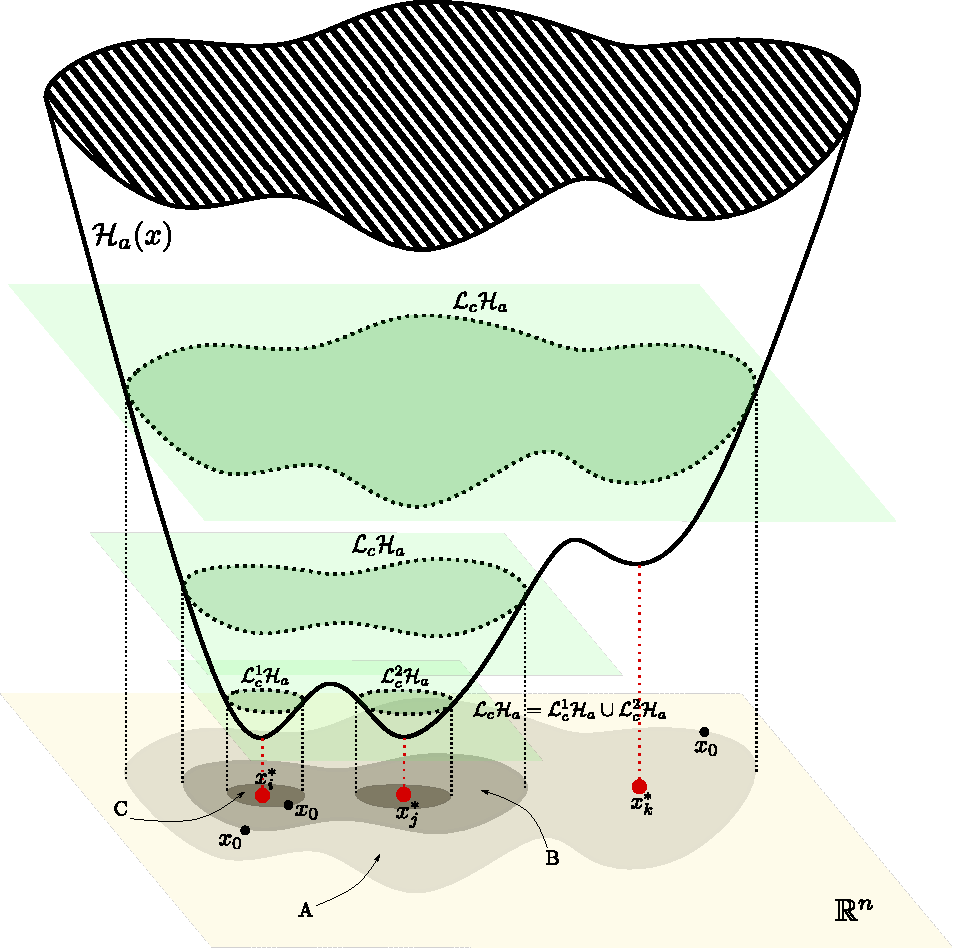
\includegraphics{draw2.pdf}
%	%% This file was created by matlab2tikz.
%
%The latest updates can be retrieved from
%  http://www.mathworks.com/matlabcentral/fileexchange/22022-matlab2tikz-matlab2tikz
%where you can also make suggestions and rate matlab2tikz.
%
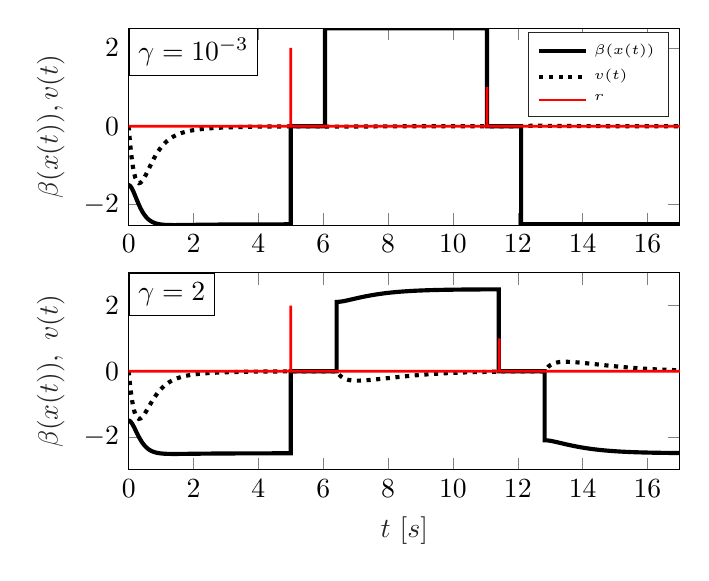
\begin{tikzpicture}

\begin{axis}[%
width=7cm,
height=2.5cm,
at={(0.758in,0.677in)},
scale only axis,
xmin=0,
xmax=17,
xlabel style={font=\color{white!15!black}},
xlabel={$t~[s]$},
ymin=-3,
ymax=3,
ylabel style={font=\color{white!15!black}},
ylabel={$\beta(x(t)),~v(t)$},
title = {${\gamma = 2}$},
every axis title/.style={below right,at={(0,1)},draw=black,fill=white},
axis background/.style={fill=white},
legend style={legend cell align=left, align=left, draw=white!15!black}
]
\addplot [color=black, line width=1.5pt]
  table[row sep=crcr]{%
0	-1.504\\
0.00201272951242755	-1.5040421239506\\
0.00402545902485509	-1.50416792485845\\
0.00603818853728264	-1.5043765408288\\
0.00805091804971019	-1.50466710296983\\
0.0181145656118479	-1.50731826395972\\
0.0281782131739857	-1.51188437125506\\
0.0382418607361234	-1.51825113419416\\
0.0483055082982611	-1.52630255249421\\
0.0872883339796663	-1.57124666864089\\
0.126271159661072	-1.63307936631001\\
0.165253985342477	-1.70570562615994\\
0.204236811023882	-1.78393666097299\\
0.258325242573133	-1.89406957792454\\
0.312413674122383	-1.99919533366988\\
0.366502105671634	-2.0946063144719\\
0.420590537220884	-2.17791827295709\\
0.481968041514646	-2.25709674809204\\
0.543345545808408	-2.3211017273968\\
0.60472305010217	-2.37177374143069\\
0.666100554395931	-2.41108279191348\\
0.724027870722878	-2.43960124498595\\
0.781955187049825	-2.46149216617405\\
0.839882503376772	-2.47812312445785\\
0.897809819703719	-2.49061320040479\\
0.966381939079961	-2.50129669674163\\
1.0349540584562	-2.50866455721899\\
1.10352617783245	-2.51361634287661\\
1.17209829720869	-2.51682148645407\\
1.24444068335681	-2.51885213351912\\
1.31678306950493	-2.51990312114615\\
1.38912545565305	-2.5202746069692\\
1.46146784180118	-2.52018130440801\\
1.5338102279493	-2.51977333101009\\
1.60615261409742	-2.51915819348171\\
1.67849500024554	-2.51841295850998\\
1.75083738639366	-2.51759034387962\\
1.83596904357362	-2.51657064140258\\
1.92110070075358	-2.51553710306555\\
2.00623235793354	-2.51451904955011\\
2.0913640151135	-2.51353114695333\\
2.18740015096789	-2.51246177380188\\
2.28343628682228	-2.51145317347952\\
2.37947242267667	-2.51051138378251\\
2.47550855853105	-2.50963427705357\\
2.58940334197328	-2.50867195136141\\
2.7032981254155	-2.50779651566838\\
2.81719290885772	-2.50700536225962\\
2.93108769229994	-2.50628926775151\\
3.05608769229994	-2.50557903978726\\
3.18108769229994	-2.50494582761179\\
3.30608769229994	-2.50438373443774\\
3.43108769229994	-2.5038835838969\\
3.55608769229994	-2.50343714479222\\
3.68108769229994	-2.50304104287402\\
3.80608769229994	-2.50269039482711\\
3.93108769229994	-2.50237953701534\\
4.05608769229994	-2.50210344689872\\
4.18108769229994	-2.5018590601567\\
4.30608769229994	-2.50164301703084\\
4.43108769229994	-2.50145185801545\\
4.55608769229994	-2.50128252248831\\
4.68108769229994	-2.50113282266486\\
4.80608769229994	-2.50100058926017\\
4.93108769229994	-2.50088371275499\\
4.94831576922496	-2.50086869645166\\
4.96554384614997	-2.50085393407084\\
4.98277192307499	-2.5008394213574\\
5	-2.50082515412478\\
5	0\\
5.001	0\\
5.002	0\\
5.003	0\\
5.004	0\\
5.005	0\\
5.006	0\\
5.007	0\\
5.008	0\\
5.009	0\\
5.01	0\\
5.011	0\\
5.012	0\\
5.013	0\\
5.014	0\\
5.015	0\\
5.016	0\\
5.017	0\\
5.018	0\\
5.019	0\\
5.02	0\\
5.021	0\\
5.022	0\\
5.023	0\\
5.024	0\\
5.025	0\\
5.026	0\\
5.027	0\\
5.028	0\\
5.029	0\\
5.03	0\\
5.031	0\\
5.032	0\\
5.033	0\\
5.034	0\\
5.035	0\\
5.036	0\\
5.037	0\\
5.038	0\\
5.039	0\\
5.04	0\\
5.041	0\\
5.042	0\\
5.043	0\\
5.044	0\\
5.045	0\\
5.046	0\\
5.047	0\\
5.048	0\\
5.049	0\\
5.05	0\\
5.051	0\\
5.052	0\\
5.053	0\\
5.054	0\\
5.055	0\\
5.056	0\\
5.057	0\\
5.058	0\\
5.059	0\\
5.06	0\\
5.061	0\\
5.062	0\\
5.063	0\\
5.064	0\\
5.065	0\\
5.066	0\\
5.067	0\\
5.068	0\\
5.069	0\\
5.07	0\\
5.071	0\\
5.072	0\\
5.073	0\\
5.074	0\\
5.075	0\\
5.076	0\\
5.077	0\\
5.078	0\\
5.079	0\\
5.08	0\\
5.081	0\\
5.082	0\\
5.083	0\\
5.084	0\\
5.085	0\\
5.086	0\\
5.087	0\\
5.088	0\\
5.089	0\\
5.09	0\\
5.091	0\\
5.092	0\\
5.093	0\\
5.094	0\\
5.095	0\\
5.096	0\\
5.097	0\\
5.098	0\\
5.099	0\\
5.1	0\\
5.101	0\\
5.102	0\\
5.103	0\\
5.104	0\\
5.105	0\\
5.106	0\\
5.107	0\\
5.108	0\\
5.109	0\\
5.11	0\\
5.111	0\\
5.112	0\\
5.113	0\\
5.114	0\\
5.115	0\\
5.116	0\\
5.117	0\\
5.118	0\\
5.119	0\\
5.12	0\\
5.121	0\\
5.122	0\\
5.123	0\\
5.124	0\\
5.125	0\\
5.126	0\\
5.127	0\\
5.128	0\\
5.129	0\\
5.13	0\\
5.131	0\\
5.132	0\\
5.133	0\\
5.134	0\\
5.135	0\\
5.136	0\\
5.137	0\\
5.138	0\\
5.139	0\\
5.14	0\\
5.141	0\\
5.142	0\\
5.143	0\\
5.144	0\\
5.145	0\\
5.146	0\\
5.147	0\\
5.148	0\\
5.149	0\\
5.15	0\\
5.151	0\\
5.152	0\\
5.153	0\\
5.154	0\\
5.155	0\\
5.156	0\\
5.157	0\\
5.158	0\\
5.159	0\\
5.16	0\\
5.161	0\\
5.162	0\\
5.163	0\\
5.164	0\\
5.165	0\\
5.166	0\\
5.167	0\\
5.168	0\\
5.169	0\\
5.17	0\\
5.171	0\\
5.172	0\\
5.173	0\\
5.174	0\\
5.175	0\\
5.176	0\\
5.177	0\\
5.178	0\\
5.179	0\\
5.18	0\\
5.181	0\\
5.182	0\\
5.183	0\\
5.184	0\\
5.185	0\\
5.186	0\\
5.187	0\\
5.188	0\\
5.189	0\\
5.19	0\\
5.191	0\\
5.192	0\\
5.193	0\\
5.194	0\\
5.195	0\\
5.196	0\\
5.197	0\\
5.198	0\\
5.199	0\\
5.2	0\\
5.201	0\\
5.202	0\\
5.203	0\\
5.204	0\\
5.205	0\\
5.206	0\\
5.207	0\\
5.208	0\\
5.209	0\\
5.21	0\\
5.211	0\\
5.212	0\\
5.213	0\\
5.214	0\\
5.215	0\\
5.216	0\\
5.217	0\\
5.218	0\\
5.219	0\\
5.22	0\\
5.221	0\\
5.222	0\\
5.223	0\\
5.224	0\\
5.225	0\\
5.226	0\\
5.227	0\\
5.228	0\\
5.229	0\\
5.23	0\\
5.231	0\\
5.232	0\\
5.233	0\\
5.234	0\\
5.235	0\\
5.236	0\\
5.237	0\\
5.238	0\\
5.239	0\\
5.24	0\\
5.241	0\\
5.242	0\\
5.243	0\\
5.244	0\\
5.245	0\\
5.246	0\\
5.247	0\\
5.248	0\\
5.249	0\\
5.25	0\\
5.251	0\\
5.252	0\\
5.253	0\\
5.254	0\\
5.255	0\\
5.256	0\\
5.257	0\\
5.258	0\\
5.259	0\\
5.26	0\\
5.261	0\\
5.262	0\\
5.263	0\\
5.264	0\\
5.265	0\\
5.266	0\\
5.267	0\\
5.268	0\\
5.269	0\\
5.27	0\\
5.271	0\\
5.272	0\\
5.273	0\\
5.274	0\\
5.275	0\\
5.276	0\\
5.277	0\\
5.278	0\\
5.279	0\\
5.28	0\\
5.281	0\\
5.282	0\\
5.283	0\\
5.284	0\\
5.285	0\\
5.286	0\\
5.287	0\\
5.288	0\\
5.289	0\\
5.29	0\\
5.291	0\\
5.292	0\\
5.293	0\\
5.294	0\\
5.295	0\\
5.296	0\\
5.297	0\\
5.298	0\\
5.299	0\\
5.3	0\\
5.301	0\\
5.302	0\\
5.303	0\\
5.304	0\\
5.305	0\\
5.306	0\\
5.307	0\\
5.308	0\\
5.309	0\\
5.31	0\\
5.311	0\\
5.312	0\\
5.313	0\\
5.314	0\\
5.315	0\\
5.316	0\\
5.317	0\\
5.318	0\\
5.319	0\\
5.32	0\\
5.321	0\\
5.322	0\\
5.323	0\\
5.324	0\\
5.325	0\\
5.326	0\\
5.327	0\\
5.328	0\\
5.329	0\\
5.33	0\\
5.331	0\\
5.332	0\\
5.333	0\\
5.334	0\\
5.335	0\\
5.336	0\\
5.337	0\\
5.338	0\\
5.339	0\\
5.34	0\\
5.341	0\\
5.342	0\\
5.343	0\\
5.344	0\\
5.345	0\\
5.346	0\\
5.347	0\\
5.348	0\\
5.349	0\\
5.35	0\\
5.351	0\\
5.352	0\\
5.353	0\\
5.354	0\\
5.355	0\\
5.356	0\\
5.357	0\\
5.358	0\\
5.359	0\\
5.36	0\\
5.361	0\\
5.362	0\\
5.363	0\\
5.364	0\\
5.365	0\\
5.366	0\\
5.367	0\\
5.368	0\\
5.369	0\\
5.37	0\\
5.371	0\\
5.372	0\\
5.373	0\\
5.374	0\\
5.375	0\\
5.376	0\\
5.377	0\\
5.378	0\\
5.379	0\\
5.38	0\\
5.381	0\\
5.382	0\\
5.383	0\\
5.384	0\\
5.385	0\\
5.386	0\\
5.387	0\\
5.388	0\\
5.389	0\\
5.39	0\\
5.391	0\\
5.392	0\\
5.393	0\\
5.394	0\\
5.395	0\\
5.396	0\\
5.397	0\\
5.398	0\\
5.399	0\\
5.4	0\\
5.401	0\\
5.402	0\\
5.403	0\\
5.404	0\\
5.405	0\\
5.406	0\\
5.407	0\\
5.408	0\\
5.409	0\\
5.41	0\\
5.411	0\\
5.412	0\\
5.413	0\\
5.414	0\\
5.415	0\\
5.416	0\\
5.417	0\\
5.418	0\\
5.419	0\\
5.42	0\\
5.421	0\\
5.422	0\\
5.423	0\\
5.424	0\\
5.425	0\\
5.426	0\\
5.427	0\\
5.428	0\\
5.429	0\\
5.43	0\\
5.431	0\\
5.432	0\\
5.433	0\\
5.434	0\\
5.435	0\\
5.436	0\\
5.437	0\\
5.438	0\\
5.439	0\\
5.44	0\\
5.441	0\\
5.442	0\\
5.443	0\\
5.444	0\\
5.445	0\\
5.446	0\\
5.447	0\\
5.448	0\\
5.449	0\\
5.45	0\\
5.451	0\\
5.452	0\\
5.453	0\\
5.454	0\\
5.455	0\\
5.456	0\\
5.457	0\\
5.458	0\\
5.459	0\\
5.46	0\\
5.461	0\\
5.462	0\\
5.463	0\\
5.464	0\\
5.465	0\\
5.466	0\\
5.467	0\\
5.468	0\\
5.469	0\\
5.47	0\\
5.471	0\\
5.472	0\\
5.473	0\\
5.474	0\\
5.475	0\\
5.476	0\\
5.477	0\\
5.478	0\\
5.479	0\\
5.48	0\\
5.481	0\\
5.482	0\\
5.483	0\\
5.484	0\\
5.485	0\\
5.486	0\\
5.487	0\\
5.488	0\\
5.489	0\\
5.49	0\\
5.491	0\\
5.492	0\\
5.493	0\\
5.494	0\\
5.495	0\\
5.496	0\\
5.497	0\\
5.498	0\\
5.499	0\\
5.5	0\\
5.501	0\\
5.502	0\\
5.503	0\\
5.504	0\\
5.505	0\\
5.506	0\\
5.507	0\\
5.508	0\\
5.509	0\\
5.51	0\\
5.511	0\\
5.512	0\\
5.513	0\\
5.514	0\\
5.515	0\\
5.516	0\\
5.517	0\\
5.518	0\\
5.519	0\\
5.52	0\\
5.521	0\\
5.522	0\\
5.523	0\\
5.524	0\\
5.525	0\\
5.526	0\\
5.527	0\\
5.528	0\\
5.529	0\\
5.53	0\\
5.531	0\\
5.532	0\\
5.533	0\\
5.534	0\\
5.535	0\\
5.536	0\\
5.537	0\\
5.538	0\\
5.539	0\\
5.54	0\\
5.541	0\\
5.542	0\\
5.543	0\\
5.544	0\\
5.545	0\\
5.546	0\\
5.547	0\\
5.548	0\\
5.549	0\\
5.55	0\\
5.551	0\\
5.552	0\\
5.553	0\\
5.554	0\\
5.555	0\\
5.556	0\\
5.557	0\\
5.558	0\\
5.559	0\\
5.56	0\\
5.561	0\\
5.562	0\\
5.563	0\\
5.564	0\\
5.565	0\\
5.566	0\\
5.567	0\\
5.568	0\\
5.569	0\\
5.57	0\\
5.571	0\\
5.572	0\\
5.573	0\\
5.574	0\\
5.575	0\\
5.576	0\\
5.577	0\\
5.578	0\\
5.579	0\\
5.58	0\\
5.581	0\\
5.582	0\\
5.583	0\\
5.584	0\\
5.585	0\\
5.586	0\\
5.587	0\\
5.588	0\\
5.589	0\\
5.59	0\\
5.591	0\\
5.592	0\\
5.593	0\\
5.594	0\\
5.595	0\\
5.596	0\\
5.597	0\\
5.598	0\\
5.599	0\\
5.6	0\\
5.601	0\\
5.602	0\\
5.603	0\\
5.604	0\\
5.605	0\\
5.606	0\\
5.607	0\\
5.608	0\\
5.609	0\\
5.61	0\\
5.611	0\\
5.612	0\\
5.613	0\\
5.614	0\\
5.615	0\\
5.616	0\\
5.617	0\\
5.618	0\\
5.619	0\\
5.62	0\\
5.621	0\\
5.622	0\\
5.623	0\\
5.624	0\\
5.625	0\\
5.626	0\\
5.627	0\\
5.628	0\\
5.629	0\\
5.63	0\\
5.631	0\\
5.632	0\\
5.633	0\\
5.634	0\\
5.635	0\\
5.636	0\\
5.637	0\\
5.638	0\\
5.639	0\\
5.64	0\\
5.641	0\\
5.642	0\\
5.643	0\\
5.644	0\\
5.645	0\\
5.646	0\\
5.647	0\\
5.648	0\\
5.649	0\\
5.65	0\\
5.651	0\\
5.652	0\\
5.653	0\\
5.654	0\\
5.655	0\\
5.656	0\\
5.657	0\\
5.658	0\\
5.659	0\\
5.66	0\\
5.661	0\\
5.662	0\\
5.663	0\\
5.664	0\\
5.665	0\\
5.666	0\\
5.667	0\\
5.668	0\\
5.669	0\\
5.67	0\\
5.671	0\\
5.672	0\\
5.673	0\\
5.674	0\\
5.675	0\\
5.676	0\\
5.677	0\\
5.678	0\\
5.679	0\\
5.68	0\\
5.681	0\\
5.682	0\\
5.683	0\\
5.684	0\\
5.685	0\\
5.686	0\\
5.687	0\\
5.688	0\\
5.689	0\\
5.69	0\\
5.691	0\\
5.692	0\\
5.693	0\\
5.694	0\\
5.695	0\\
5.696	0\\
5.697	0\\
5.698	0\\
5.699	0\\
5.7	0\\
5.701	0\\
5.702	0\\
5.703	0\\
5.704	0\\
5.705	0\\
5.706	0\\
5.707	0\\
5.708	0\\
5.709	0\\
5.71	0\\
5.711	0\\
5.712	0\\
5.713	0\\
5.714	0\\
5.715	0\\
5.716	0\\
5.717	0\\
5.718	0\\
5.719	0\\
5.72	0\\
5.721	0\\
5.722	0\\
5.723	0\\
5.724	0\\
5.725	0\\
5.726	0\\
5.727	0\\
5.728	0\\
5.729	0\\
5.73	0\\
5.731	0\\
5.732	0\\
5.733	0\\
5.734	0\\
5.735	0\\
5.736	0\\
5.737	0\\
5.738	0\\
5.739	0\\
5.74	0\\
5.741	0\\
5.742	0\\
5.743	0\\
5.744	0\\
5.745	0\\
5.746	0\\
5.747	0\\
5.748	0\\
5.749	0\\
5.75	0\\
5.751	0\\
5.752	0\\
5.753	0\\
5.754	0\\
5.755	0\\
5.756	0\\
5.757	0\\
5.758	0\\
5.759	0\\
5.76	0\\
5.761	0\\
5.762	0\\
5.763	0\\
5.764	0\\
5.765	0\\
5.766	0\\
5.767	0\\
5.768	0\\
5.769	0\\
5.77	0\\
5.771	0\\
5.772	0\\
5.773	0\\
5.774	0\\
5.775	0\\
5.776	0\\
5.777	0\\
5.778	0\\
5.779	0\\
5.78	0\\
5.781	0\\
5.782	0\\
5.783	0\\
5.784	0\\
5.785	0\\
5.786	0\\
5.787	0\\
5.788	0\\
5.789	0\\
5.79	0\\
5.791	0\\
5.792	0\\
5.793	0\\
5.794	0\\
5.795	0\\
5.796	0\\
5.797	0\\
5.798	0\\
5.799	0\\
5.8	0\\
5.801	0\\
5.802	0\\
5.803	0\\
5.804	0\\
5.805	0\\
5.806	0\\
5.807	0\\
5.808	0\\
5.809	0\\
5.81	0\\
5.811	0\\
5.812	0\\
5.813	0\\
5.814	0\\
5.815	0\\
5.816	0\\
5.817	0\\
5.818	0\\
5.819	0\\
5.82	0\\
5.821	0\\
5.822	0\\
5.823	0\\
5.824	0\\
5.825	0\\
5.826	0\\
5.827	0\\
5.828	0\\
5.829	0\\
5.83	0\\
5.831	0\\
5.832	0\\
5.833	0\\
5.834	0\\
5.835	0\\
5.836	0\\
5.837	0\\
5.838	0\\
5.839	0\\
5.84	0\\
5.841	0\\
5.842	0\\
5.843	0\\
5.844	0\\
5.845	0\\
5.846	0\\
5.847	0\\
5.848	0\\
5.849	0\\
5.85	0\\
5.851	0\\
5.852	0\\
5.853	0\\
5.854	0\\
5.855	0\\
5.856	0\\
5.857	0\\
5.858	0\\
5.859	0\\
5.86	0\\
5.861	0\\
5.862	0\\
5.863	0\\
5.864	0\\
5.865	0\\
5.866	0\\
5.867	0\\
5.868	0\\
5.869	0\\
5.87	0\\
5.871	0\\
5.872	0\\
5.873	0\\
5.874	0\\
5.875	0\\
5.876	0\\
5.877	0\\
5.878	0\\
5.879	0\\
5.88	0\\
5.881	0\\
5.882	0\\
5.883	0\\
5.884	0\\
5.885	0\\
5.886	0\\
5.887	0\\
5.888	0\\
5.889	0\\
5.89	0\\
5.891	0\\
5.892	0\\
5.893	0\\
5.894	0\\
5.895	0\\
5.896	0\\
5.897	0\\
5.898	0\\
5.899	0\\
5.9	0\\
5.901	0\\
5.902	0\\
5.903	0\\
5.904	0\\
5.905	0\\
5.906	0\\
5.907	0\\
5.908	0\\
5.909	0\\
5.91	0\\
5.911	0\\
5.912	0\\
5.913	0\\
5.914	0\\
5.915	0\\
5.916	0\\
5.917	0\\
5.918	0\\
5.919	0\\
5.92	0\\
5.921	0\\
5.922	0\\
5.923	0\\
5.924	0\\
5.925	0\\
5.926	0\\
5.927	0\\
5.928	0\\
5.929	0\\
5.93	0\\
5.931	0\\
5.932	0\\
5.933	0\\
5.934	0\\
5.935	0\\
5.936	0\\
5.937	0\\
5.938	0\\
5.939	0\\
5.94	0\\
5.941	0\\
5.942	0\\
5.943	0\\
5.944	0\\
5.945	0\\
5.946	0\\
5.947	0\\
5.948	0\\
5.949	0\\
5.95	0\\
5.951	0\\
5.952	0\\
5.953	0\\
5.954	0\\
5.955	0\\
5.956	0\\
5.957	0\\
5.958	0\\
5.959	0\\
5.96	0\\
5.961	0\\
5.962	0\\
5.963	0\\
5.964	0\\
5.965	0\\
5.966	0\\
5.967	0\\
5.968	0\\
5.969	0\\
5.97	0\\
5.971	0\\
5.972	0\\
5.973	0\\
5.974	0\\
5.975	0\\
5.976	0\\
5.977	0\\
5.978	0\\
5.979	0\\
5.98	0\\
5.981	0\\
5.982	0\\
5.983	0\\
5.984	0\\
5.985	0\\
5.986	0\\
5.987	0\\
5.988	0\\
5.989	0\\
5.99	0\\
5.991	0\\
5.992	0\\
5.993	0\\
5.994	0\\
5.995	0\\
5.996	0\\
5.997	0\\
5.998	0\\
5.999	0\\
6	0\\
6.001	0\\
6.002	0\\
6.003	0\\
6.004	0\\
6.005	0\\
6.006	0\\
6.007	0\\
6.008	0\\
6.009	0\\
6.01	0\\
6.011	0\\
6.012	0\\
6.013	0\\
6.014	0\\
6.015	0\\
6.016	0\\
6.017	0\\
6.018	0\\
6.019	0\\
6.02	0\\
6.021	0\\
6.022	0\\
6.023	0\\
6.024	0\\
6.025	0\\
6.026	0\\
6.027	0\\
6.028	0\\
6.029	0\\
6.03	0\\
6.031	0\\
6.032	0\\
6.033	0\\
6.034	0\\
6.035	0\\
6.036	0\\
6.037	0\\
6.038	0\\
6.039	0\\
6.04	0\\
6.041	0\\
6.042	0\\
6.043	0\\
6.044	0\\
6.045	0\\
6.046	0\\
6.047	0\\
6.048	0\\
6.049	0\\
6.05	0\\
6.051	0\\
6.052	0\\
6.053	0\\
6.054	0\\
6.055	0\\
6.056	0\\
6.057	0\\
6.058	0\\
6.059	0\\
6.06	0\\
6.061	0\\
6.062	0\\
6.063	0\\
6.064	0\\
6.065	0\\
6.066	0\\
6.067	0\\
6.068	0\\
6.069	0\\
6.07	0\\
6.071	0\\
6.072	0\\
6.073	0\\
6.074	0\\
6.075	0\\
6.076	0\\
6.077	0\\
6.078	0\\
6.079	0\\
6.08	0\\
6.081	0\\
6.082	0\\
6.083	0\\
6.084	0\\
6.085	0\\
6.086	0\\
6.087	0\\
6.088	0\\
6.089	0\\
6.09	0\\
6.091	0\\
6.092	0\\
6.093	0\\
6.094	0\\
6.095	0\\
6.096	0\\
6.097	0\\
6.098	0\\
6.099	0\\
6.1	0\\
6.101	0\\
6.102	0\\
6.103	0\\
6.104	0\\
6.105	0\\
6.106	0\\
6.107	0\\
6.108	0\\
6.109	0\\
6.11	0\\
6.111	0\\
6.112	0\\
6.113	0\\
6.114	0\\
6.115	0\\
6.116	0\\
6.117	0\\
6.118	0\\
6.119	0\\
6.12	0\\
6.121	0\\
6.122	0\\
6.123	0\\
6.124	0\\
6.125	0\\
6.126	0\\
6.127	0\\
6.128	0\\
6.129	0\\
6.13	0\\
6.131	0\\
6.132	0\\
6.133	0\\
6.134	0\\
6.135	0\\
6.136	0\\
6.137	0\\
6.138	0\\
6.139	0\\
6.14	0\\
6.141	0\\
6.142	0\\
6.143	0\\
6.144	0\\
6.145	0\\
6.146	0\\
6.147	0\\
6.148	0\\
6.149	0\\
6.15	0\\
6.151	0\\
6.152	0\\
6.153	0\\
6.154	0\\
6.155	0\\
6.156	0\\
6.157	0\\
6.158	0\\
6.159	0\\
6.16	0\\
6.161	0\\
6.162	0\\
6.163	0\\
6.164	0\\
6.165	0\\
6.166	0\\
6.167	0\\
6.168	0\\
6.169	0\\
6.17	0\\
6.171	0\\
6.172	0\\
6.173	0\\
6.174	0\\
6.175	0\\
6.176	0\\
6.177	0\\
6.178	0\\
6.179	0\\
6.18	0\\
6.181	0\\
6.182	0\\
6.183	0\\
6.184	0\\
6.185	0\\
6.186	0\\
6.187	0\\
6.188	0\\
6.189	0\\
6.19	0\\
6.191	0\\
6.192	0\\
6.193	0\\
6.194	0\\
6.195	0\\
6.196	0\\
6.197	0\\
6.198	0\\
6.199	0\\
6.2	0\\
6.201	0\\
6.202	0\\
6.203	0\\
6.204	0\\
6.205	0\\
6.206	0\\
6.207	0\\
6.208	0\\
6.209	0\\
6.21	0\\
6.211	0\\
6.212	0\\
6.213	0\\
6.214	0\\
6.215	0\\
6.216	0\\
6.217	0\\
6.218	0\\
6.219	0\\
6.22	0\\
6.221	0\\
6.222	0\\
6.223	0\\
6.224	0\\
6.225	0\\
6.226	0\\
6.227	0\\
6.228	0\\
6.229	0\\
6.23	0\\
6.231	0\\
6.232	0\\
6.233	0\\
6.234	0\\
6.235	0\\
6.236	0\\
6.237	0\\
6.238	0\\
6.239	0\\
6.24	0\\
6.241	0\\
6.242	0\\
6.243	0\\
6.244	0\\
6.245	0\\
6.246	0\\
6.247	0\\
6.248	0\\
6.249	0\\
6.25	0\\
6.251	0\\
6.252	0\\
6.253	0\\
6.254	0\\
6.255	0\\
6.256	0\\
6.257	0\\
6.258	0\\
6.259	0\\
6.26	0\\
6.261	0\\
6.262	0\\
6.263	0\\
6.264	0\\
6.265	0\\
6.266	0\\
6.267	0\\
6.268	0\\
6.269	0\\
6.27	0\\
6.271	0\\
6.272	0\\
6.273	0\\
6.274	0\\
6.275	0\\
6.276	0\\
6.277	0\\
6.278	0\\
6.279	0\\
6.28	0\\
6.281	0\\
6.282	0\\
6.283	0\\
6.284	0\\
6.285	0\\
6.286	0\\
6.287	0\\
6.288	0\\
6.289	0\\
6.29	0\\
6.291	0\\
6.292	0\\
6.293	0\\
6.294	0\\
6.295	0\\
6.296	0\\
6.297	0\\
6.298	0\\
6.299	0\\
6.3	0\\
6.301	0\\
6.302	0\\
6.303	0\\
6.304	0\\
6.305	0\\
6.306	0\\
6.307	0\\
6.308	0\\
6.309	0\\
6.31	0\\
6.311	0\\
6.312	0\\
6.313	0\\
6.314	0\\
6.315	0\\
6.316	0\\
6.317	0\\
6.318	0\\
6.319	0\\
6.32	0\\
6.321	0\\
6.322	0\\
6.323	0\\
6.324	0\\
6.325	0\\
6.326	0\\
6.327	0\\
6.328	0\\
6.329	0\\
6.33	0\\
6.331	0\\
6.332	0\\
6.333	0\\
6.334	0\\
6.335	0\\
6.336	0\\
6.337	0\\
6.338	0\\
6.339	0\\
6.34	0\\
6.341	0\\
6.342	0\\
6.343	0\\
6.344	0\\
6.345	0\\
6.346	0\\
6.347	0\\
6.348	0\\
6.349	0\\
6.35	0\\
6.351	0\\
6.352	0\\
6.353	0\\
6.354	0\\
6.355	0\\
6.356	0\\
6.357	0\\
6.358	0\\
6.359	0\\
6.36	0\\
6.361	0\\
6.362	0\\
6.363	0\\
6.364	0\\
6.365	0\\
6.366	0\\
6.367	0\\
6.368	0\\
6.369	0\\
6.37	0\\
6.371	0\\
6.372	0\\
6.373	0\\
6.374	0\\
6.375	0\\
6.376	0\\
6.377	0\\
6.378	0\\
6.379	0\\
6.38	0\\
6.381	0\\
6.382	0\\
6.383	0\\
6.384	0\\
6.385	0\\
6.386	0\\
6.387	0\\
6.388	0\\
6.389	0\\
6.39	0\\
6.391	0\\
6.392	0\\
6.393	0\\
6.394	0\\
6.395	0\\
6.396	0\\
6.397	0\\
6.398	0\\
6.399	0\\
6.4	0\\
6.401	0\\
6.402	0\\
6.403	0\\
6.404	0\\
6.405	0\\
6.406	0\\
6.407	0\\
6.408	0\\
6.409	0\\
6.41	0\\
6.411	0\\
6.412	0\\
6.413	0\\
6.413	2.1139316693639\\
6.42730885570975	2.11412234770866\\
6.44161771141949	2.11458271024684\\
6.45592656712924	2.11529371448898\\
6.47023542283898	2.11623730139078\\
6.51517744734551	2.12051536201303\\
6.56011947185204	2.12647179532107\\
6.60506149635856	2.13374199061386\\
6.65000352086509	2.14199088166887\\
6.69559714700642	2.15108018188364\\
6.74119077314774	2.16071170234008\\
6.78678439928907	2.17072203975994\\
6.8323780254304	2.18096387958857\\
6.88670805540013	2.19330626627053\\
6.94103808536987	2.20568431358523\\
6.99536811533961	2.21799547886423\\
7.04969814530934	2.23014459971016\\
7.11365261721454	2.24413990213848\\
7.17760708911974	2.25775481596045\\
7.24156156102494	2.27094416057966\\
7.30551603293014	2.28366181904244\\
7.38197671782709	2.29820259589554\\
7.45843740272405	2.31202215669435\\
7.53489808762101	2.32512097853371\\
7.61135877251796	2.33749059854897\\
7.70134213864231	2.35111319564808\\
7.79132550476665	2.36377548890919\\
7.881308870891	2.37552126397596\\
7.97129223701534	2.38637583335275\\
8.0720438339047	2.39750761836149\\
8.17279543079405	2.40764965442173\\
8.2735470276834	2.41687774399794\\
8.37429862457275	2.42524102782635\\
8.48225357766335	2.43329893616551\\
8.59020853075395	2.4405259071389\\
8.69816348384455	2.44700551552019\\
8.80611843693515	2.45279324233867\\
8.92128733479583	2.45826485434564\\
9.03645623265651	2.46310783902498\\
9.15162513051719	2.46739810847239\\
9.26679402837787	2.47118562009055\\
9.39145950708824	2.47477211193423\\
9.5161249857986	2.47790727384046\\
9.64079046450896	2.48065387234801\\
9.76545594321933	2.48305175466436\\
9.89045594321933	2.48514257981024\\
10.0154559432193	2.48697055340701\\
10.1404559432193	2.48857224898578\\
10.2654559432193	2.48997245973096\\
10.3904559432193	2.49119341101114\\
10.5154559432193	2.49226286926307\\
10.6404559432193	2.49320134333166\\
10.7654559432193	2.49402372946499\\
10.8904559432193	2.49474323306017\\
11.0154559432193	2.49537478040974\\
11.1404559432193	2.49592985873586\\
11.2654559432193	2.49641733974889\\
11.3023419574145	2.49654937647319\\
11.3392279716097	2.49667648026421\\
11.3761139858048	2.49679883926087\\
11.413	2.49691663406204\\
11.413	0\\
11.414	0\\
11.415	0\\
11.416	0\\
11.417	0\\
11.418	0\\
11.419	0\\
11.42	0\\
11.421	0\\
11.422	0\\
11.423	0\\
11.424	0\\
11.425	0\\
11.426	0\\
11.427	0\\
11.428	0\\
11.429	0\\
11.43	0\\
11.431	0\\
11.432	0\\
11.433	0\\
11.434	0\\
11.435	0\\
11.436	0\\
11.437	0\\
11.438	0\\
11.439	0\\
11.44	0\\
11.441	0\\
11.442	0\\
11.443	0\\
11.444	0\\
11.445	0\\
11.446	0\\
11.447	0\\
11.448	0\\
11.449	0\\
11.45	0\\
11.451	0\\
11.452	0\\
11.453	0\\
11.454	0\\
11.455	0\\
11.456	0\\
11.457	0\\
11.458	0\\
11.459	0\\
11.46	0\\
11.461	0\\
11.462	0\\
11.463	0\\
11.464	0\\
11.465	0\\
11.466	0\\
11.467	0\\
11.468	0\\
11.469	0\\
11.47	0\\
11.471	0\\
11.472	0\\
11.473	0\\
11.474	0\\
11.475	0\\
11.476	0\\
11.477	0\\
11.478	0\\
11.479	0\\
11.48	0\\
11.481	0\\
11.482	0\\
11.483	0\\
11.484	0\\
11.485	0\\
11.486	0\\
11.487	0\\
11.488	0\\
11.489	0\\
11.49	0\\
11.491	0\\
11.492	0\\
11.493	0\\
11.494	0\\
11.495	0\\
11.496	0\\
11.497	0\\
11.498	0\\
11.499	0\\
11.5	0\\
11.501	0\\
11.502	0\\
11.503	0\\
11.504	0\\
11.505	0\\
11.506	0\\
11.507	0\\
11.508	0\\
11.509	0\\
11.51	0\\
11.511	0\\
11.512	0\\
11.513	0\\
11.514	0\\
11.515	0\\
11.516	0\\
11.517	0\\
11.518	0\\
11.519	0\\
11.52	0\\
11.521	0\\
11.522	0\\
11.523	0\\
11.524	0\\
11.525	0\\
11.526	0\\
11.527	0\\
11.528	0\\
11.529	0\\
11.53	0\\
11.531	0\\
11.532	0\\
11.533	0\\
11.534	0\\
11.535	0\\
11.536	0\\
11.537	0\\
11.538	0\\
11.539	0\\
11.54	0\\
11.541	0\\
11.542	0\\
11.543	0\\
11.544	0\\
11.545	0\\
11.546	0\\
11.547	0\\
11.548	0\\
11.549	0\\
11.55	0\\
11.551	0\\
11.552	0\\
11.553	0\\
11.554	0\\
11.555	0\\
11.556	0\\
11.557	0\\
11.558	0\\
11.559	0\\
11.56	0\\
11.561	0\\
11.562	0\\
11.563	0\\
11.564	0\\
11.565	0\\
11.566	0\\
11.567	0\\
11.568	0\\
11.569	0\\
11.57	0\\
11.571	0\\
11.572	0\\
11.573	0\\
11.574	0\\
11.575	0\\
11.576	0\\
11.577	0\\
11.578	0\\
11.579	0\\
11.58	0\\
11.581	0\\
11.582	0\\
11.583	0\\
11.584	0\\
11.585	0\\
11.586	0\\
11.587	0\\
11.588	0\\
11.589	0\\
11.59	0\\
11.591	0\\
11.592	0\\
11.593	0\\
11.594	0\\
11.595	0\\
11.596	0\\
11.597	0\\
11.598	0\\
11.599	0\\
11.6	0\\
11.601	0\\
11.602	0\\
11.603	0\\
11.604	0\\
11.605	0\\
11.606	0\\
11.607	0\\
11.608	0\\
11.609	0\\
11.61	0\\
11.611	0\\
11.612	0\\
11.613	0\\
11.614	0\\
11.615	0\\
11.616	0\\
11.617	0\\
11.618	0\\
11.619	0\\
11.62	0\\
11.621	0\\
11.622	0\\
11.623	0\\
11.624	0\\
11.625	0\\
11.626	0\\
11.627	0\\
11.628	0\\
11.629	0\\
11.63	0\\
11.631	0\\
11.632	0\\
11.633	0\\
11.634	0\\
11.635	0\\
11.636	0\\
11.637	0\\
11.638	0\\
11.639	0\\
11.64	0\\
11.641	0\\
11.642	0\\
11.643	0\\
11.644	0\\
11.645	0\\
11.646	0\\
11.647	0\\
11.648	0\\
11.649	0\\
11.65	0\\
11.651	0\\
11.652	0\\
11.653	0\\
11.654	0\\
11.655	0\\
11.656	0\\
11.657	0\\
11.658	0\\
11.659	0\\
11.66	0\\
11.661	0\\
11.662	0\\
11.663	0\\
11.664	0\\
11.665	0\\
11.666	0\\
11.667	0\\
11.668	0\\
11.669	0\\
11.67	0\\
11.671	0\\
11.672	0\\
11.673	0\\
11.674	0\\
11.675	0\\
11.676	0\\
11.677	0\\
11.678	0\\
11.679	0\\
11.68	0\\
11.681	0\\
11.682	0\\
11.683	0\\
11.684	0\\
11.685	0\\
11.686	0\\
11.687	0\\
11.688	0\\
11.689	0\\
11.69	0\\
11.691	0\\
11.692	0\\
11.693	0\\
11.694	0\\
11.695	0\\
11.696	0\\
11.697	0\\
11.698	0\\
11.699	0\\
11.7	0\\
11.701	0\\
11.702	0\\
11.703	0\\
11.704	0\\
11.705	0\\
11.706	0\\
11.707	0\\
11.708	0\\
11.709	0\\
11.71	0\\
11.711	0\\
11.712	0\\
11.713	0\\
11.714	0\\
11.715	0\\
11.716	0\\
11.717	0\\
11.718	0\\
11.719	0\\
11.72	0\\
11.721	0\\
11.722	0\\
11.723	0\\
11.724	0\\
11.725	0\\
11.726	0\\
11.727	0\\
11.728	0\\
11.729	0\\
11.73	0\\
11.731	0\\
11.732	0\\
11.733	0\\
11.734	0\\
11.735	0\\
11.736	0\\
11.737	0\\
11.738	0\\
11.739	0\\
11.74	0\\
11.741	0\\
11.742	0\\
11.743	0\\
11.744	0\\
11.745	0\\
11.746	0\\
11.747	0\\
11.748	0\\
11.749	0\\
11.75	0\\
11.751	0\\
11.752	0\\
11.753	0\\
11.754	0\\
11.755	0\\
11.756	0\\
11.757	0\\
11.758	0\\
11.759	0\\
11.76	0\\
11.761	0\\
11.762	0\\
11.763	0\\
11.764	0\\
11.765	0\\
11.766	0\\
11.767	0\\
11.768	0\\
11.769	0\\
11.77	0\\
11.771	0\\
11.772	0\\
11.773	0\\
11.774	0\\
11.775	0\\
11.776	0\\
11.777	0\\
11.778	0\\
11.779	0\\
11.78	0\\
11.781	0\\
11.782	0\\
11.783	0\\
11.784	0\\
11.785	0\\
11.786	0\\
11.787	0\\
11.788	0\\
11.789	0\\
11.79	0\\
11.791	0\\
11.792	0\\
11.793	0\\
11.794	0\\
11.795	0\\
11.796	0\\
11.797	0\\
11.798	0\\
11.799	0\\
11.8	0\\
11.801	0\\
11.802	0\\
11.803	0\\
11.804	0\\
11.805	0\\
11.806	0\\
11.807	0\\
11.808	0\\
11.809	0\\
11.81	0\\
11.811	0\\
11.812	0\\
11.813	0\\
11.814	0\\
11.815	0\\
11.816	0\\
11.817	0\\
11.818	0\\
11.819	0\\
11.82	0\\
11.821	0\\
11.822	0\\
11.823	0\\
11.824	0\\
11.825	0\\
11.826	0\\
11.827	0\\
11.828	0\\
11.829	0\\
11.83	0\\
11.831	0\\
11.832	0\\
11.833	0\\
11.834	0\\
11.835	0\\
11.836	0\\
11.837	0\\
11.838	0\\
11.839	0\\
11.84	0\\
11.841	0\\
11.842	0\\
11.843	0\\
11.844	0\\
11.845	0\\
11.846	0\\
11.847	0\\
11.848	0\\
11.849	0\\
11.85	0\\
11.851	0\\
11.852	0\\
11.853	0\\
11.854	0\\
11.855	0\\
11.856	0\\
11.857	0\\
11.858	0\\
11.859	0\\
11.86	0\\
11.861	0\\
11.862	0\\
11.863	0\\
11.864	0\\
11.865	0\\
11.866	0\\
11.867	0\\
11.868	0\\
11.869	0\\
11.87	0\\
11.871	0\\
11.872	0\\
11.873	0\\
11.874	0\\
11.875	0\\
11.876	0\\
11.877	0\\
11.878	0\\
11.879	0\\
11.88	0\\
11.881	0\\
11.882	0\\
11.883	0\\
11.884	0\\
11.885	0\\
11.886	0\\
11.887	0\\
11.888	0\\
11.889	0\\
11.89	0\\
11.891	0\\
11.892	0\\
11.893	0\\
11.894	0\\
11.895	0\\
11.896	0\\
11.897	0\\
11.898	0\\
11.899	0\\
11.9	0\\
11.901	0\\
11.902	0\\
11.903	0\\
11.904	0\\
11.905	0\\
11.906	0\\
11.907	0\\
11.908	0\\
11.909	0\\
11.91	0\\
11.911	0\\
11.912	0\\
11.913	0\\
11.914	0\\
11.915	0\\
11.916	0\\
11.917	0\\
11.918	0\\
11.919	0\\
11.92	0\\
11.921	0\\
11.922	0\\
11.923	0\\
11.924	0\\
11.925	0\\
11.926	0\\
11.927	0\\
11.928	0\\
11.929	0\\
11.93	0\\
11.931	0\\
11.932	0\\
11.933	0\\
11.934	0\\
11.935	0\\
11.936	0\\
11.937	0\\
11.938	0\\
11.939	0\\
11.94	0\\
11.941	0\\
11.942	0\\
11.943	0\\
11.944	0\\
11.945	0\\
11.946	0\\
11.947	0\\
11.948	0\\
11.949	0\\
11.95	0\\
11.951	0\\
11.952	0\\
11.953	0\\
11.954	0\\
11.955	0\\
11.956	0\\
11.957	0\\
11.958	0\\
11.959	0\\
11.96	0\\
11.961	0\\
11.962	0\\
11.963	0\\
11.964	0\\
11.965	0\\
11.966	0\\
11.967	0\\
11.968	0\\
11.969	0\\
11.97	0\\
11.971	0\\
11.972	0\\
11.973	0\\
11.974	0\\
11.975	0\\
11.976	0\\
11.977	0\\
11.978	0\\
11.979	0\\
11.98	0\\
11.981	0\\
11.982	0\\
11.983	0\\
11.984	0\\
11.985	0\\
11.986	0\\
11.987	0\\
11.988	0\\
11.989	0\\
11.99	0\\
11.991	0\\
11.992	0\\
11.993	0\\
11.994	0\\
11.995	0\\
11.996	0\\
11.997	0\\
11.998	0\\
11.999	0\\
12	0\\
12.001	0\\
12.002	0\\
12.003	0\\
12.004	0\\
12.005	0\\
12.006	0\\
12.007	0\\
12.008	0\\
12.009	0\\
12.01	0\\
12.011	0\\
12.012	0\\
12.013	0\\
12.014	0\\
12.015	0\\
12.016	0\\
12.017	0\\
12.018	0\\
12.019	0\\
12.02	0\\
12.021	0\\
12.022	0\\
12.023	0\\
12.024	0\\
12.025	0\\
12.026	0\\
12.027	0\\
12.028	0\\
12.029	0\\
12.03	0\\
12.031	0\\
12.032	0\\
12.033	0\\
12.034	0\\
12.035	0\\
12.036	0\\
12.037	0\\
12.038	0\\
12.039	0\\
12.04	0\\
12.041	0\\
12.042	0\\
12.043	0\\
12.044	0\\
12.045	0\\
12.046	0\\
12.047	0\\
12.048	0\\
12.049	0\\
12.05	0\\
12.051	0\\
12.052	0\\
12.053	0\\
12.054	0\\
12.055	0\\
12.056	0\\
12.057	0\\
12.058	0\\
12.059	0\\
12.06	0\\
12.061	0\\
12.062	0\\
12.063	0\\
12.064	0\\
12.065	0\\
12.066	0\\
12.067	0\\
12.068	0\\
12.069	0\\
12.07	0\\
12.071	0\\
12.072	0\\
12.073	0\\
12.074	0\\
12.075	0\\
12.076	0\\
12.077	0\\
12.078	0\\
12.079	0\\
12.08	0\\
12.081	0\\
12.082	0\\
12.083	0\\
12.084	0\\
12.085	0\\
12.086	0\\
12.087	0\\
12.088	0\\
12.089	0\\
12.09	0\\
12.091	0\\
12.092	0\\
12.093	0\\
12.094	0\\
12.095	0\\
12.096	0\\
12.097	0\\
12.098	0\\
12.099	0\\
12.1	0\\
12.101	0\\
12.102	0\\
12.103	0\\
12.104	0\\
12.105	0\\
12.106	0\\
12.107	0\\
12.108	0\\
12.109	0\\
12.11	0\\
12.111	0\\
12.112	0\\
12.113	0\\
12.114	0\\
12.115	0\\
12.116	0\\
12.117	0\\
12.118	0\\
12.119	0\\
12.12	0\\
12.121	0\\
12.122	0\\
12.123	0\\
12.124	0\\
12.125	0\\
12.126	0\\
12.127	0\\
12.128	0\\
12.129	0\\
12.13	0\\
12.131	0\\
12.132	0\\
12.133	0\\
12.134	0\\
12.135	0\\
12.136	0\\
12.137	0\\
12.138	0\\
12.139	0\\
12.14	0\\
12.141	0\\
12.142	0\\
12.143	0\\
12.144	0\\
12.145	0\\
12.146	0\\
12.147	0\\
12.148	0\\
12.149	0\\
12.15	0\\
12.151	0\\
12.152	0\\
12.153	0\\
12.154	0\\
12.155	0\\
12.156	0\\
12.157	0\\
12.158	0\\
12.159	0\\
12.16	0\\
12.161	0\\
12.162	0\\
12.163	0\\
12.164	0\\
12.165	0\\
12.166	0\\
12.167	0\\
12.168	0\\
12.169	0\\
12.17	0\\
12.171	0\\
12.172	0\\
12.173	0\\
12.174	0\\
12.175	0\\
12.176	0\\
12.177	0\\
12.178	0\\
12.179	0\\
12.18	0\\
12.181	0\\
12.182	0\\
12.183	0\\
12.184	0\\
12.185	0\\
12.186	0\\
12.187	0\\
12.188	0\\
12.189	0\\
12.19	0\\
12.191	0\\
12.192	0\\
12.193	0\\
12.194	0\\
12.195	0\\
12.196	0\\
12.197	0\\
12.198	0\\
12.199	0\\
12.2	0\\
12.201	0\\
12.202	0\\
12.203	0\\
12.204	0\\
12.205	0\\
12.206	0\\
12.207	0\\
12.208	0\\
12.209	0\\
12.21	0\\
12.211	0\\
12.212	0\\
12.213	0\\
12.214	0\\
12.215	0\\
12.216	0\\
12.217	0\\
12.218	0\\
12.219	0\\
12.22	0\\
12.221	0\\
12.222	0\\
12.223	0\\
12.224	0\\
12.225	0\\
12.226	0\\
12.227	0\\
12.228	0\\
12.229	0\\
12.23	0\\
12.231	0\\
12.232	0\\
12.233	0\\
12.234	0\\
12.235	0\\
12.236	0\\
12.237	0\\
12.238	0\\
12.239	0\\
12.24	0\\
12.241	0\\
12.242	0\\
12.243	0\\
12.244	0\\
12.245	0\\
12.246	0\\
12.247	0\\
12.248	0\\
12.249	0\\
12.25	0\\
12.251	0\\
12.252	0\\
12.253	0\\
12.254	0\\
12.255	0\\
12.256	0\\
12.257	0\\
12.258	0\\
12.259	0\\
12.26	0\\
12.261	0\\
12.262	0\\
12.263	0\\
12.264	0\\
12.265	0\\
12.266	0\\
12.267	0\\
12.268	0\\
12.269	0\\
12.27	0\\
12.271	0\\
12.272	0\\
12.273	0\\
12.274	0\\
12.275	0\\
12.276	0\\
12.277	0\\
12.278	0\\
12.279	0\\
12.28	0\\
12.281	0\\
12.282	0\\
12.283	0\\
12.284	0\\
12.285	0\\
12.286	0\\
12.287	0\\
12.288	0\\
12.289	0\\
12.29	0\\
12.291	0\\
12.292	0\\
12.293	0\\
12.294	0\\
12.295	0\\
12.296	0\\
12.297	0\\
12.298	0\\
12.299	0\\
12.3	0\\
12.301	0\\
12.302	0\\
12.303	0\\
12.304	0\\
12.305	0\\
12.306	0\\
12.307	0\\
12.308	0\\
12.309	0\\
12.31	0\\
12.311	0\\
12.312	0\\
12.313	0\\
12.314	0\\
12.315	0\\
12.316	0\\
12.317	0\\
12.318	0\\
12.319	0\\
12.32	0\\
12.321	0\\
12.322	0\\
12.323	0\\
12.324	0\\
12.325	0\\
12.326	0\\
12.327	0\\
12.328	0\\
12.329	0\\
12.33	0\\
12.331	0\\
12.332	0\\
12.333	0\\
12.334	0\\
12.335	0\\
12.336	0\\
12.337	0\\
12.338	0\\
12.339	0\\
12.34	0\\
12.341	0\\
12.342	0\\
12.343	0\\
12.344	0\\
12.345	0\\
12.346	0\\
12.347	0\\
12.348	0\\
12.349	0\\
12.35	0\\
12.351	0\\
12.352	0\\
12.353	0\\
12.354	0\\
12.355	0\\
12.356	0\\
12.357	0\\
12.358	0\\
12.359	0\\
12.36	0\\
12.361	0\\
12.362	0\\
12.363	0\\
12.364	0\\
12.365	0\\
12.366	0\\
12.367	0\\
12.368	0\\
12.369	0\\
12.37	0\\
12.371	0\\
12.372	0\\
12.373	0\\
12.374	0\\
12.375	0\\
12.376	0\\
12.377	0\\
12.378	0\\
12.379	0\\
12.38	0\\
12.381	0\\
12.382	0\\
12.383	0\\
12.384	0\\
12.385	0\\
12.386	0\\
12.387	0\\
12.388	0\\
12.389	0\\
12.39	0\\
12.391	0\\
12.392	0\\
12.393	0\\
12.394	0\\
12.395	0\\
12.396	0\\
12.397	0\\
12.398	0\\
12.399	0\\
12.4	0\\
12.401	0\\
12.402	0\\
12.403	0\\
12.404	0\\
12.405	0\\
12.406	0\\
12.407	0\\
12.408	0\\
12.409	0\\
12.41	0\\
12.411	0\\
12.412	0\\
12.413	0\\
12.414	0\\
12.415	0\\
12.416	0\\
12.417	0\\
12.418	0\\
12.419	0\\
12.42	0\\
12.421	0\\
12.422	0\\
12.423	0\\
12.424	0\\
12.425	0\\
12.426	0\\
12.427	0\\
12.428	0\\
12.429	0\\
12.43	0\\
12.431	0\\
12.432	0\\
12.433	0\\
12.434	0\\
12.435	0\\
12.436	0\\
12.437	0\\
12.438	0\\
12.439	0\\
12.44	0\\
12.441	0\\
12.442	0\\
12.443	0\\
12.444	0\\
12.445	0\\
12.446	0\\
12.447	0\\
12.448	0\\
12.449	0\\
12.45	0\\
12.451	0\\
12.452	0\\
12.453	0\\
12.454	0\\
12.455	0\\
12.456	0\\
12.457	0\\
12.458	0\\
12.459	0\\
12.46	0\\
12.461	0\\
12.462	0\\
12.463	0\\
12.464	0\\
12.465	0\\
12.466	0\\
12.467	0\\
12.468	0\\
12.469	0\\
12.47	0\\
12.471	0\\
12.472	0\\
12.473	0\\
12.474	0\\
12.475	0\\
12.476	0\\
12.477	0\\
12.478	0\\
12.479	0\\
12.48	0\\
12.481	0\\
12.482	0\\
12.483	0\\
12.484	0\\
12.485	0\\
12.486	0\\
12.487	0\\
12.488	0\\
12.489	0\\
12.49	0\\
12.491	0\\
12.492	0\\
12.493	0\\
12.494	0\\
12.495	0\\
12.496	0\\
12.497	0\\
12.498	0\\
12.499	0\\
12.5	0\\
12.501	0\\
12.502	0\\
12.503	0\\
12.504	0\\
12.505	0\\
12.506	0\\
12.507	0\\
12.508	0\\
12.509	0\\
12.51	0\\
12.511	0\\
12.512	0\\
12.513	0\\
12.514	0\\
12.515	0\\
12.516	0\\
12.517	0\\
12.518	0\\
12.519	0\\
12.52	0\\
12.521	0\\
12.522	0\\
12.523	0\\
12.524	0\\
12.525	0\\
12.526	0\\
12.527	0\\
12.528	0\\
12.529	0\\
12.53	0\\
12.531	0\\
12.532	0\\
12.533	0\\
12.534	0\\
12.535	0\\
12.536	0\\
12.537	0\\
12.538	0\\
12.539	0\\
12.54	0\\
12.541	0\\
12.542	0\\
12.543	0\\
12.544	0\\
12.545	0\\
12.546	0\\
12.547	0\\
12.548	0\\
12.549	0\\
12.55	0\\
12.551	0\\
12.552	0\\
12.553	0\\
12.554	0\\
12.555	0\\
12.556	0\\
12.557	0\\
12.558	0\\
12.559	0\\
12.56	0\\
12.561	0\\
12.562	0\\
12.563	0\\
12.564	0\\
12.565	0\\
12.566	0\\
12.567	0\\
12.568	0\\
12.569	0\\
12.57	0\\
12.571	0\\
12.572	0\\
12.573	0\\
12.574	0\\
12.575	0\\
12.576	0\\
12.577	0\\
12.578	0\\
12.579	0\\
12.58	0\\
12.581	0\\
12.582	0\\
12.583	0\\
12.584	0\\
12.585	0\\
12.586	0\\
12.587	0\\
12.588	0\\
12.589	0\\
12.59	0\\
12.591	0\\
12.592	0\\
12.593	0\\
12.594	0\\
12.595	0\\
12.596	0\\
12.597	0\\
12.598	0\\
12.599	0\\
12.6	0\\
12.601	0\\
12.602	0\\
12.603	0\\
12.604	0\\
12.605	0\\
12.606	0\\
12.607	0\\
12.608	0\\
12.609	0\\
12.61	0\\
12.611	0\\
12.612	0\\
12.613	0\\
12.614	0\\
12.615	0\\
12.616	0\\
12.617	0\\
12.618	0\\
12.619	0\\
12.62	0\\
12.621	0\\
12.622	0\\
12.623	0\\
12.624	0\\
12.625	0\\
12.626	0\\
12.627	0\\
12.628	0\\
12.629	0\\
12.63	0\\
12.631	0\\
12.632	0\\
12.633	0\\
12.634	0\\
12.635	0\\
12.636	0\\
12.637	0\\
12.638	0\\
12.639	0\\
12.64	0\\
12.641	0\\
12.642	0\\
12.643	0\\
12.644	0\\
12.645	0\\
12.646	0\\
12.647	0\\
12.648	0\\
12.649	0\\
12.65	0\\
12.651	0\\
12.652	0\\
12.653	0\\
12.654	0\\
12.655	0\\
12.656	0\\
12.657	0\\
12.658	0\\
12.659	0\\
12.66	0\\
12.661	0\\
12.662	0\\
12.663	0\\
12.664	0\\
12.665	0\\
12.666	0\\
12.667	0\\
12.668	0\\
12.669	0\\
12.67	0\\
12.671	0\\
12.672	0\\
12.673	0\\
12.674	0\\
12.675	0\\
12.676	0\\
12.677	0\\
12.678	0\\
12.679	0\\
12.68	0\\
12.681	0\\
12.682	0\\
12.683	0\\
12.684	0\\
12.685	0\\
12.686	0\\
12.687	0\\
12.688	0\\
12.689	0\\
12.69	0\\
12.691	0\\
12.692	0\\
12.693	0\\
12.694	0\\
12.695	0\\
12.696	0\\
12.697	0\\
12.698	0\\
12.699	0\\
12.7	0\\
12.701	0\\
12.702	0\\
12.703	0\\
12.704	0\\
12.705	0\\
12.706	0\\
12.707	0\\
12.708	0\\
12.709	0\\
12.71	0\\
12.711	0\\
12.712	0\\
12.713	0\\
12.714	0\\
12.715	0\\
12.716	0\\
12.717	0\\
12.718	0\\
12.719	0\\
12.72	0\\
12.721	0\\
12.722	0\\
12.723	0\\
12.724	0\\
12.725	0\\
12.726	0\\
12.727	0\\
12.728	0\\
12.729	0\\
12.73	0\\
12.731	0\\
12.732	0\\
12.733	0\\
12.734	0\\
12.735	0\\
12.736	0\\
12.737	0\\
12.738	0\\
12.739	0\\
12.74	0\\
12.741	0\\
12.742	0\\
12.743	0\\
12.744	0\\
12.745	0\\
12.746	0\\
12.747	0\\
12.748	0\\
12.749	0\\
12.75	0\\
12.751	0\\
12.752	0\\
12.753	0\\
12.754	0\\
12.755	0\\
12.756	0\\
12.757	0\\
12.758	0\\
12.759	0\\
12.76	0\\
12.761	0\\
12.762	0\\
12.763	0\\
12.764	0\\
12.765	0\\
12.766	0\\
12.767	0\\
12.768	0\\
12.769	0\\
12.77	0\\
12.771	0\\
12.772	0\\
12.773	0\\
12.774	0\\
12.775	0\\
12.776	0\\
12.777	0\\
12.778	0\\
12.779	0\\
12.78	0\\
12.781	0\\
12.782	0\\
12.783	0\\
12.784	0\\
12.785	0\\
12.786	0\\
12.787	0\\
12.788	0\\
12.789	0\\
12.79	0\\
12.791	0\\
12.792	0\\
12.793	0\\
12.794	0\\
12.795	0\\
12.796	0\\
12.797	0\\
12.798	0\\
12.799	0\\
12.8	0\\
12.801	0\\
12.802	0\\
12.803	0\\
12.804	0\\
12.805	0\\
12.806	0\\
12.807	0\\
12.808	0\\
12.809	0\\
12.81	0\\
12.811	0\\
12.812	0\\
12.813	0\\
12.814	0\\
12.815	0\\
12.816	0\\
12.817	0\\
12.818	0\\
12.819	0\\
12.82	0\\
12.821	0\\
12.822	0\\
12.823	0\\
12.824	0\\
12.825	0\\
12.826	0\\
12.827	0\\
12.828	0\\
12.828	-2.1030892188172\\
12.842047021386	-2.10323261303505\\
12.8560940427719	-2.10364411440539\\
12.8701410641579	-2.10430518229921\\
12.8841880855439	-2.10519821856765\\
12.9289290829934	-2.10938882140525\\
12.9736700804429	-2.11530772217348\\
13.0184110778924	-2.12258313999245\\
13.0631520753419	-2.13087329614986\\
13.1084892291656	-2.14002445544475\\
13.1538263829893	-2.14974350147083\\
13.199163536813	-2.15986356496462\\
13.2445006906367	-2.17023414330765\\
13.2985059417722	-2.18274646603771\\
13.3525111929078	-2.19531389481917\\
13.4065164440434	-2.20783082184725\\
13.460521695179	-2.22019923723202\\
13.5240695570875	-2.2344613106829\\
13.5876174189961	-2.2483556089919\\
13.6511652809046	-2.26183428275482\\
13.7147131428131	-2.27484869200743\\
13.7906838958888	-2.28975016452194\\
13.8666546489646	-2.30393495975269\\
13.9426254020403	-2.317400851123\\
14.0185961551161	-2.33013681010178\\
14.1080563635861	-2.34419459286555\\
14.1975165720561	-2.35728388313098\\
14.2869767805262	-2.36944600626342\\
14.3764369889962	-2.38070394244363\\
14.4766543807337	-2.39227516621004\\
14.5768717724713	-2.40283533111701\\
14.6770891642088	-2.4124591677568\\
14.7773065559463	-2.42119465979249\\
14.8845892810493	-2.42961698618916\\
14.9918720061523	-2.43718267161224\\
15.0991547312552	-2.44397577961747\\
15.2064374563582	-2.45005201251652\\
15.320673400412	-2.45579424888234\\
15.4349093444657	-2.46088432602407\\
15.5491452885194	-2.46539952792632\\
15.6633812325732	-2.46939083883895\\
15.7867630527359	-2.47316762515648\\
15.9101448728985	-2.47647401052371\\
16.0335266930612	-2.47937442227392\\
16.1569085132239	-2.48190999102097\\
16.2819085132239	-2.48414532514259\\
16.4069085132239	-2.48609928401365\\
16.5319085132239	-2.48781109853873\\
16.6569085132239	-2.48930715861819\\
16.7819085132239	-2.49061115966788\\
16.9069085132239	-2.49175306118141\\
17.0319085132239	-2.4927548983235\\
17.1569085132239	-2.49363254916976\\
17.2819085132239	-2.49440010128261\\
17.4069085132239	-2.49507365752084\\
17.5319085132239	-2.49566554883437\\
17.6569085132239	-2.49618523285505\\
17.6996813849179	-2.49634792814719\\
17.7424542566119	-2.49650358597675\\
17.785227128306	-2.4966525173879\\
17.828	-2.49679501877743\\
};
%\addlegendentry{$\beta(x(t))$}

\addplot [color=black, dotted, line width=1.5pt]
  table[row sep=crcr]{%
0	-0\\
0.00201272951242755	-0.0224934012716354\\
0.00402545902485509	-0.0447603608414621\\
0.00603818853728264	-0.0668019471809352\\
0.00805091804971019	-0.0886192303459318\\
0.0181145656118479	-0.194378599396095\\
0.0281782131739857	-0.294691894777697\\
0.0382418607361234	-0.389694884662672\\
0.0483055082982611	-0.479524211806853\\
0.0872883339796663	-0.781184325738566\\
0.126271159661072	-1.01538378523468\\
0.165253985342477	-1.19025921656498\\
0.204236811023882	-1.31386886754089\\
0.258325242573133	-1.41500689215222\\
0.312413674122383	-1.45090376204154\\
0.366502105671634	-1.43790632239675\\
0.420590537220884	-1.39062405810714\\
0.481968041514646	-1.31050445125631\\
0.543345545808408	-1.21330641207034\\
0.60472305010217	-1.10814574794384\\
0.666100554395931	-1.00226495239739\\
0.724027870722878	-0.905975517804747\\
0.781955187049825	-0.815045626456067\\
0.839882503376772	-0.730713006605808\\
0.897809819703719	-0.653718196410737\\
0.966381939079961	-0.572237895798701\\
1.0349540584562	-0.500710539966942\\
1.10352617783245	-0.438418039951862\\
1.17209829720869	-0.384478986959469\\
1.24444068335681	-0.335485761815119\\
1.31678306950493	-0.293608722977863\\
1.38912545565305	-0.257906090907107\\
1.46146784180118	-0.22738078186836\\
1.5338102279493	-0.201125079495263\\
1.60615261409742	-0.178579197726964\\
1.67849500024554	-0.159208999476834\\
1.75083738639366	-0.142457053438271\\
1.83596904357362	-0.125436753367043\\
1.92110070075358	-0.110951392981477\\
2.00623235793354	-0.0986182716301151\\
2.0913640151135	-0.0879870970793011\\
2.18740015096789	-0.0775679510309611\\
2.28343628682228	-0.0686499906350762\\
2.37947242267667	-0.0610228399028308\\
2.47550855853105	-0.054401980939246\\
2.58940334197328	-0.047531048507626\\
2.7032981254155	-0.0416624252134102\\
2.81719290885772	-0.0366745685749607\\
2.93108769229994	-0.0323547550007202\\
3.05608769229994	-0.0281814385322176\\
3.18108769229994	-0.0245985646826315\\
3.30608769229994	-0.0215402853793202\\
3.43108769229994	-0.018887855942097\\
3.55608769229994	-0.0165467072979763\\
3.68108769229994	-0.0145124020998248\\
3.80608769229994	-0.0127502632885634\\
3.93108769229994	-0.0112103371224297\\
4.05608769229994	-0.00985157237573263\\
4.18108769229994	-0.0086630171814539\\
4.30608769229994	-0.00762523169470833\\
4.43108769229994	-0.00671453923178449\\
4.55608769229994	-0.00591098172947616\\
4.68108769229994	-0.00520548615625453\\
4.80608769229994	-0.00458677410542092\\
4.93108769229994	-0.00404256498176488\\
4.94831576922496	-0.00397271380674979\\
4.96554384614997	-0.00390408531849755\\
4.98277192307499	-0.00383665748274246\\
5	-0.00377040867469867\\
5	0\\
5.001	0\\
5.002	0\\
5.003	0\\
5.004	0\\
5.005	0\\
5.006	0\\
5.007	0\\
5.008	0\\
5.009	0\\
5.01	0\\
5.011	0\\
5.012	0\\
5.013	0\\
5.014	0\\
5.015	0\\
5.016	0\\
5.017	0\\
5.018	0\\
5.019	0\\
5.02	0\\
5.021	0\\
5.022	0\\
5.023	0\\
5.024	0\\
5.025	0\\
5.026	0\\
5.027	0\\
5.028	0\\
5.029	0\\
5.03	0\\
5.031	0\\
5.032	0\\
5.033	0\\
5.034	0\\
5.035	0\\
5.036	0\\
5.037	0\\
5.038	0\\
5.039	0\\
5.04	0\\
5.041	0\\
5.042	0\\
5.043	0\\
5.044	0\\
5.045	0\\
5.046	0\\
5.047	0\\
5.048	0\\
5.049	0\\
5.05	0\\
5.051	0\\
5.052	0\\
5.053	0\\
5.054	0\\
5.055	0\\
5.056	0\\
5.057	0\\
5.058	0\\
5.059	0\\
5.06	0\\
5.061	0\\
5.062	0\\
5.063	0\\
5.064	0\\
5.065	0\\
5.066	0\\
5.067	0\\
5.068	0\\
5.069	0\\
5.07	0\\
5.071	0\\
5.072	0\\
5.073	0\\
5.074	0\\
5.075	0\\
5.076	0\\
5.077	0\\
5.078	0\\
5.079	0\\
5.08	0\\
5.081	0\\
5.082	0\\
5.083	0\\
5.084	0\\
5.085	0\\
5.086	0\\
5.087	0\\
5.088	0\\
5.089	0\\
5.09	0\\
5.091	0\\
5.092	0\\
5.093	0\\
5.094	0\\
5.095	0\\
5.096	0\\
5.097	0\\
5.098	0\\
5.099	0\\
5.1	0\\
5.101	0\\
5.102	0\\
5.103	0\\
5.104	0\\
5.105	0\\
5.106	0\\
5.107	0\\
5.108	0\\
5.109	0\\
5.11	0\\
5.111	0\\
5.112	0\\
5.113	0\\
5.114	0\\
5.115	0\\
5.116	0\\
5.117	0\\
5.118	0\\
5.119	0\\
5.12	0\\
5.121	0\\
5.122	0\\
5.123	0\\
5.124	0\\
5.125	0\\
5.126	0\\
5.127	0\\
5.128	0\\
5.129	0\\
5.13	0\\
5.131	0\\
5.132	0\\
5.133	0\\
5.134	0\\
5.135	0\\
5.136	0\\
5.137	0\\
5.138	0\\
5.139	0\\
5.14	0\\
5.141	0\\
5.142	0\\
5.143	0\\
5.144	0\\
5.145	0\\
5.146	0\\
5.147	0\\
5.148	0\\
5.149	0\\
5.15	0\\
5.151	0\\
5.152	0\\
5.153	0\\
5.154	0\\
5.155	0\\
5.156	0\\
5.157	0\\
5.158	0\\
5.159	0\\
5.16	0\\
5.161	0\\
5.162	0\\
5.163	0\\
5.164	0\\
5.165	0\\
5.166	0\\
5.167	0\\
5.168	0\\
5.169	0\\
5.17	0\\
5.171	0\\
5.172	0\\
5.173	0\\
5.174	0\\
5.175	0\\
5.176	0\\
5.177	0\\
5.178	0\\
5.179	0\\
5.18	0\\
5.181	0\\
5.182	0\\
5.183	0\\
5.184	0\\
5.185	0\\
5.186	0\\
5.187	0\\
5.188	0\\
5.189	0\\
5.19	0\\
5.191	0\\
5.192	0\\
5.193	0\\
5.194	0\\
5.195	0\\
5.196	0\\
5.197	0\\
5.198	0\\
5.199	0\\
5.2	0\\
5.201	0\\
5.202	0\\
5.203	0\\
5.204	0\\
5.205	0\\
5.206	0\\
5.207	0\\
5.208	0\\
5.209	0\\
5.21	0\\
5.211	0\\
5.212	0\\
5.213	0\\
5.214	0\\
5.215	0\\
5.216	0\\
5.217	0\\
5.218	0\\
5.219	0\\
5.22	0\\
5.221	0\\
5.222	0\\
5.223	0\\
5.224	0\\
5.225	0\\
5.226	0\\
5.227	0\\
5.228	0\\
5.229	0\\
5.23	0\\
5.231	0\\
5.232	0\\
5.233	0\\
5.234	0\\
5.235	0\\
5.236	0\\
5.237	0\\
5.238	0\\
5.239	0\\
5.24	0\\
5.241	0\\
5.242	0\\
5.243	0\\
5.244	0\\
5.245	0\\
5.246	0\\
5.247	0\\
5.248	0\\
5.249	0\\
5.25	0\\
5.251	0\\
5.252	0\\
5.253	0\\
5.254	0\\
5.255	0\\
5.256	0\\
5.257	0\\
5.258	0\\
5.259	0\\
5.26	0\\
5.261	0\\
5.262	0\\
5.263	0\\
5.264	0\\
5.265	0\\
5.266	0\\
5.267	0\\
5.268	0\\
5.269	0\\
5.27	0\\
5.271	0\\
5.272	0\\
5.273	0\\
5.274	0\\
5.275	0\\
5.276	0\\
5.277	0\\
5.278	0\\
5.279	0\\
5.28	0\\
5.281	0\\
5.282	0\\
5.283	0\\
5.284	0\\
5.285	0\\
5.286	0\\
5.287	0\\
5.288	0\\
5.289	0\\
5.29	0\\
5.291	0\\
5.292	0\\
5.293	0\\
5.294	0\\
5.295	0\\
5.296	0\\
5.297	0\\
5.298	0\\
5.299	0\\
5.3	0\\
5.301	0\\
5.302	0\\
5.303	0\\
5.304	0\\
5.305	0\\
5.306	0\\
5.307	0\\
5.308	0\\
5.309	0\\
5.31	0\\
5.311	0\\
5.312	0\\
5.313	0\\
5.314	0\\
5.315	0\\
5.316	0\\
5.317	0\\
5.318	0\\
5.319	0\\
5.32	0\\
5.321	0\\
5.322	0\\
5.323	0\\
5.324	0\\
5.325	0\\
5.326	0\\
5.327	0\\
5.328	0\\
5.329	0\\
5.33	0\\
5.331	0\\
5.332	0\\
5.333	0\\
5.334	0\\
5.335	0\\
5.336	0\\
5.337	0\\
5.338	0\\
5.339	0\\
5.34	0\\
5.341	0\\
5.342	0\\
5.343	0\\
5.344	0\\
5.345	0\\
5.346	0\\
5.347	0\\
5.348	0\\
5.349	0\\
5.35	0\\
5.351	0\\
5.352	0\\
5.353	0\\
5.354	0\\
5.355	0\\
5.356	0\\
5.357	0\\
5.358	0\\
5.359	0\\
5.36	0\\
5.361	0\\
5.362	0\\
5.363	0\\
5.364	0\\
5.365	0\\
5.366	0\\
5.367	0\\
5.368	0\\
5.369	0\\
5.37	0\\
5.371	0\\
5.372	0\\
5.373	0\\
5.374	0\\
5.375	0\\
5.376	0\\
5.377	0\\
5.378	0\\
5.379	0\\
5.38	0\\
5.381	0\\
5.382	0\\
5.383	0\\
5.384	0\\
5.385	0\\
5.386	0\\
5.387	0\\
5.388	0\\
5.389	0\\
5.39	0\\
5.391	0\\
5.392	0\\
5.393	0\\
5.394	0\\
5.395	0\\
5.396	0\\
5.397	0\\
5.398	0\\
5.399	0\\
5.4	0\\
5.401	0\\
5.402	0\\
5.403	0\\
5.404	0\\
5.405	0\\
5.406	0\\
5.407	0\\
5.408	0\\
5.409	0\\
5.41	0\\
5.411	0\\
5.412	0\\
5.413	0\\
5.414	0\\
5.415	0\\
5.416	0\\
5.417	0\\
5.418	0\\
5.419	0\\
5.42	0\\
5.421	0\\
5.422	0\\
5.423	0\\
5.424	0\\
5.425	0\\
5.426	0\\
5.427	0\\
5.428	0\\
5.429	0\\
5.43	0\\
5.431	0\\
5.432	0\\
5.433	0\\
5.434	0\\
5.435	0\\
5.436	0\\
5.437	0\\
5.438	0\\
5.439	0\\
5.44	0\\
5.441	0\\
5.442	0\\
5.443	0\\
5.444	0\\
5.445	0\\
5.446	0\\
5.447	0\\
5.448	0\\
5.449	0\\
5.45	0\\
5.451	0\\
5.452	0\\
5.453	0\\
5.454	0\\
5.455	0\\
5.456	0\\
5.457	0\\
5.458	0\\
5.459	0\\
5.46	0\\
5.461	0\\
5.462	0\\
5.463	0\\
5.464	0\\
5.465	0\\
5.466	0\\
5.467	0\\
5.468	0\\
5.469	0\\
5.47	0\\
5.471	0\\
5.472	0\\
5.473	0\\
5.474	0\\
5.475	0\\
5.476	0\\
5.477	0\\
5.478	0\\
5.479	0\\
5.48	0\\
5.481	0\\
5.482	0\\
5.483	0\\
5.484	0\\
5.485	0\\
5.486	0\\
5.487	0\\
5.488	0\\
5.489	0\\
5.49	0\\
5.491	0\\
5.492	0\\
5.493	0\\
5.494	0\\
5.495	0\\
5.496	0\\
5.497	0\\
5.498	0\\
5.499	0\\
5.5	0\\
5.501	0\\
5.502	0\\
5.503	0\\
5.504	0\\
5.505	0\\
5.506	0\\
5.507	0\\
5.508	0\\
5.509	0\\
5.51	0\\
5.511	0\\
5.512	0\\
5.513	0\\
5.514	0\\
5.515	0\\
5.516	0\\
5.517	0\\
5.518	0\\
5.519	0\\
5.52	0\\
5.521	0\\
5.522	0\\
5.523	0\\
5.524	0\\
5.525	0\\
5.526	0\\
5.527	0\\
5.528	0\\
5.529	0\\
5.53	0\\
5.531	0\\
5.532	0\\
5.533	0\\
5.534	0\\
5.535	0\\
5.536	0\\
5.537	0\\
5.538	0\\
5.539	0\\
5.54	0\\
5.541	0\\
5.542	0\\
5.543	0\\
5.544	0\\
5.545	0\\
5.546	0\\
5.547	0\\
5.548	0\\
5.549	0\\
5.55	0\\
5.551	0\\
5.552	0\\
5.553	0\\
5.554	0\\
5.555	0\\
5.556	0\\
5.557	0\\
5.558	0\\
5.559	0\\
5.56	0\\
5.561	0\\
5.562	0\\
5.563	0\\
5.564	0\\
5.565	0\\
5.566	0\\
5.567	0\\
5.568	0\\
5.569	0\\
5.57	0\\
5.571	0\\
5.572	0\\
5.573	0\\
5.574	0\\
5.575	0\\
5.576	0\\
5.577	0\\
5.578	0\\
5.579	0\\
5.58	0\\
5.581	0\\
5.582	0\\
5.583	0\\
5.584	0\\
5.585	0\\
5.586	0\\
5.587	0\\
5.588	0\\
5.589	0\\
5.59	0\\
5.591	0\\
5.592	0\\
5.593	0\\
5.594	0\\
5.595	0\\
5.596	0\\
5.597	0\\
5.598	0\\
5.599	0\\
5.6	0\\
5.601	0\\
5.602	0\\
5.603	0\\
5.604	0\\
5.605	0\\
5.606	0\\
5.607	0\\
5.608	0\\
5.609	0\\
5.61	0\\
5.611	0\\
5.612	0\\
5.613	0\\
5.614	0\\
5.615	0\\
5.616	0\\
5.617	0\\
5.618	0\\
5.619	0\\
5.62	0\\
5.621	0\\
5.622	0\\
5.623	0\\
5.624	0\\
5.625	0\\
5.626	0\\
5.627	0\\
5.628	0\\
5.629	0\\
5.63	0\\
5.631	0\\
5.632	0\\
5.633	0\\
5.634	0\\
5.635	0\\
5.636	0\\
5.637	0\\
5.638	0\\
5.639	0\\
5.64	0\\
5.641	0\\
5.642	0\\
5.643	0\\
5.644	0\\
5.645	0\\
5.646	0\\
5.647	0\\
5.648	0\\
5.649	0\\
5.65	0\\
5.651	0\\
5.652	0\\
5.653	0\\
5.654	0\\
5.655	0\\
5.656	0\\
5.657	0\\
5.658	0\\
5.659	0\\
5.66	0\\
5.661	0\\
5.662	0\\
5.663	0\\
5.664	0\\
5.665	0\\
5.666	0\\
5.667	0\\
5.668	0\\
5.669	0\\
5.67	0\\
5.671	0\\
5.672	0\\
5.673	0\\
5.674	0\\
5.675	0\\
5.676	0\\
5.677	0\\
5.678	0\\
5.679	0\\
5.68	0\\
5.681	0\\
5.682	0\\
5.683	0\\
5.684	0\\
5.685	0\\
5.686	0\\
5.687	0\\
5.688	0\\
5.689	0\\
5.69	0\\
5.691	0\\
5.692	0\\
5.693	0\\
5.694	0\\
5.695	0\\
5.696	0\\
5.697	0\\
5.698	0\\
5.699	0\\
5.7	0\\
5.701	0\\
5.702	0\\
5.703	0\\
5.704	0\\
5.705	0\\
5.706	0\\
5.707	0\\
5.708	0\\
5.709	0\\
5.71	0\\
5.711	0\\
5.712	0\\
5.713	0\\
5.714	0\\
5.715	0\\
5.716	0\\
5.717	0\\
5.718	0\\
5.719	0\\
5.72	0\\
5.721	0\\
5.722	0\\
5.723	0\\
5.724	0\\
5.725	0\\
5.726	0\\
5.727	0\\
5.728	0\\
5.729	0\\
5.73	0\\
5.731	0\\
5.732	0\\
5.733	0\\
5.734	0\\
5.735	0\\
5.736	0\\
5.737	0\\
5.738	0\\
5.739	0\\
5.74	0\\
5.741	0\\
5.742	0\\
5.743	0\\
5.744	0\\
5.745	0\\
5.746	0\\
5.747	0\\
5.748	0\\
5.749	0\\
5.75	0\\
5.751	0\\
5.752	0\\
5.753	0\\
5.754	0\\
5.755	0\\
5.756	0\\
5.757	0\\
5.758	0\\
5.759	0\\
5.76	0\\
5.761	0\\
5.762	0\\
5.763	0\\
5.764	0\\
5.765	0\\
5.766	0\\
5.767	0\\
5.768	0\\
5.769	0\\
5.77	0\\
5.771	0\\
5.772	0\\
5.773	0\\
5.774	0\\
5.775	0\\
5.776	0\\
5.777	0\\
5.778	0\\
5.779	0\\
5.78	0\\
5.781	0\\
5.782	0\\
5.783	0\\
5.784	0\\
5.785	0\\
5.786	0\\
5.787	0\\
5.788	0\\
5.789	0\\
5.79	0\\
5.791	0\\
5.792	0\\
5.793	0\\
5.794	0\\
5.795	0\\
5.796	0\\
5.797	0\\
5.798	0\\
5.799	0\\
5.8	0\\
5.801	0\\
5.802	0\\
5.803	0\\
5.804	0\\
5.805	0\\
5.806	0\\
5.807	0\\
5.808	0\\
5.809	0\\
5.81	0\\
5.811	0\\
5.812	0\\
5.813	0\\
5.814	0\\
5.815	0\\
5.816	0\\
5.817	0\\
5.818	0\\
5.819	0\\
5.82	0\\
5.821	0\\
5.822	0\\
5.823	0\\
5.824	0\\
5.825	0\\
5.826	0\\
5.827	0\\
5.828	0\\
5.829	0\\
5.83	0\\
5.831	0\\
5.832	0\\
5.833	0\\
5.834	0\\
5.835	0\\
5.836	0\\
5.837	0\\
5.838	0\\
5.839	0\\
5.84	0\\
5.841	0\\
5.842	0\\
5.843	0\\
5.844	0\\
5.845	0\\
5.846	0\\
5.847	0\\
5.848	0\\
5.849	0\\
5.85	0\\
5.851	0\\
5.852	0\\
5.853	0\\
5.854	0\\
5.855	0\\
5.856	0\\
5.857	0\\
5.858	0\\
5.859	0\\
5.86	0\\
5.861	0\\
5.862	0\\
5.863	0\\
5.864	0\\
5.865	0\\
5.866	0\\
5.867	0\\
5.868	0\\
5.869	0\\
5.87	0\\
5.871	0\\
5.872	0\\
5.873	0\\
5.874	0\\
5.875	0\\
5.876	0\\
5.877	0\\
5.878	0\\
5.879	0\\
5.88	0\\
5.881	0\\
5.882	0\\
5.883	0\\
5.884	0\\
5.885	0\\
5.886	0\\
5.887	0\\
5.888	0\\
5.889	0\\
5.89	0\\
5.891	0\\
5.892	0\\
5.893	0\\
5.894	0\\
5.895	0\\
5.896	0\\
5.897	0\\
5.898	0\\
5.899	0\\
5.9	0\\
5.901	0\\
5.902	0\\
5.903	0\\
5.904	0\\
5.905	0\\
5.906	0\\
5.907	0\\
5.908	0\\
5.909	0\\
5.91	0\\
5.911	0\\
5.912	0\\
5.913	0\\
5.914	0\\
5.915	0\\
5.916	0\\
5.917	0\\
5.918	0\\
5.919	0\\
5.92	0\\
5.921	0\\
5.922	0\\
5.923	0\\
5.924	0\\
5.925	0\\
5.926	0\\
5.927	0\\
5.928	0\\
5.929	0\\
5.93	0\\
5.931	0\\
5.932	0\\
5.933	0\\
5.934	0\\
5.935	0\\
5.936	0\\
5.937	0\\
5.938	0\\
5.939	0\\
5.94	0\\
5.941	0\\
5.942	0\\
5.943	0\\
5.944	0\\
5.945	0\\
5.946	0\\
5.947	0\\
5.948	0\\
5.949	0\\
5.95	0\\
5.951	0\\
5.952	0\\
5.953	0\\
5.954	0\\
5.955	0\\
5.956	0\\
5.957	0\\
5.958	0\\
5.959	0\\
5.96	0\\
5.961	0\\
5.962	0\\
5.963	0\\
5.964	0\\
5.965	0\\
5.966	0\\
5.967	0\\
5.968	0\\
5.969	0\\
5.97	0\\
5.971	0\\
5.972	0\\
5.973	0\\
5.974	0\\
5.975	0\\
5.976	0\\
5.977	0\\
5.978	0\\
5.979	0\\
5.98	0\\
5.981	0\\
5.982	0\\
5.983	0\\
5.984	0\\
5.985	0\\
5.986	0\\
5.987	0\\
5.988	0\\
5.989	0\\
5.99	0\\
5.991	0\\
5.992	0\\
5.993	0\\
5.994	0\\
5.995	0\\
5.996	0\\
5.997	0\\
5.998	0\\
5.999	0\\
6	0\\
6.001	0\\
6.002	0\\
6.003	0\\
6.004	0\\
6.005	0\\
6.006	0\\
6.007	0\\
6.008	0\\
6.009	0\\
6.01	0\\
6.011	0\\
6.012	0\\
6.013	0\\
6.014	0\\
6.015	0\\
6.016	0\\
6.017	0\\
6.018	0\\
6.019	0\\
6.02	0\\
6.021	0\\
6.022	0\\
6.023	0\\
6.024	0\\
6.025	0\\
6.026	0\\
6.027	0\\
6.028	0\\
6.029	0\\
6.03	0\\
6.031	0\\
6.032	0\\
6.033	0\\
6.034	0\\
6.035	0\\
6.036	0\\
6.037	0\\
6.038	0\\
6.039	0\\
6.04	0\\
6.041	0\\
6.042	0\\
6.043	0\\
6.044	0\\
6.045	0\\
6.046	0\\
6.047	0\\
6.048	0\\
6.049	0\\
6.05	0\\
6.051	0\\
6.052	0\\
6.053	0\\
6.054	0\\
6.055	0\\
6.056	0\\
6.057	0\\
6.058	0\\
6.059	0\\
6.06	0\\
6.061	0\\
6.062	0\\
6.063	0\\
6.064	0\\
6.065	0\\
6.066	0\\
6.067	0\\
6.068	0\\
6.069	0\\
6.07	0\\
6.071	0\\
6.072	0\\
6.073	0\\
6.074	0\\
6.075	0\\
6.076	0\\
6.077	0\\
6.078	0\\
6.079	0\\
6.08	0\\
6.081	0\\
6.082	0\\
6.083	0\\
6.084	0\\
6.085	0\\
6.086	0\\
6.087	0\\
6.088	0\\
6.089	0\\
6.09	0\\
6.091	0\\
6.092	0\\
6.093	0\\
6.094	0\\
6.095	0\\
6.096	0\\
6.097	0\\
6.098	0\\
6.099	0\\
6.1	0\\
6.101	0\\
6.102	0\\
6.103	0\\
6.104	0\\
6.105	0\\
6.106	0\\
6.107	0\\
6.108	0\\
6.109	0\\
6.11	0\\
6.111	0\\
6.112	0\\
6.113	0\\
6.114	0\\
6.115	0\\
6.116	0\\
6.117	0\\
6.118	0\\
6.119	0\\
6.12	0\\
6.121	0\\
6.122	0\\
6.123	0\\
6.124	0\\
6.125	0\\
6.126	0\\
6.127	0\\
6.128	0\\
6.129	0\\
6.13	0\\
6.131	0\\
6.132	0\\
6.133	0\\
6.134	0\\
6.135	0\\
6.136	0\\
6.137	0\\
6.138	0\\
6.139	0\\
6.14	0\\
6.141	0\\
6.142	0\\
6.143	0\\
6.144	0\\
6.145	0\\
6.146	0\\
6.147	0\\
6.148	0\\
6.149	0\\
6.15	0\\
6.151	0\\
6.152	0\\
6.153	0\\
6.154	0\\
6.155	0\\
6.156	0\\
6.157	0\\
6.158	0\\
6.159	0\\
6.16	0\\
6.161	0\\
6.162	0\\
6.163	0\\
6.164	0\\
6.165	0\\
6.166	0\\
6.167	0\\
6.168	0\\
6.169	0\\
6.17	0\\
6.171	0\\
6.172	0\\
6.173	0\\
6.174	0\\
6.175	0\\
6.176	0\\
6.177	0\\
6.178	0\\
6.179	0\\
6.18	0\\
6.181	0\\
6.182	0\\
6.183	0\\
6.184	0\\
6.185	0\\
6.186	0\\
6.187	0\\
6.188	0\\
6.189	0\\
6.19	0\\
6.191	0\\
6.192	0\\
6.193	0\\
6.194	0\\
6.195	0\\
6.196	0\\
6.197	0\\
6.198	0\\
6.199	0\\
6.2	0\\
6.201	0\\
6.202	0\\
6.203	0\\
6.204	0\\
6.205	0\\
6.206	0\\
6.207	0\\
6.208	0\\
6.209	0\\
6.21	0\\
6.211	0\\
6.212	0\\
6.213	0\\
6.214	0\\
6.215	0\\
6.216	0\\
6.217	0\\
6.218	0\\
6.219	0\\
6.22	0\\
6.221	0\\
6.222	0\\
6.223	0\\
6.224	0\\
6.225	0\\
6.226	0\\
6.227	0\\
6.228	0\\
6.229	0\\
6.23	0\\
6.231	0\\
6.232	0\\
6.233	0\\
6.234	0\\
6.235	0\\
6.236	0\\
6.237	0\\
6.238	0\\
6.239	0\\
6.24	0\\
6.241	0\\
6.242	0\\
6.243	0\\
6.244	0\\
6.245	0\\
6.246	0\\
6.247	0\\
6.248	0\\
6.249	0\\
6.25	0\\
6.251	0\\
6.252	0\\
6.253	0\\
6.254	0\\
6.255	0\\
6.256	0\\
6.257	0\\
6.258	0\\
6.259	0\\
6.26	0\\
6.261	0\\
6.262	0\\
6.263	0\\
6.264	0\\
6.265	0\\
6.266	0\\
6.267	0\\
6.268	0\\
6.269	0\\
6.27	0\\
6.271	0\\
6.272	0\\
6.273	0\\
6.274	0\\
6.275	0\\
6.276	0\\
6.277	0\\
6.278	0\\
6.279	0\\
6.28	0\\
6.281	0\\
6.282	0\\
6.283	0\\
6.284	0\\
6.285	0\\
6.286	0\\
6.287	0\\
6.288	0\\
6.289	0\\
6.29	0\\
6.291	0\\
6.292	0\\
6.293	0\\
6.294	0\\
6.295	0\\
6.296	0\\
6.297	0\\
6.298	0\\
6.299	0\\
6.3	0\\
6.301	0\\
6.302	0\\
6.303	0\\
6.304	0\\
6.305	0\\
6.306	0\\
6.307	0\\
6.308	0\\
6.309	0\\
6.31	0\\
6.311	0\\
6.312	0\\
6.313	0\\
6.314	0\\
6.315	0\\
6.316	0\\
6.317	0\\
6.318	0\\
6.319	0\\
6.32	0\\
6.321	0\\
6.322	0\\
6.323	0\\
6.324	0\\
6.325	0\\
6.326	0\\
6.327	0\\
6.328	0\\
6.329	0\\
6.33	0\\
6.331	0\\
6.332	0\\
6.333	0\\
6.334	0\\
6.335	0\\
6.336	0\\
6.337	0\\
6.338	0\\
6.339	0\\
6.34	0\\
6.341	0\\
6.342	0\\
6.343	0\\
6.344	0\\
6.345	0\\
6.346	0\\
6.347	0\\
6.348	0\\
6.349	0\\
6.35	0\\
6.351	0\\
6.352	0\\
6.353	0\\
6.354	0\\
6.355	0\\
6.356	0\\
6.357	0\\
6.358	0\\
6.359	0\\
6.36	0\\
6.361	0\\
6.362	0\\
6.363	0\\
6.364	0\\
6.365	0\\
6.366	0\\
6.367	0\\
6.368	0\\
6.369	0\\
6.37	0\\
6.371	0\\
6.372	0\\
6.373	0\\
6.374	0\\
6.375	0\\
6.376	0\\
6.377	0\\
6.378	0\\
6.379	0\\
6.38	0\\
6.381	0\\
6.382	0\\
6.383	0\\
6.384	0\\
6.385	0\\
6.386	0\\
6.387	0\\
6.388	0\\
6.389	0\\
6.39	0\\
6.391	0\\
6.392	0\\
6.393	0\\
6.394	0\\
6.395	0\\
6.396	0\\
6.397	0\\
6.398	0\\
6.399	0\\
6.4	0\\
6.401	0\\
6.402	0\\
6.403	0\\
6.404	0\\
6.405	0\\
6.406	0\\
6.407	0\\
6.408	0\\
6.409	0\\
6.41	0\\
6.411	0\\
6.412	0\\
6.413	0\\
6.413	-0.00384241555364367\\
6.42730885570975	-0.0256587841888462\\
6.44161771141949	-0.0459638174699589\\
6.45592656712924	-0.0648577437350593\\
6.47023542283898	-0.0824346628209741\\
6.51517744734551	-0.130097487474087\\
6.56011947185204	-0.167909665374992\\
6.60506149635856	-0.197685104749643\\
6.65000352086509	-0.221080945581587\\
6.69559714700642	-0.239670409920794\\
6.74119077314774	-0.253955819165753\\
6.78678439928907	-0.26472224593616\\
6.8323780254304	-0.272688967042857\\
6.88670805540013	-0.279335406219381\\
6.94103808536987	-0.283431452781082\\
6.99536811533961	-0.285476692163624\\
7.04969814530934	-0.285958263811518\\
7.11365261721454	-0.285043634240524\\
7.17760708911974	-0.282785069678104\\
7.24156156102494	-0.279439616866647\\
7.30551603293014	-0.275300285850532\\
7.38197671782709	-0.269639072713829\\
7.45843740272405	-0.263275506513477\\
7.53489808762101	-0.256320523954042\\
7.61135877251796	-0.248976085147597\\
7.70134213864231	-0.240079843618965\\
7.79132550476665	-0.230860567947973\\
7.881308870891	-0.221345551594223\\
7.97129223701534	-0.211725669996711\\
8.0720438339047	-0.201069176404152\\
8.17279543079405	-0.190399689759117\\
8.2735470276834	-0.179698745969382\\
8.37429862457275	-0.169174326175869\\
8.48225357766335	-0.158333046356689\\
8.59020853075395	-0.147755372177635\\
8.69816348384455	-0.137396505595135\\
8.80611843693515	-0.127449031039775\\
8.92128733479583	-0.117501735662838\\
9.03645623265651	-0.108022928746974\\
9.15162513051719	-0.098943493045137\\
9.26679402837787	-0.0904198523863846\\
9.39145950708824	-0.0819878108264647\\
9.5161249857986	-0.0741384467165819\\
9.64079046450896	-0.0667775390683969\\
9.76545594321933	-0.0600244940009315\\
9.89045594321933	-0.0539589250145951\\
10.0154559432193	-0.048405031668056\\
10.1404559432193	-0.0432919777614614\\
10.2654559432193	-0.038660691952383\\
10.3904559432193	-0.0345387701095188\\
10.5154559432193	-0.0308107586852479\\
10.6404559432193	-0.0274264202013808\\
10.7654559432193	-0.024388296307259\\
10.8904559432193	-0.0216938409659085\\
11.0154559432193	-0.0192778286199541\\
11.1404559432193	-0.0171061848588882\\
11.2654559432193	-0.0151685937723437\\
11.3023419574145	-0.014641063247674\\
11.3392279716097	-0.0141310903704437\\
11.3761139858048	-0.013638148806451\\
11.413	-0.0131617290713163\\
11.413	0\\
11.414	0\\
11.415	0\\
11.416	0\\
11.417	0\\
11.418	0\\
11.419	0\\
11.42	0\\
11.421	0\\
11.422	0\\
11.423	0\\
11.424	0\\
11.425	0\\
11.426	0\\
11.427	0\\
11.428	0\\
11.429	0\\
11.43	0\\
11.431	0\\
11.432	0\\
11.433	0\\
11.434	0\\
11.435	0\\
11.436	0\\
11.437	0\\
11.438	0\\
11.439	0\\
11.44	0\\
11.441	0\\
11.442	0\\
11.443	0\\
11.444	0\\
11.445	0\\
11.446	0\\
11.447	0\\
11.448	0\\
11.449	0\\
11.45	0\\
11.451	0\\
11.452	0\\
11.453	0\\
11.454	0\\
11.455	0\\
11.456	0\\
11.457	0\\
11.458	0\\
11.459	0\\
11.46	0\\
11.461	0\\
11.462	0\\
11.463	0\\
11.464	0\\
11.465	0\\
11.466	0\\
11.467	0\\
11.468	0\\
11.469	0\\
11.47	0\\
11.471	0\\
11.472	0\\
11.473	0\\
11.474	0\\
11.475	0\\
11.476	0\\
11.477	0\\
11.478	0\\
11.479	0\\
11.48	0\\
11.481	0\\
11.482	0\\
11.483	0\\
11.484	0\\
11.485	0\\
11.486	0\\
11.487	0\\
11.488	0\\
11.489	0\\
11.49	0\\
11.491	0\\
11.492	0\\
11.493	0\\
11.494	0\\
11.495	0\\
11.496	0\\
11.497	0\\
11.498	0\\
11.499	0\\
11.5	0\\
11.501	0\\
11.502	0\\
11.503	0\\
11.504	0\\
11.505	0\\
11.506	0\\
11.507	0\\
11.508	0\\
11.509	0\\
11.51	0\\
11.511	0\\
11.512	0\\
11.513	0\\
11.514	0\\
11.515	0\\
11.516	0\\
11.517	0\\
11.518	0\\
11.519	0\\
11.52	0\\
11.521	0\\
11.522	0\\
11.523	0\\
11.524	0\\
11.525	0\\
11.526	0\\
11.527	0\\
11.528	0\\
11.529	0\\
11.53	0\\
11.531	0\\
11.532	0\\
11.533	0\\
11.534	0\\
11.535	0\\
11.536	0\\
11.537	0\\
11.538	0\\
11.539	0\\
11.54	0\\
11.541	0\\
11.542	0\\
11.543	0\\
11.544	0\\
11.545	0\\
11.546	0\\
11.547	0\\
11.548	0\\
11.549	0\\
11.55	0\\
11.551	0\\
11.552	0\\
11.553	0\\
11.554	0\\
11.555	0\\
11.556	0\\
11.557	0\\
11.558	0\\
11.559	0\\
11.56	0\\
11.561	0\\
11.562	0\\
11.563	0\\
11.564	0\\
11.565	0\\
11.566	0\\
11.567	0\\
11.568	0\\
11.569	0\\
11.57	0\\
11.571	0\\
11.572	0\\
11.573	0\\
11.574	0\\
11.575	0\\
11.576	0\\
11.577	0\\
11.578	0\\
11.579	0\\
11.58	0\\
11.581	0\\
11.582	0\\
11.583	0\\
11.584	0\\
11.585	0\\
11.586	0\\
11.587	0\\
11.588	0\\
11.589	0\\
11.59	0\\
11.591	0\\
11.592	0\\
11.593	0\\
11.594	0\\
11.595	0\\
11.596	0\\
11.597	0\\
11.598	0\\
11.599	0\\
11.6	0\\
11.601	0\\
11.602	0\\
11.603	0\\
11.604	0\\
11.605	0\\
11.606	0\\
11.607	0\\
11.608	0\\
11.609	0\\
11.61	0\\
11.611	0\\
11.612	0\\
11.613	0\\
11.614	0\\
11.615	0\\
11.616	0\\
11.617	0\\
11.618	0\\
11.619	0\\
11.62	0\\
11.621	0\\
11.622	0\\
11.623	0\\
11.624	0\\
11.625	0\\
11.626	0\\
11.627	0\\
11.628	0\\
11.629	0\\
11.63	0\\
11.631	0\\
11.632	0\\
11.633	0\\
11.634	0\\
11.635	0\\
11.636	0\\
11.637	0\\
11.638	0\\
11.639	0\\
11.64	0\\
11.641	0\\
11.642	0\\
11.643	0\\
11.644	0\\
11.645	0\\
11.646	0\\
11.647	0\\
11.648	0\\
11.649	0\\
11.65	0\\
11.651	0\\
11.652	0\\
11.653	0\\
11.654	0\\
11.655	0\\
11.656	0\\
11.657	0\\
11.658	0\\
11.659	0\\
11.66	0\\
11.661	0\\
11.662	0\\
11.663	0\\
11.664	0\\
11.665	0\\
11.666	0\\
11.667	0\\
11.668	0\\
11.669	0\\
11.67	0\\
11.671	0\\
11.672	0\\
11.673	0\\
11.674	0\\
11.675	0\\
11.676	0\\
11.677	0\\
11.678	0\\
11.679	0\\
11.68	0\\
11.681	0\\
11.682	0\\
11.683	0\\
11.684	0\\
11.685	0\\
11.686	0\\
11.687	0\\
11.688	0\\
11.689	0\\
11.69	0\\
11.691	0\\
11.692	0\\
11.693	0\\
11.694	0\\
11.695	0\\
11.696	0\\
11.697	0\\
11.698	0\\
11.699	0\\
11.7	0\\
11.701	0\\
11.702	0\\
11.703	0\\
11.704	0\\
11.705	0\\
11.706	0\\
11.707	0\\
11.708	0\\
11.709	0\\
11.71	0\\
11.711	0\\
11.712	0\\
11.713	0\\
11.714	0\\
11.715	0\\
11.716	0\\
11.717	0\\
11.718	0\\
11.719	0\\
11.72	0\\
11.721	0\\
11.722	0\\
11.723	0\\
11.724	0\\
11.725	0\\
11.726	0\\
11.727	0\\
11.728	0\\
11.729	0\\
11.73	0\\
11.731	0\\
11.732	0\\
11.733	0\\
11.734	0\\
11.735	0\\
11.736	0\\
11.737	0\\
11.738	0\\
11.739	0\\
11.74	0\\
11.741	0\\
11.742	0\\
11.743	0\\
11.744	0\\
11.745	0\\
11.746	0\\
11.747	0\\
11.748	0\\
11.749	0\\
11.75	0\\
11.751	0\\
11.752	0\\
11.753	0\\
11.754	0\\
11.755	0\\
11.756	0\\
11.757	0\\
11.758	0\\
11.759	0\\
11.76	0\\
11.761	0\\
11.762	0\\
11.763	0\\
11.764	0\\
11.765	0\\
11.766	0\\
11.767	0\\
11.768	0\\
11.769	0\\
11.77	0\\
11.771	0\\
11.772	0\\
11.773	0\\
11.774	0\\
11.775	0\\
11.776	0\\
11.777	0\\
11.778	0\\
11.779	0\\
11.78	0\\
11.781	0\\
11.782	0\\
11.783	0\\
11.784	0\\
11.785	0\\
11.786	0\\
11.787	0\\
11.788	0\\
11.789	0\\
11.79	0\\
11.791	0\\
11.792	0\\
11.793	0\\
11.794	0\\
11.795	0\\
11.796	0\\
11.797	0\\
11.798	0\\
11.799	0\\
11.8	0\\
11.801	0\\
11.802	0\\
11.803	0\\
11.804	0\\
11.805	0\\
11.806	0\\
11.807	0\\
11.808	0\\
11.809	0\\
11.81	0\\
11.811	0\\
11.812	0\\
11.813	0\\
11.814	0\\
11.815	0\\
11.816	0\\
11.817	0\\
11.818	0\\
11.819	0\\
11.82	0\\
11.821	0\\
11.822	0\\
11.823	0\\
11.824	0\\
11.825	0\\
11.826	0\\
11.827	0\\
11.828	0\\
11.829	0\\
11.83	0\\
11.831	0\\
11.832	0\\
11.833	0\\
11.834	0\\
11.835	0\\
11.836	0\\
11.837	0\\
11.838	0\\
11.839	0\\
11.84	0\\
11.841	0\\
11.842	0\\
11.843	0\\
11.844	0\\
11.845	0\\
11.846	0\\
11.847	0\\
11.848	0\\
11.849	0\\
11.85	0\\
11.851	0\\
11.852	0\\
11.853	0\\
11.854	0\\
11.855	0\\
11.856	0\\
11.857	0\\
11.858	0\\
11.859	0\\
11.86	0\\
11.861	0\\
11.862	0\\
11.863	0\\
11.864	0\\
11.865	0\\
11.866	0\\
11.867	0\\
11.868	0\\
11.869	0\\
11.87	0\\
11.871	0\\
11.872	0\\
11.873	0\\
11.874	0\\
11.875	0\\
11.876	0\\
11.877	0\\
11.878	0\\
11.879	0\\
11.88	0\\
11.881	0\\
11.882	0\\
11.883	0\\
11.884	0\\
11.885	0\\
11.886	0\\
11.887	0\\
11.888	0\\
11.889	0\\
11.89	0\\
11.891	0\\
11.892	0\\
11.893	0\\
11.894	0\\
11.895	0\\
11.896	0\\
11.897	0\\
11.898	0\\
11.899	0\\
11.9	0\\
11.901	0\\
11.902	0\\
11.903	0\\
11.904	0\\
11.905	0\\
11.906	0\\
11.907	0\\
11.908	0\\
11.909	0\\
11.91	0\\
11.911	0\\
11.912	0\\
11.913	0\\
11.914	0\\
11.915	0\\
11.916	0\\
11.917	0\\
11.918	0\\
11.919	0\\
11.92	0\\
11.921	0\\
11.922	0\\
11.923	0\\
11.924	0\\
11.925	0\\
11.926	0\\
11.927	0\\
11.928	0\\
11.929	0\\
11.93	0\\
11.931	0\\
11.932	0\\
11.933	0\\
11.934	0\\
11.935	0\\
11.936	0\\
11.937	0\\
11.938	0\\
11.939	0\\
11.94	0\\
11.941	0\\
11.942	0\\
11.943	0\\
11.944	0\\
11.945	0\\
11.946	0\\
11.947	0\\
11.948	0\\
11.949	0\\
11.95	0\\
11.951	0\\
11.952	0\\
11.953	0\\
11.954	0\\
11.955	0\\
11.956	0\\
11.957	0\\
11.958	0\\
11.959	0\\
11.96	0\\
11.961	0\\
11.962	0\\
11.963	0\\
11.964	0\\
11.965	0\\
11.966	0\\
11.967	0\\
11.968	0\\
11.969	0\\
11.97	0\\
11.971	0\\
11.972	0\\
11.973	0\\
11.974	0\\
11.975	0\\
11.976	0\\
11.977	0\\
11.978	0\\
11.979	0\\
11.98	0\\
11.981	0\\
11.982	0\\
11.983	0\\
11.984	0\\
11.985	0\\
11.986	0\\
11.987	0\\
11.988	0\\
11.989	0\\
11.99	0\\
11.991	0\\
11.992	0\\
11.993	0\\
11.994	0\\
11.995	0\\
11.996	0\\
11.997	0\\
11.998	0\\
11.999	0\\
12	0\\
12.001	0\\
12.002	0\\
12.003	0\\
12.004	0\\
12.005	0\\
12.006	0\\
12.007	0\\
12.008	0\\
12.009	0\\
12.01	0\\
12.011	0\\
12.012	0\\
12.013	0\\
12.014	0\\
12.015	0\\
12.016	0\\
12.017	0\\
12.018	0\\
12.019	0\\
12.02	0\\
12.021	0\\
12.022	0\\
12.023	0\\
12.024	0\\
12.025	0\\
12.026	0\\
12.027	0\\
12.028	0\\
12.029	0\\
12.03	0\\
12.031	0\\
12.032	0\\
12.033	0\\
12.034	0\\
12.035	0\\
12.036	0\\
12.037	0\\
12.038	0\\
12.039	0\\
12.04	0\\
12.041	0\\
12.042	0\\
12.043	0\\
12.044	0\\
12.045	0\\
12.046	0\\
12.047	0\\
12.048	0\\
12.049	0\\
12.05	0\\
12.051	0\\
12.052	0\\
12.053	0\\
12.054	0\\
12.055	0\\
12.056	0\\
12.057	0\\
12.058	0\\
12.059	0\\
12.06	0\\
12.061	0\\
12.062	0\\
12.063	0\\
12.064	0\\
12.065	0\\
12.066	0\\
12.067	0\\
12.068	0\\
12.069	0\\
12.07	0\\
12.071	0\\
12.072	0\\
12.073	0\\
12.074	0\\
12.075	0\\
12.076	0\\
12.077	0\\
12.078	0\\
12.079	0\\
12.08	0\\
12.081	0\\
12.082	0\\
12.083	0\\
12.084	0\\
12.085	0\\
12.086	0\\
12.087	0\\
12.088	0\\
12.089	0\\
12.09	0\\
12.091	0\\
12.092	0\\
12.093	0\\
12.094	0\\
12.095	0\\
12.096	0\\
12.097	0\\
12.098	0\\
12.099	0\\
12.1	0\\
12.101	0\\
12.102	0\\
12.103	0\\
12.104	0\\
12.105	0\\
12.106	0\\
12.107	0\\
12.108	0\\
12.109	0\\
12.11	0\\
12.111	0\\
12.112	0\\
12.113	0\\
12.114	0\\
12.115	0\\
12.116	0\\
12.117	0\\
12.118	0\\
12.119	0\\
12.12	0\\
12.121	0\\
12.122	0\\
12.123	0\\
12.124	0\\
12.125	0\\
12.126	0\\
12.127	0\\
12.128	0\\
12.129	0\\
12.13	0\\
12.131	0\\
12.132	0\\
12.133	0\\
12.134	0\\
12.135	0\\
12.136	0\\
12.137	0\\
12.138	0\\
12.139	0\\
12.14	0\\
12.141	0\\
12.142	0\\
12.143	0\\
12.144	0\\
12.145	0\\
12.146	0\\
12.147	0\\
12.148	0\\
12.149	0\\
12.15	0\\
12.151	0\\
12.152	0\\
12.153	0\\
12.154	0\\
12.155	0\\
12.156	0\\
12.157	0\\
12.158	0\\
12.159	0\\
12.16	0\\
12.161	0\\
12.162	0\\
12.163	0\\
12.164	0\\
12.165	0\\
12.166	0\\
12.167	0\\
12.168	0\\
12.169	0\\
12.17	0\\
12.171	0\\
12.172	0\\
12.173	0\\
12.174	0\\
12.175	0\\
12.176	0\\
12.177	0\\
12.178	0\\
12.179	0\\
12.18	0\\
12.181	0\\
12.182	0\\
12.183	0\\
12.184	0\\
12.185	0\\
12.186	0\\
12.187	0\\
12.188	0\\
12.189	0\\
12.19	0\\
12.191	0\\
12.192	0\\
12.193	0\\
12.194	0\\
12.195	0\\
12.196	0\\
12.197	0\\
12.198	0\\
12.199	0\\
12.2	0\\
12.201	0\\
12.202	0\\
12.203	0\\
12.204	0\\
12.205	0\\
12.206	0\\
12.207	0\\
12.208	0\\
12.209	0\\
12.21	0\\
12.211	0\\
12.212	0\\
12.213	0\\
12.214	0\\
12.215	0\\
12.216	0\\
12.217	0\\
12.218	0\\
12.219	0\\
12.22	0\\
12.221	0\\
12.222	0\\
12.223	0\\
12.224	0\\
12.225	0\\
12.226	0\\
12.227	0\\
12.228	0\\
12.229	0\\
12.23	0\\
12.231	0\\
12.232	0\\
12.233	0\\
12.234	0\\
12.235	0\\
12.236	0\\
12.237	0\\
12.238	0\\
12.239	0\\
12.24	0\\
12.241	0\\
12.242	0\\
12.243	0\\
12.244	0\\
12.245	0\\
12.246	0\\
12.247	0\\
12.248	0\\
12.249	0\\
12.25	0\\
12.251	0\\
12.252	0\\
12.253	0\\
12.254	0\\
12.255	0\\
12.256	0\\
12.257	0\\
12.258	0\\
12.259	0\\
12.26	0\\
12.261	0\\
12.262	0\\
12.263	0\\
12.264	0\\
12.265	0\\
12.266	0\\
12.267	0\\
12.268	0\\
12.269	0\\
12.27	0\\
12.271	0\\
12.272	0\\
12.273	0\\
12.274	0\\
12.275	0\\
12.276	0\\
12.277	0\\
12.278	0\\
12.279	0\\
12.28	0\\
12.281	0\\
12.282	0\\
12.283	0\\
12.284	0\\
12.285	0\\
12.286	0\\
12.287	0\\
12.288	0\\
12.289	0\\
12.29	0\\
12.291	0\\
12.292	0\\
12.293	0\\
12.294	0\\
12.295	0\\
12.296	0\\
12.297	0\\
12.298	0\\
12.299	0\\
12.3	0\\
12.301	0\\
12.302	0\\
12.303	0\\
12.304	0\\
12.305	0\\
12.306	0\\
12.307	0\\
12.308	0\\
12.309	0\\
12.31	0\\
12.311	0\\
12.312	0\\
12.313	0\\
12.314	0\\
12.315	0\\
12.316	0\\
12.317	0\\
12.318	0\\
12.319	0\\
12.32	0\\
12.321	0\\
12.322	0\\
12.323	0\\
12.324	0\\
12.325	0\\
12.326	0\\
12.327	0\\
12.328	0\\
12.329	0\\
12.33	0\\
12.331	0\\
12.332	0\\
12.333	0\\
12.334	0\\
12.335	0\\
12.336	0\\
12.337	0\\
12.338	0\\
12.339	0\\
12.34	0\\
12.341	0\\
12.342	0\\
12.343	0\\
12.344	0\\
12.345	0\\
12.346	0\\
12.347	0\\
12.348	0\\
12.349	0\\
12.35	0\\
12.351	0\\
12.352	0\\
12.353	0\\
12.354	0\\
12.355	0\\
12.356	0\\
12.357	0\\
12.358	0\\
12.359	0\\
12.36	0\\
12.361	0\\
12.362	0\\
12.363	0\\
12.364	0\\
12.365	0\\
12.366	0\\
12.367	0\\
12.368	0\\
12.369	0\\
12.37	0\\
12.371	0\\
12.372	0\\
12.373	0\\
12.374	0\\
12.375	0\\
12.376	0\\
12.377	0\\
12.378	0\\
12.379	0\\
12.38	0\\
12.381	0\\
12.382	0\\
12.383	0\\
12.384	0\\
12.385	0\\
12.386	0\\
12.387	0\\
12.388	0\\
12.389	0\\
12.39	0\\
12.391	0\\
12.392	0\\
12.393	0\\
12.394	0\\
12.395	0\\
12.396	0\\
12.397	0\\
12.398	0\\
12.399	0\\
12.4	0\\
12.401	0\\
12.402	0\\
12.403	0\\
12.404	0\\
12.405	0\\
12.406	0\\
12.407	0\\
12.408	0\\
12.409	0\\
12.41	0\\
12.411	0\\
12.412	0\\
12.413	0\\
12.414	0\\
12.415	0\\
12.416	0\\
12.417	0\\
12.418	0\\
12.419	0\\
12.42	0\\
12.421	0\\
12.422	0\\
12.423	0\\
12.424	0\\
12.425	0\\
12.426	0\\
12.427	0\\
12.428	0\\
12.429	0\\
12.43	0\\
12.431	0\\
12.432	0\\
12.433	0\\
12.434	0\\
12.435	0\\
12.436	0\\
12.437	0\\
12.438	0\\
12.439	0\\
12.44	0\\
12.441	0\\
12.442	0\\
12.443	0\\
12.444	0\\
12.445	0\\
12.446	0\\
12.447	0\\
12.448	0\\
12.449	0\\
12.45	0\\
12.451	0\\
12.452	0\\
12.453	0\\
12.454	0\\
12.455	0\\
12.456	0\\
12.457	0\\
12.458	0\\
12.459	0\\
12.46	0\\
12.461	0\\
12.462	0\\
12.463	0\\
12.464	0\\
12.465	0\\
12.466	0\\
12.467	0\\
12.468	0\\
12.469	0\\
12.47	0\\
12.471	0\\
12.472	0\\
12.473	0\\
12.474	0\\
12.475	0\\
12.476	0\\
12.477	0\\
12.478	0\\
12.479	0\\
12.48	0\\
12.481	0\\
12.482	0\\
12.483	0\\
12.484	0\\
12.485	0\\
12.486	0\\
12.487	0\\
12.488	0\\
12.489	0\\
12.49	0\\
12.491	0\\
12.492	0\\
12.493	0\\
12.494	0\\
12.495	0\\
12.496	0\\
12.497	0\\
12.498	0\\
12.499	0\\
12.5	0\\
12.501	0\\
12.502	0\\
12.503	0\\
12.504	0\\
12.505	0\\
12.506	0\\
12.507	0\\
12.508	0\\
12.509	0\\
12.51	0\\
12.511	0\\
12.512	0\\
12.513	0\\
12.514	0\\
12.515	0\\
12.516	0\\
12.517	0\\
12.518	0\\
12.519	0\\
12.52	0\\
12.521	0\\
12.522	0\\
12.523	0\\
12.524	0\\
12.525	0\\
12.526	0\\
12.527	0\\
12.528	0\\
12.529	0\\
12.53	0\\
12.531	0\\
12.532	0\\
12.533	0\\
12.534	0\\
12.535	0\\
12.536	0\\
12.537	0\\
12.538	0\\
12.539	0\\
12.54	0\\
12.541	0\\
12.542	0\\
12.543	0\\
12.544	0\\
12.545	0\\
12.546	0\\
12.547	0\\
12.548	0\\
12.549	0\\
12.55	0\\
12.551	0\\
12.552	0\\
12.553	0\\
12.554	0\\
12.555	0\\
12.556	0\\
12.557	0\\
12.558	0\\
12.559	0\\
12.56	0\\
12.561	0\\
12.562	0\\
12.563	0\\
12.564	0\\
12.565	0\\
12.566	0\\
12.567	0\\
12.568	0\\
12.569	0\\
12.57	0\\
12.571	0\\
12.572	0\\
12.573	0\\
12.574	0\\
12.575	0\\
12.576	0\\
12.577	0\\
12.578	0\\
12.579	0\\
12.58	0\\
12.581	0\\
12.582	0\\
12.583	0\\
12.584	0\\
12.585	0\\
12.586	0\\
12.587	0\\
12.588	0\\
12.589	0\\
12.59	0\\
12.591	0\\
12.592	0\\
12.593	0\\
12.594	0\\
12.595	0\\
12.596	0\\
12.597	0\\
12.598	0\\
12.599	0\\
12.6	0\\
12.601	0\\
12.602	0\\
12.603	0\\
12.604	0\\
12.605	0\\
12.606	0\\
12.607	0\\
12.608	0\\
12.609	0\\
12.61	0\\
12.611	0\\
12.612	0\\
12.613	0\\
12.614	0\\
12.615	0\\
12.616	0\\
12.617	0\\
12.618	0\\
12.619	0\\
12.62	0\\
12.621	0\\
12.622	0\\
12.623	0\\
12.624	0\\
12.625	0\\
12.626	0\\
12.627	0\\
12.628	0\\
12.629	0\\
12.63	0\\
12.631	0\\
12.632	0\\
12.633	0\\
12.634	0\\
12.635	0\\
12.636	0\\
12.637	0\\
12.638	0\\
12.639	0\\
12.64	0\\
12.641	0\\
12.642	0\\
12.643	0\\
12.644	0\\
12.645	0\\
12.646	0\\
12.647	0\\
12.648	0\\
12.649	0\\
12.65	0\\
12.651	0\\
12.652	0\\
12.653	0\\
12.654	0\\
12.655	0\\
12.656	0\\
12.657	0\\
12.658	0\\
12.659	0\\
12.66	0\\
12.661	0\\
12.662	0\\
12.663	0\\
12.664	0\\
12.665	0\\
12.666	0\\
12.667	0\\
12.668	0\\
12.669	0\\
12.67	0\\
12.671	0\\
12.672	0\\
12.673	0\\
12.674	0\\
12.675	0\\
12.676	0\\
12.677	0\\
12.678	0\\
12.679	0\\
12.68	0\\
12.681	0\\
12.682	0\\
12.683	0\\
12.684	0\\
12.685	0\\
12.686	0\\
12.687	0\\
12.688	0\\
12.689	0\\
12.69	0\\
12.691	0\\
12.692	0\\
12.693	0\\
12.694	0\\
12.695	0\\
12.696	0\\
12.697	0\\
12.698	0\\
12.699	0\\
12.7	0\\
12.701	0\\
12.702	0\\
12.703	0\\
12.704	0\\
12.705	0\\
12.706	0\\
12.707	0\\
12.708	0\\
12.709	0\\
12.71	0\\
12.711	0\\
12.712	0\\
12.713	0\\
12.714	0\\
12.715	0\\
12.716	0\\
12.717	0\\
12.718	0\\
12.719	0\\
12.72	0\\
12.721	0\\
12.722	0\\
12.723	0\\
12.724	0\\
12.725	0\\
12.726	0\\
12.727	0\\
12.728	0\\
12.729	0\\
12.73	0\\
12.731	0\\
12.732	0\\
12.733	0\\
12.734	0\\
12.735	0\\
12.736	0\\
12.737	0\\
12.738	0\\
12.739	0\\
12.74	0\\
12.741	0\\
12.742	0\\
12.743	0\\
12.744	0\\
12.745	0\\
12.746	0\\
12.747	0\\
12.748	0\\
12.749	0\\
12.75	0\\
12.751	0\\
12.752	0\\
12.753	0\\
12.754	0\\
12.755	0\\
12.756	0\\
12.757	0\\
12.758	0\\
12.759	0\\
12.76	0\\
12.761	0\\
12.762	0\\
12.763	0\\
12.764	0\\
12.765	0\\
12.766	0\\
12.767	0\\
12.768	0\\
12.769	0\\
12.77	0\\
12.771	0\\
12.772	0\\
12.773	0\\
12.774	0\\
12.775	0\\
12.776	0\\
12.777	0\\
12.778	0\\
12.779	0\\
12.78	0\\
12.781	0\\
12.782	0\\
12.783	0\\
12.784	0\\
12.785	0\\
12.786	0\\
12.787	0\\
12.788	0\\
12.789	0\\
12.79	0\\
12.791	0\\
12.792	0\\
12.793	0\\
12.794	0\\
12.795	0\\
12.796	0\\
12.797	0\\
12.798	0\\
12.799	0\\
12.8	0\\
12.801	0\\
12.802	0\\
12.803	0\\
12.804	0\\
12.805	0\\
12.806	0\\
12.807	0\\
12.808	0\\
12.809	0\\
12.81	0\\
12.811	0\\
12.812	0\\
12.813	0\\
12.814	0\\
12.815	0\\
12.816	0\\
12.817	0\\
12.818	0\\
12.819	0\\
12.82	0\\
12.821	0\\
12.822	0\\
12.823	0\\
12.824	0\\
12.825	0\\
12.826	0\\
12.827	0\\
12.828	0\\
12.828	0.00023055784300777\\
12.842047021386	0.0220614368816624\\
12.8560940427719	0.0424076403820377\\
12.8701410641579	0.0613660706729277\\
12.8841880855439	0.079027788885017\\
12.9289290829934	0.127661888897894\\
12.9736700804429	0.16630578632933\\
13.0184110778924	0.196795666550172\\
13.0631520753419	0.220808441048641\\
13.1084892291656	0.239921626503804\\
13.1538263829893	0.254669912116472\\
13.199163536813	0.265847390559102\\
13.2445006906367	0.274181087929209\\
13.2985059417722	0.281214345563153\\
13.3525111929078	0.285654660605992\\
13.4065164440434	0.288008534057001\\
13.460521695179	0.288768749275203\\
13.5240695570875	0.288150246769801\\
13.5876174189961	0.28615912295766\\
13.6511652809046	0.283056538056496\\
13.7147131428131	0.27913843118218\\
13.7906838958888	0.273716381018105\\
13.8666546489646	0.267567065382937\\
13.9426254020403	0.260803457397661\\
14.0185961551161	0.253628296205822\\
14.1080563635861	0.244898090096276\\
14.1975165720561	0.235815953626864\\
14.2869767805262	0.226410183887349\\
14.3764369889962	0.216871844555148\\
14.4766543807337	0.206269121093159\\
14.5768717724713	0.195620884919694\\
14.6770891642088	0.184909869573909\\
14.7773065559463	0.174346341424916\\
14.8845892810493	0.163444493779598\\
14.9918720061523	0.152777599555999\\
15.0991547312552	0.142303036573453\\
15.2064374563582	0.132217622003889\\
15.320673400412	0.122122679567438\\
15.4349093444657	0.112476641751651\\
15.5491452885194	0.103213304088221\\
15.6633812325732	0.0944937675821541\\
15.7867630527359	0.0858603970269331\\
15.9101448728985	0.0778011196437688\\
16.0335266930612	0.0702245724228432\\
16.1569085132239	0.0632542619431774\\
16.2819085132239	0.056913189512044\\
16.4069085132239	0.0510970366565512\\
16.5319085132239	0.0457320981346666\\
16.6569085132239	0.040866278555713\\
16.7819085132239	0.0365329498635832\\
16.9069085132239	0.0326087025999037\\
17.0319085132239	0.0290409884172267\\
17.1569085132239	0.0258352746455872\\
17.2819085132239	0.0229912090296191\\
17.4069085132239	0.0204387822290222\\
17.5319085132239	0.0181421716524121\\
17.6569085132239	0.0160917999722296\\
17.6996813849179	0.0154461428770959\\
17.7424542566119	0.0148252259221477\\
17.785227128306	0.0142281968552635\\
17.828	0.0136542389408138\\
};
%\addlegendentry{$v(t)$}
\addplot [color=red, line width=1.0pt]
table[row sep=crcr]{%
	0	  0\\
	4.999 0\\
	5 2\\
	5.0001 0\\
	11.4299 0\\
	11.4300 1\\
	11.43001 0\\
	17.8 0\\
};
\end{axis}



%%%%%%%%%%%%%%%%%%%%%%%%%%%%%%%%%%%%%%%%%%%%%%%%%%%%%%%%%%%%%%%%%%%%%%%%%%%%%%
%%%%%%%%%%%%%%%%%%%%%%%%%%%%%%%%%%%%%%%%%%%%%%%%%%%%%%%%%%%%%%%%%%%%%%%%%%%%%%
%%%%%%%%%%%%%%%%%%%%%%%%%%%%%%%%%%%%%%%%%%%%%%%%%%%%%%%%%%%%%%%%%%%%%%%%%%%%%%
%%%%%%%%%%%%%%%%%%%%%%%%%%%%%%%%%%%%%%%%%%%%%%%%%%%%%%%%%%%%%%%%%%%%%%%%%%%%%%


\begin{axis}[%
width=7cm,
height=2.5cm,
at={(0.758in,1.9in)},
scale only axis,
xmin=0,
xmax=17,
%xlabel style={font=\color{white!15!black}},
%xlabel={$t~[s]$},
ymin=-2.5202746069692,
ymax=2.49996936161545,
ylabel style={font=\color{white!15!black}},
ylabel={$\beta(x(t)), v(t)$},
title = {${\gamma = 10^{-3}}$},
every axis title/.style={below right,at={(0,1)},draw=black,fill=white},
axis background/.style={fill=white},
legend style={legend cell align=left, align=left, draw=white!15!black,font = \tiny}
]
\addplot [color=black, line width=1.5pt]
table[row sep=crcr]{%
	0	-1.504\\
	0.00201272951242755	-1.5040421239506\\
	0.00402545902485509	-1.50416792485845\\
	0.00603818853728264	-1.5043765408288\\
	0.00805091804971019	-1.50466710296983\\
	0.0181145656118479	-1.50731826395972\\
	0.0281782131739857	-1.51188437125506\\
	0.0382418607361234	-1.51825113419416\\
	0.0483055082982611	-1.52630255249421\\
	0.0872883339796663	-1.57124666864089\\
	0.126271159661072	-1.63307936631001\\
	0.165253985342477	-1.70570562615994\\
	0.204236811023882	-1.78393666097299\\
	0.258325242573133	-1.89406957792454\\
	0.312413674122383	-1.99919533366988\\
	0.366502105671634	-2.0946063144719\\
	0.420590537220884	-2.17791827295709\\
	0.481968041514646	-2.25709674809204\\
	0.543345545808408	-2.3211017273968\\
	0.60472305010217	-2.37177374143069\\
	0.666100554395931	-2.41108279191348\\
	0.724027870722878	-2.43960124498595\\
	0.781955187049825	-2.46149216617405\\
	0.839882503376772	-2.47812312445785\\
	0.897809819703719	-2.49061320040479\\
	0.966381939079961	-2.50129669674163\\
	1.0349540584562	-2.50866455721899\\
	1.10352617783245	-2.51361634287661\\
	1.17209829720869	-2.51682148645407\\
	1.24444068335681	-2.51885213351912\\
	1.31678306950493	-2.51990312114615\\
	1.38912545565305	-2.5202746069692\\
	1.46146784180118	-2.52018130440801\\
	1.5338102279493	-2.51977333101009\\
	1.60615261409742	-2.51915819348171\\
	1.67849500024554	-2.51841295850998\\
	1.75083738639366	-2.51759034387962\\
	1.83596904357362	-2.51657064140258\\
	1.92110070075358	-2.51553710306555\\
	2.00623235793354	-2.51451904955011\\
	2.0913640151135	-2.51353114695333\\
	2.18740015096789	-2.51246177380188\\
	2.28343628682228	-2.51145317347952\\
	2.37947242267667	-2.51051138378251\\
	2.47550855853105	-2.50963427705357\\
	2.58940334197328	-2.50867195136141\\
	2.7032981254155	-2.50779651566838\\
	2.81719290885772	-2.50700536225962\\
	2.93108769229994	-2.50628926775151\\
	3.05608769229994	-2.50557903978726\\
	3.18108769229994	-2.50494582761179\\
	3.30608769229994	-2.50438373443774\\
	3.43108769229994	-2.5038835838969\\
	3.55608769229994	-2.50343714479222\\
	3.68108769229994	-2.50304104287402\\
	3.80608769229994	-2.50269039482711\\
	3.93108769229994	-2.50237953701534\\
	4.05608769229994	-2.50210344689872\\
	4.18108769229994	-2.5018590601567\\
	4.30608769229994	-2.50164301703084\\
	4.43108769229994	-2.50145185801545\\
	4.55608769229994	-2.50128252248831\\
	4.68108769229994	-2.50113282266486\\
	4.80608769229994	-2.50100058926017\\
	4.93108769229994	-2.50088371275499\\
	4.94831576922496	-2.50086869645166\\
	4.96554384614997	-2.50085393407084\\
	4.98277192307499	-2.5008394213574\\
	5	-2.50082515412478\\
	5	0\\
	5.001	0\\
	5.002	0\\
	5.003	0\\
	5.004	0\\
	5.005	0\\
	5.006	0\\
	5.007	0\\
	5.008	0\\
	5.009	0\\
	5.01	0\\
	5.011	0\\
	5.012	0\\
	5.013	0\\
	5.014	0\\
	5.015	0\\
	5.016	0\\
	5.017	0\\
	5.018	0\\
	5.019	0\\
	5.02	0\\
	5.021	0\\
	5.022	0\\
	5.023	0\\
	5.024	0\\
	5.025	0\\
	5.026	0\\
	5.027	0\\
	5.028	0\\
	5.029	0\\
	5.03	0\\
	5.031	0\\
	5.032	0\\
	5.033	0\\
	5.034	0\\
	5.035	0\\
	5.036	0\\
	5.037	0\\
	5.038	0\\
	5.039	0\\
	5.04	0\\
	5.041	0\\
	5.042	0\\
	5.043	0\\
	5.044	0\\
	5.045	0\\
	5.046	0\\
	5.047	0\\
	5.048	0\\
	5.049	0\\
	5.05	0\\
	5.051	0\\
	5.052	0\\
	5.053	0\\
	5.054	0\\
	5.055	0\\
	5.056	0\\
	5.057	0\\
	5.058	0\\
	5.059	0\\
	5.06	0\\
	5.061	0\\
	5.062	0\\
	5.063	0\\
	5.064	0\\
	5.065	0\\
	5.066	0\\
	5.067	0\\
	5.068	0\\
	5.069	0\\
	5.07	0\\
	5.071	0\\
	5.072	0\\
	5.073	0\\
	5.074	0\\
	5.075	0\\
	5.076	0\\
	5.077	0\\
	5.078	0\\
	5.079	0\\
	5.08	0\\
	5.081	0\\
	5.082	0\\
	5.083	0\\
	5.084	0\\
	5.085	0\\
	5.086	0\\
	5.087	0\\
	5.088	0\\
	5.089	0\\
	5.09	0\\
	5.091	0\\
	5.092	0\\
	5.093	0\\
	5.094	0\\
	5.095	0\\
	5.096	0\\
	5.097	0\\
	5.098	0\\
	5.099	0\\
	5.1	0\\
	5.101	0\\
	5.102	0\\
	5.103	0\\
	5.104	0\\
	5.105	0\\
	5.106	0\\
	5.107	0\\
	5.108	0\\
	5.109	0\\
	5.11	0\\
	5.111	0\\
	5.112	0\\
	5.113	0\\
	5.114	0\\
	5.115	0\\
	5.116	0\\
	5.117	0\\
	5.118	0\\
	5.119	0\\
	5.12	0\\
	5.121	0\\
	5.122	0\\
	5.123	0\\
	5.124	0\\
	5.125	0\\
	5.126	0\\
	5.127	0\\
	5.128	0\\
	5.129	0\\
	5.13	0\\
	5.131	0\\
	5.132	0\\
	5.133	0\\
	5.134	0\\
	5.135	0\\
	5.136	0\\
	5.137	0\\
	5.138	0\\
	5.139	0\\
	5.14	0\\
	5.141	0\\
	5.142	0\\
	5.143	0\\
	5.144	0\\
	5.145	0\\
	5.146	0\\
	5.147	0\\
	5.148	0\\
	5.149	0\\
	5.15	0\\
	5.151	0\\
	5.152	0\\
	5.153	0\\
	5.154	0\\
	5.155	0\\
	5.156	0\\
	5.157	0\\
	5.158	0\\
	5.159	0\\
	5.16	0\\
	5.161	0\\
	5.162	0\\
	5.163	0\\
	5.164	0\\
	5.165	0\\
	5.166	0\\
	5.167	0\\
	5.168	0\\
	5.169	0\\
	5.17	0\\
	5.171	0\\
	5.172	0\\
	5.173	0\\
	5.174	0\\
	5.175	0\\
	5.176	0\\
	5.177	0\\
	5.178	0\\
	5.179	0\\
	5.18	0\\
	5.181	0\\
	5.182	0\\
	5.183	0\\
	5.184	0\\
	5.185	0\\
	5.186	0\\
	5.187	0\\
	5.188	0\\
	5.189	0\\
	5.19	0\\
	5.191	0\\
	5.192	0\\
	5.193	0\\
	5.194	0\\
	5.195	0\\
	5.196	0\\
	5.197	0\\
	5.198	0\\
	5.199	0\\
	5.2	0\\
	5.201	0\\
	5.202	0\\
	5.203	0\\
	5.204	0\\
	5.205	0\\
	5.206	0\\
	5.207	0\\
	5.208	0\\
	5.209	0\\
	5.21	0\\
	5.211	0\\
	5.212	0\\
	5.213	0\\
	5.214	0\\
	5.215	0\\
	5.216	0\\
	5.217	0\\
	5.218	0\\
	5.219	0\\
	5.22	0\\
	5.221	0\\
	5.222	0\\
	5.223	0\\
	5.224	0\\
	5.225	0\\
	5.226	0\\
	5.227	0\\
	5.228	0\\
	5.229	0\\
	5.23	0\\
	5.231	0\\
	5.232	0\\
	5.233	0\\
	5.234	0\\
	5.235	0\\
	5.236	0\\
	5.237	0\\
	5.238	0\\
	5.239	0\\
	5.24	0\\
	5.241	0\\
	5.242	0\\
	5.243	0\\
	5.244	0\\
	5.245	0\\
	5.246	0\\
	5.247	0\\
	5.248	0\\
	5.249	0\\
	5.25	0\\
	5.251	0\\
	5.252	0\\
	5.253	0\\
	5.254	0\\
	5.255	0\\
	5.256	0\\
	5.257	0\\
	5.258	0\\
	5.259	0\\
	5.26	0\\
	5.261	0\\
	5.262	0\\
	5.263	0\\
	5.264	0\\
	5.265	0\\
	5.266	0\\
	5.267	0\\
	5.268	0\\
	5.269	0\\
	5.27	0\\
	5.271	0\\
	5.272	0\\
	5.273	0\\
	5.274	0\\
	5.275	0\\
	5.276	0\\
	5.277	0\\
	5.278	0\\
	5.279	0\\
	5.28	0\\
	5.281	0\\
	5.282	0\\
	5.283	0\\
	5.284	0\\
	5.285	0\\
	5.286	0\\
	5.287	0\\
	5.288	0\\
	5.289	0\\
	5.29	0\\
	5.291	0\\
	5.292	0\\
	5.293	0\\
	5.294	0\\
	5.295	0\\
	5.296	0\\
	5.297	0\\
	5.298	0\\
	5.299	0\\
	5.3	0\\
	5.301	0\\
	5.302	0\\
	5.303	0\\
	5.304	0\\
	5.305	0\\
	5.306	0\\
	5.307	0\\
	5.308	0\\
	5.309	0\\
	5.31	0\\
	5.311	0\\
	5.312	0\\
	5.313	0\\
	5.314	0\\
	5.315	0\\
	5.316	0\\
	5.317	0\\
	5.318	0\\
	5.319	0\\
	5.32	0\\
	5.321	0\\
	5.322	0\\
	5.323	0\\
	5.324	0\\
	5.325	0\\
	5.326	0\\
	5.327	0\\
	5.328	0\\
	5.329	0\\
	5.33	0\\
	5.331	0\\
	5.332	0\\
	5.333	0\\
	5.334	0\\
	5.335	0\\
	5.336	0\\
	5.337	0\\
	5.338	0\\
	5.339	0\\
	5.34	0\\
	5.341	0\\
	5.342	0\\
	5.343	0\\
	5.344	0\\
	5.345	0\\
	5.346	0\\
	5.347	0\\
	5.348	0\\
	5.349	0\\
	5.35	0\\
	5.351	0\\
	5.352	0\\
	5.353	0\\
	5.354	0\\
	5.355	0\\
	5.356	0\\
	5.357	0\\
	5.358	0\\
	5.359	0\\
	5.36	0\\
	5.361	0\\
	5.362	0\\
	5.363	0\\
	5.364	0\\
	5.365	0\\
	5.366	0\\
	5.367	0\\
	5.368	0\\
	5.369	0\\
	5.37	0\\
	5.371	0\\
	5.372	0\\
	5.373	0\\
	5.374	0\\
	5.375	0\\
	5.376	0\\
	5.377	0\\
	5.378	0\\
	5.379	0\\
	5.38	0\\
	5.381	0\\
	5.382	0\\
	5.383	0\\
	5.384	0\\
	5.385	0\\
	5.386	0\\
	5.387	0\\
	5.388	0\\
	5.389	0\\
	5.39	0\\
	5.391	0\\
	5.392	0\\
	5.393	0\\
	5.394	0\\
	5.395	0\\
	5.396	0\\
	5.397	0\\
	5.398	0\\
	5.399	0\\
	5.4	0\\
	5.401	0\\
	5.402	0\\
	5.403	0\\
	5.404	0\\
	5.405	0\\
	5.406	0\\
	5.407	0\\
	5.408	0\\
	5.409	0\\
	5.41	0\\
	5.411	0\\
	5.412	0\\
	5.413	0\\
	5.414	0\\
	5.415	0\\
	5.416	0\\
	5.417	0\\
	5.418	0\\
	5.419	0\\
	5.42	0\\
	5.421	0\\
	5.422	0\\
	5.423	0\\
	5.424	0\\
	5.425	0\\
	5.426	0\\
	5.427	0\\
	5.428	0\\
	5.429	0\\
	5.43	0\\
	5.431	0\\
	5.432	0\\
	5.433	0\\
	5.434	0\\
	5.435	0\\
	5.436	0\\
	5.437	0\\
	5.438	0\\
	5.439	0\\
	5.44	0\\
	5.441	0\\
	5.442	0\\
	5.443	0\\
	5.444	0\\
	5.445	0\\
	5.446	0\\
	5.447	0\\
	5.448	0\\
	5.449	0\\
	5.45	0\\
	5.451	0\\
	5.452	0\\
	5.453	0\\
	5.454	0\\
	5.455	0\\
	5.456	0\\
	5.457	0\\
	5.458	0\\
	5.459	0\\
	5.46	0\\
	5.461	0\\
	5.462	0\\
	5.463	0\\
	5.464	0\\
	5.465	0\\
	5.466	0\\
	5.467	0\\
	5.468	0\\
	5.469	0\\
	5.47	0\\
	5.471	0\\
	5.472	0\\
	5.473	0\\
	5.474	0\\
	5.475	0\\
	5.476	0\\
	5.477	0\\
	5.478	0\\
	5.479	0\\
	5.48	0\\
	5.481	0\\
	5.482	0\\
	5.483	0\\
	5.484	0\\
	5.485	0\\
	5.486	0\\
	5.487	0\\
	5.488	0\\
	5.489	0\\
	5.49	0\\
	5.491	0\\
	5.492	0\\
	5.493	0\\
	5.494	0\\
	5.495	0\\
	5.496	0\\
	5.497	0\\
	5.498	0\\
	5.499	0\\
	5.5	0\\
	5.501	0\\
	5.502	0\\
	5.503	0\\
	5.504	0\\
	5.505	0\\
	5.506	0\\
	5.507	0\\
	5.508	0\\
	5.509	0\\
	5.51	0\\
	5.511	0\\
	5.512	0\\
	5.513	0\\
	5.514	0\\
	5.515	0\\
	5.516	0\\
	5.517	0\\
	5.518	0\\
	5.519	0\\
	5.52	0\\
	5.521	0\\
	5.522	0\\
	5.523	0\\
	5.524	0\\
	5.525	0\\
	5.526	0\\
	5.527	0\\
	5.528	0\\
	5.529	0\\
	5.53	0\\
	5.531	0\\
	5.532	0\\
	5.533	0\\
	5.534	0\\
	5.535	0\\
	5.536	0\\
	5.537	0\\
	5.538	0\\
	5.539	0\\
	5.54	0\\
	5.541	0\\
	5.542	0\\
	5.543	0\\
	5.544	0\\
	5.545	0\\
	5.546	0\\
	5.547	0\\
	5.548	0\\
	5.549	0\\
	5.55	0\\
	5.551	0\\
	5.552	0\\
	5.553	0\\
	5.554	0\\
	5.555	0\\
	5.556	0\\
	5.557	0\\
	5.558	0\\
	5.559	0\\
	5.56	0\\
	5.561	0\\
	5.562	0\\
	5.563	0\\
	5.564	0\\
	5.565	0\\
	5.566	0\\
	5.567	0\\
	5.568	0\\
	5.569	0\\
	5.57	0\\
	5.571	0\\
	5.572	0\\
	5.573	0\\
	5.574	0\\
	5.575	0\\
	5.576	0\\
	5.577	0\\
	5.578	0\\
	5.579	0\\
	5.58	0\\
	5.581	0\\
	5.582	0\\
	5.583	0\\
	5.584	0\\
	5.585	0\\
	5.586	0\\
	5.587	0\\
	5.588	0\\
	5.589	0\\
	5.59	0\\
	5.591	0\\
	5.592	0\\
	5.593	0\\
	5.594	0\\
	5.595	0\\
	5.596	0\\
	5.597	0\\
	5.598	0\\
	5.599	0\\
	5.6	0\\
	5.601	0\\
	5.602	0\\
	5.603	0\\
	5.604	0\\
	5.605	0\\
	5.606	0\\
	5.607	0\\
	5.608	0\\
	5.609	0\\
	5.61	0\\
	5.611	0\\
	5.612	0\\
	5.613	0\\
	5.614	0\\
	5.615	0\\
	5.616	0\\
	5.617	0\\
	5.618	0\\
	5.619	0\\
	5.62	0\\
	5.621	0\\
	5.622	0\\
	5.623	0\\
	5.624	0\\
	5.625	0\\
	5.626	0\\
	5.627	0\\
	5.628	0\\
	5.629	0\\
	5.63	0\\
	5.631	0\\
	5.632	0\\
	5.633	0\\
	5.634	0\\
	5.635	0\\
	5.636	0\\
	5.637	0\\
	5.638	0\\
	5.639	0\\
	5.64	0\\
	5.641	0\\
	5.642	0\\
	5.643	0\\
	5.644	0\\
	5.645	0\\
	5.646	0\\
	5.647	0\\
	5.648	0\\
	5.649	0\\
	5.65	0\\
	5.651	0\\
	5.652	0\\
	5.653	0\\
	5.654	0\\
	5.655	0\\
	5.656	0\\
	5.657	0\\
	5.658	0\\
	5.659	0\\
	5.66	0\\
	5.661	0\\
	5.662	0\\
	5.663	0\\
	5.664	0\\
	5.665	0\\
	5.666	0\\
	5.667	0\\
	5.668	0\\
	5.669	0\\
	5.67	0\\
	5.671	0\\
	5.672	0\\
	5.673	0\\
	5.674	0\\
	5.675	0\\
	5.676	0\\
	5.677	0\\
	5.678	0\\
	5.679	0\\
	5.68	0\\
	5.681	0\\
	5.682	0\\
	5.683	0\\
	5.684	0\\
	5.685	0\\
	5.686	0\\
	5.687	0\\
	5.688	0\\
	5.689	0\\
	5.69	0\\
	5.691	0\\
	5.692	0\\
	5.693	0\\
	5.694	0\\
	5.695	0\\
	5.696	0\\
	5.697	0\\
	5.698	0\\
	5.699	0\\
	5.7	0\\
	5.701	0\\
	5.702	0\\
	5.703	0\\
	5.704	0\\
	5.705	0\\
	5.706	0\\
	5.707	0\\
	5.708	0\\
	5.709	0\\
	5.71	0\\
	5.711	0\\
	5.712	0\\
	5.713	0\\
	5.714	0\\
	5.715	0\\
	5.716	0\\
	5.717	0\\
	5.718	0\\
	5.719	0\\
	5.72	0\\
	5.721	0\\
	5.722	0\\
	5.723	0\\
	5.724	0\\
	5.725	0\\
	5.726	0\\
	5.727	0\\
	5.728	0\\
	5.729	0\\
	5.73	0\\
	5.731	0\\
	5.732	0\\
	5.733	0\\
	5.734	0\\
	5.735	0\\
	5.736	0\\
	5.737	0\\
	5.738	0\\
	5.739	0\\
	5.74	0\\
	5.741	0\\
	5.742	0\\
	5.743	0\\
	5.744	0\\
	5.745	0\\
	5.746	0\\
	5.747	0\\
	5.748	0\\
	5.749	0\\
	5.75	0\\
	5.751	0\\
	5.752	0\\
	5.753	0\\
	5.754	0\\
	5.755	0\\
	5.756	0\\
	5.757	0\\
	5.758	0\\
	5.759	0\\
	5.76	0\\
	5.761	0\\
	5.762	0\\
	5.763	0\\
	5.764	0\\
	5.765	0\\
	5.766	0\\
	5.767	0\\
	5.768	0\\
	5.769	0\\
	5.77	0\\
	5.771	0\\
	5.772	0\\
	5.773	0\\
	5.774	0\\
	5.775	0\\
	5.776	0\\
	5.777	0\\
	5.778	0\\
	5.779	0\\
	5.78	0\\
	5.781	0\\
	5.782	0\\
	5.783	0\\
	5.784	0\\
	5.785	0\\
	5.786	0\\
	5.787	0\\
	5.788	0\\
	5.789	0\\
	5.79	0\\
	5.791	0\\
	5.792	0\\
	5.793	0\\
	5.794	0\\
	5.795	0\\
	5.796	0\\
	5.797	0\\
	5.798	0\\
	5.799	0\\
	5.8	0\\
	5.801	0\\
	5.802	0\\
	5.803	0\\
	5.804	0\\
	5.805	0\\
	5.806	0\\
	5.807	0\\
	5.808	0\\
	5.809	0\\
	5.81	0\\
	5.811	0\\
	5.812	0\\
	5.813	0\\
	5.814	0\\
	5.815	0\\
	5.816	0\\
	5.817	0\\
	5.818	0\\
	5.819	0\\
	5.82	0\\
	5.821	0\\
	5.822	0\\
	5.823	0\\
	5.824	0\\
	5.825	0\\
	5.826	0\\
	5.827	0\\
	5.828	0\\
	5.829	0\\
	5.83	0\\
	5.831	0\\
	5.832	0\\
	5.833	0\\
	5.834	0\\
	5.835	0\\
	5.836	0\\
	5.837	0\\
	5.838	0\\
	5.839	0\\
	5.84	0\\
	5.841	0\\
	5.842	0\\
	5.843	0\\
	5.844	0\\
	5.845	0\\
	5.846	0\\
	5.847	0\\
	5.848	0\\
	5.849	0\\
	5.85	0\\
	5.851	0\\
	5.852	0\\
	5.853	0\\
	5.854	0\\
	5.855	0\\
	5.856	0\\
	5.857	0\\
	5.858	0\\
	5.859	0\\
	5.86	0\\
	5.861	0\\
	5.862	0\\
	5.863	0\\
	5.864	0\\
	5.865	0\\
	5.866	0\\
	5.867	0\\
	5.868	0\\
	5.869	0\\
	5.87	0\\
	5.871	0\\
	5.872	0\\
	5.873	0\\
	5.874	0\\
	5.875	0\\
	5.876	0\\
	5.877	0\\
	5.878	0\\
	5.879	0\\
	5.88	0\\
	5.881	0\\
	5.882	0\\
	5.883	0\\
	5.884	0\\
	5.885	0\\
	5.886	0\\
	5.887	0\\
	5.888	0\\
	5.889	0\\
	5.89	0\\
	5.891	0\\
	5.892	0\\
	5.893	0\\
	5.894	0\\
	5.895	0\\
	5.896	0\\
	5.897	0\\
	5.898	0\\
	5.899	0\\
	5.9	0\\
	5.901	0\\
	5.902	0\\
	5.903	0\\
	5.904	0\\
	5.905	0\\
	5.906	0\\
	5.907	0\\
	5.908	0\\
	5.909	0\\
	5.91	0\\
	5.911	0\\
	5.912	0\\
	5.913	0\\
	5.914	0\\
	5.915	0\\
	5.916	0\\
	5.917	0\\
	5.918	0\\
	5.919	0\\
	5.92	0\\
	5.921	0\\
	5.922	0\\
	5.923	0\\
	5.924	0\\
	5.925	0\\
	5.926	0\\
	5.927	0\\
	5.928	0\\
	5.929	0\\
	5.93	0\\
	5.931	0\\
	5.932	0\\
	5.933	0\\
	5.934	0\\
	5.935	0\\
	5.936	0\\
	5.937	0\\
	5.938	0\\
	5.939	0\\
	5.94	0\\
	5.941	0\\
	5.942	0\\
	5.943	0\\
	5.944	0\\
	5.945	0\\
	5.946	0\\
	5.947	0\\
	5.948	0\\
	5.949	0\\
	5.95	0\\
	5.951	0\\
	5.952	0\\
	5.953	0\\
	5.954	0\\
	5.955	0\\
	5.956	0\\
	5.957	0\\
	5.958	0\\
	5.959	0\\
	5.96	0\\
	5.961	0\\
	5.962	0\\
	5.963	0\\
	5.964	0\\
	5.965	0\\
	5.966	0\\
	5.967	0\\
	5.968	0\\
	5.969	0\\
	5.97	0\\
	5.971	0\\
	5.972	0\\
	5.973	0\\
	5.974	0\\
	5.975	0\\
	5.976	0\\
	5.977	0\\
	5.978	0\\
	5.979	0\\
	5.98	0\\
	5.981	0\\
	5.982	0\\
	5.983	0\\
	5.984	0\\
	5.985	0\\
	5.986	0\\
	5.987	0\\
	5.988	0\\
	5.989	0\\
	5.99	0\\
	5.991	0\\
	5.992	0\\
	5.993	0\\
	5.994	0\\
	5.995	0\\
	5.996	0\\
	5.997	0\\
	5.998	0\\
	5.999	0\\
	6	0\\
	6.001	0\\
	6.002	0\\
	6.003	0\\
	6.004	0\\
	6.005	0\\
	6.006	0\\
	6.007	0\\
	6.008	0\\
	6.009	0\\
	6.01	0\\
	6.011	0\\
	6.012	0\\
	6.013	0\\
	6.014	0\\
	6.015	0\\
	6.016	0\\
	6.017	0\\
	6.018	0\\
	6.019	0\\
	6.02	0\\
	6.021	0\\
	6.022	0\\
	6.023	0\\
	6.024	0\\
	6.025	0\\
	6.026	0\\
	6.027	0\\
	6.028	0\\
	6.029	0\\
	6.03	0\\
	6.031	0\\
	6.032	0\\
	6.033	0\\
	6.034	0\\
	6.035	0\\
	6.036	0\\
	6.037	0\\
	6.038	0\\
	6.039	0\\
	6.04	0\\
	6.041	0\\
	6.042	0\\
	6.043	0\\
	6.044	0\\
	6.045	0\\
	6.046	0\\
	6.047	0\\
	6.048	0\\
	6.049	0\\
	6.05	0\\
	6.051	0\\
	6.052	0\\
	6.052	2.49613119187916\\
	6.14310506362702	2.49629413806001\\
	6.23421012725403	2.4964990476276\\
	6.32531519088105	2.49673127186255\\
	6.41642025450806	2.49696821185239\\
	6.50752531813508	2.49719457729263\\
	6.59863038176209	2.49741376165752\\
	6.68973544538911	2.49762390547457\\
	6.78084050901612	2.49782120159899\\
	6.90584050901612	2.498066453413\\
	7.03084050901612	2.49828780355192\\
	7.15584050901612	2.49848840062039\\
	7.28084050901612	2.49866655873012\\
	7.40584050901612	2.49882198911919\\
	7.53084050901612	2.49895986232486\\
	7.65584050901612	2.49908233318112\\
	7.78084050901612	2.49919052878161\\
	7.90584050901612	2.49928564287597\\
	8.03084050901612	2.49936965472111\\
	8.15584050901612	2.49944389229861\\
	8.28084050901612	2.49950939800009\\
	8.40584050901612	2.49956712537104\\
	8.53084050901612	2.4996180644005\\
	8.65584050901612	2.49966301720234\\
	8.78084050901612	2.4997026758805\\
	8.90584050901612	2.49973765706508\\
	9.03084050901612	2.49976851986223\\
	9.15584050901612	2.49979574772823\\
	9.28084050901612	2.49981977026547\\
	9.40584050901612	2.49984096770663\\
	9.53084050901612	2.49985967007406\\
	9.65584050901612	2.49987616917081\\
	9.78084050901612	2.49989072709481\\
	9.90584050901612	2.49990357541541\\
	10.0308405090161	2.49991491200117\\
	10.1558405090161	2.49992491326212\\
	10.2808405090161	2.49993373837513\\
	10.4058405090161	2.49994152791155\\
	10.5308405090161	2.49994840121778\\
	10.6558405090161	2.49995446507063\\
	10.7808405090161	2.49995981603057\\
	10.8486303817621	2.49996245040944\\
	10.9164202545081	2.4999649120417\\
	10.984210127254	2.49996721223556\\
	11.052	2.49996936161545\\
	11.052	0\\
	11.053	0\\
	11.054	0\\
	11.055	0\\
	11.056	0\\
	11.057	0\\
	11.058	0\\
	11.059	0\\
	11.06	0\\
	11.061	0\\
	11.062	0\\
	11.063	0\\
	11.064	0\\
	11.065	0\\
	11.066	0\\
	11.067	0\\
	11.068	0\\
	11.069	0\\
	11.07	0\\
	11.071	0\\
	11.072	0\\
	11.073	0\\
	11.074	0\\
	11.075	0\\
	11.076	0\\
	11.077	0\\
	11.078	0\\
	11.079	0\\
	11.08	0\\
	11.081	0\\
	11.082	0\\
	11.083	0\\
	11.084	0\\
	11.085	0\\
	11.086	0\\
	11.087	0\\
	11.088	0\\
	11.089	0\\
	11.09	0\\
	11.091	0\\
	11.092	0\\
	11.093	0\\
	11.094	0\\
	11.095	0\\
	11.096	0\\
	11.097	0\\
	11.098	0\\
	11.099	0\\
	11.1	0\\
	11.101	0\\
	11.102	0\\
	11.103	0\\
	11.104	0\\
	11.105	0\\
	11.106	0\\
	11.107	0\\
	11.108	0\\
	11.109	0\\
	11.11	0\\
	11.111	0\\
	11.112	0\\
	11.113	0\\
	11.114	0\\
	11.115	0\\
	11.116	0\\
	11.117	0\\
	11.118	0\\
	11.119	0\\
	11.12	0\\
	11.121	0\\
	11.122	0\\
	11.123	0\\
	11.124	0\\
	11.125	0\\
	11.126	0\\
	11.127	0\\
	11.128	0\\
	11.129	0\\
	11.13	0\\
	11.131	0\\
	11.132	0\\
	11.133	0\\
	11.134	0\\
	11.135	0\\
	11.136	0\\
	11.137	0\\
	11.138	0\\
	11.139	0\\
	11.14	0\\
	11.141	0\\
	11.142	0\\
	11.143	0\\
	11.144	0\\
	11.145	0\\
	11.146	0\\
	11.147	0\\
	11.148	0\\
	11.149	0\\
	11.15	0\\
	11.151	0\\
	11.152	0\\
	11.153	0\\
	11.154	0\\
	11.155	0\\
	11.156	0\\
	11.157	0\\
	11.158	0\\
	11.159	0\\
	11.16	0\\
	11.161	0\\
	11.162	0\\
	11.163	0\\
	11.164	0\\
	11.165	0\\
	11.166	0\\
	11.167	0\\
	11.168	0\\
	11.169	0\\
	11.17	0\\
	11.171	0\\
	11.172	0\\
	11.173	0\\
	11.174	0\\
	11.175	0\\
	11.176	0\\
	11.177	0\\
	11.178	0\\
	11.179	0\\
	11.18	0\\
	11.181	0\\
	11.182	0\\
	11.183	0\\
	11.184	0\\
	11.185	0\\
	11.186	0\\
	11.187	0\\
	11.188	0\\
	11.189	0\\
	11.19	0\\
	11.191	0\\
	11.192	0\\
	11.193	0\\
	11.194	0\\
	11.195	0\\
	11.196	0\\
	11.197	0\\
	11.198	0\\
	11.199	0\\
	11.2	0\\
	11.201	0\\
	11.202	0\\
	11.203	0\\
	11.204	0\\
	11.205	0\\
	11.206	0\\
	11.207	0\\
	11.208	0\\
	11.209	0\\
	11.21	0\\
	11.211	0\\
	11.212	0\\
	11.213	0\\
	11.214	0\\
	11.215	0\\
	11.216	0\\
	11.217	0\\
	11.218	0\\
	11.219	0\\
	11.22	0\\
	11.221	0\\
	11.222	0\\
	11.223	0\\
	11.224	0\\
	11.225	0\\
	11.226	0\\
	11.227	0\\
	11.228	0\\
	11.229	0\\
	11.23	0\\
	11.231	0\\
	11.232	0\\
	11.233	0\\
	11.234	0\\
	11.235	0\\
	11.236	0\\
	11.237	0\\
	11.238	0\\
	11.239	0\\
	11.24	0\\
	11.241	0\\
	11.242	0\\
	11.243	0\\
	11.244	0\\
	11.245	0\\
	11.246	0\\
	11.247	0\\
	11.248	0\\
	11.249	0\\
	11.25	0\\
	11.251	0\\
	11.252	0\\
	11.253	0\\
	11.254	0\\
	11.255	0\\
	11.256	0\\
	11.257	0\\
	11.258	0\\
	11.259	0\\
	11.26	0\\
	11.261	0\\
	11.262	0\\
	11.263	0\\
	11.264	0\\
	11.265	0\\
	11.266	0\\
	11.267	0\\
	11.268	0\\
	11.269	0\\
	11.27	0\\
	11.271	0\\
	11.272	0\\
	11.273	0\\
	11.274	0\\
	11.275	0\\
	11.276	0\\
	11.277	0\\
	11.278	0\\
	11.279	0\\
	11.28	0\\
	11.281	0\\
	11.282	0\\
	11.283	0\\
	11.284	0\\
	11.285	0\\
	11.286	0\\
	11.287	0\\
	11.288	0\\
	11.289	0\\
	11.29	0\\
	11.291	0\\
	11.292	0\\
	11.293	0\\
	11.294	0\\
	11.295	0\\
	11.296	0\\
	11.297	0\\
	11.298	0\\
	11.299	0\\
	11.3	0\\
	11.301	0\\
	11.302	0\\
	11.303	0\\
	11.304	0\\
	11.305	0\\
	11.306	0\\
	11.307	0\\
	11.308	0\\
	11.309	0\\
	11.31	0\\
	11.311	0\\
	11.312	0\\
	11.313	0\\
	11.314	0\\
	11.315	0\\
	11.316	0\\
	11.317	0\\
	11.318	0\\
	11.319	0\\
	11.32	0\\
	11.321	0\\
	11.322	0\\
	11.323	0\\
	11.324	0\\
	11.325	0\\
	11.326	0\\
	11.327	0\\
	11.328	0\\
	11.329	0\\
	11.33	0\\
	11.331	0\\
	11.332	0\\
	11.333	0\\
	11.334	0\\
	11.335	0\\
	11.336	0\\
	11.337	0\\
	11.338	0\\
	11.339	0\\
	11.34	0\\
	11.341	0\\
	11.342	0\\
	11.343	0\\
	11.344	0\\
	11.345	0\\
	11.346	0\\
	11.347	0\\
	11.348	0\\
	11.349	0\\
	11.35	0\\
	11.351	0\\
	11.352	0\\
	11.353	0\\
	11.354	0\\
	11.355	0\\
	11.356	0\\
	11.357	0\\
	11.358	0\\
	11.359	0\\
	11.36	0\\
	11.361	0\\
	11.362	0\\
	11.363	0\\
	11.364	0\\
	11.365	0\\
	11.366	0\\
	11.367	0\\
	11.368	0\\
	11.369	0\\
	11.37	0\\
	11.371	0\\
	11.372	0\\
	11.373	0\\
	11.374	0\\
	11.375	0\\
	11.376	0\\
	11.377	0\\
	11.378	0\\
	11.379	0\\
	11.38	0\\
	11.381	0\\
	11.382	0\\
	11.383	0\\
	11.384	0\\
	11.385	0\\
	11.386	0\\
	11.387	0\\
	11.388	0\\
	11.389	0\\
	11.39	0\\
	11.391	0\\
	11.392	0\\
	11.393	0\\
	11.394	0\\
	11.395	0\\
	11.396	0\\
	11.397	0\\
	11.398	0\\
	11.399	0\\
	11.4	0\\
	11.401	0\\
	11.402	0\\
	11.403	0\\
	11.404	0\\
	11.405	0\\
	11.406	0\\
	11.407	0\\
	11.408	0\\
	11.409	0\\
	11.41	0\\
	11.411	0\\
	11.412	0\\
	11.413	0\\
	11.414	0\\
	11.415	0\\
	11.416	0\\
	11.417	0\\
	11.418	0\\
	11.419	0\\
	11.42	0\\
	11.421	0\\
	11.422	0\\
	11.423	0\\
	11.424	0\\
	11.425	0\\
	11.426	0\\
	11.427	0\\
	11.428	0\\
	11.429	0\\
	11.43	0\\
	11.431	0\\
	11.432	0\\
	11.433	0\\
	11.434	0\\
	11.435	0\\
	11.436	0\\
	11.437	0\\
	11.438	0\\
	11.439	0\\
	11.44	0\\
	11.441	0\\
	11.442	0\\
	11.443	0\\
	11.444	0\\
	11.445	0\\
	11.446	0\\
	11.447	0\\
	11.448	0\\
	11.449	0\\
	11.45	0\\
	11.451	0\\
	11.452	0\\
	11.453	0\\
	11.454	0\\
	11.455	0\\
	11.456	0\\
	11.457	0\\
	11.458	0\\
	11.459	0\\
	11.46	0\\
	11.461	0\\
	11.462	0\\
	11.463	0\\
	11.464	0\\
	11.465	0\\
	11.466	0\\
	11.467	0\\
	11.468	0\\
	11.469	0\\
	11.47	0\\
	11.471	0\\
	11.472	0\\
	11.473	0\\
	11.474	0\\
	11.475	0\\
	11.476	0\\
	11.477	0\\
	11.478	0\\
	11.479	0\\
	11.48	0\\
	11.481	0\\
	11.482	0\\
	11.483	0\\
	11.484	0\\
	11.485	0\\
	11.486	0\\
	11.487	0\\
	11.488	0\\
	11.489	0\\
	11.49	0\\
	11.491	0\\
	11.492	0\\
	11.493	0\\
	11.494	0\\
	11.495	0\\
	11.496	0\\
	11.497	0\\
	11.498	0\\
	11.499	0\\
	11.5	0\\
	11.501	0\\
	11.502	0\\
	11.503	0\\
	11.504	0\\
	11.505	0\\
	11.506	0\\
	11.507	0\\
	11.508	0\\
	11.509	0\\
	11.51	0\\
	11.511	0\\
	11.512	0\\
	11.513	0\\
	11.514	0\\
	11.515	0\\
	11.516	0\\
	11.517	0\\
	11.518	0\\
	11.519	0\\
	11.52	0\\
	11.521	0\\
	11.522	0\\
	11.523	0\\
	11.524	0\\
	11.525	0\\
	11.526	0\\
	11.527	0\\
	11.528	0\\
	11.529	0\\
	11.53	0\\
	11.531	0\\
	11.532	0\\
	11.533	0\\
	11.534	0\\
	11.535	0\\
	11.536	0\\
	11.537	0\\
	11.538	0\\
	11.539	0\\
	11.54	0\\
	11.541	0\\
	11.542	0\\
	11.543	0\\
	11.544	0\\
	11.545	0\\
	11.546	0\\
	11.547	0\\
	11.548	0\\
	11.549	0\\
	11.55	0\\
	11.551	0\\
	11.552	0\\
	11.553	0\\
	11.554	0\\
	11.555	0\\
	11.556	0\\
	11.557	0\\
	11.558	0\\
	11.559	0\\
	11.56	0\\
	11.561	0\\
	11.562	0\\
	11.563	0\\
	11.564	0\\
	11.565	0\\
	11.566	0\\
	11.567	0\\
	11.568	0\\
	11.569	0\\
	11.57	0\\
	11.571	0\\
	11.572	0\\
	11.573	0\\
	11.574	0\\
	11.575	0\\
	11.576	0\\
	11.577	0\\
	11.578	0\\
	11.579	0\\
	11.58	0\\
	11.581	0\\
	11.582	0\\
	11.583	0\\
	11.584	0\\
	11.585	0\\
	11.586	0\\
	11.587	0\\
	11.588	0\\
	11.589	0\\
	11.59	0\\
	11.591	0\\
	11.592	0\\
	11.593	0\\
	11.594	0\\
	11.595	0\\
	11.596	0\\
	11.597	0\\
	11.598	0\\
	11.599	0\\
	11.6	0\\
	11.601	0\\
	11.602	0\\
	11.603	0\\
	11.604	0\\
	11.605	0\\
	11.606	0\\
	11.607	0\\
	11.608	0\\
	11.609	0\\
	11.61	0\\
	11.611	0\\
	11.612	0\\
	11.613	0\\
	11.614	0\\
	11.615	0\\
	11.616	0\\
	11.617	0\\
	11.618	0\\
	11.619	0\\
	11.62	0\\
	11.621	0\\
	11.622	0\\
	11.623	0\\
	11.624	0\\
	11.625	0\\
	11.626	0\\
	11.627	0\\
	11.628	0\\
	11.629	0\\
	11.63	0\\
	11.631	0\\
	11.632	0\\
	11.633	0\\
	11.634	0\\
	11.635	0\\
	11.636	0\\
	11.637	0\\
	11.638	0\\
	11.639	0\\
	11.64	0\\
	11.641	0\\
	11.642	0\\
	11.643	0\\
	11.644	0\\
	11.645	0\\
	11.646	0\\
	11.647	0\\
	11.648	0\\
	11.649	0\\
	11.65	0\\
	11.651	0\\
	11.652	0\\
	11.653	0\\
	11.654	0\\
	11.655	0\\
	11.656	0\\
	11.657	0\\
	11.658	0\\
	11.659	0\\
	11.66	0\\
	11.661	0\\
	11.662	0\\
	11.663	0\\
	11.664	0\\
	11.665	0\\
	11.666	0\\
	11.667	0\\
	11.668	0\\
	11.669	0\\
	11.67	0\\
	11.671	0\\
	11.672	0\\
	11.673	0\\
	11.674	0\\
	11.675	0\\
	11.676	0\\
	11.677	0\\
	11.678	0\\
	11.679	0\\
	11.68	0\\
	11.681	0\\
	11.682	0\\
	11.683	0\\
	11.684	0\\
	11.685	0\\
	11.686	0\\
	11.687	0\\
	11.688	0\\
	11.689	0\\
	11.69	0\\
	11.691	0\\
	11.692	0\\
	11.693	0\\
	11.694	0\\
	11.695	0\\
	11.696	0\\
	11.697	0\\
	11.698	0\\
	11.699	0\\
	11.7	0\\
	11.701	0\\
	11.702	0\\
	11.703	0\\
	11.704	0\\
	11.705	0\\
	11.706	0\\
	11.707	0\\
	11.708	0\\
	11.709	0\\
	11.71	0\\
	11.711	0\\
	11.712	0\\
	11.713	0\\
	11.714	0\\
	11.715	0\\
	11.716	0\\
	11.717	0\\
	11.718	0\\
	11.719	0\\
	11.72	0\\
	11.721	0\\
	11.722	0\\
	11.723	0\\
	11.724	0\\
	11.725	0\\
	11.726	0\\
	11.727	0\\
	11.728	0\\
	11.729	0\\
	11.73	0\\
	11.731	0\\
	11.732	0\\
	11.733	0\\
	11.734	0\\
	11.735	0\\
	11.736	0\\
	11.737	0\\
	11.738	0\\
	11.739	0\\
	11.74	0\\
	11.741	0\\
	11.742	0\\
	11.743	0\\
	11.744	0\\
	11.745	0\\
	11.746	0\\
	11.747	0\\
	11.748	0\\
	11.749	0\\
	11.75	0\\
	11.751	0\\
	11.752	0\\
	11.753	0\\
	11.754	0\\
	11.755	0\\
	11.756	0\\
	11.757	0\\
	11.758	0\\
	11.759	0\\
	11.76	0\\
	11.761	0\\
	11.762	0\\
	11.763	0\\
	11.764	0\\
	11.765	0\\
	11.766	0\\
	11.767	0\\
	11.768	0\\
	11.769	0\\
	11.77	0\\
	11.771	0\\
	11.772	0\\
	11.773	0\\
	11.774	0\\
	11.775	0\\
	11.776	0\\
	11.777	0\\
	11.778	0\\
	11.779	0\\
	11.78	0\\
	11.781	0\\
	11.782	0\\
	11.783	0\\
	11.784	0\\
	11.785	0\\
	11.786	0\\
	11.787	0\\
	11.788	0\\
	11.789	0\\
	11.79	0\\
	11.791	0\\
	11.792	0\\
	11.793	0\\
	11.794	0\\
	11.795	0\\
	11.796	0\\
	11.797	0\\
	11.798	0\\
	11.799	0\\
	11.8	0\\
	11.801	0\\
	11.802	0\\
	11.803	0\\
	11.804	0\\
	11.805	0\\
	11.806	0\\
	11.807	0\\
	11.808	0\\
	11.809	0\\
	11.81	0\\
	11.811	0\\
	11.812	0\\
	11.813	0\\
	11.814	0\\
	11.815	0\\
	11.816	0\\
	11.817	0\\
	11.818	0\\
	11.819	0\\
	11.82	0\\
	11.821	0\\
	11.822	0\\
	11.823	0\\
	11.824	0\\
	11.825	0\\
	11.826	0\\
	11.827	0\\
	11.828	0\\
	11.829	0\\
	11.83	0\\
	11.831	0\\
	11.832	0\\
	11.833	0\\
	11.834	0\\
	11.835	0\\
	11.836	0\\
	11.837	0\\
	11.838	0\\
	11.839	0\\
	11.84	0\\
	11.841	0\\
	11.842	0\\
	11.843	0\\
	11.844	0\\
	11.845	0\\
	11.846	0\\
	11.847	0\\
	11.848	0\\
	11.849	0\\
	11.85	0\\
	11.851	0\\
	11.852	0\\
	11.853	0\\
	11.854	0\\
	11.855	0\\
	11.856	0\\
	11.857	0\\
	11.858	0\\
	11.859	0\\
	11.86	0\\
	11.861	0\\
	11.862	0\\
	11.863	0\\
	11.864	0\\
	11.865	0\\
	11.866	0\\
	11.867	0\\
	11.868	0\\
	11.869	0\\
	11.87	0\\
	11.871	0\\
	11.872	0\\
	11.873	0\\
	11.874	0\\
	11.875	0\\
	11.876	0\\
	11.877	0\\
	11.878	0\\
	11.879	0\\
	11.88	0\\
	11.881	0\\
	11.882	0\\
	11.883	0\\
	11.884	0\\
	11.885	0\\
	11.886	0\\
	11.887	0\\
	11.888	0\\
	11.889	0\\
	11.89	0\\
	11.891	0\\
	11.892	0\\
	11.893	0\\
	11.894	0\\
	11.895	0\\
	11.896	0\\
	11.897	0\\
	11.898	0\\
	11.899	0\\
	11.9	0\\
	11.901	0\\
	11.902	0\\
	11.903	0\\
	11.904	0\\
	11.905	0\\
	11.906	0\\
	11.907	0\\
	11.908	0\\
	11.909	0\\
	11.91	0\\
	11.911	0\\
	11.912	0\\
	11.913	0\\
	11.914	0\\
	11.915	0\\
	11.916	0\\
	11.917	0\\
	11.918	0\\
	11.919	0\\
	11.92	0\\
	11.921	0\\
	11.922	0\\
	11.923	0\\
	11.924	0\\
	11.925	0\\
	11.926	0\\
	11.927	0\\
	11.928	0\\
	11.929	0\\
	11.93	0\\
	11.931	0\\
	11.932	0\\
	11.933	0\\
	11.934	0\\
	11.935	0\\
	11.936	0\\
	11.937	0\\
	11.938	0\\
	11.939	0\\
	11.94	0\\
	11.941	0\\
	11.942	0\\
	11.943	0\\
	11.944	0\\
	11.945	0\\
	11.946	0\\
	11.947	0\\
	11.948	0\\
	11.949	0\\
	11.95	0\\
	11.951	0\\
	11.952	0\\
	11.953	0\\
	11.954	0\\
	11.955	0\\
	11.956	0\\
	11.957	0\\
	11.958	0\\
	11.959	0\\
	11.96	0\\
	11.961	0\\
	11.962	0\\
	11.963	0\\
	11.964	0\\
	11.965	0\\
	11.966	0\\
	11.967	0\\
	11.968	0\\
	11.969	0\\
	11.97	0\\
	11.971	0\\
	11.972	0\\
	11.973	0\\
	11.974	0\\
	11.975	0\\
	11.976	0\\
	11.977	0\\
	11.978	0\\
	11.979	0\\
	11.98	0\\
	11.981	0\\
	11.982	0\\
	11.983	0\\
	11.984	0\\
	11.985	0\\
	11.986	0\\
	11.987	0\\
	11.988	0\\
	11.989	0\\
	11.99	0\\
	11.991	0\\
	11.992	0\\
	11.993	0\\
	11.994	0\\
	11.995	0\\
	11.996	0\\
	11.997	0\\
	11.998	0\\
	11.999	0\\
	12	0\\
	12.001	0\\
	12.002	0\\
	12.003	0\\
	12.004	0\\
	12.005	0\\
	12.006	0\\
	12.007	0\\
	12.008	0\\
	12.009	0\\
	12.01	0\\
	12.011	0\\
	12.012	0\\
	12.013	0\\
	12.014	0\\
	12.015	0\\
	12.016	0\\
	12.017	0\\
	12.018	0\\
	12.019	0\\
	12.02	0\\
	12.021	0\\
	12.022	0\\
	12.023	0\\
	12.024	0\\
	12.025	0\\
	12.026	0\\
	12.027	0\\
	12.028	0\\
	12.029	0\\
	12.03	0\\
	12.031	0\\
	12.032	0\\
	12.033	0\\
	12.034	0\\
	12.035	0\\
	12.036	0\\
	12.037	0\\
	12.038	0\\
	12.039	0\\
	12.04	0\\
	12.041	0\\
	12.042	0\\
	12.043	0\\
	12.044	0\\
	12.045	0\\
	12.046	0\\
	12.047	0\\
	12.048	0\\
	12.049	0\\
	12.05	0\\
	12.051	0\\
	12.052	0\\
	12.053	0\\
	12.054	0\\
	12.055	0\\
	12.056	0\\
	12.057	0\\
	12.058	0\\
	12.059	0\\
	12.06	0\\
	12.061	0\\
	12.062	0\\
	12.063	0\\
	12.064	0\\
	12.065	0\\
	12.066	0\\
	12.067	0\\
	12.068	0\\
	12.069	0\\
	12.07	0\\
	12.071	0\\
	12.072	0\\
	12.073	0\\
	12.074	0\\
	12.075	0\\
	12.076	0\\
	12.077	0\\
	12.078	0\\
	12.079	0\\
	12.08	0\\
	12.081	0\\
	12.082	0\\
	12.083	0\\
	12.084	0\\
	12.085	0\\
	12.086	0\\
	12.087	0\\
	12.088	0\\
	12.089	0\\
	12.09	0\\
	12.091	0\\
	12.092	0\\
	12.093	0\\
	12.094	0\\
	12.095	0\\
	12.096	0\\
	12.097	0\\
	12.098	0\\
	12.099	0\\
	12.1	0\\
	12.101	0\\
	12.102	0\\
	12.103	0\\
	12.104	0\\
	12.104	-2.49560975966837\\
	12.1866786787352	-2.4956957634326\\
	12.2693573574705	-2.49585255540917\\
	12.3520360362057	-2.49605829275765\\
	12.434714714941	-2.49628560412786\\
	12.5173933936762	-2.49651515922734\\
	12.6000720724115	-2.4967463401234\\
	12.6827507511467	-2.49697475851717\\
	12.765429429882	-2.49719455212117\\
	12.8781285377235	-2.49747281296727\\
	12.9908276455651	-2.49772999213588\\
	13.1035267534067	-2.49796769349859\\
	13.2162258612482	-2.49818271337669\\
	13.3412258612482	-2.49839310628161\\
	13.4662258612482	-2.49858042355062\\
	13.5912258612482	-2.49874755950174\\
	13.7162258612482	-2.49889536044178\\
	13.8412258612482	-2.49902501623852\\
	13.9662258612482	-2.49913963127656\\
	14.0912258612482	-2.49924102358443\\
	14.2162258612482	-2.49933050094338\\
	14.3412258612482	-2.49940929144523\\
	14.4662258612482	-2.49947882480878\\
	14.5912258612482	-2.4995402011947\\
	14.7162258612482	-2.49959434595387\\
	14.8412258612482	-2.49964208832946\\
	14.9662258612482	-2.49968420846318\\
	15.0912258612482	-2.49972136857117\\
	15.2162258612482	-2.49975415164067\\
	15.3412258612482	-2.49978307443143\\
	15.4662258612482	-2.49980859152935\\
	15.5912258612482	-2.49983110203679\\
	15.7162258612482	-2.49985096298586\\
	15.8412258612482	-2.49986848994304\\
	15.9662258612482	-2.49988395406856\\
	16.0912258612482	-2.49989759637421\\
	16.2162258612482	-2.49990963389394\\
	16.3412258612482	-2.4999202583105\\
	16.4662258612482	-2.4999296328028\\
	16.5912258612482	-2.49993790314333\\
	16.7162258612482	-2.499945201014\\
	16.8131693959362	-2.499950265708\\
	16.9101129306241	-2.49995486212253\\
	17.0070564653121	-2.49995903335582\\
	17.104	-2.49996281903162\\
};
\addlegendentry{$\beta(x(t))$}

\addplot [color=black, dotted, line width=1.5pt]
table[row sep=crcr]{%
	0	-0\\
	0.00201272951242755	-0.0224934012716354\\
	0.00402545902485509	-0.0447603608414621\\
	0.00603818853728264	-0.0668019471809352\\
	0.00805091804971019	-0.0886192303459318\\
	0.0181145656118479	-0.194378599396095\\
	0.0281782131739857	-0.294691894777697\\
	0.0382418607361234	-0.389694884662672\\
	0.0483055082982611	-0.479524211806853\\
	0.0872883339796663	-0.781184325738566\\
	0.126271159661072	-1.01538378523468\\
	0.165253985342477	-1.19025921656498\\
	0.204236811023882	-1.31386886754089\\
	0.258325242573133	-1.41500689215222\\
	0.312413674122383	-1.45090376204154\\
	0.366502105671634	-1.43790632239675\\
	0.420590537220884	-1.39062405810714\\
	0.481968041514646	-1.31050445125631\\
	0.543345545808408	-1.21330641207034\\
	0.60472305010217	-1.10814574794384\\
	0.666100554395931	-1.00226495239739\\
	0.724027870722878	-0.905975517804747\\
	0.781955187049825	-0.815045626456067\\
	0.839882503376772	-0.730713006605808\\
	0.897809819703719	-0.653718196410737\\
	0.966381939079961	-0.572237895798701\\
	1.0349540584562	-0.500710539966942\\
	1.10352617783245	-0.438418039951862\\
	1.17209829720869	-0.384478986959469\\
	1.24444068335681	-0.335485761815119\\
	1.31678306950493	-0.293608722977863\\
	1.38912545565305	-0.257906090907107\\
	1.46146784180118	-0.22738078186836\\
	1.5338102279493	-0.201125079495263\\
	1.60615261409742	-0.178579197726964\\
	1.67849500024554	-0.159208999476834\\
	1.75083738639366	-0.142457053438271\\
	1.83596904357362	-0.125436753367043\\
	1.92110070075358	-0.110951392981477\\
	2.00623235793354	-0.0986182716301151\\
	2.0913640151135	-0.0879870970793011\\
	2.18740015096789	-0.0775679510309611\\
	2.28343628682228	-0.0686499906350762\\
	2.37947242267667	-0.0610228399028308\\
	2.47550855853105	-0.054401980939246\\
	2.58940334197328	-0.047531048507626\\
	2.7032981254155	-0.0416624252134102\\
	2.81719290885772	-0.0366745685749607\\
	2.93108769229994	-0.0323547550007202\\
	3.05608769229994	-0.0281814385322176\\
	3.18108769229994	-0.0245985646826315\\
	3.30608769229994	-0.0215402853793202\\
	3.43108769229994	-0.018887855942097\\
	3.55608769229994	-0.0165467072979763\\
	3.68108769229994	-0.0145124020998248\\
	3.80608769229994	-0.0127502632885634\\
	3.93108769229994	-0.0112103371224297\\
	4.05608769229994	-0.00985157237573263\\
	4.18108769229994	-0.0086630171814539\\
	4.30608769229994	-0.00762523169470833\\
	4.43108769229994	-0.00671453923178449\\
	4.55608769229994	-0.00591098172947616\\
	4.68108769229994	-0.00520548615625453\\
	4.80608769229994	-0.00458677410542092\\
	4.93108769229994	-0.00404256498176488\\
	4.94831576922496	-0.00397271380674979\\
	4.96554384614997	-0.00390408531849755\\
	4.98277192307499	-0.00383665748274246\\
	5	-0.00377040867469867\\
	5	0\\
	5.001	0\\
	5.002	0\\
	5.003	0\\
	5.004	0\\
	5.005	0\\
	5.006	0\\
	5.007	0\\
	5.008	0\\
	5.009	0\\
	5.01	0\\
	5.011	0\\
	5.012	0\\
	5.013	0\\
	5.014	0\\
	5.015	0\\
	5.016	0\\
	5.017	0\\
	5.018	0\\
	5.019	0\\
	5.02	0\\
	5.021	0\\
	5.022	0\\
	5.023	0\\
	5.024	0\\
	5.025	0\\
	5.026	0\\
	5.027	0\\
	5.028	0\\
	5.029	0\\
	5.03	0\\
	5.031	0\\
	5.032	0\\
	5.033	0\\
	5.034	0\\
	5.035	0\\
	5.036	0\\
	5.037	0\\
	5.038	0\\
	5.039	0\\
	5.04	0\\
	5.041	0\\
	5.042	0\\
	5.043	0\\
	5.044	0\\
	5.045	0\\
	5.046	0\\
	5.047	0\\
	5.048	0\\
	5.049	0\\
	5.05	0\\
	5.051	0\\
	5.052	0\\
	5.053	0\\
	5.054	0\\
	5.055	0\\
	5.056	0\\
	5.057	0\\
	5.058	0\\
	5.059	0\\
	5.06	0\\
	5.061	0\\
	5.062	0\\
	5.063	0\\
	5.064	0\\
	5.065	0\\
	5.066	0\\
	5.067	0\\
	5.068	0\\
	5.069	0\\
	5.07	0\\
	5.071	0\\
	5.072	0\\
	5.073	0\\
	5.074	0\\
	5.075	0\\
	5.076	0\\
	5.077	0\\
	5.078	0\\
	5.079	0\\
	5.08	0\\
	5.081	0\\
	5.082	0\\
	5.083	0\\
	5.084	0\\
	5.085	0\\
	5.086	0\\
	5.087	0\\
	5.088	0\\
	5.089	0\\
	5.09	0\\
	5.091	0\\
	5.092	0\\
	5.093	0\\
	5.094	0\\
	5.095	0\\
	5.096	0\\
	5.097	0\\
	5.098	0\\
	5.099	0\\
	5.1	0\\
	5.101	0\\
	5.102	0\\
	5.103	0\\
	5.104	0\\
	5.105	0\\
	5.106	0\\
	5.107	0\\
	5.108	0\\
	5.109	0\\
	5.11	0\\
	5.111	0\\
	5.112	0\\
	5.113	0\\
	5.114	0\\
	5.115	0\\
	5.116	0\\
	5.117	0\\
	5.118	0\\
	5.119	0\\
	5.12	0\\
	5.121	0\\
	5.122	0\\
	5.123	0\\
	5.124	0\\
	5.125	0\\
	5.126	0\\
	5.127	0\\
	5.128	0\\
	5.129	0\\
	5.13	0\\
	5.131	0\\
	5.132	0\\
	5.133	0\\
	5.134	0\\
	5.135	0\\
	5.136	0\\
	5.137	0\\
	5.138	0\\
	5.139	0\\
	5.14	0\\
	5.141	0\\
	5.142	0\\
	5.143	0\\
	5.144	0\\
	5.145	0\\
	5.146	0\\
	5.147	0\\
	5.148	0\\
	5.149	0\\
	5.15	0\\
	5.151	0\\
	5.152	0\\
	5.153	0\\
	5.154	0\\
	5.155	0\\
	5.156	0\\
	5.157	0\\
	5.158	0\\
	5.159	0\\
	5.16	0\\
	5.161	0\\
	5.162	0\\
	5.163	0\\
	5.164	0\\
	5.165	0\\
	5.166	0\\
	5.167	0\\
	5.168	0\\
	5.169	0\\
	5.17	0\\
	5.171	0\\
	5.172	0\\
	5.173	0\\
	5.174	0\\
	5.175	0\\
	5.176	0\\
	5.177	0\\
	5.178	0\\
	5.179	0\\
	5.18	0\\
	5.181	0\\
	5.182	0\\
	5.183	0\\
	5.184	0\\
	5.185	0\\
	5.186	0\\
	5.187	0\\
	5.188	0\\
	5.189	0\\
	5.19	0\\
	5.191	0\\
	5.192	0\\
	5.193	0\\
	5.194	0\\
	5.195	0\\
	5.196	0\\
	5.197	0\\
	5.198	0\\
	5.199	0\\
	5.2	0\\
	5.201	0\\
	5.202	0\\
	5.203	0\\
	5.204	0\\
	5.205	0\\
	5.206	0\\
	5.207	0\\
	5.208	0\\
	5.209	0\\
	5.21	0\\
	5.211	0\\
	5.212	0\\
	5.213	0\\
	5.214	0\\
	5.215	0\\
	5.216	0\\
	5.217	0\\
	5.218	0\\
	5.219	0\\
	5.22	0\\
	5.221	0\\
	5.222	0\\
	5.223	0\\
	5.224	0\\
	5.225	0\\
	5.226	0\\
	5.227	0\\
	5.228	0\\
	5.229	0\\
	5.23	0\\
	5.231	0\\
	5.232	0\\
	5.233	0\\
	5.234	0\\
	5.235	0\\
	5.236	0\\
	5.237	0\\
	5.238	0\\
	5.239	0\\
	5.24	0\\
	5.241	0\\
	5.242	0\\
	5.243	0\\
	5.244	0\\
	5.245	0\\
	5.246	0\\
	5.247	0\\
	5.248	0\\
	5.249	0\\
	5.25	0\\
	5.251	0\\
	5.252	0\\
	5.253	0\\
	5.254	0\\
	5.255	0\\
	5.256	0\\
	5.257	0\\
	5.258	0\\
	5.259	0\\
	5.26	0\\
	5.261	0\\
	5.262	0\\
	5.263	0\\
	5.264	0\\
	5.265	0\\
	5.266	0\\
	5.267	0\\
	5.268	0\\
	5.269	0\\
	5.27	0\\
	5.271	0\\
	5.272	0\\
	5.273	0\\
	5.274	0\\
	5.275	0\\
	5.276	0\\
	5.277	0\\
	5.278	0\\
	5.279	0\\
	5.28	0\\
	5.281	0\\
	5.282	0\\
	5.283	0\\
	5.284	0\\
	5.285	0\\
	5.286	0\\
	5.287	0\\
	5.288	0\\
	5.289	0\\
	5.29	0\\
	5.291	0\\
	5.292	0\\
	5.293	0\\
	5.294	0\\
	5.295	0\\
	5.296	0\\
	5.297	0\\
	5.298	0\\
	5.299	0\\
	5.3	0\\
	5.301	0\\
	5.302	0\\
	5.303	0\\
	5.304	0\\
	5.305	0\\
	5.306	0\\
	5.307	0\\
	5.308	0\\
	5.309	0\\
	5.31	0\\
	5.311	0\\
	5.312	0\\
	5.313	0\\
	5.314	0\\
	5.315	0\\
	5.316	0\\
	5.317	0\\
	5.318	0\\
	5.319	0\\
	5.32	0\\
	5.321	0\\
	5.322	0\\
	5.323	0\\
	5.324	0\\
	5.325	0\\
	5.326	0\\
	5.327	0\\
	5.328	0\\
	5.329	0\\
	5.33	0\\
	5.331	0\\
	5.332	0\\
	5.333	0\\
	5.334	0\\
	5.335	0\\
	5.336	0\\
	5.337	0\\
	5.338	0\\
	5.339	0\\
	5.34	0\\
	5.341	0\\
	5.342	0\\
	5.343	0\\
	5.344	0\\
	5.345	0\\
	5.346	0\\
	5.347	0\\
	5.348	0\\
	5.349	0\\
	5.35	0\\
	5.351	0\\
	5.352	0\\
	5.353	0\\
	5.354	0\\
	5.355	0\\
	5.356	0\\
	5.357	0\\
	5.358	0\\
	5.359	0\\
	5.36	0\\
	5.361	0\\
	5.362	0\\
	5.363	0\\
	5.364	0\\
	5.365	0\\
	5.366	0\\
	5.367	0\\
	5.368	0\\
	5.369	0\\
	5.37	0\\
	5.371	0\\
	5.372	0\\
	5.373	0\\
	5.374	0\\
	5.375	0\\
	5.376	0\\
	5.377	0\\
	5.378	0\\
	5.379	0\\
	5.38	0\\
	5.381	0\\
	5.382	0\\
	5.383	0\\
	5.384	0\\
	5.385	0\\
	5.386	0\\
	5.387	0\\
	5.388	0\\
	5.389	0\\
	5.39	0\\
	5.391	0\\
	5.392	0\\
	5.393	0\\
	5.394	0\\
	5.395	0\\
	5.396	0\\
	5.397	0\\
	5.398	0\\
	5.399	0\\
	5.4	0\\
	5.401	0\\
	5.402	0\\
	5.403	0\\
	5.404	0\\
	5.405	0\\
	5.406	0\\
	5.407	0\\
	5.408	0\\
	5.409	0\\
	5.41	0\\
	5.411	0\\
	5.412	0\\
	5.413	0\\
	5.414	0\\
	5.415	0\\
	5.416	0\\
	5.417	0\\
	5.418	0\\
	5.419	0\\
	5.42	0\\
	5.421	0\\
	5.422	0\\
	5.423	0\\
	5.424	0\\
	5.425	0\\
	5.426	0\\
	5.427	0\\
	5.428	0\\
	5.429	0\\
	5.43	0\\
	5.431	0\\
	5.432	0\\
	5.433	0\\
	5.434	0\\
	5.435	0\\
	5.436	0\\
	5.437	0\\
	5.438	0\\
	5.439	0\\
	5.44	0\\
	5.441	0\\
	5.442	0\\
	5.443	0\\
	5.444	0\\
	5.445	0\\
	5.446	0\\
	5.447	0\\
	5.448	0\\
	5.449	0\\
	5.45	0\\
	5.451	0\\
	5.452	0\\
	5.453	0\\
	5.454	0\\
	5.455	0\\
	5.456	0\\
	5.457	0\\
	5.458	0\\
	5.459	0\\
	5.46	0\\
	5.461	0\\
	5.462	0\\
	5.463	0\\
	5.464	0\\
	5.465	0\\
	5.466	0\\
	5.467	0\\
	5.468	0\\
	5.469	0\\
	5.47	0\\
	5.471	0\\
	5.472	0\\
	5.473	0\\
	5.474	0\\
	5.475	0\\
	5.476	0\\
	5.477	0\\
	5.478	0\\
	5.479	0\\
	5.48	0\\
	5.481	0\\
	5.482	0\\
	5.483	0\\
	5.484	0\\
	5.485	0\\
	5.486	0\\
	5.487	0\\
	5.488	0\\
	5.489	0\\
	5.49	0\\
	5.491	0\\
	5.492	0\\
	5.493	0\\
	5.494	0\\
	5.495	0\\
	5.496	0\\
	5.497	0\\
	5.498	0\\
	5.499	0\\
	5.5	0\\
	5.501	0\\
	5.502	0\\
	5.503	0\\
	5.504	0\\
	5.505	0\\
	5.506	0\\
	5.507	0\\
	5.508	0\\
	5.509	0\\
	5.51	0\\
	5.511	0\\
	5.512	0\\
	5.513	0\\
	5.514	0\\
	5.515	0\\
	5.516	0\\
	5.517	0\\
	5.518	0\\
	5.519	0\\
	5.52	0\\
	5.521	0\\
	5.522	0\\
	5.523	0\\
	5.524	0\\
	5.525	0\\
	5.526	0\\
	5.527	0\\
	5.528	0\\
	5.529	0\\
	5.53	0\\
	5.531	0\\
	5.532	0\\
	5.533	0\\
	5.534	0\\
	5.535	0\\
	5.536	0\\
	5.537	0\\
	5.538	0\\
	5.539	0\\
	5.54	0\\
	5.541	0\\
	5.542	0\\
	5.543	0\\
	5.544	0\\
	5.545	0\\
	5.546	0\\
	5.547	0\\
	5.548	0\\
	5.549	0\\
	5.55	0\\
	5.551	0\\
	5.552	0\\
	5.553	0\\
	5.554	0\\
	5.555	0\\
	5.556	0\\
	5.557	0\\
	5.558	0\\
	5.559	0\\
	5.56	0\\
	5.561	0\\
	5.562	0\\
	5.563	0\\
	5.564	0\\
	5.565	0\\
	5.566	0\\
	5.567	0\\
	5.568	0\\
	5.569	0\\
	5.57	0\\
	5.571	0\\
	5.572	0\\
	5.573	0\\
	5.574	0\\
	5.575	0\\
	5.576	0\\
	5.577	0\\
	5.578	0\\
	5.579	0\\
	5.58	0\\
	5.581	0\\
	5.582	0\\
	5.583	0\\
	5.584	0\\
	5.585	0\\
	5.586	0\\
	5.587	0\\
	5.588	0\\
	5.589	0\\
	5.59	0\\
	5.591	0\\
	5.592	0\\
	5.593	0\\
	5.594	0\\
	5.595	0\\
	5.596	0\\
	5.597	0\\
	5.598	0\\
	5.599	0\\
	5.6	0\\
	5.601	0\\
	5.602	0\\
	5.603	0\\
	5.604	0\\
	5.605	0\\
	5.606	0\\
	5.607	0\\
	5.608	0\\
	5.609	0\\
	5.61	0\\
	5.611	0\\
	5.612	0\\
	5.613	0\\
	5.614	0\\
	5.615	0\\
	5.616	0\\
	5.617	0\\
	5.618	0\\
	5.619	0\\
	5.62	0\\
	5.621	0\\
	5.622	0\\
	5.623	0\\
	5.624	0\\
	5.625	0\\
	5.626	0\\
	5.627	0\\
	5.628	0\\
	5.629	0\\
	5.63	0\\
	5.631	0\\
	5.632	0\\
	5.633	0\\
	5.634	0\\
	5.635	0\\
	5.636	0\\
	5.637	0\\
	5.638	0\\
	5.639	0\\
	5.64	0\\
	5.641	0\\
	5.642	0\\
	5.643	0\\
	5.644	0\\
	5.645	0\\
	5.646	0\\
	5.647	0\\
	5.648	0\\
	5.649	0\\
	5.65	0\\
	5.651	0\\
	5.652	0\\
	5.653	0\\
	5.654	0\\
	5.655	0\\
	5.656	0\\
	5.657	0\\
	5.658	0\\
	5.659	0\\
	5.66	0\\
	5.661	0\\
	5.662	0\\
	5.663	0\\
	5.664	0\\
	5.665	0\\
	5.666	0\\
	5.667	0\\
	5.668	0\\
	5.669	0\\
	5.67	0\\
	5.671	0\\
	5.672	0\\
	5.673	0\\
	5.674	0\\
	5.675	0\\
	5.676	0\\
	5.677	0\\
	5.678	0\\
	5.679	0\\
	5.68	0\\
	5.681	0\\
	5.682	0\\
	5.683	0\\
	5.684	0\\
	5.685	0\\
	5.686	0\\
	5.687	0\\
	5.688	0\\
	5.689	0\\
	5.69	0\\
	5.691	0\\
	5.692	0\\
	5.693	0\\
	5.694	0\\
	5.695	0\\
	5.696	0\\
	5.697	0\\
	5.698	0\\
	5.699	0\\
	5.7	0\\
	5.701	0\\
	5.702	0\\
	5.703	0\\
	5.704	0\\
	5.705	0\\
	5.706	0\\
	5.707	0\\
	5.708	0\\
	5.709	0\\
	5.71	0\\
	5.711	0\\
	5.712	0\\
	5.713	0\\
	5.714	0\\
	5.715	0\\
	5.716	0\\
	5.717	0\\
	5.718	0\\
	5.719	0\\
	5.72	0\\
	5.721	0\\
	5.722	0\\
	5.723	0\\
	5.724	0\\
	5.725	0\\
	5.726	0\\
	5.727	0\\
	5.728	0\\
	5.729	0\\
	5.73	0\\
	5.731	0\\
	5.732	0\\
	5.733	0\\
	5.734	0\\
	5.735	0\\
	5.736	0\\
	5.737	0\\
	5.738	0\\
	5.739	0\\
	5.74	0\\
	5.741	0\\
	5.742	0\\
	5.743	0\\
	5.744	0\\
	5.745	0\\
	5.746	0\\
	5.747	0\\
	5.748	0\\
	5.749	0\\
	5.75	0\\
	5.751	0\\
	5.752	0\\
	5.753	0\\
	5.754	0\\
	5.755	0\\
	5.756	0\\
	5.757	0\\
	5.758	0\\
	5.759	0\\
	5.76	0\\
	5.761	0\\
	5.762	0\\
	5.763	0\\
	5.764	0\\
	5.765	0\\
	5.766	0\\
	5.767	0\\
	5.768	0\\
	5.769	0\\
	5.77	0\\
	5.771	0\\
	5.772	0\\
	5.773	0\\
	5.774	0\\
	5.775	0\\
	5.776	0\\
	5.777	0\\
	5.778	0\\
	5.779	0\\
	5.78	0\\
	5.781	0\\
	5.782	0\\
	5.783	0\\
	5.784	0\\
	5.785	0\\
	5.786	0\\
	5.787	0\\
	5.788	0\\
	5.789	0\\
	5.79	0\\
	5.791	0\\
	5.792	0\\
	5.793	0\\
	5.794	0\\
	5.795	0\\
	5.796	0\\
	5.797	0\\
	5.798	0\\
	5.799	0\\
	5.8	0\\
	5.801	0\\
	5.802	0\\
	5.803	0\\
	5.804	0\\
	5.805	0\\
	5.806	0\\
	5.807	0\\
	5.808	0\\
	5.809	0\\
	5.81	0\\
	5.811	0\\
	5.812	0\\
	5.813	0\\
	5.814	0\\
	5.815	0\\
	5.816	0\\
	5.817	0\\
	5.818	0\\
	5.819	0\\
	5.82	0\\
	5.821	0\\
	5.822	0\\
	5.823	0\\
	5.824	0\\
	5.825	0\\
	5.826	0\\
	5.827	0\\
	5.828	0\\
	5.829	0\\
	5.83	0\\
	5.831	0\\
	5.832	0\\
	5.833	0\\
	5.834	0\\
	5.835	0\\
	5.836	0\\
	5.837	0\\
	5.838	0\\
	5.839	0\\
	5.84	0\\
	5.841	0\\
	5.842	0\\
	5.843	0\\
	5.844	0\\
	5.845	0\\
	5.846	0\\
	5.847	0\\
	5.848	0\\
	5.849	0\\
	5.85	0\\
	5.851	0\\
	5.852	0\\
	5.853	0\\
	5.854	0\\
	5.855	0\\
	5.856	0\\
	5.857	0\\
	5.858	0\\
	5.859	0\\
	5.86	0\\
	5.861	0\\
	5.862	0\\
	5.863	0\\
	5.864	0\\
	5.865	0\\
	5.866	0\\
	5.867	0\\
	5.868	0\\
	5.869	0\\
	5.87	0\\
	5.871	0\\
	5.872	0\\
	5.873	0\\
	5.874	0\\
	5.875	0\\
	5.876	0\\
	5.877	0\\
	5.878	0\\
	5.879	0\\
	5.88	0\\
	5.881	0\\
	5.882	0\\
	5.883	0\\
	5.884	0\\
	5.885	0\\
	5.886	0\\
	5.887	0\\
	5.888	0\\
	5.889	0\\
	5.89	0\\
	5.891	0\\
	5.892	0\\
	5.893	0\\
	5.894	0\\
	5.895	0\\
	5.896	0\\
	5.897	0\\
	5.898	0\\
	5.899	0\\
	5.9	0\\
	5.901	0\\
	5.902	0\\
	5.903	0\\
	5.904	0\\
	5.905	0\\
	5.906	0\\
	5.907	0\\
	5.908	0\\
	5.909	0\\
	5.91	0\\
	5.911	0\\
	5.912	0\\
	5.913	0\\
	5.914	0\\
	5.915	0\\
	5.916	0\\
	5.917	0\\
	5.918	0\\
	5.919	0\\
	5.92	0\\
	5.921	0\\
	5.922	0\\
	5.923	0\\
	5.924	0\\
	5.925	0\\
	5.926	0\\
	5.927	0\\
	5.928	0\\
	5.929	0\\
	5.93	0\\
	5.931	0\\
	5.932	0\\
	5.933	0\\
	5.934	0\\
	5.935	0\\
	5.936	0\\
	5.937	0\\
	5.938	0\\
	5.939	0\\
	5.94	0\\
	5.941	0\\
	5.942	0\\
	5.943	0\\
	5.944	0\\
	5.945	0\\
	5.946	0\\
	5.947	0\\
	5.948	0\\
	5.949	0\\
	5.95	0\\
	5.951	0\\
	5.952	0\\
	5.953	0\\
	5.954	0\\
	5.955	0\\
	5.956	0\\
	5.957	0\\
	5.958	0\\
	5.959	0\\
	5.96	0\\
	5.961	0\\
	5.962	0\\
	5.963	0\\
	5.964	0\\
	5.965	0\\
	5.966	0\\
	5.967	0\\
	5.968	0\\
	5.969	0\\
	5.97	0\\
	5.971	0\\
	5.972	0\\
	5.973	0\\
	5.974	0\\
	5.975	0\\
	5.976	0\\
	5.977	0\\
	5.978	0\\
	5.979	0\\
	5.98	0\\
	5.981	0\\
	5.982	0\\
	5.983	0\\
	5.984	0\\
	5.985	0\\
	5.986	0\\
	5.987	0\\
	5.988	0\\
	5.989	0\\
	5.99	0\\
	5.991	0\\
	5.992	0\\
	5.993	0\\
	5.994	0\\
	5.995	0\\
	5.996	0\\
	5.997	0\\
	5.998	0\\
	5.999	0\\
	6	0\\
	6.001	0\\
	6.002	0\\
	6.003	0\\
	6.004	0\\
	6.005	0\\
	6.006	0\\
	6.007	0\\
	6.008	0\\
	6.009	0\\
	6.01	0\\
	6.011	0\\
	6.012	0\\
	6.013	0\\
	6.014	0\\
	6.015	0\\
	6.016	0\\
	6.017	0\\
	6.018	0\\
	6.019	0\\
	6.02	0\\
	6.021	0\\
	6.022	0\\
	6.023	0\\
	6.024	0\\
	6.025	0\\
	6.026	0\\
	6.027	0\\
	6.028	0\\
	6.029	0\\
	6.03	0\\
	6.031	0\\
	6.032	0\\
	6.033	0\\
	6.034	0\\
	6.035	0\\
	6.036	0\\
	6.037	0\\
	6.038	0\\
	6.039	0\\
	6.04	0\\
	6.041	0\\
	6.042	0\\
	6.043	0\\
	6.044	0\\
	6.045	0\\
	6.046	0\\
	6.047	0\\
	6.048	0\\
	6.049	0\\
	6.05	0\\
	6.051	0\\
	6.052	0\\
	6.052	-0.00631263776050462\\
	6.14310506362702	-0.00880933516190603\\
	6.23421012725403	-0.010151702259202\\
	6.32531519088105	-0.0106150230506507\\
	6.41642025450806	-0.0106086193228621\\
	6.50752531813508	-0.0104219547315736\\
	6.59863038176209	-0.0100281852891631\\
	6.68973544538911	-0.00948675256351761\\
	6.78084050901612	-0.00888916866259393\\
	6.90584050901612	-0.0081016176658325\\
	7.03084050901612	-0.0073078970794244\\
	7.15584050901612	-0.00650406670279819\\
	7.28084050901612	-0.00576537958653216\\
	7.40584050901612	-0.00513798611248032\\
	7.53084050901612	-0.00456593891819761\\
	7.65584050901612	-0.00404196910607302\\
	7.78084050901612	-0.00357378075169154\\
	7.90584050901612	-0.00316458739781912\\
	8.03084050901612	-0.00279980871027728\\
	8.15584050901612	-0.00247411880095336\\
	8.28084050901612	-0.00218543327749743\\
	8.40584050901612	-0.00193125471697393\\
	8.53084050901612	-0.00170613061262982\\
	8.65584050901612	-0.0015066473915647\\
	8.78084050901612	-0.00133028791201633\\
	8.90584050901612	-0.00117470176059911\\
	9.03084050901612	-0.00103719346656015\\
	9.15584050901612	-0.000915652019623336\\
	9.28084050901612	-0.000808301601757015\\
	9.40584050901612	-0.000713546738747123\\
	9.53084050901612	-0.000629868598017091\\
	9.65584050901612	-0.000555976511234619\\
	9.78084050901612	-0.00049073820081373\\
	9.90584050901612	-0.00043314714043944\\
	10.0308405090161	-0.000382306078650771\\
	10.1558405090161	-0.000337429206402964\\
	10.2808405090161	-0.000297815732251868\\
	10.4058405090161	-0.000262844958795628\\
	10.5308405090161	-0.000231978268810448\\
	10.6558405090161	-0.00020473808570118\\
	10.7808405090161	-0.000180695274714607\\
	10.8486303817621	-0.000168857601036715\\
	10.9164202545081	-0.000157795074170073\\
	10.984210127254	-0.000147457086446171\\
	11.052	-0.000137796097859751\\
	11.052	0\\
	11.053	0\\
	11.054	0\\
	11.055	0\\
	11.056	0\\
	11.057	0\\
	11.058	0\\
	11.059	0\\
	11.06	0\\
	11.061	0\\
	11.062	0\\
	11.063	0\\
	11.064	0\\
	11.065	0\\
	11.066	0\\
	11.067	0\\
	11.068	0\\
	11.069	0\\
	11.07	0\\
	11.071	0\\
	11.072	0\\
	11.073	0\\
	11.074	0\\
	11.075	0\\
	11.076	0\\
	11.077	0\\
	11.078	0\\
	11.079	0\\
	11.08	0\\
	11.081	0\\
	11.082	0\\
	11.083	0\\
	11.084	0\\
	11.085	0\\
	11.086	0\\
	11.087	0\\
	11.088	0\\
	11.089	0\\
	11.09	0\\
	11.091	0\\
	11.092	0\\
	11.093	0\\
	11.094	0\\
	11.095	0\\
	11.096	0\\
	11.097	0\\
	11.098	0\\
	11.099	0\\
	11.1	0\\
	11.101	0\\
	11.102	0\\
	11.103	0\\
	11.104	0\\
	11.105	0\\
	11.106	0\\
	11.107	0\\
	11.108	0\\
	11.109	0\\
	11.11	0\\
	11.111	0\\
	11.112	0\\
	11.113	0\\
	11.114	0\\
	11.115	0\\
	11.116	0\\
	11.117	0\\
	11.118	0\\
	11.119	0\\
	11.12	0\\
	11.121	0\\
	11.122	0\\
	11.123	0\\
	11.124	0\\
	11.125	0\\
	11.126	0\\
	11.127	0\\
	11.128	0\\
	11.129	0\\
	11.13	0\\
	11.131	0\\
	11.132	0\\
	11.133	0\\
	11.134	0\\
	11.135	0\\
	11.136	0\\
	11.137	0\\
	11.138	0\\
	11.139	0\\
	11.14	0\\
	11.141	0\\
	11.142	0\\
	11.143	0\\
	11.144	0\\
	11.145	0\\
	11.146	0\\
	11.147	0\\
	11.148	0\\
	11.149	0\\
	11.15	0\\
	11.151	0\\
	11.152	0\\
	11.153	0\\
	11.154	0\\
	11.155	0\\
	11.156	0\\
	11.157	0\\
	11.158	0\\
	11.159	0\\
	11.16	0\\
	11.161	0\\
	11.162	0\\
	11.163	0\\
	11.164	0\\
	11.165	0\\
	11.166	0\\
	11.167	0\\
	11.168	0\\
	11.169	0\\
	11.17	0\\
	11.171	0\\
	11.172	0\\
	11.173	0\\
	11.174	0\\
	11.175	0\\
	11.176	0\\
	11.177	0\\
	11.178	0\\
	11.179	0\\
	11.18	0\\
	11.181	0\\
	11.182	0\\
	11.183	0\\
	11.184	0\\
	11.185	0\\
	11.186	0\\
	11.187	0\\
	11.188	0\\
	11.189	0\\
	11.19	0\\
	11.191	0\\
	11.192	0\\
	11.193	0\\
	11.194	0\\
	11.195	0\\
	11.196	0\\
	11.197	0\\
	11.198	0\\
	11.199	0\\
	11.2	0\\
	11.201	0\\
	11.202	0\\
	11.203	0\\
	11.204	0\\
	11.205	0\\
	11.206	0\\
	11.207	0\\
	11.208	0\\
	11.209	0\\
	11.21	0\\
	11.211	0\\
	11.212	0\\
	11.213	0\\
	11.214	0\\
	11.215	0\\
	11.216	0\\
	11.217	0\\
	11.218	0\\
	11.219	0\\
	11.22	0\\
	11.221	0\\
	11.222	0\\
	11.223	0\\
	11.224	0\\
	11.225	0\\
	11.226	0\\
	11.227	0\\
	11.228	0\\
	11.229	0\\
	11.23	0\\
	11.231	0\\
	11.232	0\\
	11.233	0\\
	11.234	0\\
	11.235	0\\
	11.236	0\\
	11.237	0\\
	11.238	0\\
	11.239	0\\
	11.24	0\\
	11.241	0\\
	11.242	0\\
	11.243	0\\
	11.244	0\\
	11.245	0\\
	11.246	0\\
	11.247	0\\
	11.248	0\\
	11.249	0\\
	11.25	0\\
	11.251	0\\
	11.252	0\\
	11.253	0\\
	11.254	0\\
	11.255	0\\
	11.256	0\\
	11.257	0\\
	11.258	0\\
	11.259	0\\
	11.26	0\\
	11.261	0\\
	11.262	0\\
	11.263	0\\
	11.264	0\\
	11.265	0\\
	11.266	0\\
	11.267	0\\
	11.268	0\\
	11.269	0\\
	11.27	0\\
	11.271	0\\
	11.272	0\\
	11.273	0\\
	11.274	0\\
	11.275	0\\
	11.276	0\\
	11.277	0\\
	11.278	0\\
	11.279	0\\
	11.28	0\\
	11.281	0\\
	11.282	0\\
	11.283	0\\
	11.284	0\\
	11.285	0\\
	11.286	0\\
	11.287	0\\
	11.288	0\\
	11.289	0\\
	11.29	0\\
	11.291	0\\
	11.292	0\\
	11.293	0\\
	11.294	0\\
	11.295	0\\
	11.296	0\\
	11.297	0\\
	11.298	0\\
	11.299	0\\
	11.3	0\\
	11.301	0\\
	11.302	0\\
	11.303	0\\
	11.304	0\\
	11.305	0\\
	11.306	0\\
	11.307	0\\
	11.308	0\\
	11.309	0\\
	11.31	0\\
	11.311	0\\
	11.312	0\\
	11.313	0\\
	11.314	0\\
	11.315	0\\
	11.316	0\\
	11.317	0\\
	11.318	0\\
	11.319	0\\
	11.32	0\\
	11.321	0\\
	11.322	0\\
	11.323	0\\
	11.324	0\\
	11.325	0\\
	11.326	0\\
	11.327	0\\
	11.328	0\\
	11.329	0\\
	11.33	0\\
	11.331	0\\
	11.332	0\\
	11.333	0\\
	11.334	0\\
	11.335	0\\
	11.336	0\\
	11.337	0\\
	11.338	0\\
	11.339	0\\
	11.34	0\\
	11.341	0\\
	11.342	0\\
	11.343	0\\
	11.344	0\\
	11.345	0\\
	11.346	0\\
	11.347	0\\
	11.348	0\\
	11.349	0\\
	11.35	0\\
	11.351	0\\
	11.352	0\\
	11.353	0\\
	11.354	0\\
	11.355	0\\
	11.356	0\\
	11.357	0\\
	11.358	0\\
	11.359	0\\
	11.36	0\\
	11.361	0\\
	11.362	0\\
	11.363	0\\
	11.364	0\\
	11.365	0\\
	11.366	0\\
	11.367	0\\
	11.368	0\\
	11.369	0\\
	11.37	0\\
	11.371	0\\
	11.372	0\\
	11.373	0\\
	11.374	0\\
	11.375	0\\
	11.376	0\\
	11.377	0\\
	11.378	0\\
	11.379	0\\
	11.38	0\\
	11.381	0\\
	11.382	0\\
	11.383	0\\
	11.384	0\\
	11.385	0\\
	11.386	0\\
	11.387	0\\
	11.388	0\\
	11.389	0\\
	11.39	0\\
	11.391	0\\
	11.392	0\\
	11.393	0\\
	11.394	0\\
	11.395	0\\
	11.396	0\\
	11.397	0\\
	11.398	0\\
	11.399	0\\
	11.4	0\\
	11.401	0\\
	11.402	0\\
	11.403	0\\
	11.404	0\\
	11.405	0\\
	11.406	0\\
	11.407	0\\
	11.408	0\\
	11.409	0\\
	11.41	0\\
	11.411	0\\
	11.412	0\\
	11.413	0\\
	11.414	0\\
	11.415	0\\
	11.416	0\\
	11.417	0\\
	11.418	0\\
	11.419	0\\
	11.42	0\\
	11.421	0\\
	11.422	0\\
	11.423	0\\
	11.424	0\\
	11.425	0\\
	11.426	0\\
	11.427	0\\
	11.428	0\\
	11.429	0\\
	11.43	0\\
	11.431	0\\
	11.432	0\\
	11.433	0\\
	11.434	0\\
	11.435	0\\
	11.436	0\\
	11.437	0\\
	11.438	0\\
	11.439	0\\
	11.44	0\\
	11.441	0\\
	11.442	0\\
	11.443	0\\
	11.444	0\\
	11.445	0\\
	11.446	0\\
	11.447	0\\
	11.448	0\\
	11.449	0\\
	11.45	0\\
	11.451	0\\
	11.452	0\\
	11.453	0\\
	11.454	0\\
	11.455	0\\
	11.456	0\\
	11.457	0\\
	11.458	0\\
	11.459	0\\
	11.46	0\\
	11.461	0\\
	11.462	0\\
	11.463	0\\
	11.464	0\\
	11.465	0\\
	11.466	0\\
	11.467	0\\
	11.468	0\\
	11.469	0\\
	11.47	0\\
	11.471	0\\
	11.472	0\\
	11.473	0\\
	11.474	0\\
	11.475	0\\
	11.476	0\\
	11.477	0\\
	11.478	0\\
	11.479	0\\
	11.48	0\\
	11.481	0\\
	11.482	0\\
	11.483	0\\
	11.484	0\\
	11.485	0\\
	11.486	0\\
	11.487	0\\
	11.488	0\\
	11.489	0\\
	11.49	0\\
	11.491	0\\
	11.492	0\\
	11.493	0\\
	11.494	0\\
	11.495	0\\
	11.496	0\\
	11.497	0\\
	11.498	0\\
	11.499	0\\
	11.5	0\\
	11.501	0\\
	11.502	0\\
	11.503	0\\
	11.504	0\\
	11.505	0\\
	11.506	0\\
	11.507	0\\
	11.508	0\\
	11.509	0\\
	11.51	0\\
	11.511	0\\
	11.512	0\\
	11.513	0\\
	11.514	0\\
	11.515	0\\
	11.516	0\\
	11.517	0\\
	11.518	0\\
	11.519	0\\
	11.52	0\\
	11.521	0\\
	11.522	0\\
	11.523	0\\
	11.524	0\\
	11.525	0\\
	11.526	0\\
	11.527	0\\
	11.528	0\\
	11.529	0\\
	11.53	0\\
	11.531	0\\
	11.532	0\\
	11.533	0\\
	11.534	0\\
	11.535	0\\
	11.536	0\\
	11.537	0\\
	11.538	0\\
	11.539	0\\
	11.54	0\\
	11.541	0\\
	11.542	0\\
	11.543	0\\
	11.544	0\\
	11.545	0\\
	11.546	0\\
	11.547	0\\
	11.548	0\\
	11.549	0\\
	11.55	0\\
	11.551	0\\
	11.552	0\\
	11.553	0\\
	11.554	0\\
	11.555	0\\
	11.556	0\\
	11.557	0\\
	11.558	0\\
	11.559	0\\
	11.56	0\\
	11.561	0\\
	11.562	0\\
	11.563	0\\
	11.564	0\\
	11.565	0\\
	11.566	0\\
	11.567	0\\
	11.568	0\\
	11.569	0\\
	11.57	0\\
	11.571	0\\
	11.572	0\\
	11.573	0\\
	11.574	0\\
	11.575	0\\
	11.576	0\\
	11.577	0\\
	11.578	0\\
	11.579	0\\
	11.58	0\\
	11.581	0\\
	11.582	0\\
	11.583	0\\
	11.584	0\\
	11.585	0\\
	11.586	0\\
	11.587	0\\
	11.588	0\\
	11.589	0\\
	11.59	0\\
	11.591	0\\
	11.592	0\\
	11.593	0\\
	11.594	0\\
	11.595	0\\
	11.596	0\\
	11.597	0\\
	11.598	0\\
	11.599	0\\
	11.6	0\\
	11.601	0\\
	11.602	0\\
	11.603	0\\
	11.604	0\\
	11.605	0\\
	11.606	0\\
	11.607	0\\
	11.608	0\\
	11.609	0\\
	11.61	0\\
	11.611	0\\
	11.612	0\\
	11.613	0\\
	11.614	0\\
	11.615	0\\
	11.616	0\\
	11.617	0\\
	11.618	0\\
	11.619	0\\
	11.62	0\\
	11.621	0\\
	11.622	0\\
	11.623	0\\
	11.624	0\\
	11.625	0\\
	11.626	0\\
	11.627	0\\
	11.628	0\\
	11.629	0\\
	11.63	0\\
	11.631	0\\
	11.632	0\\
	11.633	0\\
	11.634	0\\
	11.635	0\\
	11.636	0\\
	11.637	0\\
	11.638	0\\
	11.639	0\\
	11.64	0\\
	11.641	0\\
	11.642	0\\
	11.643	0\\
	11.644	0\\
	11.645	0\\
	11.646	0\\
	11.647	0\\
	11.648	0\\
	11.649	0\\
	11.65	0\\
	11.651	0\\
	11.652	0\\
	11.653	0\\
	11.654	0\\
	11.655	0\\
	11.656	0\\
	11.657	0\\
	11.658	0\\
	11.659	0\\
	11.66	0\\
	11.661	0\\
	11.662	0\\
	11.663	0\\
	11.664	0\\
	11.665	0\\
	11.666	0\\
	11.667	0\\
	11.668	0\\
	11.669	0\\
	11.67	0\\
	11.671	0\\
	11.672	0\\
	11.673	0\\
	11.674	0\\
	11.675	0\\
	11.676	0\\
	11.677	0\\
	11.678	0\\
	11.679	0\\
	11.68	0\\
	11.681	0\\
	11.682	0\\
	11.683	0\\
	11.684	0\\
	11.685	0\\
	11.686	0\\
	11.687	0\\
	11.688	0\\
	11.689	0\\
	11.69	0\\
	11.691	0\\
	11.692	0\\
	11.693	0\\
	11.694	0\\
	11.695	0\\
	11.696	0\\
	11.697	0\\
	11.698	0\\
	11.699	0\\
	11.7	0\\
	11.701	0\\
	11.702	0\\
	11.703	0\\
	11.704	0\\
	11.705	0\\
	11.706	0\\
	11.707	0\\
	11.708	0\\
	11.709	0\\
	11.71	0\\
	11.711	0\\
	11.712	0\\
	11.713	0\\
	11.714	0\\
	11.715	0\\
	11.716	0\\
	11.717	0\\
	11.718	0\\
	11.719	0\\
	11.72	0\\
	11.721	0\\
	11.722	0\\
	11.723	0\\
	11.724	0\\
	11.725	0\\
	11.726	0\\
	11.727	0\\
	11.728	0\\
	11.729	0\\
	11.73	0\\
	11.731	0\\
	11.732	0\\
	11.733	0\\
	11.734	0\\
	11.735	0\\
	11.736	0\\
	11.737	0\\
	11.738	0\\
	11.739	0\\
	11.74	0\\
	11.741	0\\
	11.742	0\\
	11.743	0\\
	11.744	0\\
	11.745	0\\
	11.746	0\\
	11.747	0\\
	11.748	0\\
	11.749	0\\
	11.75	0\\
	11.751	0\\
	11.752	0\\
	11.753	0\\
	11.754	0\\
	11.755	0\\
	11.756	0\\
	11.757	0\\
	11.758	0\\
	11.759	0\\
	11.76	0\\
	11.761	0\\
	11.762	0\\
	11.763	0\\
	11.764	0\\
	11.765	0\\
	11.766	0\\
	11.767	0\\
	11.768	0\\
	11.769	0\\
	11.77	0\\
	11.771	0\\
	11.772	0\\
	11.773	0\\
	11.774	0\\
	11.775	0\\
	11.776	0\\
	11.777	0\\
	11.778	0\\
	11.779	0\\
	11.78	0\\
	11.781	0\\
	11.782	0\\
	11.783	0\\
	11.784	0\\
	11.785	0\\
	11.786	0\\
	11.787	0\\
	11.788	0\\
	11.789	0\\
	11.79	0\\
	11.791	0\\
	11.792	0\\
	11.793	0\\
	11.794	0\\
	11.795	0\\
	11.796	0\\
	11.797	0\\
	11.798	0\\
	11.799	0\\
	11.8	0\\
	11.801	0\\
	11.802	0\\
	11.803	0\\
	11.804	0\\
	11.805	0\\
	11.806	0\\
	11.807	0\\
	11.808	0\\
	11.809	0\\
	11.81	0\\
	11.811	0\\
	11.812	0\\
	11.813	0\\
	11.814	0\\
	11.815	0\\
	11.816	0\\
	11.817	0\\
	11.818	0\\
	11.819	0\\
	11.82	0\\
	11.821	0\\
	11.822	0\\
	11.823	0\\
	11.824	0\\
	11.825	0\\
	11.826	0\\
	11.827	0\\
	11.828	0\\
	11.829	0\\
	11.83	0\\
	11.831	0\\
	11.832	0\\
	11.833	0\\
	11.834	0\\
	11.835	0\\
	11.836	0\\
	11.837	0\\
	11.838	0\\
	11.839	0\\
	11.84	0\\
	11.841	0\\
	11.842	0\\
	11.843	0\\
	11.844	0\\
	11.845	0\\
	11.846	0\\
	11.847	0\\
	11.848	0\\
	11.849	0\\
	11.85	0\\
	11.851	0\\
	11.852	0\\
	11.853	0\\
	11.854	0\\
	11.855	0\\
	11.856	0\\
	11.857	0\\
	11.858	0\\
	11.859	0\\
	11.86	0\\
	11.861	0\\
	11.862	0\\
	11.863	0\\
	11.864	0\\
	11.865	0\\
	11.866	0\\
	11.867	0\\
	11.868	0\\
	11.869	0\\
	11.87	0\\
	11.871	0\\
	11.872	0\\
	11.873	0\\
	11.874	0\\
	11.875	0\\
	11.876	0\\
	11.877	0\\
	11.878	0\\
	11.879	0\\
	11.88	0\\
	11.881	0\\
	11.882	0\\
	11.883	0\\
	11.884	0\\
	11.885	0\\
	11.886	0\\
	11.887	0\\
	11.888	0\\
	11.889	0\\
	11.89	0\\
	11.891	0\\
	11.892	0\\
	11.893	0\\
	11.894	0\\
	11.895	0\\
	11.896	0\\
	11.897	0\\
	11.898	0\\
	11.899	0\\
	11.9	0\\
	11.901	0\\
	11.902	0\\
	11.903	0\\
	11.904	0\\
	11.905	0\\
	11.906	0\\
	11.907	0\\
	11.908	0\\
	11.909	0\\
	11.91	0\\
	11.911	0\\
	11.912	0\\
	11.913	0\\
	11.914	0\\
	11.915	0\\
	11.916	0\\
	11.917	0\\
	11.918	0\\
	11.919	0\\
	11.92	0\\
	11.921	0\\
	11.922	0\\
	11.923	0\\
	11.924	0\\
	11.925	0\\
	11.926	0\\
	11.927	0\\
	11.928	0\\
	11.929	0\\
	11.93	0\\
	11.931	0\\
	11.932	0\\
	11.933	0\\
	11.934	0\\
	11.935	0\\
	11.936	0\\
	11.937	0\\
	11.938	0\\
	11.939	0\\
	11.94	0\\
	11.941	0\\
	11.942	0\\
	11.943	0\\
	11.944	0\\
	11.945	0\\
	11.946	0\\
	11.947	0\\
	11.948	0\\
	11.949	0\\
	11.95	0\\
	11.951	0\\
	11.952	0\\
	11.953	0\\
	11.954	0\\
	11.955	0\\
	11.956	0\\
	11.957	0\\
	11.958	0\\
	11.959	0\\
	11.96	0\\
	11.961	0\\
	11.962	0\\
	11.963	0\\
	11.964	0\\
	11.965	0\\
	11.966	0\\
	11.967	0\\
	11.968	0\\
	11.969	0\\
	11.97	0\\
	11.971	0\\
	11.972	0\\
	11.973	0\\
	11.974	0\\
	11.975	0\\
	11.976	0\\
	11.977	0\\
	11.978	0\\
	11.979	0\\
	11.98	0\\
	11.981	0\\
	11.982	0\\
	11.983	0\\
	11.984	0\\
	11.985	0\\
	11.986	0\\
	11.987	0\\
	11.988	0\\
	11.989	0\\
	11.99	0\\
	11.991	0\\
	11.992	0\\
	11.993	0\\
	11.994	0\\
	11.995	0\\
	11.996	0\\
	11.997	0\\
	11.998	0\\
	11.999	0\\
	12	0\\
	12.001	0\\
	12.002	0\\
	12.003	0\\
	12.004	0\\
	12.005	0\\
	12.006	0\\
	12.007	0\\
	12.008	0\\
	12.009	0\\
	12.01	0\\
	12.011	0\\
	12.012	0\\
	12.013	0\\
	12.014	0\\
	12.015	0\\
	12.016	0\\
	12.017	0\\
	12.018	0\\
	12.019	0\\
	12.02	0\\
	12.021	0\\
	12.022	0\\
	12.023	0\\
	12.024	0\\
	12.025	0\\
	12.026	0\\
	12.027	0\\
	12.028	0\\
	12.029	0\\
	12.03	0\\
	12.031	0\\
	12.032	0\\
	12.033	0\\
	12.034	0\\
	12.035	0\\
	12.036	0\\
	12.037	0\\
	12.038	0\\
	12.039	0\\
	12.04	0\\
	12.041	0\\
	12.042	0\\
	12.043	0\\
	12.044	0\\
	12.045	0\\
	12.046	0\\
	12.047	0\\
	12.048	0\\
	12.049	0\\
	12.05	0\\
	12.051	0\\
	12.052	0\\
	12.053	0\\
	12.054	0\\
	12.055	0\\
	12.056	0\\
	12.057	0\\
	12.058	0\\
	12.059	0\\
	12.06	0\\
	12.061	0\\
	12.062	0\\
	12.063	0\\
	12.064	0\\
	12.065	0\\
	12.066	0\\
	12.067	0\\
	12.068	0\\
	12.069	0\\
	12.07	0\\
	12.071	0\\
	12.072	0\\
	12.073	0\\
	12.074	0\\
	12.075	0\\
	12.076	0\\
	12.077	0\\
	12.078	0\\
	12.079	0\\
	12.08	0\\
	12.081	0\\
	12.082	0\\
	12.083	0\\
	12.084	0\\
	12.085	0\\
	12.086	0\\
	12.087	0\\
	12.088	0\\
	12.089	0\\
	12.09	0\\
	12.091	0\\
	12.092	0\\
	12.093	0\\
	12.094	0\\
	12.095	0\\
	12.096	0\\
	12.097	0\\
	12.098	0\\
	12.099	0\\
	12.1	0\\
	12.101	0\\
	12.102	0\\
	12.103	0\\
	12.104	0\\
	12.104	0.00221575337667694\\
	12.1866786787352	0.006530325717089\\
	12.2693573574705	0.00922928023563312\\
	12.3520360362057	0.010699263507554\\
	12.434714714941	0.0114179758082449\\
	12.5173933936762	0.0117330327582925\\
	12.6000720724115	0.0116811425250503\\
	12.6827507511467	0.011360420868368\\
	12.765429429882	0.0108936320670221\\
	12.8781285377235	0.0101904621303592\\
	12.9908276455651	0.00939894126062851\\
	13.1035267534067	0.008540205778231\\
	13.2162258612482	0.00771420026583853\\
	13.3412258612482	0.00691308944440487\\
	13.4662258612482	0.00616696864388561\\
	13.5912258612482	0.00546763484153366\\
	13.7162258612482	0.00483835480510064\\
	13.8412258612482	0.00429190862488624\\
	13.9662258612482	0.00380199732460732\\
	14.0912258612482	0.00336170557453064\\
	14.2162258612482	0.00297056359094353\\
	14.3412258612482	0.00262675068906832\\
	14.4662258612482	0.00232167564944332\\
	14.5912258612482	0.00205076213286348\\
	14.7162258612482	0.00181105391614821\\
	14.8412258612482	0.00159967177134952\\
	14.9662258612482	0.00141271971459139\\
	15.0912258612482	0.00124733947944606\\
	15.2162258612482	0.00110121680432107\\
	15.3412258612482	0.000972251890371797\\
	15.4662258612482	0.000858327579622669\\
	15.5912258612482	0.000757689920866706\\
	15.7162258612482	0.000668822756837375\\
	15.8412258612482	0.000590373921853272\\
	15.9662258612482	0.000521108972819535\\
	16.0912258612482	0.000459958341199142\\
	16.2162258612482	0.000405974670980872\\
	16.3412258612482	0.000358317769875659\\
	16.4662258612482	0.000316250180782958\\
	16.5912258612482	0.000279121361254067\\
	16.7162258612482	0.000246348837354129\\
	16.8131693959362	0.000223601856247147\\
	16.9101129306241	0.000202954132599554\\
	17.0070564653121	0.00018421298556435\\
	17.104	0.000167201574973154\\
};
\addlegendentry{$v(t)$}
%
\addplot [color=red, line width=1.0pt]
table[row sep=crcr]{%
	0	  0\\
	4.999 0\\
	5 2\\
	5.0001 0\\
	11.051 0\\
	11.052 1\\
	11.0521 0\\
	15 0\\
	17.1 0\\
	17.1 0\\
};
\addlegendentry{$r$}
\end{axis}
%
\end{tikzpicture}%
%	\caption{\footnotesize Energy shaping and damping injection control efforts for the overall hybrid system both with $\gamma = 10^{-1}$ [top] and $\gamma = 2$ [bottom]. The solid black line represents the energy shaping control effort $\beta(x(t))$ while the black dotted line is the damping injection control effert $v(t)$. The solid red line shows the spikes of the external signal $r$ used to switch the working mode of the system, i.e., the fixed point of the multistable system.}
%	\label{fig:my_label}
%\end{figure}
%%%%
\section{Summary}
In this paper a novel technique for controlling stable linear time invariant systems which operate in a finite number of working modes has been presented. 
The theory of passivity--based control and port-Hamiltonian systems has been used to stabilize multiple fixed points of the closed-loop system. The proposed method allows then to switch among the desired working modes by engaging a hybrid mode selector triggered asynchronously by an external logic signal. Simulations have been performed to prove the validity of the control scheme.
Future work will include investigations of the theoretical aspects linked to the multistable controller, the shaping of the basins of attraction and the stability of the overall hybrid system. A real implementation of the control system will also be explored.
